\pdfoutput=1
\input macros
\usepackage[notref,notcite]{showkeys}
\renewcommand*{\showkeyslabelformat}[1]{%
  {\rotatebox[origin=cr]{60}{\normalfont\tiny\ttfamily#1}}}
%\includeonly{}

\begin{document}

\frontmatter
\thetitlepage

\renewcommand*{\contentsname}{Short contents}
\setcounter{tocdepth}{0} % chapter
\tableofcontents
\clearpage
\renewcommand*{\contentsname}{Contents}
\setcounter{tocdepth}{1} % section
\tableofcontents

%\include{preface}

\mainmatter

%% introduction to the book
\chapter{Introduction to the topic of this book}
\label{ch:intro}

\begin{quote}
  \itshape \foreignlanguage{ngerman}{Poincar\'e sagte gelegentlich,
  dass alle Mathematik eine Gruppengeschichte war.
  Ich erz\"ahlte ihm dann \"uber dein Programm,
  das er nicht kannte.}

  \smallskip

  \noindent Poincar\'e was saying
  that all of mathematics was a tale about groups.
  I then told him about your program,
  which he didn't know about.
\end{quote}
\hfill (Letter from Sophus Lie to Felix Klein, October 1882)

\bigskip

%{\em If this book is about group theory, then here we will explain what's interesting about groups and why one would want to study them.}


Since this book is called ``symmetry'' it is reasonable to hope
that by the time you're reached the end you'll have a clear idea of
what ``symmetry'' means.

Ideally the answer should give a solid foundation for dealing with
questions about symmetries. It should also equip you with language
with which to talk about symmetries, making precise -- but also
reflecting faithfully -- the intuition humans seem to be born with.

So, we should start by talking about how one intuitively can approach the
subject while giving hints about how this intuition can be made into
the solid, workable tool, which is the topic of this book.

When we say that something is ``symmetric'' or possesses many ``symmetries'',
we mean that the thing remains unchanged, even if we ``do things to it.''
The best examples to begin with is if the something is some shape, for
instance this square $\square$. Rotating by 90 degrees doesn’t change it, so we may say that ``rotation by 90 degrees is a symmetry of $\square$''
Of course, rotating by $90$ degrees will move individual points in $\square$, but that
is not of essence -- the shape remains the same.
However, the outcome of rotating by $360$ degree or not at all
is the same - even from the point of view of each individual point in $\square$ -- so it probably feels contrived to count rotations by $0$ and $360$ degrees as different rotations.

It feels reasonable to consider the rotations by $0$\textdegree, $90$\textdegree, $180$\textdegree, and $270$\textdegree{} to be all the (rotational) symmetries of $\square$.  Two thoughts may strike you:
\begin{enumerate}
\item
  are these \emph{all} the symmetries?
\item ``rotation'' indicates a \emph{motion}, through different squares, joining $\square$ with itself via a ``journey in the world of squares''.
\end{enumerate}
\begin{center}
  \begin{tikzpicture}
    \foreach \x/\s in {45/0,35/1,25/2,15/3,5/4,-5/5,-15/6,-25/7,-35/8,-45/9} {
      \begin{scope}[xshift=\s cm]
        \draw (\x:.3) -- (\x+90:.3) -- (\x+180:.3) -- (\x+270:.3) -- cycle;
      \end{scope}
    }
    % stick figure pushing
    \begin{scope}[thick,line cap=round]
      \node[dot] at (-.3,.3) {};
      \draw (-.4,.1) -- (-.212,.1);
      \draw (-.5,-.1) -- (-.35,.2);
      \draw (-.5,-.1) -- (-.35,-.1);
      \draw (-.5,-.1) -- (-.6,-.2);
      \draw (-.35,-.1) -- (-.38,-.3);
      \draw (-.38,-.3) -- (-.33,-.3);
      \draw (-.6,-.2) -- (-.78,-.28);
      \draw (-.78,-.28) -- (-.73,-.3);
    \end{scope}
    % stick figure resting
    \begin{scope}[thick,line cap=round,xshift=9cm]
      \node[dot] at (.5,.35) {};
      \draw (.5,.25) -- (.5,-.05);
      \draw (.5,-.05) -- (.6,-.3);
      \draw (.6,-.3) -- (.65,-.3);
      \draw (.5,-.05) -- (.4,-.3);
      \draw (.4,-.3) -- (.35,-.3);
      \draw (.5,.25) -- (.65,.1);
      \draw (.65,.1) -- (.5,-.02);
      \draw (.5,.25) -- (.35,.15);
      \draw (.35,.15) -- (.212,.212);
    \end{scope}
  \end{tikzpicture}
\end{center}
How is that reconcilable with a precise notion of symmetry?

The answer to the first question clearly depends on the context.  If we allow reflections or even more exotic symmetries the answer is ``no''.  Each context has its own answer to what the symmetries of the square are.

Actually, the two questions should be seen as connected.  If a symmetry of $\square$ is like a journey (loop) in the world (type) of squares, what symmetries are allowed is dependent on how big a ``world of squares'' we consider.  Is it, for instance, big enough to contain a loop representing a reflection?

We argue that in order to pin down the symmetries of a thing (a ``shape''), all you need to do is specify
\begin{enumerate}
\item a type $X$ (of things)
\item the particular thing $x$ (in $X$).
\end{enumerate}
It is (almost) that simple!

Note that this presupposes that our setup is strong enough to support the notion of a ``loop'', which in the real world perhaps could be envisioned as a continuous path starting and ending at the same place.

Different setups have different advantages.  The theory of sets is an absolutely wonderful setup, but carrying out the above in sets requires at the very least developing some notions like ``topology'' and ``homotopy theory'', which (while fun and worthwhile in itself) is something of a detour.

The setup we adopt, ``HoTT'' or ``univalent foundations'', seems custom-built for such an approach.

In practice, one of the most important things is to be able to \emph{compare} symmetries of ``thing 1'' and ``thing 2''.  In our case this amounts to nothing but a function the takes thing 1 to thing 2.
\begin{quote}
  Picture of the function as in the original Goodnotes, putting some names to things.
\end{quote}
While such comparisons of symmetries are traditionally handled by something called a ``group homomorphism'' which is a function satisfying a rather long list of axioms, in our case the only thing we need to know of the function is that it really does take thing 1 to thing 2 -- everything else then follows naturally.

Some important examples have provocatively simple representations in this framework.  For instance, consider the circle
\begin{quote}
  picture of the pointed circle
\end{quote}
Since symmetries are interpreted as loops, you see that you have a loop for every integer -- the number $7$ can be represented by looping seven times counterclockwise.  As we shall see, in our setup any loop is naturally identified with a unique integer (the ``winding number'' if you will).  Everything you can wish to know about the structure of the ``group of integers'' is encoded in the circle.

Another example is the ``free group of words in two letters $a$ and $b$''.  This is represented by
\begin{quote}
  picture of figure eight
\end{quote}
(the word $ab^2a^{-1}$ is represented by looping around circle $a$ and $b$ respectively $1$, $2$ and $-1$ times in succession -- notice that since the $b^2$ is in the middle it prevents the $a$ and the $a^{-1}$ from meeting and cancelling each other out.  If you wanted the ``\emph{abelian} group on the letters $a$ and $b$'' (where $a$ and $b$ are allowed to move past each other), you should instead look at the torus
\begin{quote}
  picture of the torus
\end{quote}
Just why this last example works can remain a puzzle for now.

In some situations, the type $X$ ``of things'' can be more difficult to draw.  For instance, what is the ``type of all squares'' which we discussed earlier, representing all rotational symmetries of $\square$?  While it is harder to draw, you have perhaps already visualized it as the type of all squares in the plane, with $\square$ being the shape the loop must start and stop in.  In addition, we see that any symmetry can be reached by doing the $90$\textdegree-rotation a few of times, together with the fact that taking any loop four times reduces to not doing anything at all: it represents the ``cyclic group of order four''.


{\em From here I want to problematize when two loops are equal, univalence with the point of view that loops in the universe are conceptually simple, while equivalence gives a really compact, local description that is much easier to work with and that they describing the same thing gives a particular forceful setup

  Then I have a couple of topics I want to talk informally about.  In particular, Subgroups, finite groups, Burnside and group actions, counting, Sylow, Noether, Free groups and the more geometric material figuring prominently in the last part of the book (still being developed)..}






OLD

This book is about symmetry and its many manifestations in mathematics.
There are many kinds of symmetry and many ways of studying it.
Euclidean plane geometry is the study of properties that are invariant under rigid motions of the plane.
Other kinds of geometry arise by considering other notions of transformation.
Univalent mathematics gives a new perspective on symmetries:
Motions of the plane are forms of identifying the plane with itself in possibly non-trivial ways.
It may also be useful to consider different presentations of planes
(for instance as embedded in a common three-dimensional space)
and different identifications between them.
For instance, when drawing images in perspective
we identify planes in the scene with the image plane,
not in a rigid Euclidean way, but
rather via a perspectivity (see Fig.~?).
This gives rise to projective geometry.

Does that mean that a plane from the point of view of Euclidean
geometry is not the same as a plane from the point of view of
projective or affine geometry?
Yes.
These are of different types,
because they have different notions of identification,
and thus they have different properties.

Here we follow Quine's dictum: No entity without identity!
To know a type of objects is to know what it means to identify representatives of the type.
The collection of self-identifications (self-transformations) of a given object form a \emph{group}.

% TODO : Propositions, sets, and $1$-types (groupoids). (Here?)

Group theory emerged from many different directions in the latter half of the 19\th century.
Lagrange initiated the study of the invariants under permutations
of the roots of a polynomial equation $f(x)=0$,
which culminated in the celebrated work of Abel and Galois.
In number theory, Gauss had made detailed studies of modular arithmetic,
proving for instance that the group of units of $\ZZ/p\ZZ$ is cyclic.
Klein was bringing order to geometry by considering groups of transformation,
while Lie was applying group theory in analysis to the study of differential equations.

Galois was the first to use the word ``group'' in a technical sense,
speaking of collections of permutations closed under composition.
He realized that the existence of resolvent equation is equivalent
to the existence of a normal subgroup of prime index
in the group of the equation.

Groupoids vs groups.
The type of all squares in a euclidean plane form a groupoid.
It is connected,
because between any two there exist identifications between them.
But there is no canonical identification.

When we say ``the symmetry group of the square'',
we can mean two things:
1) the symmetry group of a particular square;
this is indeed a group,
or 2) the connected groupoid of all squares;
this is a ``group up to conjugation''.

Vector spaces. Constructions and fields. Descartes and cartesian geometry.

Klein's EP:
\begin{quote}
  Given a manifold and a transformation group acting on it,
  to investigate those properties of figures on that manifold
  that are invariant under transformations of that group.
\end{quote}
and
\begin{quote}
  Given a manifold, and a transformation group acting on it,
  to study its \emph{invariants}.
\end{quote}
Invariant theory had previously been introduced in algebra
and studied by Clebsch and Gordan.

(Mention continuity, differentiability, analyticity and Hilbert's 5\th problem?)

Any finite automorphism group of the Riemann sphere is conjugate to a
rotation group (automorphism group of the Euclidean sphere).
[Dependency: diagonalizability] (Any complex representation of a
finite group is conjugate to a unitary representation.)

% Groups up to conjugation: $\Gal(\bar\Q/Q)$?

All of mathematics is a tale, not about groups,
but about $\infty$-groupoids.
However, a lot of the action happens already with groups.

\newpage

\section*{Glossary of coercions}

MOVE TO BETTER PLACE
Throughout this book we will use the following coercions to make the text more readable.
\begin{itemize}[noitemsep]
\item If $X$ is the pointed type $(A,a)$, then $x:X$ means $x:A$.
\item On hold, lacking context: If $p$ and $q$ are paths, then $(p,q)$ means $(p,q)^=$.
\item If $e$ is a pair of a function and a proof, we also use $e$ for the function.
\item If $e$ is an equivalence between types $A$ and $B$, we use $\etop e$ for the
identification of $A$ and $B$ induced by univalence.
\item If $p: A= B$ with $A$ and $B$ types, then we use $\ptoe p$ for the canonical
equivalence from $A$ to $B$ (also only as function).
%\item If $G$ is the group $(A,a,p,q)$, then $g:G$ means $g: a=_A a$. %TODO: El
\item If $X$ is $(A,a,\ldots)$ with $a:A$, then $\pt_X$ and even just $\pt$ mean $a$.
\end{itemize}

\bigskip

\section*{How to read this book}

\ldots

\noindent\emph{A word of warning.}\enspace
We include a lot of figures to make it easier to follow the material.
But like all mathematical writing, you'll get the most out of it,
if you maintain a skeptical attitude:
Do the pictures really accurately represent the formal constructions?
Don't just believe us: Think about it!

The same goes for the proofs: When we say that something \emph{clearly} follows,
it should be \emph{clear to you}.
So clear, in fact, that you could go and convince a proof assistant,
should you so desire.

\section*{Acknowledgement}
The authors acknowledge the support of the Centre for Advanced Study (CAS)
at the Norwegian Academy of Science and Letters
in Oslo, Norway, which funded and hosted the research project Homotopy
Type Theory and Univalent Foundations during the academic year 2018/19.



%%% Local Variables:
%%% mode: latex
%%% fill-column: 144
%%% TeX-master: "book"
%%% End:

%% this chapter sets up the foundational system, which is Univalent Foundations
\chapter{An introduction to univalent mathematics}
\label{ch:univalent-mathematics}

\section{What is a type?}
\label{sec:what-is-a-type}

In some computer programming languages, all variables are introduced along with a declaration of the type of thing they will refer to.  For example,
one may encounter types such as $\bool$, $\charstring$, $\integer$, and $\real$, describing Boolean values, character strings, 32 bit integers, and 64 bit
floating point numbers.  The types are used to determine which statements of the programming language are grammatically well-formed.
For example, if $s$ of type $\charstring$ and $x$ is of type $\real$, we may write $1/x$, but we may not write $1/s$.\footnote{%
  In a programming language, the well-formed expression $1/x$ may of course
  produce a run-time error if $x$ happens to have the value $0{.}0$.}

Types occur in mathematics, too, and are used in the same way: all variables are introduced along with a declaration of the type of thing they
will refer to.\index{type}
For example, one may say ``consider a point $P$ of the plane'', ``consider a line $L$ of the plane'', ``consider a hexagon
$H$'', or ``consider a graph $G$''.  The types are used to determine which mathematical statements are grammatically well-formed.  For example,
one may write ``$P$ lies on $L$'' or ``$L$ passes through $P$'', but not ``$L$ lies on $P$''.\footnote{%
  Coming back to our example from above, in mathematics there is no ``run-time''
  and the expression $1/x$ is only well-formed if we know that $x$ is a non-zero
  real number.}

In \emph{univalent mathematics},\index{mathematics!univalent}
types are used to classify all mathematical objects.  Every mathematical object is an element of some (unique)
type.

One expresses the statement that an \emph{element} $a$ is of \emph{type} $X$ by writing $a:X$.\index{element}\glossary(2:){${:}$}{element judgment}
Using that notation, each variable is introduced along
with a declaration of the type of thing it will refer to, and the declared types of the variables are used to determine which statements of the
theory are grammatically well-formed.

There are enough ways to form new types from old ones to provide everything we need to write mathematics.

If $X$ and $Y$ are types, there will be a type whose elements serve as
\emph{functions}\index{function type} from $X$ to $Y$;
the notation for it is $X \to Y$.%
\glossary(2fun){$\protect\to$}{function type}
Thus when we write $f : X \to Y$, we mean that $f$ is an element of the type $X \to Y$, 
and we are saying that $f$ is a function from $X$ to $Y$.

Functions behave as one would expect, and one can make new ones in the usual way.

To provide an example of making new functions in the usual way, we first introduce notation for making and for using \emph{definitions}.\index{definition}
The notation $x \defeq z$ will be an announcement that we are defining
the expression $x$ to be the expression $z$;%
\glossary(2:=){$\defeq$}{definition}
the forms allowed for the
expression $x$ will be made clear by the examples we give.
The notation $x \jdeq y$ will denote the statement that the expressions $x$ and $y$
become the same thing if all the subexpressions within $x$ or $y$ are expanded according to their definitions, if any;%
\glossary(2==){$\jdeq$}{definitional equality}
in that case, we will say
that $x$ and $y$ are \emph{the same by definition}.  Whenever two expressions are the same by definition, we may replace one with the other
inside any other expression, at will, because the expansion of definitions is regarded as trivial and transparent.

We proceed now to the promised example.  Consider functions $f : X \to Y$ and $g : Y \to Z$.  We define their composite $g \circ f : X \to Z$ by
setting $g \circ f \defeq (a \mapsto g(f(a)))$;%
\glossary(2fundef){$\mapsto$}{``maps to'', function definition}
in other words, it is the function that sends an arbitrary element $a$ of $X$ to $g(f(a))$ in
$Z$.  The composite $g \circ f$ may also be denoted simply by $gf$.%
\glossary(2circ){$\circ$}{function composition}
We also may use the following alternative notation for the composite function, which includes the three types explicitly.
$$ \left( X \xrightarrow f Y \xrightarrow g Z \right) \defeq g \circ f$$
\glossary(2circbis){$ ( X \xrightarrow f Y \xrightarrow g Z ) $}{function composition}

Now consider functions $f : X \to Y$, $g : Y \to Z$, and $h : Z \to W$.  Then $(h \circ g) \circ f$ and $h \circ (g \circ f)$ are the same by
definition, since applying the definitions within expands both expresssions to $a \mapsto h(g(f(a)))$.  In other
words, we have established that $(h \circ g) \circ f \jdeq h \circ (g \circ f)$.  Thus, we may write $h \circ g \circ f$ for
either expression, without danger of confusion.

One may define the identity function $\id_X : X \to X$ by setting $\id_X \defeq (a \mapsto a)$.  Application of definitions shows that $f \circ
\id_X$ is the same by definition as $a \mapsto f(a)$, which, by a standard convention, which we adopt, is to be regarded as the same as $f$.  In
other words, we have established that $f \circ \id_X \jdeq f$.  A similar computation applies to $\id_Y \circ f$.\glossary(id){$\id$}{identity function}

In the following sections we will expose various other elementary types and elementary ways to make new types from old ones.

\section{The type of natural numbers}
\label{sec:natural-numbers}

Here are Peano's rules\footcite{peano-principia} for constructing the natural numbers in the form that is used in type theory.
\begin{enumerate}[label=(P\arabic*),ref=(P\arabic*)]
\item\label{P1} there is a type called $\NN$
  (whose elements will be called natural numbers);%
  \glossary(N){$\protect\NN$}{the type of natural numbers, Peano's rules, \cref{P1}}
\item\label{P2} there is an element of $\NN$ called $0$, called \emph{zero};%
  \glossary(80){$0$}{the natural number zero, Peano's rules, \cref{P2}}\index{zero}
\item\label{P3} if $m$ is a natural number, then there is also a natural number $\Succ(m)$, called the \emph{successor} of $m$;%
  \glossary(succ){$\protect\Succ$}{the successor function on $\NN$, Peano's rules, \cref{P3}}%
  \index{successor}
\item\label{P4} given a family of types $X(m)$ depending on a parameter\footnote{%
  Referring to a variable as a \emph{parameter} is a turn of phrase that emphasizes that an expression depends on the variable,
  drawing attention to the results as the variable ranges over elements of its type.}%
\index{parameter}
  $m$ of type $\NN$, in order to define a family $f(m) : X(m)$ of elements of each of them it suffices to provide an element $a$ of $X(0)$ and
  to provide, for each $m$, a function $g_m : X(m) \to X(\Succ(m))$.  (The resulting function $f$ may be regarded as having been defined inductively
  by the two declarations $f(0) \defeq a$ and $f(\Succ(m)) \defeq g_m(f(m))$.)
\end{enumerate}
\nopagebreak
You may recognize rule \ref{P4} as ``the principle of mathematical induction'' or as ``defining a function by recursion''.\footnote{%
  Rule \ref{P4} and our logical framework are stronger than in Peano's original formulation, and this allows us to omit some rules that Peano had to include:
  that different natural numbers have different successors; and that no number has $0$ as its successor.  Those omitted rules
  remain true in this formulation and can be proved from the other rules, after we have introduced the notion of equality in
  our logical framework.}
We may also refer to it
simply as ``induction for $\NN$''.  Notice that the two cases in an inductive definition correspond to the two ways of introducing elements of
$\NN$ via the use of rules \ref{P2} and \ref{P3}.

We introduce the following syntactic definitions.
\begin{align*}
  1 & \defeq \Succ(0)
  \glossary(81){$1$}{the natural number 1}
  \\
  2 & \defeq \Succ(1)
  \glossary(82){$2$}{the natural number 2}
  \\
  3 & \defeq \Succ(2)
  \glossary(83){$3$}{the natural number 3}
  \\
  & \quad \vdots
\end{align*}

We may now define addition and multiplication of natural numbers by recursion.  In both cases, the family of types $X(m)$ is defined by setting
$X(m) \defeq \NN$ for every $m : \NN$.  For natural numbers $n$ and $m$ we define $n+m : \NN$ by induction on $m$ by setting $n+0\defeq n$ and
$n+\Succ(m)\defeq \Succ(n+m)$.  Application of definitions shows, for example, that $2+2 \jdeq 4$ are the same by definition, because both sides reduce
to $\Succ(\Succ(\Succ(\Succ(0))))$.  Similarly we define the product $n \cdot m : \NN$ by induction on $m$ by setting setting $n\cdot 0\defeq 0$ and $n\cdot
\Succ(m)\defeq (n\cdot m) + n$.

We may also define the factorial function $\fact : \NN \to \NN$ by recursion, setting $\fact(0) \defeq 1$ and setting
$\fact(\Succ(m)) \defeq (m+1) \cdot \fact(m)$.  This definition applies rule \ref{P4} with $1$ for $a$, and with the
function $n \mapsto (m+1) \cdot n$ for $g_m$, for all $m$.
Application of the definitions shows, for example, that $\fact(2) \jdeq 2$, because both sides expand to $\Succ(\Succ(0))$.

We finish this section with the definition of iteration by recursion.  Let $X$ be a type, and suppose we have a function $e : X \to X$.  We
define by induction the $n$-fold \emph{iteration} $e^n : X \to X$ by setting $e^0 \defeq \id_X$ and $e^{\Succ(n)}\defeq e\circ e^n$.%
\index{iteration}
Here we apply rule \ref{P4} with the identity function $\id_X$ for $a$
and the function $d \mapsto e\circ d$ for $g_m : (X\to X)\to(X\to X)$, for any $m$.

\section{Identity types}
\label{sec:identity-types}

One of the most important types is the \emph{identity type}, which implements the intuitive notion of equality; the reader may be more
comfortable if we call it the \emph{equality type},%
\index{equality type|see{identity type}}
at least initially.  Identity (or equality) between two elements may be considered only when
the two elements are of the same type; we shall have no need to compare elements of different types.

Here are the rules for constructing equality types.
\begin{enumerate}[label=(E\arabic*),ref=(E\arabic*)]
\item\label{E1}
  for any type $X$ and for any elements $a$ and $b$ of it, there is a type $a =_X b$;%
  \glossary(2=){${=_X}$}{identity type, \cref{E1}}%
  \index{identity type}
\item\label{E2} for any type $X$ and for any element $a$ of it, there is an element $\refl a$ of type $a =_X a$
  (the name $\refl{}$ comes from the word ``reflexivity'')%
  \glossary(refl){$\protect\refl{a}$}{reflexivity, identity type, \cref{E2}}
\item\label{E3} for any type $X$ and for any element $a$ of it, given a family of types $P(b,e)$ depending on parameters $b$ of type $X$ and $e$ of type
  $a =_X b$, in order to define elements $f(b,e) : P(b,e)$ of all of them it suffices to provide an element $p$ of $P(a,\refl a)$.  The resulting
  function $f$ may be regarded as having been completely defined by the single definition $f(a,\refl a) \defeq p$.
\end{enumerate}

The identity type $a =_X b$ may also be called an \emph{equation}.%
\index{equation|see{identity type}}

When there is no risk of confusion, we will write $a=b$ instead of $a =_X b$.

When we know that there can be at most one element of $a=b$, we will refer to an element $i$ of $a=b$ as a \emph{proof}\,\footnote{Here we override
  the use of the word ``proof'' that is traditional in metamathematics; such a thing would now be a formal expression denoting an
  element of $a=b$.} that $a$ is equal to $b$.%
\index{proof}

When $a=b$ may have more than one element, we will refer to an element $i$ of $a=b$ as an \emph{identification} of $a$ with $b$, or simply as an
\emph{identity} or an \emph{equality}.  Since the word ``identification'' is a long one, we may also refer to $i$ as a \emph{path} from $a$ to
$b$---this has the advantage of incorporating the intuition that an identification may proceed gradually through intermediate steps.%
\index{identification}\index{identity|see{identification}}%
\index{equality|see{identification}}

It may come as a surprise that two mathematical objects can be equal in more than one way, especially since rule \ref{E3} above seems to say that the
trivial proofs of equality are the only relevant ones, but this reflects a situation commonly encountered in geometry, where \emph{congruence} of
geometric figures is considered.%
\index{congruence}
For example, in Euclidean space, two equilateral triangles of the same size are congruent in six (different)
ways.\footnote{Six, since we allow reflections, otherwise there are only three.\par
  \begin{tikzpicture}[tri/.style={draw,regular polygon,regular polygon sides=3,minimum height=6em}]
    \node[tri,rotate=-15]{};
    \begin{scope}[xshift=7em]
      \node[tri,rotate=15]{};
    \end{scope}
  \end{tikzpicture}
}
The chief novelty of univalent mathematics is that the basic logical notion of equality, as implemented by the types $a=b$, is carefully
engineered to accommodate notions of congruence and symmetry from diverse areas of mathematics, including geometry.  Exposing that point of view
in the context of geometry is the main point of this book.

In light of the analogy with geometry just introduced, we will refer to an element $i$ of $a=a$ as a \emph{symmetry} of $a$.  Think of a
congruence of a triangle with itself.  An example of a non-trivial symmetry will be seen in \cref{xca:C2}.

Expansion of the definitions in the type $\fact(2)=2$ simplifies it to $\Succ(\Succ(0)) = \Succ(\Succ(0))$, so we see from rule \ref{E2} that $\refl{\Succ(\Succ(0))}$ serves
as a proof of it.  We may also write $\refl{2}$ and $\refl{\fact(2)}$ for that proof.  A student might want a more detailed proof of the
equation, but as a result of our convention above that definitions are syntactically transparent, the application of definitions, including
inductive definitions, is regarded as a trivial operation, and the details are omitted from the proof.

We will refer to rule \ref{E3} as ``induction for equality''.  It says that to prove something about (or to construct something from) every proof that
$a$ is equal to something else, it suffices to consider the special case where the proof is the trivial proof that $a$ is equal to itself, i.e.,
where the proof is $\refl a : a=a$.  Notice that the single case in such an induction corresponds to the single way of introducing elements of
equality types via rule \ref{E2}, and compare that with \ref{P4}, which dealt with the two ways of introducing elements of $\NN$.
%% ???
Intuitively, the induction principle for equality amounts to saying that the element $\refl a$ ``generates'' the system of types $a=b$, as $b$
ranges over elements of $A$.\footnote{%
  We can also use a geometric intuition: when $b$ ``freely ranges'' over elements of $A$,
  together with a path $e : a=b$,
  while we keep the element $a$ fixed, we can picture $e$ as a piece of string
  winding through $A$, and the ``freeness'' of the pair $(b,e)$ allows us to pull the string $e$,
  and $b$ with it, until we have the constant path at $a$, $\refl a$.\par
  \begin{tikzpicture}
    \draw plot [smooth cycle] coordinates {(0,0) (1.5,0) (1.3,1) (0,1.5)};
    \node[dot,label=above:$a$] (a) at (0.1,0.1) {};
    \node[dot,label=below:$b$] (b) at (1.3,0.8) {};
    \node (A1) at (1.5,1.5) {$A$};
    \draw[->] (a) .. controls ++(-20:1) and ++(170:1) .. node[auto] {$e$} (b);
    \node at (1.9,0.6) {$\mapsto$};
    \begin{scope}[xshift=2.5cm]
    \draw plot [smooth cycle] coordinates {(0,0) (1.5,0) (1.3,1) (0,1.5)};
    \node[dot,label=above:$a$] at (0.1,0.1) {};
    \node at (0.5,0.2) {$\refl a$};
    \node (A2) at (1.5,1.5) {$A$};
    \end{scope}
  \end{tikzpicture}}

Equality is \emph{symmetric}, in the sense that an identification of $a$ with $b$ may be reversed to give an identification of $b$ with $a$.  In
order to produce an element of $b=a$ from an element $p$ of $a=b$, for any $b$ and $p$, we argue by induction.  We let $P(b,e)$ be $b=a$ for any
$b$ of type $X$ and for any $e$ of type $a=b$, for use in rule \ref{E3} above. 
This reduces us to the case where $b$ is $a$ and $p$ is $\refl a$, and
our task is now to produce an element of $a=a$; we choose $\refl a$ for it.

Equality is also \emph{transitive}, and is established the same way.  
For each $a,b,c:X$ and for each $p:a=b$ and for each $q:b=c$ we want to produce an
element of type $a=c$.  By induction on $q$ we are reduced to the case where $c$ is $b$ and $q$ is $\refl b$, and we are to produce an element
of $a=b$.  The element $p$ serves the purpose.  
%Notice the similarity of this inductive definition with the definition given above 
%of the sum $m+n$. HMM ... (left versus right recursion)

Now we state our symmetry result a little more formally.

\begin{definition}\label{def:eq-symm}
For any type $X$ and for any $a,b:X$, let $\symm_{a,b} : (a=b) \to (b=a)$ 
be the function defined by induction by setting
$\symm_{a,a}(\refl a) \defeq \refl a$.
We may abbreviate $\symm_{a,b}(p)$ as $p^{-1}$.%
\glossary(1-1){$p^{-1}$}{reverse identification, path inverse, \cref{def:eq-symm}}
\end{definition}

Similarly, transitivity is formulated as an inductive definition for 
a function $\trans_{a,b,c} : (a=b) \to ((b=c) \to (a=c))$.  We may
abbreviate $(\trans_{a,b,c}(p))(q)$ as either $p\ct q$, 
or as $q\cdot p$, $qp$, or $q\circ p$, see \cref{fig:path-concatenation}.
(The notation $q\circ p$ will be used when $a,b,c$ are types and
$p$ and $q$ come from equivalences $a\to b$ and $b\to c$, respectively.)%
\glossary(2conc){$p\protect\ct q, q\cdot p, qp, q\circ p$}{path concatenation}

\begin{marginfigure}
%  \centering
  \begin{tikzpicture}
    \node (X) at (0,-1.5) {$X$};
    \draw (0,-1)
    .. controls ++(200:-1) and ++(180:1) .. (2,-2)
    .. controls ++(180:-1) and ++(270:1) .. (4,0)
    .. controls ++(270:-1) and ++(20:2)   .. (2,2)
    .. controls ++(20:-2)   and ++(90:1)  .. (-1,0)
    .. controls ++(90:-1)  and ++(200:1) .. (0,-1);
    \node[dot,label=below:$a$] (a) at (0,0) {};
    \node[dot,label=below:$b$] (b) at (2,-1) {};
    \node[dot,label=above:$c$] (c) at (3,1) {};
    \node (ct) at (1.2,1) {$q\circ p \jdeq p\ct q$};
    \draw[->] (a) .. controls ++(-20:1) and ++(170:1) .. node[auto,swap] {$p$} (b);
    \draw[->] (b) .. controls ++(170:-1) and ++(-70:1) .. node[auto,swap] {$q$} (c);
    \draw[->] (a) .. controls ++(15:1) and ++(210:1) .. (c);
    %\draw (1,0) arc(210:330:.8 and .5);
    %\draw (2.09,-.18) arc(60:120:.8 and .7);
  \end{tikzpicture} 
  \caption{Concatenation of paths in $X$}
  \label{fig:path-concatenation}
\end{marginfigure}

The types of $\symm_{a,b}$ and $\trans_{a,b,c}$ express that
equality is symmetric and transitive. Another view on
$\symm_{a,b}$ and $\trans_{a,b,c}$ is that they are
operations on identifications, namely reversing an identification
and concatenating two identifications. As operations, they satisfy
many algebraic properties, such as $(p^{-1})^{-1} = p$ and
associativity of concatenation, that are all easy to prove by induction. 
We leave them as exercises, see Lemma 2.1.4 the HoTT book\footcite{hottbook}. 

Concatenation can be used to define powers $p^n$ of $p:a=a$
by induction on $n:\NN$, setting $p^0\defeq\refl{a}$ and
$p^{n+1}\defeq p\cdot p^n$. Negative powers $p^{-n}$ are defined
as $(p^{-1})^n$.\footnote{For now, this is just a convention,
  but after we introduce the set of integers $\zet$ below in~\cref{def:zet},
  we'll be justified in writing $p^z$ for any $z:\zet$.}

One frequent use of elements of identity types is in \emph{substitution}.%
\index{substitution}
Let $X$ be a type, and let $T(x)$ be a family of types depending on a
parameter $x:X$.  Suppose $x,y:X$ and $e:x=y$.  
Then there is a function of type $T(x) \to T(y)$. 
We define one specific such function by induction, 
by taking its value to be the identity function on $T(x)$ 
in the case of $\refl{x}:x=x$.

\begin{definition}\label{def:transport} The function
  \[ 
  \trp[T]{e} : T(x) \to T(y)
  \]
  is defined by induction setting $\trp[T]{\refl{x}} \defeq \id_{T(x)}$.%
  \glossary(trp){$\protect\trp[T]{e}$}{transport function, \cref{def:transport}}
\end{definition} 
The function thus defined may be called 
\emph{the transport function in the type family $T$ along the path $e$}, 
or, less verbosely, \emph{transport}.\footnote{%
  We sometimes picture this schematically as follows:
  We draw $X$ as a (mostly horizontal) line,
  and we draw each type $T(x)$ as a vertical line lying over $x:X$.
  As $x$ moves around in $X$, these lines can change shape,
  and taken all together they form a $2$-dimensional blob lying over $X$.
  The transport functions map points between the vertical lines.\par
  \begin{tikzpicture}
    % Name the coordinates so they are easy to change
    % first: X
    \coordinate (X-left) at (-1,-1);
    \node[dot,label=below:$x$] (X-x) at (0,-1.2) {};
    \node[dot,label=below:$x'$] (X-xp) at (1.5,-.9) {};
    \coordinate (X-right) at (2.8,-1);
    \node (X) at (3,-1) {$X$};
    % then: T top and bottom
    \coordinate (T-top-left) at (-1,1.5);
    \coordinate (T-bot-left) at (-1,0.5);
    \coordinate[label=above:$T(x)$] (T-top-x) at (0,1.9);
    \coordinate (T-bot-x) at (0,-.1);
    \coordinate[label=above:$T(x')$] (T-top-xp) at (1.5,2.1);
    \coordinate (T-bot-xp) at (1.5,.2);
    \coordinate (T-top-right) at (2.8,1.3);
    \coordinate (T-bot-right) at (2.8,0.8);
    \draw (T-bot-left) .. controls +(-90:.5) and +(0:-.5) .. (T-bot-x)
    .. controls +(0:.5) and +(-10:-.5) .. (T-bot-xp)
    .. controls +(-10:.5) and +(90:-.5) .. (T-bot-right)
    -- (T-top-right)
    .. controls +(90:.5) and +(0:.5) .. (T-top-xp)
    .. controls +(0:-.5) and +(-10:.4) .. (T-top-x)
    .. controls +(-10:-.4) and +(90:.5) .. (T-top-left)
    -- (T-bot-left);
    \draw[dashed] (T-bot-x) -- (T-top-x);
    \draw[dashed] (T-bot-xp) -- (T-top-xp);
    \draw (X-left) .. controls +(-10:.3) and +(0:-.3) .. (X-x);
    \draw[->] (X-x) .. controls +(0:.3) and +(-10:-.5) ..
      node[anchor=north] {$e$} (X-xp);
    \draw (X-xp) .. controls +(-10:.5) and +(0:-.1) .. (X-right);
    % Now the specifics: a point t and its transport to T(x')
    \node[dot,label=left:$t$] (t) at (0,0.9) {};
    \node[dot,label=right:${\trp[T]e(t)}$] (tp) at (1.5,1.1) {};
    \draw[mapsto] (t) .. controls +(0:.5) and +(0:-.5) .. (tp);
  \end{tikzpicture}}%
\index{transport}
 We may also simplify the notation to just $\trp e$.
The transport functions behave as expected: transport along the composition
$e\cdot e'$ is the composition of the two transport functions (to be
proved by induction). Yet another example of good behavior is given
in the following exercise.

\begin{xca}\label{xca:trp-nondep}
  Let $X,Y$ be types.
  Even though $Y$ does not depend on a parameter $x:X$,
  we can still regard this as a trivial dependency.
  In this instance we speak of a \emph{constant family}.
  Show that $\trp[Y]{p} = \id_Y$ for all paths $p:x=x'$.
\end{xca}
When the types $T(x)$ may have more than one element, 
we may regard an element of $T(x)$ as providing additional \emph{structure} on $x$. 
In that case, we will refer to the transport function $T(x) \to T(y)$ as 
\emph{transport of structure} from $x$ to $y$. 

Take, for example, $T(x)\defeq (x=x)$. 
Then $\trp e$ is of type $x=x \to y=y$ and transports the
symmetries of $x$ to the symmetries of $y$.

By contrast, when the types
$T(x)$ have at most one element, we may regard an element of $T(x)$ 
as providing a proof of a property of $x$. In that case, the transport
function $T(x) \to T(y)$ provides a way to establish a claim about $y$ 
from a claim about $x$, so we will refer to it as \emph{substitution}.  In
other words, elements that can be identified have the same properties.


\section{Product types}
\label{sec:product-types}
Our type theory will also contain \emph{products} of types. 
By this we mean if $X$ is a type and $Y(x)$ is a family of types indexed by a
parameter $x$ of type $X$, then there will be a type $\prod_{x:X} Y(x)$ 
whose elements $f$ are functions that provide elements $f(a)$ of type
$Y(a)$, one for each $a:X$. We may refer to $X$ as the 
\emph{index type} of the product.%
\index{product type}
\glossary(916Pi){$\Pi$}{product type}

We have actually seen such functions already, for example,
in \ref{P4} in \cref{sec:natural-numbers}, where
we called $f(m):X(m)$ a `family of elements'. We can now
also say $f: \prod_{m:\NN} X(m)$. However, we will continue to use
phrases with `family' and `for all' as well, always referring to functions
of appropriate types.
%TODO decide on terminology "map" and "section"

A function $f : X \to Y$ is essentially the same thing as a function $f$ 
of type $\prod_{x:X} Y$, where the product is formed using a constant family of types.\footnote{%
  For this reason, the type $\prod_{x:X} Y(x)$ is also called a \emph{dependent product type}.
  It's also called a \emph{Pi-type}.}%

The basic way of constructing an element of a product type
is by explicit definition, as we have seen before.

Functions preserve equality, a fact that is frequently used.
We make this fully precise now, for once and for all, 
to be used implicitly later on.

\begin{definition}\label{def:ap}
For all types $X$, $Y$, functions $f:X\to Y$ and elements $x,x':X$, the function
$\ap{f} : x = x' \to f(x) = f(x')$ is defined by induction by setting 
$\ap{f}(\refl{x})\defeq\refl{f(x)}$.%
\glossary(ap){$\protect\ap{f}$}{action on paths, \cref{def:ap}}
\end{definition}

The function $\ap f$ is called {\em application} of $f$ to paths.\footnote{%
  Another name is the \emph{action on paths} of $f$.}
For convenience, we may abbreviate $\ap f (p)$ to $f(p)$.

The following lemma shows that $\ap f$ is compatible with composition.

\begin{lemma}\label{lem:apcomp}
  Given a function $f:X\to Y$, and elements $x,x',x'':X$, and paths $p : x = x'$ and $p' : x' = x''$,
  there is an identity of type $\ap f (p' \cdot p) =  \ap f (p') \cdot  \ap f (p)$.
\end{lemma}

\begin{proof}
  By induction on $p$ and $p'$, one reduces to showing that
  \[
    \ap f (\refl x \cdot \refl x) =  \ap f ( \refl x ) \cdot  \ap f ( \refl x ),
  \]
  where both sides are equal to $\refl { f(x) }$ by definition.
\end{proof}

In a similar way one shows that $\ap f$ is compatible with inverse,
$\ap f(p^{-1}) =  (\ap f (p))^{-1}$, and that $\ap \id$ is the identity on paths.


\begin{xca}\label{xca:trp-ap}
Let $X$ be a type, and let $T(x)$ be a family of types depending on a
parameter $x:X$. Furthermore, let $A$ be a type, $f:A\to X$ a function, 
and $p: a=a'$ a path. Show that $\trp[T(f(\_))]{p} = \trp[T]{\ap{f}(p)}$. 
\end{xca}

If two functions $f$ and $g$ of type $\prod_{x:X} Y(x)$ are equal, 
then they have equal values, i.e., for every element $x$ of $X$, 
we may conclude that $f(x) = g(x)$ (commonly phrased as:
$f$ and $g$ are \emph{pointwise equal}).
This can be proven by induction or by substitution.

\begin{definition}\label{def:ptw}
  Let $f,g:\prod_{x:X} Y(x)$. Define by induction the function\footnote{%
    Alternatively, we can consider for any $x:X$ the evaluation function
    $\ev_x : \big(\prod_{x:X} Y(x)\bigr) \to Y(x)$, defined by
    $\ev_x(f) \defeq f(x)$. Then we have
    ${\ptw}_{f,g}(p,x) = \ap{\ev_x}(p)$, but not definitionally.}
  \[ 
    {\ptw}_{f,g}: f=g \to \prod_{x:X} f(x)=g(x),
  \]
  setting ${\ptw}_{f,f}(\refl{f},x)\defeq\refl{f(x)}$.
\end{definition}

Conversely, from a basic axiom called \emph{function extensionality},%
\index{function extensionality}
postulated in \cref{def:funext}, an identity $f=g$ can be produced from a 
family of identities of type $f(x) = g(x)$ indexed by the elements $x$ of $X$.

\begin{definition}\label{def:natural-homotopy}
Let $X,Y$ be types and $f,g: X\to Y$ functions.
Elements of $\prod_{x:X} f(x)=g(x)$ are called \emph{homotopies}.%
\index{homotopy}
Given such a homotopy $h$, and elements $x,x'$ of $X$ as well as a path $p: x=x'$,
we can define by induction on $p$ an element
\[ 
  \ns(h,p): h(x')\cdot \ap{f}(p) =_{f(x)=g(x')} \ap{g}(p)\cdot h(x),
\]
by setting $\ns(h,\refl{x})$ to be some previously
constructed element of $h(x) \cdot \refl{f(x)} = h(x)$.%
\glossary(ns){$\protect\ns$}{naturality square, \cref{def:natural-homotopy}}
The type of $\ns(h,p)$ can be depicted as a square\footnote{%
  Like this, where we add little arrows to the equal signs to indicate their direction:
  \begin{displaymath}
    \begin{tikzcd}[column sep=large,row sep=large,ampersand replacement=\&]
      f(x) \ar[r,eqr,"\ap f(p)"]\ar[d,eql,"h(x)"'] \& f(x')\ar[d,eqr,"h(x')"] \\
      g(x) \ar[r,eql,"\ap g(p)"'] \& g(x')
    \end{tikzcd}
  \end{displaymath}%
} and $\ns(h,p)$ is called a \emph{naturality square}.%
\index{naturality square}
%\footnote{This terminology comes from category theory.}
\end{definition}

\section{Identifying elements in members of families of types}

If $Y(x)$ is a family of types parametrized by the elements $x$ of a type $X$, then it is possible to identify an element of $Y(x)$ with an
element of $Y(x')$ only after identifying $x$ with $x'$.  That is the idea of the following definition.

\begin{definition}\label{def:pathsoverpaths}
  Suppose we are given a type $X$ and a family of types $Y(x)$ parametrized by the elements $x$ of $X$.  Given elements $x,x':X$, $y:Y(x)$, and
  $y':Y(x')$ and a path $p : x = x'$,
  we define a new type $\pathover y Y p {y'}$ by induction on $p$,%
  \glossary(2=over){$=^Y_p$}{path-over type, \cref{def:pathsoverpaths}}
  thereby reducing to the case
  where $x'$ is $x$ and $p$ is $\refl x$,
  rendering $y$ and $y'$ of the same type,
  allowing us to set
  \[
    \left( \pathover y Y {\refl x} {y'} \right) \defeq (y = y').
  \]
  An element $q : \pathover y Y p {y'}$ is called a \emph{path} from $y$ to $y'$ \emph{over} $p$.\footnote{%
    We picture this simply as follows: the path from $y$ to $y'$ over $p$ winds
    through the vertical lines representing the types $Y(x'')$ as $x'':X$
    moves along the path $p$ in $X$ from $x$ to $x'$:\par
  \begin{tikzpicture}
    % Name the coordinates so they are easy to change
    % first: X
    \coordinate (X-left) at (-1,-1);
    \node[dot,label=below:$x$] (X-x) at (0,-1.2) {};
    \node[dot,label=below:$x'$] (X-xp) at (1.5,-.9) {};
    \coordinate (X-right) at (2.8,-1);
    \node (X) at (3,-1) {$X$};
    % then: Y top and bottom
    \coordinate (Y-top-left) at (-1,1.5);
    \coordinate (Y-bot-left) at (-1,0.5);
    \coordinate[label=above:$Y(x)$] (Y-top-x) at (0,1.9);
    \coordinate (Y-bot-x) at (0,-.1);
    \coordinate[label=above:$Y(x')$] (Y-top-xp) at (1.5,2.1);
    \coordinate (Y-bot-xp) at (1.5,.2);
    \coordinate (Y-top-right) at (2.8,1.3);
    \coordinate (Y-bot-right) at (2.8,0.8);
    \draw (Y-bot-left) .. controls +(-90:.5) and +(0:-.5) .. (Y-bot-x)
    .. controls +(0:.5) and +(-10:-.5) .. (Y-bot-xp)
    .. controls +(-10:.5) and +(90:-.5) .. (Y-bot-right)
    -- (Y-top-right)
    .. controls +(90:.5) and +(0:.5) .. (Y-top-xp)
    .. controls +(0:-.5) and +(-10:.4) .. (Y-top-x)
    .. controls +(-10:-.4) and +(90:.5) .. (Y-top-left)
    -- (Y-bot-left);
    \draw[dashed] (Y-bot-x) -- (Y-top-x);
    \draw[dashed] (Y-bot-xp) -- (Y-top-xp);
    \draw (X-left) .. controls +(-10:.3) and +(0:-.3) .. (X-x);
    \draw[->] (X-x) .. controls +(0:.3) and +(-10:-.5) ..
      node[anchor=north] {$p$} (X-xp);
    \draw (X-xp) .. controls +(-10:.5) and +(0:-.1) .. (X-right);
    % Now the specifics: two points y,y' and the pathover
    \node[dot,label=left:$y$] (y) at (0,0.9) {};
    \node[dot,label=right:$y'$] (yp) at (1.5,1.1) {};
    \draw (y) .. controls +(0:.5) and +(0:-.5) ..
      node[anchor=south] {$q$} (yp);
    \end{tikzpicture}}%
  \index{path over}
\end{definition}

The following definition identifies the type of paths over $p$ with a type 
of paths using transport along $p$.

\begin{definition}\label{def:pathover-trp}
In the context of \cref{def:pathsoverpaths}, define by induction on $p$ an
identification $\po_p: \left(\pathover y Y p {y'}\right) = \left( \trp[Y]{p}(y)=y'\right)$,
by setting $\po_{\refl{x}} \defeq \refl{y=y'}$.
\end{definition}

Many of the operations on paths have their counterpart for paths over paths.
We define composition of paths over paths.

\begin{definition}\label{def:pathovercomposition}
Suppose we are given a type $A$ and a family of types $B(a)$ parametrized by the elements $a$ of $A$. 
Let $a_i:A$, $b_i:B(a_i)$ for $i=1,2,3$, and $p_i : a_i = a_{i+1}$ for $i=1,2$. 
We define the function $\cdoto$ of type
$\pathover {b_2} B {p_2} {b_3} \to \pathover {b_1} B {p_1} {b_2} \to 
 \pathover {b_1} B {p_2 \cdot p_1} {b_3}$ by induction, first on $p_2$ and then on $r: b_2 = b_3$,
by setting $(\refl{b_2} \cdoto q) \defeq q$ for all $q: \pathover {b_1} B {p_1} {b_2}$.
\end{definition}

Similarly, one can define reversal of paths over paths,
writing $\invo q : \pathover {b'} B {\inv p} b$ for the inverse
of $q : \pathover b B p {b'}$.
These operations on paths over paths
satisfy many of the laws satisfied by the corresponding operations on paths, 
after some modification.
We will state these laws when we need them.\footnote{%
  Exercise: Try to state some of these laws yourself.}

The following construction shows how to handle application of a dependent 
function $f$ to paths using the definition above.

\begin{definition}\label{def:apd}
  Suppose we are given a type $X$, a family of types $Y(x)$ parametrized by the elements $x$ of $X$, and a function $f:\prod_x Y(x)$.
  Given elements $x,x':X$ and a path $p : x = x'$, we define
  \[
    \apd{f}(p) : \pathover {f(x)} Y p {f(x')}
  \]
  by induction on $p$, setting
  \[
    \apd f {(\refl x)} \defeq \refl {f(x)}.\qedhere
  \]
\end{definition}

The function $\apd f$ is called \emph{dependent application} of $f$ to paths.\footnote{%
  We picture $f$ via its \emph{graph} of the values $f(x)$
  as $x$ varies in $X$.
  The dependent application of $f$ to $p$ is then the piece of the graph
  that lies over $p$:\par
  \begin{tikzpicture}
    % Name the coordinates so they are easy to change
    % first: X
    \coordinate (X-left) at (-1,-1);
    \node[dot,label=below:$x$] (X-x) at (0,-1.2) {};
    \node[dot,label=below:$x'$] (X-xp) at (1.5,-.9) {};
    \coordinate (X-right) at (2.8,-1);
    \node (X) at (3,-1) {$X$};
    % then: Y top and bottom
    \coordinate (Y-top-left) at (-1,1.5);
    \coordinate (Y-bot-left) at (-1,0.5);
    \coordinate[label=above:$Y(x)$] (Y-top-x) at (0,1.9);
    \coordinate (Y-bot-x) at (0,-.1);
    \coordinate[label=above:$Y(x')$] (Y-top-xp) at (1.5,2.1);
    \coordinate (Y-bot-xp) at (1.5,.2);
    \coordinate (Y-top-right) at (2.8,1.3);
    \coordinate (Y-bot-right) at (2.8,0.8);
    \draw (Y-bot-left) .. controls +(-90:.5) and +(0:-.5) .. (Y-bot-x)
    .. controls +(0:.5) and +(-10:-.5) .. (Y-bot-xp)
    .. controls +(-10:.5) and +(90:-.5) .. (Y-bot-right)
    -- (Y-top-right)
    .. controls +(90:.5) and +(0:.5) .. (Y-top-xp)
    .. controls +(0:-.5) and +(-10:.4) .. (Y-top-x)
    .. controls +(-10:-.4) and +(90:.5) .. (Y-top-left)
    -- (Y-bot-left);
    \draw[dashed] (Y-bot-x) -- (Y-top-x);
    \draw[dashed] (Y-bot-xp) -- (Y-top-xp);
    \draw (X-left) .. controls +(-10:.3) and +(0:-.3) .. (X-x);
    \draw[->] (X-x) .. controls +(0:.3) and +(-10:-.5) ..
      node[anchor=north] {$p$} (X-xp);
    \draw (X-xp) .. controls +(-10:.5) and +(0:-.1) .. (X-right);
    % Now the specifics: two points y,y' and the pathover
    \coordinate (y-left) at (-1,1.2);
    \node[dot,label=below left:$f(x)$] (y) at (0,0.9) {};
    \node[dot,label=below right:$f(x')$] (yp) at (1.5,1.1) {};
    \coordinate (y-right) at (2.8,1);
    \draw[dotted] (y-left) .. controls +(-10:.3) and +(0:-.5) .. (y);
    \draw (y) .. controls +(0:.5) and +(0:-.5) ..
      node[anchor=south] {$\apd f(p)$} (yp);
    \draw[dotted] (yp) .. controls +(0:.5) and +(120:.1) .. (y-right);
  \end{tikzpicture}}
For convenience, we may abbreviate $\apd f (p)$ to $f(p)$,
when there is no risk of confusion.

The following construction shows how functions of two variables may be applied to paths over paths.

\begin{definition}\label{def:applfun2}
  Suppose we are given a type $X$, a family of types $Y(x)$ parametrized by the elements $x$ of $X$, and a type $Z$.
  Suppose also we are given a function $g : \prod_{x:X} (Y(x) \to Z)$ of two variables.
  Given elements $x,x':X$, $y:Y(x)$, and
  $y':Y(x')$, a path $p : x = x'$, and a path $q :\pathover y Y p {y'}$ over $p$,
  we may construct a path $$\apap g p q : g(x)(y) = g(x')(y')$$ by induction on $p$ and $q$,
  setting
  \[
    \apap g {\refl x}{\refl y} \defeq \refl {g(x)(y)}.\qedhere
  \]
\end{definition}

The function $p \mapsto q \mapsto \apap g p q$ is called {\em application} of $g$ to paths over paths.
For convenience, we may abbreviate $\apap g p q$ to $g(p)(q)$.

The following simple lemma will be useful later.

\begin{definition}\label{def:applfun2comp}
  Suppose we are given a type $X$, a family of types $Y(x)$ parametrized by the elements $x$ of $X$, and a type $Z$.  Suppose also we are given
  a function $g : \prod_{x:X} (Y(x) \to Z)$ of two variables.  Given an element $x:X$, elements $y, y':Y(x)$, and an identity $q : y = y'$, then
  we define an identity of type $\apap g {\refl x} q = \ap {g(x)}(q)$, by induction on $q$, thereby reducing to the case where $y'$ is
  $y$ and $q$ is $\refl y$, rendering the two sides of the equation equal, by definition, to $\refl {g(x)(y)}$.
\end{definition}

\section{Sum types}
\label{sec:sum-types}

There are \emph{sums} of types.
By this we mean if $X$ is a type and $Y(x)$ is a family of types indexed by a parameter $x$ of type $X$, then
there will be a type\footnote{%
  Also known as a \emph{Sigma-type}.}
$\sum _{x:X} Y(x)$ whose elements are all pairs $(a,b)$, where $a:X$ and $b:Y(a)$. Since the type of $b$ may depend on $a$ we also call such a pair
a \emph{dependent} pair. We may refer to $X$ as the \emph{index
  type} of the sum.\footnote{%
  We also call $\sum_{x:X}Y(x)$ the \emph{total type} of the family,
  and we picture it, in the style of the pictures above,
  as the entire blob lying over $X$. (Each $Y(x)$ is a vertical line over $x:X$,
  and a point $y:Y(x)$ becomes a point $(x,y)$ in the blob.)\par
  \begin{tikzpicture}
    % Name the coordinates so they are easy to change
    % first: X
    \coordinate (X-left) at (-1,-1);
    \node[dot,label=below:$x$] (X-x) at (1,-1.2) {};
    \coordinate (X-right) at (2.8,-1);
    \node (X) at (3,-1) {$X$};
    \node (SXY) at (3,2) {${\sum_{x:X}Y(x)}$};
    % then: Y top and bottom
    \coordinate (Y-top-left) at (-1,1.5);
    \coordinate (Y-bot-left) at (-1,0.5);
    \coordinate[label=above:$Y(x)$] (Y-top-x) at (1,1.9);
    \coordinate (Y-bot-x) at (1,-.1);
    \coordinate (Y-top-right) at (2.8,1.3);
    \coordinate (Y-bot-right) at (2.8,0.8);
    \draw (Y-bot-left) .. controls +(-90:.5) and +(0:-.5) .. (Y-bot-x)
    .. controls +(0:.5) and +(90:-.5) .. (Y-bot-right)
    -- (Y-top-right)
    .. controls +(90:.5) and +(-10:.4) .. (Y-top-x)
    .. controls +(-10:-.4) and +(90:.5) .. (Y-top-left)
    -- (Y-bot-left);
    \draw[dotted] (Y-bot-x) -- (Y-top-x);
    \draw (X-left) .. controls +(10:.3) and +(0:-.3) .. (X-x);
    \draw (X-x) .. controls +(0:.3) and +(0:-.1) .. (X-right);
    % Now the specifics: the pair (x,y) and the projection
    \node[dot,label=left:${(x,y)}$] (y) at (1,0.9) {};
    \draw[->,shorten <=.1cm,shorten >=.1cm] (Y-bot-x)
    -- node[anchor=west] {${\fst}$} (X-x);
  \end{tikzpicture}}

Proving something about (or constructing something from) every 
element of $\sum _{x:X} Y(x)$ is done by performing the construction on elements of the form $(a,b)$, for every $a:X$ and $b: Y(a)$.
Two important examples of such constructions are:
\begin{enumerate}
\item \emph{first projection}, 
$\fst:(\sum _{x:X} Y(x)) \to X$, 
$\fst(a,b)\defeq a$;
\item\label{it:second-projection} \emph{second projection},
$\snd(a,b): Y(a)$,
$\snd(a,b)\defeq b$.
\end{enumerate}
In \ref{it:second-projection}, the type of $\snd$ is, in full,
$\prod_{z:\sum_{x:X} Y(x)} Y(\fst(z))$.

\section{Equivalences}\label{sec:equivalence}

Using a combination of sum, product, and identity types allows
us to express important notions, as done in the following
definitions.

The property that a type $X$ has exactly one element may be expressed by saying $X$ has an element such that every other element is equal to it.
This property is encoded in the following definition.

\begin{definition}
  \label{def:contractible}
  Given a type $X$, define a type $\iscontr(X)$ by setting
  \[
    \iscontr(X) \defeq \sum_{c:X} \prod_{x:X} (c=x).\qedhere
  \]
\end{definition}

If $ (c,h) : \iscontr(X) $, then $c$ will be called the {\em center} of the
the {\em contraction} $h$, and we call the type $X$ \emph{contractible}.

By path composition, one sees that any element $x : X$ can serve as the center of a contraction of a contractible type $X$.

The following lemma gives an important example of a contractible type.

Give a type $X$ and an element $a$ of $X$, 
the \emph{singleton type} $\sum_{x:X} (a=x)$
consists of pairs $(x,i)$ with $i: a=x$. The following lemma shows that a singleton type has exactly one element, justifying the name.

\begin{lemma}\label{lem:thepathspaceiscontractible}
For any type $X$ and $a:X$, the singleton type $\sum_{x:X} (a=x)$ is contractible.
\end{lemma}

\begin{proof}
Take as center the pair $(a,\refl{a})$. We have
to prove for any element $x$ of $X$ and for any identification
$i: a=x$, that $(a,\refl{a}) = (x,i)$.  This is done by induction on $x$ and $i$, which reduces us to showing
that $(a,\refl{a}) = (a,\refl{a})$.
\end{proof}

\begin{definition}
\label{def:fiber}
Given a function $f : X \to Y$ and an element $y:Y$, 
the \emph{fiber} (or \emph{preimage}) $f^{-1}(y)$ consists 
of elements $x$ such that $y = f(x)$.
This is encoded by defining $f^{-1}(y) \defeq \sum_{x:X}(y = f(x))$.
In other words, an element of the fiber is a pair $(x,e)$ consisting
of an element $x$ and an element $e$ of the identity type $y = f(x)$.
\end{definition}

In set theory, a function $f : X \to Y$ is a bijection if and only if
all preimages $f^{-1}(y)$ consist of exactly one element.
This we can also express in type theory, in an definition due
to Voevodsky. 

\begin{definition}
  \label{def:equivalence}
  A function $f : X \to Y$ is called an \emph{equivalence},
  denoted by $\isEq(f)$, if $\inv f(y)$ is contractible for
  all $y:Y$.\footnote{%
    I.e., we define $\isEq(f) \defeq \prod_{y:Y}\iscontr(f^{-1}(y))$.}
\end{definition}

In the above case we say that the types
$X$ and $Y$ are \emph{equivalent}, denoted by $X\equiv Y$. 
More precisely, since there could be more than one equivalence
between two types, we define the type of equivalences from $X$ to $Y$ by
\[
  (X\equiv Y) \defeq \sum_{f:X\to Y} \isEq(f).
\]

Suppose $f:X \to Y$ is an equivalence, and let $t(y): \iscontr(f^{-1}(y))$, for each $y:Y$, be the corresponding witness to contractibility.
Using $t$ we can define an inverse function $g : Y \to X$ by setting $g(y)\defeq\fst(\fst(t(y)))$.\footnote{%
  Note that $\fst(t(y)) : \inv f(y)$, so $\fst(\fst(t(y))) : X$ with
  $\snd(\fst(t(y))) : y = f(\fst(\fst(t(y)))).$}

Clearly, $f(g(y)) = y$ by unfolding all definitions.
Moreover, we have $(x,\refl{f(x)}) : f^{-1}(f(x))$,
with the latter as the fiber that $t(f(x))$
proves contractible. Hence the center of contraction
$\fst(t(f(x))$ is equal to $(x,\refl{f(x)})$, and so
$g(f(x))\jdeq(\fst(\fst(t(f(x))) = x$.

We have shown that $f$ and $g$ are inverse functions.  When it won't cause confusion with the notation for the fibers of $f$, we will write
$f^{-1}$ for $g$.

For any type $X$, the identity function $\id_X$ is an
equivalence from $X$ to $X$: for every element $a$ in $X$,
$\id_X^{-1}(a)$ is a singleton type and hence contractible.
This simple observation combined with the fact that
$\trp[T]{\refl{x}}\jdeq \id_{T(x)}$ gives that
the function $\trp[T]{e}$ from \cref{def:transport}
is an equivalence from $T(x)$ to $T(y)$, for all $e: x=y$.

\begin{xca}\label{xca:equivalence-invers}
Make sure you understand the two applications of $\fst$
in the definition $f^{-1}(y)\defeq\fst(\fst(t(y)))$ above.
Show that $f^{-1}$ is an equivalence from $Y$ to $X$.
Give a function $(X\equiv Y) \to (Y\equiv X)$.
% and show that our function is an equivalence. Too difficult here.
\end{xca}

\begin{xca}\label{xca:equivalence-comp}
Give  a function $(X\equiv Y) \to ((Y\equiv Z) \to (X\equiv Z))$.
\end{xca}

\begin{xca}\label{xca:2-out-of-3}
Consider types $A,B,C:\UU$, functions $f:A\to B$, $g:A\to C$
and $h:B\to C$, together with an element $e: hf=g$. 
Prove that $f$ is an equivalence if $g$ and $h$ are equivalences.
Formulate and prove all variations of this problem that
cannot be obtained by simply permuting $A,B,C$.
\end{xca}

The following lemma gives an equivalent characterization
of equivalence that is sometimes easy to use.

\begin{lemma}\label{lem:weq-iso}
Let $X,Y$ be types. A function $f: X\to Y$ is an equivalence
if and only if there exists a function $g: Y\to X$ such that
for all $x:X$ we have $g(f(x))=x$ and for all 
$y:Y$ we have $f(g(y))=y$.
\end{lemma}
\begin{proof}
If $f: X\to Y$ is an equivalence we can take $g=f^{-1}$.
For the converse, see Chapter~4 of the HoTT Book,\footcite{hottbook} or \coqident{Foundations.PartA}{isweq_iso}.
\end{proof}

We put \cref{lem:weq-iso} immediately to good use.

\begin{lemma}\label{lem:contract-away}
Let $X$ be a type with element $a$, and let
$B(x,i)$ be a type for all $x:X$ and $i: a=x$.
Define $f(x,i): B(x,i) \to B(a,\refl{a})$ by induction on $i$,
setting $f(a,\refl{a},b) \defeq b$ for all $b:B(a,\refl{a})$.
Then $f$ defines an equivalence 
\[
f~:~ \sum_{x:X} \sum_{i: a=x} B(x,i) \quad \to \quad B(a,\refl{a}).
\]
\end{lemma}
\begin{proof}
We can also define 
$g: B(a,\refl{a})\to \sum_{x:X} \sum_{i: a=x} B(x,i)$
mapping $b: B(a,\refl{a})$ to $(a,\refl{a},b)$.
Clearly $f(g(b))=b$ for all $b:B(a,\refl{a})$.
Moreover, $g(f(x,i,b))=(x,i,b)$ is clear by induction
on $i$, for all $b:B(x,i)$.
By \cref{lem:weq-iso} it follows that $f$
is an equivalence.
\end{proof}

The above lemma clearly reflects the  contractibility of the
singleton type $\sum_{x:X}(a=x)$.\footnote{%
  In fact, an alternative proof would go as follows:
  First, we use \cref{lem:weq-iso} to show associativity of sum types,
  i.e., $\sum_{x:X}\sum_{y:Y(x)}Z(x,y)
  \equiv \sum_{w : (\sum_{x:X}Y(x))}Z(\fst w,\snd w)$,
  where $X$ is a type,
  $Y(x)$ is a family of types depending on $x:X$,
  and $Z(x,y)$ is a family of types depending on $x:X$ and $y:Y(x)$.
  Then, we show for any contractible type $X$,
  and any family of types $Y(x)$ depending on $x:X$,
  that $\sum_{x:X}Y(x)$ is equivalent to $Y(c)$,
  where $c$ is the center of contraction.}
For this reason
we call application of this lemma `to contract away'
the prefix $\sum_{x:X} \sum_{i: a=x}$, in order
to obtain a simpler, equivalent type. It is often applied
in the following simpler form.

\begin{corollary}\label{cor:contract-away}
With conditions as above, but with $B$ not depending on $i$, the same $f$
establishes an equivalence
\[
 \sum_{x:X} ((a=x)\times B(x))~~\equiv~~B(a).
\]
\end{corollary}

We proceed now to define the notion of fiberwise equivalence.

\begin{definition}\label{def:fiberwise}
Let $X$ be a type, and let $Y(x),Z(x)$ be families of types parameterised
by $x:X$. A map $f$ of type $\prod_{x:X}(Y(x)\to Z(x))$
can be viewed as a family of maps $f(x): Y(x)\to Z(x)$ and is called a 
\emph{fiberwise} map. The \emph{totalization} of $f$ is defined as
\[
  \tot(f) : \Bigl(\sum_{x:X} Y(x)\Bigr) \to \sum_{x:X} Z(x),
\]
setting $\tot(f)(x,y)\defeq (x,f(x)(y)).$
\end{definition}

\begin{lemma}\label{lem:fiberwise}
Let conditions be as in \cref{def:fiberwise}.
If $f(x): Y(x) \to Z(x)$ is an equivalence for every $x:X$
(we say that $f$ is a \emph{fiberwise} equivalence),
%in which case we also call the family $f$ an equivalence,
then $\tot(f)$ is an equivalence.
\end{lemma}

\begin{proof}
If $f(x): Y(x) \to Z(x)$ is an equivalence for all $x$ in $X$,
then the same is true of all $f(x)^{-1}: Z(x) \to Y(x)$.
Then we have the totalization $\tot(x\mapsto f(x)^{-1})$,
which can easily be proved to be an inverse of $\tot(f)$
(see the next exercise). Now apply \cref{lem:weq-iso}.
\end{proof}

\begin{xca}\label{xca:fiberwise}
Complete the details of the proof of \cref{lem:fiberwise}.
\end{xca}
The converse to \cref{lem:fiberwise} also holds: If $\tot(f)$ is an equivalence, then $f$ is a fiberwise equivalence, cf.~Theorem~4.7.7 of the HoTT Book\footcite{hottbook}.

Yet another application of  equivalence is to postulate axioms.

\begin{definition}\label{def:funext}
The axiom of \emph{function extensionality} postulates that the function
$\ptw_{f,g}: f=g \to \prod_{x:X} f(x)=g(x)$ in \cref{def:ptw} is an equivalence.
Formally, we postulate the existence of an element $\funext : \isEq(\ptw_{f,g})$.
Thus we get a function 
\[
  \inv{\ptw}_{f,g}: \Bigl(\prod_{x:X} f(x)=g(x)\Bigr) \to f=g.\qedhere
\]
\end{definition}


\section{Identifying pairs}\label{sec:pairpaths}

Equality of two elements of $\sum _{x:X} Y(x)$ is inductively defined in \cref{sec:identity-types}, as for any other type, but
one would like to express equality between pairs in terms of equalities in the constituent types.  This would explain better what it means for
two pairs to be equal.  We start with a definition.

\begin{definition}\label{def:pairtopath}
  Suppose we are given a type $X$ and a family of types $Y(x)$ parametrized by the elements $x$ of $X$.
  Consider the function
  \[
    \pair : \prod_{x:X} \Bigl( Y(x) \to \sum _{x':X} Y(x') \Bigr)
  \]
  defined by
  \[
    \pair(x)(y) \defeq (x,y).
  \]
  For any elements $(x,y)$ and $(x',y')$ of $\sum _{x:X} Y(x)$, we define the map 
  \[
    \Bigl( \sum_{p:x=x'} \pathover y Y p {y'} \Bigr)
    \to \left ( (x,y) = (x',y') \right )
  \]
  by
  \[
    (p,q) \mapsto \apap {\pair} p q.
  \]
  (Refer to \cref{def:pathsoverpaths} for the meaning of the type $\pathover y Y p {y'}$, and to \cref{def:applfun2} for the definition of $\constant{apap}$.)
  We introduce $\pathpair p q$ as notation for $\apap {\pair} p q$.
\end{definition}

\begin{lemma}\label{cor:isEq-pair=}
  In the situation of \cref{def:pairtopath}, if $x'$ is $x$, so that $( \pathover y Y {\refl x} {y'} ) \jdeq ( y = y' )$,
  then for any $q : y = y'$, the identity $$\pathpair {\refl x} q = \ap {\pair (x)} q$$ holds.
\end{lemma}

\begin{proof}
  By induction on $q$ it suffices to establish the identity $$\pathpair {\refl x} {\refl y} = \ap {\pair (x)} (\refl y),$$ both sides of which are
  equal to $\refl {(x,y)}$ by definition.
\end{proof}

The following lemma gives the desired characterization of paths between pairs.

\begin{lemma}\label{lem:isEq-pair=}
  Suppose we are given a type $X$ and a family of types $Y(x)$ parametrized by the elements $x$ of $X$.
  For any elements $(x,y)$ and $(x',y')$ of $\sum _{x:X} Y(x)$,
  the map defined in \cref{def:pairtopath} defined by $$(p,q) \mapsto \pathpair p q$$ is an equivalence of type
  $$\left( \sum_{p:x=x'} \pathover y Y p {y'} \right) \weq \left ( (x,y) = (x',y') \right ).$$
\end{lemma}

\begin{proof}
  Call the map $\Phi$.
  A map the other way, $$ \Psi : ((x,y) = (x',y')) \to \sum_{p:x=x'} \pathover y Y p {y'}, $$
  can be defined by induction, by setting $$\Psi (\refl {(x,y)}) \defeq (\refl x, \refl y).$$
  One proves, by induction on paths, the identities $ \Psi ( \Phi (p,q) ) = (p,q) $ and $ \Phi (\Psi ( r )) = r$, so $\Psi$ and $\Phi$ are inverse functions.
  Applying \cref{lem:weq-iso}, we see that $\Phi$ and $\Psi$ are inverse equivalences, thereby obtaining the desired result.
\end{proof}

We often use $\fst(\pathpair p q) = p$ and $\snd(\pathpair p q) = q$,
which follow by induction on $p$ and $q$ from the definitions of $\ap{}$ and $\pathpair \_ \_$.
Similarly, $r=\pathpair {\fst(r)}{\snd(r)}$ by induction on $r$.

\section{Binary products}
\label{sec:binprod-types}

There is special case of sum types that deserves to be mentioned since
it occurs quite often. Let $X$ and $Y$ be types, and consider the constant
family of types $Y(x)\defeq Y$. In other words, $Y(x)$ is a type that depends
on an element $x$ of $X$ that happens to be $Y$ for any such $x$.
(Recall \cref{xca:trp-nondep}.)
Then we can form the sum type $\sum_{x:X} Y(x)$ as above.
Elements of this sum type are pairs $(x,y)$
with $x$ in $X$ and $y$ in $Y(x)\jdeq Y$.\footnote{%
  These \emph{cartesian} products we illustrate as usual
  by rectangles where one side represents $X$ and the other $Y$.\par
  \begin{tikzpicture}
    % X
    \coordinate (X-left) at (-.5,-1);
    \node[dot,label=below:$x$] (X-x) at (1.2,-1) {};
    \coordinate (X-right) at (2.5,-1);
    \node (X) at (2.9,-1) {$X$};
    \draw (X-left) -- (X-right);
    % Y
    \coordinate (Y-bot) at (3.5,0);
    \node[dot,label=right:$y$] (Y-y) at (3.5,1) {};
    \coordinate (Y-top) at (3.5,2);
    \node (Y) at (3.5,-.4) {$Y$};
    \draw (Y-top) -- (Y-bot);
    % XY
    \node (SXY) at (.4,.5) {${X\times Y}$};
    \coordinate (XY-top-left) at (-.5,2);
    \coordinate (XY-bot-left) at (-.5,0);
    \coordinate (XY-top-x) at (1,2);
    \coordinate (XY-bot-x) at (1,0);
    \coordinate (XY-y-left) at (0,1);
    \coordinate (XY-y-right) at (2.5,1);
    \coordinate (XY-top-right) at (2.5,2);
    \coordinate (XY-bot-right) at (2.5,0);
    \draw (XY-bot-left) -- (XY-bot-right) -- (XY-top-right)
    -- (XY-top-left) --cycle;
    \draw[dashed] (1.2,0) -- (1.2,2);
    \draw[dashed] (-.5,1) -- (2.5,1);
    \node[dot,label=above left:${(x,y)}$] (xy) at (1.2,1) {};
    \draw[->,shorten <=.1cm,shorten >=.1cm] (1.2,0)
    -- node[anchor=east] {${\fst}$} (X-x);
    \draw[->,shorten <=.1cm,shorten >=.1cm] (2.5,1)
    -- node[anchor=south] {${\snd}$} (Y-y);
  \end{tikzpicture}}
In this case the type of $y$
doesn't depend on $x$, and in this special case the sum type is called
the \emph{binary product}, or \emph{cartesian product} of the types $X$ and $Y$,
denoted by $X \times Y$.

Recall that we have seen something similar with the product type
$\prod_{x:X} Y(x)$, which we denote $X\to Y$ in case $Y(x)\defeq Y$.
The type $X \times Y$ inherits the functions $\fst,\snd$ from
$\sum_{x:X} Y(x)$, with the same definitions $\fst(x,y)\defeq x$
and $\snd(x,y)\defeq y$. Their types can now be denoted in a
simpler way as $\fst: (X \times Y)\to X$ and
$\snd: (X \times Y)\to Y$, and they are called as before the
first and the second projection, respectively.

Again, proving something about (or constructing something from) every
element $(a,b)$ of $X \times Y$ is simply done for all $a:X$ and $b:Y$.
An identification between two elements $(a_1,b_1),(a_2,b_2)$ of
$X \times Y$ consists of an identification of $a_1$ and $a_2$ in $X$
and an identification of $b_1$ and $b_2$ in $Y$. In fact, the type of identifications between two pairs in $X \times Y$
is equivalent to the binary product of the types of identifications between
elements of $X$ and of identifications between elements of $Y$.
This follows from \cref{lem:isEq-pair=} together with
\cref{xca:trp-nondep}.

If $f: X \to Y$ and $f': X' \to Y'$, then we let
$f\times f'$ denote the map of type $(X\times X') \to (Y\times Y')$
that sends $(x,x')$ to $(f(x),f'(x'))$.

The following lemma follows from \cref{lem:isEq-pair=}, combined with \cref{def:pathover-trp} and \cref{xca:trp-nondep}.

\begin{lemma}\label{lem:isEq-pair-bin=}
  Suppose we are given type $X$ and $Y$.
  For any elements $(x,y)$ and $(x',y')$ of $X \times Y$,
  the map defined in \cref{def:pairtopath} defined by $$(p,q) \mapsto \pathpair p q$$ is an equivalence of type
  $$( x = x' ) \times (y = y') \weq \left( (x,y) = (x',y') \right). $$
\end{lemma}

\begin{xca}\label{xca:binary-prod-equiv}
  Let $X,Y$ be types, and consider the type family
  $T(z)$ depending on $z:\bool$ defined by
  $T(\no)\defeq X$ and $T(\yes) \defeq Y$.
  Show that the function $(\prod_{b:\bool}T(b))\to X\times Y$
  sending $f$ to $(f(\no),f(\yes))$, is an equivalence.
\end{xca}

\section{More inductive types}
\label{sec:inductive-types}

There are other examples of types that are conveniently introduced
in the same way as we have seen with the natural numbers and the equality types.
A type
presented in this style shares some common features: there are some ways to create new elements, and there is a way (called \emph{induction}) to
prove something about every element of the type (or family of types).  We will refer to such types as \emph{inductive} types, and we present a
few more of them in this section, including the finite types, and then we present some other constructions for making new types from old ones.
For each of these constructions we explain what it means for two elements of the newly constructed type to be equal in terms of equality in the
constituent types.

\subsection{Finite types}
\label{sec:finite-types}
Firstly, there is the \emph{empty} type, denoted by $\emptytype$ or by $\false$, defined inductively, with no way to construct elements provided in the inductive
definition.  The induction principle for $\emptytype$ says that to prove something about (or to construct something from) every element of
$\emptytype$, it suffices to consider no special cases (!).  Hence, every statement about an arbitrary element of $\emptytype$ can be proven. (This logical principle is traditionally called \emph{ex falso quodlibet}.\footnote{%
  Sometimes also \emph{ex falso sequitur quodlibet}:
  From falsehood, anything follows.}) As
an example, we may prove that any two elements $x$ and $y$ of $\emptytype$ are equal by using induction on $x$.

An element of $\emptytype$ will be called an \emph{absurdity}.  Of course, one expects that there are no real absurdities in mathematics, nor in any
logical system (such as ours) that attempts to provide a language for mathematics, but it is important to have such a name so we can discuss
the possibility, which might result inadvertently from the introduction of unwarranted assumptions.  For example, to assert that a type $P$ has
no elements, it would be sensible to assert that an element of $P$ would lead to an absurdity.  Providing a function of type $P \to \emptytype$ is a
convenient way to make that assertion.  Hence we define the \emph{negation} of a type by setting $\neg P \defeq P \to \emptytype$.  Using it, we
may define the type $(a \ne b) \defeq \neg (a = b)$; an element of it asserts that $a$ and $b$ cannot be identified.

Secondly, there will also be a type called $\true$, defined inductively and provided with a single element $\triv$; (the name $\triv$ comes from the word
  ``trivial'').  Its induction principle
states that, in order to prove something about (or to construct something from) every element of $\true$, it suffices to consider the special
case where the element is $\triv$.  As an example, we may prove, for any element $u : \true$, that $u=\triv$, by using induction to reduce
to proving $\triv=\triv$, a proof of which is provided by $\refl{\triv}$.  One may also prove that any two elements of $\true$ are equal by using induction twice.

There is a function $X \to \true$, for any type $X$, namely: $a \mapsto \triv$.  This corresponds, for propositions, to the statement that an
implication holds if the conclusion is true.

Thirdly, there will be a type called $\bool$,
defined by induction and provided with two elements, $\yes$ and $\no$.
One may prove by induction
that any element of $\bool$ is equal to $\yes$ or to $\no$.

We may use substitution to prove $\yes \ne \no$.  To do this, we introduce a family of types $P(b)$ parametrized by a variable $b:\bool$.
Define $P(\yes) \defeq \true$ and define $P(\no) \defeq \false$.\footnote{%
  This definition uses the induction principle.}
The definition of $P(b)$ is motivated by the expectation that we will be able
to prove that $P(b)$ and $b = \yes$ are equivalent.  If there were an element $e: \yes = \no$, we could substitute $\no$ for $\yes$ in $\triv :
P (\yes)$ to get an element of $P(\no)$, which is absurd.  Since $e$ was arbitrary, we have defined a function $(\yes=\no) \to \emptytype$,
establishing the claim.

In the same way, we may use substitution to prove that successors of natural numbers are never equal to $0$, \ie for any $n:\NN$ that $0 \ne
\Succ(n)$.  To do this, we introduce a family of types $P(i)$ parametrized by a variable $i:\NN$.  Define $P$ recursively by specifying that $P(0)
\defeq \true$ and $P(\Succ(m)) \defeq \false$.  The definition of $P(i)$ is motivated by the expectation that we will be able to prove that $P(i)$
and $i = 0$ are equivalent.  If there were an element $e: 0 = \Succ(n)$, we could substitute $\Succ(n)$ for $0$ in $\triv : P ( 0 )$ to get an element
of $P(\Succ(n))$, which is absurd.  Since $e$ was arbitrary, we have defined a function $(0=\Succ(n)) \to \emptytype$, establishing the claim.

In a similar way we will in \cref{sec:typeFin} define types $\bn n$ for any $n$ in $\NN$
such that $\bn n$ is a type (set) of $n$ elements.


\subsection{Binary sums}
\label{sec:binsum-types}
For sum types of the form $\sum_{b:\bool} T(b)$, with $T(b)$
a type depending on $b$ in $\bool$, there is a simpler way of
describing an equivalent type.\footnote{%
  In a case like this, we can thicken up the lines denoting
  $T(\no)$ and $T(\yes)$ in our picture, if we like:\par
  \begin{tikzpicture}
    \node[dot,label=below:${\no}$] (no) at (0,-.8) {};
    \node[dot,label=below:${\yes}$] (yes) at (1.5,-.8) {};
    \node (Bool) at (2.5,-.8) {$\bool$};
    \draw (0,0.9) ellipse (.25 and 1);
    \node (Tno) at (0,2.2) {$T(\no)$};
    \draw (1.5,1.1) ellipse (.4 and 0.8);
    \node (Tyes) at (1.5,2.2) {$T(\yes)$};
    \node[dot,label=above:$x$] (x-no) at (0,0.8) {};
    \node[dot,label=below:$y$] (y-yes) at (1.5,1.2) {};
  \end{tikzpicture}}
After all, the type family $T(b)$ is fully determined
by two types, namely by the types $T(\no)$ and $T(\yes)$.
The elements of $\sum_{b:\bool} T(b)$ are dependent pairs $(\no,x)$ with
$x$ in $T(\no)$ and $(\yes,y)$ with $y$ in $T(\yes)$. The resulting
type can be viewed as the \emph{disjoint union} of $T(\no)$ and $T(\yes)$:
from an element of $T(\no)$ or an element of $T(\yes)$
we can produce an element of $\sum_{b:\bool} T(b)$.

These disjoint union types can be described more clearly in the following way.
The \emph{binary sum} of two types $X$ and $Y$, denoted $X \amalg Y$,
is an inductive type with two constructors: $\inl{} : X \to X \amalg Y$ and
$\inr{} : Y \to X \amalg Y$.\footnote{%
  Be aware that in a picture, the same point may refer
  either to $x$ in $X$ or to $\inl x$ in the sum $X \amalg Y$:\par
  \begin{tikzpicture}
    \draw (0,0.9) ellipse (.25 and 1);
    \node (X) at (0,2.1) {$X$};
    \draw (1,1.1) ellipse (.4 and 0.8);
    \node (Y) at (1,2.1) {$Y$};
    \node[dot,label=above:$x$] (x) at (0,0.8) {};
    \node[dot,label=below:$y$] (y) at (1,1.2) {};
    \draw[dashed] (0.5,1.1) ellipse (1.2 and 1.6);
    \node (XY) at (-0.75,2.35) {$X \amalg Y$};
  \end{tikzpicture}}
Proving a property of any element of $X \amalg Y$
means proving that this property holds of any $\inl{x}$ with $x:X$ and any
$\inr{y}$ with $y:Y$. In general, constructing a function $f$ of type
$\prod_{z: X \amalg Y} T(z)$, where $T(z)$ is a type depending on
$z$, is done by defining $f(\inl{x})$ for all $x$ in $X$
and $f(\inr{y})$ for all $y$ in $Y$.

\begin{xca}\label{xca:binary-sum-equiv}
  Let $X,Y$ be types, and consider the type family
  $T(z)$ depending on $z:\bool$ defined by
  $T(\no)\defeq X$ and $T(\yes) \defeq Y$.
  Show that the map $f : X\amalg Y \to \sum_{b:\bool}T(b)$,
  defined by $f (\inl x) \defeq (\no,x)$ and $f(\inr y) \defeq (\yes,y)$,
  is an equivalence.
\end{xca}

Identification of two elements $a$ and $b$ in $X \amalg Y$ is
only possible if they are constructed with the same constructor.
Thus $\inl{x} = \inr{y}$ is always empty, and identifications
$\inl{x} = \inl{x'}$ are equivalent to identifications $x=x'$ in $X$,
and identifications
$\inr{y} = \inr{y'}$ are equivalent to identifications $y=y'$ in $Y$.

\begin{xca}\label{xca:binary-sum-id}
  Prove these statements using \cref{xca:binary-sum-equiv},
  \cref{lem:isEq-pair=}, and a characterization
  of the identity types of $\bool$.
\end{xca}

\subsection{Unary sums}\label{sec:unary-sum-types}

Sometimes it is useful to be able to make a copy of a type $X$:
A new type that behaves just like $X$,
though it is not definitionally equal to $X$.
The \emph{unary sum} or \emph{wrapped copy} of $X$ is an inductive type $\Copy(X)$
with a single constructor, $\inc{} : X \to \Copy(X)$.\footnote{%
  A point $x:X$ corresponds to the point $\inc{x}:\Copy(X)$:\par
  \begin{tikzpicture}
    \draw (0,1) ellipse (.3 and .8);
    \draw[dashed] (-.1,1) ellipse (.6 and 1.1);
    \node[dot,label=above:$x$] (x) at (0,0.8) {};
    \node (X) at (-.45,.7) {$X$};
    \node (c) at (.75,1) {$\leftrightarrow$};
    \draw[dashed] (1.7,1) ellipse (.3 and .8);
    \draw (1.6,1) ellipse (.6 and 1.1);
    \node[dot,label=above:$\inc{x}$] (inx) at (1.7,0.8) {};
    \node (Xdashed) at (2.6,.1) {$\Copy(X)$};
  \end{tikzpicture}\par
  \noindent Note that $\Copy(X)$ can alternatively be defined as $\sum_{z:\true}X$.}
Constructing a function $f : \prod_{z:\Copy(X)}T(z)$,
where $T(z)$ is a type depending on $z : \Copy(X)$,
is done by defining $f(\inc{x})$ for all $x:X$.
Taking $T(z)$ to be the constant family at $X$,
we get a function, $\out : \Copy(X) \to X$,
called the \emph{destructor},
with $\out(\inc{x}) \defeq x$ for $x:X$,
and the induction principle implies that $\inc{\out(z)} = z$
for all $z:\Copy(X)$, so $\Copy(X)$ and $X$ are equivalent, as expected.
In fact, we will assume that the latter equation even holds definitionally.
It follows that identifications $\inc{x}=\inc{x'}$ in $\Copy(X)$ are equivalent
to identifications $x=x'$ in $X$, and identifications $\out(z)=\out(z')$ in $X$
are equivalent to identifications $z=z'$ in $\Copy(X)$.

Note that we can make several copies of $X$ that are not
definitionally equal among themselves,
for instance by picking different names for the constructor.
We write $\Copy_{\constructor{con}}(X)$ for a copy of $X$
whose constructor is
\[
  \constructor{con} : X \to \Copy_{\constructor{con}}(X).
\]

Here's an example to illustrate why it can be useful to make such a wrapped type:
We introduced the natural numbers $\NN$ in \cref{sec:natural-numbers}.
Suppose we want a type consisting of negations of naturals numbers,
$\set{\ldots, -2, -1,0}$,
perhaps as an intermediate step towards building the set of integers
$\set{\ldots, -2, -1,0,1,2,\ldots}$.\footnote{%
  (FIX) Maybe we'll actually do just that!}
Of course, the type $\NN$ itself would do,
but then we would need to pay extra attention to whether $n:\NN$
is supposed to represent $n$ as an integer or its negation.
So instead we take the wrapped copy $\NNN\defeq\Copy_{-}(\NN)$,
with constructor ${-} : \NN \to \NNN$.
There is no harm in also writing ${-} : \NNN \to \NN$
for the destructor.
This means that $\NNN$ is a type equivalent to $\NN$,
whose elements are exactly $-n$ for $n:\NN$;
indeed, $-(-n) \jdeq n$ for $n$ an element of either $\NN$ or $\NNN$,
and identifications $-n = -n'$ are equivalent to
identifications $n=n'$.


\section{Universes and univalence}\label{sec:univax}

At various points in the discussion above we have spoken of a family of types $Y(x)$ ranging over the elements $x$ of a type $X$.  Now we want
to make that precise by taking $Y$ to be a function from $X$ to a type whose elements are types; one advantage will be that functions can be
defined by induction.  Until now types and their elements have been different sorts of things, so it might be a bit jarring at first to consider
a type as an element of some other type. Indeed, some care is required.  The first temptation is to posit a new type $\UU$ called a {\em
  universe} so that every type is realized as an element of $\UU$, and thus allowing the family $Y$ to be realized as a function $Y : X \to
\UU$.  This universe would be ``the type of all types'', but introducing it would lead to an absurdity, basically for the same reason that
introduction of a ``set of all sets'' leads to an absurdity in traditional mathematics.  That was realized by 1900 and is now known as Russell's
paradox.  The paradox results from constructing the set $W$ of all sets $X$ such that $X$ is not an element of $X$ and then considering whether
$W$ is an element of $W$.  Some later approaches to set theory included the notion of a {\em class}, where classes are much like sets, but they
are bigger and there are more of them.  In particular, the collection of all sets was posited to be a class.  Of course, then may wonder what
sort of thing the collection of all classes would be.

The approach in univalent mathematics resolves the issue as follows.

\begin{enumerate}
\item There are some types called \emph{universes}.\index{universe}
\item If $\UU$ is a universe, and $X : \UU$ is an element of $\UU$, then $X$ is a type.%
  \glossary(UU){$\protect\UU$}{universe}
\item If $X$ is a type, then it appears as an element in some universe $\UU$.
\item If $\UU$ and $\UU'$ are universes, $\UU:\UU'$ and $X:\UU$, then also $X:\UU'$.
\item The types $\emptytype$, $\true$, and $\NN$ are elements of every universe $\UU$.
\item If $X : \UU$ and $a,b:X$, then $(a = _X b) : \UU$.  
\item Given a type $X:\UU$ and a family of types $Y(x):\UU$ parametrized by the elements $x$ of $X$, the sum $\sum_{x:X} Y(x)$ and the product
  $\prod_{x:X} Y(x)$ are also elements of $\UU$.
\end{enumerate}

It follows from the properties posited above that there are an infinite number of universes: there is at least one, because the type $\NN$ is
contained in one as an element, there is another one containing that one, and so on, forever.

The univalence axiom is a statement about the universe $\UU$: 
for all types $X$ and $Y$ in $\UU$ being \emph{equal} in $\UU$ is 
\emph{equivalent} to them being \emph{equivalent}. This greatly
enhances our capacity to prove that two types are equal
and to use this equality to transport properties and structure
between them. We deliberately use the term transport
here since it is precisely transport in the sense of
\cref{def:transport} along the identification
$X = Y$ stipulated by the equivalence $f$.

We first define the \emph{function} that
the univalence axiom postulates to be an equivalence.

\begin{definition}\label{def:idtoeq}
  For types $X$ and $Y$ in a universe $\UU$ and a path $p : X = Y$,
  we define an equivalence $\cast_{X,Y} (p) : X\equiv Y$
  \glossary(cast){$\protect\cast_{X,Y} (p)$}{cast along a path between types, \cref{def:idtoeq}}
  by induction on $Y$ and $p$,
  setting $\cast_{X,Y} (\refl X) \defeq \id_X : X \equiv X$.
  The result is a function\index{cast}
  \[
    \cast_{X,Y} : (X = Y) \to (X\equiv Y).\qedhere
  \]
\end{definition}
  
In expressions such as $\cast_{X,Y}(p)$ we may abbreviate $\cast_{X,Y}$ to $\cast$ if 
no confusion will result. We may also write $\cast (p)$ more briefly as $\ptoe p$,%
\glossary(1cast){$\protect\ptoe p$}{cast along a path between types}
which we also use to denote only the function from $X$ to $Y$.\footnote{%
    \emph{Cast} is here used in the sense of
    ``arranging into a suitable form''.
    A more theatrical description would be that
    an element $x$ of $X$ is cast in the \emph{role} of a $Y$
    as \emph{directed} by the path $p : X = Y$.
    But beware that some programming languages use \emph{cast}
    in a quite different sense, meaning to take a
    single bit-pattern representing an object of type $X$
    and simply \emph{reinterpreting} the same bits
    as an object of type $Y$.}

One may verify that $\cast(p)(x) = \trp[\id_\UU]{ p} (x)$, for $x : X$, by induction on $p$.
Here $\id_\UU$ is the identity function $\id_\UU$ on $\UU$, viewed as a family of types on $\UU$. 
As a corollary, one sees that $\trp[\id_\UU]{ p}$, previously defined as a function, is an equivalence.

Now comes the univalence axiom.

\begin{principle}[Univalence Axiom]\label{def:univalence}
  Voevodsky's \emph{univalence axiom}\index{univalence axiom} (UA)%
  \index{UA|see{univalence axiom}} postulates that
$\cast_{X,Y}$ above is an equivalence for all $X,Y:\UU$.
Formally, we postulate the existence of an element
\[
  \ua_{X,Y} : \isEq(\cast_{X,Y}).\qedhere
\]
\end{principle}

For an equivalence $f: X\equiv Y$, we will adopt the notation $\ua(f) : X = Y $ to denote $\cast_{X,Y}^{-1}(f)$,%
\glossary(ua){$\protect\ua$}{the inverse of $\protect\cast$, from univalence}
the result of applying the
inverse function of $\cast_{X,Y}$ to $f$, if no confusion will result.  Thus there are identities $\cast (\ua (f)) = f$ and $\ua (\cast (p)) = p$.

We may also write $\ua (f)$ more briefly as $\etop f$.%
\glossary(1bar){$\protect\etop f$}{$\protect\ua(f)$}
Thus there are identities $\etop {\ptoe p} = p$ and $\ptoe {\etop f} = f$. Also, $\overetop{\id_X}=\refl{X}$
and $\overetop{g\,f}=\etop{g}\,\etop{f}$ if $g: Y\equiv Z$.

\begin{xca}\label{xca:C2}
Prove that $\bool=\bool$ has exactly two elements, 
$\refl{\bool}$ and $\twist$ (where $\twist$ is given by 
univalence from the equivalence $\bool\to\bool$ interchanging 
the two elements of $\bool$), and that $\twist\cdot\twist=\refl{\bool}$.
\end{xca}

% \begin{remark} % BID
%   The lack of symmetry (why \emph{left} inverse?) in this formulation is unsatisfactory and avoidable at the price of having a slightly more elaborate definition of $\Eq(A,B)$.\footnote{contractible fibers definition is also lop-sided in the sense that you define a section (left inverse) by picking the center of the contraction}
% \end{remark}

\section{Propositions, sets and groupoids}
\label{sec:props-sets-grpds}

Let $P$ be a type.  The property that $P$ has at most one element may 
be expressed by saying that any two elements are equal. 
Hence it is encoded by $\prod_{a,b:P} (a=b)$.  
We shall call a type $P$ with that property a \emph{proposition},%
\index{proposition}
and its elements will be called \emph{proofs} of $P$.%
\index{proof!of a proposition}
We will use them for doing logic in type theory.
The reason for doing so is that the most relevant
thing about a logical proposition is whether it has a proof or not.
It is therefore reasonable to require for any type representing 
a logical proposition that all its members are equal.

Suppose $P$ is a proposition.  Then English phrases such as ``$P$ holds'', ``we know $P$'', and ``we have shown $P$'', will all mean that we
have an element of $P$.  We will not use such phrases for types that are not propositions, nor will we discuss knowing $P$ conditionally with a
phrase such as ``whether $P$''.  Similarly, if ``$Q$'' is the English phrase for a statement encoded by the proposition $P$, then the English
phrases ``$Q$ holds'', ``we know $Q$'', and ``we have shown $Q$'', will all mean that we have an element of $P$.

Let $X$ be a type.  If for any $x:X$ and any $y:X$ the identity 
type $x=y$ is a proposition, then we shall say that $X$ is a \emph{set}.%
\index{set}
The reason for doing so is that the most relevant
thing about a set is which elements it has; distinct identifications
of equal elements are not relevant.

Alternatively, we shall say that $X$ is a $0$-\emph{type}.\footnote{%
Sets are thought to consist of points. Points are entities of dimension 0, 
which explains why the count starts here.
One of the contributions of Vladimir Voevodsky is the extension of
the hierarchy downwards, with the notion of proposition,
including logic in the same hierarchy.
Some authors therefore call propositions \emph{$(-1)$-types}, 
and they call contractible types \emph{$(-2)$-types}.}

Let $X$ be a type.
If for any $x:X$ and any $y:X$ the identity type $x=y$ is a set,
then we shall say that $X$ is a \emph{groupoid},\index{groupoid}
also called a $1$-\emph{type}.

The pattern continues.  If for any $n:\NN$, any $x:X$, and any $y:X$ 
the identity type $x=y$ is is an $n$-\emph{type},\index{type!$n$-truncated}
then we shall say that $X$ is an $(n+1)$-\emph{type}.

We prove that every proposition is a set, from which it follows
by induction that every $n$-type is an $(n+1)$-\emph{type}.

\begin{lemma}\label{lem:prop-is-set}
Every type that is a proposition is also a set.
\end{lemma}
\begin{proof}
Let $X$ be a type and let $f: \prod_{a,b:X} (a=b)$. Let $a,b,c : X$ and
let $P(x)$ be the type $a=x$ depending on $x:X$. Then
$f(a,b):P(b)$ and $f(a,c):P(c)$. By path induction we prove for
all $q:b=c$ that $q\cdot f(a,b) = f(a,c)$. For this it suffices to
verify that $\refl{b} \cdot f(a,b) = f(a,b)$, which follows immediately.
So $q$ is equal to $f(a,c)\cdot f(a,b)^{-1}$ which doesn't
depend on $q$, so all such $q$ are equal. Hence $X$ is a set.
\end{proof}

A more interesting example of a set is $\bool$.

\begin{lemma}\label{lem:isset-bool}
$\bool$ is a set.
\end{lemma}
\begin{proof}
The following elegant, self-contained proof is due to Simon Huber.
For proving $p=q$ for all $b,b':\bool$ and $p,q: b=b'$,
it suffices (by induction on $q$) to show
$p=\refl{b}$ for all $b:\bool$ and $p: b=b$.
To this end, define by induction on $b,b':\bool$,
a type $C(b,b',p)$ for all $p: b=b'$, by setting
$C(\yes,\yes,p)\defeq (p=\refl{\yes})$,
$C(\no,\no,p)\defeq (p=\refl{\no})$,
and arbitrary in the other two cases.
By induction on $b$ one proves that $C(b,b,p)=(p=\refl{b})$ for all $p$. 
Hence it suffices to prove $C(b,b',p)$ for all $b,b':\bool$
and $p: b=b'$. By induction on $p$ this reduces to
$C(b,b,\refl{b})$, which is immediate by induction on $b:\bool$.
\end{proof}

We now collect a number of useful results on propositions.

\begin{lemma}\label{lem:prop-utils}
Let $A$ be a type, and let $P$ and $Q$ propositions.
Let $R(a)$ be a proposition depending on $a:A$. Then we have:
\begin{enumerate}
\item\label{prop-utils-false-true} $\false$ and $\true$ are propositions;
\item\label{prop-utils-codom} $A\to P$ is a proposition;
\item\label{prop-utils-pi} $\prod_{a:A} R(a)$ is a proposition;
\item\label{prop-utils-times} $P\times Q$ is a proposition;
\item\label{prop-utils-sum} if $A$ is a proposition, then $\sum_{a:A} R(a)$ is a proposition;
\item\label{prop-utils-eq} $P \liff Q$ is a proposition;
\item\label{prop-utils-lem} $P \amalg (P\to\false)$ is a proposition.
\end{enumerate}
\end{lemma}

\begin{proof}
\ref{prop-utils-false-true}:
If $p,q : \false$, then $p=q$ holds vacuously.
If $p,q : \true$, then $p=q$ is proved by double induction,
which reduces the proof to observing that $\refl{\triv}: \triv=\triv$.

\ref{prop-utils-codom}:
If $p,q : A\to P$, then $p=q$ is proved by first observing that $p$ and $q$
are functions which, by function extensionality, are equal if they have
equal values $p(x) = q(x)$ in $P$ for all $x$ in $A$. This is
actually the case since $P$ is a proposition.

\ref{prop-utils-pi}:
If $p,q : \prod_{a:A} R(a)$ one can use the same argument as for $A\to P$
but now with \emph{dependent} functions $p,q$.

\ref{prop-utils-times}:
If $(p_1,q_1),(p_2,q_2) : P\times Q$, then $(p_1,q_1)=(p_2,q_2)$
is proved componentwise.  Alternatively, we may regard this case as a special case of \ref{prop-utils-sum}.

\ref{prop-utils-sum}:
Given $(a_1,r_1), (a_2,r_2) : \sum_a R(a)$, we must establish that $(a_1,r_1) = (a_2,r_2)$.  Combining the map in \cref{def:pairtopath} with the
identity in \cref{def:pathover-trp} yields a map $ \left( \sum_{u : a_1 = a_2} \trp[Y]{u}(r_1)=r_2 \right) \to \left( (a_1,r_1) = (a_2,r_2)
\right)$, so it suffices to construct an element in the source of the map.  Since $A$ is a proposition, we may find $u : a_1 = a_2$.  Since
$R(a_2)$ is a proposition, we may find $v : \trp[Y]{u}(r_1)=r_2$.  The pair $(u,v)$ is what we wanted to find.

\ref{prop-utils-eq}:
Using \cref{lem:weq-iso}, $P \liff Q$ is equivalent to
$(P\to Q)\times(Q\to P)$, which is a proposition by 
combining~\ref{prop-utils-codom} and~\ref{prop-utils-times}.

\ref{prop-utils-lem}:
If $p,q : P\amalg (P\to\false)$, then we can distinguish four cases
based on $\inl{}/\inr{}$, see \cref{sec:sum-types}. In two cases
we have both $P$ and $P\to\false$ and we are done. In the other two,
either $p\jdeq \inl{p'}$ and $q\jdeq \inl{q'}$ with $p',q':P$,
or $p\jdeq \inr{p'}$ and $q\jdeq \inr{q'}$ with $p',q':P\to\false$.
In both these cases we are done since $P$ and $P\to\false$ 
are propositions.
\end{proof}

Several remarks can be made here. First, the lemma supports the
use of $\false$ and $\true$ as truth values, and the use of
$\to,\prod,\times$ for implication, universal quantification,
and conjunction, respectively. Since $\false$ is a proposition,
it follows by \ref{prop-utils-codom} above that
$\neg A$ as defined by $A\to\false$ is a proposition for any type $A$.
As noted before, \ref{prop-utils-codom} is a
special case of \ref{prop-utils-pi}.

Notably absent in the lemma above are disjunction
and existential quantification. This has a simple reason:
$\true\amalg \true$ has two distinct elements
$\inl{\triv}$ and $\inr{\triv}$, an is therefore \emph{not} a proposition.
Similarly, $\sum_{n:\NN} \true$ has infinitely many
distinct elements $(n,\triv)$ and is not a proposition. We will explain 
in \cref{sec:prop-trunc} how to work with disjunction and 
existential quantification for propositions.

The lemma above has a generalization from propositions to
$n$-types which we state without proving.
(The proof goes by induction on $n$, with the lemma above serving as the base case where $n = -1$.)

\begin{lemma}\label{lem:level-n-utils}
Let $A$ be a type, and let $X$ and $Y$ be $n$-types.
Let $Z(a)$ be an $n$-type depending on $a:A$. Then we have:

\begin{enumerate}
\item\label{level-n-utils-codom} $A\to X$ is an $n$-type;
\item\label{level-n-utils-pi} $\prod_{a:A} Z(a)$ is an $n$-type;
\item\label{level-n-utils-times} $X\times Y$ is an $n$-type.
\item\label{level-n-utils-sum} if $A$ is an $n$-type, then $\sum_{a:A} Z(a)$ is an $n$-type;
\end{enumerate}
\end{lemma}

We formalize the definitions from the start of this section.
\begin{definition}\label{def:isSet}
\begin{align*}
\isprop(P) &\defeq\prod\nolimits_{p,q:P}(p=q)\\
\isset(S) &\defeq\prod\nolimits_{x,y:S}\isprop(x=y)\jdeq
                  \prod\nolimits_{x,y:S}\prod\nolimits_{p,q:(x=y)}(p=q)\\
\isgrpd(G) &\defeq\prod\nolimits_{g,h:G}\isset(g=h)\jdeq \ldots\qedhere
\end{align*}
\end{definition}
\begin{lemma}\label{lem:isX-is-prop}
  For any type $A$, the following types are propositions:
  \begin{enumerate}
    \item $\iscontr(A)$;
    \item $\isprop(A)$;
  %  \item $\isset(A)$;
  %  \item $\isgrpd(A)$;
    \item the type that encodes whether $A$ is an $n$-type, for $n \ge 0$.
  \end{enumerate}
\end{lemma}

Consistent with that, we will use identifiers starting with ``is'' only for names of types 
that are propositions. Examples are $\isset(A)$ and $\isgrpd(A)$,
and also $\isEq(f)$.

\begin{proof}
Recall that $\iscontr(A)$ is $\sum_{a:A} \prod_{y:A} (a=y)$.
Let $(a,f)$ and $(b,g)$ be elements of the type $\iscontr(A)$.
By \cref{def:pairtopath}, to give an element of $(a,f) = (b,g)$ it suffices 
to give an $e : a=b$ and an $e' : \pathover{f}{x\mapsto\prod_{y:A} (x=y)}{e}{g}$.
For $e$ we can take $f(b)$; for $e'$ it suffices by \cref{def:pathover-trp}
to give an $e'' : \trp e f = g$. Clearly, $A$ is a proposition and hence
a set by \cref{lem:prop-is-set}. Hence the type of $g$ is a proposition
by \cref{lem:prop-utils}\ref{prop-utils-pi}, which gives us $e''$.

We leave the other cases as exercises.
\end{proof}

\begin{xca}\label{xca:isX-is-prop}
Make sure you understand that $\isprop(P)$ is a proposition,
using the same lemmas as for $\iscontr(A)$.
Show that $\isset(S)$ and $\isgrpd(G)$ are propositions.
\end{xca}

The following exercise shows that the inductive definition of $n$-types can
indeed start with $n=-2$, where we have the contractible types.

\begin{xca}\label{xca:prop-contractible=}
Given a type $P$, show that $P$ is a proposition if and only if $p=q$ is contractible,
for any $p, q: P$.
\end{xca}

\section{Subtypes, subsets and decidability}
\label{sec:subtype}

In ordinary sets, a subset $B$ of a set $A$ can be given concretely by 
considering the \emph{characteristic function} $\chi_B\colon A\to\bool$ 
which takes the value $\yes$ on $B$ and $\no$ everywhere else: 
$B$ is then exactly the preimage of $\yes$ under $\chi_B: A\to\bool$.
Assuming that every subset has a characteristic function
requires the Law of the Excluded Middle (LEM).

In this book we do not assume LEM, and there are some more subtleties. 
Let $T$ be a type and let $P: T\to\UU$ be a type family.
The sum type $\sum_{t:T} P(t)$ consists of pairs $(t,p)$ with
$t:T$ and $p:P(t)$. This is \emph{not} a good way to carve out a subtype
of $T$, as there could be distinct pairs $(t,p)$ and $(t,p')$ in $P(t)$.
For this reason we require that each $P(t)$ is a proposition.

\begin{definition}\label{def:subtype}\index{subtype}
Let $T$ be a type and let $P: T\to\UU$ be a type family such that
$P(t)$ is a proposition for each $t:T$. Then we also
call $P$ a \emph{predicate} on $T$.
The \emph{subtype} of $T$ characterized by $P$ is defined 
as $T_P\defeq \sum_{t:T} P(t)$.
%We say that an element $t':T$ \emph{lies in the subtype} $T_P$ if $P(t')$.
If $T$ is a set, then $T_P$
is also denoted by $\set{t:T \mid P(t)}$, indeed again a set.
\end{definition}

\begin{lemma}\label{lem:subtype-eq-=}
Let conditions be as in \cref{def:subtype}. Consider $\fst: T_P \to T$
and let $(x_1,p_1),(x_2,p_2) : T_P$.
Then $\ap{\fst}: ((x_1,p_1) = (x_2,p_2)) \to (x_1 = x_2)$ is an equivalence.
\end{lemma}

\begin{proof}
We apply \cref{lem:weq-iso}. Consider $q: x_1 = x_2$.
By induction on $q$ we get that each $\pathover {p_1} P q {p_2}$ is contractible,
say with center $c_q$. We show that 
mapping $q$ to $\pathpair q {c_q}$ defines an inverse of $\ap{\fst}$,
applying \cref{lem:isEq-pair=} and the remarks after its proof.
These give $\ap{\fst}\pathpair q {c_q} = q$ for all $q: x_1 = x_2$.
Also, for any $r: (x_1,p_1)=(x_2,p_2)$, $r=\pathpair{\fst(r)}{\snd(r)}$.
The latter pair is equal to $\pathpair{\ap{\fst(r)}}{c}$ for any $c$
in the contractible type $\pathover {p_1} P {\fst(r)} {p_2}$.
\end{proof}
The above lemma has several important consequences.
First of all, it confirms that $\fst: T_P \to T$ is an injection.
Moreover:
\begin{corollary}\label{cor:subtype-same-level}
  For each natural number $n$,
  if $T$ is a $n$-type, then $T_P$ is also a $n$-type.
\end{corollary}
In particular, if $T$ is a set, then $T_P$ is again a set; 
we may denote this subset by $\setof{t:T}{P(t)}$.

\begin{remark}\label{rem:subtype-convention}
  Another important consequence of~\cref{lem:subtype-eq-=}
  is that we can afford not to distinguish carefully
  between elements $(t,p)$ of the subtype $T_P$
  and elements $t$ of type $T$ for which the proposition $P(t)$ holds.
  We will hence often silently coerce from $T_P$ to $T$ via the first projection,
  and if $t:T$ is such that $P(t)$ holds, we'll write $t:T_P$
  to mean any pair $(t,p)$ where $p:P(t)$,
  since when $P(t)$ holds, the type $P(t)$ is contractible.
\end{remark}
Given a set $A$ and a function $\chi_B: A\to\bool$,
\cref{lem:isset-bool} yields that $\chi_B(a) = \yes$ is a
proposition, and we can form
the subset $\setof{a:A}{\chi_B(a) = \yes}$. However,
not every subset as in \cref{def:subtype} can be given
through a $\chi_B: A\to\bool$. As proved in \cref{sec:finite-types},
any element of $\bool$ is equal to $\yes$ or to $\no$.
We formulate a similar property for propositions, since without LEM
we cannot in general decide whether a proposition is empty or not.

\begin{definition}\label{def:decidability}\index{decidable proposition}
A proposition $P$ is called \emph{decidable} if $P\amalg\neg P$.
A predicate $P: A\to\UU$ is called \emph{decidable} if 
$P(a)$ is a decidable proposition for each $a:A$.
\end{definition}

If $P: A\to\UU$ is a decidable predicate, then
we can define $\chi_P: A\to\bool$ by induction (actually,
only case distinction) on $p:P(a)$, setting $\chi_P(a)=\yes$
if $p\jdeq\inl{\_}$ and $\chi_P(a)=\no$ if $p\jdeq\inr{\_}$.
We will often use a characteristic function $T\to\bool$ to
specify a decidable predicate on a type $T$.

\begin{xca}\label{xca:decidability}
Show that $f(t)=\yes$ is a decidable predicate on $T$,
for any type $T$ and function $f:T\to\bool$.
Show $(P\equiv\true)\amalg(P\equiv\false)$ for every decidable
proposition $P$. 
\end{xca}

\begin{definition}\label{def:Prop-Set}
The type of types that are propositions and the 
type of types that are sets are defined as:
\[\Prop_\UU\defeq \sum_{X:\UU}\isprop(X)\quad
\text{and}\quad\Set_\UU\defeq \sum_{X:\UU}\isset(X).\]
Both $\Prop_\UU$ and $\Set_\UU$ are subtypes of $\UU$, and
both are types in a universe one higher than $\UU$. 
\end{definition}
When we don't care about the precise universe $\UU$,
we'll leave it out from the notation,
and just write $\Prop$ and $\Set$.

Following \cref{rem:subtype-convention},
if we have a type $A$ for which we know that it is a proposition or a set,
we write also $A : \Prop$ or $A : \Set$, respectively.

\section{Pointed types}\label{sec:pointedtypes}
Sometimes we need to equip types with additional structure
that cannot be expressed by a proposition such as
$\isprop(X)$ and $\isset(X)$ above.
Therefore the following is \emph{not} a subtype of $\UU$.

\begin{definition}\label{def:pointedtypes}
  A \emph{pointed type} is a pair $(A,a)$ where $A$ is a type
  and $a$ is an element of $A$. The \emph{type of pointed types} is%
  \index{pointed type}\glossary(UUb){$\protect\UUp$}{universe of pointed types, \cref{def:pointedtypes}}
  \[
    \UUp \defeq \sum_{A:\UU} A.
  \]
  Given a type $A$ we let $A_+$ be the pointed type you get
  by adding a default element:
  $A_+\defequi(A\coprod\true,\inr{\triv})$.%
  \glossary(Aplus){$A_+$}{$A$ together with a disjoint base point}
  Given a pointed type $X\jdeq(A,a)$,
  the \emph{underlying type}
  is $X_\div\defeq A$, and the \emph{base point} is $\pt_X\defeq a$,
  so that $X\jdeq (X_\div,\pt_X)$.

  Let $X \defeq (A,a)$ and $Y\defeq(B,b)$ be pointed types.
  Define the map  $\ev_a : (A\to B)\to B$ by $\ev_a(f)\defeq f(a)$.
  Then the fiber of $\ev_a$ at $b$ is the type
  $\ev_a^{-1}\jdeq\sum_{f:A\to B}(b=f(a))$. The latter type is also
  called the type of \emph{pointed functions} from  $X$ to $Y$
  and denoted by $X\ptdto Y$. In the notation above
  \[
    (X\ptdto Y) \jdeq \sum_{f:X_\div\to Y_\div}(\pt_{Y}=f(\pt_X)).
  \]

  If $Z$ is also a pointed type,
  and we have pointed functions $(f,f_0) : X\ptdto Y$ and $(g,g_0) : Y\ptdto Z$,
  then their composition
  $(g,g_0)(f,f_0) : X\ptdto Z$ is defined as the pair $(gf,g(f_0)g_0)$.
  See the diagram below.
  \[
    \begin{tikzcd}[baseline=(O.base)]
      & \pt_Y \ar[r, eqr, "f_0"]\ar[d, mapsto, "g"]
      & f(\pt_X) \ar[d, mapsto, "g"]\\
      \pt_Z \ar[r, eqr, "g_0"] & g(\pt_Y) \ar[r, eqr, "g(f_0)" ] &
      |[alias=O]| g(f(\pt_X))
    \end{tikzcd}
  \]
  We may also use the notation $(g,g_0) \circ (f,f_0)$ for the composition.
  \qedhere
\end{definition}

\begin{definition}\label{def:pointedidentity}
  If $X \jdeq (A,a)$ is a pointed type, then we define the \emph{pointed identity map}
  $\id_X : X \ptdto X$ by setting $\id_X \defeq (\id_A, \refl a)$.
\end{definition}

If $X$ is a pointed type, then $X_\div $ is a type, but $X$ itself is
\emph{not} a type. It is therefore unambiguous, and quite convenient,
to write $x:X$ for $x:X_\div$, and $X\to\UU$ for $X_\div\to\UU$.
We may also tacitly coerce $f:X\ptdto Y$ to $f:X_\div \to Y_\div$.

\begin{xca}\label{xca:plusforgetadjoint}
If $A$ is a type and $B$ is a pointed type, 
prove that $A\to B_\div$ is equivalent to $A_+\ptdto B$.
\end{xca}

\begin{xca}\label{xca:freemaps}
  Let $A$ be a pointed type and $B$ a type.  Show that  
$\sum_{b:B}(A\ptdto (B,b))$ and $(A_\div\to B)$ are equivalent.
%given by $\mathrm{pr}_2(b,f)=f$ 
%(for $b:B$, $f:A_\div\to B$ and $p:f(\pt_A)=b$)
%Hint: note that 
%$$\sum_{b:B}(A\ptdto (B,b))\oldequiv \sum_{b:B}\sum_{f:A_\div\to B}f(\pt_A)=b$$ 
%is equivalent to $\sum_{f:A_\div\to B}\sum_{b:B}f(\pt_A)=b$.
%Hint: show that the fiber $\sum_{b:B}\sum_{g:A_\div\to B}\sum_{p:g(\pt_A)=b}f=g$ 
%over $f:A_\div\to B$ is equivalent to $\sum_{b:B}f(\pt_A)=b$ which is contractible.
\end{xca}


\section{Heavy transport}
\label{sec:heavy-transport}

In this section we collect useful results on transport in
type families that are defined by a type constructor applied
to types that are depending on an element of some index type.
Typical examples of such `structured' type families are 
$Y(x)\to Z(x)$ and $x=x$ depending on $x:X$.

\begin{definition}\label{def:function-type-families}
Let $X$ be a type, and let $Y(x)$ and $Z(x)$ be types for every $x:X$.
Define $Y\fibto Z$ to be the type family
with $(Y\fibto Z)(x) \defeq Y(x)\to Z(x)$.
\end{definition}
Recall from \cref{def:fiberwise} that an element $f : \prod_{x:X}(Y\fibto Z)(x)$
is called a fiberwise map,
and $f$ is called a fiberwise equivalence,
if $f(x): Y(x)\to Z(x)$ is an equivalence for all $x:X$.

\begin{lemma}\label{lem:trp-in-function-type}
Let $X$ be a type, and let $Y(x)$ and $Z(x)$ be types for every $x:X$.
Then we have for every $x,x':X$, $e: x=x'$, $f: Y(x)\to Z(x)$, and $y':Y(x')$:
\[
\trp[Y\fibto Z]{ e} (f)(y') = \trp[Z]{e} \Bigl(f\bigl(\trp[Y]{ e^{-1}}(y')\bigr)\Bigr).
\]
\end{lemma}
\begin{proof}
By induction on $e: x=x'$. For $e \jdeq \refl{x}$, we have $e^{-1}\jdeq \refl{x}$,
and all transports are identity functions of appropriate type. 
\end{proof}

An important special case of the above lemma is with $\UU$
as index type and type families $Y\defeq Z\defeq \id_\UU$.
Then $Y\fibto Z$ is $X\to X$ as a type depending on $X:\UU$. Now,
if $A:\UU$ and $e: A=A$ comes by UA from some equivalence 
$g:A\to A$, then the above lemma combined with function extensionality 
yields that for any $f: A\to A$
\[
\trp[X \mapsto (X\to X)]{e} (f) = g\circ f \circ g^{-1}.
\]
This equation is phrased as `transport by conjugation'.\marginnote[-3\baselineskip]{%
  \normalsize
  \begin{tikzcd}[column sep=huge,ampersand replacement=\&]
    A \ar[r,"f"]\ar[d,"g"'] \& A \ar[d,"g"] \\
    A \ar[r,"\trp{\ua(g)}(f)"',"g\circ f\circ \inv g"] \& A
  \end{tikzcd}}
The following lemma is proved by induction on $e: x=x'$.

\begin{lemma}\label{lem:trp-in-fx=Ygx}
Let $X,Y$ be types, $f,g: X\to Y$ functions, and let
$Z(x)\defeq (f(x)=g(x))$ for every $x:X$. 
Then for all $x,x'$ in $X$, $e: x=x'$, and $i: f(x)=g(x)$ we have:
\[
\trp[Z]{ e} (i) = \ap{g}(e) \cdot i \cdot \ap{f}(e)^{-1}.
\]
\end{lemma}

\begin{xca}\label{xca:trp-in-a/x=b/x}
Prove the following special cases of \cref{lem:trp-in-fx=Ygx},
where $Y\jdeq X$ and $a,b$ members of $X$:
\begin{enumerate}
\item $\trp[x\mapsto a=b]{e} (i) = i$;
\item\label{trp-in-a=x} $\trp[x\mapsto a=x]{e} (i) = e\cdot i$;
\item $\trp[x\mapsto x=b]{e} (i) = i \cdot e^{-1}$;
\item \label{trp-in-x=x}$\trp[x\mapsto x=x]{e} (i) = e \cdot i\cdot e^{-1}$ 
(also called \emph{conjugation}).\qedhere
\end{enumerate}
\end{xca}

There is also a dependent version of \cref{lem:trp-in-fx=Ygx},
which is again proved by induction on $e$.\footnote{%
  We picture this in two stages. First, we show the fiberwise
  situation as follows:\par
  \noindent\begin{tikzpicture}
    % Name the coordinates so they are easy to change
    % first: X
    \coordinate (X-left) at (-1,-1);
    \node[dot,label=below:$x$] (X-x) at (0,-1.2) {};
    \node[dot,label=below:$x'$] (X-xp) at (1.5,-1.3) {};
    \coordinate[label=right:$X$] (X-right) at (3.2,-1.1);
    % then: Y top and bottom
    \coordinate (Y-top-left) at (-1,2.1);
    \coordinate (Y-bot-left) at (-1,0.5);
    \coordinate[label=above:$Y(x)$] (Y-top-x) at (0,2.4);
    \coordinate (Y-bot-x) at (0,-.1);
    \coordinate[label=above:$Y(x')$] (Y-top-xp) at (1.5,2.7);
    \coordinate (Y-bot-xp) at (1.5,-.4);
    \coordinate (Y-top-right) at (3.2,2.3);
    \coordinate (Y-bot-right) at (3.2,0.0);
    \draw (Y-bot-left) .. controls +(-90:.5) and +(0:-.5) .. (Y-bot-x)
    .. controls +(0:.5) and +(-10:-.5) .. (Y-bot-xp)
    .. controls +(-10:.5) and +(90:-.5) .. (Y-bot-right)
    -- (Y-top-right)
    .. controls +(90:.5) and +(0:.5) .. (Y-top-xp)
    .. controls +(0:-.5) and +(-10:.4) .. (Y-top-x)
    .. controls +(-10:-.4) and +(90:.5) .. (Y-top-left)
    -- (Y-bot-left);
    \draw[dashed] (Y-bot-x) -- (Y-top-x);
    \draw[dashed] (Y-bot-xp) -- (Y-top-xp);
    \draw (X-left) .. controls +(-10:.3) and +(0:-.3) .. (X-x);
    \draw[->] (X-x) .. controls +(0:.3) and +(-10:-.5) ..
      node[anchor=north] {$e$} (X-xp);
    \draw (X-xp) .. controls +(-10:.5) and +(0:-.1) .. (X-right);
    % Now the specifics: two sections f,g and path-overs and transports
    \coordinate (Y-f-left) at (-1,0.6);
    \coordinate (Y-g-left) at (-1,1.6);
    \coordinate[label=right:$f$] (Y-f-right) at (3.2,0.9);
    \coordinate[label=right:$g$] (Y-g-right) at (3.2,1.5);
    \node[dot,label=below left:$f(x)$] (fx) at (0,0.5) {};
    \node[dot,label=above left:$g(x)$] (gx) at (0,1.5) {};
    \node[dot,label=below right:$f(x')$] (fxp) at (1.5,0.7) {};
    \node[dot,label=above right:$g(x')$] (gxp) at (1.5,1.7) {};
    \node[dot,label=right:$\trp{e}(f(x))$] (tfx) at (1.5,-.1) {};
    \node[dot,label=right:$\trp{e}(g(x))$] (tgx) at (1.5,2.4) {};
    \draw[dotted] (Y-f-left) .. controls +(30:.3) and +(0:-.5) .. (fx);
    \draw[->] (fx) .. controls +(0:.5) and +(0:-.5) ..
      node[anchor=south] {$\apd{f}(e)$} (fxp);
    \draw[dotted] (fxp) .. controls +(0:.5) and +(-30:-.3) .. (Y-f-right);
    \draw[dotted] (Y-g-left) .. controls +(-30:.3) and +(0:-.5) .. (gx);
    \draw[->] (gx) .. controls +(0:.5) and +(0:-.5) ..
      node[anchor=north] {$\apd{g}(e)$} (gxp);
    \draw[dotted] (gxp) .. controls +(0:.5) and +(25:-.3) .. (Y-g-right);
    \draw[->] (fx) -- node[anchor=east] {$i$} (gx);
    \draw[->] (fxp) -- node[anchor=west] {${\trp{e}(i)}$} (gxp);
    \draw (tfx) -- (fxp); \draw (gxp) -- (tgx);
    \draw[mapsto,shorten <=3pt,shorten >=2pt] (fx)
    .. controls +(-45:.5) and +(0:-.4) .. (tfx);
    \draw[mapsto,shorten <=3pt,shorten >=2pt] (gx)
    .. controls +(45:.5) and +(20:-.4) .. (tgx);
  \end{tikzpicture}\par
  \noindent Here, there's not room to show all
  that's going on in the fiber $Y(x')$, so we illustrate that
  as follows:\par
  \noindent\begin{tikzpicture}
    \node (Yxp) at (0.1,2) {$Y(x')$};
    \draw (0,-1)
    .. controls ++(200:-1) and ++(180:1) .. (2.5,-1.8)
    .. controls ++(180:-1) and ++(270:1) .. (3.5,0)
    .. controls ++(270:-1) and ++(20:2)   .. (2,2)
    .. controls ++(20:-2)   and ++(90:1)  .. (-1,0.7)
    .. controls ++(90:-1)  and ++(200:1) .. (0,-1);
    \node[dot,label=below left:$f(x')$] (fxp) at (0.1,-.4) {};
    \node[dot,label=above left:$g(x')$] (gxp) at (0.1,.6) {};
    \node[dot,label=below right:$\trp{e}(f(x))$] (tfx) at (1.8,-.7) {};
    \node[dot,label=above right:$\trp{e}(g(x))$] (tgx) at (1.8,1.2) {};
    \draw[<-] (fxp) .. controls +(-20:.5) and +(10:-.5) .. (tfx);
    \draw[->] (fxp) -- node[auto] {$\trp[Z]{e}(i)$} (gxp);
    \draw[<-] (gxp) .. controls +(10:.5) and +(0:-.5) .. (tgx);
    \draw[->] (tfx) .. controls +(45:.5) and +(-45:.5) ..
    node[auto,swap] {$\ap{\trp[Y]{e}}(i)$} (tgx);
    \node (poapdf) at (1.1,-.2) {$\po_e\bigl(\apd{f}(e)\bigr)$};
    \node (poapdg) at (.9,1.35) {$\po_e\bigl(\apd{g}(e)\bigr)$};
  \end{tikzpicture}}

\begin{lemma}\label{lem:trp-in-fx=Yxgx}
Let $X,Y(x)$ be types and $f(x),g(x): Y(x)$ for all $x:X$. 
Let $Z(x)\defeq (f(x)=g(x))$,
with the identification in $Y(x)$, for every $x:X$. 
Then for all $x,x'$ in $X$, $e: x=x'$, and $i: f(x)=g(x)$ we have:
\[
  \trp[Z]{ e} (i) = \po_e\bigl(\apd{g}(e)\bigr)
  \cdot \ap{\trp[Y]{e}}(i) \cdot \po_e\bigl(\apd{f}(e)\bigr)^{-1}.
\]
\end{lemma}

The following construction will be used later in the book.

\begin{definition}\label{def:Dan's-lemma}
Let $X,Y(x)$ be types and $f(x): Y(x)$ for all $x:X$.
Given elements $x,x':X$ and a path $p : x = x'$, we define an equivalence
$(\pathover{f(x)}{Y}{e}{f(x')}) \equiv (f(x)=f(x))$.
We do this by inducion on $p$, using \cref{def:pathsoverpaths},
thereby reducing to the case $(f(x)=f(x)) \equiv (f(x)=f(x))$, 
which we solve in the canonical way as before.
\end{definition}


\section{Propositional truncation and logic}
\label{sec:prop-trunc}

As explained in \cref{sec:props-sets-grpds}, $\to,\prod,\times$ 
can be used for the logical operations implication, 
universal quantification, and conjunction, respectively.
Moreover, $\true$ and $\false$ can be used as truth values,
and $\neg A \defeq (A\to\false)$ can be used for negation.
We have also seen that ${\amalg}$ and $\Sigma$ can lead to types
that are not propositions, even though the constituents are
propositions. This means we are still lacking $\vee$ and $\exists$
from the standard repertoire of logic, as well as the notion of {\em non-emptiness} of a type.
In this section we explain how to implement those three notions.

To motivate the construction that follows, consider non-emptiness of a type $T$.  In order to be in a position to encode the mathematical
assertion expressed by the English phrase ``$T$ is non-empty'', we will need a proposition $P$.  The proposition $P$ will have to be constructed
somehow from $T$.  Any element of $T$ should somehow give rise to an element of $P$, but, since all elements of propositions are equal to each
other, all elements of $P$ arising from elements of $T$ should somehow be made to equal each other.  Finally, any proposition $Q$ that is a
consequence of having an element of $T$ should also be a consequence of $P$.  (We are suppressing the etymology of the word ``non-empty'',
because the proposition $T \ne \emptytype$ does not satisfy that final condition.)

We define now an operation called propositional truncation,\footnote{%
The name ``truncation'' is slightly misleading since it suggests leaving
something out, whereas the correct intuition is one of adding identifications
so everything becomes equal.}
that enforces that all elements of a type become equal.

\begin{definition}\label{def:prop-trunc}
Let $T$ be a type. The \emph{propositional truncation} of $T$
is a type  $\Trunc{T}$ defined by the following constructors:
\begin{enumerate}
\item an \emph{element} constructor $\trunc{t} : \Trunc{T}$ for all $t:T$;
\item a constructor identifying $x=y$  for all $x,y:\Trunc{T}$.
\end{enumerate}
The (unnamed) identification constructor ensures that $\Trunc{T}$ is a
proposition. The induction principle states that,
for any family of propositions $P(x)$ defined for each $x:\Trunc{T}$, 
in order to prove $\prod_{x:\Trunc{T}} P(x)$,
it suffices to prove $\prod_{t:T} P(\trunc{t})$. In other
words, in order to define a function $f:\prod_{x:\Trunc{T}} P(x)$,
it suffices to give a function $g: \prod_{t:T} P(\trunc{t})$.
Computationally, we get $f(\trunc{t})\jdeq g(t)$ for all $t:T$. 
\end{definition}

In the non-dependent case we get that
any function $g: T\to P$ yields a (unique) function $f:\Trunc{T}\to P$ 
satisfying $f(\trunc{t})\jdeq g(t)$ for all $t:T$.\footnote{%
Note that $f(\trunc{t})$ respects equality since $P$ is a proposition.}
A good way to state this recursion principle is that, 
for any proposition $P$, precomposition with $\trunc{\_}$ is an equivalence
\[
(\Trunc{T} \to P) \quad \to \quad (T \to P).
\]

We are now ready to define logical disjunction and existence, by
\[
(P \vee Q) \defeq \Trunc{P \amalg Q} \quad\text{and}
\quad\textstyle (\exists_{x:T} P(x)) \defeq \Trunc*{\sum_{x:T}P(x)}.
\]

For example, using \cref{def:prop-trunc}, 
from $x:\Trunc{T}$ we may deduce $\exists_{t:T} x=\trunc{t}$.

We conclude this section with some important notions defined using truncation.

\begin{definition}\label{def:non-empty}
Let $A$ be a type. We call $A$ \emph{non-empty} if we have an element of $\Trunc{A}$.
\end{definition}

\begin{definition}\label{def:connected}
  Let $A$ be a type. If $a:A$, then the subtype $A_{(a)}\defeq \sum_{x:A}\Trunc{a=x}$
  is called the \emph{(connected) component} of $a$ in $A$.
  We say that elements $x,y$ of $A$ are \emph{in the same component}
  if we have an element of $\Trunc{x=y}$.
  The type $A$ is called \emph{connected} if it is non-empty with
  all elements in the same component, that is, if
  $\Trunc{A} \times \prod_{x,y:A} \Trunc{x=y}$.
\end{definition}
Note that under this definition the empty type $\emptytype$ is not connected.
One can view being connected as a weak form
of being contractible --- without direct access to a center and to
identifications of elements.

\begin{xca}\label{xca:component-connected}
Show that the component of $a$ in $A$ is connected.
Show that connected elements have the same 
\emph{propositional} properties, that is, 
for any predicate $P:A\to\UU$, $P(x)$ is equivalent
to $P(y)$ for any connected $x,y:A$. 
\end{xca}

\begin{xca}\label{xca:prop-set-trivia}
Show that $\Trunc P \equiv P$ for any proposition $P$.
Show that any connected set is contractible.
\end{xca}

\begin{definition}\label{def:prop-image}
  Let $A,B$ be types and let $f : A \to B$. We define the \emph{image} of $f$ as
  \[
    \im(f) \defeq \sum_{y:B}\exists_{x:A}(y = f\,x).\qedhere
  \]
\end{definition}

\begin{xca}\label{xca:unique-fact-image}
  Show that the image of $f : A \to B$ induces a factorization $f = i\circ p$
  \[
    \begin{tikzcd}
      A \ar[rr,"f"]\ar[dr,"p"'] & & B \\
      & \im(f)\ar[ur,"i"'] &
    \end{tikzcd}
  \]
  where $p$ is surjective and $i$ is injective, and that each such factorization
  is equivalent to the image factorization.
\end{xca}

\begin{xca}\label{xca:connected-trivia}
Let $A$ be a connected type, and suppose that $a=a$ is a proposition for every $a:A$. 
Show that $A$ is contractible.
\end{xca}

In the following definition we introduce the adverb {\em merely}.

\begin{definition}\label{def:merely}
  If {\em A} is an English adjectival phrase encoded by a type $T$, 
  then {\em merely A} is the English adjective encoded by the type $\Trunc T$.
\end{definition}

For example, a type is non-empty if and only if it {\em merely has an element}, and two elements of a connected type are {\em merely equal}.

On the other hand, if we want to emphasize that a phrase \emph{A} refers to the
untruncated type $T$, then we employ the adverb \emph{purely}
and write \emph{purely A}.

\section{The replacement principle}
\label{sec:replacement}

In this section we fix a universe $\UU$.
We think of types $A:\UU$ as \emph{small} compared to arbitrary types,
which are then \emph{large} in comparison.\footnote{%
  The terminology \emph{small}/\emph{large} is also known from set theory,
  where classes are large collections,
  and sets are small collections.}
Often we run into types that are not in $\UU$ (small) directly,
but are nevertheless equivalent to types in $\UU$.
\begin{definition}\label{def:ess-loc-small}
  We say that a type $A$ is \emph{essentially $\UU$-small} if there
  (purely) is a type $X:\UU$ and an equivalence $A \equiv
  X$. And $A$ is \emph{locally $\UU$-small} if all its identity types
  are essentially $\UU$-small.
\end{definition}
Note that $\sum_{X:\UU}(A \equiv X)$ is a proposition by the univalence axiom for $\UU$.
Of course, any $A:\UU$ is essentially $\UU$-small,
and any essentially $\UU$-small type is locally $\UU$-small.

To show that a type is locally $\UU$-small
we have to give a reflexive relation
$\mathrm{Eq}_A : A \to A \to \UU$
that induces, by path induction, a family of equivalences
$(x=_Ay) \equiv \mathrm{Eq}_A\,x\,y$.

\begin{xca}
  Show that $\UU$ is locally $\UU$-small, and investigate
  the closure properties of essentially and locally $\UU$-small types.
  (For instance, show that if $A:\UU$ and $B(x)$ is a family of locally $\UU$-small
  types indexed by $x:A$, then $\prod_{x:A}B(x)$ is locally $\UU$-small.)
\end{xca}

Sometimes we make use of the following: %MOVE TO SOMEWHERE ELSE?
\begin{principle}[Propositional Resizing]
  \label{pri:prop-resizing}\index{Propositional resizing}
  For any pair of nested universes $\UU:\UU'$, the injection
  $\Prop_\UU \to \Prop_{\UU'}$ is an equivalence.
\end{principle}
\begin{remark}
  This principle equivalently says that any proposition is essentially $\UU$-small,
  where we may take $\UU$ to be the smallest universe $\UU_0$.
  It also implies that any set is locally $\UU_0$-small.
\end{remark}
\begin{xca}\label{xca:lem-prop-sizing}
  Show that if the principle of the excluded middle holds for all propositions,
  then propositional resizing holds.
\end{xca}

We will make use of the following (recall the definition of the image, \cref{def:prop-image}):
\begin{principle}[Replacement]
  \label{pri:replacement}\index{Replacement principle}
  For any map $f : A \to B$
  from an essentially $\UU$-small type $A$
  to a locally $\UU$-small type $B$,
  the image $\im(f)$ is essentially $\UU$-small.
\end{principle}
This is reminiscent of the replacement principle of set theory which states
that for a large (class-sized) function with domain a small set,
the image is again a small set.
This follows from our replacement principle,
assuming propositional resizing, or the even stronger principle of the excluded middle.

The replacement principle can be proved using the join construction of the image, cf.~\citeauthor{Rijke-Join}\footcite{Rijke-Join}.
In particular, it is provable from our assumption that the universes
are closed under pushouts.
\begin{xca}\label{xca:comp-loc-small-ess-small}
  Show that the replacement principle implies that for any locally $\UU$-small type $A$,
  and any element $a:A$,
  the connected component $\conncomp A a$ is essentially $\UU$-small.
\end{xca}
Another consequence is that the type of finite sets, which we'll define below
in~\cref{def:groupoidFin}, is essentially small.

\section{Operations that produce sets}
\label{sec:operations-on-sets}

\begin{lemma}\label{lem:Set-is-groupoid}
If $X$ and $Y$ are sets, then $X=Y$ is a set. 
In other words, $\Set$ is a groupoid.
\end{lemma}

\begin{proof}
By univalence, $(X=Y) \equiv (X\equiv Y)$. The latter type is
$\sum_{f:X\to Y} \isEq(f)$. Since $X$ and $Y$ are sets,
so is $X\to Y$ by \cref{lem:level-n-utils}. Moreover,
$\isEq(f)$ is a proposition by \cref{lem:isX-is-prop}.
It follows by \cref{cor:subtype-same-level} that $X=Y$ is a set.  
\end{proof}

One may wonder whether $\NN$ as defined in \cref{sec:inductive-types}
is a set. The answer is yes, but it is harder to prove than one
would think. In fact we have the following theorem.

\begin{theorem}\label{thm:isset-inductive-types}
All inductive types in \cref{sec:inductive-types} are sets
if all constituent types are sets.
\end{theorem}

\begin{proof}
  We only do the case of $\NN$ and leave the other cases to the reader
  (cf.\ \cref{xca:set-sum}). The following proof is due to Simon Huber.
  We have to prove that $n=m$ is a
  proposition for all $n,m:\NN$, i.e., $p = q$ for all $n,m : \NN$ and
  $p, q : n = m$.  By induction on $q$ it suffices to prove $p = \refl
  n$ for all $p : n = n$.  Note that we can not simply prove this by
  induction on $p$.  Instead we first proof an inversion principle for
  identifications in $\NN$ as follows.  We define a type $T(n,m,p)$
  for $n, m : \NN$ and $p : n = m$ by induction on $n$ and $m$:
  \[
    T(0,0,p) \defeq (p = \refl{0})%
    \quad \text{and} \quad%
    T(\Succ(n), \Succ(m), p) \defeq \sum_{q : n = m} p = \ap S q,%
  \]
  and for the other cases the choice does not matter, say $T(0, \Succ(m),
  p) \defeq T(\Succ(n), 0 ,p) \defeq \emptytype$.  Next we prove $T(n,m,p)$
  for all $n,m$, and $p$ by induction on $p$, leaving us with
  $T(n,n,\refl{n})$ for all $n : \NN$, which we in turn prove by
  distinguishing cases on $n$.  Both the case for $0$ and for $\Succ(n)$
  hold by reflexivity, where in the successor case we use $\refl{n}$
  for $q$ and note that $\ap S \refl{n} \jdeq \refl{\Succ(n)}$.

  We can now prove $p = \refl{n}$ for all $p : n = n$ by induction
  on~$n$.  In the base case this is simply $T(0,0,p)$.  And for the
  case $\Succ(n)$ we get from $T(\Succ(n),\Succ(n),p)$ that $p = \ap{S} q$ for
  some $q : n = n$.  By induction hypothesis we have $e : q =
  \refl{n}$ and thus also
  \[
    p = \ap{S} q = \ap{S} \refl{n} \jdeq \refl{S (n)}
  \]
  using $\ap{\ap{S}} e$, concluding the proof.
\end{proof}

\begin{xca}\label{xca:set-sum}
Show that $X\amalg Y$ is a set if $X$ and $Y$ are sets.
\end{xca}

Recall that propositional truncation is turning any type into
a proposition by adding identifications of any two elements.
Likewise, there is a operation turning any type into a set
by adding (higher) identifications of any two identifications
of any two elements. The latter operation is called set truncation.
It is yet another example of a higher-inductive type.

\begin{definition}\label{def:set-truncation}
Let $T$ be a type. The \emph{set truncation} of $T$
is a type  $\Trunc{T}_0$ defined by the following constructors:
\begin{enumerate}
\item an \emph{element} $\trunc{t}_0 : \Trunc{T}_0$ for all $t:T$;
\item a \emph{identification} $p=q$ for all $x,y:\Trunc{T}_0$ and $p,q: x=y$.
\end{enumerate}
The (unnamed) second constructor ensures that $\Trunc{T}_0$ is a
set. The induction principle states that,
for any family of sets $S(x)$ defined for each $x:\Trunc{T}_0$, 
in order to define a function $f:\prod_{x:\Trunc{T}_0} S(x)$,
it suffices to give a function $g: \prod_{t:T} S(\trunc{t}_0)$.
Computationally, we get $f(\trunc{t}_0)\jdeq g(t)$ for all $t:T$. 
\end{definition}

In the non-dependent case we get that for any set $S$ and
any function $g: T\to S$ there is a (unique) function $f:\Trunc{T}_0\to S$ 
satisfying $f(\trunc{t}_0)\jdeq g(t)$ for all $t:T$.\footnote{%
Lemma~7.3.12\footnotemark gives an equivalence from 
$\trunc{t}_0 = \trunc{t'}_0$ to $\Trunc{t=t'}$ for all $t,t:T$.}%
\footcitetext{hottbook}
A good way to state this recursion principle is that, 
for any set $S$, precomposition with $\trunc{\_}_0$ is an equivalence
\[
(\Trunc{T}_0 \to S) \quad \to \quad (T \to S).
\]

\subsection{Weakly constant maps}

The universal property of the propositional truncation,~\cref{def:prop-trunc},
only applies directly to construct elements of \emph{propositions} (that is, to prove them).
Here we discuss how we can construct elements of \emph{sets}.

\begin{definition}
  A map $f: A \to B$ is \emph{weakly constant} if $f\,x = f\,x'$ for all $x,x':A$.
\end{definition}
This is in contrast to a \emph{constant} map,
which is one of the form $x \mapsto b$ for some $b:B$.
Any constant map is indeed weakly constant.
Note also that when $B$ is a set,
weak constancy of $f : A \to B$ is a proposition.

\begin{theorem}\label{thm:wconstant-elim}
  If $f : A \to B$ is a weakly constant map, and $B$ is a set, then
  there is an induced map $g : \Trunc{A} \to B$ such that
  $g(\trunc x)\jdeq f\,x$ for all $x:A$.
\end{theorem}
\begin{proof}
  Consider the image factorization of $f : A \xrightarrow{p}{} \im(f)
  \xrightarrow{i}{} B$,
  where $p(x) \defeq (f(x),\trunc{(x,\refl{f(x)})})$
  and $i(y,!) \defeq y$.

  The key point is that $\im(f)$ is a proposition: Let
  $(y_1,z_1),(y_2,z_2):\im(f)$. Since $B$ is a set, the type $y_1=_B
  y_2$ is a proposition. Hence we may hypothesize (by induction on $z_i$)
  that we have $x_1,x_2:A$ with
  $f\,x_i = y_i$ for $i=1,2$. By concatenation, we get
  $y_1=f\,x_1=f\,x_2=y_2$ and hence $(y_1,z_1)=(y_2,z_2)$.

  Thus, by the universal property of the truncation,
  we get $g' : \Trunc A \to \im(f)$ such
  that $g'(\trunc x) \jdeq p(x) \jdeq (f(x),\trunc{(x,\refl{f(x)})})$.
  Composing with $i$ we get $g\defeq i\circ g' : \Trunc A \to B$
  with $g(\trunc x) \defeq f(x)$, as desired.
\end{proof}

\subsection{Set quotients}

\begin{definition}\label{def:quotient-set}
Given a set $A$ and an equivalence relation\footnote{%
  Recall that an \emph{equivalence relation} is one that is
  (1) \emph{reflexive}: $R\,x\,x$,
  (2) \emph{symmetric}: $R\,x\,y \to R\,y\,x$, and
  (3) \emph{transitive}: $R\,x\,y \to R\,y\,z \to R\,x\,z$.}
$R : A \to A \to \Prop$,
we define the \emph{quotient set}\footnote{%
  We may wonder about the universe level of $A/R$,
  assuming $A : \UU$ and $R : A \to A \to \Prop_\UU$.
  By the Replacement Principle~\cref{pri:replacement},
  $A/R$ is essentially $\UU$-small, since $A\to\Prop_\UU$
  is locally $\UU$-small. Alternatively, we could use
  Propositional Resizing~\cref{pri:prop-resizing} to push
  the values of $R$ into a lower universe.}
$A/R$ as the image of the map $R : A \to (A \to \Prop)$.
\end{definition}
An element of the image is an equivalence class:
a subset $P$ of $A$ for which there merely exists $a:A$
such that $P\,x$ holds if and only if $R\,a\,x$ holds.
We write $[a]$ for the equivalence class containing $a$.
\begin{lemma}\label{lem:equiv-class-prop}
  For any equivalence class $P : A/R$ and $a:A$,
  $P = [a]$ if and only if $P\,a$ holds.
\end{lemma}
\begin{proof}
  Assume $P = [a]$. Then $P\,x$ is equivalent to $R\,a\,x$ for all $x:A$.
  Take $x\defeq a$ and use reflexivity $R\,a\,a$ to conclude $P\,a$.

  Conversely, assume $P\,a$, and let $x:A$ be given.
  To prove the proposition $P\,x \equiv R\,a\,x$ we may assume that
  $P \jdeq [b]$ for some $b:A$.
  Then $P\,x \jdeq R\,b\,x$, and we need to show $R\,b\,x \equiv R\,a\,x$.
  This follows from $P\,a \jdeq R\,b\,a$ using symmetry and transitivity.
\end{proof}
\begin{theorem}\label{thm:quotient-property}
  We have $([x] = [x']) \equiv (R\,x\,x')$ for all $x,x':A$,
  and for any \emph{set} $B$, a
  function $f : A \to B$ factors uniquely through the map $[\blank] : A \to A/R$ if
  $f\,x=f\,x'$ for all $x,x':A$ with $R\,x\,x'$.
  Indeed we get a map $\bar f : A/R \to B$ with
  $\bar f\,[x] \jdeq f\,x$ for all $x:A$.
\end{theorem}
\begin{proof}
  For the first part we use \cref{lem:equiv-class-prop} applied to $P_x \defeq [x]$ and $x'$.

  Now let $B$ be a set and let $f : A \to B$ a function satisfying $f\,x=f\,x'$
  for all $x,x':A$ with $R\,x\,x'$.

  Uniqueness: If $g,h$ are extensions of $f$ through $[\blank]$, then
  for any $z:A/R$, the type $g\,z=h\,z$ is a proposition since $B$ is
  a set, so we may assume $z\jdeq [x]$ for some $x:A$. Then
  $g\,[x] = f\,x = h\,[x]$, as desired.

  Existence: Let $z\jdeq(P,!):A/R$. To define the image of $z$ in $B$,
  using the truth of the proposition $\exists_{x:A}(P = [x])$,
  it suffices by \cref{thm:wconstant-elim}
  to give a weakly constant map $\sum_{x:A}(P = [x]) \to B$,
  and $f \circ \fst$ does the trick.

  Now we check the judgmental equality: As an element of $A/R$,
  equivalence class $[x]$ is accompanied by the witness
  $\trunc{(x, \refl{[x]})} : \exists_{y:A}([x] = [y])$.
  By~\cref{thm:wconstant-elim}, this is mapped judgmentally
  to $(f \circ \fst)(x, \refl{[x]}) \jdeq f\,x$, as desired.
\end{proof}

We can use set quotients to give an alternative definition
of the set truncation $\Trunc{A}_0$ of a type $A$.
Consider the relation $R : A \to A \to \Prop$ given by
$R\,x\,y \defeq \Trunc{x=y}$.
This is easily seen to be an equivalence relation,
using the groupoid structure of identity types.
Hence we get a quotient set $A/R$ that satisfies
$(\trunc{x}_0 = \trunc{y}_0) \equiv \Trunc{x=y}$,
where we write $\trunc{\blank}_0$ for the equivalence classes.
Furthermore,~\cref{thm:quotient-property} implies that
$A/R$ satisfies the recursion principle of~\cref{def:set-truncation}:
If $S$ is a set, and $g:A\to S$ is any function,
then $g\,x=g\,y$ holds whenever $\Trunc{x=y}$
by the elimination principle
of the propositional truncation,
and hence we get a function $f : A/R \to S$ satisfying
$f\,\trunc{x}_0\jdeq g(x)$ for all $x:A$, as desired.\footnote{%
  Expanding the definitions,
  this means that we can take the $0$-truncation $\Trunc{A}_0$
  of $A:\UU$ to be the $\UU$-small image
  of the $(-1)$-truncated identity relation
  $A \to (A \to \Prop_\UU)$.
  Similarly, we can recursively construct the $(n+1)$-truncation
  by taking the $\UU$-small image
  of the $n$-truncated identity relation
  $A \to (A \to \sum_{X:\UU}\mathrm{is}{n}\mathrm{Type})$.}

\section{More on natural numbers}
\label{sec:more-on-N}

A useful function $\NN\to\NN$ is the \emph{predecessor} $p$ defined by
$p(0)\defeq 0$ and $p(\Succ(n))\defeq n$.
Elementary properties of addition, multiplication and predecessor
can be proved in type theory in the usual way.
We freely use them, sometimes even in definitions, leaving most of the
proofs to the reader.

\begin{definition}
\label{def:orderonN}
Let $n,m:\NN$. We say that $m$ is less than or equal to $n$, and write $m\leq n$,
if there is a $k:\NN$ such that $k+m=n$. Such a $k$ is unique, and if it
is not $0$, we say that $m$ is less than $n$, denoted by $m<n$.
Both $m\leq n$ and $m<n$ are propositions for all $n,m:\NN$.
\end{definition}

\begin{xca}\label{xca:try-your-luck-N}
Try your luck in type theory proving any of the following.
The successor function satisfies $(\Succ(n)=\Succ(m))\liff(n=m)$.
The functions $+$ and $\cdot$ are commutative and associative,
$\cdot$ distributes over $+$.
The relations $\leq$ and $<$ are transitive and
preserved under $+$; $\leq$ also under $\cdot$. 
We have $(m\leq n) \liff ((m<n)\amalg(m=n))$ (so $\leq$ is reflexive).
Furthermore, $((m\leq n)\times (n\leq m)) \liff (m=n)$,
and $((m<n)\times(n<m))\to\false$ (so $<$ is irreflexive).
\end{xca}

We can prove the following lemma by double induction.

\begin{lemma}\label{lem:dec-eq+order-N}
The relations $=$, $\leq$ and $<$ on $\NN$ are decidable.
\end{lemma}

We will now prove an important property of $\NN$, called the
\emph{least number principle for decidable, non-empty subsets of} $\NN$.
We give some more details of the proof, since they illustrate an aspect
of type theory that has not been very prominent up to know, namely
the close connection between proving and computing.

\begin{definition}
\label{def:Nwellordered}
Let $P(n)$ be a proposition for all natural numbers $n$. 
Define the type $P_{\min}(n)$ expressing that $n$ is the smallest
natural number such that $P(n)$:
\[
P_{\min}(n) \defeq P(n) \times \prod_{m:\NN} (P(m) \to n\leq m)
\]
Then $P_{\min}(n)$ is also a proposition, and all $n$ such that $P_{\min}(n)$
are equal. Therefore the type $\sum_{n:\NN} P_{\min}(n)$
is also a proposition. 

Given a function $d(n): P(n)\amalg\neg P(n)$ deciding $P(n)$ for each $n:\NN$, 
we define a function $\mu_P:\NN\to\NN$ which,
given input $n$, searches for a $k<n$ such that $P(k)$.
If such a $k$ exists, $\mu_P$ returns the least such $k$,
otherwise $\mu_P(n)=n$.
This is a standard procedure that we will call \emph{bounded search}.
The function $\mu_P$ is defined by induction, setting
$\mu_P(0)\defeq 0$ and 
$\mu_P(\Succ(n))\defeq \mu_P(n)$ if $\mu_P(n) < n$.
Otherwise, we set $\mu_P(\Succ(n))\defeq n$ if $P(n)$,
and $\mu_P(\Succ(n))\defeq \Succ(n)$ else, using $d(n)$ to decide,
that is, by induction on $d(n):P(n)\amalg\neg P(n)$.
By design, $\mu_P$ `remembers' where it has found the least $k$ (if so).
We are now done with the computational part and the rest
is a correctness proof.

By induction on $n:\NN$ and $d(n): P(n)\amalg\neg P(n)$ we show
\[
%((\mu_P(n)\leq n) \times (\mu_P(n)<n \to P(\mu_P(n)))).
\mu_P(n)\leq n \quad\text{and}\quad \mu_P(n)<n \to P(\mu_P(n)).
\]
The base case $n=0$ is easy. For the induction step, 
review the computation of $\mu_P(\Succ(n))$. If $\mu_P(\Succ(n))=\mu_P(n)$
since $\mu_P(n) < n$, then we are done by the induction hypothesis.
Otherwise, either $\mu_P(\Succ(n))=n$ and $P(n)$, or $\mu_P(\Succ(n))=\Succ(n)$.
In both cases we are done.

Also by induction on $n:\NN$ and $d(n): P(n)\amalg\neg P(n)$ we show
\[
P(m) \to \mu_P(n)\leq m,~ \text{for all $m$ in $\NN$.}
\]
The base case $n=0$ holds since $\mu_P(0)=0$. For the induction step,
assume $P(m) \to \mu_P(n)\leq m$ for all $m$ (IH). Let $m:\NN$
and assume $P(m)$. We have to prove $\mu_P(\Succ(n))\leq m$.
If $\mu_P(\Succ(n))=\mu_P(n)$ we are done by IH. Otherwise we have
$\mu_P(n)=n$ and $\mu_P(\Succ(n)) = \Succ(n)$ and $\neg P(n)$. 
Then $\mu_P(n)\leq m$ by IH, and $n\neq m$, so $\mu_P(\Succ(n))\leq m$.

By contraposition we get from the previous result
\[
\mu_P(n)= n \to \neg P(m),~\text{for all $m<n$.}
\]

Note that there may not be an $n$ such that $P(n)$,
the best we can do is to prove
\[
P(n)\to P_{\min}(\mu_P(\Succ(n)))
\]
by combining previous results. Assume $P(n)$.
Then $\mu_P(\Succ(n))\leq n < \Succ(n)$, so that $P(\mu_P(\Succ(n)))$.
Moreover, $P(m) \to \mu_P(\Succ(n))\leq m$ for all $m$ in $\NN$.
Hence $P_{\min}(\mu_P(\Succ(n)))$.

Since $\sum_{n:\NN} P_{\min}(n)$ is a proposition, 
we obtain the following function by the induction
principle for propositional truncation \cref{def:prop-trunc}:

\begin{align}\label{eqn:min}%\tag{bla}
\min(P) : \prod_{n:\NN}(P(n)\amalg\neg P(n)) \to 
           \Trunc[\Big]{\sum_{n:\NN} P(n)} \to  \sum_{n:\NN} P_{\min}(n).
\end{align}
\end{definition}

\begin{remark}\label{rem:computations-can-decide}
In the interest of readability, we do not always make the use
of witnesses of decidability in computations explicit.
A typical example is the case distinction on $\mu_P(n) < n$ in
\cref{def:Nwellordered} above. This remark applies to all
sets and decidable relations on them. We shall immediately put
this convention to good use in the proof of a form of the so-called
\emph{Pigeonhole Principle} (PHP).
\end{remark}

\begin{lemma}\label{lem:PHP}
For all $N:\NN$ and $f:\NN\to\NN$ such that $f(n)<N$
for all $n<N+1$, there exist $m < n < N+1$ such that $f(n)=f(m)$.
\end{lemma}
\begin{proof}
By induction on $N$. In the base case $N=0$ there is nothing to do.
For the induction case $N+1$, assume the lemma proved for $N$
(induction hypothesis, IH, for all $f$). Let $f$ be such 
that $f(n)<N+1$ for all $n<N+2$. The idea of the proof is
to search for an $n<N+1$ such that $P(n)\defeq (f(n)=N)$,
by computing $\mu_P(N+1)$ as in \cref{def:Nwellordered}.
If $\mu_P(N+1)=N+1$, that is, $f(n)<N$ for all $n<N+1$,
then we are done by IH. Assume $\mu_P(N+1) < N+1$,
so $f(\mu_P(N+1))=N$.
If also $f(N+1)=N$ then we are done.
If $f(N+1)<N$, then we define $g$ by $g(n)=f(N+1)$
if $f(n)= N$, and $g(n)=f(n)$ otherwise. 
Then IH applies to $g$, and we get $m < n < N+1$ with 
$g(n)=g(m)$. If $f(n)=f(m)$ we are of course done. 
Otherwise, $f(n),f(m)$ cannot both be smaller than $N$, 
as $g(n)=g(m)$. In both remaining cases, 
$f(n)=g(n)=g(m)=f(N+1)$ and $f(N+1)=g(n)=g(m)=f(m)$,
we are done.
\end{proof}

We can now rule out the existence of equivalences between finite
sets of different size.
\begin{corollary}\label{cor:Fin-n-injective}
If $m<n$, then $(\sum_{k:\NN} k<m) \neq (\sum_{k:\NN} k<n)$.
\end{corollary}

Another application of \cref{def:Nwellordered} is a
short proof of Euclidean division. 
\begin{lemma}\label{lem:euclid-div}
For all $n,m:\NN$ with $m>0$ there exist $q,r:\NN$ such that $r<m$ and $n=qm+r$.
\end{lemma}
\begin{proof}
Define $P(k)\defeq (n\leq km)$. Since $m>0$ we have $P(n)$.
Now set $k\defeq\mu_P(n)$ as in \cref{def:Nwellordered}.
If $n=km$ and we set $q\defeq k$ and $r\defeq 0$.
If $n<km$, then $k>0$ and we set $q\defeq k-1$.
By minimality we have $qm<n<km$ and hence $n=qm+r$ for some $r<m$.
\end{proof}

\section{The type of finite types}
\label{sec:typeFin}
Recall from \cref{sec:finite-types} the types
$\false$, $\true$ and $\bool$ containing zero, one and two
elements, respectively. We now define generally the
type of $n$ elements for any $n:\NN$.
%$\emptytype$, $\bn{1} $, $\bn{2} ,\ldots$

\begin{definition}\label{def:finiteset}
For any type $X$ define $\Succ(X)\defeq X\amalg\true$.
Define inductively the type family $F(n)$, for each $n:\NN$, by
setting $F(0)\defeq\emptytype$ and $F(\Succ(n))\defeq\Succ(F(n))$.
Now abbreviate $\bn{n}\defeq F(n)$. The type $\bn{n}$ is called
the type with $n$ elements, and we denote its elements
by $0,1,\ldots,n-1$ rather than by the corresponding expressions
using $\inl{}$ and $\inr{}$.
\end{definition}

\begin{xca}\label{xca:finite-types}
\hspace{1in}
  \begin{enumerate}
  \item Denote in full all elements of $\bn{0}$, $\bn{1} $, and $\bn{2}$.
  \item Show (using univalence) that $\bn{1} =\true$, $\bn{2} =\bool$.
  \item Show (using univalence) that $\bn{n} = \sum_{k:\NN} k<n$ for all $n:\NN$.
  \item Show that $m=n$ if $\bn{m}=\bn{n}$.\qedhere
  \end{enumerate}
\end{xca}
\begin{definition}\label{def:is-finite}
  Given a type $X$, we define the proposition
  \[
    \textstyle
    \isfinset(X) \defeq \Trunc*{\sum_{n:\NN}X=\bn{n}}
    \jdeq \exists_{n:\NN}(X=\bn{n})
  \]
  to express that $X$ \emph{is a finite set}.\footnote{%
    When moving beyond sets, there are two different ways
    in which a type can be finite: an \emph{additive}
    way and a \emph{multiplicative} way, but
    it would take us too far afield to define these notions
    here.} % And then to prove that their intersection is finite sets
\end{definition}
\begin{lemma}\label{lem:maxonefinitetype}
\leavevmode
\begin{enumerate}
  \item $\sum_{n:\NN}\Trunc{X=\bn{n}}$ is a proposition, for all types $X$.
  \item 
$\sum_{X:\UU}\sum_{n:\NN}\Trunc{X=\bn{n}} =\sum_{X:\UU}\isfinset(X)$.
  \end{enumerate}
\end{lemma}
\begin{proof}

(1) Assume $(n,p),(m,q): \sum_{n:\NN}\Trunc{X=\bn{n}}$.
Then we have $\Trunc{\bn{n}=\bn{m}}$, so $\Trunc{n=m}$
by \cref{xca:finite-types}. But $\NN$ is a set by \cref{thm:isset-inductive-types}, 
so $\Trunc{n=m}=(n=m)$. It follows that $(n,p)=(m,q)$.

(2) Follows from $\sum_{n:\NN}\Trunc{X=\bn{n}} =\Trunc{\sum_{n:\NN}X=\bn{n}}$,
which is easily proved by giving functions in both directions and using UA.
\end{proof}

The above lemma remains true if $X$ ranges over $\Set$.
If a set $S$ is in the same component in $\Set$ as $\bn{n}$ we say that \emph{$S$ has cardinality $n$} or that \emph{the cardinality of $S$ is $n$}.

\begin{definition}\label{def:groupoidFin}
The \emph{groupoid of finite sets} is defined by
\[
  \FinSet\defeq\sum_{S:\Set}\isfinset(S).
\]
For $n:\NN$, the \emph{groupoid of sets of cardinality $n$} is defined by
\[
  \FinSet_n\defequi \sum_{S:\Set}\Trunc{S=\bn{n}}.\qedhere
\]
\end{definition}
Observe that $\FinSet_0=\FinSet_1=\bn{1} $ and $\FinSet=\sum_{n:\NN}\FinSet_n$
by \cref{lem:maxonefinitetype}.

Note that being a finite set implies being a set, and hence
$\FinSet = \sum_{X:\UU}\isfinset(X)$.
Also, $\FinSet$ is the image of the map $F : \NN \to \UU$
from~\cref{def:finiteset}, and is hence essentially $\UU$-small
(for any universe $\UU$), by~\cref{pri:replacement}.

\section{More equivalences}
\label{sec:more-on-equivalences}

In this section we collect a number of useful results on equivalences.

\begin{lemma}\label{lem:ap-equivalence}
If $f:A\to B$ is an equivalence, then so is each 
$\ap{f}: (a=a') \to (f(a)=f(a'))$ for all $a,a':A$.
\end{lemma}
\begin{proof}
Let $f^{-1} : B\to A$ be the inverse of $f$, then we have 
$\ap{f^{-1}}: (b=b') \to (f^{-1}(b)=f^{-1}(b'))$ for all $b,b':B$.
Consider $\ap{f^{-1}}$ for $b\defeq f(a)$ and $b'\defeq f(a')$.
Then the codomain is $f^{-1}(f(a))=f^{-1}(f(a'))$, and not $a=a'$.
However, we have $h(x):f^{-1}(f(x))=x$ for every $x:A$, so the 
codomain of $\ap{f^{-1}}$ is equivalent to the domain of $\ap{f}$.

We apply \cref{lem:weq-iso}.
We take the inverse of $\ap{f}$ to map $q: f(a)=f(a')$
to $h(a')\cdot{\ap{f^{-1}}(q)}\cdot {h(a)^{-1}} : a=a'$.
We then have to prove $h(a')\cdot{\ap{f^{-1}}(\ap{f}(p))}\cdot {h(a)^{-1}} = p$
for all $p: a=a'$, as well as 
$\ap{f}(h(a'))\cdot\ap{f^{-1}}(q)\cdot {h(a)^{-1}})=q$ for all $q: f(a)=f(a')$.

The first roundtrip is easy by induction on $p$. The reader may also recognize a 
naturality square as in \cref{def:natural-homotopy} based on the homotopy $h$.
The second roundtrip also uses the other homotopy $i(y):f(f^{-1}(y))=y$ for all $y:B$.
This case is more involved and uses several applications of \cref{def:natural-homotopy}.
We refrain from giving all details.\footnote{%
A short proof can be obtained from \cref{lem:fib-vs-path}.}
\end{proof}

The converse of \cref{lem:ap-equivalence} is not
true: $f:\bn{1}\to\bn{2}$ sending $0$ to $0$ is not an
equivalence. As a function between sets,
$f$ is an injection (one-to-one), but not a surjection.
We need these important concepts for types in general.
We define them as close as possible to their
usual meaning in set theory: a function from $A$ to $B$ is 
surjective if the preimage of any $b:B$ is non-empty,
and injective if such preimages contain at most one element.

\begin{definition}\label{def:injection}
A function $f:A\to B$ is an \emph{injection}, or \emph{injective}, 
if $f^{-1}(b)$ is a proposition for all $b:B$.
A function $f:A\to B$ is a \emph{surjection}, or \emph{surjective},
if for all $b:B$ there exists an $a:A$ such that $b=f(a)$,
that is, $\Trunc{\sum_{a:A} b=f(a)}$.
%
%A function $f:A\to B$ is a \emph{split surjection} if for all $b:B$
%$\sum_{a:A} b=f(a)$.
\end{definition}

\begin{xca}\label{xca:subtype-to-type-injection}
Let $T$ be a type and $P$ a predicate on $T$.
Show that $\fst : T_P \to T$ is an injection.
Give an equivalence from $(t,p)=(t',p')$ to $t=t'$, for all $t,t':T$ and
$p:P(t)$, $p':P(t')$.
\end{xca}

\begin{lemma}\label{lem:inj+surj}
For all types $A,B$, a function $f: A\to B$ is an equivalence 
if and only if $f$ is an injection and a surjection.
\end{lemma}

\begin{proof}
If $f: A\to B$ is an equivalence, then all fibers are contractible,
so $f$ is both an injection and a surjection. Conversely,
if $f$ is both injective and surjective, we show that
$f^{-1}(b)$ is contractible, for each $b:B$. 
Being contractible is a proposition, so by \cref{def:prop-trunc}
we can drop the truncation in $\Trunc{\sum_{a:A} b=f(a)}$.
Now apply injectivity.
\end{proof}
\begin{remark}
  \label{rem:injectionsurjectionisnotwhatyouthink}
  Our definitions of injections and surjections are lifted directly from the intuition about sets.  However, types need not be sets, and thinking of types as spaces may at this point lead to a slight confusion.  

The real line is contractible and the inclusion of the discrete subspace $\{0,1\}$ is, well, an inclusion (of sets, which is the same thing as an inclusion of spaces).  However, $\{0,1\}$ is not connected, seemingly contradicting the next result.

  This apparent contradiction is resolved once one recalls the myopic nature of our setup: the contractibility of the real line means that ``all real numbers are identical'', and \emph{our} ``preimage of $3.25$'' is not a proposition: it contains \emph{both} $0$ and $1$.  Hence ``$\{0,1\}\subseteq\mathbf R$'' would not count as an injection in our sense.

  We should actually have been more precise above: we were referring to the \emph{homotopy type} of the real line, rather than the real line itself.
  We shall later (in the chapters on geometry) make plenty of use of the latter,
  which is as usual a set with uncountably many elements.
% 
%On one hand, there is no injection of $\{0,1\}$ into $\{0\}$, and on the other, any injection of a nonempty space into the one-point space \emph{is} an equivalence.  
\end{remark}

\begin{corollary}\label{cor:inj+connected}
Let $A,B$ be types such that $A$ is non-empty and $B$ is connected.
Then any injection $f: A\to B$ is an equivalence.
\end{corollary}
\begin{proof}
By \cref{lem:inj+surj} it suffices to show that $f$ is surjective.
This is a proposition, so by \cref{def:prop-trunc} and $\Trunc{A}$
we may assume $a:A$, so $f(a):B$. By $\prod_{x,y:B} \Trunc{x=y}$
we now get that all preimages under $f$ are non-empty.
\end{proof}

\begin{lemma}\label{lem:whenisbasespaceconnected}
Let $f:X\to Y$ be a surjective map from a connected type $X$. Then $Y$ is connected too.  
\end{lemma}
\begin{proof}
For any map $f:X\to Y$ between arbitrary types, if $y,y':Y$ and we are given 
$x,x':X$, $p:y=f(x)$, $p':y'=f(x')$ and $q:x=x'$, 
then we have an identity between $y$ and $y'$ given by the composite
$$\xymatrix{y\ar@{=}[r]^-p&f(x)\ar@{=}[r]^{f(q)}&f(x')\ar@{=}[r]^-{p'{}^{-1}}&y'}.$$
Now the lemma follows by eliminating the propositional truncations in the assumptions,
using that the conclusion is a proposition.
\end{proof}

\begin{lemma}\label{lem:fib-vs-path}
Let $X$ and $Y$ be types and let $f:X\to Y$ be a function.
Let $x_i:X$, $y_i\defeq f(x_i)$ for $i=0,1$, and $q:y_0 = y_1$.
Recall $\ap{f}: (x_0=x_1) \to (y_0 = y_1)$ and
$(\ap{f})^{-1}(q) \defeq \sum_{p:x_0=x_1} q =\ap{f}(p)$.
Then we have:
\[
((x_0,\refl{y_0})=_{f^{-1}(y_0)}(x_1,q))\equiv (\ap{f})^{-1}(q)
\]
\end{lemma}
\begin{proof}
%Observe that the type on the right is the fiber of $\ap{f}$ at $q$.
By \cref{lem:isEq-pair=},
$(x_0,\refl{y_0})=(x_1,q)$ is equivalent to
$\sum_{p:x_0=x_1} \pathover {\refl{y_0}} {y_0=f(\_)} p q$.
(DAN WILL FIX THIS)
By \cref{lem:trp-in-fx=Ygx}, $\trp[y_0=f(\_)]{p}(\refl{y_0}) =
\ap{f}(p) \cdot \refl{y_0}$. Now the lemma follows.
\end{proof}

In saying `for each $\ap{f}$' we refer to
$\ap{f}: (x_0=x_1) \to (f(x_0)=f(x_1))$ for all $x_0,x_1:X$.

\begin{corollary}\label{cor:fib-vs-path}\label{lem:eqandcovofconntypes}
Let $X$ and $Y$ be types and let $f:X\to Y$ be a function. Then we have:
\begin{enumerate}
\item\label{prop-fib-vs-path} 
$f$ is an injection if and only if each $\ap{f}$ is an equivalence;
\item\label{set-fib-vs-path} 
All fibers of $f$ are sets if and only if all fibers of each $\ap{f}$ are propositions;
\item\label{conn-fib-vs-path} 
If $X$ and $Y$ are connected, then $f$ is an equivalence 
if and only if each $\ap{f}$ is an equivalence.
\end{enumerate}
\end{corollary}
\begin{proof}
(1) Follows from \cref{lem:fib-vs-path}: if $f$ is an injection,
then $f^{-1}(y_0)$ is a proposition, and hence identities in $f^{-1}(y_0)$
are contractible. For the converse, use that $(x,p)=_{f^{-1}(y)}(x',p')$ is
equivalent to $(x,\refl{f(x)}) =_{f^{-1}(f(x))} (x',p'\cdot p^{-1})$, 
for all $(x,p),(x',p') : f^{-1}(y)$.

(2) Similar to the proof of (1).

(3) By (1) and \cref{cor:inj+connected}.
\end{proof}

\begin{xca}\label{xca:sum-equivalences}
Let $A,B:\UU$, $F:A\to\UU$ and $G:B\to\UU$,
and $f: A\equiv B$ and $g:\prod_{a:A}(F(a) \equiv G(f(a)))$.
Give an equivalence from $\sum_{a:A} F(a)$ to $\sum_{b:B} G(b)$.
(An important special case is $F\jdeq G\circ f$.) 
\end{xca}

\section{Type families and maps}
\label{sec:typefam}

There is a natural equivalence between maps into a type $A$
and type families indexed by $A$. The key idea is that the
fibers of a map form a type family. We will elaborate this
idea and some variations.


\begin{lemma}\label{lem:fst-fiber(a)=B(a)}
Let $A:\UU$ and $B:A\to\UU$.
Recall the function $\fst: (\sum_{a:A} B(a))\to A$.
Then $e_a: B(a) \to \fst^{-1}(a)$ defined by 
$e_a(b)\defeq ((a,b),\refl{a})$ is an equivalence,
for all $a:A$.
\end{lemma}
\begin{proof}
Note that $\fst(x,b)\jdeq x$ and that $a=x$ does
not depend on $b$. Hence
$\fst^{-1}(a) \equiv \sum_{x:A}  (B(x) \times (a=x))$
via rearranging brackets.
Applying \cref{cor:contract-away} leads indeed to 
the equivalence $e_a$. 
\end{proof}

\begin{lemma}\label{lem:sum-of-fibers}
Let $A,B:\UU$ and $f:B\to A$. 
Then $e: B \to \sum_{a:A} f^{-1}(a)$ defined by
$e(b)\defeq (f(b),b,\refl{f(b)})$ is an equivalence.
\end{lemma}
\begin{proof}
Define $e^{-1}: \sum_{a:A} f^{-1}(a) \to B$ by $e(a,b,p)\defeq b$.
Then $e^{-1}(e(b))\jdeq b$ for all $b:B$.
Let $a:A$, $b:B$ and $p: f(b)=a$.
Then $e(e^{-1}(a,b,p))\jdeq (f(b),b,\refl{f(b)})$.
We have to prove $(f(b),b,\refl{f(b)})=(a,b,p)$.
We use $p$ as identification of the first components,
and $\refl{b}$ as identification of the second components
(whose type is constant). For the third component
we use that the transport of $\refl{f(b)}$ along $p$
in the type family $(f(b)=\_)$ is indeed equal to $p$
itself by \cref{xca:trp-in-a/x=b/x}\ref{trp-in-a=x}.
Now apply \cref{lem:weq-iso}.
\end{proof}

If $f$ above is an injection, then $\sum_{a:A} f^{-1}(a)$ is a subtype of $A$,
and $B$ is a $n$-type if $A$ is a $n$-type by \cref{cor:subtype-same-level}.

\begin{lemma}\label{lem:typefamiliesandfibrations}
Let $A$ be a type. Then
\[
\preim ~:~ \sum_{B:\UU}(B\to A) \quad\to\quad (A\to\UU) 
\] 
given by $\preim(B,f)(a)\defeq f^{-1}(a)$ is an equivalence.
%\footnote{in some higher universe}
An inverse equivalence is given by sending $P:A\to\UU$ to 
$(\sum_{a:A}P(a), \fst)$.
\end{lemma}

\begin{proof}
We apply \cref{lem:weq-iso}, and verify the two conditions.
Let $P:A\to\UU$. We have to prove that $P = \preim(\sum_{a:A}P(a), \fst)$.
By function extensionality it suffices to prove
$\preim(\sum_{a:A}P(a), \fst)(a)\jdeq \fst^{-1}(a) = P(a)$.
This follows directly from \cref{lem:fst-fiber(a)=B(a)} and UA.

Let $f: B\to A$. We have to prove that $(\sum_{a:A} f^{-1}(a), \fst)=(B,f)$.
Using UA, we get an identification
$\etop{e} : \sum_{a:A} f^{-1}(a) = B$, where $e$ is the equivalence
from the proof of \cref{lem:sum-of-fibers}. Using \cref{lem:isEq-pair=},
it remains to give an element of the type $\pathover{\fst}{\_\to A}{\etop{e}}{f}$.

As an auxiliary step we note that for any $p: X=Y$ and $g:X\to A$,
$h:Y\to A$, the type $\pathover{g}{\_\to A}{p}{h}$ of paths over $p$
is equal to the type $g = h\circ{\ptoe{p}}$, since the two
types are definitionally equal for $p\jdeq\refl{X}$.
Applying this here means that we must give an element of
$\fst = f\circ{\ptoe{\etop{e}}}$. This in turn means that
we must give an element of $\fst = f\circ e$,
which follows by function extensionality from the definition 
of $e$ in \cref{lem:sum-of-fibers}.
\end{proof}

Let $A$ be a type and consider the subuniverse 
$\Prop\defeq \sum_{X:\UU}\isprop(X)$ from \cref{sec:subtype}.
A function $P: A\to\Prop$ can be viewed as a family of propositions:
$\fst\circ P : A\to \UU$ is a type family, and
$\snd\circ P : \prod_{a:A} \isprop(P(a))$ witnesses
that each $\fst(P(a))$ is a proposition.
The inverse equivalence in \cref{lem:typefamiliesandfibrations}
sends $\fst\circ P$ to $\fst: (\sum_{a:A} \fst(P(a))) \to A$.
All fibers of this latter function are propositions by
$\snd\circ P : \prod_{a:A} \isprop(P(a))$. 

Conversely,
for any function $f: B\to A$ and proof 
$g:\prod_{a:A} \isprop(f^{-1}(a))$ that all fibers of $f$
are propositions,
we can define $P_f : A\to\Prop$ by setting $P_f(a)\defeq (f^{-1}(a),g(a))$.

The above argument can be refined for each of $\Prop,\Set,\UUp$
from \cref{sec:subtype}, and one can prove the following
analogues of \cref{lem:typefamiliesandfibrations}.

\begin{lemma}\label{lem:Prop-Set-pointed-families}
Let $A$ be a type. Then we have:
\begin{enumerate}
\item $(A\to\Prop) \equiv \sum_{B:\UU}\sum_{f:B\to A}
\prod_{a:A}\isprop({f^{-1}(a)})$;
\item \label{lem:Set-families}
$(A\to\Set) \equiv \sum_{B:\UU}\sum_{f:B\to A}
\prod_{a:A}\isset({f^{-1}(a)})$;
\item $(A\to\UUp) \equiv \sum_{B:\UU}\sum_{f:B\to A}
\prod_{a:A}f^{-1}(a)$. (Hard!)
\end{enumerate}
\end{lemma}


% {\color{blue}\tiny BID On its way to be moved to \cref{sec:thierrysdelooping}.  
% \section{How to deloop a group morphism - MOVE TO GROUPS?}

% Let $(X,a)$ and $(Y,b)$ be two pointed connected $1$-types.
% We suppose given a group morphism
% $$f:a = a\rightarrow b = b$$
% and we explain how to build a map $g:X \rightarrow Y$ with
% a path $p:b = g(a)$ such that $p f(\omega) = g(\omega) p$
% for all $\omega:a = a$. (So $g$ is a ``delooping'' of $f$.)

% \medskip

% Let us assume the problem solved. The map $g:X\rightarrow Y$
% will then send any path $\alpha:a = x$ to a path $g(\alpha):g(a) = g(x)$
% and so we get a family of paths $p(\alpha) = g(\alpha) p$ in $b = g(x)$ such that
% $$p(\alpha\omega) = g(\alpha)g(\omega)p
%   = g(\alpha)pf(\omega) = p(\alpha)f(\omega)$$
% for all $\omega:a = a$ and $\alpha : a = x$.

% \medskip

% This suggests to introduce the following family
% $$
% C(x)~:=~ \sum_{y:Y}\sum_{p:(a=x)\rightarrow (b = y)}~~~\prod_{\omega:a=a}\prod_{\alpha:a=x}~
%  p(\alpha\omega) = p(\alpha)f(\omega)
% $$

%  An element of $C(x)$ has three components, the last component being
%  a proof since $Y$ is a $1$-type.

%  The type $C(a)$ has a simpler description. An element of $C(a)$ is
%  a pair $y,p$ such that $p(\alpha\omega) = p(\alpha)f(\omega)$ for
%  $\alpha$ and $\omega$ in $a=a$. Since $f$ is a group morphism, this condition
%  can be simplified to $p(\omega) = p(1_a)f(\omega)$, and the map $p$
%  is completely determined by $p(1_a)$.
%  Thus $C(a)$ is equal to $\sum_{y:Y}b = y$ and is contractible.

%  \medskip

%  It follows that we have
%  $$
%  \prod_{x:X}~ a = x\rightarrow\iscontr~ C(x)
%  $$
% and so, since $\iscontr~C(x)$ is a proposition
%  $$
%  \prod_{x:X}~ \Trunc{a = x}\rightarrow\iscontr~ C(x)
%  $$
%  Since $X$ is connected, we have
%  $\prod_{x:X}\iscontr~ C(x)$
%  and so, in particular, we have an element of $\prod_{x:X}C(x)$.

%  We get in this way a map $g:X\rightarrow Y$
%  together with a map $p:(a=x)\rightarrow (b = g(x))$ such that
%  $p (\alpha\omega) = p(\alpha) f(\omega)$
%  for all $\alpha$ in $a=x$ and $\omega$ in $a=a$.
% We have, for $\alpha:a=x$
% $$\prod_{x':X}\prod_{\lambda:x=x'}~p(\lambda\alpha) = g(\lambda)p(\alpha)$$
% since this holds for $\lambda = 1_x$.
% In particular, $p(\omega) = g(\omega)p(1_a)$.

% We also have $p(\omega) = p(1_a)f(\omega)$, hence 
% $p(1_a)g(\alpha) =  f(\alpha)p(1_a)$
% for all $\alpha:a=a$ and we have found a delooping of $f$.

% }




% Local Variables:
% fill-column: 144
% latex-block-names: ("lemma" "theorem" "remark" "definition" "corollary" "fact" "properties" "conjecture" "proof" "question" "proposition")
% TeX-master: "book"
% End:

\chapter{The universal symmetry: the circle}
\label{cha:circle}

An effective principle in mathematics is that when you want to study a certain
phenomenon you should search for a single type that captures this phenomenon.
Here are two examples:\footnote{%
  Notice that these have arrows pointing in different directions:
  In~\cref{it:one-out} we're mapping \emph{out} of $\bn{1}$,
  while in~\cref{it:prop-in} we're mapping \emph{in} to $\Prop$.}
\begin{enumerate}
\item\label{it:one-out}
  The contractible type $\bn 1$ has the property that given
any type $A$ a function $\bn 1\to A$ provides exactly the
same information as picking an element in $A$.
For, an equivalence from $A$ to $\bn 1\to A$ is provided by
the function $a \mapsto (x \mapsto a)$.
\item\label{it:prop-in}
  The type $\Prop$ of propositions has the property that
given any type $A$ a function $A\to\Prop$ provides exactly
the same information as picking a subtype of $A$.
\end{enumerate}
We are interested in symmetries, and so we should search for a type $X$
which is so that given \emph{any} type $A$ the type of functions
$X\to A$ (or $A\to X$, but that's not what we're going to do)
picks out exactly the symmetries in $A$.
We will soon see that there is such a type:
the circle\footnote{%
  We call this type the ``circle''
  because it turns out to be the homotopy type of
  the topological circle $\setof{(x,y)\in\RR^2}{x^2+y^2=1}$.
  See~\cref{sec:topology} for a discussion of the relationship
  between topological spaces and (homotopy) types.
  In the later chapters on geometry we'll return
  to ``real'' geometrical circles.}
which is built \emph{exactly} so that this
``universality with respect to symmetries'' holds.
It may be surprising to see how little it takes to define it;
especially in hindsight when we eventually discover some of the many uses of the circle.

A symmetry in $A$ is an identification $p:a\eqto_Aa$ for some $a:A$.%
\index{symmetry!in a type}
Now, we can take any iteration of $p$ (composing $p$ with itself a number of times),
and we can consider the inverse $p^{-1}$ and \emph{its} iterations.
So, by giving one symmetry we at the same time give a lot of symmetries.
For a particular $p$ it may be that not all of the iterations are different,
for instance it may be that $p^2=p^0\defequi\refl a$ (like in \cref{xca:C2}),
or even more dramatic: if  $p=\refl a$, then \emph{all} the iterates of $p$ are equal.\marginnote{%
  \begin{tikzpicture}
    \node (A) at (0,-1.5) {$A$};
    \begin{scope}[thick]
      \draw (0,-1)
      .. controls ++(200:-1) and ++(180:1) .. (2,-2)
      .. controls ++(180:-1) and ++(270:1) .. (4,0)
      .. controls ++(270:-1) and ++(10:1)   .. (2,2.25)
      .. controls ++(10:-1)   and ++(90:1)  .. (-.5,1)
      .. controls ++(90:-1)  and ++(200:1) .. (0,-1);
      \pgfmathsetmacro\gsize{3}%
      \pgfmathsetmacro\gscale{min(1,\gsize/4)}%
      \pgfmathsetmacro\gyscale{0.25*\gscale*.707}%
      \pgfmathsetmacro\gxscale{0.5*\gscale}%
      \pgfmathsetmacro\gsep{((\gsize - 2*\gscale)/2*0.5)}%
      \pgfmathsetmacro\omrstwo{1 - 1/sqrt(2)}%
      \pgfmathsetmacro\sqrtwo{sqrt(2)}%
      \draw (1 + \gsep +  \gxscale + \gxscale -\omrstwo*\gxscale,0)
      .. controls +(-\gxscale*\sqrtwo/3,4/3*\gyscale)
      and +(\gxscale*\sqrtwo/3,4/3*\gyscale)
      .. ++(-\sqrtwo*\gxscale,0);
      \draw (1 + \gsep +  \gxscale - \gxscale,0 + \gyscale)%
      .. controls +(\gxscale*2/3,-8/3*\gyscale)
      and +(-\gxscale*2/3,-8/3*\gyscale)
      .. ++(2*\gxscale,0);
    \end{scope}
    \begin{scope}[shift={(-1.25,-7.25)}]
      \node[dot,label=right:$a$] (a) at (1.99,7.58) {};
      \draw[->]
      (4.02,7.58) .. controls (3.97,8.13) and (3.93,8.66) .. node[auto,swap] {$p$}
      (3.07,8.60) .. controls (2.20,8.54) and (1.99,8.00) ..
      (1.99,7.58) .. controls (1.98,7.15) and (2.25,6.67) ..
      (2.97,6.56) .. controls (3.70,6.44) and (4.06,7.03) ..
      (4.02,7.58);
      \draw[casblue,->]
      (3.25,6.44) .. controls (4.01,6.46) and (4.59,7.71) ..
      (3.77,8.45) .. controls (2.95,9.20) and (1.83,8.42) ..
      (1.81,7.60) .. controls (1.79,6.78) and (3.00,5.63) ..
      (3.94,6.67) .. controls (4.88,7.71) and (4.02,8.50) ..
      (3.54,8.78) .. controls (3.05,9.05) and (1.99,8.45) .. node[auto,swap] {$p^2$}
      (1.99,7.58) .. controls (1.99,6.70) and (2.49,6.42) ..
      (3.25,6.44);
      \draw[casred,->]
      (3.12,8.52) .. controls (3.69,8.49) and (3.81,8.27) ..
      (3.87,7.75) .. controls (3.93,7.23) and (3.67,6.58) ..
      (2.95,6.65) .. controls (2.23,6.71) and (1.98,7.01) ..
      (1.99,7.58) .. controls (2.00,8.14) and (2.55,8.55) ..
      node[auto,swap] {$p^{-1}$}
      (3.12,8.52);
    \end{scope}
  \end{tikzpicture}}
However, in general we must be prepared that all the powers of $p$
(positive, $0$ and negative) are distinct.
Hence, the circle must have a distinct symmetry for every integer.
We would have enjoyed defining the integers this way,
but being that ideological would be somewhat inefficient.
Hence we give a more hands-on approach defining the circle
and the integers separately. Thereafter we prove that the type of
symmetries in the circle is equivalent to the set of integers.

\section{The circle and its universal property}
\label{sec:S1}

Propositional truncation from \cref{sec:prop-trunc} was
the first \emph{higher inductive type}, that is, an inductive type
with constructors both for elements and for identifications,
we introduced.
The circle is another example of a higher inductive type,
see Chapter~6 of the HoTT book\footcite{hottbook} for more information.

\begin{definition}
  \label{def:circle}
The circle is a type $\Sc:\UU$ with an element (constructor) $\base : \Sc$ and
an identification (constructor) ${\Sloop}: \base=\base$. For convenience and
clarity the (higher) induction principle for $\Sc$ is explained
by first stating a recursion principle for $\Sc$.

Let $A$ be a type. In order to define a function $f:\Sc\to A$,
it suffices to give an element $a$ of $A$ together with an
identification $l$ of type $a=a$. The function $f$ defined
by this data satisfies $f(\base)\jdeq a$ and
the recursion principle provides an (unnamed) element of
$\ap{f}(\Sloop)=l$.

\begin{marginfigure}
  \noindent\begin{tikzpicture}
    \node (A) at (2,3) {$\sum_{x:\Sc}A(x)$};
    \node (Sc) at (2,0) {$\Sc$};
    \node (Sloop) at (.9,-.5) {$\Sloop$};
    \draw[->] (A) -- node[auto] {$\fst$} (Sc);
    \draw[->] (-90:1 and .3) arc (-90:270:1 and .3);
    \node[basedot] at (-1,0) {};
    % then: A top and bottom
    \coordinate[label=above left:$A(\base)$] (A-top-left) at (-1,2.7);
    \coordinate (A-bot-left) at (-1,0.9);
    \coordinate (A-top-front) at (0,2.4);
    \coordinate (A-bot-front) at (0,0.7);
    \coordinate (A-top-back) at (0,2.8);
    \coordinate (A-bot-back) at (0,1.3);
    \coordinate (A-top-right) at (1,2.6);
    \coordinate (A-bot-right) at (1,0.8);
    \draw (A-top-left) -- (A-bot-left)
    .. controls +(-90:.3) and +(-10:-.5) .. (A-bot-front)
    .. controls +(-10:.5) and +(90:-.3) .. (A-bot-right)
    -- (A-top-right)
    .. controls +(-90:.2) and +(170:-.5) .. (A-top-front)
    .. controls +(170:.5) and +(90:-.2) .. (A-top-left);
    \draw[dashed] (A-bot-left)
    .. controls +(90:.3) and +(5:-.4) .. (A-bot-back)
    .. controls +(5:.4) and +(-90:-.3) .. (A-bot-right);
    \draw (A-top-left)
    .. controls +(90:.3) and +(-10:-.3) .. (A-top-back)
    .. controls +(-10:.3) and +(-90:-.3) .. (A-top-right);
    \node[dot,label=left:$a$] (a-left) at (-1,2) {};
    \coordinate (a-front) at (0,1.6);
    \coordinate (a-right) at (1,1.8);
    \coordinate (a-back) at (0,2.2);
    \draw[->] (a-left)
    .. controls +(-90:.3) and +(-15:-.4) .. (a-front);
    \draw (a-front)
    .. controls +(-15:.4) and +(90:-.3) .. node[auto] {$l$} (a-right);
    \draw[dashed] (a-left)
    .. controls +(90:.3) and +(-5:-.4) .. (a-back)
    .. controls +(-5:.4) and +(-90:-.3) .. (a-right);
  \end{tikzpicture}
  \caption{The induction principle of $\Sc$.}
  \label{fig:circle-induction}
\end{marginfigure}

Let $A(x)$ be a type for every $x:\Sc$. The induction principle of $\Sc$
states that, in order to define an element of $A(x)$ for every element $x$ of $\Sc$,
it suffices to give an element $a$ of $A(\base)$ together with an
identification $l$ of type $\pathover{a}{A}{\Sloop}{a}$,
cf.~\cref{fig:circle-induction}.
The function $f : \prod_{x:\Sc}A(x)$ defined by this data satisfies $f(\base)\jdeq a$ and
the induction principle provides an element of $\apd{f}(\Sloop)=l$.
\end{definition}

Giving $a$ as above is referred to as `the base case', and
giving $l$ as `the loop case'. Given this input data to define
a function $f$ will often be abbreviated by writing
$f(\base)\defeq a$ and $f(\Sloop)\defis l$.

The following result states that any function from the circle exactly
picks out an element and a symmetry of that element.
This is a ``universal property'' of the circle.

\begin{theorem}\label{lem:freeloopspace}
For all types $A$, the evaluation function
\[
\ev_A : (\Sc\to A)\to \sum_{a:A}(a\eqto_Aa)\text{~defined by~}
\ev_A(g)\defeq (g(\base),g(\Sloop))
\]
is an equivalence, with inverse $\ve_A$ defined by the recursion principle
of the circle.
\end{theorem}
\begin{proof}
Fix $A:\UU$. We apply \cref{lem:weq-iso}.
For all $a:A$ and $l:a\eqto a$ we may construct an identification of type $\ev(\ve(a,l))\eqto(a,l)$
by the recursion principle. It remains to construct identifications
of type $\ve(\ev(f))\eqto f$ for all $f:\Sc\to A$.  Such constructions are provided by
the following more general result.
Given $f,g:\Sc\to A$,
$p: f(\base)\eqto g(\base)$, and $q: f(\Sloop) \eqto p^{-1}\cdot g(\Sloop)\cdot p$,
we construct an identification of type $f\eqto g$, as follows.
It suffices, by function extensionality, to construct an element of
type $P(x)\defeq(f(x)\eqto g(x))$ for a variable $x:\Sc$.
This we do by circle induction.
For the base case we take $p$.
The loop case reduces to constructing an identification of type $\trp[P]{\Sloop}(p)\eqto p$, by \cref{def:pathover-trp}.
By \cref{lem:trp-in-fx=Ygx} we have an identification of type
$\trp[P]{\Sloop}(p)\eqto g(\Sloop)\cdot p \cdot f(\Sloop)^{-1}$.
Using $q$ we construct an identification of type $g(\Sloop) \eqto p\cdot f(\Sloop) \cdot p^{-1}$.
Hence we may construct an identification of type $\trp[P]{\Sloop}(p)\eqto p$, by an easy calculation.
Now apply \cref{lem:isEq-pair=}, and we have
constructed a function of type $(\ev(f)\eqto \ev(g)) \to (f\eqto g)$.

Now we get an identification of type $\ve(\ev(f))\eqto f$, for we have an identification of type
$\ev(\ve(\ev(f)))\eqto (f(\base),f(\Sloop))$, and $(f(\base),f(\Sloop))\jdeq\ev(f)$,
with $p\defeq\refl{f(\base)}$ and $q$ coming from the induction principle.
\end{proof}
\begin{corollary}\label{cor:circle-loopspace}
  For any $a:A$, the function $\ev_A^a:((\Sc,\base)\to_* (A,a))\to (a=_Aa)$
  sending $(g,p)$ to $p^{-1}\cdot g(\Sloop)\cdot p$ is an equivalence.
\end{corollary}
\begin{proof}\hskip-5pt\footnote{%
    This can also be done directly:
    The inverse to $\ev_A^a$ sends $l : a=_Aa$
    to $(\ve_A(a,l), \refl{a})$.
    Try to verify this!}
It's easy to check commutativity of the diagram
\[
  \begin{tikzcd}
    (\Sc \to A) \ar[rr,"{g\mapsto(g(\base),g,\refl{g(\base)})}"]
    \ar[dr,"\ev_A"'] & &
    \sum_{a:A}\bigl((\Sc,\base) \ptdto (A,a)\bigr)
    \ar[dl,"\tot(\ev_A^-)"] \\
    &  \,\sum_{a:A}(a=_A a),
  \end{tikzcd}
\]
where the top map is an equivalence by \cref{cor:contract-away},
and the left map is an equivalence by \cref{lem:freeloopspace}.
The result now follows from \cref{lem:fiberwise-equiv-from-tot}.
\end{proof}

\begin{remark}\label{rem:dep-univ-prop-circle}
By almost the same argument as for \cref{lem:freeloopspace}
one can obtain the dependent universal property of the circle.
Given a type family $A:\Sc\to\UU$, the evaluation function
$(\prod_{x:\Sc} A(x))\to \sum_{a:A(\base)}(\pathover a A {\Sloop} a)$
is an equivalence.
\end{remark}

\begin{marginfigure}
  \begin{tikzpicture}
    %% draw S1
    \node[dot,label=below:$\Sc$] (base) at (0,0) {};%
    \draw[->] (base) .. controls ++(45:1) and ++(135:1) .. node (loop)
    {} (base);
    %% type A
    \begin{scope}[xshift=5em]
      \draw plot [smooth cycle] coordinates {(0,0) (1.5,0) (1.3,1)
        (0,1.5)};%
      \node[dot,label=below:$a$] (a) at (.5,.5) {};%
      \node (A1) at (1.5,1.5) {$A$}; \draw[->] (a) .. controls
      ++(-20:1) and ++(-30:.5) .. ++(45:.5) .. controls ++(150:1) and
      ++(210:1) .. node[very near start] (middle) {} (a);
    \end{scope}
    %% draw map f
    \draw[dashed, ->, shorten <= 3pt, shorten >= 3pt] (loop) to[bend
    left] node[above]{$f$} (middle);
  \end{tikzpicture}
\end{marginfigure}
\begin{remark}
  A function $f:\Sc\to A$ is often called a \emph{loop} in $A$, the
  picture being that $f$ throws $\Sloop:\base=\base$ as a lasso in the
  type $A$.

  Using the above equivalence, so that $a=_Aa$ is identified with the pointed
  functions from the circle, this allows for a very graphic
  interpretation of the symmetries of $a$ in $A$: they are traced out
  by a function $f$ from the circle and can be seen as loops in the type
  $A$ starting and ending at $a$!\footnote{%
    This is of course how we have been
    picturing loops the whole time.}
\end{remark}

\begin{lemma}\label{lem:circleisconnected}
  The circle is connected.
\end{lemma}
\begin{proof}
We show $\Trunc{\base=z}$ for all $z:\Sc$ by circle induction
as in \cref{def:circle}.
For the base case we take $\trunc{\refl{\base}}$.
The loop case is immediate as $\Trunc{\base=\base}$ is a proposition.
\end{proof}

In the proof above, the propositional truncation coming
from the definition of connectedness is essential.
If this truncation were removed we wouldn't know what to do in
the induction step (actually, ${\base=z}$ for all $z:\Sc$ contradicts the univalence axiom).
This said, the family $R:\Sc\to\UU$ with $R(z)\defequi (\base=z)$ is extremely
important for other purposes. We will call it in \cref{def:universalcover} the
``universal \covering'' of the circle and it is the key tool in proving that
the set of integers and the symmetries in the circle can be identified.
Recall that we
use the phrase ``symmetries \emph{in} the circle'' to refer to the
elements of $\base=_{\Sc}\base$,\footnote{%
  Here we are using ``the circle'' to mean the
  \emph{pointed} type $(\Sc,\base)$.
  But it also turns out that the type $\base=_{\Sc}\base$ is
  equivalent to the type $x=_{\Sc}x$, for any $x:\Sc$.}
whereas we use the phrase ``symmetries \emph{of} the circle'' to refer to the elements of $\Sc=_{\UU}\Sc$.
The latter type is equivalent to $\Sc\amalg\Sc$,
as follows from \cref{xca:S1=S1-components} and \cref{{xca:(S1->S1)_(f)-eqv-S1}}.

In order to proceed, we should properly define the set of integers
and explore the concept of \coverings.

\section{The integers}
\label{sec:integers}

We define the type of integers in one of the many possible ways.\footnote{%
  \label{ft:many-integers}Here are some of these alternatives:
  \begin{itemize}
  \item As the copy of $\NN$ where $2n$ means $n$ and $2n+1$ means $-n-1$, for $n:\NN$.
  \item As the sum $\NN\coprod\NN$, where $\inl{n}$ means $-n-1$ and $\inr{n}$ means $n$.
  \item As the sum $\NN\coprod\bn1\coprod\NN$, where from the left copy of $\NN$ we get $-n-1$, from the center $0:\bn1$ we get $0$, and from the right copy of $\NN$ we get $n+1$, for $n:\NN$.
  \item As the quotient of $\NN\times\NN$ under the equivalence relation
    $(n,m) \sim (n',m')$ defined by $n+m' = n'+m$,
    where $(n,m)$ represents $n-m$.
  \item As the subset of $\NN\times\NN$ consisting of those $(n,m)$ with $n=0\lor m=0$ (picking canonical representatives for the above equivalence relation).
  \item As the loops $\base=_\Sc\base$ in the circle. %$\ddot\smile$
  \end{itemize}}

\begin{definition}\label{def:zet}
  Let $\zet$ be the higher inductive type with the following three
  constructors:\glossary(Z){$\protect\zet$}{the set of integers,
  \cref{def:zet}}
\begin{enumerate}
\item $\iota_+: \NN \to \zet$ for the nonnegative numbers,
  $0,1,\ldots$\glossary(909iota+){$\iota_+$}{embedding of $\NN$ into $\zet$}
\item $\iota_-: \NNN \to \zet$ for the nonpositive numbers,
  $-0,-1,\ldots$\glossary(909iota-){$\iota_-$}{embedding of $\NNN$ into $\zet$}
\item $\zeq : \iota_-(-0) = \iota_+(0)$.
\end{enumerate}
Because we used the copy $\NNN$ for the nonpositive numbers from \cref{exa:nnn},
we can leave out the constructor symbols $\iota_\pm$
when the type is clear from context.
Thus we have $\ldots,-2,-1,-0,0,1,2,\ldots:\zet$ and $\zeq:-0=_\zet0$.

The type $\zet$ comes with an induction principle:
Let $T(z)$ be a family of types parametrized by $z:\zet$.
In order to construct an element $f(z)$ of $T(z)$ for all $z:\zet$,
it suffices to give functions $g$ and $h$ such
that $g(n): T(\iota_+(n))$ and $h(n): T(\iota_-(m))$ for all $n:\NN,m:\NNN$,
together with $q : \pathover {h(-0)} T \zeq {g(0)}$.
Here $g$ and $h$ can be defined by induction on $n:\NN,m:\NNN$.\footnote{%
  Of course, giving $h$ is the same as giving $h':\prod_{n:\NN}T(-n)$.}

The resulting function $f:\prod_{z:\zet}T(z)$ satisfies
$f(n)\jdeq g(n)$ and $f(-n)\jdeq h(-n)$ for $n:\NN$,
and there is an (unnamed) element of $\apd{f}(\zeq) = q$.
\end{definition}

Like the type $\NN$, the type $\zet$ is a set with decidable equality
and ordering relations.

One well-known self-equivalence is \emph{negation}, ${-}:\zet\to\zet$,
also called \emph{complement}, inductively defined by setting
$-\iota_+(n)\defeq \iota_-(-n)$,
$-\iota_-(m)\defeq \iota_+(-m)$,
$\constant{ap}_-(\zeq) \defis \inv{\zeq}$.\footnote{%
  Here we included the constructor symbols for clarity,
  but the definition allows us to use the negation symbol
  unadorned, because the following diagram
  commutes (even up to definitional equality):
  \[
    \begin{tikzcd}[column sep=large,row sep=large,ampersand replacement=\&]
      \NN \ar[r,shift left=1mm,"-"]\ar[d,"\iota_+"']
      \& \NNN \ar[l,shift left=1mm,"-"]\ar[d,"\iota_-"] \\
      \zet \ar[r,shift left=1mm,"-"]
      \& \zet \ar[l,shift left=1mm,"-"]
    \end{tikzcd}
  \]}
Negation is its own inverse.

The \emph{successor} function $\zs:\zet\to\zet$%
\glossary(s){$\protect\zs$}{successor function on $\zet$} is
likewise defined inductively, setting
$\zs(n) \defeq \Succ(n)$,
$\zs(-0) \defeq 1$,
$\zs(-\Succ(n)) \defeq -n$,
and $\ap{\zs}(\zeq) \defis \refl{1}$.

The successor function $\zs$ is an equivalence.
It is instructive to depict iterating $\zs$ in both directions as
a doubly infinite sequence containing all integers:
\[
  \begin{tikzcd}[arrows=mapsto,row sep=tiny]
    & & & -0 \ar[dd,eqr]\ar[dr] & & & \\
    \cdots\ar[r] & -2\ar[r] & -1\ar[ur] & & 1\ar[r] & 2\ar[r] & \cdots \\
    & & & 0 \ar[ur] & & &
  \end{tikzcd}
\]

The inverse $\inv\zs$ of $\zs$ is called the \emph{predecessor} function.
We recall the $n$-fold iteration $\zs^n$ defined earlier;
the $n$-fold iteration of $\zs^{-1}$ will be denoted by $\zs^{-n}$.
Since $\zs^0 \jdeq \id \jdeq \zs^{-0}$,
this defines the iteration $\zs^z$ for all $z:\zet$.\footnote{%
  In the same way, we can define the iteration
$f^z : X \to X$ for any \emph{equivalence} $f : X \to X$.}\index{iteration}

\emph{Addition} of integers is now defined by iteration:
$z + y \defeq \zs^{y}(z)$.
This extends $+$ on the $\iota_+$-image of $\NN$,
see \cref{xca:addition-on-Z-and-N}.
From addition and unary $-$ one can define a binary
\emph{subtraction} function setting $z-y \defeq z+(-y)$.
Since addition and subtraction are mutually inverse,
we may iterate addition to define \emph{multiplication}:
$zy \defeq (w \mapsto w+z)^y(0)$.

\begin{xca}\label{xca:addition-on-Z-and-N}
  Show that $\iota_+(n+m)=\iota_+(n)+\iota_+(m)$
  and $\iota_+(nm) =\iota_+(n)\iota_+(m)$ for all $n,m:\NN$.
\end{xca}

The ordering relations $<$ and $\leq$ on $\zet$ are easily defined
and shown to extend those on $\NN$.

Recall the induction principle for $\zet$ in \cref{def:zet} above.
Instead of defining $g$ and $h$ explicitly, we will often
give $f(0)$ directly, and
define $g'$ and $h'$ such that $g'(z): T(z)\to T(z+1)$
for all $z:\zet$ with $z\geq 0$, and $h'(z): T(z)\to T(z-1)$
for all $z:\zet$ with $z\leq 0$. The function $f$ thus defined
satisfies $f(-0) \jdeq f(0)$,
$f(z+1)\jdeq g'(z,f(z))$ for all $z\geq 0$,
and $f(z-1)\jdeq h'(z,f(z))$ for all $z\leq 0$.

\begin{xca}\label{xca:commutative-add-Z}
  Show that $x+y = y+x$ and $xy=yx$ for all $x,y:\zet$.
\end{xca}

\section{\Coverings}
\label{sec:covering}

As mentioned earlier, it is possible to define the integers as the
type $\base=_{\Sc}\base$ of symmetries in the circle.
Our investigation of $\base=_{\Sc}\base$ will use the concept of \coverings.
Since we are going to return to this concept several times,
we take the time for a fuller treatment before we continue with
proving the equivalence of $\base=_{\Sc}\base$ and $\zet$.

\begin{definition}\label{def:covering}
A \emph{\covering} over a type $B$
is a map $f:A\to B$ such that for each $b:B$ the preimage $f^{-1}(b)$ is a set.
We say that a \covering $f:A\to B$ over $B$ is
\begin{itemize}
\item \emph{connected}\index{connected \covering} if $A$ is connected,
\item \emph{universal}\index{universal \covering} if $A$ and all
the identity types $a=_Aa$ (for $a:A$) are connected,
\item \emph{finite}\index{finite \covering} if all preimages are finite sets,
\item \emph{decidable}\index{decidable \covering} if all preimages are decidable sets.
\end{itemize}
If $B$ is a pointed type, a \emph{pointed} \covering is a pointed map $f:A\to_*B$ such that, when forgetting the points, $f_\div:A_\div\to B_\div$ is a \covering. Here we only
require $A$ to be a pointed type.\footnote{%
  If we forget the base point of $B$, and the pointedness of $f$, $f_0$,
  then these can be recovered uniquely, by setting $\pt_B \defeq f(\pt_A)$
  and $f_0 \defeq \refl{\pt_B} : \pt_B = f(\pt_A)$.
  Indeed, the forgetful map $\Bigl(\sum_{b:B}(A,a)\ptdto(B,b)\Bigr)
  \to (A \to B)$ is an equivalence by \cref{cor:contract-away}.}
We do not require the preimages of $f_\div$ to be pointed types.
\end{definition}
With a formula, given a type $B$, the type of \coverings over $B$ is
\[
\SetBundle(B) \defeq \sum_{A:\UU}\sum_{f:A\to B}\prod_{b:B}\isset(f^{-1}(b)),
\]
with variations according to the flavor.

Recall the equivalence in \cref{lem:Prop-Set-pointed-families}\ref{lem:Set-families}
between the type $B\to\Set$ of families of sets parametrized by elements of $B$, and the type
of \coverings over $B$ given above.
We shall frequently use this equivalence, even without explicit mention.

\begin{lemma}\label{lem:setbundle-is-groupoid}
For any type $B$, $\SetBundle(B)$ is a groupoid.
\end{lemma}
\begin{proof}
By \cref{lem:Set-is-groupoid} we have that $\Set$ is a groupoid,
and hence $B\to\Set$ is a groupoid by \cref{lem:level-n-utils}\ref{level-n-utils-codom}.
Moreover, by \cref{cor:subtype-same-level}, all variations in \cref{def:covering}
defined by a predicate are groupoids as well.
\end{proof}
One notable exception to the above lemma is the type of \emph{pointed} \coverings:
a point is extra structure, not just a property.

We should notice that the notion of a \covering is just one step up from the notion of an
injection (a map such that all the preimages are propositions --
following the logic, injections perhaps ought to be called ``proposition bundles'').
The formulation we give is not the only one and for some purposes a formulation
based on $B\to\Set$ is more convenient.

\begin{xca}\label{xca:constant-cover}
Let $A,B$ and $C$ be types. Show:
\begin{enumerate}
\item The (unique) map of type $A\to\bn 1$ is a \covering iff $A$ is a set;
\item For any $b:B$, the map $x \mapsto b$ from $\bn 1$ to $B$ is
a \covering iff $b=b$ is a set;
\item If $f: A\to B$ and $g: B\to C$ are \coverings, then $gf$ is a \covering.\endproof
\end{enumerate}
\end{xca}

Figure~\ref{fig:covering} visualizes two examples of \coverings over the circle.
Consider the picture on the left first.
If we let $b$ be the element on the circle marked at the bottom left hand side,
then the preimage $f^{-1}(b)$ is marked by the the two dots in $A$ straight above $b$,
so that in this case each preimage contains two points (i.e., each preimage can be merely identified with $\bn 2$).
However, $A$ is not the constant family, like $A'$ depicted on the right, since
$A'=\sum_{z:\Sc}\bn 2=\Sc\times\bn 2=\Sc+\Sc$ is not connected.
Obviously something way more fascinating is going on.
(In fact the \covering on the left is given by $\ve_\UU(\bool,\twist)$,
see \cref{xca:C2} and \cref{lem:freeloopspace}.)

\begin{figure}[hbt]
  \begin{sidecaption}%
    {A visualization of two \coverings over the circle}[fig:covering]
  \centering
  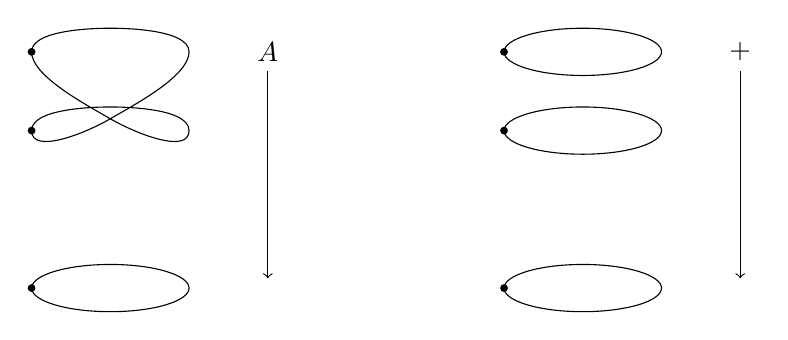
\begin{tikzpicture}
    \node (A) at (2,1) {$A$};
    \node (B) at (2,-2) {$\Sc$};
    \draw[->] (A) -- (B);
    \draw (0,-2) ellipse (1 and .3);
    \draw (-1,0)
    .. controls ++( 90:-.3) and ++(210: .4) .. (0,0.15)
    .. controls ++(210:-.4) and ++(270: .3) .. (1,1)
    .. controls ++(270:-.3) and ++(  0: .1) .. (0,1.3)
    .. controls ++(  0:-.1) and ++( 90: .3) .. (-1,1)
    .. controls ++( 90:-.3) and ++(150: .4) .. (0,0.15)
    .. controls ++(150:-.4) and ++(270: .3) .. (1,0)
    .. controls ++(270:-.3) and ++(  0: .1) .. (0,0.3)
    .. controls ++(  0:-.1) and ++( 90: .3) .. (-1,0);
    \node[fill,circle,inner sep=1pt] at (-1,-2) {};
    \node[fill,circle,inner sep=1pt] at (-1,0) {};
    \node[fill,circle,inner sep=1pt] at (-1,1) {};
%    \node (L) at (1,-3) {(left)};
    \begin{scope}[xshift=6cm]
    \node (At) at (2,1) {$\Sc+\Sc$};
    \node (Bt) at (2,-2) {$\Sc$};
    \draw[->] (At) -- (Bt);
    \draw (0,-2) ellipse (1 and .3);
    \draw (0,0) ellipse (1 and .3);
    \draw (0,1) ellipse (1 and .3);
    \node[fill,circle,inner sep=1pt] at (-1,-2) {};
    \node[fill,circle,inner sep=1pt] at (-1,0) {};
    \node[fill,circle,inner sep=1pt] at (-1,1) {};
%    \node (Lt) at (1,-3) {(right)};
    \end{scope}
  \end{tikzpicture}
  \end{sidecaption}
\end{figure}

\begin{remark}
  It \emph{is} possible to misunderstand what a ``connected \covering'' is:
the other interpretation ``all the preimages are connected''
would simply give us an equivalence (since connected sets are contractible),
and this is \emph{not} what is intended. (Equivalences are \coverings,
but not necessarily connected \coverings and connected \coverings are not neccesarily equivalences.)

Likewise for the other qualifications; for instance, in a ``finite covering'' $f:A\to B$,
the type $A$ is usually \emph{not} a finite set.

We trust the reader to keep our definitions in mind and not the other interpretations.
\end{remark}


\begin{remark}
  \Coverings are closely related to a concept from topology called ``covering spaces''
(or any variant of this concept, including Galois theory) and from algebra as locally constant sheaves (of sets).
Either way, the concept is useful because it singles out the (sub)symmetries.
\end{remark}

In this chapter, we focus on \coverings over the circle.

\begin{theorem}\label{thm:coveringsofS1perms}
  The evaluation function provides an equivalence
  \[
    \ev_\Set : (\Sc \to \Set) \to \sum_{X:\Set}(X=X)
    \quad\text{defined by $\ev_\Set(E) \defeq (E(\base),E(\Sloop))$.}
  \]
  Consequently, we have a string of equivalences
  \begin{align*}
    \SetBundle(\Sc)
    &\equiv (\Sc \to \Set)
      \equiv \sum_{X:\Set}(X=X) \\
    &\equiv \sum_{X:\Set}(X\equiv X)
    \equiv \sum_{X:\UU}\sum_{f:X\to X}
    \isset(X) \times \isEq(f).
  \end{align*}
\end{theorem}
\begin{proof}
  The first part is the universal property of the circle,
  \cref{lem:freeloopspace}, applied to $A\defeq\Set$.
  The equivalences then follow from \cref{lem:Prop-Set-pointed-families}\ref{lem:Set-families} and the univalence axiom,
  together with minor manipulations.
\end{proof}
In slogan form: A \covering over the circle is a set with a permutation of its elements.
The fiber over $\base:\Sc$ gives the set,
and transporting along $\Sloop$ gives the permutation.

A particularly important example is the following:
\begin{definition}\label{def:RtoS1}
  The \covering $R:\Sc\to\UU$ corresponds to the integers with the successor operation.
  We have $R(\base)\defeq\zet$ and $R(\Sloop)\defis \etop{\zs}$.
  (This is indeed a set bundle since $\Sc$ is connected,
  so that $R(x)$ is a set for all $x:\Sc$.
  Abusing notation we also write $R:\Sc\to\Set$.)
  Now define
  \[
    \tilde R\defeq\sum_{z:\Sc}R(z)
  \]
  and let the first projection denoted by
  \[
    \exp:\tilde R \to \Sc
  \]
  be the \emph{exponential \covering of the circle}.
\end{definition}

\begin{remark} \label{rem:expforreal}%
  \begin{marginfigure}
    \begin{tikzpicture}[scale=.15]
      \node (Sc) at (0,-5) {$\Sc$};
      \node[dot,label=left:$2$]  (B)    at (-10,18) {};
      \node[dot,label=left:$1$]  (one)  at (-10,14) {};
      \node[dot,label=left:$0$]  (zero) at (-10,10) {};
      \node[dot,label=left:$-1$] (mone) at (-10, 6) {};
      \node[dot,label=left:$-2$] (C)    at (-10, 2) {};
      \node[dot]                 (D)    at (-10,-5) {};
      \node[label=above:$\tilde R$]   (R)    at (10,20) {};
      \node[label=above left:$\zet$]  (Z)    at (-10,20) {};
      \node at (-10,20.8) {$\vdots$};
      \node at (-10,.2) {$\vdots$};
      \node[label=left:$\Sloop$] (Sloop) at (10,-5) {};

      \pgfmathsetmacro\cc{.55228475}% = 4/3*tan(pi/8)
      \pgfmathsetmacro\cy{2*\cc}%
      \pgfmathsetmacro\cx{10*\cc}%
      \pgfmathsetmacro\ay{.35165954}%

      \draw (10,0) \foreach \y in {0,4,...,16} {
        .. controls (10,\y + \cy + \ay) and (\cx,3 + \y - \ay)
        .. (0,3 + \y) .. controls (-\cx,3 + \y + \ay) and (-10,2 + \y + \cy - \ay)
        .. (-10,2 + \y) .. controls (-10,2 + \y - \cy + \ay) and (-\cx,1 + \y - \ay)
        .. (0,1 + \y) .. controls (\cx,1 + \y + \ay) and (10,4 + \y - \cy - \ay)
        .. (10,4 + \y) } ;
      \draw (10,-5) .. controls (10,-5 + \cy) and (\cx,-3)
      .. (0,-3) .. controls (-\cx,-3) and (-10,-5 + \cy)
      .. (-10,-5) .. controls (-10,-5 - \cy) and (-\cx,-7)
      .. (0,-7) .. controls (\cx,-7) and (10,-5 - \cy) .. (10,-5);
    \end{tikzpicture}
  \end{marginfigure}
  The reason for the name ``exponential'' comes from the following
  visualization.  If $x$ is a real number, then the complex
  exponentiation $\ee^{2\pi\ii x}=\cos(2\pi x)+\ii\sin(2\pi x)$ has
  absolute value $1$ and so defines a continuous function from the
  real numbers to the unit circle.  Choosing any point $z$ on the unit
  circle, we see that the preimage of $z$ under the exponential
  function is a shifted copy of the integers inside the reals.\footnote{%
    Again, we emphasize that we are here dealing with the
    \emph{homotopy types} of the reals $\RR$ and the unit circle,
    $\setof{(x,y):\RR^2}{x^2+y^2=1}$.}

  This connection between the integers and the unit circle is
  precisely captured in a form that we can take further by studying the
  \covering $\exp:\tilde R\to \Sc$.
\end{remark}

We already defined a \covering $f:A\to B$ to be universal if $A$ is connected
and all $a=_A a$ (for $a:A$) are connected.
If moreover $B$ is a pointed, connected groupoid we shall argue that
we actually can speak of \emph{the} universal \covering.

Recall \cref{cor:fib-vs-path} stating that all the fibers of a map $f:A\to B$
are sets if and only if each
\[
\ap{f}: (a=a')\to (f(a)=f(a'))
\]
is an injection.
Assume $f:A\to B$ is a universal \covering and $B$ is a groupoid.
We prove that $A$ is contractible.
Being contractible is a proposition, so we may assume
we have an element $a$ of $A$ since $A$ is connected.
By \cref{xca:connected-trivia} and \ref{xca:component-connected}
it suffices to prove that $a=a$ is contractible.
By \cref{xca:prop-set-trivia-2}, using that $a=a$ is connected,
it suffices to show that $a=a$ is a set.
Using that $\ap{f}$ is an injection, we can apply the remark after
\cref{lem:sum-of-fibers} and obtain that $a=a$ is a set since
$f(a)=f(a)$ is a set, since $B$ is a groupoid.
This completes the proof that $A$ is contractible.

Now assume $(B,b_0)$ is a pointed connected groupoid and $f:A\to B$
a universal \covering. Since $A$ and $\sum_{b:B}(b_0=_Bb)$ are both
contractible, and $B$ is connected, we have
$\Trunc{(A,f)=(\sum_{b:B}(b_0=_Bb),\fst)}$.
Hence if $(B,b_0)$ is a pointed connected groupoid, all
universal \coverings can be merely identified with a canonical one.
Moreover, the type of universal \coverings is equivalent to
$\bn 1 \to B$, and hence to $B$ itself,
so the type of \emph{pointed} universal \coverings is contractible.
This justifies the following definition.
\begin{definition}
  \label{def:universalcover}
  Let $(B,b_0)$ be a pointed connected groupoid.
  The \emph{universal \covering} of $B$
  is the \covering of $B$ given by the family of sets
  \[
    \uc{b_0}:B\to\Set,\quad \uc{b_0}(b)\defequi (b_0=_Bb),
  \]
  or alternatively as the first projection from
  $\uc{b_0}B\defequi\sum_{b:B}(b_0=_Bb)$ to $B$.

  This is canonically pointed at $(b_0,\refl{b_0}) : \sum_{b:B}(b_0=_Bb)$.
\end{definition}
Note that, for a general pointed connected type $(B,b_0)$, we have that
$(b_0=_B b)$ is a family of \emph{sets} exactly when $B$ is a groupoid.
The type family $(b_0=_B b)$ is also important if $B$ is not a groupoid,
but is then not a \emph{set} bundle.\footnote{%
  Of course, the type $\sum_{b:B}(b_0=b)$ is contractibe
  by \cref{lem:thepathspaceiscontractible}, for any type $B$.}

\begin{remark}
  What's so ``universal'' about this?
The universal \covering over the pointed connected groupoid $(B,b_0)$ coincides with the constant function $\cst{b_0}:\bn 1\to B$ (with value $b_0$), and seems like an unnecessary complicated representation were it not for the manifold practical value of the formulation that we've given.
In particular, we recognize the set of symmetries $b_0=_Bb_0$ as the preimage of $b_0$ under the first projection from $\uc{b_0}B$ to $B$; ultimately this will show that the study of symmetries coincides with the study of the universal \covering.

The first instance of this comes already in the next section, where we show in \cref{cor:S1groupoid} that the symmetries in the circle are given by the set of integers $\zet$ by showing that the universal \covering and the exponential \covering (\cref{def:RtoS1}) of the circle coincide.

That said, one way to see that the constant function $\cst{b_0}:\bn 1\to B$
\emph{does} deserve the label universal is the following.\marginnote{%
  Any $(a_0,p) : f^{-1}(b_0)$ gives rise to a commutative diagram:
  \[
    \begin{tikzcd}[column sep=small,ampersand replacement=\&]
      \bn 1\ar[rr,dashed,"\cst{a_0}"]\ar[dr,"\cst{b_0}"'] \& \& A \ar[dl,"f"] \\
      \& B \&
    \end{tikzcd}
  \]}
Given any function $f:A\to B$ and $(a_0,p): f^{-1}(b_0)$,
we get a function $\cst{a_0}:\bn 1\to A$, and $p:b_0=f(a_0)$ gives rise to
an element in $\cst{b_0}=_{\bn 1\to B}f \circ \cst{a_0}$.
In other words, any such $f$ is ``a factor of $\cst{b_0}$''.
Note, however, that this depends on $f^{-1}(b_0)$ being non-empty
(classically, this is often demanded of a covering, which distinguishes it from our \coverings),
and the factorization depends on the element $(a_0,p)$ used.

The situation is even simpler for pointed maps:
For any \emph{pointed} map $f : A \ptdto B$, with $(a_0,f_0):f^{-1}(b_0)$,
there is a \emph{unique} pointed map $g : \bn 1 \ptdto A$
(given by the base point of $A$), and this of course also gives
the unique way to write $f$ as a ``pointed factor of $\cst{b_0}$''.
\end{remark}

We'll continue the general study of set bundles in \cref{sec:gsets}
and indeed throughout the book.
For now, we'll focus our attention on the circle and set bundles over it.

\section{The symmetries in the circle}
\label{sec:symcirc}

With the set $\zet$ of integers \emph{defined} as in \cref{sec:integers},
we will now \emph{prove} that $\zet$ is equivalent to the type
$\base=_{\Sc}\base$, and that under this equivalence $0:\zet$ corresponds to
$\refl{\base}:\base=\base$, and $1$ to $\Sloop$, and $-1$ to $\Sloop^{-1}$.
More generally, the successor $\zs:\zet\to\zet$ corresponds to composition with $\Sloop$,
while the predecessor $\inv{\zs}$ corresponds to composition with $\Sloop^{-1}$.\marginnote{
  It follows directly that \emph{addition} of integers corresponds
  to \emph{composition} of loops.}

The first step is to prove that the exponential \covering \cref{def:RtoS1}
is equal to the universal \covering in \cref{def:universalcover},
\ie we prove that the family
\[
  R: \Sc\to\UU,\qquad R(\base)\defeq\zet,\, R(\Sloop)\defis \etop{\zs}
\]
is equal to the family
\[
\uc{\base}:\Sc\to\UU,\qquad \uc{\base}(z)\defeq (\base=z).
\]
What does it mean for the families $\uc{\base}$ and $R$ to be equal?
Type families are a special case of functions.
Function extensionality reduces the question to pointwise equality
of $\uc{\base}$ and $R$ as functions.
Using univalence, it suffices to give
an equivalence from $\uc{\base}(z)$ to $R(z)$ for every $z:\Sc$,
that is, recalling \cref{def:function-type-families},
a (fiberwise) equivalence $f: \uc{\base}\to R$. We will use
\cref{lem:weq-iso}, so will also define $g: R\to\uc{\base}$.

We first recall from \cref{sec:heavy-transport} how
transport behaves in families of function types.
Given a type $A$ and two type families $P,Q:A\to\UU$,
transport along $p:a=_Aa'$ of $h:P(a)\to Q(a)$ is
$Q(p)\,h\,P(p)^{-1}:P(a') \to Q(a')$.
In a picture,
\[
  \begin{tikzcd}[column sep=huge]
    a\ar[d,eqr,"p"] & P(a)\ar[r,"h"]\ar[d,eqr,"P(p)"] &
    Q(a)\ar[d,eqr,"Q(p)"] \\
    a' & P(a') & \,Q(a').
  \end{tikzcd}
\]
If $A$ is $\Sc$, then the induction principle for the circle says
that giving an $h(z):P(z)\to Q(z)$ for all $z:\Sc$ is the same as
specifying an $h(\base):P(\base)\to Q(\base)$ and,
using \cref{def:pathover-trp} and the discussion above, an identity
$h(\Sloop):Q(\Sloop)\,h(\base)\,P(\Sloop)^{-1}=_{P(\base)\to Q(\base)}h(\base)$,
\ie   a witness that the composites in
\[
  \begin{tikzcd}[column sep=huge]
    P(\base)\ar[r,"h(\base)"]\ar[d,eqr,"P(\Sloop)"]
    & Q(\base)\ar[d,eqr,"Q(\Sloop)"] \\
    P(\base)\ar[r,"h(\base)"] & Q(\base)
  \end{tikzcd}
\]
are equal. If $P,Q$ are families of sets,
then the type of $h(\Sloop)$ is a proposition.

We now define $f: \uc{\base}\to R$ and $g: R\to\uc{\base}$ that will turn out to
give inverse equivalences between $\uc{\base}(z)$ and $R(z)$, for each $z:\Sc$.

\begin{marginfigure}
  \begin{tikzpicture}[scale=.15]
    \node (Sc) at (0,-5) {$\Sc$};
    \node[dot,label=above:$\vdots$] (B)    at (-10,18) {};
    \node[dot]                      (one)  at (-10,14) {};
    \node[dot]                      (zero) at (-10,10) {};
    \node[dot]                      (mone) at (-10, 6) {};
    \node[dot]                      (C)    at (-10, 2) {};
    \node[dot]                      (D)    at (-10,-5) {};
    \node[label=above:$\RR$]        (R)    at (10,20) {};
    \node[label=above left:$\zet$]  (Z)    at (-10,20) {};
    \node at (-10,.2) {$\vdots$};
    \node[label=left:$\Sloop$] (Sloop) at (10,-5) {};

    \pgfmathsetmacro\cc{.55228475}% = 4/3*tan(pi/8)
    \pgfmathsetmacro\cy{2*\cc}%
    \pgfmathsetmacro\cx{10*\cc}%
    \pgfmathsetmacro\ay{.35165954}%

    \draw (10,0) \foreach \y in {0,4,...,16} {
      .. controls (10,\y + \cy + \ay) and (\cx,3 + \y - \ay)
      .. (0,3 + \y) .. controls (-\cx,3 + \y + \ay) and (-10,2 + \y + \cy - \ay)
      .. (-10,2 + \y) .. controls (-10,2 + \y - \cy + \ay) and (-\cx,1 + \y - \ay)
      .. (0,1 + \y) .. controls (\cx,1 + \y + \ay) and (10,4 + \y - \cy - \ay)
      .. (10,4 + \y) } ;
    \draw (10,-5) .. controls (10,-5 + \cy) and (\cx,-3)
    .. (0,-3) .. controls (-\cx,-3) and (-10,-5 + \cy)
    .. (-10,-5) .. controls (-10,-5 - \cy) and (-\cx,-7)
    .. (0,-7) .. controls (\cx,-7) and (10,-5 - \cy) .. (10,-5);

    \draw[->, bend left, shorten <=2pt, shorten >=2pt] (zero) to
    node[left] {\scriptsize$\trp[R]{\Sloop}$} (one);%
    \draw[->, bend right, shorten <=2pt, shorten >=2pt] (zero) to
    node[left] {\scriptsize$\trp[R]{\inv\Sloop}$} (mone);%
    \draw[->, bend right, shorten <=2pt, shorten >=2pt, line
    width=2pt, white] (zero) to (B);%
    \draw[->, bend right, shorten <=2pt, shorten >=2pt] (zero) to
    node[right,rounded corners,fill=white,outer sep=5pt]
    {\scriptsize$\trp[R]{\Sloop^2}$} (B);%
    \draw[->, bend left, shorten <=2pt, shorten >=2pt, white, line
    width=2pt] (zero) to (C);%
    \draw[->, bend left, shorten <=2pt, shorten >=2pt] (zero) to
    node[right,rounded corners,fill=white,outer sep=5pt]
    {\scriptsize$\trp[R]{\Sloop^{-2}}$} (C);
  \end{tikzpicture}
  \caption{Transport in the family $R$}\label{fig:transportalongloop}
\end{marginfigure}
\begin{definition}
  \label{def:fPtoR}
  The function $f:\prod_{z:\Sc}(\uc{\base}(z)\to R(z))$ is defined by transport: $f(z)(p)\defequi\trp[R]{p}(0)$.
\end{definition}
In Figure~\ref{fig:transportalongloop}, the transport in the definition
above has been visualised for $p={\Sloop^n}$, $n=-2,-1,0,1,2$.

\begin{lemma}\label{lem:windingnumber}
For $f$ as in \cref{def:fPtoR} we have $f(\base)(\Sloop^n)=n$ for all $n:\zet$.
\end{lemma}
\begin{proof}
First consider positive $n:\NN$ and apply induction. In the base case $n=0$ we have
$f(\base)(\Sloop^0)\jdeq f(\refl\base)\jdeq\trp[R]{\refl\base}(0) \jdeq 0$.
For $n=\zs(m)$ with $m:\NN$ we have
\begin{align*}
  f(\base)(\Sloop^{\zs(m)})
  &\jdeq\trp[R]{\Sloop^{\zs(m)}}(0)\\
  &=\trp[R]{\Sloop \Sloop^{m}}(0)\\
  &=\trp[R]{\Sloop}(\trp[R]{\Sloop^m}(0))\\
  &\jdeq \trp[R]{\Sloop}(f(\base)(\Sloop^{m}))\\
  &= \zs(f(\base)(\Sloop^{m})).
\end{align*}
The last step follows from $\etop{\zs}=R(\Sloop)$
and $\zs=\trp[\id_\UU]{\etop{\zs}}$, see \cref{def:univalence},
and hence $\zs=\trp[\id_\UU]{R(\Sloop)}=\trp[\id_\UU R]{\Sloop}=\trp[R]{\Sloop}$.
This completes the induction step for positive $n$.
For negative $n$ the proof is similar.
\end{proof}

In the definition of the second map,
take into account that $R(\base)\jdeq \zet$ and $\uc{\base}(\base) \jdeq (\base=\base)$.

\begin{definition}\label{def:gRtoP}
The function $g:\prod_{z:\Sc}(R(z)\to \uc{\base}(z))$ is
defined by circle induction:
\[
g(\base)\defeq \left(n \mapsto {\Sloop^n} \right) :\zet\to(\base=\base)
\]
and
\[
g(\Sloop): \uc{\base}(\Sloop)\, g(\base)\,R(\Sloop)^{-1}=_{\zet\to (\base=\base)} g(\base).
\]
\marginnote{%
  In a picture, $g(\Sloop)$ should prove that it does not matter what
  path you take around the square
  \[
    \begin{tikzcd}[row sep=large,column sep=huge,ampersand replacement=\&]
      \zet\ar[r,"\Sloop^-"]\ar[d,eqr,"\zs"] \&
      (\base=\base)\ar[d,eqr,"\Sloop\cdot\blank"] \\
      \zet\ar[r,"\Sloop^-"] \& (\base=\base).
    \end{tikzcd}
  \]
}%
So far we have only given the type of $g(\Sloop)$. By definition,
$R(\Sloop)$ is $\zs$ and $\uc{\base}(\Sloop)$ is composition with
$\Sloop$.
The element $g(\Sloop)$ follows by a simple calculation: the
proposition ${\Sloop\,\Sloop^{n-1}} = {\Sloop^n}$ holds for all
$n:\zet$.
\end{definition}


\begin{theorem}
  \label{lem:univisexp}
For every $z:\Sc$, the functions $f(z)$ defined in \cref{def:fPtoR}
and $g(z)$ in \cref{def:gRtoP} are inverse equivalences between
$\uc{\base}(z)$ and $R(z)$.
\end{theorem}
\begin{proof}
We apply \cref{lem:weq-iso} and verify the two conditions.
  First, we need to give elements $H(z,p):g(z)(f(z)(p))=p$
for all $z:\Sc$ and $p:\uc{\base}(z)\jdeq(\base=z)$.
By induction on $p:\base=z$ it suffices to set
$H(\base,\refl\base)\defeq\refl{\refl{\base}}$ since
$g(\base)(f(\base)(\refl{\base}))\jdeq g(\base)(0)\jdeq\refl{\base}$.

Secondly, we need to give elements $G(z)(n):f(z)(g(z)(n))=n$
for all $z:\Sc$ and $n: R(z)$.
By circle induction it suffices to define $G(\base)$ and $G(\Sloop)$,
but since $\zet$ is a set the information for $G(\Sloop)$ is redundant.
Hence, we need to show that for all $n:\zet$ that
$f(\base)(g(\base)(n))\jdeq  f(\base)(\Sloop^n)$ is equal to $n$.
This follows from \cref{lem:windingnumber}.
\end{proof}


\begin{corollary}\label{cor:S1groupoid}
The circle $\Sc$ is a groupoid, and the function
\[
{\Sloop}^{\blank} : \zet\to(\base=_{\Sc}\base)
\]
sending $n$ to $\Sloop^n$ is an equivalence.
\end{corollary}
\begin{proof}
For any $z:\Sc$, the type $\uc{\base}(z)\jdeq (\base=_{\Sc}z)$ is a set
since $R(z)$ is a set and $\uc{\base}(z) \equiv R(z)$.
Since the circle is connected and being a set is a proposition, it follows
that $y=_{\Sc}z$ is a set, for any $y,z:\Sc$. Hence $\Sc$ is a groupoid.
By \cref{def:gRtoP}, ${\Sloop}^{-}\jdeq g(\base)$ is an equivalence.
\end{proof}
\begin{definition}\label{def:windingnumber}
  The inverse function of ${\Sloop}^{\blank}$
  is called the \emph{winding number} function
  $\wdg : (\base =_\Sc\base) \to \zet$.
\end{definition}
The following lemma is a simple example of a technique later called \emph{delooping}.
\begin{lemma}\label{lem:S1-delooping}
Let $A$ be a connected type and $a:A$.
Assume we have an equivalence $e:(\base=_{\Sc}\base) \to (a=a)$
of symmetries such that $e(\refl{\base})=\refl{a}$
and $e(p\cdot q)=e(p)\cdot e(q)$, for all $p,q:(\base=_{\Sc}\base)$.
Then $\check e : \Sc\to A$ defined by circle recursion by setting
$\check e(\base)\defeq a$ and $\check e(\Sloop)\defis e(\Sloop)$
is an equivalence.
\end{lemma}
\begin{proof}
We have $\ap{\check e} = e$ since they produce equal values when applied
to $\Sloop^n$, for all $n:\zet$. Now use that $A$ and $\Sc$ are connected and
apply \cref{cor:fib-vs-path}\ref{conn-fib-vs-path}.
\end{proof}

\begin{xca}\label{xca:general-winding}
  Using circle induction, define for any point $x:\Sc$ of the circle
  an equivalence, $\wdg_x : (x =_\Sc x) \we \zet$,
  generalizing~\cref{def:windingnumber}.
  (You'll need commutativity of addition in $\zet$.)
  Conclude from \cref{lem:S1-delooping} that we have equivalences
  $f_x : \Sc \we \Sc$ with $f_x(\base) \jdeq x$, for each $x:\Sc$.\footnote{%
    If we think of the circle as represented by the unit length complex numbers,
    then $f_x(y)$ corresponds to the usual product $xy$.}
\end{xca}

\section{A reinterpretation of the circle}\label{sec:S1isC}

In this section we return to the equivalences in \cref{thm:coveringsofS1perms}.
We'll use these to get a different perspective on the circle,
which highlights it as a type classifying very simple symmetries,
namely sets with permutations.
We have already seen one example in \cref{def:RtoS1},
namely the set $\zet$ of integers together with the successor $\zs: \zet\equiv\zet$,
corresponding to the universal \covering $\uc\base:\Sc \to \Set$,
which as a map is the constant function $\cst\base : \bn 1 \to \Sc$.

The importance of the latter example will become apparent when we eventually
explain that \emph{the circle is equivalent to the connected component of
  $(\zet,\zs)$ in the type $\sum_{X:\UU}(X\to X)$}.\footnote{%
  The elements of this connected component can be thought of as
  \emph{infinite cycles}:
  sets $X$ with a successor function $t:X \to X$
  such that $(X,t)$ can be merely identified with $(\zet,\zs)$.
  That is, $(X,t)$ looks exactly like $(\zet,\zs)$,
  but we don't know which element of $X$ is ``zero'':\\[1ex]
  \begin{tikzpicture}[node distance=10pt]
    \begin{scope}[every node/.style={dot}]
      \node (x1) {};
      \foreach \p/\n/\deg in {1/2/27, 2/3/54, 3/4/81, 4/5/108, 5/6/135,%
        6/7/162, 7/8/135, 8/9/108, 9/10/81, 10/11/54, 11/12/27} {
        \node (x\n) [at=(x\p.\deg), anchor=\deg+180, shift=(\deg:10pt)] {};
      }
    \end{scope}
    \node (x0) [left=of x1] {$\ldots$};
    \node (x13) [right=of x12] {$\ldots$};
    \begin{scope}[->,shorten <=1pt,shorten >=1pt]
      \foreach \p/\n in {0/1, 1/2, 2/3, 3/4, 4/5, 5/6,
        6/7, 7/8, 8/9, 9/10, 10/11, 11/12, 12/13} {
        \draw (x\p)--(x\n);
      }
    \end{scope}
  \end{tikzpicture}}

The key of course is that the equivalences in \cref{thm:coveringsofS1perms}
restrict to equivalences between their connected components,
so to understand the components of $\SetBundle(\Sc)$
it suffices to understand the components of $\sum_{X:\UU}(X \to X)$ at pairs $(X,t)$,
where $X$ is a set with a permutation $t$.

We are particularly interested in understanding the symmetries in these components,
so before we prove that the circle is equivalent to the component containing $(\zet,\zs$),
let us investigate the equalities in the type $\sum_{X:\UU}(X \to X)$ a bit further.

Define the type family $D$ by $D(X) \defeq (X\to X)$ for all $X:\UU$.
Recall from \cref{lem:isEq-pair=} that, given $X,Y:\UU$ and $t:X\to X$ and $u:Y\to Y$,
the identity type $(X,t)=(Y,u)$
is equivalent to the type of pairs consisting of a $p:X=Y$ and
an element of $\pathover{t}{D}{p}{u}$. The latter type is
equivalent to $\trp[D]{p}(t) = u$ by \cref{def:pathover-trp}.
The transport is by conjugation,
\cref{lem:trp-in-function-type}, so that the latter
type is equivalent to $\ptoe p\circ t\circ \ptoe p^{-1} = u$.
If $p\jdeq\etop e$ for an equivalence $e:X\equiv Y$,
this is equivalent to $e\circ t = u\circ e$, or $e t = u e$ for short.
In total, the identity type $(X,t)=(Y,u)$ is equivalent to
\[
  \sum_{e: X\equiv Y} et =_{X\to Y} ue.
\]
This is a set whenever $X$ and $Y$ are; see \cref{fig:Zs=Xt} for an illustration.
\begin{marginfigure}
  \begin{tikzpicture}[node distance=10pt]
    \begin{scope}[every node/.style={dot}]
      \node (x1) {};
      \foreach \p/\n/\deg in {1/2/72, 2/3/54, 3/4/81, 4/5/108, 5/6/135,%
        6/7/162, 7/8/135, 8/9/108, 9/10/81, 10/11/54, 11/12/72} {
        \node (x\n) [at=(x\p.\deg), anchor=\deg+180, shift=(\deg:10pt)] {};
      }
      \node (y1) [at=(x1.east), anchor=180, shift=(192:50pt)] {};
      \foreach \p/\n in {1/2, 2/3, 3/4, 4/5, 5/6,%
        6/7, 7/8, 8/9, 9/10, 10/11, 11/12} {
        \node (y\n) [at=(y\p.north), anchor=south, shift=(90:10pt)] {};
      }
    \end{scope}
    \node (x0) [below=of x1] {$\vdots$};
    \node (y0) [below=of y1] {$\vdots$};
    \node (x13) [above=of x12] {$\vdots$};
    \node (y13) [above=of y12] {$\vdots$};
    \node (Xf)  [above=26pt of x12] {$(X,t)$};
    \node (Zs)  [left=2pt of y13] {$(\zet,\zs)$};
    \node (zero)  [left=2pt of y6] {$0$};
    \begin{scope}[->,shorten <=1pt,shorten >=1pt]
      \foreach \p/\n in {0/1, 1/2, 2/3, 3/4, 4/5, 5/6,
        6/7, 7/8, 8/9, 9/10, 10/11, 11/12, 12/13} {
        \draw (x\p)--(x\n);
        \draw (y\p)--(y\n);
      }
    \end{scope}
    \begin{scope}[casblue,<-,shorten <=1pt,shorten >=1pt]
      \foreach \n in {1,2,...,12} {
        \draw (x\n)--(y\n);
      }
    \end{scope}
  \end{tikzpicture}
  \caption{An identification of two infinite cycles.
    The equivalence $e : \zet \equiv X$ is marked in blue.}\label{fig:Zs=Xt}
\end{marginfigure}
In particular, the identity type $(\zet,\zs)=(X,t)$
is equivalent to the set $\sum_{e:\zet\equiv X}e\zs=te$, for any set $X$ with a permutation $t$.
Tautologically, then, any power $\zs^n$ of $\zs$ itself gives a symmetry
$(\zs^n,!) : (\zet,\zs)=(\zet,\zs)$.

The following property jumps out at us when we contemplate~\cref{fig:Zs=Xt}.
\begin{lemma}
  \label{lem:IdCisZet}
  An element $(e,!) : (\zet,\zs)=(X,t)$,
  with $(X,t)$ in the component of $(\zet,\zs)$,
  is uniquely determined by the element $e(0):X$.
  In other words, the function
  \[
    \ev_0:\bigl((\zet,\zs)=(X,t)\bigr)\to X
    \text{~~defined by~~} \ev_0(e,!) \defeq e(0)
  \]
  is an equivalence.
\end{lemma}
\begin{proof}
  We'll prove that every fiber of $\ev_0$ is contractible.
  Given $x_0:X$ we must determine a unique equivalence $e:\zet\to X$
  such that $es=te$ and $e(0)=x_0$.
  Induction on $n:\zet$ (positive and negative $n$ separately)
  shows that for such an $e$, we have $e(n) = t^n(x_0)$ for all $n:\zet$.
  It remains to prove that this is an equivalence.
  More precisely, it suffices to prove the proposition:
  \begin{displaymath}
    \prod_{x_0:X} \isEq(n\mapsto t^n(x_0))
  \end{displaymath}
  Since we are proving a proposition,
  and we are assuming $(X,t)$ is in the component of $(\zet,\zs)$,
  it suffices to prove it for $(X,t) \jdeq (\zet,\zs)$.
  However, for any $x_0:\zet$,
  the map $n \mapsto \zs^n(x_0) = n + x_0$ is an equivalence,
  with inverse $n \mapsto n - x_0$.
\end{proof}
In particular, the identity type $(\zet,\zs)=(\zet,\zs)$ is equivalent to $\zet$.

\begin{definition}\label{def:S1toC}
  Let $\InfCyc$ be the component of $\sum_{X:\UU}(X\to X)$ containing $(\zet,\zs)$.
  Elements of $\InfCyc$ are called \emph{infinite cycles}.\footnote{%
    See also~\cref{def:Cyc} below for general cycles.}

  Define by circle induction
  \[
    c:\Sc\to\InfCyc \text{~~setting~~}
    c(\base)\defequi (\zet,\zs)
  \]
  and $c(\Sloop): c(\base)= c(\base)$ given by the \emph{predecessor} equivalence
  $\zs^{-1}:\zet\to\zet$
  and the trivial proof of the proposition $\zs^{-1}\zs=\zs\zs^{-1}$.
\end{definition}
\begin{marginfigure}
  \noindent\begin{tikzpicture}[scale=.15]
    \node (Sc) at (0,-5) {$\Sc$};
    \node[dot]                 (D)    at (-10,-5) {};
    \node[label=above left:$\uc{\color{casred}\base}({\color{casblue}\base})$] (Z) at (-10,20) {};
    \node at (-10,24.8) {$\vdots$};
    \node at (-10,.2) {$\vdots$};
    \node[label=left:$\Sloop$] (Sloop) at (10,-5) {};

    \pgfmathsetmacro\cc{.55228475}% = 4/3*tan(pi/8)
    \pgfmathsetmacro\cy{2*\cc}%
    \pgfmathsetmacro\cx{10*\cc}%
    \pgfmathsetmacro\ay{.35165954}%

    \draw[dashed] (10,0)
    .. controls (10,\cy + \ay) and (\cx,3 - \ay)
    .. (0,3) .. controls (-\cx,3 + \ay) and (-10,2 + \cy - \ay)
    .. (-10,2);
    \foreach \y/\col in {0/dashed,4/casred,8/black,12/casblue,16/dashed} {
      \draw[\col] (-10,2 + \y)
      .. controls (-10,2 + \y - \cy + \ay) and (-\cx,1 + \y - \ay)
      .. (0,1 + \y) .. controls (\cx,1 + \y + \ay) and (10,4 + \y - \cy - \ay)
      .. (10,4 + \y) .. controls (10,4 + \y + \cy + \ay) and (\cx,7 + \y - \ay)
      .. (0,7 + \y) .. controls (-\cx,7 + \y + \ay) and (-10,6 + \y + \cy - \ay)
      .. (-10,6 + \y);
    }
    \draw[dashed] (-10,22)
    .. controls (-10,22 - \cy + \ay) and (-\cx,21 - \ay)
    .. (0,21) .. controls (\cx,21 + \ay) and (10,24 - \cy - \ay)
    .. (10,24);
    \foreach \y in {2,6,...,22} {
      \node[dot] (B\y) at (-10,\y) {};
    }
    \draw (10,-5) .. controls (10,-5 + \cy) and (\cx,-3)
    .. (0,-3) .. controls (-\cx,-3) and (-10,-5 + \cy)
    .. (-10,-5) .. controls (-10,-5 - \cy) and (-\cx,-7)
    .. (0,-7) .. controls (\cx,-7) and (10,-5 - \cy) .. (10,-5);
  \end{tikzpicture}
  \caption{For the fiber of the universal \covering,
    $\uc{\color{casred}\base}({\color{casblue}\base}) \jdeq
    ({\color{casred}\base} = {\color{casblue}\base})$,
    we \emph{increase} the winding number when we transport
    the endpoint (in blue) along $\Sloop$, and
    we \emph{decrease} it when we transport the starting point
    (in red) in the same way.}\label{fig:plus-minus-one}
\end{marginfigure}

Note that, as usual, we leave out the propositional components of $\InfCyc$ (and other subtypes) from the notation.

Since it's such a crucial result, we are going to give two proofs that $c$ from \cref{def:S1toC} is an equivalence.
Each proof illuminates a different aspect and gives methods that will be used later.

For the first, we return to the equivalences of \cref{thm:coveringsofS1perms}.
As we said above, these restrict to equivalences between the different components.
In particular, $\ev_\UU : (\Sc \to \UU) \to
\sum_{X:\UU}X=X$ maps the type family $\uc{\base}$ to the pair
$(\base = \base, q\mapsto {{\Sloop}\cdot q})$,
which can be identified with $(Z,s)$ through~\cref{cor:S1groupoid}.
Hence, $\ev_\UU$ restricts to an equivalence between the
connected component of $\uc\base$ in $\Sc \to \UU$ and the connected component
of $(Z,s)$ in $\sum_{X:\UU}X=X$.
We claim that we get a commuting diagram
\begin{equation}\label{eq:setbundle-Sc-univ-comp}
  \begin{tikzcd}
    & \Sc\ar[dl,"\cst{\blank}"']\ar[d,"\uc{\blank}"]\ar[dr,"c"] & \\
    \conncomp{\SetBundle(\Sc)}{\cst\base} \ar[r,"\sim"]
    & \conncomp{(\Sc\to\UU)}{\uc\base} \ar[r,"\sim","\ev_\UU"']
    & \InfCyc,
  \end{tikzcd}
\end{equation}
where the left-most diagonal arrow maps $z:\Sc$ to the constant map $\cst z:\bn 1\to\Sc$.
The left-hand triangle commutes, because the fiber $\sum_{\_:\bn 1}(x=z)$
of $\cst z$ at $x:\Sc$ is equivalent to $\uc{z}(x) \jdeq (z=x)$.
We prove that the right-hand triangle commutes by circle induction.
That is, we show $\prod_{z:\Sc}c(z) = \ev_\UU(\uc{z})$.
The case $z\jdeq\base$ is exactly the equivalence
$g(\base)\jdeq{\Sloop^-} : \zet \to \uc{\base}(\base)$ of \cref{lem:univisexp}
together with the fact that $\trp[\uc\base]{\Sloop}$ corresponds to $\zs$.
To finish, we observe that it doesn't matter which way you take in the diagram
\[
  \begin{tikzcd}[row sep=large,column sep=huge]
    \zet\ar[r,"\Sloop^-"]\ar[d,"\inv{\zs}"] &
    (\base=\base)\ar[d,"\blank\cdot\Sloop^{-1}"] \\
    \zet\ar[r,"\Sloop^-"] & (\base=\base).
  \end{tikzcd}
\]
Note that to transport in the family $\uc{-}(\base) \jdeq (\blank = \base)$,
we use \cref{xca:trp-in-a/x=b/x}\ref{trp-in-x=a},
and \emph{that} is why we picked the predecessor equivalence in~\cref{def:S1toC}.
This is also illustrated in \cref{fig:plus-minus-one}.\footnote{%
  Another option would have been to choose the opposite equivalence $\zet\equiv\uc\base(\base)$, sending $n$ to $\Sloop^{-n}$, in the base case.
  The point is: You can move the minus sign around, but it has to pop up somewhere.}

With~\eqref{eq:setbundle-Sc-univ-comp} in hand, we see that $c$ is an equivalence
if and only if either of the two other downward maps are.\footnote{%
  At this point we could conclude with an appeal to the type theoretic Yoneda lemma,
  which states that the map $X \to (X \to \UU)$,
  sending $x$ to the family $y \mapsto x=y$,
  is an injection for any type $X$.
  Exercise: Prove this!}
It is very direct to show that the map on the left is an equivalence.
Indeed, the identity type $(\bn 1,\cst x)=(\bn 1,\cst y)$
is equivalent to pairs of an equivalence $e : \bn 1 \to \bn 1$ and a commuting triangle
\[
  \begin{tikzcd}
    \bn 1 \ar[rr,"e"]\ar[dr,"\cst x"'] & & \bn 1\ar[dl,"\cst y"] \\
    & \Sc. &
  \end{tikzcd}
\]
But since $\bn 1$ is contractible, this just amounts to the equality $x=y$.
Hence the map is an embedding, and we conclude by \cref{cor:fib-vs-path}\ref{conn-fib-vs-path}.

We now give the second, more direct, proof that $c$ is an equivalence.
For this we use the following lemma, which is of independent interest.
\begin{lemma}\label{lem:conn-eq-f-ap-f-x}
Let $X$ and $Y$ be connected types, $x$ an element of $X$,
and $f$ a function from $X$ to $Y$. Then $f$ is an equivalence
if and only if $\ap{f}: (x=x) \to (f(x)=f(x))$ is an equivalence.
\end{lemma}
\begin{proof}
Using \cref{cor:fib-vs-path}\ref{conn-fib-vs-path} it suffices to show that
each map induced by $f$ on identity types is an equivalence if and only if the specific map
$\ap f : (x=x) \to (f(x) = f(x))$ is an equivalence.  Being an equivalence is a proposition,
so the result follows in two easy steps from $X$ being connected,
using \cref{xca:component-connected}.
\end{proof}

\begin{theorem}\label{thm:S1bysymmetries}
  The function $c:\Sc\to\InfCyc$ from \cref{def:S1toC} is an equivalence.
\end{theorem}
\begin{proof}
  In view of \cref{lem:conn-eq-f-ap-f-x} we only need to show that
$\ap{c}:(\base=_{\Sc}\base)\to((\zet,\zs)=(\zet,\zs))$ is an equivalence.
Note that both the domain and the co-domain of $\ap{c}$ are equivalent to $\zet$.
Consider the following diagram in which we compose $c$ with the equivalences
from \cref{cor:S1groupoid} and \cref{lem:IdCisZet}:
\[
  \begin{tikzcd}[column sep=large]
    \zet\ar[r,"\Sloop^-"] &
    (\base=\base)\ar[r,"\ap{c}"] &
    \bigl((\zet,\zs)=(\zet,\zs)\bigr)\ar[r,"\ev_0\vphantom{\ap{c}}"] &
    \zet
  \end{tikzcd}
\]
For $c$ to be an equivalence, it suffices to show that the composition
is an equivalence from $\zet$ to itself.
By definition, $\ap{c}(\Sloop)$ is the identification
corresponding to $\inv\zs$, sending $0$ to $-1$,
and by induction on $n:\zet$ it follows that
$\ev_0(\ap{c}(\Sloop^n)) = \zs^{-n}(0) = -n$.
And the map $n \mapsto -n$ is indeed an equivalence.
\end{proof}

\section{Connected \coverings over the circle}
\label{sec:covS1}

Let $A$ be a type and $f:A\to \Sc$ a function.
By \cref{cor:fib-vs-path}\ref{set-fib-vs-path}, $f$ is a \covering
over $\Sc$ if and only if each map induced by $f$ on identity types is injective.
Assume that $f:A\to \Sc$ is a \covering with $A$ connected.
Let $(a_0,p)$ be an element of $f^{-1}(\base)$.
By \cref{xca:component-connected}
the condition that \emph{each} $\ap{f}$ is injective
can be relaxed to $\ap{f}: (a_0=a_0)\to(f(a_0)=f(a_0))$ being injective.
Now look at the following subset:
\begin{equation}\label{eq:subgroup-covering-1}
  \setof{q: \base =_\Sc \base}{{\ap{f}}^{-1}(pqp^{-1})}.
\end{equation}
Clearly, a classification of connected \coverings over the circle
also classifies certain subsets of symmetries of $\base$,
or equivalently, using~\cref{cor:S1groupoid}, certain subsets of $\zet$.
Such subsets of $(\base=_\Sc\base)$ are closed under concatenation and inverses,
since $\ap{f}$ is compatible with these operations,
see \cref{lem:apcomp}.
Using language yet to be introduced, we actually ``classify the subgroups of the integers''.

Recall that \coverings over the circle are equivalent to sets with permutations.
Which sets with permutations $(X,t)$ correspond to connected \coverings?
It is not so surprising that the answer has to do with whether
any two points $x,x':X$ can be connected by applying $t$ some number of times.
\begin{definition}\label{def:Cyc}
  Let $\Cyc$ be the subtype of $\sum_{X:\UU}(X\to X)$ of those
  pairs $(X,t)$ where $X$ is a \emph{\nonempty} set with an \emph{equivalence} $t$
  such that for any $x,x':X$
  there exists some $n:\zet$ with $x' = t^n(x)$.\marginnote{%
    Recall that the iteration $t^n$ makes sense for all integers $n$
    since $t$ is an equivalence.}
  Elements of $\Cyc$ are called \emph{cycles}.\footnote{%
    Our cycles are a special case of what is elsewhere called
    \emph{cyclically ordered sets},
    and they are closely related to the \emph{cyclic sets} of
    \citeauthor{Connes1983}\footnotemark{}.}\footcitetext{Connes1983}
\end{definition}
\begin{theorem}\label{thm:cycset-connS1cover}
  Under the equivalence of \cref{thm:coveringsofS1perms},
  connected \coverings of the circle correspond to cycles.
\end{theorem}
\begin{proof}
  Consider a set $X$ with permutation $t$.
  The corresponding family of sets is $E\defeq\ve_\UU(X,\etop{t}) : \Sc\to\UU$,
  so the corresponding set bundle over the circle
  is the first projection, $\fst : A \to \Sc$,
  where we put $A\defeq\sum_{z:\Sc}E(z)$.
  We need to show that $A$ is connected if and only if $X$ is \nonempty
  and any two elements of $X$ can be connected by $t$.

  We show something a little more general, namely we give a bijection
  $g : \setTrunc A \to X/\sim$, from the set of components of $A$
  to the quotient set of $X$ by the equivalence relation $\sim$
  defined by $(x\sim x') \defeq \exists_{n:\zet}(x'=t^n(x))$.\footnote{%
    Exercise: Check that this defines an equivalence relation,
    and that the bijection $g$ proves the theorem.}

  We define $g$ using the universal property of set truncation (\cref{def:set-truncation}), pair induction, and circle induction.
  To define $g_0 : \prod_{z:\Sc}(E(z) \to X/\sim)$, we need
  $g_0(\base)\defeq[\blank] : X \to X/\sim$ and
  $g_0(\Sloop) : \pathover{g_0(\base)}{E(\blank) \to X/\sim}{\Sloop}{g_0(\base)}$,
  equivalent to $g_0(\base) =_{X \to X/\sim} g_0(\base)t$.
  The latter we get by function extensionality and \cref{thm:quotient-property},
  since $x \sim t(x)$ for any $x:X$.

  The inverse of $g$, $h:(X/\sim) \to \setTrunc A$,
  is defined as the extension of $h_0 : X \to \setTrunc A$
  with $h_0(x) \defeq \settrunc{(\base,x)}$.
  We just need to check that $h_0(x) = h_0(x')$, or equivalently,
  $\Trunc{(\base,x)=_A(\base,x')}$, whenever $x\sim x'$.
  Since this is a proposition, if $x'=t^n(x)$ with $n:\zet$,
  we may use induction on $n$ (positive and negative)
  together with the paths,
  $\pathpair{\Sloop}{\refl{f(x)}} : (\base,x)=(\base,t(x))$,
  to conclude.

  It's easy to check that $g$ and $h$ are mutually inverse.
\end{proof}
In \cref{fig:two-comp-S1-cover} we see the \covering corresponding
to the set $\set{1,2,3,4,5}$ with the permutation $1\mapsto 2\mapsto 3\mapsto 1,4\mapsto 5\mapsto 4$. There are two components, showing that the permutation splits into two cycles.
\begin{marginfigure}
  \begin{tikzpicture}[scale=.15]
    \node (Sc) at (0,-5) {$\Sc$};
    \node[dot,label=left:$5$] (four)  at (-10,22) {};
    \node[dot,label=left:$4$] (three) at (-10,18) {};
    \node[dot,label=left:$3$] (two)   at (-10,10) {};
    \node[dot,label=left:$2$] (one)   at (-10, 6) {};
    \node[dot,label=left:$1$] (zero)  at (-10, 2) {};
    \node[dot]                (D)     at (-10,-5) {};
    \node[label=left:$\Sloop$] (Sloop) at (10,-5) {};

    \pgfmathsetmacro\cc{.55228475}% = 4/3*tan(pi/8)
    \pgfmathsetmacro\cy{2*\cc}%
    \pgfmathsetmacro\cx{10*\cc}%
    \pgfmathsetmacro\intx{3.5}%
    \pgfmathsetmacro\inty{1.5}%
    \pgfmathsetmacro\ay{.35165954}%

    \draw (-10,18) .. controls (-10,18 - \cy + \ay) and (-\cx,17 - \ay)
    .. (0,17) .. controls (\cx,17 + \ay) and (10,20 - \cy - \ay) .. (10,20)
    .. controls (10,20 + \cy + \ay) and (\cx,23 - \ay)
    .. (0,23) .. controls (-\cx,23 + \ay) and (-10,22 + \cy - \ay)
    .. (-10,22) .. controls (-10,22 - \cy + \ay) and (-\cx,21 - \ay)
    .. (0,21) .. controls (\cx,21 + \ay) and (10,24 - \cy - \ay)
    .. (10,24)
    .. controls (10,24 + \cc) and (\intx + \cx, 24 + \inty + \ay)
    .. (\intx,24 + \inty) .. controls (\intx - \cx,24 + \inty - \ay)
    and (-\intx + \cx,20 + \ay)
    .. (-\intx,18 + \inty) .. controls (-\intx - \cx,18 + \inty - \ay)
    and (-10,18 + \cc) .. (-10,18);
    \draw (-10,2) .. controls (-10,2 - \cy + \ay) and (-\cx,1 - \ay)
    .. (0,1) .. controls (\cx,1 + \ay) and (10,4 - \cy - \ay)
    .. (10,4)
    \foreach \y in {4,8} {
      .. controls (10,\y + \cy + \ay) and (\cx,3 + \y - \ay)
      .. (0,3 + \y) .. controls (-\cx,3 + \y + \ay) and (-10,2 + \y + \cy - \ay)
      .. (-10,2 + \y) .. controls (-10,2 + \y - \cy + \ay) and (-\cx,1 + \y - \ay)
      .. (0,1 + \y) .. controls (\cx,1 + \y + \ay) and (10,4 + \y - \cy - \ay)
      .. (10,4 + \y) }
    .. controls (10,12 + \cc) and (\intx + \cx, 12 + \inty + \ay)
    .. (\intx,12 + \inty) .. controls (\intx - \cx,12 + \inty - \ay)
    and (-\intx + \cx,4 + \ay)
    .. (-\intx,2 + \inty) .. controls (-\intx - \cx,2 + \inty - \ay)
    and (-10,2 + \cc) .. (-10,2);
    \draw (10,-5) .. controls (10,-5 + \cy) and (\cx,-3)
    .. (0,-3) .. controls (-\cx,-3) and (-10,-5 + \cy)
    .. (-10,-5) .. controls (-10,-5 - \cy) and (-\cx,-7)
    .. (0,-7) .. controls (\cx,-7) and (10,-5 - \cy) .. (10,-5);
  \end{tikzpicture}
  \caption{A \covering with two components.}
  \label{fig:two-comp-S1-cover}
\end{marginfigure}

We already know one connected \covering of the circle, namely the universal \covering, which is also represented by the constant map $\cst\base:\bn 1\to\Sc$, and which we showed is equal to the exponential \covering, which in turn corresponds to the infinite cycle $(\zet,\zs)$
consisting of the set of integers $\zet$ with the successor permutation.

We now introduce the remaining \coverings of the circle, first as functions to the circle, then as families of sets.
Eventually we'll show -- assuming a weak form
of the Law of the Excluded Middle -- that these (with the universal \covering)
are all the decidable connected \coverings over the circle.

\begin{definition}\label{def:mfoldS1cover}\index{degree!function}\index{function!degree $m$}
For $m:\NN$ positive, define the \emph{degree $m$ function} by circle induction
\[
\dg{m}:\Sc\to \Sc, \text{~~setting~}
\dg{m}(\base)\defeq\base \text{~~and~}
\dg{m}(\Sloop)\defis{\Sloop}^m.\qedhere
\]
\end{definition}
On loops, the degree $m$ function is the map
$(\blank)^m : (\base=\base) \to (\base=\base)$,
which is indeed an injection for positive $m$,
so $\dg{m}$ is a \covering corresponding to the subset of $(\base=\base)$ consisting
of ${\Sloop}^{mn} : \base=\base$ for all $n:\zet$.\marginnote{As a subset of $\zet$, this is simply all multiples of $m$.}

Note that the degree $0$ function would be constant,
and hence not a \covering since $(\blank)^0 : (\base=\base) \to (\base=\base)$
is not injective.

Just as we in~\cref{sec:symcirc} gained a lot of insight into the universal \covering,
$\cst\base:\bn 1\to\Sc$,
by proving an equivalence with the exponential \covering,
in this section, we'll learn more about the degree $m$ map,
$\dg{m}:\Sc\to\Sc$,
by constructing an equivalence with another concrete family.

Fix a positive number $m:\NN$. Recall the finite set $\bn m$ from~\cref{def:finiteset} with elements denoted $0,1,\dots,m-1$.
Since $\bn m = \sum_{k:\NN}k<m$ (\cref{xca:finite-types}),
we may define a successor map $\zs : \bn m \to \bn m$ by
\[
  \zs(k) \defeq
  \begin{cases}
    k+1 & \text{if $k<m-1$,} \\
    0   & \text{if $k=m-1$.}
  \end{cases}
\]
\begin{exercise}
  Show that $\zs : \bn m \to \bn m$ is an equivalence by defining
  an explicit inverse.
\end{exercise}
Thus, $(\bn m,\zs)$ is another key example of a cycle.
It is the standard finite $m$-element cycle,
just as $(\zet,\zs)$ is the standard infinite cycle.
\begin{definition}\label{def:RmtoS1}
  Fix $m:\NN$ positive.
  The \covering $R_m : \Sc\to\Set$ corresponds to the standard $m$-cycle
  $(\bn m,\zs)$. We have $R_m(\base) \defeq \bn m$ and
  $R_m(\Sloop) \defis \etop\zs$. We define
  \[
    \tilde R_m \defeq \sum_{z:\Sc} R_m(z)
  \]
  and let the first projection denoted by
  \[
    \pow{m} : \tilde R_m \to \Sc
  \]
  be the \emph{$m$\th power bundle of the circle}.
\end{definition}
\begin{remark}\label{rem:finitecoveringsofS1}
  \begin{marginfigure}
    \begin{tikzpicture}[scale=.15]
      \node (Sc) at (0,-5) {$\Sc$};
      \node[dot,label=left:$4$] (four)  at (-10,18) {};
      \node[dot,label=left:$3$] (three) at (-10,14) {};
      \node[dot,label=left:$2$] (two)   at (-10,10) {};
      \node[dot,label=left:$1$] (one)   at (-10, 6) {};
      \node[dot,label=left:$0$] (zero)  at (-10, 2) {};
      \node[dot]                (D)     at (-10,-5) {};
      \node[label=above:$\tilde R_m$] (R) at  (0,20) {};
      \node[label=above left:$\bn m$] (m) at (-10,20) {};
      \node[label=left:$\Sloop$] (Sloop) at (10,-5) {};

      \pgfmathsetmacro\cc{.55228475}% = 4/3*tan(pi/8)
      \pgfmathsetmacro\cy{2*\cc}%
      \pgfmathsetmacro\cx{10*\cc}%
      \pgfmathsetmacro\intx{3.5}%
      \pgfmathsetmacro\inty{1.5}%
      \pgfmathsetmacro\ay{.35165954}%

      \draw (-10,2) .. controls (-10,2 - \cy + \ay) and (-\cx,1 - \ay)
      .. (0,1) .. controls (\cx,1 + \ay) and (10,4 - \cy - \ay)
      .. (10,4)
      \foreach \y in {4,8,12,16} {
        .. controls (10,\y + \cy + \ay) and (\cx,3 + \y - \ay)
        .. (0,3 + \y) .. controls (-\cx,3 + \y + \ay) and (-10,2 + \y + \cy - \ay)
        .. (-10,2 + \y) .. controls (-10,2 + \y - \cy + \ay) and (-\cx,1 + \y - \ay)
        .. (0,1 + \y) .. controls (\cx,1 + \y + \ay) and (10,4 + \y - \cy - \ay)
        .. (10,4 + \y) }
      .. controls (10,20 + \cc) and (\intx + \cx, 20 + \inty + \ay)
      .. (\intx,20 + \inty) .. controls (\intx - \cx,20 + \inty - \ay)
      and (-\intx + \cx,4 + \ay)
      .. (-\intx,2 + \inty) .. controls (-\intx - \cx,2 + \inty - \ay)
      and (-10,2 + \cc) .. (-10,2);
      \draw (10,-5) .. controls (10,-5 + \cy) and (\cx,-3)
      .. (0,-3) .. controls (-\cx,-3) and (-10,-5 + \cy)
      .. (-10,-5) .. controls (-10,-5 - \cy) and (-\cx,-7)
      .. (0,-7) .. controls (\cx,-7) and (10,-5 - \cy) .. (10,-5);
    \end{tikzpicture}
    \caption{The $m$\th power bundle for $m=5$.}
    \label{fig:m-th-power}
  \end{marginfigure}
  The analogue of our degree $m$ function is the $m$\th power of complex numbers
  restricted to the unit circle, mapping $z$ to $z^m$ if $|z|=1$.
  If we parameterize the unit circle by the angle $\theta:\RR$
  (defined up to multiples of $2\pi$),
  so $z=\ee^{\theta\ii}$, then $z^m = \ee^{m\theta\ii}$.
  \Cref{fig:m-th-power} illustrates the $m$\th power bundle over the circle.
  Choosing any point $z$ on the unit circle,
  we see that the preimage of $z$ under the $m$\th power map
  is a shifted copy of the $m$ different $m$\th roots of unity inside the unit circle.
\end{remark}
To show that $\dg{m}$ and $\pow{m}$ are equal as bundles,
it suffices to define an equivalence $\psi_m : \tilde R_m \to \Sc$
and an element $\alpha_m : \dg{m}\psi_m = \pow{m}$,
showing that the triangle below commutes.
\[
  \begin{tikzcd}[column sep=small,ampersand replacement=\&]
    \tilde R_m \ar[rr,"\psi_m"]\ar[dr,"\pow{m}"'] \& \& \Sc\ar[dl,"\dg{m}"] \\
    \& \Sc \&
  \end{tikzcd}
\]

To see how to define $\psi_m$ and $\alpha_m$,
we draw in~\cref{fig:m-power-clock} the type $\tilde R_m$
unrolled into a ``clock'', with marks $0,1,\dots,m-1$
(the mark $k$ is the element $(\base,k):\tilde R_m$),
and arcs following the successor permutation of $\bn m$.
We denote these arcs by $a_k \defeq \pathpair{\Sloop}{\refl{\zs(k)}} : (\base,k) = (\base,\zs(k))$.
The $m$\th power map (which is just the first projection)
sends each mark to $\base:\Sc$ and each arc to $\Sloop$.
\begin{marginfigure}
  \begin{tikzpicture}
    \foreach \n/\deg in {0/0, 1/72, 2/144, 3/216, 4/288} {
      \node[dot] (x\n) at (\deg:1) {};
      \node (l\n) [at=(x\n.\deg), anchor=\deg+180, shift=(\deg:2pt)] {$\n$};
      \draw[->,shorten <=1pt,shorten >=1pt] (x\n) arc (\deg:\deg+72:1);
      \node (p\n) at (\deg+36:.7) {$\color{casblue}{\Sloop}$};
    }
    \foreach \n/\deg in {0/0, 1/72, 2/144, 3/216} {
      \node (r\n) [at=(\deg+36:1), anchor=\deg+180]
      {\scriptsize$\color{casred}{\refl\base}$};
    }
    \node (r4) at (-36:1.3) {$\color{casred}{\Sloop}$};
  \end{tikzpicture}
  \caption{Unrolling $\tilde R_m$ as a ``clock''. (Here we're going around in a counterclockwise fashion as mathematicians are wont to do.)}
  \label{fig:m-power-clock}
\end{marginfigure}
This is indicated in blue on the inside of the clock.
To define $\psi_m$, we must send all the marks to $\base:\Sc$
and all arcs to $\refl\base$, except one, which goes to $\Sloop$.
This is indicated in red on the outside of the clock.
\begin{construction}\label{con:psi-alpha-m}
  For each positive integer $m$,
  there is an equivalence $\psi_m : \tilde R_m \to \Sc$
  and an element $\alpha_m : \dg{m}\psi_m = \pow{m}$.
\end{construction}
\begin{implementation}{con:psi-alpha-m}
  Since $\tilde R_m \jdeq \sum_{z:\Sc}R_m(z)$,
  to define $\psi_m$ we first split the argument into a pair $(z,k)$.
  In a slight abuse of notation, we write $\psi_m : \prod_{z:\Sc}(R_m(z) \to \Sc)$
  for the curried function as well.
  We define $\psi_m(z) : R_m(z) \to \Sc$ by circle induction on $z$.
  The base case is $\psi_m(\base) \defeq \cst\base : \bn m \to \Sc$,
  the constant function at $\base$.
  Since transport in a function type is by conjugation
  (\cref{lem:trp-in-function-type}),
  and the codomain type is constant,
  we need to give an identity
  $\psi_m(\Sloop) : \psi_m(\base) =_{\bn m\to\Sc} \psi_m(\base)R_m(\Sloop)$.
  We construct $\psi_m(\Sloop)$ using function extensionality,
  by giving an element in $\bn m\to(\base=\base)$.
  Since $\psi_m$ needs to send all arcs, except the last,
  in $\tilde R_m$ to reflexivity,
  we map $k$ to $\refl\base$ for $k<m-1$,
  and we map $m-1$ to $\Sloop$.

  The inverse of $\psi_m$ maps $\base$ to $(\base,0)$, \ie the mark at $0$,
  and $\Sloop$ to $a_{m-1}\cdots a_0$,
  \ie the product of all the arcs around the circle.
  We leave it as an exercise to prove that this really defines an inverse to $\psi_m$.

  We likewise use function extensionality and pair and circle induction
  to define $\alpha$, reducing the problem to giving
  (with a slight abuse of notation)
  $\alpha_m(\base,k) : \pow{m}(\base,k) = \dg{m}(\psi_m(\base,k))$
  together with elements $\alpha_m(\Sloop,k)$ witnessing that
  the two composites agree in the square
  \[
    \begin{tikzcd}
      \pow{m}(\base,k) \ar[r,eqr,"{\alpha_m(\base,k)}"] \ar[d,eql,"{\pow{m}(a_k)}"']
      & \dg{m}(\psi_m(\base,k)) \ar[d,eqr,"{\dg{m}(\psi_m(a_k))}"] \\
      \pow{m}(\base,\zs(k)) \ar[r,eqr,"{\alpha_m(\base,\zs(k))}"]
      & \dg{m}(\psi_m(\base,\zs(k))).
    \end{tikzcd}
  \]
  In~\cref{fig:psi-alpha-m-help} we show these $m$ squares with the
  left and right hand sides simplified according to the definitions.
  \begin{marginfigure}
    \[
      \begin{tikzcd}[column sep=large,ampersand replacement=\&]
        \base\ar[r,eqr,"{\alpha_m(\base,0)}"]\ar[d,eql,"\Sloop"']
        \& \base\ar[d,eqr,"\refl\base"] \\
        \base\ar[r,eqr,"{\alpha_m(\base,1)}"]\ar[d,eql,"\Sloop"']
        \& \base\ar[d,eqr,"\refl\base"] \\
        \vdots\ar[d,eql,"\Sloop"'] \& \vdots\ar[d,eqr,"\refl\base"] \\
        \base\ar[r,eqr,"{\alpha_m(\base,m-1)}"]\ar[d,eql,"\Sloop"']
        \& \base\ar[d,eqr,"\Sloop^m"] \\
        \base\ar[r,eqr,"{\alpha_m(\base,0)}"]
        \& \base
      \end{tikzcd}
    \]
    \caption{The simplified types of the squares $\alpha_m(\Sloop,k)$.}
    \label{fig:psi-alpha-m-help}
  \end{marginfigure}
  We see that we can pick $\alpha_m(\base,k) \defeq \Sloop^{-k}$,
  and then we can take for $\alpha_m(\Sloop,k)$
  the trivial proofs that $\refl\base\!\!\Sloop^{-k} = \Sloop^{-(k+1)}\Sloop$,
  for $k<m-1$, and $\Sloop^m\Sloop^{-(m-1)} = \Sloop^{-0}\Sloop$,
  for $k=m-1$.
\end{implementation}
\begin{corollary}
  The degree $m$ map $\dg{m}:\Sc\to\Sc$ is a connected \covering for each positive integer $m$,
  and all the preimages $\dg{m}^{-1}(z)$, $z:\Sc$, are $m$-element finite sets.
\end{corollary}
We get an explicit equivalence $\bn m \equiv \dg{m}^{-1}(\base)$ from $\psi_m$
and $\alpha_m$: send $k$ to $(\base,\Sloop^{-k})$, using the following exercise.

\begin{xca}\label{xca:preim-eq}
  Let $A,B,C$ be types and $f:A\to C$, $g:B\to C$ functions. Assume moreover we
  have an equivalence $e: A\to B$, a element of type $h: \prod_{x:A}
  f(x)=g(e(x))$, and an element $c:C$.  Show that $(a,p)\mapsto (e(a),h(a)p)$
  defines an equivalence $f^{-1}(c)\to g^{-1}(c)$.
\end{xca}

Recall that our goal is to understand the \emph{type} of connected
\coverings over the circle. Since the type of \coverings is
equivalent to $\Sc\to \Set$, and $\Set$ is a groupoid
(\cref{lem:Set-is-groupoid}),
\cref{lem:level-n-utils}\ref{level-n-utils-codom} gives
that the type of \coverings over the circle is a groupoid.
We will pin this groupoid down by first analyzing the sets of
identifications in it.

To do this, we generalize \cref{lem:IdCisZet} to other kinds of cycles.
However, since we're dealing with multiple components,
it'll be useful to have a set labeling the components first.
\begin{definition}\label{def:subgroup-zet-of-cycle}
  For any cycle $(X,t)$,
  let $H_t \defeq \setof{n:\zet}{t^n=\id} : \Sub_\zet$.
\end{definition}
Thus, $H_t$ is the subset of $\zet$ determined by the predicate $t^n=\id$
for $n:\zet$.
Recall \cref{cor:Sub_T-is-set} implying that $\Sub_\zet$ is a set.
\begin{lemma}\label{lem:cycle-order-point-ap}
  For any connected \covering $(A,f)$ with corresponding cycle $(X,t)$
  according to \cref{thm:cycset-connS1cover},
  if $x:X$, then $H_t = \setof{n:\zet}{t^n(x)=x}$,
  and for any $a:A$, we have that $H_t$
  also equals the image of the composite
  \begin{equation}\label{eq:order-composite}
    (a =_A a) \xrightarrow{\ap{f}}{} (f(a) =_\Sc f(a)) \we \zet,
  \end{equation}
  where the second map is the winding number function
  from~\cref{xca:general-winding}.
\end{lemma}
\begin{proof}
  We may suppose that the \covering $(A,f)$ over the circle
  has the form $(\sum_{z:\Sc} E(z),\fst)$, where
  $E\jdeq\ve_\UU(X,\etop{t}) : \Sc\to\UU$ is the family corresponding
  to the cycle $(X,t)$.
  To prove the proposition in the lemma quantifying over $A$, \ie
  over $z:\Sc$ and $x:E(z)$, it suffices to consider the case
  $z\jdeq\base$ and $x:X$, since the circle is connected.

  For any point $x:X$, corresponding to the point $a\defeq(\base,x):A$,
  the type $(a =_A a)$ is equivalent to $\sum_{n:\zet}t^n(x)=x$
  in such a way that the composite function~\eqref{eq:order-composite}
  corresponds to the first projection.
  Hence the image of~\eqref{eq:order-composite} is precisely
  $\setof{n:\zet}{t^n(x)=x}$.

  It remains to show that $\setof{n:\zet}{t^n(x)=x} \subseteq H_t$
  (the other inclusion being clear).
  So assume $t^n(x)=x$.
  Then if $x':X$ is any other point, to prove the proposition
  $t^n(x')=x'$, we may assume we have $k:\zet$ with $x'=t^k(x)$. Then
  $t^n(x')=t^{n+k}(x)=t^k(x)=x'$, as desired.
\end{proof}

\begin{lemma}\label{lem:IdCycle}
  Let $(X,t):\Cyc$ be a cycle with a chosen point $x_0:X$.
  If $(Y,u)$ is another cycle with $H_t=_{\Sub_\zet} H_u$,
  then it is in the same component as $(X,t)$,
  and any equality $(e,!) : (X,t)=(Y,u)$
  is uniquely determined by the element $e(x_0):Y$.
  In other words, the function
  \[
    \ev_0:\bigl((X,t)=(Y,u)\bigr)\to Y
    \text{~~defined by~~} \ev_0(e,!) \defeq e(x_0)
  \]
  is an equivalence.
\end{lemma}
\begin{proof}
  Assume $H_t=H_u$, \ie $t^n(x)=x$ if and only if $u^n(y)=y$
  for any $x:X$, $y:Y$ and $n:\zet$.
  Given $y_0:Y$ we must determine a unique equivalence $e:X\to Y$
  such that $et=ue$ and $e(x_0)=y_0$.

  The key point is the following: For any $x:X$, there exists some $n:\zet$
  with $x=t^n(x_0)$. For any such $n$, we must have
  \[
    e(x)=e(t^n(x_0))=u^n(e(x_0))=u^n(y_0),
  \]
  which shows uniqueness of $e$.
  For showing existence, we need to check that it doesn't matter which $n$ we choose, if there are several.
  Technically, to use the proposition $\exists_{n:\zet}(x=t^n(x_0))$ to construct $e(x):Y$, we consider instead the type $P_x\defeq\sum_{y:Y}\prod_{n:\zet}(x=t^n(x_0) \to y=u^n(y_0))$, which we show to be a proposition.
  Note that $P_x$ is a subtype of $Y$
  (the product part is a proposition since $Y$ is a set),
  so we need to show that any two $y,y'$ in $P_x$ are equal.
  But this is clear, since there is \emph{some} $n:\zet$ with $x=t^n(x_0)$,
  so $y=u^n(y_0)=y'$.

  Now to prove the proposition $P_x$,
  we may assume we have $m:\zet$ such that $x=t^m(x_0)$.
  We let $y\defeq u^m(y_0)$, and we need to show, for any $n:\zet$,
  that $x=t^n(x_0)$ implies $y=u^n(y_0)$.
  So now $t^m(x_0)=t^n(x_0)$ and we must show $u^m(y_0)=u^n(y_0)$.
  But this follows from our starting assumption, since
  the former is equivalent to $t^{m-n}(x_0)=x_0$
  and the latter to $u^{m-n}(y_0)=y_0$.

  It's easy to prove the proposition that this $e$ is indeed an equivalence,
  so this is left to the reader.
\end{proof}
As a first consequence,
we get the following for the type of loops at the standard $m$-cycles.
\begin{corollary}\label{cor:id-m-cycle}
  Evaluation at $0$ gives an equivalence
  $\bigl((\bn m,\zs)=(\bn m,\zs)\bigr) \equiv \bn m$ under which
  reflexivity maps to $0$, and composition with the equality
  $\pathpair{\zs}{!}: ((\bn m,\zs)=(\bn m,\zs))$
  corresponds to the operation $\zs:\bn m\to\bn m$.
\end{corollary}

And as a second consequence,
we get a more concrete description of the set of components of $\Cyc$,
and hence, by \cref{thm:cycset-connS1cover},
of the type of connected \coverings of the circle.
\begin{corollary}\label{cor:set-trunc-cyc}
  The map $H : \Cyc \to \Sub_\zet$ sending $(X,t)$ to $H_t$
  induces an equivalence from $\setTrunc{\Cyc}$
  onto the subset of $\Sub_\zet$ consisting of those subsets\marginnote{%
    By $H$ being closed under addition and negation,
    we simply mean that if $z,z'$ are in $H$,
    then so are $z+z'$ and $-z$.}
  $H \subseteq \zet$ that contain $0$ and are closed under addition and negation.
\end{corollary}
\begin{proof}
  The map $H$ induces $g : \setTrunc{\Cyc} \to \Sub_\zet$
  by the universal property of set truncation, cf.~\cref{def:set-truncation}.
  From \cref{lem:IdCycle} we know that $g$ is an injection,
  so it remains to prove that the image is as stated.
  It is clear that $H_t$, for a cycle $(X,t)$, contains $0$ and is closed
  under addition and negation.
  Conversely, suppose $H$ contains $0$ and is closed under addition and negation.
  Define the relation $\sim_H$ on $\zet$ by setting $z \sim_H z'$ if and only if
  the difference $z-z'$ is in $H$.
  This is an equivalence relation:
  it is reflexive since $H$ contains $0$,
  transitive since $H$ is closed under addition,
  and symmetric since $H$ is closed under negation.
  So let $X \defeq \zet/\sim_H$, and define $t([z])\defeq[\zs(z)]$
  for $z:\zet$.
  This is well-defined, since $z \sim_H z'$ holds if and only if
  $\zs(z) \sim_H \zs(z')$.
  It is clear that $(X,t)$ is a cycle with $H_t = H$.
\end{proof}
The components of $\Cyc$ will prop up many times from now on,
so we make the following definitions to make it easier to talk about them.
\begin{definition}\label{def:Order}
  The type of \emph{orders} is defined to be
  $\Order\defeq\setTrunc{\Cyc}$.\marginnote{%
    Note that we're still being cavalier with universe levels.
    Really, we should write
    $\SetBundle(\Sc)_\UU$, $\Cyc_\UU$, $\Sub_\zet^\UU$, $\Order_\UU$, etc.,
    to indicate from which universe $\UU$ we draw the types involved.
    We trust that the reader can fill these in if desired.}
  We say that the infinite cycle $(\zet,\zs)$ has \emph{infinite order},
  and the standard $m$-cycle $(\bn m,\zs)$ has \emph{finite order $m$},
  for positive $m:\NN$.

  We write $\ord\defeq\settrunc{\blank}:\Cyc\to\Order$ for the map
  from cycles to their orders, and we write $\ord(t)\defeq\ord(X,t)$ for short.

  We say that the order $d\defeq\ord(X,t)$ \emph{divides} the order $k\defeq\ord(Y,u)$, written $d | k$,
  for cycles $(X,t),(Y,u)$, if $H_u \subseteq H_t$.
\end{definition}
We have a canonical injection $\NN \mono \Order$,
mapping $0$ to the infinite order and each positive $n$ to the finite order $n$.
The orders in the image are called \emph{principal},
and we don't make any notational distinction between a natural number $d$
and the corresponding principal order.
As a subset of $\zet$, a principal order is simply $d\zet$,
so we see that the divisibility relation on orders extends that on natural numbers.

The description in \cref{cor:set-trunc-cyc} is still not as concrete as we'd like.
Is it true that any order is principal, in other words,
that every cycle has either infinite order or finite order $m$
for some positive $m:\NN$?
Most other textbooks will tell you that the answer is yes,
but the proof is unfortunately not constructive.
It makes sense first to restrict to decidable \coverings/cycles.\footnote{%
  This rules out certain pathological cycles,
  such as the subset $\setof{(\ee^{2\pi\alpha\ii})^n:\CC}{n:\zet}$,
  with a suitable equivalence, e.g., incrementing the exponent.
  Here $\alpha:\RR$ is an unknown real number,
  of which we don't know whether it is rational or not.}
Even so, we need one further non-constructive assumption, namely:

\begin{principle}[Limited Principle of Omniscience]
  \label{LPO}\index{Limited Principle of Omniscience}%
  \index{LPO|see{Limited Principle of Omniscience}}%
  For any given function $P:\NN\to\bn 2$,
  either there is a smallest number $n_0:\NN$ such that $P(n_0)=1$,
  or $P$ is a constant function with value $0$.
\end{principle}


The Limited Principle of Omniscience is weaker than the Law of Excluded Middle \cref{pri:lem}, as we prove in the following lemma.\footnote{%
  It is also the case that the Limited Principle of Omniscience does not imply the Law of Excluded Middle, because
  a model that satisfies the Limited Principle of Omniscience but not the Law of Excluded Middle can be built using sheaves over the real line $\RR$.

  Nevertheless, the Limited Principle of Omniscience is not constructive,
  for otherwise we could simply decide the truth of every open problem in mathematics
  that can (equivalently) be expressed by a function $P:\NN\to\bn 2$ being constant with value $0$.
  This type of argument was first given by Brouwer. % and
%  such open problems are called \emph{weak} counterexamples [ref]: in order
%  to maintain the argument one must find a new open problem each time the old one gets solved.

  Here we give an example based on the famous Goldbach conjecture,
  which states that every even integer greater than $2$ is the sum of two primes. Using that
  the latter two primes are necessarily smaller than the even integer itself, it is possible
  to (equivalently) express the truth of the Goldbach conjecture by a function $P:\NN\to\bn 2$
  being constantly $0$. Now assume we have a proof $t$ of the Limited Principle of Omniscience
  in type theory, not using any axioms. Then $t(P)$ is an element of the
  sum type $L\amalg R$, where $R$ expresses that the function $P$ is constantly $0$,
  and $L$ implies the negation of $R$.
  By the computational properties of type theory one can compute the
  \emph{canonical form} of $t(P)$, which is either $\inr{r}$ for some element $r:R$,
  or $\inl{l}$ for some element $l:L$. If $t(P)\jdeq\inr{r}$ the Goldbach conjecture is true,
  and if $t(P)\jdeq\inl{l}$ the Goldbach conjecture is false. Thus the Goldbach conjecture
  would be solved, and therefore it is unlikely that $t$ exists.
  In the appendix [ref] we give a longer but decisive argument against the constructivity of
  the Limited Principle of Omniscience.
}


\begin{lemma}
  The Law of Excluded Middle implies the Limited Principle of Omniscience.
\end{lemma}

\begin{proof}
  Let $P:\NN\to\bn 2$. By the Law of Excluded Middle, either $P$ is constant $0$,
  or there exists some $n:\NN$ such that $P(n)=1$.
  But in that case we may apply \cref{def:Nwellordered}
  to conclude that there is a smallest $n_0:\NN$ such that $P(n_0)=1$.
\end{proof}

\begin{xca}\label{xca:not-not-lpoP}
  Without using LEM or LPO, show that $(Q(P)\to\false)\to\false$ holds
  for every function $P:\NN\to\bn 2$, where $Q(P)$ is the proposition obtained
  by applying the Limited Principle of Omniscience to the function $P$.
\end{xca}

As for the Law of Excluded Middle, we are free to assume the Limited Principle of Omniscience
or not, and we will be explicit about where we will use it.
The Limited Principle of Omniscience makes it possible to prove that the canonical map
$\NN \to \Order^{\constant{dec}}$
(the codomain being the subtype of $\Order$ given by decidable cycles),
is an equivalence.
We will elaborate this equivalence in the next paragraphs.

We already know from \cref{cor:set-trunc-cyc} that the map is an injection,
and a cycle $(X,t)$ has infinite order
if and only if $H_t=\set{0}$,\footnote{%
  This is why it's natural to associate to $0:\NN$
  the infinite order.}
and it has finite order $m$
if and only if $H_t=m\zet$, for positive $m:\NN$.

Fix now a decidable cycle $(X,t)$,
and consider the corresponding subset $H \defeq H_t \jdeq \setof{n:\zet}{f^n=\id}$.
This is a decidable subset, since $f^n=\id$ is a proposition, and $n$ is in $H$
if and only if $f^n(x)=x$ for some/all $x:X$ (recall that $X$ is non-empty).

Apply the Limited Principle of Omniscience (\cref{LPO}) to the function $P:\NN\to\bn 2$ defined
by $P(n)=1$ if $n+1$ is in $H$, and $P(n)=0$ otherwise.
If $P(n)$ is constant $0$, then $H=\set{0}$,
so $(X,f)$ has infinite order.
(As a \covering, it is then equivalent to the universal \covering.)

Otherwise, if $n_0$ is the smallest natural number with $m\defeq n_0+1$ in $H$,
then we claim $H=m\zet$,
from which it follows that $(X,t)$ has order $m$.

Clearly, $m\zet \subseteq H$, since if $t^m=\id$, then so is $t^{nm}=\id$.
And if $t^q=\id$, then by Euclidean division of integers, cf.~\cref{lem:euclid-div},
there exist $k:\ZZ$, $r:\NN$ with $r<m$ so that $q=km+r$.
Now, the number $r$ is in $H$, since $t^r=t^{q-km}=\id$,
and is less than the minimal positive value $m$ in $H$,
and so we must conclude that $r=0$.
In other words, $q$ is a multiple $km$, as desired.

We summarize these results in the following lemma.

\begin{lemma}
  \label{lem:componentsofcoversofS1}
  The Limited Principle of Omniscience (\cref{LPO})
  implies that the type of connected decidable \coverings over the circle is the sum
of the component containing the universal \covering and for each positive integer $m$,
the component containing the $m$-fold \covering.
\end{lemma}

\begin{remark}
  \label{rem:flipthecircle}
The reader may wonder how the ``orientation reversing'' map $r:\Sc\to \Sc$ given
by $r(\base)=\base$ and $r(\Sloop)=\Sloop^{-1}$ fits into the picture.\footnote{%
  As an operation on infinite cycles, see \cref{def:S1toC},
  $c r c^{-1} : \InfCyc\to\InfCyc$ maps $(X,t)$ to $(X,t^{-1})$,
  flipping the arrows.}
As connected decidable \coverings, we have
$(\Sc,r) = (\Sc,\id)$, since $r$ is an equivalence:
\[
  \begin{tikzcd}[column sep=small]
    \Sc\ar[rr,eqr,"\etop{r}"]\ar[dr,"r"'] && \Sc\ar[dl,"\id"] \\
    &\,\Sc&
  \end{tikzcd}
\]
This is a special case of the general case of an equivalence\marginnote{
  $\begin{tikzcd}[column sep=small,ampersand replacement=\&]
    A\ar[rr,eqr,"\etop{e}"]\ar[dr,"fe"'] \& \& A'\ar[dl,"f"] \\
    \& \,C \&
  \end{tikzcd}$}
$e: A\to A'$ depicted in the diagram in the margin, implying $(A,fe,!)=(A',f,!)$.
The point is that the degree $m$ and degree $-m$ maps give the same \emph{bundles} (by composing with $r$), while as \emph{maps} they are different.
\end{remark}

\section{Interlude: combinatorics of permutations}

In this section, we take a break from analyzing set bundles in order to look more closely at permutations themselves, in particular permutations of finite sets.
In \cref{fig:cycle-decomposition} we depict the same permutation as in \cref{fig:two-comp-S1-cover}, but ``unfolded''.
\begin{marginfigure}
  \begin{tikzpicture}
    \foreach \n/\deg in {1/0, 2/120, 3/240} {
      \node[dot] (x\n) at (\deg:1) {};
      \node (l\n) [at=(x\n.\deg), anchor=\deg+180, shift=(\deg:2pt)] {$\n$};
      \draw[->,shorten <=2pt,shorten >=2pt] (x\n) arc (\deg:\deg+120:1);
    }
    \begin{scope}[yshift=-2.5cm]
      \foreach \n/\deg in {4/0, 5/180} {
        \node[dot] (x\n) at (\deg:.8) {};
        \node (l\n) [at=(x\n.\deg), anchor=\deg+180, shift=(\deg:2pt)] {$\n$};
        \draw[->,shorten <=2pt,shorten >=2pt] (x\n) arc (\deg:\deg+180:.8);
      }
    \end{scope}
  \end{tikzpicture}
  \caption{A permutation $\sigma$ with two cycles.}
  \label{fig:cycle-decomposition}
\end{marginfigure}
It will be useful to have a more concise notation for permutations.
The permutation $\sigma$ will be denoted $(1\;2\;3)(4\;5)$.
The two groups of parentheses indicate the two cycles,
and the order within a group indicates the cyclic order.
Since the starting point in a cycle doesn't matter,
we could also have written $(3\;1\;2)(5\;4)$.

In general, if $a_1,a_2,\dots,a_k$ are pairwise distinct elements of a decidable set $A$,
then we write $(a_1\;a_2\;\cdots\;a_k)$ for the permutation of $A$
that maps $a_1$ to $a_2$, \ldots, $a_k$ to $a_1$, and leaves any other elements untouched.
Such a permutation is called a \emph{cyclic permutation} or, somewhat confusingly, a \emph{cycle}.
If we want to specify the length, we call it a \emph{$k$-cycle}.
A $2$-cycle is also called a \emph{transposition}.

\begin{remark}\label{rem:cycle-vs-cycle}
  Any cycle $(X,t)$ in the sense of~\cref{def:Cyc} (\ie a cyclically ordered set)
  gives rise to a permutation $t$ of $X$ consisting of a single cycle.
  If $X$ is an $n$-element set and $x_0:X$,
  then we can write this permutation in cycle notation
  as $(x_0\;t(x_0)\;\cdots\;t^{n-1}(x_0))$.

  Any permutation $t$ on a set $X$ corresponds via~\cref{thm:coveringsofS1perms}
  to a \covering over $\Sc$, $p : A \to \Sc$.
  Writing $A$ as a sum of its connected components,
  we express this \covering as a sum of connected \coverings,
  but these correspond to cycles by~\cref{thm:cycset-connS1cover}.

  It's only for decidable $X$, however, that we can express these
  cycles as cyclic permutations.
\end{remark}

\begin{definition}\label{def:support-permutation}
  Let $A$ be a set with a permutation $\sigma$.
  If $\sigma(a)=a$, we say that $a$ is a \emph{fixed point} of $\sigma$.
  If $\sigma(a)\ne a$, we say that $a$ is \emph{moved} by $\sigma$.
  The \emph{support} of $\sigma$ is the subset of $A$
  consisting of the elements that are moved by $\sigma$.
\end{definition}
Note that if $A$ is decidable, then we can decide whether an element is moved or is a fixed point.

\begin{xca}
  Let $A$ be a decidable set with two permutations $\sigma,\tau$.
  Show that if $\sigma,\tau$ have disjoint supports,
  then they \emph{commute} in the sense that $\sigma\tau=\tau\sigma$.\footnote{%
    Thus, disjoint cycles commute, so when we express a permutation
    on a finite set as a product of disjoint cycles, the order doesn't matter.}
\end{xca}
\begin{xca}\label{xca:perm-prod-transpositions}
  Prove that a $k$-cycle permutation of a decidable set $A$ can be written
  as a composition of $k-1$ transpositions by verifying the identity
  \[
    (a_1\; a_2\; \cdots\; a_k) = (a_1\; a_k)(a_1\;a_{k-1})\cdots(a_1\;a_2).
    \qedhere
  \]
\end{xca}
\begin{corollary}
  Any permutation of a finite set can be expressed a composition of transpositions.
\end{corollary}
To show this, first write the permutation as a composition of cyclic permutations,
then apply~\cref{xca:perm-prod-transpositions} to each cycle.\footnote{%
  This representation is not unique, as for example $(1\;2)=(2\;3)(1\;3)(2\;3)$
  as permutations of $\set{1,2,3}$.
  Below, in~\cref{cor:sign-defined}, we'll show that the \emph{parity} (odd/even)
  of the number of transitions is invariant, however.}

\begin{xca}
  Show that there are $n!$ permutations of a finite set of cardinality $n$, where $n! \defeq \fact(n)$ is the usual notation for the factorial function.

  \emph{Hint:} One way (not the only one) is to construct bijections
  $\Aut(\bn 0) \equivto \bn 1$ and
  \begin{equation}\label{eq:type-factorial}
    \Aut(A \coprod \bn 1) \equivto (A \coprod \bn 1) \times \Aut(A)
  \end{equation}
  for all finite sets $A$.\footnote{%
    In fact, the bijection~\eqref{eq:type-factorial}
    can be constructed for any decidable set.
    \citeauthor{EscardoFactorial}\footnotemark{} constructed more generally,
    for any type $X$, an equivalence
    $\Aut(X \coprod \bn 1) \equivto (X \coprod \bn 1)' \times \Aut(X)$,
    where
    \[
      Y' \defeq \sum_{y : Y}\prod_{z : Y}(y \eqto z \coprod y \ne z).
    \]
    By a local version of Hedberg's~\cref{thm:hedberg},
    $Y'$ is a subtype of $Y$.}%
  \footcitetext{EscardoFactorial}
\end{xca}

\begin{xca}
  Let $A$ be a finite set of cardinality $n$ and assume $0\le k \le n$.
  Show that the number of $k$-element subsets of $A$ is given by the
  binomial coefficient\index{binomial coefficient}\footnote{%
    Binomial coefficients are familiar from Pascal's triangle,\\
    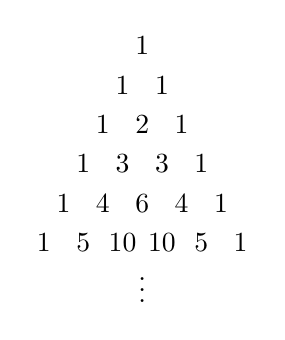
\begin{tikzpicture}[xscale=0.25,yscale=.5]
      \node (00) at ( 0, 0) {$1$};
      \node (10) at (-1,-1) {$1$};
      \node (11) at ( 1,-1) {$1$};
      \node (20) at (-2,-2) {$1$};
      \node (21) at ( 0,-2) {$2$};
      \node (22) at ( 2,-2) {$1$};
      \node (30) at (-3,-3) {$1$};
      \node (31) at (-1,-3) {$3$};
      \node (32) at ( 1,-3) {$3$};
      \node (33) at ( 3,-3) {$1$};
      \node (40) at (-4,-4) {$1$};
      \node (41) at (-2,-4) {$4$};
      \node (42) at ( 0,-4) {$6$};
      \node (43) at ( 2,-4) {$4$};
      \node (44) at ( 4,-4) {$1$};
      \node (50) at (-5,-5) {$1$};
      \node (51) at (-3,-5) {$5$};
      \node (52) at (-1,-5) {$10$};
      \node (53) at ( 1,-5) {$10$};
      \node (54) at ( 3,-5) {$5$};
      \node (55) at ( 5,-5) {$1$};
      \node (d1) at ( 0,-6) {$\vdots$};
    \end{tikzpicture}\\
    \noindent where each number is the sum of the two above, \eg $\binom42 = 6$.}
  \[
    \binom nk \defeq \frac{n!}{k!(n-k)!}.
  \]
  Find a formula for the number of $k$-cycle permutations of $A$
  using factorials and/or binomial coefficients.
\end{xca}

\section{The \texorpdfstring{$m$\th}{mᵗʰ} root:
  \coverings over the components of $\Cyc$}

Recall the equivalence $c : \Sc \we \Cyc_0$ of \cref{def:S1toC}
between the circle and the type of infinite cycles.
Here we set $\Cyc_0 \defeq \InfCyc$.

In this section, we reinterpret the degree $m$ function $\dg{m}$
as a map of infinite cycles. In fact it makes sense as a map on all cycles,
and we'll use it to begin the classification
of the connected \coverings on the components $\Cyc_n$,
of $\Cyc$, determined by the standard $n$-cycles, for positive integers $n$.
That's why it's instructive to rephrase connected \coverings over $\Sc$
in terms of cycles,
even though they could just be transported along the identity $\etop c:\Sc=\Cyc_0$ corresponding to $c$.

Before we do the degree $m$ maps, let's note that the
universal \covering over $\Cyc_0$ is represented by the constant function
$\cst{\pt_0}:\bn 1\to\Cyc_0$, sending the unique element
of $\bn 1$ to $\pt_0\defeq(\zet,\zs):\Cyc_0$, the standard infinite cycle.\footnote{%
  In light of \cref{lem:IdCisZet} we see that the fiber
  of this universal covering over $(X,t):\Cyc_0$ is (equivalent to) $X$ itself
  -- that's certainly a universal set associated to the
  infinite cycle $(X,t)$!}

For the rest of this section, we fix some positive $m:\NN$.
We now give a description of
the $m$-fold \covering over the circle in terms of cycles.

We proceed as follows.
First we present the answer, a \covering we call $\cdg{m}:\Cyc_0\to\Cyc_0$,
and then we prove that $\dg{m}:\Sc\to\Sc$ and $\cdg{m}:\Cyc_0\to\Cyc_0$
correspond to each other (and to $\pow{m}:\tilde R_m\to\Sc$)
under the equivalence $c:\Sc\we\Cyc_0$.

What should we require of $\cdg{m}(X,t)$ for $(X,t):\Cyc_0$?
Well, $\dg{m}:\Sc\to\Sc$ sends $\base$ to $\base$ and $\Sloop$ to $\Sloop^m$;
only the $\Sloop^k$ where $k$ is a multiple of $k$ is in the image of $\dg{m}$.
So we have to find an infinite cycle $(Y,u)$ with ``$u^m$ corresponding to $t$''.
We achieve this by ``streching'' $X$:
Let $Y$ be $m$ copies of $X$ and let $u$ jump idly from one copy to another except every $m$\th time when $u$ also is allowed to use $t$.
This is illustrated in \cref{fig:root} with the shift by $t$ being
vertical and the movement from copy to copy going around a circle.
\begin{marginfigure}
  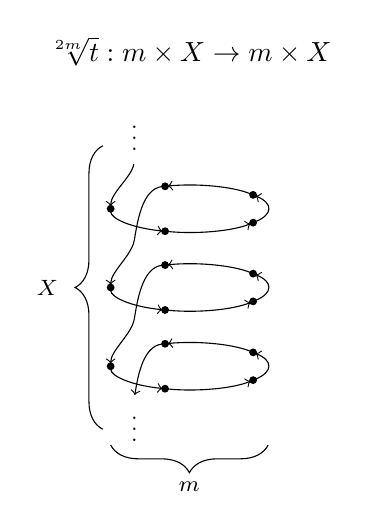
\begin{tikzpicture}
    \node (A) at (0,4) {$\sqrt[\uproot{2}m]t:{\bn m\times X}\to{\bn m\times X}$};
    \foreach \y in {0,1,2}
    { \begin{scope}[shift={(0,\y)}]
        \foreach \x in {0,...,4}
        { \node[fill,circle,inner sep=1pt] at (180+72*\x:1 and .3) {}; }
        \foreach \x in {0,...,3}
        { \draw[->,shorten <=1pt,shorten >=1pt]
          (180+72*\x:1 and .3) arc(180+72*\x:252+72*\x:1 and .3); }
      \end{scope} }
    \foreach \y in {1,2}
    { \begin{scope}[shift={(0,\y)}]
        \draw[->,shorten <=1pt,shorten >=1pt] (108:1 and .3)
        .. controls ++( 5:-.3) and ++(80:.2) .. (-.7,-.4)
        .. controls ++(80:-.2) and ++(90:.2) .. (-1,-1);
      \end{scope} }
    \draw[->,shorten <=1pt,shorten >=1pt] (108:1 and .3)
    .. controls ++( 5:-.3) and ++(80:.2) .. (-.7,-.4);
    \node (dz) at (-.7,-.7) {\footnotesize$\vdots$};
    \begin{scope}[shift={(0,3)}]
      \draw[->,shorten <=1pt,shorten >=1pt] (-.7,-.4)
      .. controls ++(80:-.2) and ++(90:.2) .. (-1,-1);
      \node (da) at (-.7,0) {\footnotesize$\vdots$};
    \end{scope}
    \draw [decorate,decoration={brace,amplitude=10pt}]
    (-1.1,-.8) -- (-1.1,2.8) node [black,midway,xshift=-20pt] {\footnotesize $X$};
    \draw [decorate,decoration={brace,amplitude=10pt}]
    (1,-1) -- (-1,-1) node [black,midway,yshift=-15pt] {\footnotesize $\bn{m}$};
  \end{tikzpicture}
  \caption{The $m$\th root $\sqrt[\uproot{2}m]t$
    of a function $t: X\to X$,
    here illustrated in the case $m=5$.}\label{fig:root}
\end{marginfigure}

\begin{construction}\label{con:root}
  For any type $X$ and $t:X\to X$, we define the $m$\th \emph{root}
  \[
    {\textstyle\sqrt[\uproot{2}m]t} : {\bn m\times X} \to {\bn m\times X}.
  \]
\end{construction}
\begin{implementation}{con:root}
  We set
  \[
    {\textstyle\sqrt[\uproot{2}m]t}(k,x)\defeq
    \begin{cases}
      (k+1,x)& \text{for $k<m-1$ and}\\
      (0,t(x))& \text{for $k=m-1$}.
    \end{cases}
  \]
\par \vspace{-1.5\baselineskip}
\qedhere
\end{implementation}
Only one $m$\th of the time does $\sqrt[\uproot{2}m]t$ use $t:X\to X$,
the rest of the time it applies the successor in $\bn m$.
Indeed, iterating $\sqrt[\uproot{2}m]t$
we get $(\sqrt[\uproot{2}m]t)^m(k,x)=(k,t(x))$;
hence the term ``$m$\th root'' is apt.

\begin{definition}
  The \emph{formal $m$\th root function} is defined by:
  \[
    \cdg{m}:\sum_{X:\UU}(X\to X)\to\sum_{X:\UU}(X\to X),\qquad
    \cdg{m}(X,t)\defeq(\bn m\times X,{\textstyle\sqrt[\uproot{2}m]t}).\qedhere
  \]
\end{definition}
\noindent We use $\rho$ for ``root'' to denote this incarnation
of the degree $m$ function.

\begin{lemma}\label{lem:root-pres-equiv}
  If $t:X\to X$ is an equivalence,
  then so is $\sqrt[\uproot{2}m]t : \bn m\times X \to \bn m\times X$.
\end{lemma}
\begin{proof}
  On one hand, an element in  $(\sqrt[\uproot{2}m]t)(\ell,y) = (0,x)$ consists
  of the assertion that  $\ell=m-1$ and an element in $t(y)=x$,
  so  $(\sqrt[\uproot{2}m]t)^{-1}(0,x)$ is equivalent
  to $t^{-1}(x)$, which is contractible if $t$ is an equivalence.

  On the other, if $k:\bn m$ is not $0$,
  then an element in $(\sqrt[\uproot{2}m]t)(\ell,y)=(k,x)$
  consists of the assertion that $\ell+1=k$ and an element in $y=x$,
  and so $(\sqrt[\uproot{2}m]t)^{-1}(k,x)$ is equivalent
  to the contractible type $\sum_{y:X}y=x$.\marginnote{%
    Of course, it's also quite easy to write down an inverse
    of $\sqrt[\uproot{2}m]{t}$ given an inverse of $t$.}
\end{proof}

\begin{lemma}
  If $(X,t)$ is a cycle, then so is $\cdg{m}(X,t)$.
\end{lemma}
\begin{proof}
  Clearly, $\bn m\times X$ is \nonempty if $X$ is.
  And we already know $\sqrt[\uproot{2}m]{t}$ is an equivalence if $t$ is.

  Suppose $(k,x),(k',x'):\bn m\times X$.
  We need to show the proposition that there exists $n:\zet$
  with $(k',x') = \bigl(\sqrt[\uproot{2}m]t\bigr)^n(k,x)$.
  Let $n:\zet$ be such that $x' = t^n(x)$.
  Then $(\sqrt[\uproot{2}m]t)^{nm}(k,x) = (k,t^n(x)) = (k,x')$,
  so if $k=k'$ we're done.
  Assume $k<k'$. Then $(\sqrt[\uproot{2}m]t)^{k'-k}(k,x') = (k',x')$,
  so $(\sqrt[\uproot{2}m]t)^{nm+k'-k}(k,x) = (k',x')$, as desired.
  The case $k>k'$ is similar.
\end{proof}

The question now arises: how does $\cdg{m}$ act on the components of $\Cyc$,
and what can we say about the preimages $\cdg{m}^{-1}(X,t)$
for an arbitrary cycle $(X,t)$?

The first part is easy, since the product of $\bn m$ with an $n$-element set
is an $mn$-element set. We set $\pt_n \defeq (\bn n,\zs) : \Cyc_n$.
\begin{lemma}
  The degree $m$ function restricts to give pointed maps
  \[
    \cdg{m} : \Cyc_n \ptdto \Cyc_{mn} \quad\text{and}\quad
    \cdg{m} : \Cyc_0 \ptdto \Cyc_0.
  \]
\end{lemma}
\begin{proof}
  Note\marginnote{%
    In terms of iterated addition, we have
    $\varphi(k,r) = (z \mapsto z+m)^r(k)$.}
  that the function $\varphi : (\bn m\times \zet) \to \zet$
  given by $\varphi(k,r)=k+mr$ is an equivalence,
  with inverse given by Euclidean division by $m$.
  Moreover, we have ${\varphi\!\sqrt[\uproot{2}m]\zs} = {\zs\varphi}$, since
  \[
    \varphi\bigl(\!\sqrt[\uproot{2}m]\zs(k,r)\bigr)
    = k+1+mr = \zs(\varphi(k,r))
    \quad\text{for all $(k,r):\bn m\times \zet$}.
  \]
  This shows that $\varphi$ gives an identification of infinite cycles
  $(\bn m\times\zet, \sqrt[\uproot{2}m]\zs) = (\zet,\zs)$,
  and hence the $m$\th root construction maps the component $\Cyc_0$ to itself.

  Analogously, we can restrict $\varphi$ to
  an equivalence $\bn m \times \bn n \we \sum_{k:\NN}(k<mn)$,
  and get an identification of cycles $\cdg{m}(\pt_n) = \pt_{mn}$,
  showing that $\cdg{m}$ maps the component $\Cyc_n$ to the component $\Cyc_{mn}$.
\end{proof}

We now analyze how $\cdg{m}$ acts on paths.
Let $\pathpair{\etop{e}}{!}:(X,t)=(X',t')$.
Since $\cdg{m}$ maps first components $X$ to $\bn m\times X$, we get that
the first projection of $\ap{\cdg{m}}\pathpair{\etop{e}}{!}$ is
$\overetop{\id\times e} : (\bn m\times X) = (\bn m\times X')$.
We are particularly interested in the case of the loops,
that is, $\pathpair{\etop{e}}{!}:(X,t)=(X,t)$.
We calculate $(\id\times e)(k,x) = (k,e(x))$,
which by the property of the $m$\th root is equal to $(\sqrt[\uproot{2}m]e)^m(k,x)$.
In particular, if we take $e\defeq t^{-1}$,
then we get $(\id\times t^{-1}) = (\sqrt[\uproot{2}m]{t^{-1}})^m$, which means that
$\ap{\cdg{m}}\pathpair{\etop{t}^{-1}}{!}$ is indeed the $m$\th power of a
generating loop at the image cycle $\cdg{m}(X,t)$.
In particular, this holds for the standard infinite cycle $(\zet,\zs):\Cyc_0$
and the standard $n$-cycle $(\bn n,\zs):\Cyc_n$.

Why does $\cdg{m}:\Cyc_0\to\Cyc_0$
correspond to the $m$-fold \covering we defined in \cref{def:mfoldS1cover}?
This is encapsulated by the fact that under the equivalence $c:\Sc\to C$, the two $m$-fold covers agree in the sense that the two functions given as composites in
\[
  \begin{tikzcd}
    \Sc\ar[r,"c"]\ar[d,"\dg{m}"'] & \Cyc_0\ar[d,"\cdg{m}"] \\
    \Sc\ar[r,"c"] & \Cyc_0
  \end{tikzcd}
\]
are equal; we need an element in
\[
  \cdg{m}c=_{\Sc\to\Cyc_0}c\,\dg{m}.
\]
Under the equivalence
\[
  \ev_{\Cyc_0}:(\Sc\to\Cyc_0)\we \sum_{(X,t):\Cyc_0}\bigl((X,t)=(X,t)\bigr)
\]
of \cref{lem:freeloopspace},
the composite $c\,\dg{m}$ is given by $\bigl((\zet,\zs),\zs^{-m}\bigr)$
and the composite $\cdg{m}c$ is given by
$\bigl((\bn m\times\zet,\sqrt[\uproot{2}m]{\zs}),\id\times\zs^{-1}\bigr)$:
we must produce an element in
\[
  \Bigl((\bn m\times\zet,\sqrt[\uproot{2}m]{\zs}),\id\times\zs^{-1}\Bigr)
  = \bigl((\zet,\zs),\zs^{-m}\bigr).
\]
Consider the equivalence  $\varphi: (\bn m\times \zet)\to\zet$ with $\varphi(k,n)=k+mn$ discussed above.
Transport of $\sqrt[\uproot{2}m]\zs$ along $\varphi$ is exactly $\zs$.
(I.e., $\varphi\!\sqrt[\uproot{2}m]\zs=\zs\varphi$;
note the way we formulate this so that we don't need to talk about the inverse of $\varphi$\footnote{%
  Of course, the inverse of $\varphi$ maps $z:\zet$ to the remainder and the integer quotient of $z$ under Euclidean division by $m$, cf.~\cref{lem:euclid-div}.}.)
Likewise, transport of $\id\times\zs^{-1}$ along $\varphi$ is $\zs^{-m}$,
so that $\varphi$ lifts to an element in
$\bigl((\bn m\times\zet,\sqrt[\uproot{2}m]{\zs}), \id\times\zs^{-1}\bigr)
= \bigl((\zet,\zs),\zs^{-m}\bigr)$.

\begin{xca}\label{xca:pointed-maps-circle}
Verify $\cdg{m}c=_{\Sc\ptdto\Cyc_0}c\,\dg{m}$ in case all maps are taken to be pointed.
\end{xca}

So we know that the fiber of $\cdg{m}$ at an infinite cycle $(X,t)$
is an $m$-element set. In fact, we can identify this set as
$X/m \defeq X/\sim_m$ where $\sim_m$ is the equivalence relation that
identifies points that are a distance $mr$ apart, for some $r:\zet$.
Formally, let $x\sim_m x'$ if and only if $\exists_{r:\zet}(x'=t^{mr}(x))$.
(Such an $r$ is unique if it exists.)
Indeed, the fiber is
\[
  \sum_{(Y,u):\Cyc_0}\bigl((X,t) = (\bn m\times Y, \sqrt[\uproot{2}m]{u})\bigr).
\]
The equivalence is obtained by sending an equivalence class $Y$ of $X/m$ to
the corresponding infinite cycle $(Y,u^m)$ together with the
natural identification $(X,t) = (\bn m\times Y, \sqrt[\uproot{2}m]{u^m})$.
See \cref{thm:fiber-cdg} below for a careful proof of a more general statement.

The reader will no doubt have noticed that $X/m$ is a \emph{finite cycle}.
We'll return to the significance of this below in~\cref{sec:higher-images}.

Our next step is to identify the fiber of $\cdg{m}$ over a general cycle $(X,t)$.
Classically, the remaining cases are those of finite $n$-cycles,
but it's illuminating to be a bit more general.
Note that the equivalence relation $\sim_m$ defined above for an infinite cycle
makes sense for all cycles.

\begin{lemma}\label{lem:sum-cycle-point-contr}
  For any order $d:\Order$, the type $\sum_{(X,t):\Cyc_d}X$ is contractible,
  where $\Cyc_d$ denotes the component of $\Cyc$ consisting
  of cycles of order $d$.
\end{lemma}
\begin{proof}
  This is relatively straight-forward from \cref{lem:IdCycle}.
  The type in question is nonempty since all cycles have a nonempty underlying set,
  so it suffices to prove the type is a proposition.
  So let $(X,t),(X',t')$ be cycles of order $o$, and take $x:X$ and $x':X$.
  An identification $((X,t),x) = ((X',t'),x')$ is given by an equivalence of
  cycles $e : (X,t)=(X',t')$ with $e(x)=x'$.
  But evaluation at $x$ induces an equivalence
  $\bigl((X,t)=(X',t')\bigr) \simeq X'$,
  so there exists a unique $e$ with $e(x)=x'$.
\end{proof}
\begin{lemma}\label{lem:m-root-id}
  For any cycle $(X,t)$, if $(\sqrt[\uproot{2}m]{t})^n = \id$,
  then $m$ divides $n$, \ie $n=mq$ for some $q:\zet$, and $t^q=\id$.
  In other words, $m$ divides the order of $\sqrt[\uproot{2}m]{t}$.
\end{lemma}
This follows simply by looking at the first component,
where $\sqrt[\uproot{2}m]{t}$ acts as the successor operation on $\bn m$.

We're almost ready to identify the fiber of $\cdg{m}$ at a cycle $(X,t)$.
We know from \cref{lem:m-root-id} that the fiber
is \nonempty only if $m$ divides the order of $t$.
A key ingredient for the converse is the following.
\begin{lemma}\label{lem:X-mod-m-chosen}
  Let $(X,t):\Cyc$ be a cycle with a chosen point $x_0:X$
  and with order divisible by $m$.
  Then the map $f : \bn m \to X/m$, $f(k) \defeq [t^k(x_0)]$
  is an equivalence.
\end{lemma}
\begin{proof}
  Fix an equivalence class $V:X/m$ and consider its preimage under $f$,
  $f^{-1}(V) \jdeq \sum_{k:\bn m}(V=[t^k(x_0)])$.
  The contractibility of this type is a proposition, so we may choose
  $x:X$ with $V=[x]$.
  Then $(V=[t^k(x_0)])\equiv([x]=[t^k(x_0)])\equiv(x\sim_m t^k(x_0))$.
  So we need to show that $\sum_{k:\bn m}(x\sim_m t^k(x_0))$ is contractible.
  More simply, we need to show that there is a unique $k$ with $x\sim_m t^k(x_0)$.
  Since $(X,t)$ is a cycle, we may further choose $n:\zet$ with $x=t^n(x_0)$.
  By Euclidean division, write $n=qm+r$ with $q:\zet$, $r:\bn m$.
  Then $x = t^n(x_0) \sim_m t^r(x_0)$, so we have our center.
  Let $k:\bn m$ also satisfy $x\sim_m t^k(x_0)$.
  We need to show the proposition $k=r$.
  But $t^{r-k}(x_0) \sim_m x_0$, so we may take $q:\zet$ with $t^{qm+r-k}(x_0)=x_0$.
  Since $m$ divides the order of $t$, this implies $r=k$, as desired.
\end{proof}
Now we have all the pieces needed to prove the main result.
\begin{theorem}\label{thm:fiber-cdg}
  For \emph{any} cycle $(X,t)$, the preimage $\cdg{m}^{-1}(X,t)$
  is equivalent to $P\times X/m$,
  where $P\defeq (m \mid \ord(t)) \jdeq (H_t \subseteq m\zet)$
  expresses that $m$ divides the order of $t$.
\end{theorem}
\begin{proof}
  We'll use \cref{lem:weq-iso}, and we first define the function
  \[
    g : \cdg{m}^{-1}(X,t) \to P\times X/m,
  \]
  by mapping $(Y,u)$ and an identification of cycles
  $e : (X,t) = (\bn m\times Y,\sqrt[\uproot{2}m]{u})$
  to the proof of $P$ from \cref{lem:m-root-id}
  and the class $V_e\defeq [e^{-1}(0,y)]:X/m$, for any $y:Y$.
  Note that this doesn't depend on $y$, so that \cref{thm:wconstant-elim} applies.
  As a subset of $X$, $V_e=\setof{x:X}{\fst(e(x))=0}$.

  In the other direction, to define the function
  \[
    h : P\times X/m \to \cdg{m}^{-1}(X,t),
  \]
  fix an equivalence class $V:X/m$,
  and assume that $m$ divides the order of $t$.
  Then we have, with a bit of abuse of notation, the cycle $(V,t^m)$,
  where we also write $V$ for the type of elements in $X$ that lie in the class $V$,
  and $t^m$ is the restriction of this power of $t$ to $V$.\footnote{%
    If $x$ lies in $V$, then so does $t^m(x)$.}
  We also need an identification
  $(X,t)=(\bn m\times V,\sqrt[\uproot{2}m]{t^m})$.
  This we define via a map $e : \bn m\times V \to X$, $e(k,x) \defeq t^k(x)$.
  This is an equivalence as long as the orders match.
  So let $n:\zet$, and assume first that $t^n=\id$.
  Then $P$ implies that we may write $n=qm$ for some $q:\zet$,
  so
  \[
    (\sqrt[\uproot{2}m]{t^m})^n
    = (\sqrt[\uproot{2}m]{t^m})^{qm}
    = (\id \times t^m)^q = (\id \times t^{qm}) = \id.
  \]
  Conversely, we know from \cref{lem:m-root-id} again,
  that if $(\sqrt[\uproot{2}m]{t^m})^n=\id$,
  then we may write $n=qm$ for some $q:\zet$,
  and $(t^m)^q=\id$, which by \cref{lem:cycle-order-point-ap}
  implies that $t^n = \id$.

  Straight from these definitions, we see that $g\circ h=\id$.
  We leave to the reader to check that $h\circ g=\id$.
\end{proof}

\section{Higher images}
\label{sec:higher-images}

In this section we take a quick break from characterizing the connected \coverings
of $\Cyc_n$ for finite orders $n$ in order to make good on our earlier promise
to say something about the fact that the fiber of $\cdg{m}$, $X/m$, at a cycle $(X,t)$
of order divisible by $m$, itself carries a cycle structure.
This involves the notion of $0$-image of a map, but we might as well introduce the general
notion of $n$-image while we're at it.

Recall from \cref{def:prop-image} the propositional image of a map $f : A \to B$,
  \[
    \im(f) \jdeq \sum_{y:B}\exists_{x:A}(y \eqto f\,x)
           \jdeq \sum_{y:B}\Trunc{\sum_{x:A}(y \eqto f\,x)}
           \jdeq \sum_{y:B}\Trunc{\inv f (y)}.
  \]
We now generalize the propositional image
to higher images, replacing the propositional
truncation involved in the definition by $n$-truncation.

Recall furthermore the image factorization from \cref{xca:unique-fact-image}:
  \[
    \begin{tikzcd}
      A \ar[rr,"f"]\ar[dr,"p"'] & & B \\
      & \im(f)\ar[ur,"i"'] &
    \end{tikzcd}
  \]
Here $p$ is surjective and $i$ is injective, and any such factorization is equivalent to this one. Both surjectivity
(\cref{def:surjection}) and injectivity (\cref{def:injection})
rely on the notion of proposition: all fibers of $p$ are nonempty
and all fibers of $i$ are propositions.

The uniqueness of the factorization $f=ip$ can be visualized
in terms of the two diagonals of the diamond below:
for any surjection $g$ and injection $h$ such that $f=hg$,
that is, the diagram below on the left commutes,
one can construct a (unique) equivalence $e$ such that
the diagram on the right commutes.

\begin{equation}\label{eqn:image-univ-prop}
    \begin{tikzcd}
      & X \ar[dr,"h"] & & & X \ar[dr,"h"] &\\
      A \ar[rr,"f"]\ar[dr,"p"'] \ar[ur,"g"]& & B
&
      A \ar[dr,"p"'] \ar[ur,"g"]& & B  \\
      & \im(f)\ar[ur,"i"'] & & & \im(f)\ar[ur,"i"']\ar[uu, dotted, "e"] &
    \end{tikzcd}
\end{equation}

The existence of a unique equivalence $e$ as above is called the
\emph{universal property of the propositional image}.
Uniqueness of $e$ above also follows from the following two exercises.

\begin{xca}\label{xca:cancel-injection}
Let $A,B,X$ be types and $i:A\to B$ an injection.
Let $i\blank : (X\to A) \to (X\to B)$ be postcomposition with $i$.
Show that $\ap{i\blank}: (f = g) \to (if = ig)$ is an equivalence,
for any $f,g: X\to A$.
\end{xca}
\begin{xca}\label{xca:cancel-surjection}
Let $A,B,Y$ be types and $p:A\to B$ be a surjection.
Let $\blank p : (B\to Y) \to (A\to Y)$ be precomposition with $p$.
Show that $\ap{\blank p}: (f = g) \to (fp = gp)$ is an equivalence,
for any $f,g: B\to Y$.
\end{xca}

We will now define higher images and generalize the notions
of injection and surjection such that a similar
universal property of higher images can be proved.

\begin{definition}\label{def:n-image}
  Let $A,B$ be types and let $f : A \to B$. We define the $n$-\emph{image} of $f$ as
  \glossary(iman){$\protect\im_n(f)$}{the $\protect n$-image of $\protect f$}
  \[
    \im_n(f) \defeq \sum_{b:B}\Trunc{\inv f (b)}_n.\qedhere
  \]
\end{definition}

Observe that $\im_{-1}(f) \jdeq \im(f)$.

\begin{definition}\label{def:n-connected}
  A type $A$ is called $n$-\emph{connected}\index{type!$n$-connected}
  if its truncation $\Trunc A _ n$ is contractible.

  A function $f : A \to B$ is called $n$-\emph{connected}\index{function!$n$-connected}
  if the fiber $\inv f (b)$ is $n$-connected, for each $b:B$.
\end{definition}

Thus, any type is $(-2)$-connected, since its $(-2)$-truncation is contractible.
Moreover, the $(-1)$-connected types are precisely the nonempty ones,
and the $0$-connected types are those we have called connected in \cref{def:connected}.

\begin{definition}\label{def:n-truncated}
  A function $f : A \to B$ is called $n$-\emph{truncated}\index{function!$n$-truncated}
  if the fiber $\inv f (b)$ is an $n$-type, for each $b:B$.
\end{definition}

One may verify now that the $(-1)$-connected functions are the surjections, and
the $(-1)$-truncated functions are the injections.

There is a \emph{factorization} $f = i p$ of a map $f : A \to B$ through its $n$-image,
where $p$ is defined by setting $p(a)\defeq (f(a),\trunc{(a,\refl{f(a)})}_n)$,
and where $i$ is defined by setting $i\defeq\fst$, as in the following diagram.

\begin{equation}\label{eqn:n-image-factorization}
    \begin{tikzcd}
      A \ar[rr,"f"]\ar[dr,"p"'] & & B \\
      & \im_n(f)\ar[ur,"i"'] &
    \end{tikzcd}
\end{equation}

The map $i$ is $n$-truncated, because, for any $b:B$, the fiber $\inv i (b)$ is equivalent to $\Trunc{\inv f (b)}_n$.
Furthermore, by \cref{lem:sum-of-fibers} and the following lemma, $p$ is $n$-connected.

\begin{lemma}\label{lem:trunc-n-connected}
For every type $A$, the constructor $\trunc{\blank}_n : A\to \Trunc{A}_n$
is $n$-connected.
\end{lemma}
\begin{proof}
We have to prove that the $n$-truncation of each fiber of $\trunc{\blank}_n$
is contractible. We start by defining a function
$c:\prod_{x:\Trunc{A}_n} \Trunc{\inv{\trunc{x}}_n}_n$ producing the centers.
Since $c$ takes values in $n$-types, we can define $c$ by
$n$-truncation elimination by setting
$c(\trunc{a}_n) \defeq \trunc{(a,\refl{\trunc{a}_n})}_n$.

The next step is to construct an element of
$\prod_{x:\Trunc{A}_n} \prod_{y:\Trunc{\inv{\trunc{x}}_n}_n} (c(x)=y)$.
Since the identity $c(x)=y$ is an $(n-1)$-type, it suffices to give an element of
$\prod_{x:\Trunc{A}_n} \prod_{z:\inv{\trunc{x}}_n} (c(x)=\trunc{z}_n)$.
Since fibers are sum types,  it suffices to give an element of
$\prod_{x:\Trunc{A}_n} \prod_{a:A} \prod_{p: x=\trunc{a}_n} (c(x)=\trunc{(a,p)}_n)$.
After swapping the first two products, the identity reduces by path induction
to $c(\trunc{a}_n)=\trunc{(a,\refl{\trunc{a}_n})}_n$, for which we can use
the reflexivity path.
\end{proof}

\begin{construction}\label{con:fibcomp=fibfib}
  Let $g:A\to X$ and $h: X\to B$, and let
$\tilde{g}:A\to \sum_{b:B}\inv h (b)$ be the composition of $g$
with the canonical equivalence $X\to \sum_{b:B}\inv h (b)$ from \cref{lem:sum-of-fibers}.
Thus $\tilde{g}(a)\jdeq (h(g(a)),g(a),\refl{h(g(a))})$ for each $a:A$,
and we have the following commutative diagram:
  \[
    \begin{tikzcd}
      A \ar[r,"g"] \ar[dr,"\tilde{g}"'] & X \ar[r,"h"] \ar[d, eqr] & B \\
      & \sum_{b:B}\inv h (b) \ar[ur,"\fst"'] &
    \end{tikzcd}
  \]
Then we have equivalences $e(b) : \inv {(hg)} (b) \equivto \sum_{y:\inv h (b)} \inv {\tilde{g}}(b,y)$
for all $b:B$.
\end{construction}
\begin{implementation}{con:fibcomp=fibfib}
Let, for each $b:B$, $e(b)$ map any pair $(a,p):\inv {(hg)} (b)$ to
$((g(a),p),(a,q))$. Here $q$ is of type $(b,g(a),p) = (h(g(a)),g(a),\refl{h(g(a))})$
and is given componentwise by $p: b=h(g(a))$, $\refl{g(a)}$, and by the
easy path over $p$ from $p$ to $\refl{h(g(a))}$ in the identity type family $\blank=h(g(a))$.
This construction uses \cref{def:pairtopath}, \cref{def:pathover-trp},
and \cref{xca:trp-in-a/x=b/x}\ref{trp-in-x=a}.
\end{implementation}

\begin{xca}\label{xca:fibcomp=fibfib}
Complete the details of \cref{con:fibcomp=fibfib}.
In particular, prove that $e$ is a fiberwise equivalence.
Alternatively, construct your own $e$ by using \cref{cor:contract-away} (twice!).
\end{xca}

\begin{xca}\label{xca:pullout-base-type}
Let $X$ be an $n$-type and let $Y(x)$ be a type for all $x:X$.
Construct canonical equivalences
$\Trunc{\sum_{x:X} Y(x)}_n \to \sum_{x:X} \Trunc{Y(x)}_n$  and
$\Trunc{\prod_{x:X} Y(x)}_n \to \prod_{x:X} \Trunc{Y(x)}_n$.
\end{xca}

We shall now show that the $n$-image factorization
of $f:A\to B$ in \cref{eqn:n-image-factorization} is unique.
This result can be visualized in a similar way as we
did in \cref{eqn:image-univ-prop} for $n=-1$,
and is called the \emph{universal property of the $n$-image}.

\begin{marginfigure}
\noindent\begin{tikzcd}
      & X \ar[dr,"h"] & \\
      A \ar[rr,pos=0.7,"f"]\ar[dr,"p"'] \ar[ur,"g"]& & B\\
      & \im_n(f)\ar[ur,"i"']\ar[uu,dotted,pos=0.3, "e"] &
    \end{tikzcd}
\caption{Universal property of the $n$-image.}
\label{fig:n-image-univ-prop}
\end{marginfigure}

\begin{theorem}\label{thm:n-im-univ-prop}
Let conditions be as in \cref{eqn:n-image-factorization}.
For a given type $X$, assume we are given an $n$-connected
function $g:A\to X$ and an $n$-truncated function $h:X\to B$ with $f=hg$.
Then there exists a unique equivalence $e: \im_n(f)\to X$
such that $g=ep$ and $i=he$.
\end{theorem}

\begin{proof}
We have to construct the equivalence $e$ such that the diagram
in \cref{fig:n-image-univ-prop} commutes; uniqueness of $e$
follows from an easy generalization of \cref{xca:cancel-injection}
and the left triangle in \cref{fig:n-image-univ-prop}.
To simplify this construction,
we are going to replace $g$ and $h$ by projection maps.

In view of \cref{con:fibcomp=fibfib}, we may assume without
loss of generality that $X\jdeq \sum_{b:B} P(b)$ for some
family of $n$-types $P(b)$, and $h\jdeq\fst$.

\begin{marginfigure}
  \noindent\begin{tikzcd}[column sep=tiny]
      &\sum\limits_{b:B} P(b)\ar[rd,"\fst"]\\
      \sum\limits_{b:B} R(b)
        \ar[rd,"{(b,y,q)\mapsto(b,\trunc{(y,q)}_n)}"']
        \ar [ru,"{(b,y,q)\mapsto(b,y)}"]
        \ar [rr,pos=0.7,"\fst"]
      &&B\\
      &\sum\limits_{b:B} \Trunc{R(b)}_n
         \ar [ru,"\fst"']
         \ar [uu,dotted,pos=0.3,"e"']
\end{tikzcd}
\caption{Universal property of the $n$-image, reinterpreted.}
\label{fig:n-im-univ-prop-sumB}
\end{marginfigure}

By \cref{lem:sum-of-fibers} we may also assume without
loss of generality that
$A\jdeq\sum_{b:B}\sum_{y:P(b)} Q(b,y)$, where
$Q(b,y) \defeq\inv g (b,y)$ are the fibers of $g$,
which are all $n$-connected by assumption.
Define $R(b)\defeq\sum_{y:P(b)} Q(b,y)$ for all $b:B$.
With $A\jdeq \sum_{b:B} R(b)$, the function $g$
takes the form of the projection map $(b,y,q)\mapsto(b,y)$,
as shown in \cref{fig:n-im-univ-prop-sumB}.
By $f=hg$ we then get that $f$ is the first projection,
with its $n$-image equivalent to $\sum_{b:B} \Trunc{R(b)}_n$.
The $n$-connected map $p$ then takes the form
$(b,y,q)\mapsto(b,\trunc{(y,q)}_n)$ as shown in
\cref{fig:n-im-univ-prop-sumB}.

Since $B=\sum_{b:B}\bn{1}$, each type in \cref{fig:n-im-univ-prop-sumB}
can be considered to be the sum of a type family parametrized by $b:B$.
For constructing the equivalence $e$ that makes
\cref{fig:n-im-univ-prop-sumB} commute, it suffices to
construct for each $b:B$ the equivalence $e_b$ such that
\cref{fig:n-im-univ-prop-b:B} commutes.
Then we obtain $e$ as desired by summing over $B$, that is,
by putting $e(b,z) \defeq (b,e_b(z))$ for all $b:B$ and $z:\Trunc{R(b)}_n$.

\begin{marginfigure}
  \noindent\begin{tikzcd}
      &P(b)\ar[rd]\\
      R(b)
        \ar[rd,"{\trunc{\blank}_n}"']
        \ar [ru,"{\fst}"]
      &&\bn{1}\\
      &\Trunc{R(b)}_n
         \ar [ru]
         \ar [uu,dotted,"e_b"']
\end{tikzcd}
\caption{Taking summands for $b:B$ in \cref{fig:n-im-univ-prop-sumB}.}
\label{fig:n-im-univ-prop-b:B}
\end{marginfigure}

Now let $b:B$. We have $\Trunc{R(b)}_n \jdeq \Trunc{\sum_{y:P(b)} Q(b,y)}_n$.
By \cref{xca:pullout-base-type}, since $P(b)$ is an $n$-type by assumption,
we have the canonical equivalence
$\Trunc{\sum_{y:P(b)} Q(b,y)}_n\to\sum_{y:P(b)}\Trunc{Q(b,y)}_n$
defined by mapping $\trunc{(y,q)}_n$ to $(y,\trunc{q}_n)$.
For each $y:P(b)$, since $Q(y,b)$ is by assumption $n$-connected,
so that $\Trunc{Q(b,y)}_n = \bn{1}$,
we also have the canonical equivalence $\fst: \sum_{y:P(b)}\Trunc{Q(b,y)}_n \to P(b)$.
The composite of these two equivalences is $e_b$. Regarding the commutation
of \cref{fig:n-im-univ-prop-b:B}, we have $e_b \trunc{\blank}_n \jdeq \fst$
for the left triangle, and the right triangle commutes trivially.

An alternative proof of the uniqueness of $e$ can be obtained
by using the right triangle in \cref{fig:n-im-univ-prop-sumB}.
This reduces the uniqueness of $e$ to the uniqueness of $e_b$
for each $b:B$. The latter follows from the universal property
of $n$-truncation and the left triangle in \cref{fig:n-im-univ-prop-b:B}.
\end{proof}

As an application, we consider the fibers of $m$\th root map
$\cdg{m}$. On infinite cycles, this is equivalent to the degree $m$ map
of the circle by~\cref{xca:pointed-maps-circle}, so we have a map
$\blank/m : \Cyc_0 \to \Set$, which we can identify with the family
$R_m : \Sc \to \Set$ (\cref{def:RmtoS1})
after precomposition with the equivalence
$c : \Sc \to \Cyc_0$ from~\cref{thm:S1bysymmetries}.
For every infinite cycle $(X,t)$, the set $X/m$ has $m$ elements,
so the $(-1)$-image is $\FinSet_m$, the groupoid of $m$-element sets
(\cref{def:groupoidFin}).
But what is the $0$-image?

\begin{theorem}\label{thm:image-Z-to-Cm}
  The $0$-image factorization of the map $\blank/m : \Cyc_0 \to \Set$
  is the composition $p\circ q$, where $q : \Cyc_0 \to \Cyc_m$
  sends the infinite cycle $(X,t)$ to the $m$-cycle $(X/m,\bar t)$,
  where $\bar t : X/m \to X/m$ maps $[x]$ to $[t(x)]$,
  and $p:\Cyc_m\to\Set$ sends an $m$-cycle to its underlying set.
\end{theorem}

\begin{proof}
  We need to check that $q$ is $0$-connected
  and that $p$ is $0$-truncated.

  The latter is direct, since the preimage of $p$ at an $m$-element set $Y$
  is the set of functions $u : Y \to Y$ that make $Y$ into an $m$-cycle.

  To show that $q$ is $0$-connected,
  it suffices to consider the fiber at the standard $m$-cycle $(\bn m,\zs)$.
  We'll show that this fiber is equivalent to $\Cyc_0$ itself, which is indeed $0$-connected.
  The mediating map is induced by our old friend $\cdg{m}$.
  Indeed, define $\varphi : \Cyc_0 \to q^{-1}(\bn m,\zs)$
  by $\varphi(X,t)\defis(\cdg{m}(X,t), r)$,
  where $r$ is the canonical equivalence $(\bn m\times X)/m \equivto \bn m$.
  The inverse of $\varphi$, $\psi$, sends a pair $((Y,u), r)$,
  with $(Y,u):\Cyc_0$ and $r : Y/m \equivto \bn m$
  to $(r^{-1}(0), u^m)$.
\end{proof}

\begin{xca}
  Complete the proof by verifying that $\varphi$ and $\psi$ are indeed mutually inverse.
\end{xca}

The theorem and its proof in fact generalize to all orders.

\begin{xca}\label{xca:image-Cmd-to-Cm}
  Let $d$ be any order and consider the fiber of $\cdg{m}$ on the component
  $\Cyc_{md}$, $\blank/m : \Cyc_{md} \to \Set$.
  Show that the $0$-image factorization of this goes via $\Cyc_m$ by
  lifting $\blank/m$ to $q : \Cyc_{md} \to \Cyc_m$.
  In particular, show that the preimage of $q$ at the standard $m$-cycle
  is equivalent to $\Cyc_d$.
\end{xca}

\section{Universal property of $\Cyc_n$}
\label{sec:universal-property-cyc-n}

This section is devoted to showing that maps out of $\Cyc_n$ into a groupoid $A$
are equivalently given by the choice of a point together with a symmetry of
order $n$: that is any map $\Cyc_n \to A$ is fully determined by a point $a$ together with a symmetry $\sigma:a\eqto a$ such that
$\sigma^n=\refl a$.\footnote{Notice that this is a less general result than the universal property of the circle, or equivalently, the case $n=0$, where we don't need to assume that $A$ is a groupoid.}

Recall that $\Cyc_n$ contains the point $\pt_n \defequi (\bn n, \zs)$,
\ie the standard $n$-cycle. This
point has a symmetry $\sigma_n \defequi (\inv\zs, !)$ whose second projection is a
proof that $\zs\inv\zs = \inv\zs\zs$.
%
Recall also from \cref{cor:id-m-cycle} that all elements of $\pt_n = \pt_n$ are
of the form $\sigma_n^i$ for $i=0,\dots,n-1$.

Given a groupoid $A$, and a map $f :
\Cyc_n \to A$, one can consider $f(\pt_n):A$ and $\ap f (\sigma_n): f(\pt_n) =
f(\pt_n)$. The equation $\refl {\pt_n} = \sigma_n^n$ in
$\Cyc_n$ is mapped by $f$ to a proof of $\refl {f(\pt_n)} =
\ap f(\sigma_n)^n$. Hence, the following map is well-defined:
\begin{displaymath}
  \ev_{n,A} : (\Cyc_n \to A) \to \sum_{a:A}\sum_{\sigma:a\eqto a}\refl a = \sigma^n,\quad
  f \mapsto (f(\pt_n), \ap f (\sigma_n), !)
\end{displaymath}

\begin{theorem}
  For any groupoid $A$, the map $\ev_{n,A}$ is an equivalence.
  \label{prop:ump-cycn-into-groupoids}
\end{theorem}
\begin{proof}
  Let $a:A$ and $\sigma:a\eqto a$ be such that $\refl a = \sigma^n$ holds.
  We want to prove that the fiber
  \begin{displaymath}
    \sum_{f:\Cyc_n \to A} (a,\sigma, !) \eqto \ev_{n,A}(f)
  \end{displaymath}
  is contractible. Hence we first need to craft a function $f:\Cyc_n \to A$
  together with $p:a\eqto f(\pt_n)$ such that $\ap f (\sigma_n) \cdot p = p
  \cdot \sigma$.

  In order to do so, we will craft a function $f:\Cyc_n \to A$ together with a
  function $\hat p_x: \pt_n \eqto x \to a \eqto f(x)$ for each $x:\Cyc_n$ such that
  $\hat p_x(\blank\sigma_n) = \hat p_x(\blank) \sigma$. By setting $p \jdeq \hat
  p_{\pt_n}(\refl {\pt_n})$, we would have succeeded. Indeed, path induction on
  $\alpha: x \eqto x'$ shows that $\hat p_{x'}(\alpha \blank) = \ap f (\alpha) \hat
  p_x(\blank)$ on one hand, and the hyptohesis on $\hat p$ proves that $\hat
  p_{\pt_n} (\blank) \sigma = \hat p_{\pt_n}(\blank \sigma_n)$ on the other
  hand. This leads to the chain of equations:
  \begin{align*}
    p \sigma &= \hat p_{\pt_n}(\refl {\pt_n}) \sigma
               = \hat p_{\pt_n}(\refl {\pt_n}\sigma_n)
               = \hat p_{\pt_n}(\sigma_n\refl {\pt_n}) \\
             &= \ap f (\sigma_n) \hat p_{\pt_n}(\refl {\pt_n})
               = \ap f (\sigma_n) p
  \end{align*}

  It remains to craft the promised $f$ and $\hat p$. For each $x:\Cyc_n$, consider the type
  \begin{displaymath}
    T(x) \defequi \sum_{b:A}\sum_{\pi: \pt_n \eqto x \to a \eqto b}
    \pi(\blank\sigma_n) = \pi(\blank) \sigma
  \end{displaymath}
  We claim that $T(x)$ is contractible. To prove this proposition for $x$
  ranging over the connected type $\Cyc_n$, it is enough to only prove it for
  $x \jdeq \pt_n$. However, as $i \mapsto \sigma_n^i$ provides an equivalence
  $\bn n \to (\pt_n = \pt_n)$, we get:
  \begin{displaymath}
    T(\pt_n) \weq \sum_{b:A}\sum_{\pi: \bn n \to a \eqto b} \pi(\blank + 1) = \pi(\blank)\sigma
  \end{displaymath}
  Now, note that $\pi:\bn n \to a\eqto b$ such that $\pi(\blank +1) = \pi(\blank)
  \sigma$ is entirely determined by $\pi(0)$, as then $\pi(i) = \pi(0)\sigma^i$
  for all $i:\bn n$. Moreover, an element $q$ in $a\eqto b$ defines a function
  $\pi_q:i \mapsto q\sigma^i$ which satisfies the equation $\pi_q( \blank +1) =
  \pi_q(\blank)q$. In other words, we have an equivalence:
  \begin{displaymath}
    \left( \sum_{\pi:\bn n \to {a\eqto b}} \pi(\blank +1) = \pi(\blank )\sigma \right)
    \equivto
    (a \eqto b), \quad
    (\pi, !) \mapsto \pi(0).
  \end{displaymath}
  Hence, we can simplify further $T(\pt_n)$:
  \begin{displaymath}
    T(\pt_n) \weq \left(\sum_{b:A} a \eqto b\right) \weq 1
  \end{displaymath}
  We then get $f(x)$ by selecting a center of contraction for each $x:\Cyc_n$, and
  the function $\hat p_x$ is then defined as the first projection of the second
  component of this center of contraction.
  %
  \marginnote{The construction of $f$ is really an ad hoc version of the delooping of the abstract group morphism $\sigma_n^i \mapsto \sigma^i$. If we move this section forward, one can rewrite it as such.}


  Finally, we prove that the fiber $\inv{\ev_{n,A}}(a,\sigma,!)$ is a
  proposition. As we just proved that it is inhabited, we would have
  successfully shown that the fiber is contractible. Given two elements
  $(f,p,!)$ and $(f',p',!)$ of the fiber, we want to find a path between the
  two, that is $\chi:\prod_{x:\Cyc_n} f(x) \eqto f'(x)$ such that the following
  commutes:
  \begin{displaymath}
    \begin{tikzcd}
      a \rar[eqr,"p"] \dar[eql,"p'"'] & f(\pt_n) \dlar[eqr,"\chi(\pt_n)"]\\
      f'(\pt_n) &
    \end{tikzcd}
  \end{displaymath}
  Let us denote $U(x)\defequi f(x) \eqto f'(x)$ for $x:\Cyc_n$, and notice that
  these types are sets (as $A$ is a groupoid). The element $\tau\defequi p'\inv
  p : U(\pt_n)$ is peculiar in that  $\trp[U] q (\tau) = \tau$ for all $q:\pt_n\eqto\pt_n$.
  Indeed, we use once
  again that symmetries of $\pt_n$ in $\Cyc_n$ are of the form $\sigma_n^i$ and
  we calculate:
  \begin{displaymath}
    \trp[U] {\sigma_n^i} (\tau) = \ap {f'} (\sigma_n^i) \cdot \tau \cdot \inv{\ap {f}(\sigma_n^i)}
    = p' \sigma^i \inv {p'} \cdot p'\inv p p \sigma^{-i} \inv p = p' \inv p
  \end{displaymath}
  Now it is easy to prove that the following type is contractible:
  \begin{displaymath}
    V(x) \defequi \sum_{\alpha: U(x)} \alpha = \trp[U] \blank (\tau).
  \end{displaymath}
  To do so, we use the connectedness of $\Cyc_n$ and verify the contractibility
  of $V(\pt_n)$ by pointing out that $V(\pt_n)$ is simply the singleton type of
  $\tau$. Now $\chi$ is defined as the function mapping $x$ to the center of
  contraction of $V(x)$. By definition, $\chi(\pt_n) = \tau$ as we wanted.
  %
  \marginnote{The construction of $\chi$ is really an ad hoc version of the following fact: for any $G$-set $X$, the type of fixed points of $X$ is equivalent to the type of sections of $\sum_{z:\BG}X(z) \to \BG$. If we move this section forward, one can rewrite it as such.}
\end{proof}

As a direct corollary, we can classify the connected \coverings of $\Cyc_n$ for finite orders $n$.
Indeed, the corresponding families $S : \Cyc_n \to \Set$ are precisely those cycles $(X,t)$
with $t^n=\id$, \ie whose order divides $n$.
If we restrict to decidable connected \coverings, equivalently, decidable cycles,
these are the usual finite cycles with order dividing $n$.

\section{Getting our cycles in order}
\label{sec:cycles-order}

{\color{casblue} TODO: Exposition and figures

\begin{xca}
  Prove that if $(X,t),(Y,u)$ are cycles, $x_0:X$,
  then the type of maps $f : (X,t) \to (Y,u)$ is equivalent to $P\times Y$,
  where $P\defeq(\ord(u) \mid \ord(t)) \jdeq (H_t \subseteq H_u)$.
\end{xca}

Thus, an order $p$ divides an order $q$ if and only if
there is a map of cycles from a cycle of order $q$
to a cycle of order $p$.
\begin{theorem}
  The partially ordered set $(\Order,|)$ is a lattice
  with least element the finite order $1$
  and greatest element the infinite order, represented by the number $0$,
  and meets and joins given by “gcd” and “lcm”, respectively.
\end{theorem}

subgroups of $\CG_n$: $\CG_k$ where $k | n$,
connected set bundles of $\Cyc_n$.

\subsection{More TODO}

\begin{itemize}
\item Classify connected \coverings over $\Cyc_n$.
\item Universal property of $\Cyc_n$ among groupoids.
\item Bijective proof of $mn = \lcm(m,n)\times\gcd(m,n)$ via the product of cycles.
  Chinese remainder stuff.
\item Somehow sneak in totatives and automorphisms of cyclic groups?
\end{itemize}
}

\section{Old and new material yet to be integrated}
\label{sec:deckS1}

There are many other instances of the $m$\th root construction, \cref{con:root},
which is of independent interest.
We record the following for future reference.
\begin{definition} \label{def:Zetmodm}
Let $m$ be a positive integer.
The element $\zet/m:\sum_{X:\Set}(X=X)$ has first projection $\bn m\times\bn 1$ and
second projection $\sqrt[\uproot{2}m]{\refl{\bn 1}}$.
\end{definition}
\noindent
This realizes the cycle $0\mapsto1\mapsto\dots\mapsto m-1\mapsto 0$ in $\bn m$,
and so models ``modular arithmetic''.

% In this section we prove the following result.
The term ``cyclic'' in the chapter heading refers to the fact that we show
that the symmetries of \coverings are determined by iterations of a single symmetry.

\begin{remark}
Since we are interested in the symmetries of particular \coverings it is
good to spell out some details.
By \cref{lem:isEq-pair=} the identity type $(A,f,!)=(A',f',!)$ of
two \coverings over the type $B$ is equivalent to
\[
\sum_{p_A:A=_{\UU}A'}(\pathover{f}{X\mapsto(X\to B)}{p_A}{f'}).
\]
The latter type is by \cref{def:pathover-trp} and \cref{lem:trp-in-function-type}
with $X\jdeq\UU,~Y\jdeq\id_{\UU}$ and $Z$ constant $B$, and the remark
after \cref{def:idtoeq} that $\ptoe{p}_A = \trp[\id_{\UU}]{p_A}$, equivalent to
\[
\sum_{p_A:A=_{\UU}A'}(f =_{A\to B}f'\ptoe{p}_A).
\]
The situation can be depicted as
\[
  \begin{tikzcd}[baseline=(O.base)]
    A\ar[rr,eqr,"p_A"]\ar[dr,"f"'] & & A'\ar[dl,"f'"] \\
    & |[alias=O]| B. &
  \end{tikzcd}\qedhere
\]
\end{remark}

% We start by investigating the symmetries of the universal \covering of the circle,
% since this case is simpler than that of the $m$-fold \coverings.
% Some easy observations will pave the way.

% First, for any types $X,Y$
% define $C_{Y,X} : X\to (Y\to X)$ to map any $x:X$ to the map $Y\to X$
% that is constant $x$, that is, $C_{Y,X}(x)\defeq c_x$.
% %We may leave out the subscripts of the map $C$. (confusion with type C)
% Clearly, $C_{\bn{1},X}$ is an equivalence from $X$ to $\bn{1}\to X$,
% which induces an equivalence from $x=x$ to $C_{Y,X}(x) = C_{Y,X}(x)$
% for any $x:X$.

% Second, we have by the univalence axiom that $\bn{1}=\bn{1}$ is contractible
% and mapping $e: f=g$ to $(\refl{\bn{1}},e)$ is a equivalence from
% $f=g$ to $\sum_{i:\bn{1}=\bn{1}} (\pathover{f}{\_\mapsto X}{i}{g})$
% for all $f,g:\bn{1}\to X$.

% Third, we have the equivalence from \cref{lem:isEq-pair=}.
% Combining these three equivalences in the special case of the point $\base:\Sc$ we get:
% \[
% (\base=\base) \equiv (c_\base=c_\base) \equiv
% \sum_{i:\bn{1}=\bn{1}} (\pathover{c_\base}{\_\mapsto \Sc}{i}{c_\base}) \equiv
% ((\bn{1},c_\base)=_{\hat\Sc}(\bn{1},c_\base)).
% \]
% The trace is $p \mapsto \ap{C_{\bn{1},X}}(p) \mapsto
% (\refl{\bn{1}},\ap{C_{\bn{1},X}}(p)) \mapsto \pathpair{\refl{\bn{1}}}{\ap{C_{\bn{1},X}}(p)}$.
% Applying this trace with $p\defeq\Sloop$ we obtain an additive unit for
% all these types that are equivalent to $\zet$.
Recall that for any type $X$ and element $x:X$, $\cst x$ denotes the
function $\bn 1\to X$ defined by $\cst x (\ast) \defequi x$ on the
unique element $\ast: \bn 1$. In particular,
$\cst \base : \bn 1 \to \Sc$ denotes the universal \covering of $\Sc$.

\begin{theorem}~%
  \label{thm:coveringsofS1}
  \begin{enumerate}
  \item \label{item:univ-cover-Sc-Z}%
    There is an equivalence
    $\Sc \weq \conncomp {\SetBundle(\Sc)} {\cst \base}$ mapping
    $\base$ to $(\cst \base, \trunc{\refl {\cst \base}})$.

    In particular, there is a symmetry
    \[
      Q^1:\cst\base=_{\SetBundle(\Sc)}\cst\base
    \]
    such that every symmetry of $\cst\base$
    (as a \covering over $\Sc$)
    can be identified with $(Q^1)^k$ for a unique $k:\zet$.

  \item \label{item:setbundle-mcover}%
    For a positive integer $m$, the set
    $\dg{m}=\dg{m}$ of symmetries of the
    $m$-fold \covering of the circle is equivalent to the finite type
    $\bn m$.

    Furthermore, there is a symmetry
    \begin{displaymath}
      Q^1:\dg{m}=_{\SetBundle(\Sc)}\dg{m}
    \end{displaymath}
    so that every symmetry of $\dg{m}$ (as set bundle over
    $\Sc$) can be identified with $(Q^1)^i$ for a uniquely determined $k$ between
    $0$ and $m-1$. In other words, following \cref{def:Zetmodm},
    \begin{displaymath}
      \conncomp{\SetBundle(\Sc)}{\dg{m}} \weq \conncomp{\left(\sum_{X:\Set}X=X\right)}{\zet/m}.
    \end{displaymath}

  \end{enumerate}
 \end{theorem}
\begin{remark}\label{rem:thenonuniquenessofgeneratorsofmodulararithmetic1}
  The symmetries called $Q^1$ in \cref{thm:coveringsofS1} are not
  uniquely determined by the stated property.  In the case of the
  universal \covering there are two candidates, and for the $m$-fold
  \covering there are as many as there are positive integers less than
  $m$ that are relatively prime to $m$.  This behavior has number theoretic
  consequences and origins and will be investigated further when we
  have the proper machinery to put it to good use.
\end{remark}

\begin{proof}
  Let us first prove \ref{item:univ-cover-Sc-Z}. Through
  \cref{lem:S1-delooping}, it is enough to find an equivalence
  $(\base = \base) \weq (\cst\base =_{\SetBundle(\Sc)} \cst\base)$
  which preserves reflexivity and composition of paths. It is obtained
  as the composition
  \begin{displaymath}
    \left(\base =_{\Sc} \base\right) \weq \left( \cst\base=_{\bn 1\to \Sc}\cst\base \right)
    \weq \left( \cst\base =_{\SetBundle(\Sc)} \cst\base \right)
  \end{displaymath}
  where the first equivalence is given by induction on $\bn 1$ and
  function extensionality, and the second one is mapping a path $e$ to
  the path $(\refl{\bn 1}, e)$. Both equivalences clearly preserve
  reflexivity paths and composition of paths, hence so does their
  composition.

  Let us move on to \ref{item:setbundle-mcover}. %
  First, let us emphasize that we are interested in the symmetries of
  $\dg{m}$ \emph{as a set bundle}, meaning we shall explore
  the loops $(\Sc,\dg{m}) =_X (\Sc,\dg{m})$ in the type
  $\SetBundle(\Sc)$.
  Because $\SetBundle(\Sc)$ is a subtype of $\sum_{A:\UU}A\to \Sc$, it
  is enough to determine the symmetries of $(\Sc,\dg{m})$ in this later
  type (cf.\ \cref{lem:subtype-eq-=}). This is unfolded as:
  \begin{displaymath}
    D_m \defequi \sum_{g:\Sc = \Sc}\dg{m} =_{\Sc \to \Sc} \dg{m}\ptoe g
  \end{displaymath}
  Recall the equivalence $c: \Sc \to C$ of
  \cref{thm:S1bysymmetries}. Then the transport along $\etop c$ in the
  type family $X\mapsto (\Sc=X)$ is an equivalence from $(\Sc = \Sc)$
  to $(\Sc = C)$. Composing with univalence, we get an
  equivalence $(\Sc=\Sc) \to (\Sc \weq C)$ defined as
  $g\mapsto c\ptoe{g}$, with inverse provided by
  $t \mapsto \overetop{\inv{c} t}$.
  Hence, by following \cref{xca:sum-equiv-base} we get
  \begin{displaymath}
    D_m \weq  \sum_{t:\Sc \weq C} \dg{m} =_{\Sc\to \Sc} \dg{m}\inv c t.
  \end{displaymath}
  Then, denoting $\cdg{m}: C \to C$ for the $m$-fold cover of $C$,
  \begin{displaymath}
    \begin{split}
      (\dg{m} =_{\Sc\to \Sc} \dg{m}\inv c t) %
      &\weq (c \dg{m} =_{\Sc\to C} c \dg{m} \inv c t)
      \\
      &\weq (\cdg{m}c =_{\Sc\to C} \cdg{m} t)
    \end{split}
  \end{displaymath}
  where the first equivalence holds because $c$ is an equivalence, and
  the second because $\cdg{m}c =_{\Sc\to C} c \dg{m}$ has been
  proved in \cref{exa:mfoldCcover}.
  Then if we write
  \begin{displaymath}
    F_m \defequi \sum_{t:\Sc \weq C}(\cdg{m}c =_{\Sc\to C} \cdg{m} t),
  \end{displaymath}
  one gets that $D_m \weq F_m$ and we can now concentrate on proving that
  $F_m \weq \bn m$.

  Let us first sketch the proof in three steps:
  \begin{enumerate}[label={\sc Step \arabic*}.]
  \item We shall describe the elements of $F_m$ as basically tuples
    $(Y,g,q)$ with $(Y,g)$ in the subtype $C$ of $\sum_{X:\UU}(X=X)$
    and $q:\bn m\times \zet = \bn m\times Y$ such that $q$ satisfies
    certain propositional equations, denoted $E(q)$ here.
  \item We shall then give a characterization of these elements
    $(Y,g,q)$ in the case where $Y$ is $\zet$ and $g$ is $\etop
    s$. This characterization will give $q$ (viewed as an equivalence)
    the following form:
    \begin{displaymath}
      q_{i,n}: (j,z) \mapsto {\sqrt[\uproot{2}m]s}^j(i,n+z)
    \end{displaymath}
    In particular, it can be seen that
    $(\zet,\etop s,q_{i,n}) = (\zet,\etop s,q_{i,0})$ in $F_m$.
  \item Finally we shall define a map $\psi: \bn m \to F_m$ properly
    as $i\mapsto (\zet,\etop s,q_{i,0})$ and prove that it is an
    equivalence. It means that given $(Y,g,!):C$, one has to show
    \begin{displaymath}
      P(Y,g) \defequi \prod_{q:\bn m \times \zet = \bn m \times Y}E(q)\to\iscontr(\inv{\psi}(Y,g,q))
    \end{displaymath}
    where $E(q)$ is as in step 1. The product is valued in
    propositions so $P(Y,g)$ itself is a proposition. By definition of
    $C$, $(Y,g)$ lies in the same connected component as $(Z,\etop s)$
    in $\sum_{X:\UU}X=X$, so using \cref{xca:component-connected},
    $P(Y,g)$ holds as soon as $P(Z,\etop s)$ holds. Otherwise put, it
    is enough to prove the contractibility of the fiber of $\psi$ at
    elements of $F_m$ of the form $(Z,\etop s,q)$ for which step 2
    shows that $q$ must be one of the $q_{i,n}$ for some $(i,n)$. This
    $i$, together with the essentially unique proof that
    $(\zet,\etop s, q_{i,n}) = (\zet,\etop s, q_{i,0})$, is then
    easily seen to be a center of contraction for the fiber
    $\inv\psi(Z,\etop s, q)$.
  \end{enumerate}

  {\sc Step 1.} An element of $F_m$ is given by a map $t:\Sc \to C$
  together with a term $!:\isEq(t)$ and a proof
  $Q: \cdg{m}c = \cdg{m}t$. Now such a $t$ can be reduced through
  the universal property of $\Sc$ to the data of
  $t(\base)\defequi (Y,g,!)$ and
  $t(\Sloop)\defis (p,!,!): (Y,g,!) =_C (Y,g,!)$. Under identification
  through the universal property of $\Sc$, $\cdg{m}c$ is given by
  \begin{displaymath}
    \begin{split}
      &\cdg{m}c(\base) \defequi (\bn m\times \zet,\sqrt[\uproot{2}m] {\etop s},!)\\
      &\cdg{m}c(\Sloop) \defis (\id \times {\etop s},!,!): (\bn
      m\times \zet,\sqrt[\uproot{2}m] {\etop s},!) =_C (\bn m\times
      \zet,\sqrt[\uproot{2}m] {\etop s},!)
    \end{split}
  \end{displaymath}
  and similarly $\cdg{m}t$ is given by
  \begin{displaymath}
    \begin{split}
      &\cdg{m}t(\base) \defequi (\bn m\times Y,\sqrt[\uproot{2}m] g,!)\\
      &\cdg{m}t(\Sloop) \defis (\id \times p,!,!): (\bn m\times
      Y,\sqrt[\uproot{2}m] g,!) =_C (\bn m\times Y,\sqrt[\uproot{2}m] g,!)
    \end{split}
  \end{displaymath}
  By function extensionality and $\Sc$-induction, $Q$ becomes then a
  term $q:\bn m\times \zet = \bn m\times Y$ such that the two
  following propositions hold, whose product is denoted $E(q)$:
  \begin{displaymath}
    {\sqrt[\uproot{2}m]g} \circ q = q \circ \sqrt[\uproot{2}m]{\etop s}%
    \quad\text{and}\quad%
    q \circ (\id \times {\etop s}) = (\id \times p) \circ q.%
  \end{displaymath}
  Remark that repeated applications of the first equation imply that
  such a $q$ is completely determined by
  $\ptoe q (0,0): \bn m\times Y$: indeed for all $j\in\bn m$ and
  $z\in\zet$
  \begin{displaymath}
    \ptoe q (j,z) = \ptoe q ( \sqrt[\uproot{2}m]s^{j+zm} (0,0))%
    = \sqrt[\uproot{2}m]g^{j+zm} \ptoe q(0,0)%
  \end{displaymath}
  Remark also for future references that the proposition $p=g$ holds:
  indeed,
  \begin{displaymath}
    \id \times p = q \circ (\id \times {\etop s}) \circ q^{-1}
    = (q\sqrt[\uproot{2}m]{\etop s}q^{-1})^m = (\sqrt[\uproot{2}m]g)^m = \id \times g.
  \end{displaymath}

  {\sc Step 2.} In particular, when $t$ is actually $c$, then $Y$ is $\zet$, and $g$
  and $p$ are both $\etop s$. Define then for each pair
  $(i,n)\in\bn m \times \zet$ a function
  $q_{i,n}:\bn m\times\zet \to \bn m\times\zet$ as follows:
  \begin{displaymath}
    (j,z) \mapsto \sqrt[\uproot{2}m]s^{j+zm}(i,n)%
  \end{displaymath}
  Such a $q_{i,n}$ is an equivalence as it admits $q_{m-i,-n-1}$ as
  pseudo inverse. Moreover direct computations show easily that the
  propositions $\sqrt[\uproot{2}m] s q_{i,n} = q_{i,n}\sqrt[\uproot{2}m] s$ and
  $q_{i,n} \circ (\id \times s) = (\id \times s) \circ q_{i,n}$ are
  satisfied. In other words, for each $(i,n):\bn m \times \zet$,
  $(\zet,\etop s,!)$ together with $q_{i,n}$ yields, by the universal
  property of $\Sc$, an element $(c,!,Q_{i,n})$ of $F_m$, and the
  analysis of step 1 ensures that they are the only ones.

  {\sc Step 3.} Let us then define $\psi: \bn m \to F_m$ by mapping
  $i$ to $(c,!,Q_{i,0})$. The claim is that $\psi$ is an
  equivalence. Recall that $\Sc \equiv C$ is a subtype of $\Sc \to C$,
  so that $F_m$ is a subtype of
  \begin{displaymath}
    \casoverline {F_m} \defequi \sum_{t:\Sc \to C}\cdg{m}c=_{\Sc\to C}\cdg{m}t
  \end{displaymath}
  If one denotes $\iota$ for the canonical inclusion
  $F_m\mono \casoverline{F_m}$, then the contractibility of the fiber of
  $\psi$ at a point $(t,!,Q):F_m$, is equivalent to the
  contractibility of the fiber of $\iota\circ\psi$ at
  $(t,Q):\casoverline{F_m}$ (by \cref{lem:subtype-eq-=}).  In other
  words, one need to provide, for every $t:\Sc \to C$, an element of:
  \begin{displaymath}
    \prod_{Q:(\cdg{m}c=\cdg{m}t)} \iscontr(\inv {(\iota \psi)} (t,Q))
  \end{displaymath}
  Taking advantage of the equivalence
  $\ev_C: (\Sc \to C) \weq \sum_{x:C}(x=_Cx)$ once again, this is
  equivalent as to provide, for every $x:C$, an element of:
  \begin{displaymath}
    P(x) \defequi \prod_{p:x=_Cx}
    \left(
      \prod_{Q:(\cdg{m}c=\cdg{m}\ve_C(x,p))} \iscontr(\inv {(\iota \psi)} (\ve_C(x,p),Q))
    \right)
  \end{displaymath}
  Because $\iscontr(\blank)$ is valued in propositions, then so is
  $P$. Through \cref{xca:component-connected} and because $C$ is
  connected, one needs to check $P$ on only one point. We choose to do
  so on $\pt_C$. Now, given $p:\pt_C = \pt_C$ and
  $Q:(\cdg{m}c=\cdg{m}\ve(\pt_c,p))$, step 1 proves that
  $(\etop s, !,!)=p$, so that in particular one has
  $\pi:c=\ve(\pt_C,p)$, and then step 2 ensures that $Q_{i,n}=_\pi Q$
  for some $(i,n):\bn m \times \zet$. Also notice that if one denotes
  $\sigma_n:c = c$ for the path induced by $(\etop s^n,!,!): \pt_C=\pt_C$,
  then it holds that $Q_{i,0}=_{\sigma_n}Q_{i,n}$: indeed the
  transport along $\etop s^n$ (in the type family
  $X \mapsto (\bn m\times \zet = \bn m\times X)$) is just the
  postcomposition with $\id \times \etop s^n$, and
  \begin{displaymath}
    \begin{split}
      (\id\times s^n) q_{i,0} = \sqrt[\uproot{2}m]s^{nm}q_{i,0} &= ((j,z)\mapsto \sqrt[\uproot{2}m]s^{nm+j+zm}(i,0))\\
      &= ((j,z)\mapsto \sqrt[\uproot{2}m]s^{j+zm}(i,n)) \\
      &= q_{i,n}
    \end{split}
  \end{displaymath}
  The compositions of the paths described above yield a path
  $\pi\sigma_n: c = \ve_C(\pt_C,p)$ and a path-over
  $Q_{i,0} =_{\pi\sigma_n} Q$, so that $(i,(\pi\sigma_n,!))$ is in the
  fiber of $\iota\psi$ at $\ve_C(\pt_C,p)$. We claim it is a center of
  contraction. Indeed, for any other $j:\bn m$ together with a path
  $\rho:c=\ve_C(\pt_C,p)$ such that $Q_{j,0}=_\rho Q$, one gets
  $Q_{i,0}=_{\inv \rho \pi\sigma_n}Q_{j,0}$. \cref{lem:IdCisZet} show
  that $\inv\rho\pi\sigma_n = \sigma_k$ for some $k:\zet$ and the
  previous path-over between $Q_{i,0}$ and $Q_{j,0}$ then means that
  $(\id \times s^k)q_{i,0}=q_{j,0}$ which evaluated at
  $(0,0):\bn m\times Z$ gives the equations $i=j$ and $k=0$. Hence
  $(j,(\rho,!)) = (i,(\pi\sigma_n,!))$, concluding thus the proof that
  $(i,(\pi\sigma_n,!))$ is a center of contraction for the fiber at
  play.

  \end{proof}

  \begin{remark}
    Regarding the symmetries of the $m$-fold \covering of the circle, recall the picture we tried to evoke in \cref{rem:finitecoveringsofS1}.  How can I move my circle with $m$ evenly spaced marked points  (which we now call $0,1,\dots, m-1$ instead of $1,2,\dots 12$ since it fits better with future applications) without disturbing the projection down to the circle (sending all the marked points to $0$).  I can move the marked points, but a marked point has to be sent to a marked point (otherwise the projection down to the circle would be disturbed).  Let's say that mark $0$ is sent to mark $4$.  However, since we have to preserve the projection down to the circle, the arc from $0$ to $1$ must then be sent to the arc from $4$ to $5$.  Continuing in this fashion, we see that we describe a certain rotation of the circle.  Varying $4$ between $0$ and $m-1$ we see that there are exactly $m$ different symmetries of the $m$-fold \covering.  Furthemore they are all rotations of the circle by an angle which is a multiple of $2\pi/m$.
  \end{remark}


\subsection*{Alternative proof of \cref{thm:coveringsofS1}\ref{item:setbundle-mcover}}

In this subsection we present yet another proof, one that is not using the type $C$.
This proof uses some properties of $\Sc$ that are interesting in their own right.
We introduce them in the form of exercises.

\begin{xca}\label{xca:S1=S1-components}
Let $-\id_\Sc : \Sc\to\Sc$ be defined by $-\id_\Sc(\base)\defeq\base$
and $-\id_\Sc(\Sloop)\defis{\Sloop}^{-1}$. Show $-\id_\Sc \neq \id_\Sc$.
Prove the following proposition:
\[
\prod_{t:\Sc\equiv\Sc}{\Trunc{\id_\Sc = t}\amalg \Trunc{-\id_\Sc = t}}.\qedhere
\]
\end{xca}

\begin{xca}\label{xca:(S1->S1)_(f)-eqv-S1}
For any $f: \Sc\to\Sc$, give an equivalence
from $\Sc$ to $(\Sc\to\Sc)_{(f)}$, that is, from $\Sc$ to
the component of $\Sc\to\Sc$ at $f$.
Hint: use \cref{lem:S1-delooping}.
\end{xca}

We note in passing that combining the above two exercises
yields $(\Sc=\Sc)\equiv(\Sc\amalg\Sc)$.

\begin{proof}[Proof of \cref{thm:coveringsofS1}\ref{item:setbundle-mcover}]
  Let $m>0$ and
  \[
    D_m\defequi\sum_{t:\Sc\equiv\Sc} \dg{m} =_{\Sc\to\Sc} \dg{m} t.
  \]
Define
\[
f: \bn{m} \to D_m: k \mapsto (\id_\Sc,{\Sloop}^k)\quad\text{for all $k=0,\ldots,m-1$}.
\]
The above definition of $f$ is simplified in that we mean $\id_\Sc$
as an equivalence. Moreover, the type $\dg{m} =_{\Sc\to\Sc} \dg{m} \id_\Sc$ is equivalent,
by function extensionality and the universal property of the circle for
the type family $T(x)\defeq (\dg{m}(x) = \dg{m}(x))$, to the type
$\sum_{p: \base=\base} (\Sloop^m p = p \Sloop^m)$.
The latter type is equivalent to $\base=\base$ (use \cref{xca:commutative-add-Z}), and therefore
we can give any element of $\dg{m} =_{\Sc\to\Sc} \dg{m} \id_\Sc$ as $\Sloop^z$ for some $z:\zet$.
Finally, we tacitly coerce any element $k:\bn{m}$ to $k:\zet$.
We will frequently use such simplifications in the sequel.

Claim: the map $f$ is an equivalence, that is,
for all $t:\Sc\equiv\Sc$ and $Q : \dg{m} =_{\Sc\to\Sc} \dg{m} t$ we have
\[
\iscontr\Bigl(\sum_{k:\bn{m}} (t,Q) = f(k)\Bigr).
\]
This claim is a proposition.
In view of \cref{xca:S1=S1-components} it suffices to prove the claim
for $t\jdeq\id_\Sc$ and for $t\jdeq -\id_\Sc$. The latter case can be discarded
since $\dg{m} \neq \dg{m} (-\id_\Sc)$
(similar to $\id_\Sc \neq -\id_\Sc$ in \cref{xca:S1=S1-components}).
In the remaining paragraphs we deal with the case $t\jdeq\id_\Sc$.
We will use the equivalence $w: (\base=\base)\to\zet$ that
is the inverse of ${\Sloop}^{\blank}$ from \cref{cor:S1groupoid}.

Consider a $Q: \dg{m} =_{\Sc\to\Sc} \dg{m}$; then we have $Q(\base): \base=\base$,
and $Q(\Sloop)$ proves a proposition.
We have to propose a center of $\sum_{k:\bn{m}} (\id_\Sc,Q) = f(k)$,
and prove that it is a center of contraction.

For the center, we apply Euclidean Division, \cref{lem:euclid-div}, albeit for integers.
Write $w(Q(\base)) = ml+k$ with $k:\bn{m}$ and $l:\zet$, both unique.
We take $k$ as the first component of the center.
For the second component of the center it suffices to give an element of
$(\id_\Sc,Q(\base))=(\id_\Sc,{\Sloop}^k)\jdeq f(k)$.
We take ${\Sloop}^{-l}$ as (simplified) element of $\id_\Sc = \id_\Sc$.
The picture in \cref{fig:transport-R} depicts transport in the family $R(t)\defeq(\dg{m} = \dg{m} t)$
(top half) and specialize to the situation at hand (bottom half).
\begin{marginfigure}
  \[
    \begin{tikzcd}[row sep=large,ampersand replacement=\&]
      t\ar[d,eqr,"p"]
      \& \dg{m}\ar[r,eqr,"X"]
      \& \dg{m}t \ar[d,eqr,"(\dg{m}\blank)(p)"] \\
      t' \& \& \dg{m} t' %
      \\
      \id_\Sc\ar[d,eqr,"{\Sloop}^{-l}"]
      \& \base\ar[r,eqr,"Q(\base)"]
      \& \base\ar[d,eqr,"{\Sloop}^{-ml}"]
      \\
      \id_\Sc \& \& \base\vphantom{t}%
    \end{tikzcd}
  \]
  \caption{Transport in the type family $R$.}%
  \label{fig:transport-R}%
\end{marginfigure}
Clearly, the transport of $Q(\base)$ along ${\Sloop}^{-l}$ is
equal to ${\Sloop}^{k}$ because of $w(Q(\base)) = ml+k$.
This completes the construction of the center.

The last step is to show that the center is indeed a center of contraction.
Let $p': (\id_\Sc,Q(\base))=(\id_\Sc,{\Sloop}^{k'})\jdeq f(k')$ for $k':\bn{m}$.
Then $\fst(p') = {\Sloop}^{-l'}$ for some $l':\zet$. By exactly
the same analysis as above we get $w(Q(\base)) = ml'+k'$. Since Euclidean Division
is unique, we get $k'=k$ and $l'=l$. The type of $\snd(p')$ is a proposition.
Hence the pair $(k',p')$ is equal to the center.
\end{proof}


%%% Local Variables:
%%% mode: latex
%%% TeX-master: "book"
%%% End:

\chapter{Groups}
\label{ch:groups}


An identity type is not just any type:  in the previous sections we have seen that the identity type $a=_Aa$ reflects the ``symmetries'' of an element $a$ in a type $A$.\footnote{%
  Since the symmetries $p : a=_A a$ are paths that start and end
  at the point $a:A$, we also call them \emph{loops} at $a$.\par
  \begin{tikzpicture}
    \draw plot [smooth cycle] coordinates {(0,0) (2.3,0) (2,1.9) (0,2.1)};
    \node[dot,label=left:$a$] (a) at (0.5,0.3) {};
    \node (A) at (2.5,2.1) {$A$};
    \draw[->] (a) .. controls ++(-10:3) and ++(100:2.5) .. node[auto,swap] {$p$} (a);
  \end{tikzpicture}}
Symmetries have special properties.  For instance, you can rotate a square by $90\mathdegree$, and you can reverse that motion by rotating it by $-90\mathdegree$.
Symmetries can also be composed, and this composition respects certain rules that holds in all examples.  One way to study the concept of ``symmetries'' would be to isolate the common rules for all our examples, and to show, conversely, that anything satisfying these rules actually \emph{is} an example.



With inspiration of geometric and algebraic origins, it became clear to mathematicians at the end of the 19\textsuperscript{th} century that the properties of such symmetries could be codified by saying that they form an abstract \emph{group}.
In \cref{sec:identity-types} we saw that equality is ``reflexive, symmetric and transitive'' -- implemented by operations $\refl{a}$, $\symm_{a,b}$ and $\trans_{a,b,c}$,
and an abstract group is just a set with such operations satisfying appropriate rules.

We attack the issue more concretely:
instead of focusing on the abstract properties,
we bring the type exhibiting the symmetries to the fore.
The axioms for an abstract group follow from the rules for identity types,
without us needing to impose them.
We will show that the two approaches give the same end result.

In this chapter we lay the foundations and provide some basic examples of groups.

\section{Brief overview of the chapter}
In \cref{sec:typegroup} we give the formal definition of a group along with some basic examples.
In \cref{sec:identity-type-as-abstract} we spell out the details, expanding on the properties of the identity type of a group and comparing these properties with those of an abstract group.  We then return in \cref {sec:identity-type-as-abstract} to groups more generally, explaining how these map to each other through ``homomorphisms'' (which to us are simply given by pointed maps) and what this entails for the identity types: all the abstract group properties are preserved.

In most of our exposition we make the blanket assumption that the identity type in question is a set, but in \cref{sec:inftygps} we briefly discuss $\infty$-groups, where this assumption is dropped.

Classically, groups have appeared because they ``act'' on a set (or more general objects), that is to say, they collect some of the symmetries of the set.  This is a point of view that we will return to many times and we give the basic theory in \cref{sec:gsets}.
This section should remind the reader of the material in \cref{cha:circle}, where we dealt with the special case of the group of integers.
More generally, connected \coverings now reappear in the guise of ``transitive $G$-sets'', laying the groundwork for our later discussion of the set of subgroups of a group.

Another important notion, which is discussed in \cref{sec:gsets}, is the type of ``$G$-torsors'', which at first glance can appear frightening.
However, a $G$-torsor corresponds to \emph{a} universal \covering, and the important step is to consider the \emph{type} of these.
This idea is used in \cref{sec:Gsetforabstract} to build the equivalence between our definition of a group and the abstract version taught in most algebra classes.  This is followed up for homomorphisms in \cref{sec:homabsisconcr} and for $G$-sets in \cref{sec:Gsetsabstrconcr}.

With all this in place, the structure of the type of groups is in many aspects similar to the universe, in the sense that many of the constructions on the universe that we're accustomed to have analogues for groups, namely:
functions are replaced by homomorphisms;
products stay ``the same,'' as we will see in \cref{ex:productofgroups}
(and more generally, product types over sets ``stay the same.'');
and the sum of two groups has a simple implementation as the sum of the underlying types with the base points identified, as defined more precisely in \cref{def:wedge}.
In the usual treatment this is a somewhat more difficult subject involving ``words'' taken from the two groups.
This reappears in our setting when we show that homomorphisms
from a sum to another group
correspond to pairs of homomorphisms
(just as for sums of types and functions between types).

A deeper study of subgroups is postponed to \cref{ch:subgroups},
where they take center stage.

\section{The type of groups}
\label{sec:typegroup}

\begin{definition}\label{looptype}
  Given a pointed type $X\jdeq(A,a)$, we define its type of \emph{loops}
  by $\loops X \defeq (a =_A a)$.%
  \index{loop type}\glossary(924Omega){$\protect\loops$}{loop type, \cref{looptype}}
\end{definition}
\begin{example}\label{ex:base=base}
  We defined the circle $\Sc$ in \cref{def:circle} by declaring
  that it has a point $\base$ and an identification (``symmetry'')
  $\Sloop:(\base=\base) \jdeq \loops(\Sc,\base)$,
  and we proved in \cref{cor:S1groupoid} that $\loops(\Sc,\base)$ is equivalent
  to the set $\zet$ (of integers),
  where $n\in\zet$ corresponds to the $n$-fold composition of $\Sloop$ with itself
  (which works for both positive and negative $n$).
  We can think of this as describing the symmetries of $\base$:
  we have one ``generating symmetry'' $\Sloop$,
  and this can be applied any number of times,
  giving a symmetry for each number.
  Composition of loops here corresponds to addition of integers.

  The circle is an efficient packaging of the ``{group}'' of integers, for the declaration of $\base$ and $\Sloop$ not only gives the \emph{set}
  $\zet$ of integers, but also the addition operation.
\end{example}
\begin{example}
  Recall the finite set $\bn{2}:\FinSet_2$ from \cref{def:finiteset}, containing two elements.
  According to \cref{xca:C2}, the identity type $\bn{2} =\bn{2} $ has exactly two distinct elements,
  $\refl{\bn{2}}$ and $\twist$,
  and doing $\twist$ twice yields $\refl{\bn{2}}$.
  We see that these are all the symmetries
  of a two point set you'd expect to have:
  you can let everything stay in place ($\refl{\bn{2}}$);
  or you can swap the two elements ($\twist$).
  If you swap twice, the results leaves everything in place.
  The pointed type $\FinSet_2$ (of ``finite sets with two elements''),
  with $\bn{2}$ as the base point,
  is our embodiment of these symmetries, \ie they are the elements of $\loops(\FinSet_2,\bn 2)$.

  Observe that (by the definition of $\Sc$)
  there is an interesting function $\Sc\to\FinSet_2$,
  sending $\base:\Sc$ to $\bn{2} :\FinSet_2$ and $\Sloop$ to $\twist$.
  We saw this already in~\cref{fig:covering}.
\end{example}

If we take the type of loops $\loops(A,a) \jdeq (a=_Aa)$
for \emph{some} type $A$ and \emph{some} element $a:A$
we get the notion of an \inftygp, cf.~\cref{sec:inftygps} below.
However, in elementary texts it is customary to restrict the notion of a group to the case when $a=_Aa$ is a \emph{set}, as we will do, starting in \cref{sec:identity-type-as-abstract}.
This makes some proofs easier, since if are we given two elements $g,h:a=_Aa$, then the identity type $g=h$ is a proposition, \ie $g$ can be equal to $h$ in at most one way.  Hence questions relating to uniqueness of proofs of equality will never present a problem.

The examples of groups that Klein and Lie were interested in
often had more structure on the set $\loops(A,a)$,
for instance a smooth structure.
For such groups it makes sense to look at smooth maps from the real numbers
to $\loops(A,a)$,
or to talk about a sequence of loops converging to some loop.\footnote{%
  Such groups give rise to \inftygps by converting
  smooth or continuous loops in $A$
  parametrized by real intervals,
  into identifications,
  as described already in \cref{ft:cohesive}
  in \cref{ch:univalent-mathematics}.
  Then also smooth or continuous paths in $\loops(A,a)$
  turn into identifications of loops.
  See also~\cref{sec:topology}.}
See \cref{ch:grouphistory} for a brief summary of the history of groups.

\begin{remark}\label{rem:heap-preview}
  The reader may wonder about the status of the identity type $a=_Aa'$ where $a,a':A$ are different elements.
  One problem is of course that if $p,q:a=_Aa'$,
  there is no obvious way of composing $p$ and $q$
  to get another element in $a=_A a'$,
  and another is that $a=_Aa'$ does not have a distinguished element,
  such as $\refl{a}:a=_Aa$.\footnote{%
    The type $a=_A a'$ does have an interesting \emph{ternary}
    composition, mapping $p,q,r$ to $p\inv{q}r$.
    A set with this kind of operation is called a \emph{heap},
    and we'll return to heaps in \cref{sec:heaps}.}
Given $f:a=_Aa'$ we can use transport along $f$ to compare $a=_Aa'$ with $a=_Aa$ (much as affine planes can be compared with the standard plane or a finite dimensional real vector space is isomorphic to some Euclidean space), but absent the existence and choice of such an $f$ the identity types $a=_Aa'$ and $a=_Aa$ are different animals.
We will return to this example after we have defined torsors.
\end{remark}


\begin{remark}
  \label{rem:whypointedconngpoid}
  As a consequence of \cref{lem:subtype-eq-=},\marginnote{%
    \begin{tikzpicture}
      \draw plot [smooth cycle] coordinates {(0,0) (2.8,0) (2.5,1.9) (0,2.1)};
      \draw[dashed] plot [smooth cycle] coordinates
      {(.1,.1) (1.2,.1) (1,1.5) (.1,1.7)};
      \node[dot,label=left:$a$] (a) at (0.5,.3) {};
      \node[dot,label=right:$b$] (b) at (1.8,.3) {};
      \node (cdots) at (1.8,1.4) {$\cdots$};
      \node (A) at (2.6,2.1) {$A$};
      \node (Aa) at (.7,1.9) {$A_{(a)}$};
      \draw[->] (a) .. controls ++(-10:1) and ++(110:1.6) .. node[auto,swap] {$p$} (a);
      \draw[dashed] plot [smooth cycle] coordinates
      {(1.5,.1) (2.5,.2) (2.6,.8) (1.5,.9)};
      \draw[dashed] plot [smooth cycle] coordinates
      {(1.5,1.1) (2.5,1.2) (2.4,1.8) (1.2,2)};
    \end{tikzpicture}}
  the inclusion of the component $\conncomp A a \defequi \sum_{x:A}\Trunc{a=x}$ into $A$
  (\ie the first projection)
  induces an equivalence of identity types
  from $(a,!)=_{A_{(a)}}(a,!)$ to $a=_Aa$,
  and thus from $\loops(A_{(a)},(a,!))$ to $\loops(A,a)$.
  This means that, when considering the loop type $\loops(A,a)$,
  ``only the elements $x:A$ with $x$ merely equal to $a$ are relevant'',
  and to avoid irrelevant extra components,
  we should consider only \emph{connected} types $A$ (\cf \cref{def:connected}).

  Also, our preference for $\loops(A,a)$ to be a \emph{set}
  indicates that we should consider only the connected types $A$
  that are \emph{groupoids}.
\end{remark}

\begin{definition}\label{def:pt-conn-groupoid}
  The type of \emph{pointed, connected groupoids} is the type\marginnote{%
    The meaning of the superscript ``${=1}$'' can be explained as follows:
    We also define
    \begin{align*}
      \UU^{\le1}&\defeq\Groupoid\\
      &\defeq
        \sum_{A:\UU} \isgrpd(A)
    \end{align*}
    to emphasize that groupoids are $1$-types;
    the type of connected types is defined as follows.
    \[
    \UU^{>0} \defeq \sum_{A:\UU} \isconn(A)
    \]
  Similar notations with a subscript ``$*$'' indicate pointed types.}%
  \glossary(UU1){$\protect\UUscone$}{pointed, connected groupoids, \cref{def:pt-conn-groupoid}}
  \[
  \UUscone \defeq \sum_{A:\UU} ( A \times \isconn(A) \times \isgrpd(A) ).\qedhere
  \]
\end{definition}

\begin{xca}\label{xca:defgroup}
  Show that a pointed type $(A,a)$ is connected if and only if the type $\prod_{x:A}\Trunc{a =_A x}$ has an element.
  Show that a connected pointed type $X$ is a groupoid if and only if the type $\loops X$ is a set.
  Conclude by showing that the type $\UUscone$ is equivalent to the type
  \[
    \sum_{A:\UU} \sum_{a:A} \biggl( \Bigl( \prod_{x:A}\Trunc{a =_A x} \Bigr)
      \times \isset( \loops (A,a) ) \biggr).\qedhere
  \]
\end{xca}

\begin{remark}
  We shall refer to a pointed connected groupoid $(A,a,p,q)$ simply
  by the pointed type $X \defeq (A,a)$.
  There is no essential ambiguity in this, for
  the types $\isconn(A)$ and $\isgrpd(A)$ are propositions (\cref{lem:prop-utils} and \cref{lem:isX-is-prop}),
  and so the witnesses $p$ and $q$ are unique.

  We also write $\pt_X$ for the \emph{base point} $a$ of the pointed type $X$, as in \cref{def:pointedtypes}.
\end{remark}

We are now ready to define the type of groups.

\begin{definition}\label{def:typegroup}
  The \emph{type of groups} is a wrapped copy (see \cref{sec:unary-sum-types})
  of the type of pointed connected groupoids $\UUscone$,
  \[
    \typegroup \defequi \Copy_{\mkgroup}(\UUscone),
  \]
  with constructor $\mkgroup : \UUscone \to \Group$.%
  \glossary(924Omega_){$\protect\mkgroup$}{group constructor, \cref{def:typegroup}}
  A \emph{group} is an element of $\typegroup$.
\end{definition}

\begin{definition}\label{def:classifying-type}
  We write $\B : \typegroup \to \UUscone$ for the
  destructor associated with $\Copy_{\mkgroup}(\UUscone)$.
  For $G : \typegroup$,
  we call $\BG$ the \emph{classifying type} of $G$.\footnote{%
    As a notational convention we always write the ``$\B$''
    so that it sits next to and matches the shape
    of its operand.
    You see immediately the typographical reason behind this convention:
    The italic letters $B$, $G$ get along nicely,
    while the roman $\B$ would clash with its italic friend $G$
    if we wrote $\B G$ instead.}
  Morever, the elements of $\BG$ will be referred to as the \emph{shapes of $G$},
  and we define the \emph{designated shape of $G$} by setting
  $\shape_G\defequi \pt_{\BG}$,
  \ie the designated shape of $G$ is the base point of its
  classifying type.
\end{definition}

\begin{definition}\label{def:group-symmetries}
  Let $G$ be a group.
  We regard every group as a group of symmetries,
  and thus we refer to the elements of $\loops \BG$ as the
  \emph{symmetries in $G$};
  they are the symmetries of the designated shape $\shape_G$ of $G$.
  (Notice the careful distinction between the phrases
  ``\emph{symmetries in}'' and ``\emph{symmetries of}''.)
  We adopt the notation $\USymG$ for the type $\loops \BG$ of symmetries in $G$;
  it is a set.\footnote{%
    Taking the symmetries in a group
    thus defines a map
    $\USym : \Group \to \Set$,
    with $\mkgroup X \mapsto \loops X$.
    Just as with ``$\B$'', we write the ``$\USym$'' so that it matches
    the shape of its operand.}
\end{definition}

\begin{remark}\label{rem:aut}
  We are emphasizing that the essential feature of a group
  is the symmetries of its designated shape.
  That is why we defined $\Group$ to be a copy of $\UUscone$,
  and not $\UUscone$ itself;\marginnote{%
    Recall also the example of the negated natural numbers $\NNN$
    from \cref{sec:unary-sum-types}:
    Its elements are $-n$ for $n:\NN$ to remind us how to think about them.
    And the same applies to $\Group$:
    Its elements are $\mkgroup X$ for $X : \UUscone$
    to remind us how to think about them.}
  the type $\USymG$ is at least as important as $\BG$
  -- the copying forces us to use the notation $\BG$,
  preventing a glib identification of $G$ with its classifying type.
  As noted in \cref{sec:unary-sum-types},
  the constructor and destructor pair forms an equivalence $\Group \weq \UUscone$.
  The type $\UUscone$ is a subtype of $\UUp$, so
  once you know that a pointed type $X$ is a connected groupoid,
  you know also that $X$ is the classifying type for a group,
  namely $G\defeq\mkgroup X$.

  Note that the equivalence also entails
  that identifications $G=H$ of groups are equivalent
  to identifications $\BG = \BH$ of pointed types.
\end{remark}

\begin{remark}\label{rem:BG-convention}
  To define a function $f : \prod_{G:\Group}T(G)$,
  where $T(G)$ is a type family parametrized by $G:\Group$,
  it suffices to consider the case $G\jdeq\mkgroup X$,
  where $X$ is a pointed connected groupoid,
  namely the classifying type $\BG$.\footnote{%
    If you are bothered by the convention
    to write the classifying type of $G$ in \emph{italic} like a variable,
    you can either think of $\BG$ as a locally defined
    variable denoting the classifying type that is
    defined whenever a variable $G$ of type $\Group$ is introduced,
    or you can imagine that whenever such a $G$ is introduced
    (with the goal of making a construction or proving a proposition),
    we silently apply the induction principle to
    reveal a wrapped variable $\BG:\UUscone$.}
\end{remark}

Frequently we want to consider the symmetries $\loops(A,a)$ of some element $a$ in some groupoid $A$, so we introduce the following definition.

\begin{definition}\label{def:automorphism-group}
  For a groupoid $A$ with a specified point $a$,
  we define the \emph{automorphism group} of $a:A$ by
  \[
    \Aut_A(a) \defeq \mkgroup (A_{(a)},(a,!)),
  \]
  \ie $\Aut_A(a)$ is the group with classifying type
  $\BAut_A(a) \jdeq (A_{(a)},(a,!))$,
  the connected component of $A$ containing $a$, pointed at $a$.
\end{definition}
\begin{remark}
  \label{rem:symmetriesofnonconnectedgroupoids}
  For any $G \jdeq \mkgroup(A,a) : \Group$, we have an identification
  $G = \Aut_A(a)$,
  because we have an identification of pointed types $(A_{(a)},(a,!)) = (A,a)$,
  since $A$ is connected.

  In other words, for any $G \jdeq \mkgroup\BG$, we have
  an identification $G = \Aut_{\BG}(\shape_G)$, of $G$ with the automorphism
  group of the designated shape $\shape_G : \BG$.
\end{remark}

\subsection{First examples}
\label{sec:firstgroupexamples}
\begin{example}\label{ex:circlegroup}
  The circle $\Sc$, which we defined in \cref{def:circle},
  is a connected groupoid (\cref{lem:circleisconnected}, \cref{cor:S1groupoid})
  and is pointed at $\base$.
  The identity type $\base=_\Sc\base$ is equivalent to to the set of integers $\zet$
  and composition corresponds to addition.
  This justifies our definition of the \emph{group of integers} as
  \[
    \ZZ \defeq \mkgroup(\Sc,\base) = \Aut_\Sc(\base).
  \]
  That is, the classifying type is $\B\ZZ \defeq \Sc$, pointed at $\base$.
  It is noteworthy that along the way we gave several versions of the circle,
  each of which has its own merits,
  with the type of infinite cycles from~\cref{def:S1toC},
  \[
    \InfCyc\jdeq\conncomp{\biggl(\sum_{X:\UU}(X\to X)\biggr)}{\zet,\zs}
    = \sum_{X:\UU} \sum_{t:X\to X} \Trunc{(\zet,\zs)=(X,t)}
  \]
  being a very convenient one.
  Hence we also have $\ZZ = \Aut_\Cyc(\zet,\zs)$.
\end{example}

\begin{example}\label{ex:groups}
  Apart from the circle, there are some important groups that come almost for free:
  namely the symmetries in the type of sets.
  \begin{enumerate}
  \item Recall that the set $\bn{1}$ has the single element
    which we can call $*$. Then
    $\Aut_{\bn{1}}(*)$ is a group called the \emph{trivial group}.
    Of course, this is also $\Aut_{\true}(\triv)$,
    the automorphism group of the trivial element in the type $\true$.
  \item If $n:\NN$, then the \emph{permutation group of $n$ letters} is
    \[
      \SG_n\defequi \mkgroup(\FinSet_n,\bn{n}) = \Aut_{\Set}(\bn{n}),
    \]
    where $\FinSet_n$ is the groupoid of sets of cardinality $n$
    (\cf \ref{def:groupoidFin}).
    The classifying type is thus $\BSG_n\defequi (\FinSet_n,\bn{n})$.
    With our convention of \cref{rem:symmetriesofnonconnectedgroupoids},
    we can tolerate $\Aut_{\FinSet}(\bn n)$, $\Aut_{\Set}(\bn n)$,
    or even, by~\cref{rem:autinfgp}, $\Aut_{\UU}(\bn n)$
    as synonyms for the group $\SG_n$
    (Recall that $\FinSet$ and $\Set$ are the subtypes of $\UU$
    of finite sets and sets, respectively).

    If the reader starts worrying about size issues, that is legitimate:
    see the following~\cref{rem:groupsarebig}.
  \item More generally, if $S$ is a set, is there a pointed connected groupoid $(A,a)$ so that $a=_Aa$ models all the ``permutations'' $S=_{\Set}S$ of $S$?
    Again, the only thing wrong with the groupoid $\Set$ of sets
    is that $\Set$ is not connected.
%}!\footnote{it's so simple -- so very simple -- that only a child can do it!}  %
    The \emph{group of permutations of $S$} is defined to be
    \[
      \SG_S\defequi \mkgroup(\conncomp\Set S,S) = \Aut_{\Set}(S),
    \]
    with classifying type $\BSG_S\defequi(\conncomp \Set S,S)$.\qedhere
  \end{enumerate}
\end{example}

\begin{remark}
  \label{rem:groupsarebig}
  This remark is for those who worry about size issues -- a theme we usually ignore in our exposition.  If we
  start with a base universe $\UU_0$, the groupoid $\FinSet_n$ of sets of cardinality $n$ is the $\Sigma$-type
  $\sum_{A:\UU_0}\Trunc{A=\bn{n}}$ over $\UU_0$ and so (without any modification) will lie in any bigger
  universe $\UU_1$.  In order to accommodate the permutation groups of sets in $\UU_0$, the universe ``$\UU$'' appearing as
  a subscript of the first $\Sigma$-type in \cref{def:pt-conn-groupoid}, appearing later in the definition of
  ``group'', needs to be at least as big as $\UU_1$.  If $\UU$ is taken to be $\UU_1$, then the type
  $\typegroup$ of groups will not be in $\UU_1$, but in some bigger universe $\UU_2$.  If we then choose some
  group $G:\typegroup$ and look at its group of automorphisms, $\Aut_\Group(G)$, based on the identity type $G =_\Group G$, this will be an element of $\typegroup$ only if the universe $\UU$ in the definition of
  $\typegroup$ is at least as big as $\UU_2$.  Our convention from \cref{sec:universes} is
  that the universes form an ascending chain $\UU_0\subseteq\UU_1\subseteq\UU_2\subseteq\dots$, corresponding
  to which there will an ascending chain of types of groups,
  \[
    \typegroup_i = \Copy_{\mkgroup}\bigl( (\UU_i)_*^{=1} \bigr),
  \]
  and any group we encounter will be an element of $\typegroup_i$ for $i$
  large enough.

  These matters concerning universes are nontrivial and important,
  but in this text we have chosen to focus on other matters.\footnote{%
    We will note, however, that the Replacement~\cref{pri:replacement}
    often allows us to conclude that a group $G$ belongs to $\typegroup_0$.
    This is the case for $\SG_S$, for $S:\Set_0$, and for $\Aut_\Group(G)$,
    for $G:\Group_0$, as we invite the reader to check.}
\end{remark}

\begin{example}\label{ex:cyclicgroups}
  In \cref{cor:id-m-cycle} we studied the symmetries of the standard $m$-cycle $(\bn m,\zs)$
  for $m$ a positive integer, and showed that there were $m$ different
  such symmetries.
  Moreover, we showed that these symmetries can be identified with the elements
  $0,1,\dots,m-1$ of $\bn m$,
  and under this correspondence composition of symmetries correspond to
  addition modulo $m$, with $0$ the identity.
  Note that all of these can be obtained from $1$ under addition.
  Corresponding, the \emph{cyclic group of order $m$} is defined to be
  \[
    \CG_m \defeq \mkgroup(\Cyc_m,(\bn m,\zs)) = \Aut_\Cyc((\bn m,\zs)),
  \]
  with classifying type $\BCG_m \defeq (\Cyc_m, (\bn m,\zs))$.\footnote{%
    Note that the cyclic group of order $1$ is the trivial group,
    the cyclic group of order $2$ is equivalent to the permutation group $\SG_2$:
    there is exactly one nontrivial symmetry $f$ and $f^2$ is the identity.
    When $m>2$ the cyclic group of order $m$ is a group that does not appear elsewhere in our current list.
    In particular, the cyclic group of order $m$ has only $m$ different symmetries, whereas we will see that the group of permutations $\SG_m$ has $m!=1\cdot 2\cdot\dots\cdot m$ symmetries.}

  By the equivalences of~\cref{thm:coveringsofS1perms} we have
  \[
    \CG_m = \Aut_{\sum_{X:\Set}(X\to X)}(\bn m,\zs)
    = \Aut_{\SetBundle(\Sc)}(\Sc,\dg{m})
    = \Aut_{\Sc\to\Set}(R_m),
  \]
  where $\dg{m} : \Sc \to \Sc$ is the degree $m$ map,
  and $R_m : \Sc \to \Set$ is the $m$\th power bundle from~\cref{def:RmtoS1}.

  For reasons that will become clear later (\cref{def:normalquotient}),
  we introduce another name for the cyclic group of order $m$, corresponding
  to the last step above, namely,
  \[
    \ZZ/m\ZZ \defeq \Aut_{\Sc\to\Set}(R_m).\qedhere
  \]
\end{example}

\begin{example}
\label{ex:Cm}
There are other (beside the symmetries of the $m$-cycle and of the $m$-fold \covering) ways of obtaining the cyclic group of order $m$, which occasionally are more convenient.
The prime other interpretation comes from thinking about the symmetries of the $m$-cycle in a slightly different way.
We can picture the $m$-cycle as consisting of $m$ points on a circle,
\eg as the set of $m$\th roots of unity in the complex plane, as shown in~\cref{fig:m-cycle-roots}.
\begin{marginfigure}
  \begin{tikzpicture}
    \foreach \n/\deg in {0/0, 1/35, 2/70, m-1/325} {
      \node[dot] (x\n) at (\deg:1) {};
      \node (l\n) [at=(x\n.\deg), anchor=\deg+180, shift=(\deg:1pt)] {$\xi^{\n}$};
      \draw[->,shorten <=1pt,shorten >=1pt] (x\n) arc (\deg:\deg+35:1);
    }
    \foreach \deg in {110, 115, 120, 275, 280, 285} {
      \node[cntdot] at (\deg:1) {};
    }
    \draw[shorten <=1pt,shorten >=1pt] (125:1) arc (125:270:1);
    \draw[->,shorten <=1pt,shorten >=1pt] (290:1) arc (290:325:1);
    \draw (180:1.2) -- (360:1.2);
    \draw[->] (1.6,0) -- (1.9,0);
    \node at (2.1,0) {$x$};
    \node at (0,1.7) {$y$};
    \draw[->] (270:1.2) -- (90:1.5);
  \end{tikzpicture}
  \caption{The $m$-cycle as the $m$\th roots of unity.
    (Here $\xi=\ee^{2\pi\ii/m}$ is a primitive $m$\th root.)}
  \label{fig:m-cycle-roots}
\end{marginfigure}
Any cyclic permutation is in particular a permutation of the $m$-element set underlying the cycle.
This manifests itself as the projection map $\prj : \Cyc_m \to \FinSet_m$,
equivalently, using the notation introduced above, $\prj : \BCG_m \to \BSG_m$,
where the group $\SG_m=\Aut_\Set(\bn m)$ is that of
\emph{all} permutations of the set $\bn m$.
The projection map,
whose fiber at $X : \BSG_m$ is the set $\sum_{t:X\to X}\Trunc{(X,t)=(\bn m,\zs)}$,
captures $\CG_m$ as a ``subgroup'' of the permutations, namely the cyclic ones,
corresponding to the fact that the shapes of $\CG_m$ (\ie the elements of $\BCG_m$)
are those of $\SG_m$
together with the extra structure of the ``cyclic ordering'' determined by $f$.

But how do we capture the other aspect of $\CG_m$,
mentioned in~\cref{ex:cyclicgroups},
that all the cyclic permutations can be obtained by a single generating one.
When thinking of the $m$\th roots of unity as in~\cref{fig:m-cycle-roots},
we can take complex multiplication by $\xi$ to be the generating symmetry.

The key insight is provided by the function $R_m:S^1\to\FinSet_m$ from~\cref{def:RmtoS},
with $R_m(\base)\defequi\bn m$ and
$R_m(\Sloop)\defis \zs$, picking out exactly the cyclic permutation
$\zs:\bn m=\bn m$ (and its iterates) among all permutations.
Using our new notation, we can also write this as
\[
  R_m : \B\ZZ \to \BSG_m.
\]
Set truncation of \cref{def:set-truncation} provides us with a tool for capturing only the symmetries in $\FinSet_m$ hit by $R_m$:
the (in language to come) subgroup of the permutation group generated by the cyclic permutation $\zs$ is the group
\[
  \CG'_m\defequi\mkgroup(\BCG'_m,\sh_{\CG'_m}),
\]
where $\BCG'_m\defequi \sum_{X:\FinSet_m}\Trunc{\inv{R_m}(X)}_0$
and $\sh_{\CG'_m}\defequi (\bn m,\trunc{(\base,\refl{\bn m})}_0)$.
We must prove that $\BCG'_m$ is a pointed connected groupoid for
this to be well-defined, but since we will provide a pointed equivalence between $\BCG_m$ and $\BCG'_m$, this will follow automatically.
\marginnote{More precisely, but using language not yet established: $\CG_m$ is isomorphic to $\ZZ/m\ZZ$, which is the ``quotient group'' (\cf \cref{def:normalquotient}) of $\ZZ$ by the ``kernel'' (\cf \cref{def:kernel}) induced by $R_m$, whereas $\CG'_m$ is exactly the corresponding ``image'' (\cf \cref{sec:image}). Thanks to \cref{thm:fund-thm-homs} these are isomorphic groups. However, in our special case we can give a proof using only language we know.}
\end{example}

\begin{construction}
  \label{lem:CmisisotoZ/m}
  We defined a pointed equivalence $g : \BCG'_m \ptdto \BCG_m$,
  commuting with the projection maps to $\BSG_m$.\marginnote{%
    $\begin{tikzcd}[column sep=tiny,ampersand replacement=\&]
      \& \B\ZZ \ar[dl]\ar[dd,"R_m"' near start]\ar[dr] \& \\
      \BCG'_m \ar[rr,dashed,"g" near start]\ar[dr,"\prj"'] \& \& \BCG_m\ar[dl,"\prj"] \\
      \& \BSG_m \&
    \end{tikzcd}$}
\end{construction}

\begin{implementation}{lem:CmisisotoZ/m}
  Note that $\BCG'_m$ is the $0$-image of $R_m$.
  We only need to show that $\BCG_m$ is another $0$-image,
  because then we get mediating equivalence under $\B\ZZ$ and over $\BSG_m$.
  In particular, this will be a pointed equivalence.

  The projection map from $\BCG_m$ to $\BSG_m$ is $0$-truncated,
  since the fiber over an $m$-element set $X$ is the \emph{set}
  of maps $t : X \to X$ that make $(X,t)$ into an $m$-cycle.

  Define the map $q : \Cyc_0 \to \BCG_m$ by mapping an infinite cycle $(Y,u)$
  to the $m$-cycle $(Y/m,\bar u)$, where $u : Y/m \to Y/m$ maps $[y]$ to $[u(y)]$.
  Recall the equivalence $c : Sc \to \Cyc_0$ from~\cref{def:S1toC}
  and~\cref{thm:S1bysymmetries}.
\end{implementation}

\begin{xca}
  \label{xca:somedetailsonfinitegroupstocheck}
  \begin{enumerate}
  \item Compare the definitions of \cref{def:finiteset} and show that if $n:\NN$, then $\Sigma_n=\Sigma_{\bn{n} }$
and (since $\FinSet_0=\FinSet_1=\bn 1$) that $\Sigma_{1}=\aut_{\bn{1} }(\triv)$.
\item Prove that the set $\bn{n} =_{\FinSet_n}\bn{n} $ is finite of cardinality $n!$.
\item Give an identification of the $n$-fold \covering of $S^1$ of \cref{exa:mfoldS1cover} with the first projection $\sum_{z:S^1}\cy n^{-1}(z)\to S^1$ of \cref{ex:cyclicgroups}.
\footnote{Hint: for every $z:S^1$, $\cy n(z):\FinSet_n$ is a finite set of cardinality $n$.
Decidability is not an issue, so you can appeal to our classification of the \coverings of the circle.}
\item Show that, given a type $X$, the type of functions $BC_n\to X$ is equivalent to the type
$$\sum_{f:S^1\to X}\prod_{z:S^1}f(z)=f(z^n)$$ of functions $f:S^1\to X$ such that the two ways around
$$\xymatrix{S^1\ar[d]_{(-)^n}\ar[dr]^f&\\S^1\ar[r]^f&X}$$
agree. \footnote{Hint: define the function $F_1:(BC_n\to X)\to (S^1\to X)$ by precomposition:
$F_1(g)(z)=g(\cy n(z),!)$ and observe that since $\cy n(z)=\cy n(z^n)$ we have a
function $F:(BC_n\to X)\to \sum_{f:S^1\to X}\prod_{z:S^1}f(z)=f(z^n)$.}
\end{enumerate}
\end{xca}


\begin{example}\label{ex:productofgroups}
  If you have two groups $G$ and $H$, their \emph{product} $G\times H$ is given by taking the product of their classifying types:
  \[
    G\times H\defequi \mkgroup(\BG\times\BH)
  \]
  \marginnote{Note that $\B(G\times H)\jdeq \BG\times \BH$ is pointed at
  $\shape_{G\times H}\jdeq(\shape_G,\shape_H)$.}
  For instance, $\Sigma_2\times\Sigma_2$ is called the
  \emph{Klein four-group}\index{Klein four-group} or \emph{Vierergruppe}\index{Vierergruppe}, because
    it has four symmetries.
  \end{example}

\begin{remark}
In \cref{lem:idtypesgiveabstractgroups} we will see that the identity type of a group satisfies a list of laws justifying the name ``group''
and we will later show that groups are uniquely characterized by these laws.
\end{remark}
Some groups have the property that the order you perform the symmetries is immaterial.  The prime example is the group of integers $\ZZ\oldequiv \aut_{S^1}(\base)$  Any symmetry is of the form $\Sloop^n$ for some integer $n$, and if $\Sloop^m$, then $\Sloop^n\Sloop^m=\Sloop^{n+m}=\Sloop^{m+n}=\Sloop^m\Sloop^n$.

 Such cases are important enough to have their own name:
\begin{definition}\label{def:abgp}
  A group $G$ is \emph{abelian} if all symmetries commute, in the sense that
the proposition
$$\mathbf{isAb}(G)\defequi\prod_{g,h: \USym G}gh=hg$$
is true.  In other words, the type of abelian groups is
$$\mathbf{Ab}\defequi \sum_{G:\typegroup}\mathbf{isAb}(G).$$
\end{definition}
\begin{xca}\label{exer:first examples}
  Show that permutation group $\Sigma_2$ is abelian, but that $\Sigma_3$ is not.  Show that if $G$ and $H$ are abelian groups, then so is their product $G\times H$.
\end{xca}
We can envision $g$ commuting with $h$ by the picture
$$\xymatrix{a\ar@{=}[r]^g_\to\ar@{=}[d]^\downarrow_h&a\ar@{=}[d]^\downarrow_h\\
a\ar@{=}[r]^g_\to&a}$$
and saying that going from (upper left hand corner) $a$ to (lower right hand corner) $a$ by either composition gives the same result.

\begin{remark}
  \label{rem:whatAREabeliangroups}

  Abelian groups have the amazing property that the classifying types are themselves identity types (of certain $2$-types).
  This can be used to give a very important characterization of what it means to be abelian.
  We will return to this point in \cref{sec:abelian-groups}.

  Alternatively, the reference to $\mathbf{isAb}$ in the definition of abelian groups is avoidable using the ``one point union'' of pointed types $X\vee Y$ of \cref{def:wedge} (it is the sum of $X$ and $Y$ where the base points are identified); \cref{xca:whatAREabeliangroups}
  \marginnote{$$\xymatrix{\BG\vee\BG\ar[r]^{\text{fold}}\ar[d]_{\text{inclusion}}&\BG\\
      \BG\times\BG\ar@{.>}[ur]}$$}
  offers the alternative definition that a group $G$ is abelian if and only if the ``fold'' map $\BG\vee \BG\to \BG$ (both summands are mapped by the identity) factors over the inclusion $\BG\vee\BG\to\BG\times\BG$.
\end{remark}
\begin{xca}
  Let $\mkgroup(A,a):\typegroup$ and let $b$ be an arbitrary element of $A$.  Prove that the groups $\mkgroup(A,a)$ and $(A,b)$ are identical, in the sense that $\Trunc{\mkgroup(A,a)=\mkgroup(A,b)}$ is true.
  Similarly for \inftygps when you get that far.
\end{xca}
\begin{remark}\label{rem:monoidandabsgplarge}
 In \cref{def:typegroup} the first $\sum$ in the definition of the type $\typegroup$ ranges over the entire universe $\UU$.  Hence, $\typegroup$ does not belong to $\UU$, but rather to the next universe as discussed briefly in \cref{sec:univax}.   This tendency that the ``type of all the types we are interested in'' is a ``large type'' is a regular feature of the theory and since it will not cause any trouble for us, we will not be consistent in pointing it out.
  \end{remark}

  \begin{xca}\label{xca:typegroupisgroupoid}
    Given two groups $G$ and $H$.  Prove that $G=H$ is a set.\footnote{We might tone down exercises like ``prove that $\typegroup$ is a groupoid'', even though we will want to use these results.  They take the geometry/fun out of the exposition.}   Prove that the type of groups is a groupoid.  This means that, given a group $G$, the component of $\typegroup$, containing (and pointed at) $G$, is again a group, which we will call the \emph{group $\aut(G)$ of automorphisms} of $G$.
  \end{xca}

\section{Abstract groups}
\label{sec:identity-type-as-abstract}

Studying the identity type leads one to the definition of what an abstract group should be.  We fix a type $A$ and an element $a:A$ for the rest
of the section, and we focus on the identity type $a=a$.  We make the following observations about its elements and operations on them.

\begin{enumerate}
\item
  There is an element $\refl a : a=a$.
  (See page \pageref{rules-for-equality}, item \ref{E2}.)
  We set $e \defeq \refl a$ as notation for the time being.
\item
  For $g : a=a$, the inverse $g^{-1} : a=a$ was defined in \cref{def:eq-symm}.
  Because it was defined by path induction, this inverse operation satisfies $e^{-1} \jdeq e$.
\item
  For $g, h : a=a$, the product $h \cdot g : a=a$ was defined in \cref{def:eq-trans}.
  Because it was defined by path induction, this product operation satisfies $e \cdot g \jdeq g$.
\end{enumerate}

For any elements $g,g_1,g_2,g_3:a=a$, we consider the following four equations:
\begin{enumerate}
\item
  \label{it:right-unit} \emph{the right unit law:} $g=g\cdot e$,
\item
  \label{it:left-unit} \emph{the left unit law:} $g=e\cdot g$,
\item
  \label{it:associativity} \emph{the associativity law:} $g_1\cdot(g_2\cdot g_3)=(g_1\cdot g_2)\cdot g_3$,
\item
  \label{it:inverse} \emph{the law of inverses:} $g\cdot \inv g = e$.
\end{enumerate}

In \cref{xca:path-groupoid-laws}, the reader has constructed explicit elements of these equations.  If $a=a$ were a set, then the equations
above would all be propositions, and then, in line with the convention adopted in \cref{sec:props-sets-grpds}, we could simply say that
\cref{xca:path-groupoid-laws} establishes that the equations hold.  That motivates the following definition, in which we introduce a new set $S$
to play the role of $a=a$.  We introduce a new element $e:S$ to play the role of $\refl a$, a new multiplication operation, and a new inverse
operation.  The original type $A$ and its element $a$ play no further role.

\begin{definition}\label{def:abstractgroup}
  An \emph{abstract group} consists of the following data.
  \begin{enumerate}
  \item\label{struc:under-set} A type $S$.
    \par \noindent
    Moreover, the type $S$ should be a set.  It is called the \emph{underlying set}.
  \item\label{struc:unit} An element $e:S$, called the \emph{unit} or the \emph{neutral element}.
  \item\label{struc:mult-op} A function $S\to S\to S$, called \emph{multiplication},
    taking two elements $g_1,g_2:S$ to their \emph{product}, denoted by $g_1\cdot g_2:S$.
    \par \noindent
    Moreover, the following equations should hold, for all $g,g_1,g_2,g_3 : S$.
    \begin{enumerate}[label=(\alph*),ref=\ref{struc:mult-op} (\alph*)]
    \item\label{axiom:unit-laws} $g\cdot e=g$ and $e\cdot g=g$ (the \emph{unit laws})
    \item\label{axiom:ass-law} $g_1\cdot(g_2\cdot g_3)=(g_1\cdot g_2)\cdot g_3$ (the \emph{associativity law})
    \end{enumerate}
  \item\label{struc:inv-op} A function $S\to S$, the \emph{inverse operation},
    taking an element $g:S$ to its \emph{inverse} $g^{-1}$.
    \par \noindent
    Moreover, the following equation should hold, for all $g:S$.
    \begin{enumerate}[label=(\alph*),ref=\ref{struc:inv-op} (\alph*)]
    \item\label{axiom:inv-law} $ g\cdot g^{-1} = e$ (the \emph{law of inverses})
    \qedhere
    \end{enumerate}
  \end{enumerate}
\end{definition}

\begin{remark}
  Strictly speaking, the proofs of the various equations are part of the data defining an abstract group, too.  But, since the equations are
  propositions, the proofs are unique, and by the convention introduced in \cref{rem:subtype-convention}, we can afford to omit them, when no confusion can occur.  Moreover, one need not worry whether one gets a different group if the equations are given different proofs, because proofs of
  propositions are unique.
\end{remark}

\begin{remark}
  A \emph{monoid} is a collection of data consisting only of \ref{struc:under-set}, \ref{struc:unit}, and \ref{struc:mult-op} from the list in
  \cref{def:abstractgroup}.  In other words, the existence of inverses is not assumed.  For this reason, the propertry that $S$ is a set, the
  unit laws, and the associativity law are, together, known as the \emph{monoid laws}.
\end{remark}

Taking into account the introductory comments we have made above, we may state the following lemma.

\begin{lemma}\label{lem:idtypesgiveabstractgroups}
  If $G$ is a group, then $\USymG$,
  together with $e\defequi\refl{\shape_G}{}$,
  $g^{-1}\defequi\symm_{\shape_G,\shape_G}g$
  and $h \cdot g \defequi \trans_{\shape_G,\shape_G,\shape_G}(g)(h)$, define an abstract group.
  We will let $\abstr(G)$ denote that abstract group.
\end{lemma}

\begin{proof}
  The type $\USymG$ is a set, because $\BG$ is a groupoid.
  \cref{xca:path-groupoid-laws} shows that all the relevant equations hold, as required.
\end{proof}

\begin{definition}\label{def:abstrG}
  Given a group $G$, the abstract group of~\cref{lem:idtypesgiveabstractgroups},
  $\abstr(G)$, is called the \emph{abstract group associated to $G$}.
\end{definition}

\begin{remark}\label{rem:inverses-as-property}
  Instead of including the inverse operation as part
  \ref{struc:inv-op} of the structure (including with the property
  \ref{axiom:inv-law}), some authors assume the existence of inverses
  by positing the following property.
  \begin{enumerate}[resume*]
    \item\label{axiom:mere-inverse} for all $g:S$ there exists an element
    $h:S$ such that $e = g \cdot h$.
  \end{enumerate}

  We will now compare \ref{axiom:mere-inverse} to \ref{struc:inv-op}.
  Property \ref{axiom:mere-inverse} contains the phrase ``there exists'', and thus its translation into type theory
  uses the quantifier $\exists$, as defined in \cref{sec:prop-trunc}.  Under this translation, property \ref{axiom:mere-inverse} does
  not immediately allow us to speak of ``the inverse of $g$''.
  However, the following lemma shows that we can define an inverse operation as in \ref{struc:inv-op} from a witness of \ref{axiom:mere-inverse}
  -- its proof goes by using the properties \ref{axiom:unit-laws} and \ref{axiom:ass-law} to prove that inverses are unique.  As a consequence,
  we \emph{can} speak ``the inverse of $g$''.
\end{remark}

\begin{lemma}%
  \label{lem:group-inv-operation}%
  Given a set $S$ together with $e$ and $\cdot$ as in
  \cref{def:abstractgroup} satisfying the unit laws, the associativity
  law, and property \ref{axiom:mere-inverse}, there is a ``inverse'' function
  $S \to S$ having property \ref{axiom:inv-law} of \cref{def:abstractgroup}.
\end{lemma}

\begin{proof}
  Consider the function $\mu: S \to (S \to S)$ defined as
  $g\mapsto (h \mapsto g\cdot h)$. Let $g:S$. We claim that the fiber
  $\inv{\mu(g)}(e)$ is contractible.  Contractibility is a proposition, hence to
  prove it from \ref{axiom:mere-inverse}, one can as well assume the
  actual existence of $h$ such that $g\cdot h = e$. Then $(h,!)$ is an
  element of the fiber $\inv{\mu(g)}(e)$. We will now prove that it is
  a center of contraction. For any other element $(h',!)$, we want to
  prove $(h,!) = (h',!)$, which is equivalent to the equation $h=h'$. In
  order to prove the latter, we show that $h$ is also an inverse on
  the left of $g$, meaning that $h\cdot g=e$.  This equation is also a
  proposition, so we can assume from \ref{axiom:mere-inverse} that we have an
  element $k:S$ such that $h\cdot k = e$.  Multiplying that equation by
  $g$ on the left, one obtains
  \begin{displaymath}
    k = e \cdot k = (g\cdot h)\cdot k = g\cdot (h\cdot k) = g\cdot e = g,
  \end{displaymath}
  from which we see that $h\cdot g=e$.
  Now it follows that
  \begin{displaymath}
    h = h \cdot e = h \cdot (g\cdot h') = (h \cdot g) \cdot h' = e \cdot h' = h',
  \end{displaymath}
  as required. Hence $\inv{\mu(g)}(e)$ is contractible, and we may define $g^{-1}$ to
  be the center of the contraction, for any $g:S$.
  The function $g \mapsto g^{-1}$ satisfies the law of inverses \ref{axiom:inv-law}, as required.
\end{proof}
Note that the proof above also shows the other \emph{law of inverses}:
for all $g:S$ we have $g^{-1}\cdot g=e$.

\begin{remark}
  \label{rem:typemonoidabstrgp}
  We may encode the type of abstract groups as follows.  We let $S$ denote the underlying set, $e : S$ denote the unit, $\mu:S\to S\to S$ denote
  the multiplication operation $g \mapsto h \mapsto g \cdot h$, and $\iota : S \to S$ denote the inverse operation $g \mapsto g^{-1}$.  Using
  that notation, we introduce names for the relevant propositions.
  \begin{align*}
    \mathrm{UnitLaws}(S,e,\mu)   & \defequi\prod_{g:S} (\mu{}(g)(e) = g)\times(\mu{}(e)(g) = g) \\
    \mathrm{AssocLaw}(S,\mu{})   & \defequi\prod_{g_1,g_2,g_3:S} \mu{}(g_1)(\mu{}(g_2)(g_3))=\mu{}(\mu{}(g_1)(g_2))(g_3) \\
    \mathrm{MonoidLaws}(S,e,\mu) & \defequi \isset{(S)} \times \mathrm{UnitLaws}(S,e,\mu) \times \mathrm{AssocLaw}(S,\mu{}) \\
    \mathrm{InverseLaw}(S,e,\mu,\iota) & \defequi \prod_{g:S}(\mu(g)(\iota(g)) = e) \\
    \mathrm{GroupLaws}(S,e,\mu,\iota) & \defequi \mathrm{MonoidLaws}(S,e,\mu) \times \mathrm{InverseLaw}(S,e,\mu,\iota)
  \end{align*}
  Now we define the type of abstract groups in terms of those propositions.
  \begin{align*}
    \typegroup^\abstr \defequi \sum_{S:\UU} & \sum_{e:S}\sum_{\mu{}:S\to S\to S} \sum_{\iota\colon S\to S} \mathrm{GroupLaws}(S,e,\mu,\iota)
  \end{align*}

  Thus, following the convention introduced in \cref{iterated-sums}, an abstract group $\mathscr G$ will be a quintuple of the form
  $\mathscr G \jdeq (S,e,\mu,\iota,!)$.  For brevity, we will usually omit the proof of the properties from the display, since it's unique, and write an abstract
  group as though it were a quadruple $\mathscr G \jdeq (S,e,\mu,\iota)$.
\end{remark}

\begin{remark}
  That the concept of an abstract group synthesizes the idea of symmetries will be justified in \cref{sec:Gsetforabstract} where we prove that
  the function $\abstr:\typegroup\to\typegroup^\abstr$, whose definition can be inferred from the proof of \cref{lem:idtypesgiveabstractgroups}, is an equivalence.
\end{remark}

\begin{remark}
  If $\mathcal G=(S,e,\mu,\iota)$ and $\mathcal G'=(S',e',\mu',\iota')$ are abstract groups, an element of the identity type $\mathcal
  G=\mathcal G'$ consists of quite a lot of information, provided we interpret it by repeated application of \cref{lem:isEq-pair=}.  First and
  foremost, we need an identity $p:S=S'$ of sets, but from there on the information is a proof of a conjunction of propositions (this is more
  interesting for \inftygps).  An analysis shows that this conjunction can be shortened to the equations $e'=p(e)$ and
  $\mu'(p(s),p(t))=p(\mu(s,t))$.  A convenient way of obtaining an identity $p$ that preserves these equations is to apply univalence to an
  equivalence $f: S \equiv S'$ that preserves them.
  We call such a function an \emph{isomorphism of abstract groups}.
\end{remark}

\begin{xca}
  Perform the mentioned analysis.
\end{xca}

\begin{xca}
  \label{xca:op-abs-group}
  Let $\mathcal G \jdeq (S,e,\mu,\iota)$ be an abstract group.
  Define another structure $\mathcal G\op \defeq (S,e,\mu\op,\iota)$,
  where $\mu\op : S \to S \to S$ sends $a,b:S$ to $\mu(b,a)$,
  \ie $\mu\op$ swaps the order of the arguments as compared to $\mu$.

  Show that $\iota : S \to S$ defines an isomorphism $\mathcal G = \mathcal G\op$.\footnote{Hint: in down-to-earth terms this boils down to the equation
    $(a\cdot b)^{-1} = b^{-1}\cdot a^{-1}$.}
\end{xca}

\begin{xca}
  \label{xca:conj}
  Let $\mathcal G=(S,e,\mu,\iota)$ be an abstract group and let $g:S$.  If $s:S$, let $c^g(s)\defequi g\cdot s\cdot g^{-1}$.  Show that the resulting function $c^g:S\to S$ preserves the group structure (for instance $g\cdot(s\cdot s')\cdot g^{-1}=(g\cdot s\cdot g^{-1} )\cdot(g\cdot s\cdot g^{-1})$) and is an equivalence.  The resulting identity $c^g:\mathcal G=\mathcal G$ is called \emph{conjugation} by $g$\index{conjugation}.
\end{xca}

  \begin{remark}
    Without the demand that the underlying type of an abstract group or monoid is a set, life would be more complicated.  For instance, for the
    case when $g$ is $e$, the unit laws \ref{axiom:unit-laws} of \cref{def:abstractgroup} would provide \emph{two} (potentially different)
    proofs that $e\cdot e = e$, and we would have to separately assume that they agree.  This problem vanishes in the setup we adopt below for
    \inftygps.
  \end{remark}

  \begin{xca}
    For an element $g$ in an abstract group, prove that
    $e=\inv g\cdot g$ and $g=(g^{-1})^{-1}$. In other words (for the
    machines among us), given an abstract group $(S,e,\mu,\iota)$,
    give an element in the proposition
    \begin{displaymath}
      \prod_{g:S} (e=\mu(\iota(g))(g))\times
      (g=\iota(\iota(g))).\qedhere
    \end{displaymath}
  \end{xca}
  \begin{xca}\label{xca:typemonoidisgroupoid}
    Prove that the types of monoids and abstract groups are groupoids.
  \end{xca}
  \begin{xca}
    \label{xca:cheapgroup}
    There is a leaner way of characterizing what an abstract group is:
    define a \emph{sheargroup} to be a set $S$ together with an element $e:S$,
    a function $\blank * \blank: S\to S\to S$, sending $a,b:S$ to $a*b:S$,
    and the following propositions,
    where we use the shorthand $\bar a\defequi a*e$:
    \begin{enumerate}
    \item $e*a=a$,
    \item $a*a=e$ and
    \item $c*(b*a)=\casoverline{(c*\bar b)}*a$,
    \end{enumerate}
    for all $a,b,c:S$.
    Show that the type of abstract groups is equivalent to the type of sheargroups.\footnote{%
      Hint: setting $a\cdot b\defequi \bar b*a$ gives you an abstract group from a sheargroup and conversely, letting $a*b=b\cdot a^{-1}$ takes you back.  On your way you may need at some point to show that $\casoverline{\bar a}=a$: setting $c=\bar a$ and $b=a$ in the third formula will do the trick (after you have established that $\bar e=e$).  This exercise may be good to look back to in the many instances where the inverse inserted when ``multiplying from the right by $a$'' is forced by transport considerations.}
\end{xca}
\begin{xca}
  Another and even leaner way to define abstract groups, highlighting how we can do away with both the inverse and the unit: a \emph{Furstenberg group}\footnote{%
    Named after Hillel (Harry) Furstenberg who at the age of 20 published a paper doing this exercise.\footnotemark{}}\footcitetext{Furstenberg}
  is a nonempty set $S$ together with a function
  $\blank\circ\blank : S \to S \to S$, sending $a,b:S$ to $a\circ b:S$,
  with the property that
  \begin{enumerate}
  \item for all $a,b,c:S$ we have that $(a\circ c)\circ(b\circ c)=a\circ b$
  \item for all $a,c:S$ there is a $b:S$ such that $a\circ b=c$.
  \end{enumerate}
  Show that the type of Furstenberg groups is equivalent to the type of groups.\footnote{%
    Hint: show that the function $a\mapsto a\circ a$ is constant, with value, say, $e$.  Then show that $S$ together with the ``unit'' $e$, ``multiplication'' $a\cdot b\defequi a\circ(e\circ b)$ and ``inverse'' $b^{-1}\defequi e\circ b$ is an abstract group.}
\end{xca}

\section{Homomorphisms}
\label{sec:homomorphisms}

\begin{remark}\label{homom-idens}
Let $G$ and $H$ be groups, and suppose we have a function $f : \B G \to \B H$.
Suppose also, for simplicity, that $\pt_{\B H} \jdeq f ( \pt_{\B G} ) $, so the pair $(f, \refl {\pt_{\B H}})$ is a pointed function of type $\B G \ptdto \B H$.
Applying \cref{def:ap} yields a function $F \defeq \ap f : \USym G \to \USym H$, which satisfies the following identities.
\begin{align*}
  F ( \refl {\pt_{\B G}} ) & = \refl{\pt_{\B H}}                               \\
  F (g ^ {-1})     & = (F (g))^{-1}         & \text {for any $g : \USym G$}    \\
  F (g' \cdot g)   & =  F (g') \cdot  F (g) & \text {for any $g, g' : \USym G$}
\end{align*}
The first one is true by definition, the second can be proved by induction on $g$, and the third one follows from \cref{lem:apcomp}.
These three identities assert that the function $\ap f$ \emph{preserves}, in a certain sense, the operations provided by \cref{lem:idtypesgiveabstractgroups} that
make the abstract group $\abstr(G)$ from $\USym G$ and the abstract group $\abstr(H)$ from $\USym H$.
In the traditional study of abstract groups, these three identities play an important role and entitle one to call the function $F$ a
\emph{homomorphism of abstract groups}.
\end{remark}

A slight generalization of the discussion above will be to suppose that we have an identification of type $\pt_{\B H} = f ( \pt_{\B G} ) $ not
necessarily given by reflexivity.  Indeed, that works out, thereby motivating the following definition.

\begin{definition}\label{def:grouphomomorphism}
  The type of \emph{group homomorphisms} from $G:\typegroup$ to
  $H:\typegroup$ is defined to be\marginnote{%
    % Sometimes we write $f : G\to_\Group H$ instead of $f : \Hom(G,H)$
    % to emphasize that $f$ is a map of groups.
    When it is clear from context that a homomorphism is intended,
    we may write $f : G \to H$.}
  \[
    \Hom(G,H)\defequi\Copy_{\mkgroup}(\BG\ptdto\BH),
  \]
  \ie it is a wrapped copy of the type of pointed maps of classifying spaces
  with constructor
  $\mkhom : (\BG \ptdto \BH) \to \Hom(G,H)$.%
  \glossary(924Omega__){$\protect\mkhom$}{homomorphism constructor, \cref{def:grouphomomorphism}}
  We again write $\B : \Hom(G,H) \to (\BG \ptdto \BH)$ for the destructor,
  and we call $\Bf$ \emph{classifying map} of the homomorphism.
\end{definition}

We would like to understand the effect of a homomorphism $f$ from $G$ to $H$
on the underlying symmetries $\USym G$, $\USym H$.
Since the underlying symmetries are obtained by taking loops,
we should first study how pointed maps affect loops:

\begin{construction}\label{def:loops-map}
  Given pointed types $X$ and $Y$ and a pointed function $f : X\ptdto Y$ (as defined in \cref{def:pointedtypes}),
  we construct a function $\loops f : \loops X \to \loops Y$.
\end{construction}

\begin{implementation}{def:loops-map}
  We write $X \jdeq (A,a)$, $Y \jdeq (B,b)$, and $f \jdeq (p,e)$, where $p : X \to Y$ and $e : b = p(a)$.
  By induction on $e$ we are reduced to the case where $b \jdeq p(a)$, so we may define $\loops f \defeq \ap p$
  (see \cref{def:ap}).
\end{implementation}

\begin{definition}\label{def:USym-hom}
  Given groups $G$ and $H$ and a homomorphism  $f$ from $G$ to, we define a function $\USym f : \USym G \to \USym H$
  by setting $\USym f \defeq \loops \B f$.
  In other words, the homomorphism $\mkhom\Bf$
  induces $\loops\Bf$ as the map on underlying symmetries.
\end{definition}

\begin{lemma}
  Given groups $G$ and $H$ and a homomorphism $f : \Hom(G,H)$, the function $\USym f : \USym X \to \USym Y$ defined above satisfies
  the following identities.
  \begin{align}
    \label{gp-homo-unit} (\USym f) ( \refl {\pt_{\B G}} ) & = \refl{\pt_{\B H}}                                                       \\
    \label{gp-homo-comp} (\USym f) (g ^ {-1})     & = ((\USym f) (g))^{-1}                 & \text {for any $g : \USym G$}            \\
    \label{gp-homo-inv}  (\USym f) (g' \cdot g)   & =  (\USym f) (g') \cdot  (\USym f) (g) & \text {for any $g, g' : \USym G$}
  \end{align}
\end{lemma}

\begin{proof}
  We write $f \jdeq (p,e)$, where $p : \B G \to \B H$ and $e : \pt_{\B H} = p (\pt_{\B G})$.
  By induction on $e$, we reduce to the case where $\pt_{\B H} \jdeq p (\pt_{\B G}$.
  We finish by applying \cref{homom-idens}.
\end{proof}

\begin{definition}\label{def:groupisomorphism}
  A homomorphism $f : G\to H$ is an \emph{isomorphism}\index{isomorphism!of groups} if its classifying map $\Bf$ is an equivalence.
\end{definition}

\begin{definition}\label{def:identity-group-homomorphism}
  If $G$ is a group, then we use \cref{def:pointedidentity} to define the \emph{identity homomorphism} $\id_G : G\to G$ by
  setting $\id_G \defeq \mkhom (\id_{\B G})$.  It is an isomorphism.
\end{definition}

\begin{definition}\label{def:group-homomorphism-composition}
  If $G$, $G'$, and $G''$ are groups, and $f : G\to G'$ and $f' : G'\to G''$ are homomorphisms, then we use
  the definition of composition of pointed functions in \cref{def:pointedtypes} to define the \emph{composite homomorphism}
  $f' \circ f : G \to G''$ by setting $f' \circ f \defeq \mkhom (\B f' \circ \B f)$.
\end{definition}

Recall from \cref{sec:pointedtypes},
that when there is little danger of confusion, we may drop the subscript
``$\olddiv$'' when talking about the unpointed structure.

\begin{remark}\label{rem:Bf-convention}
  To construct a function $\varphi : \prod_{f:\Hom(G,H)}T(f)$,
  where $T(f)$ is a family of types parametrized by $f:\Hom(G,H)$,
  it suffices to consider the case $f \jdeq \mkhom\Bf$.\footnote{%
    We use the same notational convention regarding ``$\B$''
    applied to homomorphisms as we do for groups.}

  Identifications of homomorphisms $f=_{\Hom(G,H)}h$
  are equivalent to identifications of pointed maps
  $\Bf =_{\BG\ptdto\BH} \Bh$;
  the latter are (by \cref{lem:isEq-pair=}) given by
  pairs of an identification of (unpointed) maps
  $H : \Bf_\div =_{(\BG_\div \to \BH_\div)} \Bh_\div$ with an identification
  $K : H(\shape_G)\Bf_0 =_{(\shape_H=\Bh(\shape_G))} \Bh_0$.
\end{remark}

\begin{example}%
  \label{ex:groups-morphisms}%
  \leavevmode
  \begin{enumerate}
  \item Consider two sets $S$ and $T$.  Recall from \cref{ex:groups}
    that $\conncomp \Set S \defequi\sum_{X:\Set}\Trunc{S=X}$ is the component
    of the groupoid $\Set$ containing $S$, and when pointed at $S$
    represents the permutation group $\Sigma_S$.  The map
    $\blank\coprod T:\conncomp \Set S \to \conncomp \Set {S\coprod T}$ sending $X$ to $X\coprod T$
    induces a group homomorphism $\Sigma_S\to\Sigma_{S\coprod T}$,
    pointed by the path $\refl {S\coprod T}:S\coprod T = (\blank\coprod T)(S)$.
    Thought of as symmetries, this says that if you have a symmetry of
    $S$, then we get a symmetry on $S\coprod T$ (which doesn't do
    anything to $T$).

    Likewise, we get a map
    $\blank\times T:\Set_{(S)}\to\Set_{(S\times T)}$ sending $X$ to
    $X\times T$ induces a group homomorphism
    $\Sigma_S\to\Sigma_{S\times T}$, pointed by the path
    $\refl {S\times T}: {S\times T} = (\blank \times T)(S)$.

In particular, we get homomorphisms $\Sigma_m\to\Sigma_{m+n}$ and $\Sigma_m\to\Sigma_{mn}$. \footnote{find a good description of the sign $\Sigma_n\to\Sigma_2$}
\item Let $G$ be a group.  Since there is a unique map from $\BG$ to
  $\bn{1} $ (obviously pointed by the reflexivity path of the unique
  element of $\bn 1$), we get a unique homomorphism from $G$ to the
  trivial group.  Likewise, there is a unique morphism from the
  trivial group to $G$, sending the unique element of $\bn 1$ to
  $\shape_G$, and pointed by $\refl {\shape_G}$.
\item If $G$ and $H$ are groups, the projections $\BG\gets \BG\times \BH\to \BH$ and inclusions $\BG\to\BG\times\BH\gets\BH$ \marginnote{the ``projections'' $G\gets G\times H\to H$ and ``inclusions'' $G\to G\times H\gets H$ are homomorphisms}
  (\eg the inclusion $\BG\to\BG\times\BH$ is given by $z\mapsto(z,\shape_H)$) give rise to group homomorphisms between $G\times H$ and $G$ and $H$.
\item In \cref{lem:CmisisotoZ/m} we gave an example of an isomorphism, namely one from the cyclic group $C_m$ to $\ZZ/m$.
  \end{enumerate}
\end{example}

\begin{remark}
  In the examples above, we insisted on writing the path pointing a group
  homomorphism, even when this path was a reflexivity path. We now adopt
  the convention that there is no need to specify the path in this case. Thus, given a
  map $f:A \to B$ between connected groupoids and $a:A$, the group
  homomorphism $\Aut_A(a) \to \Aut_B(f(a))$ defined by
  $(f,\refl{f(a)})$ will simply be referred to as $f$.

  However, it is important to understand that different homomorphisms
  can have the same underlying unpointed function. Consider, for
  example, the group $\permgrp 3$, whose classifying space is
  $\clf \permgrp 3\defequi (\FinSet_3,\bn 3)$, and the path
  $\tau:\USym{\permgrp 3}$ that is defined (through
  univalence) as
  \begin{displaymath}
    0\mapsto 1,\quad 1\mapsto 0,\quad 2 \mapsto 2
  \end{displaymath}
  Then the function $\id: \FinSet_3 \to \FinSet_3$ gives rise to two
  elements of $\Hom(\permgrp 3,\permgrp 3)$: the first one is
  $(\id,\refl{\bn 3})$, which is simply denoted $\id_{\permgrp 3}$;
  the second one is $(\id,\tau)$, that we will denote $\tilde\tau$
  temporarily. Let us prove $\id_{\permgrp 3} \neq \tilde \tau$, that
  is suppose a path $\id_{\permgrp 3}= \tilde \tau$ and derive a
  contradiction. Such a path is the data of a path $p:\id = \id$ such
  that $\pathover {\refl{\bn 3}} {T} {p} \tau$ where the type family
  $T:(\FinSet_3\to\FinSet_3) \to \UU$ is given by
  $f\mapsto (\shape_{\permgrp 3} = f(\shape_{\permgrp 3}))$. It is easy to
  determine the transport in that type family $T$ and we find that
  $(\pathover {\refl{\bn 3}} {T} {p} \tau) \weq (p(\shape_{\permgrp
    3})=\tau)$. Now, by induction on $q:\id=f$ for
  $f:\FinSet_3 \to \FinSet_3$, one shows that
  \begin{displaymath}
    \ap f : (\USym{\permgrp 3}) \to
    (f(\shape_{\permgrp 3}) = f(\shape_{\permgrp 3}))
  \end{displaymath}
  is equal to
  $q(\shape_{\permgrp 3})\cdot {\blank}\cdot \inv{q(\shape_{\permgrp
      3})}$. In particular, when $f\jdeq \id$ and $q\jdeq p$, it means
  that conjugating by $p(\shape_{\permgrp 3})$ is trivial. But by
  hypothesis $p(\shape_{\permgrp 3}) = \tau$, so it means that $\tau$
  commutes with every other element of
  $\USym{\permgrp 3}$. One can check that it
  actually fails to be the case for the element $\theta$ defined by
  \begin{displaymath}
    0\mapsto 0,\quad 1\mapsto 2,\quad 2\mapsto 1 .
  \end{displaymath}
  Indeed, $\theta\tau(0) = 2$ while $\tau\theta(0) = 1$. (See also
  \cref{exer:first examples}.)
\end{remark}

\begin{construction}\label{def:loops-compose}
  For pointed types $X,Y,Z$ and pointed maps $f : X \ptdto Y$
  and $g : Y \ptdto Z$, we get an identification of type
  \[
    \loops(g \circ f) =_{(\loops X \to \loops Z)}
    \loops(g) \circ \loops(f).
  \]
\end{construction}

\begin{implementation}{def:loops-compose}
  Let $x$ denote the base point of $X$.
  By induction on $f_0$ and on $g_0$, we reduce to the case where $f_0 \jdeq \refl{f(x)}$
  and $g_0 \jdeq \refl{g(f(x))}$, and it suffices to identify $\ap{g \circ f}$ with $\ap g \circ \ap f$.
  By \cref{def:funext}, it suffices to identify $\ap{g \circ f}(p)$ with $\ap g ( \ap f (p))$ for each $p : \loops X$.
  For that purpose, it suffices to prove the stronger statement that $\ap{g \circ f}(p) = \ap g ( \ap f (p))$ for any $x' : X$ and any $p : x = x'$.
  By induction on $p$, it suffices to prove that $\ap{g \circ f}(\refl x) = \ap g ( \ap f (\refl x))$, and that can
  be done by observing that both sides are equal, by definition, to $\refl{g(f(x))}$.
\end{implementation}

\begin{corollary}\label{cor:USym-compose}
For composable group homomorphisms
$\varphi : \Hom(G,H)$, $\psi:\Hom(H,K)$,
we get an identification
$\USym(\psi\circ\varphi) = \USym\psi \circ \USym\varphi$.
\end{corollary}
\begin{example}
  We will later show that if $G$ and $H$ are groups, then $\Hom(G,H)$
  is equivalent to the \emph{set} of ``abstract group homomorphisms''
  from $\abstr(G)$ to $\abstr(H)$ (cf.\ \cref{lem:homomabstrconcr}),
  but it is instructive to prove that $\Hom(G,H)$, or equivalently
  \[
    (\BG\ptdto\BH) \defequi
    \sum_{F:\BG_\div\to \BH_\div}(\shape_H=F(\shape_G)),
  \]
  is a set directly from the definition. Recall our notation: a
  homomorphism $f:\Hom(G,H)$ is recorded as the pair
  \begin{displaymath}
    \Bf \jdeq (\Bf_\div,p_f):\sum_{F:\BG_\div\to \BH_\div}(\shape_H=F(\shape_G)).
  \end{displaymath}
  Let us spell out the data needed to give an identity between two
  group homomorphisms $f,f':\Hom(G,H)$.  We clearly must have a
  $$J:\Bf_\div=\Bf_\div',$$
  which by function extensionality (\cref{def:funext}) is equivalently
  given by its image given by the element (with the same
  name) in the $\Pi$-type
  $$J:\prod_{z:\BG_\div}\Bf_\div(z)=\Bf'_\div(z).$$
   \marginnote{  \begin{displaymath}
    \xymatrix{&\shape_H\ar@{=}[dl]_{p_f}^{\rotatebox{35}{\footnotesize$\gets$}}
      \ar@{=}[dr]^{p_{f'}}_{\rotatebox{-35}{\footnotesize$\to$}}&\\
      \Bf_\div(\shape_G)\ar@{=}[rr]^{J(\shape_G)}_\to&&\,\Bf'_\div(\shape_G).}
  \end{displaymath}}
Transport along $J$ of $p_f:\shape_H=\Bf_\div(\shape_G)$ shows that in
  addition we must have a path $!:J(\shape_G)\cdot p_f=p_{f'}$
 in the
  type ${\shape_H=\Bf'_\div(\shape_G)}$.
  In other words, we have an equivalence
  $$(f=f')\simeq \sum_{J:\Bf_\div=\Bf'_\div}J(\shape_G)p_f=p_{f'},$$
  and our goal is to prove that any two elements are identical.
  \marginnote{Induction on $\gamma:\shape_G=z$ gives
   $$\xymatrix{
    \Bf_\div(\shape_G)\ar@{=}[rr]^{J(\shape_G)}_\to\ar@{=}[d]^\downarrow_{\Bf_\div(\gamma)}&&
    \Bf'_\div(\shape_G)\ar@{=}[d]^\downarrow_{\Bf'_\div(\gamma)}\\
    \Bf_\div(z)\ar@{=}[rr]^{J(z)}_\to&&\,\Bf'_\div(z).}
  $$
  Together these two commutative diagrams (and the fact that we're in a set) show that $(J,!)$ is unique.}
   Take two elements $(J,!),(K,!):\sum_{J:\Bf_\div=\Bf'_\div}J(\shape_G)p_f=p_{f'}$.  We must prove that $(J,!) = (K,!)$ has
   an element.
  % Notice that, for any $L:\Bf_\div = \Bf'_\div$, one can
  % prove by induction on $\gamma:\shape_G=x$ that the following diagram
  % commutes:
  % $$\xymatrix{
  %   \Bf_\div(\shape_G)\ar@{=}[r]^{L(\shape_G)}_\to\ar@{=}[d]^\downarrow_{\Bf_\div(\gamma)}&
  %   \Bf'_\div(\shape_G)\ar@{=}[d]^\downarrow_{\Bf'_\div(\gamma)}\\
  %   \Bf_\div(z)\ar@{=}[r]^{L(z)}_\to&\,\Bf'_\div(z).}
  % $$
  % It means in particular that, for propositional goals, $L$ is
  % entirely determined by $L(\shape_G)$. More precisely, the remark
  % applies to $J$ and $K$ when we try to prove $(J,!) = (K,!)$.
  Indeed,
  this type is equivalent to $J=K$, which is in turn equivalent to
  $\prod_{z:\BG_\div}J(z)=K(z)$, and because $\Bf_\div(z)=\Bf'_\div(z)$
  is a set for every $z$ ($\BH_\div$ being a groupoid), the type
  $J(z)=K(z)$ is a proposition. Hence, with the propositional goal
  $(J,!) = (K,!)$, one can now use connectedness of $\BG_\div$, and
  only check the equality on the point $\shape_G$. By definition,
  \begin{displaymath}
    J(\shape_G) = p_{f'}\inv{p_f} = K(\shape_G).
  \end{displaymath}
  This concludes the proof that $f=f'$ is a proposition, or in other
  words that $\Hom(G,H)$ is a set.

% We want to show that $f=f'$ is a proposition.  If $(J,!)$ and $(J',!)$ are elements in $\sum_{J:\Bf_\div=\Bf'_\div}J(\shape_G)\,p_f=p_{f'}$, then $!:J(\shape_G)=p_{f'}p_f^{-1}=J'(\shape_G)$.  Since $J(z)=J'(z)$ is a proposition for each $z:\BG$ it suffices to display a map $(\shape_G=z)\to(J(z)=J'(z))$.
\end{example}

The following example expresses that $\ZZ$ is a ``free group with one generator''.

\begin{example}
  \label{ex:Zinitial}
  \cref{cha:circle} was all about the circle $S^1$ and its role as a
  ``universal symmetry'' and how it related to the integers.  In our
  current language, $\ZZ\defequi\aut_{S^1}(\base)$ and large parts of
  the universality is found in the following observation.  If $G$ is a
  group then the evaluation equivalence
  $\ev_{\BG_\div}:(S^1\to \BG_\div)\we \sum_{y:\BG_\div}(y=y)$ of
  \cref{lem:freeloopspace} yields an equivalence of sets
  $$\ev_{\BG}:\left((S^1,\base)\ptdto \BG\right)\we (\USym G)
            : (f,f_0)\mapsto f_0^{-1}f(\Sloop)f_0.$$
  The domain of this equivalence $\ev_{\BG}$ is nothing but the
  definition of $\Hom(\ZZ,G)$. Hence, $\ev_{\BG}$ provides a way to
  identify $\Hom(\ZZ,G)$ with the abstract group $\USym G$.
Like in \cref{lem:freeloopspace}, the inverse of $\ev_{\BG}$
is denoted $\ve_{\BG}$ and satisfies $\ve_{\BG}(g)(\base)\jdeq\shape_G$,
$\ve_{\BG}(g)(\Sloop)= g$. Moreover, $\ve_{\BG}(g)$ is pointed by $\refl{\shape_G}$.
\end{example}

The following lemma states ``the naturality of $\ev_{\BG}$ in the previous example''.
(DISCUSS AMONG US)

\begin{lemma}\label{lem:Znatural}
Let $G$ and $H$ be groups and $f: \Hom(G,H)$.
Then the following diagram commutes,
\[
  \begin{tikzcd}
    \Hom(\ZZ,G) \arrow[r, eqr, "\ev"] \arrow[d, "f\circ{\blank}"'] &
    \USym G \arrow[d, "\USym f"]\\
    \Hom(\ZZ,H) \arrow[r, eqr, "\ev"] & \USym H,
  \end{tikzcd}
\]
where the horizontal maps evaluate
the map on underlying symmetries at the loop
$\Sloop : \USym\ZZ$.
\end{lemma}

\begin{proof}
  Let $k:\Hom(\ZZ,G)$, giving $\USym k : \USym\ZZ \to \USym G$.
  Going across horizontally and then down,
  $k$ is mapped first to $\USym k(\Sloop)$,
  and then to $\USym f(\USym k(\Sloop))$.
  Going the other way takes $k$ to $\USym(f\circ k)(\Sloop)$,
  which is equal to $\USym f(\USym k(\Sloop))$
  by \cref{cor:USym-compose}.
\end{proof}

% \[
% \begin{tikzcd}
% (g,g_0) \arrow[r, mapsto, "\ev_{\BG}"] \arrow[d, mapsto, "{(f,f_0)\_}"] &
% g_0^{-1} g(\Sloop) g_0 \arrow[d, mapsto, "{(f,f_0)(\_)}"]\\
% (fg,f(g_0)f_0) \arrow[r, mapsto, "\ev_{\BH}"] & f_0^{-1} f(g_0)^{-1} f(g(\Sloop)) f(g_0) f_0 \\
% \end{tikzcd}
% \]


\begin{xca}\label{xca:BGtotype}
  Let $G$ be a group and $A$ a groupoid.  Use the definitions and
  \cref{xca:freemaps} to show that the types
  \begin{enumerate}
  \item $\BG_\div\to A$,
  \item $\sum_{a:A}\sum_{f:\BG_\div \to A}(a=f(\shape_G))$,
  \item $\sum_{a:A}(\BG\ptdto(A,a))$ and
  \item $\sum_{a:A}\Hom(G,\aut_A(a))$
  \end{enumerate}
 are all equivalent.
\end{xca}

The definition of group homomorphisms in \cref{def:grouphomomorphism} should be contrasted with the usual -- and somewhat more cumbersome -- notion of a group homomorphism $f\colon \mathcal G\to \mathcal H$ of abstract groups where we must specify that in addition to preserving the neutral element ``$f(e_G)=e_H$'' it must preserve multiplication: ``$f(g)\cdot_{\mathcal H} f(g')=f(g\cdot_{\mathcal G} g')$ (where we have set the name of the abstract group as a subscript to $e$ and $\cdot$).  In our setup this is simply true,
as we record in the following remark.

\begin{remark}\label{def:grouphomomaxioms}
  Let $G$ and $H$ be groups and assume given a group homomorphism
  $f:G\to H$.  We now define something that we will later call an
  ``abstract group homomorphism
  ${\abstr}(f):\abstr(G)\to \abstr(H)$'', \ie a function of sets from
  $\USym G$ to $\USym H$ ``preserving'' the abstract group
  structure, cf.\ \cref{def:abstrG} for the definition of $\abstr(G)$
  and \cref{def:abstrisfunctor} for a condensation of what the
  discussion below end up with concluding that ``preserves'' means.

  Recall that such an $f:\Hom(G,H)$ is recorded as a pair
  \begin{displaymath}
    (\Bf_\div,p_f):\sum_{F:\BG_\div\to \BH_\div}(\shape_H=F(\shape_G)),
  \end{displaymath}
  and recall the function
  \begin{displaymath}
    \US f : \USym G \to \USym H
  \end{displaymath}
  defined in \cref{def:USym-hom}.

  We take the time to develop from first principles the properties
  that $\US f$ satisfies.
  One proves easily (by induction) that
  $\trp {\inv{p_f}} = \inv{p_f} \cdot \blank \cdot p_f$. It means that
  the element $\US f(g)$ is the ``up, over and down'' identity of
  $\shape_H$ depicted in the following diagram:
  \begin{displaymath}
    \xymatrix{%
      \Bf_\div(\shape_G)\ar@{=}[r]^{\ap{\Bf_\div}(g)}_\to \ar@{=}[d]^\uparrow_{p_f} &
      \Bf_\div(\shape_G)\ar@{=}[d]^\uparrow_{p_f}
      \\
      \shape_H\ar@{:}[r]^{\US f(g)}_\to & \shape_H.%
    }
  \end{displaymath}
With the shorthand $$e_G\defequi\refl{\shape_G}:\USym G$$ and writing (to remind us where things happen)
$$g\cdot_Gg':\USym G$$
 for the composite $g\,g'$ of $g$ and $g'$ (note that we use functional notation, so that composition is ``first $g'$ and then $g$'' as in the picture
$\xymatrix{\shape_G\ar@{=}[r]^{g'}_\to&\shape_G\ar@{=}[r]^{g}_\to&\shape_G}$)
and likewise with a subscript $H$, we have the following statements.
  \begin{enumerate}
  \item the proposition $\US f(e_G)= e_H$ holds by \cref{gp-homo-unit}
  \item the proposition $\US f(g \cdot_G g')=\US f(g)\cdot_H\US f(g')$ holds by \cref{gp-homo-comp}
  \end{enumerate}
\end{remark}

\begin{definition}\label{def:abstrisfunctor}
  If $\mathcal G\defequi(S,e_{\mathcal G},\cdot_{\mathcal G},\iota_{\mathcal G})$ and $\mathcal H\defequi(T,e_{\mathcal H},\cdot_{\mathcal H},\iota_{\mathcal H})$ are two abstract groups, then the set of homomorphisms from $\mathcal G$ to $\mathcal H$ is
  $$\Hom^\abstr(\mathcal G,\mathcal H)
\defequi\sum_{f:S\to T}(e_{\mathcal H}=_Tf(e_{\mathcal G}))\times
\prod_{s,s':S}f(s\cdot_{\mathcal G}s')=_Tf(s)\cdot_{\mathcal H}f(s').
$$
  \marginnote{For $s:S$ both $(e_{\mathcal H}=f(e_{\mathcal G}))$ and
$f(s\cdot_{\mathcal G}s')=_Tf(s)\cdot_{\mathcal H}f(s')$ are
propositions; hence a homomorphism of abstract groups is uniquely determined
by its underlying function of sets, and unless there is danger of
confusion we may write $f$ instead of $(f,!)$.
}
If $G$ and $H$ are groups, the function
$$\abstr:\Hom(G,H)\to\Hom^\abstr(\abstr(G),\abstr(H))$$
is defined as the function $f\mapsto \abstr(f)\defequi(\US f,!)$
\marginnote{%
  $\US f\defequi \trp {\inv{p_f}}\ap {\Bf_\div}: \USym G =\USym H$, and so
  \begin{displaymath}
    \xymatrix{%
      \Bf_\div(\shape_G)\ar@{=}[r]^{\ap{\Bf_\div}(g)}_\to \ar@{=}[d]^\uparrow_{p_f} &
      \Bf_\div(\shape_G)\ar@{=}[d]^\uparrow_{p_f}
      \\
      \shape_H\ar@{=}[r]^{\US f(g)}_\to & \shape_H.%
    }
  \end{displaymath} commutes.}
made explicit in \cref{def:grouphomomaxioms}.
\end{definition}
\begin{xca}
  Note that the inverses play no r\^ole in the definition of a homomorphism of abstract groups.  Prove that if $(f,!):\Hom^\abstr(\mathcal G,\mathcal H)$
%(G_{\Set},e_G,\mu_G,\iota_G),(H_{\Set},e_H,\mu_H,\iota_H))$
  then the proposition $f(g^{-1})=(f(g))^{-1}$ for all $g:\mathcal
  G$, so that we don't have to require it separately.
\end{xca}
\begin{example}
  \label{ex:conjhomo}
  Let $\mathcal G=(S,e,\mu,\iota)$ be an abstract group and let $g:S$.  In \cref{xca:conj} we defined $c^g:S\to S$ by setting $c^g(s)\defequi g\cdot s\cdot g^{-1}$ for $s:S$ and asked you to show that it ``preserves the group structure'', \ie represents a homomorphism
$$c^g:\Hom^\abstr(\mathcal G,\mathcal G)$$
called \emph{conjugation} by $g$\index{conjugation}.
Actually, we asked more: namely that conjugation represents an identity (for which we used the same symbol) $c^g:\mathcal G=\mathcal G$.

If $\mathcal H$ is some other abstract group, transport along $c^g$ gives an identity
 $c^g_*:\Hom(\mathcal H,\mathcal G)=\Hom(\mathcal H,\mathcal G)$ which should be viewed as ``postcomposing with conjugation''.  (Naturally, similar considerations goes for elements in $\mathcal H$, giving rise to ``precomposition with conjugation''.)
\end{example}

\begin{xca}
Prove that composition of the functions on the underlying sets gives a composition of homomorphisms of abstract groups.

  Prove that if $f_0:\Hom(G_0,G_1)$ and $f_1:\Hom(G_1,G_2)$ then
$$\abstr(f_1f_0)=\abstr(f_1)\abstr(f_0)$$ and that $\abstr(\id_G)=\id_{\abstr(G)}$.
\end{xca}



\section{\texorpdfstring{\inftygps}{∞-groups}}
\label{sec:inftygps}

Disregarding the set-condition we get the simpler notion of \inftygps:
\begin{definition}\label{def:inftygps}
  The type of $\infty$-groups is
  \[
    \typeinftygp\defequi \Copy(\UUpconn),
    \quad\text{where}\quad
    \UUpconn\defeq \sum_{A:\UU}\sum_{a:A}\prod_{x:A}\Trunc{x=_Aa},
  \]
  is the type of pointed, connected types.

  We again call the constructor $\mkgroup : \UUpconn \to \typeinftygp$
  and the destructor $\clf : \typeinftygp \to \UUpconn$.
\end{definition}

\begin{remark}\label{rem:pointedtypes}
  Just as ``group'' is a synonym for ``pointed, connected groupoid''
  (wrapped with $\mkgroup$),
  ``$\infty$-group'' is a synonym for ``pointed, connected type''
  (wrapped with $\mkgroup$).
  As for pointed, connected groupoids,
  we suppress the propositional information from the notation,
  and write $(A,a)$ instead of $(A,a,!)$ for an pointed, connected type.
\end{remark}

\begin{definition}\label{def:classifyingspace}
  If $G \jdeq \mkgroup\BG:\typeinftygp$,
  then the underlying pointed type $\BG : \UUp$
  is still called the  \emph{classifying type} and $\shape_G\defequi \pt_{\BG}$
  is the \emph{designated shape}.
\end{definition}

\begin{definition}
  For any type $A$ with a specified point $a$,
  we define the \emph{automorphism $\infty$-group} of $a:A$ by
  \[
    \Aut_A(a) \defeq \mkgroup (A_{(a)},(a,!)),
  \]
  \ie $\Aut_A(a)$ is the $\infty$-group with classifying type
  $\BAut_A(a) \jdeq (A_{(a)},(a,!))$,
  the connected component of $A$ containing $a$, pointed at $a$.
\end{definition}

\begin{remark}\label{rem:autinfgp}
  It can certainly happen that the connected component of $A$ containing $a$
  is groupoid, even though $A$ itself is not a groupoid.
  For example, consider a type universe $\UU$ and a \emph{set} $S:\UU$.
  Then $\conncomp\UU S$ is a groupoid, and the automorphism $\infty$-group
  $\Aut_\UU(S)$ is an ordinary group.

  Because we have an embedding $\UUp^{=1} \hookrightarrow \UUp^{>0}$,
  we get a corresponding embedding $\Group \hookrightarrow \typeinftygp$.
\end{remark}

\begin{definition}
  A homomorphism of $\infty$-groups is a pointed function of classifying types, \ie
  given two $\infty$-groups $G$ and $H$,we define
  \[
    \Hom(G,H)\defequi\Copy(\BG\ptdto\BH).
  \]
  If $f \jdeq \mkhom\Bf: \Hom(G,H)$, then we call
  $\Bf : \BG\ptdto\BH$ the \emph{classifying map}.
\end{definition}

\section{$G$-sets}
\label{sec:gsets}

One of the goals of \cref{sec:Gsetforabstract} is to prove that the types of groups and abstract groups are equivalent.
In doing that, we are invited to explore how abstract groups should be thought of as symmetries and introduce the notion of a $G$-set.
However, this takes a pleasant detour where we have to explore the most important feature of groups: they \emph{act} on things (giving rise to symmetries)!

Before we handle the more complex case of abstract groups,
let us see what this looks like for groups.

\begin{definition}
  For $G$ a group, a \emph{$G$-set} is a function
  $$X : \BG\to\Set,$$
and $X(\shape_G)$ is referred to as the \emph{underlying set}.
If $p:x=y$ in $\BG$, then the transport function $X(x)\to X(y)$ induced
by $X(p)\defeq\ap{X}(p) : X(x)=X(y)$ is also denoted by $X(p)$.
We denote $X(p)(a)$ by $p\cdot_X a$.
The operation $\cdot_X$ is called the \emph{group action} of $X$.
When $X$ is clear from the context we may leave out the
subscript $X$.\footnote{%
Note that in this case $\cdot: (x=y)\to X(x) \to X(y)$.
See \cref{def:principaltorsor} for a special case
where $\cdot_X$ is indeed path composition.}
In particular, if $g:\USym G$,
then $X(g)$ is a permutation of the underlying set of $X$.

The type of $G$-sets is $$\GSet\defequi(\BG\to\Set).$$
\end{definition}
\marginnote{
  Much of what follows will work equally well for $\infty$-groups; if $G$ is an infinity group, a \emph{$G$-type} is a function $X : \BG\to\UU.$
}
\begin{remark}
  The reader will notice that the type of $G$-sets is equivalent to the
type of \coverings over $\BG$.
The reason we have allowed ourselves two names is that our focus is different: for a $G$-set $X:\BG\to\Set$ we focus on the sets $X(z)$, whereas when talking about \coverings the first projection $\sum_{z:\BG}X(z)\to \BG$ takes center stage.  Each focus has its advantages.
\end{remark}

\begin{example}\label{def:principaltorsor}
  If $G$ is a group, then
$$\princ G:\BG\to\Set,\qquad\princ G(z)\defequi\pathsp{\shape_G}(z)\defequi(\shape_G=z)$$ is a $G$-set called the \emph{principal $G$-torsor}.
We've seen this family before in the guise of the (preimages of the) ``universal \covering'' of \cref{def:universalcover}!
\marginnote{The term ``$G$-torsor'' will reappear several times and will mean nothing but a $G$-type in the component of $\princ G$ -- a ``twisted'' version of $\princ G$.}

There is nothing sacred about starting the equality $\shape_G = z$ in $\shape_G$.
Let
$$\pathsp{\blank}:\BG\to\GSet$$ denote the map sending $y:\BG$ to the $G$-set $\pathsp y$.
Applying $\pathsp{\blank}$ to a path $q:y=y'$
induces an equivalence from $\pathsp y$ to $\pathsp {y'}$ that sends $p:y=z$ to $pq^{-1}:y'=z$. As a matter of fact, \cref{lem:BGbytorsor} will identify $\BG$ with the type of $G$-torsors via the map $\pathsp{\blank}$, simply denoted as $\pathsp{}$,
using the full transport structure of the identity type $\pathsp y(z)\defequi(y=z)$.
\end{example}

\begin{example}\label{def:adjointrep}
  If $G$ is a group (or \inftygp), then
$$\Ad_G:\BG\to\UU,\qquad\Ad_G(z)\defequi(z=z)$$ is a $G$-set (or $G$-type) called the \emph{adjoint $G$-set (or $G$-type)}.
\marginnote{The name ``adjoint'' comes from how transport works in this case; if $p:y=z$, then $\Ad_G(p):(y=y)=(z=z)$ is given by conjugation:
$$\Ad_G(p)(q)=pqp^{-1}:z=z,$$ the picture
$$\xymatrix{y\ar@{=}[r]^p_\to\ar@{=}[d]_q^\downarrow&z\ar@{=}[d]^{\Ad_G(p)(q)}_\downarrow\\
y\ar@{=}[r]^p_\to&z}$$
is a mnemonic device illustrating that it couldn't have been different, and should be contrasted with the picture for $\princ G (p):(\shape_G=y)=(\shape_G=z)$:
$$\xymatrix{\shape_G\ar@{=}[r]^{\refl{\shape_G}}_\to\ar@{=}[d]_q^\downarrow&\shape_G\ar@{=}[d]^{\princ G(p)(q)}_\downarrow\\
  y\ar@{=}[r]^p_\to&\,z.}$$
}
Notice that by the induction principle for the circle,
$$\sum_{z:\BG}\Ad_G(z)=\sum_{z:\BG}(z=z)$$
is equivalent to the type of (unpointed!) maps $\Sc\to\BG$, known in other contexts as the \emph{free loop space} of $\BG$, an apt name given that it is the type of ``all symmetries in $\BG$.''
The first projection $\sum_{z:\BG}\Ad_G(z)\to \BG$ correspond to the function $(\Sc\to\BG)\to\BG$ given by evaluating at $\base$.
\end{example}
\begin{example}
  \label{ex:HomHGasGset}
  Recall that a homomorphism $f:\Hom(H,G)$ consists of an unpointed map $F:\BH_\div\to \BG_\div$ together with a $p_f:\shape_G=F(\shape_H)$, so if, for $x:\BH$ and $y:\BG$, we define
$$\Hom(H,G)(x,y)\defequi\sum_{F:\BH_\div\to \BG_\div}(y=F(x))$$
we see that $\Hom(H,G)$ may be considered to be a $H\times G$-set
$$\Hom(H,G) : \BH\times \BG\to\Set.$$
We will be particularly interested in the restriction to $G$, giving a $G$-set for which we recycle the notation:
$$\Hom(H,G)(y)\defequi\Hom(H,G)(\shape_H,y)\defequi \sum_{F:\BH_\div\to \BG_\div}(y=F(\shape_H)).$$
\end{example}
\begin{xca}
  \label{xca:HomZGvsAdG}
  Provide an identification between the $G$-sets
$\Ad_G$  and $\Hom(\ZZ,G)$
of \cref{def:adjointrep} and \cref{ex:HomHGasGset}.
\marginnote{%
Hint: This is similar to \cref{ex:Zinitial}:
identify $\Hom(\ZZ,G)(y)$ with $\sum_{z:\BG}\sum_{p:z=z}(y=z)$ and
consider the map to $y=y$ sending $(z,p,q)$ to $q^{-1}p\,q$.
}
\end{xca}


\begin{example}\label{def:trivGset}
  If $G$ is a group and $X$ is a set, then
$$\mathrm{triv}_GX(z)\defequi X$$ is a $G$-set.
Examples of this sort (regardless of $X$) are called \emph{trivial $G$-sets}.
\end{example}

\begin{remark}
  \label{remark:GsetsareGsets}
  A $G$-set $X$ is often presented by focusing on the underlying set $X(\shape_G)$
and providing it with a structure relating it to $G$ determining
the entire function $X : \BG\to\Set$.

More precisely, since $\BG$ is connected, a $G$-set $X : \BG\to\Set$ factors
over the component $\conncomp \Set {X(\shape_G)} \defequi \sum_{Y:\Set}\Trunc{X(\shape_G)=Y}$
which contains the point $X(\shape_G)$.
Since $B\Sigma_{X(\shape_G)}\defequi(\conncomp \Set {X(\shape_G)},X(\shape_G))$ the $G$-set $X$ can,
without loss of information, be considered as a homomorphism from $G$ to
the permutation group $\Sigma_{X(\shape_G)}$ of $X(\shape_G)$,
that is, a pointed map
$$\BG\ptdto\BSigma_{X(\shape_G)}.$$

Conversely, if $X$ is any set \emph{and} we have a homomorphism
from $G$ to $\Sigma_X$, \ie a pointed map $(f,p) : \BG\ptdto \BSigma_{X}$),
then the composite
$$\xymatrix{\BG\ar[r]^-{f}&\conncomp \Set X \ar[r]^{\fst}&\Set}$$
is a $G$-set, and the value at $\shape_G$ is identified with $X$.
\marginnote{%
We must be careful not to focus too much on the underlying set.
For instance, even though the underlying set of both $\Ad_G$ and $\princ G$ is $\USym G$, in general  $\Ad_G$ and $\princ G$  are very different $G$-sets.
To drive this point home, compare the illustrations of transport along a $p:\USym G$ for the two:
$$\xymatrix{\shape_G\ar@{=}[r]^p_\to\ar@{=}[d]_q^\downarrow&\shape_G\ar@{=}[d]^{\Ad_G(p)(q)}_\downarrow\\
  \shape_G\ar@{=}[r]^p_\to&\shape_G} $$%\qquad
$$\xymatrix{\shape_G\ar@{=}[r]^{\refl{\shape_G}}_\to\ar@{=}[d]_q^\downarrow&\shape_G\ar@{=}[d]^{\princ G(p)(q)}_\downarrow\\
\shape_G\ar@{=}[r]^p_\to&{\hphantom{.}}\shape_G.}$$
A third $G$-set with underlying set $\USym G$ is $\mathrm{triv}_G(\USym G)$.}

The reasoning in the previous two paragraphs yields the following equivalence:
\[
\GSet \equiv \sum_{X:\Set} \BG \ptdto \BSigma_X.
\]
\end{remark}

\begin{xca}
Show:  if $X$ is a type family with parameter type $\BG$ and $X(\shape_G)$ is a set,
then $X$ is a $G$-set.
\end{xca}

\begin{xca}
  Prove that a group $G$ is abelian group if and only if the $G$-sets $\Ad_G$ and $\mathrm{triv}_G(\USym G)$ are identical.
\end{xca}

\sususe{Transitive $G$-sets}
\label{sec:transitiveGsets}
We end the section with some observations regarding so-called transitive $G$-sets which will be valuable when we move on to discussing subgroups.
Classically, a $\abstr(G)$-set (a notion \emph{we} have yet not defined) $\mathcal X$ is said to be \emph{transitive} if there exists a $b:\mathcal X$ such that for all $a:\mathcal X$ there is a $g:\mathcal X$ with $a=g\cdot b$.  In our world this translates to
\begin{definition}\label{def:transitiveGset}
  A $G$-set $X:\BG\to\Set$ is \emph{transitive}\index{transitive $G$-set} if the proposition
  \[
    \istrans(X) \defequi \prod_{y:\BG}
    \Trunc[\big]{\sum_{b:X(y)} \prod_{a:X(y)} \sum_{g:y=y} a=g\cdot b}
  \]
  holds.
\end{definition}
\begin{remark}

Note that the mention of $y$ is redundant in the definition: by
connectedness (cf.~\cref{xca:component-connected}) it is enough to
demand
\begin{displaymath}
  \Trunc[\big]{\sum_{b:X(\shape_G)}\prod_{a:X(\shape_G)}\sum_{g:\USym G}a=g\cdot b}.
\end{displaymath}
In other words, $X$ is transitive if and only if there merely is a
$b:X(\shape_G)$ such that the map $-\cdot b:\USym G\to X(\shape_G)$ is
surjective.
\end{remark}

\begin{lemma}
  \label{lem:conistrans}
  A $G$-set  is transitive if and only if the associated set bundle is connected.
\end{lemma}
\begin{proof}
  Consider a $G$-set $X:\BG\to\Set$ and the associated \covering
  $f:\tilde X\to\BG$ where $\tilde X\defequi\sum_{y:\BG}X(y)$ and $f$
  is the first projection.  Now, $\tilde X$ is connected if and only
  if there {\em merely} exists a $y:\BG$ and a $b:X(y)$ such that for
  all $z:\BG$ and $a:X(z)$ there is a $g:y=z$ such that $a=g\cdot b$.
  Since $\BG$ is connected, this is equivalent to asserting that there
  merely is is a $b:X(\shape_G)$ such that for all $a:X(\shape_G)$ there is
  a $g:\USym G$ such that $a=g\cdot b$.
\end{proof}

Recall that for type families $X,X':T\to\UU$, and
$f:\prod_{y:T}X(y)\to X'(y)$, we write $f_y:X(y)\to X'(y)$ (instead of
the more correct $f(y)$) for its evaluation at $y:T$.
\begin{lemma}
  \label{lem:evisinjwhentransitive}
  Let $X,X':\BG\to\Set$ be $G$-sets. Let $y:\BG$ and $b:X(y)$. Suppose that $X$
  is transitive. Then the evaluation map
$$\mathrm{ev}:(X=X')\to X'(y),\qquad \mathrm{ev}(f)\defequi f_y(b)$$
is injective.
\end{lemma}
\begin{proof}
  In view of function extensionality, our claim is that the evaluation
  map $\ev:\prod_{x:\BG}(X(x)=X(x))\to X(y)$ given by the same formula
  is injective; that is all $f$s with the same value $f_y(b)$ are
  identical.

  For $a:X'(y)$, consider an $f:X=X'$ with $f_y(b)=a$. Let $z:\BG$ and
  $c:X(z)$.  For any $g:y=z$ such that $g\cdot b=c$ we have
  $f_z(c)=f_z(g\cdot b)=g \cdot f_y(b)=g \cdot a$: the value does not
  depend on $f$. Since we try to prove a proposition we are done.
\end{proof}

\subsection{Actions in a type}
\label{sec:actions}
Oftentimes it is interesting not to have an action on a set, but on an element in any given type (not necessarily the type of sets).  For instance, a group can act on another, giving rise to the notion of the semidirect product in \cref{sec:Semidirect-products}.  We will return these more generalt types of actions many times.

\begin{definition}\label{action}
  If $G$ is any (possibly higher) group and $A$ is any type of objects,
  then we define an \emph{action} by $G$ in %the world of elements of
  $A$ as a function
  \[
    X : \BG \to A.\qedhere
  \]
\end{definition}

The particular object of type $A$ being acted on is $X(\shape_G):A$,
and the action itself is given by transport.
This generalizes our earlier definition of $G$-sets, $X : \BG \to \Set$.

\begin{definition}\label{std-action}
  The \emph{standard action} of $G$ on its designated shape $\shape_G$ is obtained by
  taking $A \defeq \B G$ and $X \defeq \id_{\B G}$.
\end{definition}

\begin{example}
  An action of $G$ on its set $\USym G$ of symmetries is provided by taking $X$ to be the principal torsor $\princ G$ as defined in
  \cref{def:principaltorsor}.
\end{example}

Notice that the type $\BG \to A$ is equivalent to the type
\[
  \sum_{a:A}\hom(G,\Aut_A(a)),
\]
that is, the type of pairs of an element $a : A$,
and a homomorphism from $G$ to the automorphism group of $A$.
This equivalence maps an action $X:\BG\to A$ to the pair consisting of $X(\shape_G)$
and the homomorphism represented by the pointed map from $\B G$ to the pointed component $A_{(a)}$ given by $X$.
% .  arising
% from corestricting $X$ to factor through the component of $A$ containing $a$
% together with the trivial proof that this map takes $\shape_G:\BG$ to $a$.

Because of this equivalence,
we define a \emph{$G$-action on $a:A$}
to be a homomorphism from $G$ to $\Aut_A(a)$.

In the special case when $A$ is a universe we can talk about fixed points and orbits as follows.
Many times we are particularly interested in actions on types,
i.e., $A$ is a universe:
\[
  X : \BG \to \UU.
\]
\begin{definition}
  \label{def:orbittype}\label{def:fixedpointtye}
  If $X\colon G\to\UU$, then  \emph{orbit type}\index{orbit type} of the action as
  \footnote{We use superscripts and subscripts many places and truncations of orbit types, and to distinguish the orbits and fixed points are decorated with ``$hG$'', following a convention in homotopy theory.}
\[
  X_{hG} \defeq \sum_{z:\BG} X(z),
\]
and the type of \emph{fixed points}\index{fixed point type} as
\[
  X^{hG} \defeq \prod_{z:\BG} X(z).
\]
The \emph{set of orbits}\index{set!of orbits}\index{orbit set} is the set-truncation of the orbit type,
\[
  X / G \defeq \Trunc{X_{hG}}_0.
\]
We say that the action is \emph{transitive} if $X / G$ is contractible.
\end{definition}
Notice that this notion of transitive coincides with the one we introduced in \cref{def:transitiveGset}: that $X/G$ is contractible exactly encodes that there is just one ``orbit'': there is a $b:X(\shape_G)$ so that for any $a:X(\shape_G)$ there is a $g:UG$ such that $a=g\cdot b$.


\section{The classifying type is the type of torsors}
This section can be seen as a motivation for the use of torsors.
In \cref{sec:Gsetforabstract} we'll use this concept to prove that the type of groups and the type of abstract groups are equivalent by classifying abstract groups in terms of their pointed connected groupoid of torsors.  To see how this might work it is good to start with the case of a (concrete) group $G$.  In the end we want the torsors of $\abstr(G)$ to be equivalent to $\BG$, so to get the right definition we should first explore what the torsors of $G$ look like and prove \cref{lem:BGbytorsor} showing that $\BG$ is equivalent to the type of $G$-torsors.
\label{sec:torsors}
\begin{definition}
  \marginnote{This works equally well with $\infty$-groups: $G$-torsors are in that case $G$-types in the component of the principal torsor.  There is no conflict with the case when the $\infty$-group $G$ is actually a group since then any $G$-type in the component of the principal $G$-torsor will be a $G$-set.
}
  Given a group  $G$, the type of {\em$G$-torsors} is
$$\typetorsor_G\defequi\sum_{X:\GSet}\Trunc{\princ G=X},$$
where $\princ G$ is the principal $G$-torsor of \cref{def:principaltorsor}.
\end{definition}


\begin{remark}
  For $G$ a group, the type of $G$-torsors is just another name for the component of the type of \coverings of $\BG$ containing the universal \covering.

Observe that for a group $G$, $\typetorsor_G$ is a connected groupoid (admittedly in a higher universe) and so -- by specifying the base point $\princ G$ -- it represents a group!  Guess which one!
\end{remark}

  For $z:\BG$, recall the definition of $\pathsp z:\BG\to\Set$ as the
  $G$-set with $\pathsp z(y)\defequi(z=y)$ (so that in particular
  $\princ G\defequi\pathsp{\shape_G}$).  Note that $\pathsp z$ is a $G$-torsor.

 \begin{definition}
  \label{def:BG2TorsG} Let $$\pathsp{}:\BG\to_*(\typetorsor_G,\princ G)$$ be the pointed map given by sending $z:\BG$ to $\pathsp z$ and by the identification $\refl{\pathsp{\shape_G}}:\pathsp{\shape_G}=\princ G$.
\end{definition}
If $G$ is not clear from the context, we may choose to write $\pathsp{}^G$ instead of $\pathsp{}$.

\begin{example}\label{ex:pathsptransport}
  For $y,z:\BG$ we make the induced map
$$\pathsp{}:(y=z)\to (\pathsp y=\pathsp z),
$$
or rather its composite with the equivalence to $\prod_{x:\BG}\pathsp y(x)=\pathsp z(x)$,
explicit.
For $q:y=z$,  the transport
$\pathsp q:\prod_{x:\BG}\pathsp y(x)=\pathsp z(x)$
is obtained
by sending $p:\pathsp y(x)\defequi (y=x)$ to
\marginnote{In a picture,
$$\xymatrix{y\ar@{=}[r]^q_\to\ar@{=}[d]^{p}_\downarrow&z\ar@{=}[d]^{\pathsp q(p)}_\downarrow\\
x\ar@{=}[r]^{\refl x}_\to&\,x.}$$}
$$\pathsp q(p)\defequi pq^{-1}:\pathsp z(x)\defequi(z=x).$$
\end{example}
\begin{lemma}\label{lem:pathsptransportiseq}
  For  $y,z:\BG$ the induced map  (\ie transport) of identity types
$$\pathsp{}:(y=z)\to (\pathsp y=\pathsp z)$$
is an equivalence.
\end{lemma}
\begin{proof}
  We craft an inverse $Q:(\pathsp y=\pathsp z) \to (y=z)$ for
  $\pathsp{}$. Given an identity $f:\pathsp y = \pathsp z$, the map
  $f_y: (y=y) \to (z=y)$ maps the reflexivity path $\refl y$ to a path
  $f_y(\refl y):z=y$, and we define
  \begin{displaymath}
    Q(f) \defequi \inv{f_y(\refl y)}
  \end{displaymath}
  First, $Q$ is an inverse on the right for $\pathsp{}$ as
  $\pathsp {Q(f)}$ is equal to the map $p \mapsto p f_y(\refl y)$, and
  by induction on $p:y=x$, $p f_y(\refl y) = f_x(p)$ (indeed this is
  true for $p\jdeq \refl y$). This means that $\pathsp {Q(f)} =
  f$. Next, we show that $Q$ is an inverse on the left for
  $\pathsp{}$: indeed for any $q:y=z$
  $\inv{\pathsp{q}(\refl y)} = \inv{(\refl y \inv q)} = q$; in other
  words $Q(\pathsp q)=q$.
\end{proof}


\begin{theorem}\label{lem:BGbytorsor}
  If $G$ is a group (or \inftygp), then the function
$$\pathsp{}:\BG\to(\typetorsor_G,\princ G),\qquad z\mapsto \pathsp z\defequi(x\mapsto(z=_{\BG}x))$$
is an equivalence.
Univalence then provides us with an identity
$$\bar{\pathsp{}}:G=(\typetorsor_G,\princ G)$$
of groups (or $\infty$-groups).
\end{theorem}

\begin{proof}
  Since both $\typetorsor_G$ and $\BG$ are connected, it suffices by
  \cref{cor:fib-vs-path} to show that each
  $\ap {\pathsp{}}:(y=z)\to(\pathsp y=\pathsp z)$ is an
  equivalence. One prove first that $\ap {\pathsp{}}$ is indeed equal
  to the function
  $$\pathsp{}:(y=z)\to(\pathsp y= \pathsp z)$$
  made explicit in \cref{ex:pathsptransport}. It is done by induction
  on $q:y=z$, as indeed
  \begin{displaymath}
    \ap {\pathsp{}}(\refl y) = \refl {\pathsp y} = (p\mapsto p\inv{\refl y}).
  \end{displaymath}
  Then \cref{lem:pathsptransportiseq} states exactly that $\ap P$ is
  an equivalence.
\end{proof}

\subsection{Homomorphisms and torsors}
\label{sec:homotor}
In view of the equivalence $\pathsp{}^G$ between $\BG$ and $(\typetorsor_G,\princ G)$ of \cref{lem:BGbytorsor} one might ask what a group homomorphism  $f:\Hom(G,H)$ translates to on the level of torsors.  Off-hand, the answer is $(\pathsp{}^H)\Bf(\pathsp{}^G)^{-1}$, but we can be more concrete than that.  We do know that for $x:\BG$ the $G$-torsor $\pathsp x^G$ should be sent to $\pathsp {\Bf(x)}^H$, but how do we express this for an arbitrary $G$-torsor?
\begin{definition}
  \label{def:restrictandinduce}
  Let $f:\Hom(G,H)$ be a group homomorphism.  If $Y:\BH\to\Set$ is an $H$-set then the \emph{restriction} $f^*Y$ of $Y$ to $G$ is the $G$-set given by precomposition
$$f^*Y\defequi Y\, f:\BG\to\Set.$$

If $X:\BG\to\Set$ is a $G$-set and $y:\BH$ define
the \emph{induced $H$-type}
\marginnote{%
  Note that the induced $H$-type may or may not be an $H$-\emph{set}.
  As an example, consider the homomorphism $\cy 2:\Hom(\ZZ,\Sigma_2)$ discussed above, given by sending $\base:S^1$ to $\bn 2:\FinSet_2$ and $\Sloop$ to the twist.
}
\marginnote{%
  If we consider $\cy 2$ also as a $\ZZ$-set (by including $\FinSet_2$ in the type of all sets), the induced $\Sigma_2$-set $\Sigma_2\times_{\ZZ}\cy 2:\FinSet_2\to\Set$ is given by
  $$y\mapsto \Sigma_{z:S^1}(\cy 2(z)=y)\times \cy 2(z),$$
  and it is instructive to see that the symmetry of $(\base,\refl{\bn 2},0)$
  induced by $\Sloop^2$ is not identical to $\refl{}$,
  % \footnote{I have yet to write a nice exposition of this ``instructive'' point: one application of $\Sloop$ takes you to $(\base,tw,1)$}
  and so the induced $\Sigma_2$-type in question is \emph{not} a set.
}\marginnote{%
  This situation is common in algebra and is often referred to by saying that some construction is not ``exact''.
}
$f_*\BH\to\UU$ by
$$f_*X(y)\defequi\sum_{x:\BG}(\Bf x =y)\times X(x).$$
\end{definition}

For $X$ being the principal $G$-torsor  $\princ G$, the contraction of $\sum_{x:\BG}(\shape_G=x)$ induces an equivalence
$$\eta_y:f_*\princ G(y)=\sum_{x:\BG}(\Bf(x)=y)\times(\shape_G=x)\simeq (\Bf(x)=y)\oldequiv\princ{\Bf(x)}^H(y).$$  The resulting identity $\bar\eta:f_*\princ G=\princ{\Bf(x)}^H$ shows that for every $G$-torsor $X$ the $H$-type $f_*X$ is an $H$-torsor.

Summing up:
\begin{lemma}
  \label{lem:inducedtorsor}
   Let $f:\Hom(G,H)$ be a group homomorphism.
   If $X$ is a $G$-torsor, then the induced $H$-type $f_*X$ is an $H$-torsor and so we get an induced map
   $$f_*:\typetorsor_G\to\typetorsor_H.$$
   The identity
$\bar{\eta}:f_*\pathsp x^G=\pathsp{\Bf(x)}^H$
shows that
$$\xymatrix{\BG\ar[r]^{\Bf}\ar[d]^{\pathsp{}^G}&\BH\ar[d]^{\pathsp{}^H}\\
\typetorsor_G\ar[r]^{f_*}&\typetorsor_H}$$
commutes.
\end{lemma}
\begin{remark}
  \label{rem:inducedGsetfromabstracthomomorphisms}
  Notice that our construction of the induced $G$-set works equally well for a homomorphism $\phi:\Hom^\abstr(\abstr(G),\abstr(H))$:
  if $X:\BG\to\Set$ is a $G$-set, then we define the $H$-set $\phi_*X:\BH\to\Set$ by
  $$\phi_*X(y)\defequi(\shape_H=y)\times_{\USym G}X(\shape_G)$$
  to be the set quotient of $(\shape_H=y)\times X(\shape_G)$ by the relation $(p,x)\sim(p\, \phi(q)^{-1},X(q)x)$ for all $q:\shape_G=pt_G$.
  Just as above, for $X$ the principal $G$-torsor we get an identity  $\eta_\phi:\phi_*\princ G=\princ H$ which, when evaluated at $y:\BH$, corresponds under univalence to the equivalence
$$(\shape_H=y)\times_{\USym G}\USym G\to (\shape_H=y)$$
sending $[p,q]:(\shape_H=y)\times_{\USym G}\USym G$ to $p\,\phi(q):(\shape_H=y)$.
\end{remark}


\section{Groups; concrete vs.~abstract% -- same gem, different wrapping
}
\label{sec:Gsetforabstract}

We use \cref{lem:BGbytorsor} as our inspiration for trying to construct a group from an abstract group.
That is, by totally analogy, we define the torsors for an abstract group,
and it will then be a relative simple matter to show that the processes of
\begin{enumerate}
\item forming the abstract group of a group and
\item taking the group represented by the torsors of an abstract group
\end{enumerate}
 are inverse to each other.
\marginnote{%
Note that we have not considered an ``abstract'' counterpart of the concept of $\infty$-group, so all we do in this section is set-based.
}
\begin{definition}
\label{def:abstrGtorsors}
  If ${\agp G}=(S,e,\mu,\iota)$ is an abstract group, a \emph{$\agp G$-set}\index{Gset@$\agp G$-set (of abstract group} is a set $\mathcal X$ together with a homomorphism
$\agp G\to\abstr(\Sigma_{\mathcal X})$
from $\agp G$ to the (abstract) permutation group of $\mathcal X$:
$$Set_{\agp G}^\abstr\defequi \sum_{\mathcal X:\Set}\Hom_\abstr({\agp G},\abstr(\Sigma_{\mathcal X})).$$

The \emph{principal ${\agp G}$-torsor} $\princ {\agp G}^\abstr$ is the ${\agp G}$-set consisting of the underlying set $S$ together with the homomorphism ${\agp G}\to\abstr(\Sigma_{S})$ with underlying function of sets $S\mapsto (S=S)$ given by sending $g:S$ to $\mathrm{ua}(s\mapsto s\cdot g^{-1})$.

The type of \emph{${\agp G}$-torsors} is
$$\typetorsor_{\agp G}^\abstr\defequi\sum_{S:\Set_{\agp G}^\abstr}\Trunc{\princ {\agp G}^\abstr=S}.$$
\end{definition}
\begin{example}
  If $G$ is a group we can unravel the definition and see that an $\abstr(G)$-set consists of
  \begin{enumerate}
  \item a set $S$,
  \item a function $f:\USym G\to (S=S)$
  \item such that $f(e_G)=\refl{S}$ and for all $p,q:\USym G$ we have that $f(p\, q)=f(p)\,f(q)$.
  \end{enumerate}

\end{example}


To help reading the coming proofs we introduce some notation that is redundant, but may aid the memory in cluttered situations:  Let $x,y,z$ be elements in some type, then
\marginnote{We recognize $\preinv$ from \cref{lem:pathsptransportiseq} as the induced map of identity types $\pathsp{}\colon (y=z)\to(\pathsp y=\pathsp z)$ evaluated at $x$, while post-composition $\post$ is transport in the family $\pathsp x$.}
\begin{align*}
%  \pre:(x=y)\to ((y=z)=(x=z)),\qquad&\pre(q)(p)\defequi pq\\
  \preinv:(y=x)\to ((y=z)=(x=z)),\quad&\preinv(q)(p)\defequi\pathsp qp\defequi pq^{-1}\\
  \post:(y=z)\to ((x=y)=(x=z)),\quad&\post(p)(q)\defequi\post_pq\defequi pq\\
  %\adjoint:(x=y)\to((x=x)=(y=y)),\qquad&\adjoint(q)(p)\defequi\adjoint_qp\defequi qpq^{-1}
\end{align*}


\begin{example}\label{ex:qG}
  If $G$ is a group, then for any $x:\BG$ the principal $G$-torsor \emph{evaluated at $x$}, \ie the set $\princ Gx\defequi(\shape_G=x)$, has a natural structure of an $\abstr(G)$-set by means of
  $$\preinv:\USym G\to ((\shape_G=x)=(\shape_G=x))$$ and the fact that $\preinv(e_G)\defequi\refl{\shape_G=x}$ and that for $p,q:\USym G$ we have that
  \marginnote{\ie if $r\colon \shape_G=x$ we have that
$\preinv(p\, q)(r)=r(p\,q)^{-1}=r\,q^{-1}p^{-1}=\preinv(p)\preinv(q)(r)$  -- demonstrating why we chose $\preinv$: without the inverse this would have gone badly wrong.}
  $$\preinv(p\,q)=\preinv(p)\preinv(q).$$


That this $\abstr(G)$-set is an $\abstr(G)$-torsor then follows since $\BG$ is connected (any $\shape_G=x$ will serve as a proof of $(\shape_G=x,\preinv,!)=\princ{\abstr(G)}^\abstr$).

Though it sounded like we made a choice ending up with $\preinv$; we really didn't -- it is precisely what happens when you abstract the homomorphism $G\to\Sigma_{\princ G(x)}$:
you get the function of identity types
$$\USym G\to (\princ G(x)=\princ G(x))$$
which by the very definition of transport for $\princ G$ is $\preinv$.
\end{example}

\begin{definition}
  If ${\agp G}$ is an abstract group, then the \emph{concrete group $\concr({\agp G})$ associated with ${\agp G}$} is the group given by the pointed connected groupoid $(\typetorsor_{\agp G}^\abstr,\princ {\agp G})$.
\end{definition}
We give the construction of \cref{ex:qG} a short name since it will occur in important places.
\begin{definition}
  Let $G$ be a group.
  The group homomorphism
  $$q_G:\Hom(G,\concr(\abstr(G)))$$
  is defined in terms of the pointed map by the same name
$$q_G:\BG\to_* (\typetorsor^\abstr_{\abstr(G)},\princ {\abstr(G)}),\quad q_G(z)=(\princ G(z),\preinv,!).$$
\end{definition}

\begin{lemma}
  \label{lem:Groupsareidentitytypes}
For all groups $G$, the pointed function $q_G:G\to_*\concr(\abstr(G))$
is a  equivalence.
\end{lemma}
\begin{proof}
  To prove that $q_G$ is an equivalence it is, by \cref{lem:eqandcovofconntypes}, enough to show that if $x,y:\BG$ then the induced map
$$q_G:(x=_{\BG}y)\to (q_G(x)=q_G(y))
$$
is an equivalence.
  Now, $q_G(x)=q_G(y)$ is equivalent to the set
$$
((\shape_G=x),\preinv)=_{\abstr(G)\text{-set}}((\shape_G=y),\preinv)$$
which in turn is equivalent to
$$\sum_{f:(\shape_G=x)=(\shape_G=y)}f\preinv=\preinv f
$$
 ($f\preinv=\preinv f$ is shorthand for $\prod_{q:\shape_G=x}\prod_{p:\shape_G=p}f(pq^{-1})=f(p)q^{-1}$ and the rest of the data is redundant at the level of symmetries) and under these identities $q_G$ is given by
$$(\post,!):(x=y)\to \sum_{f:(\shape_G=x)=(\shape_G=y)}f\preinv=\preinv f.$$
Given an element
$(f,!):\sum_{f:(\shape_G=x)=(\shape_G=y)}f\preinv=\preinv f$, the preimage
$(\post,!)^{-1}(f,!)$ is equivalent to the set
$\sum_{r:x=y}(f=\post_r)$.  But if $(r,!),(s,!): \sum_{r:x=y}(f=\post_r)$, then for all $p:\shape_G=x$ we get that $r\,p=f(p)=s\,p$, that is $r=s$, so that the preimage is in fact a proposition.
To show that the preimage is contractible, it is enough to construct a function $(\shape_G=x)\to \sum_{r:x=y}(f=\post_r)$, and sending $p$ to $f(p)p^{-1}$ will do.
\end{proof}

\begin{example}
  \label{ex:abstrconcrG}
  Let ${\agp G}=(S,e,\mu,\iota)$ be an abstract group.
Then the underlying set of $\abstr(\concr({\agp G}))$ is $\princ {\agp G}^\abstr=_{\typetorsor^\abstr_{\agp G}}\princ {\agp G}^\abstr$.
Unraveling the definitions we see that this set is equivalent to
$$\sum_{p:S=S}\prod_{q,s:S}(p(s\,q^{-1})=p(s)\,q^{-1}).
$$
Setting $s\defequi e$ and renaming $t\defequi q^{-1}$ in the last equation, we see that $p(t)=p(e)t$; that is $p$ is simply multiplication with an element $p(e):S$.  in other words, the function
$$r_{\agp G}:S\to  \sum_{p:S=S}\prod_{q,s:S}(p(s\,q^{-1})=p(s)\,q^{-1}),\qquad r_{\agp G}(u)\defequi(u\cdot\,,!)
$$
is an equivalence of sets, which we by univalence is converted into an identity.
The abstract group structure of $\abstr(\concr({\agp G}))$ is given by it being the symmetries of $\princ {\agp G}^\abstr$; translated to $\sum_{p:S=S}\prod_{q,s:S}(p(s\,q^{-1})=p(s)\,q^{-1})$ this corresponds via the first projection to the symmetries of $S$.
This means that we need to know that if $u,v:S$ and consider the two symmetries $u\cdot,v\cdot:S=S$, then their composite (the operation on the symmetry on $S$) is equal to $(u\cdot v)\cdot:S=S$ (the abstract group operation), but this is true by associativity ($u\cdot(v\cdot s)=(u\cdot v)\cdot s$).  That $r_{\agp G}$ also sends $e:S$ to $\refl S$ is clear.
Hence our identity $r_{\agp G}$ underlies an identity of abstract groups
$$r_{\agp G}:{\agp G}=_{\typegroup^\abstr}\abstr(\concr({\agp G})).$$
\end{example}

This shows that every abstract group encodes the symmetries of something essentially unique.  Summing up the information we get
\begin{theorem}
  \label{lem:Groupsareidentitytypes}Let ${\agp G}$ be an abstract group.
Then
$$\abstr:\typegroup\to\typegroup^\abstr$$ is an equivalence.
\end{theorem}

\section{Homomorphisms; abstract vs.~concrete}
\label{sec:homabsisconcr}

Now that we know that the type of groups is identical to the type of abstract groups, it is natural to ask if the notion of group homomorphisms also coincide.

They do, and we provide two independent and somewhat different arguments.  Translating from group homomorphisms to abstract group homomorphisms is easy: if $G$ and $H$ are groups, then we defined
$$\abstr:\Hom(G,H)\to\Hom^\abstr(\abstr(G),\abstr(H))$$
in \cref{def:abstrisfunctor} as the function which takes a homomorphism, aka a pointed map $f=(\Bf_\div,p_f):\BG\ptdto\BH$ to the induced map of identity types
$$\US f\defequi \mathrm{ad}_{p_f}\ap{\Bf_\div}:\USym G\to\USym H$$
 together with the proofs that this is an abstract group homomorphism from $\abstr(G)$ to $\abstr(H)$, c.f~\cref{def:grouphomomaxioms}.


Going back is somewhat more involved, and it is here we consider two approaches.
The first is a compact argument showing directly how to reconstruct a pointed map $\Bf:\BG\ptdto\BH$ from an abstract group homomorphism from $\abstr(G)$ to $\abstr(H)$, the second translates back and forth via our equivalence between abstract and concrete groups.



The statement we are after is


\begin{lemma}
  \label{lem:homomabstrconcr}
  If $G$ and $H$ are groups, then
$$\abstr:\Hom(G,H)\to\Hom^\abstr(\abstr(G),\abstr(H))$$
is an equivalence.
\end{lemma}
and the next two subsections offer two proofs.



\sususe{``Delooping'' a group homomorphism}
\label{sec:thierrysdelooping}
We now explore the first approach.

\begin{proof}
  Suppose we are given an abstract group homomorphism
$$f:\Hom^\abstr(\abstr(G),\abstr(H))$$
and we explain how to build a map $g:\BG_\div \rightarrow \BH_\div$ with
a path $p:\shape_H = g(\shape_G)$ such that $p f(\omega) = g(\omega) p$
for all $\omega:\shape_G = \shape_G$ (so that $g$ is a ``delooping'' of $f$, that is, $f=\abstr(g)$).
\marginnote{We will thus have displayed a map $\mathrm{deloop}:\Hom^\abstr(\abstr(G),\abstr(H))\to\Hom(G,H)$ with $\abstr\,\mathrm{deloop}=\refl{}$. We leave it to the reader to prove that $\mathrm{deloop}\,\abstr=\refl{}$. }

To get an idea of our strategy, let us assume the problem solved. The map $g:\BG_\div\rightarrow \BH_\div$
will then send any path $\alpha:{\shape_G} = x$ to a path $g(\alpha):g({\shape_G}) = g(x)$
and so we get a family of paths $p(\alpha) \defequi g(\alpha) p$ in ${\shape_H} = g(x)$ such that
$$p(\alpha\omega) = g(\alpha)g(\omega)p
  = g(\alpha)pf(\omega) = p(\alpha)f(\omega)$$
for all $\omega:{\shape_G} = {\shape_G}$ and $\alpha : {\shape_G} = x$.

This suggests to introduce the following family
$$
C(x)~:=~ \sum_{y:\BH_\div}\sum_{p:({\shape_G}=x)\rightarrow ({\shape_H} = y)}~~~\prod_{\omega:{\shape_G}={\shape_G}}\prod_{\alpha:{\shape_G}=x}~
 p(\alpha\omega) = p(\alpha)f(\omega)
$$
 An element of $C(x)$ has three components, the last component being
 a proposition since $\BH_\div$ is a groupoid.

 The type $C({\shape_G})$ has a simpler description. An element of $C({\shape_G})$ is
 a pair $y,p$ such that $p(\alpha\omega) = p(\alpha)f(\omega)$ for
 $\alpha$ and $\omega$ in ${\shape_G}={\shape_G}$.
 Since $f$ is an abstract group homomorphism, this condition
 can be simplified to $p(\omega) = p(1_{\shape_G})f(\omega)$, and the map $p$
 is completely determined by $p(1_{\shape_G})$.
 Thus $C({\shape_G})$ is equal to $\sum_{y:\BH_\div}{\shape_H} = y$ and is contractible.


 It follows that we have
 $$
 \prod_{x:\BG_\div}~ ({\shape_G} = x)\rightarrow\iscontr~ C(x)
 $$
and so, since $\iscontr~C(x)$ is a proposition
 $$
 \prod_{x:\BG_\div}~ \Trunc{a = x}\rightarrow\iscontr~ C(x)
 $$
 Since $\BG_\div$ is connected, we have
 $\prod_{x:\BG_\div}\iscontr~ C(x)$
 and so, in particular, we have an element of $\prod_{x:\BG_\div}C(x)$.

 We get in this way a map $g:\BG_\div\rightarrow \BH_\div$
 together with a map $p:(a=x)\rightarrow ({\shape_H} = g(x))$ such that
 $p (\alpha\omega) = p(\alpha) f(\omega)$
 for all $\alpha$ in ${\shape_G}=x$ and $\omega$ in ${\shape_G}={\shape_G}$.
We have, for $\alpha:{\shape_G}=x$
$$\prod_{x':\BG_\div}\prod_{\lambda:x=x'}~p(\lambda\alpha) = g(\lambda)p(\alpha)$$
since this holds for $\lambda = 1_x$.
In particular, $p(\omega) = g(\omega)p(1_{\shape_G})$.

We also have $p(\omega) = p(1_{\shape_G})f(\omega)$, hence
$p(1_{\shape_G})g(\alpha) =  f(\alpha)p(1_{\shape_G})$
for all $\alpha:\shape_G=\shape_G$ and we have found a delooping of $f$.

%Security copy if things go wrong. BID: delete by May 1
%   Let $(X,a)$ and $(Y,b)$ be two pointed connected $1$-types.
% We suppose given a abstract group homomorphism
% $$f:a = a\rightarrow b = b$$
% and we explain how to build a map $g:X \rightarrow Y$ with
% a path $p:b = g(a)$ such that $p f(\omega) = g(\omega) p$
% for all $\omega:a = a$. (So $g$ is a ``delooping'' of $f$.)

% \medskip

% Let us assume the problem solved. The map $g:X\rightarrow Y$
% will then send any path $\alpha:a = x$ to a path $g(\alpha):g(a) = g(x)$
% and so we get a family of paths $p(\alpha) = g(\alpha) p$ in $b = g(x)$ such that
% $$p(\alpha\omega) = g(\alpha)g(\omega)p
%   = g(\alpha)pf(\omega) = p(\alpha)f(\omega)$$
% for all $\omega:a = a$ and $\alpha : a = x$.

% \medskip

% This suggests to introduce the following family
% $$
% C(x)~:=~ \sum_{y:Y}\sum_{p:(a=x)\rightarrow (b = y)}~~~\prod_{\omega:a=a}\prod_{\alpha:a=x}~
%  p(\alpha\omega) = p(\alpha)f(\omega)
% $$

%  An element of $C(x)$ has three components, the last component being
%  a proof since $Y$ is a $1$-type.

%  The type $C(a)$ has a simpler description. An element of $C(a)$ is
%  a pair $y,p$ such that $p(\alpha\omega) = p(\alpha)f(\omega)$ for
%  $\alpha$ and $\omega$ in $a=a$. Since $f$ is a group morphism, this condition
%  can be simplified to $p(\omega) = p(1_a)f(\omega)$, and the map $p$
%  is completely determined by $p(1_a)$.
%  Thus $C(a)$ is equal to $\sum_{y:Y}b = y$ and is contractible.

%  \medskip

%  It follows that we have
%  $$
%  \prod_{x:X}~ a = x\rightarrow\iscontr~ C(x)
%  $$
% and so, since $\iscontr~C(x)$ is a proposition
%  $$
%  \prod_{x:X}~ \Trunc{a = x}\rightarrow\iscontr~ C(x)
%  $$
%  Since $X$ is connected, we have
%  $\prod_{x:X}\iscontr~ C(x)$
%  and so, in particular, we have an element of $\prod_{x:X}C(x)$.

%  We get in this way a map $g:X\rightarrow Y$
%  together with a map $p:(a=x)\rightarrow (b = g(x))$ such that
%  $p (\alpha\omega) = p(\alpha) f(\omega)$
%  for all $\alpha$ in $a=x$ and $\omega$ in $a=a$.
% We have, for $\alpha:a=x$
% $$\prod_{x':X}\prod_{\lambda:x=x'}~p(\lambda\alpha) = g(\lambda)p(\alpha)$$
% since this holds for $\lambda = 1_x$.
% In particular, $p(\omega) = g(\omega)p(1_a)$.

% We also have $p(\omega) = p(1_a)f(\omega)$, hence
% $p(1_a)g(\alpha) =  f(\alpha)p(1_a)$
% for all $\alpha:a=a$ and we have found a delooping of $f$.
\end{proof}


\sususe{The concrete vs. abstract homomorphisms via torsors.}
\label{sec:absconctorsor}

The second approach to \cref{lem:homomabstrconcr} is as follows:


\begin{proof}
  The equivalence of $\pathsp{}^G:\BG\we(\typetorsor_G,\princ G)$ of \cref{lem:BGbytorsor} gives an equivalence
$$\pathsp{}:\Hom(G,H)\we((\typetorsor_G,\princ G)\to_*(\typetorsor_H,\princ H))
$$
Consider the map
$$A:((\typetorsor_G,\princ G))\to_*(\typetorsor_H,\princ H)\to \Hom^\abstr(\abstr(G),\abstr(H))$$
given by letting $A(f,p)$ be the composite
$$\xymatrix{\USym G\ar@{=}[d]^{\pathsp{}^G}_\downarrow&&&
  \USym H\ar@{=}[d]^{\pathsp{}^H}_\downarrow\\
  (\princ G=\princ G)\ar[r]^-f&
  (f\princ G=f\princ G)\ar@{=}[rr]^-{q\mapsto p^{-1}qp}_\to&&
  (\princ H=\princ H)
}$$
(together with the proof that this is an abstract group homomorphism).  We
are done if we show that $A$ is an equivalence.
\marginnote{The reason to complicate $\abstr$ this way is that it gets easier to write out the inverse function.}

If $(\phi,!):\Hom^\abstr(\abstr(G),\abstr(H))$ and $X:\BG\to\Set$ is a $G$-torsor, recall the induced $H$-torsor $\phi_*X$ from \cref{rem:inducedGsetfromabstracthomomorphisms} and the identity $\eta_\phi:\phi_*\princ G=\princ H$.
Let
$$B: \Hom^\abstr(\abstr(G),\abstr(H))\to ((\typetorsor_G,\princ G)\to_*(\typetorsor_H,\princ H)$$
be given by $B(\phi,!)=(\phi_*X,\eta_\phi)$

We show that $A$ and $B$ are inverse equivalences.  Given an abstract group homomorphism $(\phi,!):\Hom^\abstr(\abstr(G),\abstr(H))$, then $AB(\phi,!)$ has as underlying set map
$$\xymatrix{\USym G\ar@{=}[d]^{\pathsp{}^G}_\downarrow&&&
  \USym H\ar@{=}[d]^{\pathsp{}^H}_\downarrow\\
  (\princ G=\princ G)\ar[r]^-{\phi_*}&
  (\phi_*\princ G=\phi_*\princ G)\ar@{=}[rr]^-{q\mapsto \eta_\phi^{-1}q\eta_\phi}_\to&&
  (\princ H=\princ H),
}$$
and if we start with a $g:\USym G$, then $\pathsp{}^G$ sends it to $\pathsp g^G\oldequiv\preinv (g)$.  Furthermore, $\phi_*\preinv (g)$ is $[\id,\preinv (g)]$ which is sent to $\preinv (\phi(g))$ in $\princ H=\princ H$ which corresponds to $\phi(g):\USym H$ under $\pathsp{}^H$.  In other words, $AB(\phi,!)=(\phi,!)$.  The composite $BA$ is similar.
\end{proof}


\section{Monomorphisms and epimorphisms}
\label{sec:monoepi}

In set theory we say that a function $f:B\to C$ of sets is an injection if for all $b,b':B$ we have that $f(b)=f(b')$ implies that  $b=b'$.  This conforms with our definitions.
%\footnote{This continues to be true in type theory, but since equality needs not be unique, we should in addition require that the two identities $p, f(\sigma(p)):f(b)=f(b')$ are equal.}
Furthermore, since giving a term $b:B$ is equivalent to giving a (necessarily constant) function $c_b:\bn 1\to B$, we could alternatively say that a function $f:B\to C$ is an injection if and only if for any two $g,h:\bn 1\to B$ such that $fg=fh$ we have that $g=h$.  In fact, by function extensionality we can replace $\bn 1$ by any set $A$ (two functions are identical if and only if they have identical values at every point).

Similarly, a function $f:B\to C$ is surjective if for all $c:C$ the preimage $f^{-1}(c)=\sum_{b:B}c=f(b)$ is non-empty.  A smart way to say this is to say that the first projection from $\sum_{c:C}\Trunc{f^{-1}(c)}$ to $C$ is an equivalence.  Since $B$ is always equivalent to $\sum_{c:C}f^{-1}(c)$, we see that for a surjection $f:B\to C$ and family of propositions $P:C\to \Prop$, the propositions $\prod_{c:C}P(c)$ and $\prod_{b:B}Pf(b)$ are equivalent.  In particular, if $g,h:C\to D$ are two functions into a set $D$ the proposition $\prod_{c:C}(g(c)=h(c))$ is equivalent to $\prod_{b:B}(gf(b)=hf(c))$.

From this we condense the following characterizations of injections and surjections of sets which will prove to generalize nicely to other contexts.
% In other words, an injection between sets is a function $f:B\to C$ such that for any set $A$ and functions $g,h:A\to B$ such that $fg=fh:A\to C$
% $$\xymatrix{A\ar[r]^f&B\ar@<1ex>[r]^g\ar@<-1ex>[r]_h&C}$$
% we necessarily have that $g=h$.
\begin{lemma}
  \label{lem:injofsetsaremono}Let $f:B\to C$ be a function between sets.
  \begin{enumerate}
  \item the function is an injection of and only if for any set $A$ and functions $g,h:A\to B$,
$$\xymatrix{A\ar@<1ex>[r]^g\ar@<-1ex>[r]_h&B\ar[r]^f&C},$$  then $fg=fh:A\to C$ implies $g=h$
\item the function is an injection of and only if for any set $D$ and functions $g,h:C\to D$,
$$\xymatrix{B\ar[r]^f&C\ar@<1ex>[r]^g\ar@<-1ex>[r]_h&D},$$  then $gf=hf:A\to C$ implies $g=h$.
  \end{enumerate}
\end{lemma}


By \cref{lem:injofsetsaremono} there is a pleasing reformulation which highlights that injections/surjections of sets are characterized by injections of sets of functions: a function of sets $f:B\to C$ is
\begin{enumerate}
\item  an injection if and only if for any set $A$ postcomposition by $f$ given an injection from $A\to B$ to $A\to C$
\item a surjection if and only if for any set $D$ precomposition by $f$ gives an injection from $B\to D$ to $B\to D$.
\end{enumerate}

This observation about sets translates fruitfully to other contexts and in particular to groups.  To make it clear that we talk about group homomorphisms (and not about the underlying unpointed functions of connected groupoids) we resort to standard categorical notation.
\begin{definition}\label{def:monomorphism}
Given groups $G,H$, a homomorphism $f: \Hom(G,H)$ is called a\label{def:epimorphism}
\begin{enumerate}
\item \emph{monomorphism}\index{monomorphism!of groups} if for any group $F$,
  postcomposition by $f$ is an injection from $\Hom(F,G)$ to $\Hom(F,H)$, and an
\item \emph{epimorphism}\index{epimorphism!of groups} if for any group $I$,
  precomposition by $f$ is an injection from $\Hom(H,I)$ to $\Hom(G,I)$.
\end{enumerate}
The corresponding families of propositions are called
$$\ismono,\isepi:\Hom(G,H)\to\Prop.$$
\end{definition}

\marginnote{$$\xymatrix{\USym G\ar[d]^\simeq\ar[r]^{\US f}&\USym H\ar[d]^\simeq\\
    \Hom(\ZZ,G)\ar[r]^{f_*}\ar[d]^\simeq_\abstr&\Hom(\ZZ,H)\ar[d]^\simeq_\abstr\\
    \Hom^{\abstr}(\ZZ,\abstr(G))\ar[r]^{\abstr f_*}&\Hom^{\abstr}(\ZZ,\abstr(H))
 }$$
commutes (we've written $\ZZ$ also for $\abstr(\ZZ$) since otherwise it wouldn't fit.}
We've seen that for any group $G$, the underlying set $\USym G\defequi(\shape_G=\shape_G)$ of $\abstr(G)$ is equivalent to the set of homomorphisms $\Hom(\ZZ,G)$ which in turn is equivalent to the set of abstract homomorphisms $\Hom^{\abstr}(\abstr(\ZZ),\abstr(G))$ and that abstraction preserves composition.
Hence, if $f:\Hom(G,H)$ is a group homomorphism, then saying that
$\US f$ is an injection is equivalent to saying that postcomposition by $f$ is an injection $\Hom(\ZZ,G)\to\Hom(\ZZ,H)$.
In this observation, the integers $\ZZ$ plays no more of a r\^ole than $\bn 1$ does in \cref{lem:injofsetsaremono}; we can let the source vary over any group $F$:


\begin{lemma}\label{lem:eq-mono-cover}
Let $G$ and $H$ be groups and $f: \Hom(G,H)$ a homomorphism.
The following propositions are equivalent:\label{lem:eq-epi-conn}
\begin{enumerate}
\item\label{it:mono} $f$ is a monomorphism;
\item\label{it:injection} $\US f:\USym G\to\USym H$ is an injection;
\item\label{it:cover} $\Bf_\div:\BG_\div\to \BH_\div$ is a \covering.
\end{enumerate}

Similarly, the following propositions are equivalent:
\begin{enumerate}[label=(\arabic*')]
\item\label{it:epi} $f$ is an epimorphism;
\item\label{it:surjection} $\US f:\USym G\to\USym H$ is a surjection.
\item\label{it:connfib} $\Bf_\div:\BG_\div\to \BH_\div$ has connected fibers.
\end{enumerate}
\end{lemma}
\begin{proof}
  We only do the monomorphism case; the epimorphism case is very similar.
  We have already seen that condition~\ref{it:mono} implies  condition~\ref{it:injection} (let $F$ be $\ZZ$).
    Conversely, suppose that \ref{it:injection} holds and $F$ is a group.  Consider the commutative diagram
$$\xymatrix{\Hom(F,G)\ar[r]\ar[d]&\Hom(F,H)\ar[d]\\
  (\Hom(\ZZ,F)\to\Hom(\ZZ,G))\ar[r]&(\Hom(\ZZ,F)\to\Hom(\ZZ,H)),}$$
where the vertical maps are the injections from the sets of (abstract) homomorphism to the sets of functions of underlying sets and the horizontal maps are postcomposition with $f$.  Since the bottom function is by assumption is an injection, so is the upper one.
\footnote{ Alternatively:  and $g,h:\Hom(F,G)$.  Then $fg=fh$ implies that for all $p:\Hom(\ZZ,F)$ we have by associativity that $f(gp)=(fg)p=(fh)p=f(hp)$, and so, by assumption, that $gp=hp$.
  Again, by function extensionality (of functions $\Hom(\ZZ,F)\to\Hom(\ZZ,G)$), this is exactly saying that $\US g$ is identical to $\US h$.}

  The equivalence of \ref{it:cover} and \ref{it:injection} follows
immediately from \cref{cor:fib-vs-path}\ref{set-fib-vs-path}, using
that $\BG$ is connected and $f$ is pointed and the equivalence between $\Hom(G,H)$ and $\BG\ptdto \BH$.
\end{proof}



\subsection{Any symmetry is a symmetry in $\Set$}
\label{sec:groupssubperm}


The correspondence between groups and abstract groups allows for a cute proof of what is often stated as ``any group is a permutation group'', which in our parlance translates to ``any symmetry is a symmetry in $\Set$''.
% \footnote{which reminds me of the following: my lecturer in cosmology once tried to publish a paper about rotating black holes, only to have it rejected because it turned out that it was his universe, not the black hole, that was rotating}

Recall the principal $G$-torsor $\princ G:\BG\to\Set$.
Since $\princ G(\shape_G)\defequi \USym G$ this defines a pointed function $\rho_G:\BG\to_* \BSigma_{\USym G}\defequi(\conncomp \Set {\USym G},\USym G)$,
\marginnote{the letter $\rho$ commemorates the word ``regular''} \ie a homomorphism from $G$ to the permutation group
$$\rho_G:\Hom(G,\Sigma_{\USym G}).$$
\begin{theorem}[Cayley]
  \label{lem:allgpsarepermutationgps}
  \marginnote{By \cref{lem:eq-mono-cover} ``$\rho_G$ is a monomorphism'' means that the induced map $\rho_G^\abstr$ from the symmetries of $\shape_G$ in $\BG_\div$ to the symmetries of $\USym G$ in $\Set$ is an injection, \ie ``any symmetry is a symmetry in $\Set$''.}Let $G$ be a group. Then
  $\rho_G:\Hom(G,\Sigma_{\USym G})  $ is a monomorphism.
\end{theorem}
\begin{proof}
  In view of \cref{lem:eq-mono-cover} we need to show that $\rho_G:\BG\to \conncomp \Set {\USym G}$ is a
  \covering.
  Under the identity
  $$\bar{\pathsp{}}:\BG=(\typetorsor_G,\princ G)\oldequiv (\conncomp{\Set}{\USym G},\USym G)$$ of
  \cref{lem:BGbytorsor}, $\rho_G$ translates to the
  evaluation map
  $$\mathrm{ev}_{\shape_G}:\conncomp{(\BG\to\Set)}{\princ G}\to\conncomp{\Set}{\USym G},\qquad
  \mathrm{ev}_{\shape_G}(E)=E(\shape_G).$$
  We must show that the preimages
  $\inv{\ev_{\shape_G}}(X)$ for $X:\Sigma_{\USym G}$ are sets.  This
  fiber is equivalent to
  $\sum_{E:\conncomp{(\BG\to\Set)}{\princ G}}(X=E(\shape_G))$ which is a
  set precisely when $\sum_{E:\BG\to\Set}(X=E(\shape_G))$ is a set.  We
  must then show that if $(E,p),(F,q):\sum_{E:\BG\to\Set}(X=E(\shape_G))$,
  then the type $(E,p)=(F,q)$, which is equivalent
  \marginnote{Note that if $r:\shape_G=x$, then
  $\phi(x)=F(r)qp^{-1}E(r)^{-1}$, in a picture
  \begin{displaymath}
    \xymatrix{&E(pt_G)\ar@{=}[r]^{E(r)}_\to\ar@{=}[dd]_{\phi(pt_G)}^\downarrow&E(x)\ar@{=}[dd]_{\phi(x)}^\downarrow\\
      X\ar@{=}[ur]^p_{\rotatebox{35}{\footnotesize$\to$}}\ar@{=}[dr]^q_{\rotatebox{-35}{\footnotesize$\to$}}&&\\
      &F(\shape_G)\ar@{=}[r]^{F(r)}_\to&F(x)},
  \end{displaymath}
and so $\phi(x)$ (which by nature is independent of such an
$r:\shape_G=x$) is uniquely determined by $(E,p)$ and $(F,q)$. The text says this formally.}
to
  $$\prod_{x:\BG}\sum_{\phi(x):E(x)=F(x)}\phi(\shape_G)=qp^{-1},$$
  is a proposition.
If $\phi,\psi:((E,p)=(F,q))$, we
  must show that $\phi=\psi$ and since that for $x:\BG$ both $E(x)$ and
  $F(x)$ are sets, it is enough to show that the proposition
  $\phi(x)=\psi(x)$ is not empty.  Let
  $f:(\shape_G=x)\to(\phi(x)=\psi(x))$ be given by letting $f(r)$ be the
  composite of the identities $\phi(x)=F(r)qp^{-1}E(r)^{-1}=\psi(x)$
  given above.  Since $\BG$ is connected, and $\phi(x)=\psi(x)$ is a
  proposition, one can consider that $\shape_G=x$ is not empty, and we
  are done.
\end{proof}


\section{Abelian groups}
\label{sec:abelian-groups}

Recall that given a pointed type $X$, we coerce it silently to its
underlying unpointed type $X_\div$ whenever this coercion can be
inferred from context. For example, given a group $G$, the type
$\BG\weq \BG$ can not possibly mean anything but
$\BG_\div\simeq \BG_\div$ as the operator ``$\weq$'' acts on bare
types. To refer to the type of pointed equivalences (that is the
pointed functions whose underlying functions are equivalences), we
shall use the notation $\BG \ptdweq \BG$.%

\subsection{Center of a group}
\label{sec:center-group}

\begin{definition}
  Let $G$ be a group. The {\em center} of $G$, denoted
  $\grpcenter(G)$, is the group
  $\Aut_{(\BG_\div=\BG_\div)}(\id_{\BG_\div})$.%
  \marginnote{%
    We work transparently through the equivalence
    \begin{displaymath}
      (\BG_\div=\BG_\div) \weq (\BG \weq \BG)
    \end{displaymath}
    so that $\id_{\BG_\div}$ is freely used in place of
    $\refl {\BG_\div}$ when convenient.%
  }%
\end{definition}

There is a natural map
$\ev_{\shape_G} : (\BG_\div=\BG_\div) \to \BG_\div$ defined by
$\ev_{\shape_G}(\varphi)\defequi \varphi(\shape_G)$. In particular,
$\ev_{\shape_G}(\id_{\BG_\div}) \jdeq \shape_G$. It makes the restriction
of this map to the connected component of $\id_{\BG_\div}$ a
pointed map, hence it defines a homomorphism
\begin{displaymath}
  \grpcenterinc G : \Hom(\grpcenter(G), G).
\end{displaymath}
We will now justifiy the name {\em center} for $\grpcenter(G)$, and
connect it to the notion of center for abstract groups in ordinary
mathematics. The homomorphism $\grpcenterinc G$ induces a homomorphism
of abstract groups from $\abstr(\grpcenter(G))$ to $\abstr(G)$. By
induction on $p:\id_{\BG_\div} = \varphi$ for
$\varphi:\BG_\div=\BG_\div$, one proves that
$\ap{\B \grpcenterinc G}(p) = p(\shape_G)$: indeed, this is true when
$p\jdeq \refl {\id_{\BG_\div}}$. One proves furthermore, again by
induction on $p:\id_{\BG_\div} = \varphi$, that
$\ap \varphi = (q\mapsto \inv{p(\shape_G)} q p(\shape_G))$. In particular,
when $\varphi \jdeq \id_{\BG_\div}$, it shows that for every
$p:\id_{\BG_\div}=\id_{\BG_\div}$, the following proposition
holds:
\begin{displaymath}
  \prod_{g:\USym G }p(\shape_G) g = g p(\shape_G)
\end{displaymath}
In other words, $\abstr{(\grpcenterinc G)}$ maps elements of
$\abstr(Z(G))$ to elements of $\abstr(G)$ that commute with every
other elements. (The set of these elements is usually called the
center of the group $\abstr(G)$ in ordinary group theory.)

\begin{lemma}
  \label{lemma:center-is-subgroup}%
  The map $\B \grpcenterinc G$ is a \covering over $\BG$.
\end{lemma}
\begin{proof}
  One wants to prove the proposition
  $\isset(\inv{(\B\grpcenterinc G)}(x))$ for each $x:\BG$. By connectedness
  of $\BG$, one can show the proposition only at $x\jdeq
  \shape_G$. However,
  \begin{displaymath}
    \inv{(\B\grpcenterinc G)}(\shape_G) \weq \sum_{\varphi:{\B\grpcenter(G)}}{\shape_G = \varphi(\shape_G)}
  \end{displaymath}
  Recall that $\B\grpcenter(G)$ is the connected component of
  $\id_{\BG_\div}$ in $\BG_\div = \BG_\div$. In particular, if $(\varphi,p)$
  and $(\psi,q)$ are two elements of the type on the right hand-side
  above, their identity type $(\varphi,p)=(\psi,q)$ is equivalent to
  their identity type in $\BG_\div = \BG_\div$, or in other words:
  \begin{displaymath}
    ((\varphi,p) = (\psi,q)) \weq \sum_{\pi:\varphi=\psi}\pi(\shape_G) p = q.
  \end{displaymath}
  We shall prove that this type is a proposition, and it goes as
  follows:
  \begin{enumerate}
  \item for $\pi:\varphi=\psi$, the type $\pi(\shape_G) p = q$ is a
    proposition; hence for two such elements $(\pi,!)$ and $(\pi',!)$,
    one has $(\pi,!)=(\pi',!)$ equivalent to $\pi=\pi'$,
  \item for all $x:\BG$, $\varphi(x)=\psi(x)$ is a set, hence for
    $\pi,\pi':\varphi=\psi$, the type $\pi=\pi'$ is a proposition,
  \item connectedness of $\BG$ proves then that $\pi=\pi'$ is equivalent
    to $\pi(\shape_G)=\pi'(\shape_G)$,
  \item finally the propositional condition on $\pi$ and $\pi'$ allows
    us to conclude as $\pi(\shape_G)= q\inv p = \pi'(\shape_G)$.
  \end{enumerate}
\end{proof}

\begin{corollary}
  \label{lemma:center-inc-inj-on-paths}%
  The induced map
  $\abstr {(\grpcenterinc G)}: \abstr(\grpcenter(G)) \to \abstr(G)$ is
  injective.
\end{corollary}

The following result explains how every element of the ``abstract
center'' of $G$ is picked out by $\abstr{(\grpcenterinc G)}$.
\begin{lemma}
  \label{lemma:center-inc-surj-on-paths}%
  Let $g:\USym G$ and suppose that $gh=hg$ for every
  $h:\USym G$. The fiber $\inv{(\ap {\B\grpcenterinc G})}(g)$ contains
  an element.
\end{lemma}
\begin{proof}
  One must construct an element
  $\hat g:\id_{\BG_\div} = \id_{\BG_\div}$ such that
  $g=\hat g(\shape_G)$. We shall use function extensionality and produce
  an element $\hat g(x):x=x$ for all $x:\BG$ instead. Note that $x=x$
  is a set, and that connectedness of $\BG$ is not directly applicable
  here. We will use a technique that has already proven useful in many
  situations in the book, along the lines of the following sketch:
  \begin{enumerate}
  \item for a given $x:\BG$, if such a $\hat g(x):x=x$ existed, it would
    produce an element of the type $T(\hat g(x))$ for a carefully chosen type
    family $T$,
  \item aim to prove $\iscontr(\sum_{u:x=x}T(u))$ for any $x:\BG$,
  \item this is a proposition, so connectedness of $\BG$ can be applied
    and only $\iscontr(\sum_{u:\USym G}T(u))$ needs to be proven,
  \item hopefully, $\sum_{u:\USym G}T(u)$ reduces to an obvious
    singleton type.
  \end{enumerate}
  Here, for any $x:\BG$, we define the type family $T: (x=x) \to \UU$
  by
  \begin{displaymath}
    T(q) \defequi \prod_{p:\shape_G=x} (pg=qp).
  \end{displaymath}
  And we claim that $\sum_{q:x=x}T(q)$ is contractible for any
  $x:\BG$. Because this is a proposition, one only need to check that
  it holds on one point of the connected type $\BG$, say
  $x\jdeq \shape_G$. Now,
  \begin{displaymath}%
    \begin{aligned}
      \sum_{q:\USym G}T(q) &\jdeq
      \sum_{q:\USym G}\prod_{p:\USym G}(pg=qp)
      \\
      &\weq \sum_{q:\USym G}\prod_{p:\USym G}(g=q)
      \\
      &\weq \sum_{q:\USym G}\USym G\to (g=q)
      \\
      &\weq \sum_{q:\USym G} (g=q)
      \\
      &\weq 1
    \end{aligned}
  \end{displaymath}%
  \marginnote[-10\baselineskip]{%
    The first equivalence is using that $g$ commutes with every other
    element $p:\USym G$, so that $pg \inv p = g$. The second
    equivalence acknowledges the fact that $(g=q)$ does not depend on
    $p$ anymore. The third equivalence makes two reductions at the
    same time: first it recognizes a proposition in the type $g=q$ and
    then uses that the propositional truncation of $\USym G$ is
    indeed inhabited (by $\trunc{\refl {\shape_G}}$).%
  }%
  We have just shown that for all $x:\BG$, the type
  $\sum_{q:x=x}T(q)$ is contractible. We define now $\hat g(x):x=x$ as
  the chosen center of contraction of that type. In particular, in the
  previous proof that $\sum_{q:\USym G}T(q)$ is connected, we
  chose $g$ as center of contraction, so that $\hat g (\shape_G) = g$ as
  wanted.
\end{proof}

Together, \cref{lemma:center-inc-inj-on-paths} and
\cref{lemma:center-inc-surj-on-paths} show that
$\abstr{(\grpcenterinc G)}$ establishes an equivalence
\begin{equation}
  %\left( \id_{\BG_\div} = \id_{\BG_\div} \right)
  \USym \grpcenter(G) \weq \sum_{g:\USym G}\prod_{h:\USym G}gh=hg
\end{equation}
In yet other words,
$\B \grpcenter(G)\defequi \conncomp{(\BG_\div = \BG_\div)}
{\id_{\BG_\div}}$ is (equivalent to) the classifying type of a
group whose abstract group is the ``abstract center'' of $\abstr(G)$.

The following lemma is then immediate:
\begin{lemma}
  \label{def:abelian-groups}%
  A group $G$ is {\em abelian} if and only if $\grpcenterinc G$ is an
  isomorphism of groups.
\end{lemma}

%% TRANSFORM AS REMARK ON ALTERNATIVE DEF:
%%
% Directly from the definition and the computations above, one see that
% a group $G$ is abelian if and only if it satisfies the following
% property:
% \begin{displaymath}
%   \prod_{g,h:\USym G}gh=hg
% \end{displaymath}
% which is the ordinary definition of an abstract abelian group in
% ordinary group theory.
\begin{remark}
  In the style of this book, we could have
  used~\cref{def:abelian-groups} directly as the definition of abelian
  groups. However, the definition of $\grpcenterinc G$ would have been
  to intricate to give properly as early as~\cref{def:abgp}.
\end{remark}

\subsection{Universal cover and simple connectedness}
\label{sec:univ-cover-simple}
%% TO BE MOVED?

%% CHANGE THAT:
% \begin{itemize}
% \item for any pointed type $X$, the pointed type $\loopspace X$ is
%   defined as $(\pt_X = \pt_X)$ with designated point $\refl {\pt_X}$,
% \item the {\em abstract fundamental group} $\fundgrp(X)$ of a pointed type
%   $X$ is the set truncation $\setTrunc{\loopspace X}$,
% \item equivalently, in presence of groupoid truncations
%   $\grpdTrunc{\blank}$, the {\em (concrete) fundamental group}
%   $\fundgrpd(X)$ of a pointed type $X$ is the pointed type
%   $\conncomp{\left(\grpdTrunc X\right)}{\grpdtrunc{\pt_X}}$,
% \item a simply connected type is a connected pointed type $X$ such
%   that $\pi_1(X)$ (equivalently $\fundgrpd(X)$) is contractible.
% \end{itemize}
%%
Let us say that a pointed type $(A,a)$ is {\em simply connected} when
both $A$ and $a=a$ are connected types.

\marginnote{%
  The definition of the universal cover is reminiscent of the notion
  of connected component: instead of selecting elements that are
  merely equal to a fixed element $a$, the universal cover selects
  elements together with mere witnesses of the equality with $a$.%
}
\begin{definition}
  Let $A$ be a type and $a:A$ an element. The {\em universal cover} of
  $A$ at $a$ is the type
  \begin{displaymath}
    \univcover A a \defequi \sum_{x:A}\setTrunc{a=x}.
  \end{displaymath}
\end{definition}
When needed, we will consider $\univcover A a$ as a pointed type, with
distinguished point $(a,\settrunc{\refl a})$. Note that when $A$ is a
groupoid, then the set truncation is redundant and the universal cover
of $A$ at $a$ is then the singleton at $a$. In particular, groupoids
have contractible universal covers.

The identity types in $\univcover A a$ can be understood easily once
we introduce the following function for elements $x,y,z:A$:
\begin{displaymath}
  \blank\cdot\blank : \setTrunc{y=z} \times \setTrunc{x=y} \to \setTrunc{x=z}.
\end{displaymath}
It is defined as follows: given $\chi : \setTrunc{y=z}$, we want to
define $\chi\cdot\blank$ in the set
$\setTrunc{x=y} \to \setTrunc{x=z}$, hence we can suppose
$\chi\jdeq\settrunc q$ for some $q:y=z$; now given
$\pi:\setTrunc{x=y}$, one want to define $\settrunc q \cdot \pi$ in
the set $\setTrunc{x=z}$, hence one can suppose $\pi\jdeq\settrunc p$
for some $p:x=y$; finally, we define
\begin{displaymath}
  \settrunc{q} \cdot \settrunc{p} \defequi \settrunc{q\cdot p}.
\end{displaymath}
Then one proves, by induction on $p:x=y$, that
$\trp[\setTrunc{a=\blank}]p$ is equal to the function
$\alpha\mapsto \settrunc{p}\cdot \alpha$. In particular, one gets an
equivalence for the type of path between two points $(x,\alpha)$ and
$(y,\beta)$ of the universal cover $\univcover A a$:
\begin{equation}
  \label{eq:id-types-universal-cover}%
  \left((x,\alpha) = (y,\beta)\right)
  \weq \sum_{p:x=y}\settrunc{p} \cdot \alpha = \beta.
\end{equation}

This description allows us to prove the following lemma.
\begin{lemma}
  \label{lemma:universal-cover-simply-connected}%
  Let $A$ be a type and $a:A$ an element. The universal cover
  $\univcover A a$ is simply connected.
\end{lemma}
\begin{proof}
  First, we prove that $\univcover A a$ is connected. It has a point
  $(a,\settrunc{\refl a})$ and, for every $(x,\alpha):\univcover A a$, one wants
  $\Trunc{(a,\settrunc{\refl a}) = (x,\alpha)}$. This is proposition, hence a
  set, so that one can suppose $\alpha = \settrunc p$ for a path
  $p:a=x$. Now, the proposition
  $\settrunc p \cdot \settrunc {\refl a} = \settrunc p$ holds. So one
  can use~\cref{eq:id-types-universal-cover} to produce a path
  $(a,\settrunc{\refl a}) = (x,\alpha)$.

  Next, we prove that
  $(a,\settrunc{\refl a}) = (a,\settrunc{\refl a})$ is connected. One
  uses again~\cref{eq:id-types-universal-cover} to compute:
  \begin{align*}
    \left((a,\settrunc{\refl a}) = (a,\settrunc{\refl a})\right)
    &\weq \sum_{p:a=a}\left( \settrunc p = \settrunc{\refl a} \right)
    \\
    &\weq \sum_{p:a=a}\left( \Trunc {p = \refl a} \right)
  \end{align*}
  In other words, $(a,\settrunc{\refl a}) = (a,\settrunc{\refl a})$ is
  equivalent to the connected component of $\refl a$ in $a=a$. In
  particular, it is connected.
\end{proof}

\subsection{Abelian groups and simply connected $2$-types}
\label{sec:abel-groups-simply}

We will now give an alternative characterization of the type of
abelian groups, more in line with the geometrical intuition we are
trying to build in this chapter. Recall that a type $A$ is called a
{\em $2$-truncated type}, or {\em $2$-type} for short, when every
identity type $x=y$ is a groupoid for $x,y:A$.

%% OLD
%%
% We also settle some notations that should ease the reading of the
% proof of the next result. For any type $A:\UU$, we define
% \begin{displaymath}
%   \univcover \UU A \defequi \sum_{X:\UU}\setTrunc{A=X}.
% \end{displaymath}
% This is the analog of the connected component of $\UU$ at $A$ but with
% a set truncation involved. In particular, $\univcover \UU A$ is {\em
%   not} a subtype of $\UU$. To understand identity types better in this
% type $\univcover \UU A$, let us introduce the following function for
% any types $X,Y,Z:\UU$:
% \begin{displaymath}
%   \blank\cdot\blank : \setTrunc{Y=Z} \times \setTrunc{X=Y} \to \setTrunc{X=Z}.
% \end{displaymath}
% It is defined as follows: given $a: \setTrunc{Y=Z}$, we want to define
% $a\cdot\blank$ in the set $\setTrunc{X=Y} \to \setTrunc{X=Z}$, hence
% we can suppose $a\jdeq\settrunc p$ for some $p:Y=Z$; now given
% $b:\setTrunc{X=Y}$, one want to define $\settrunc p \cdot b$ in the
% set $\setTrunc{X=Z}$, hence one can suppose $b\jdeq\settrunc q$ for some
% $q:X=Y$; finally, we define
% \begin{displaymath}
%   \settrunc{q} \cdot \settrunc{p} \defequi \settrunc{q\cdot p}.
% \end{displaymath}
% Then one proves, by induction on $\varphi:X=Y$, that
% $\trp[\setTrunc{A=\blank}]\varphi$ is equal to the function
% $a\mapsto \settrunc{\varphi}\cdot a$. In particular, one gets an
% equivalence between the type $(X,a) = (Y,b)$ of identities between
% elements $(X,a), (Y,b): \univcover\UU A$ and the type
% $\sum_{\varphi:X=Y}\settrunc{\varphi} \cdot a = b$.

% From this, we deduce two important properties of $\univcover\UU A$:
% \begin{itemize}
% \item The type $\univcover\UU A$ is connected. Indeed, for any
%   $(X,a):\univcover \UU A$, one wants to prove the proposition
%   $\Trunc{(A,\refl A) = (X,a)}$. A proposition being in particular a
%   set, one can suppose that $a\jdeq \settrunc p$ for some
%   $p:A=X$. Then
%   \begin{displaymath}
%     !:\settrunc p \cdot \settrunc{\refl A} = \settrunc{p},
%   \end{displaymath}
%   and the pair $(p,!)$ is an element of $(A,\refl A) = (X,a)$ whose
%   propositional truncation allows us to conclude.
% \item Consider $\univcover \UU A$ as pointed at
%   $(A,\settrunc{\refl A})$. Then $\univcover\UU A$ is simply
%   connected. Indeed, one has an equivalence:
%   \begin{displaymath}
%     \loopspace {\univcover\UU A}
%     \weq \sum_{\varphi:A=A}\left( \settrunc{\varphi} = \settrunc{\refl A}\right)
%     \weq \sum_{\varphi:A=A}\Trunc{\varphi = \refl A}
%   \end{displaymath}
%   which proves that $\loopspace {\univcover\UU A}$ is the connected
%   component of $\refl A$ in $A=A$.
% \end{itemize}

\begin{theorem}
  The type $\typeabgroup$ of abelian groups is equivalent to the type
  of pointed simply connected $2$-types.
\end{theorem}
\begin{proof}
 % moved to macro.tex \newcommand{\loopspace}[1][]{\constructor{Aut}^2_{#1}}
  Define the map $\BB : \typeabgroup \to \UUp$ by
  $\BB G\defequi \univcover{\UU}{\BG_\div}$.\footnote{%
    This is slightly misleading:
    If $G$ is an abelian group in universe $\UU$,
    then this definition makes $\BB G$ a pointed
    type in a successor universe,
    which is not what we want.
    The solution is to note that $\BB G$ is a
    locally $\UU$-small type,
    which as a connected type
    is the image of the base point map
    $\pt : \bn{1} \to \BB G$,
    so it's an essentially $\UU$-small type
    by the Replacement~\cref{pri:replacement}.
    So really, $\BB G$ should be
    the $\UU$-small type equivalent to
    $\univcover{\UU}{\BG_\div}$.}
  Proving that $\BB G$ is a
  $2$-type is equivalent to proving the proposition $\isset(p=q$) for
  all $p,q:x=y$ and all $x,y:\BB G$. One can then use connectedness of
  $\BB G$ and restrict to only show that $p=q$ is a set for all path
  $p,q:(\BG_\div,\settrunc{\id_{\BG_\div}})=({\B
    G}_\div,\settrunc{\id_{\BG_\div}})$. As part of the definition
  of the group $G$, the type $\BG_\div$ is a $1$-type, hence
  $\BG_\div=\BG_\div$ is also a $1$-type through
  univalence. Moreover,
  $\trp p {(\settrunc{\id_{\BG_\div}})} = \settrunc{\id_{\BG_\div}}$ and
  $\trp q {(\settrunc{\id_{\BG_\div}})} = \settrunc{\id_{\BG_\div}}$ both
  are propositions, as they are identity types in the set
  $\setTrunc{\BG_\div=\BG_\div}$. Hence $\isset(p=q)$ holds.

  So one gets a map, denoted again $\BB$ abusively,
  \begin{displaymath}
    \BB : \typeabgroup \to \UUsctwo
  \end{displaymath}
  where the codomain $\UUsctwo$ is the type of pointed simply
  connected $2$-types, that is
  \begin{displaymath}
    \UUsctwo \defequi \sum_{(A,a):\UUp}\left(
      \isconn(A) \times \isconn(a=a) \times \isgrpd(a=a)
    \right)
  \end{displaymath}
  We shall now provide an inverse for this map. Given a pointed simply
  connected $2$-type $(A,a)$, one can construct a group, denoted
  $\loopspace (A,a)$, with classifying type:
  \begin{displaymath}
    \B\loopspace (A,a) \defequi (a=a,\refl a).
  \end{displaymath}
  Indeed, this pointed type is connected because $(A,a)$ is simply
  connected, and it is a $1$-type because $A$ is a $2$-type. Moreover,
  $\loopspace (A,a)$ is abelian. To see it, let us use the bare
  definition of abelian groups (cf.\ ~\cref{def:abgp}). We shall then
  prove that for all elements $g,h:\refl a=\refl a$, the proposition
  $gh=hg$ holds. This property holds in even more generality and is
  usually called ``Eckmann-Hilton's argument''. It goes as follows:
  for $x,y,z:A$, for $p,q:x=y$ and $r,s:y=z$ and for $g:p=q$ and
  $h:r=s$, one prove
  \begin{equation}
    \label{eq:horizontal-comp}%
    \ap{\blank\cdot q}(h) \cdot \ap{r\cdot\blank}(g)
    = \ap{s\cdot \blank}(g) \cdot \ap{\blank\cdot p}(h).
  \end{equation}
  This equality takes place in $r\cdot p = s\cdot q$ and is better
  represented by the diagram in~\cref{fig:horizontal-comp}.
  \begin{figure}[h]
    \begin{sidecaption}
      {%
        Visual representation of~\cref{eq:horizontal-comp}. The vertical
        dotted lines denotes composition.%
      }[fig:horizontal-comp]
      \centering%
      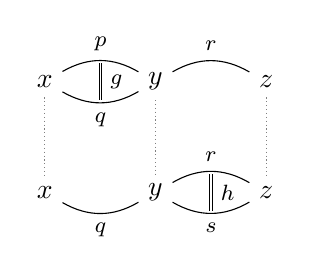
\begin{tikzpicture}[node distance=4em, baseline=(basenode.base)]
        \node[] (x1) {$x$};
        \node[right of=x1] (y1) {$y$};
        \node[right of=y1] (z1) {$z$};
        \node[below of=x1] (x2) {$x$};
        \node[right of=x2] (y2) {$y$};
        \node[right of=y2] (z2) {$z$};
        \draw[bend left] (x1) to node[above] (p) {\footnotesize$p$} (y1);
        \draw[bend right] (x1) to  node[below] (q1) {\footnotesize$q$} (y1);
        \draw[bend left] (y1) to node[above] (r1) {\footnotesize$r$} (z1);
        \draw[bend left] (y2) to node[above] (r2) {\footnotesize$r$} (z2);
        \draw[bend right] (y2) to  node[below] (s) {\footnotesize$s$} (z2);
        \draw[bend right] (x2) to node[below] (q2) {\footnotesize$q$} (y2);
        \draw[double, shorten >=.1em, shorten <=.1em] (p) to node[right] {\footnotesize$g$} (q1);
        \draw[double, shorten >=.1em, shorten <=.1em] (r2) to node[right] {\footnotesize$h$} (s);
        \draw[gray,densely dotted] (x1) to node (basenode){} (x2) (y1) to (y2) (z1) to (z2);
      \end{tikzpicture}%
      =%
      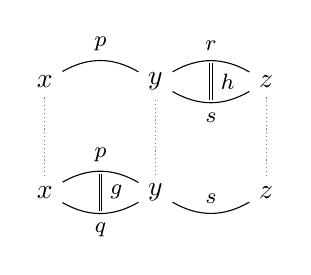
\begin{tikzpicture}[node distance=4em, baseline=(basenode.base)]
        \node[] (x1) {$x$};
        \node[right of=x1] (y1) {$y$};
        \node[right of=y1] (z1) {$z$};
        \node[below of=x1] (x2) {$x$};
        \node[right of=x2] (y2) {$y$};
        \node[right of=y2] (z2) {$z$};
        \draw[bend left] (x2) to node[above] (p) {\footnotesize$p$} (y2);
        \draw[bend right] (x2) to  node[below] (q1) {\footnotesize$q$} (y2);
        \draw[bend right] (y2) to node[above] (r1) {\footnotesize$s$} (z2);
        \draw[bend left] (y1) to node[above] (r2) {\footnotesize$r$} (z1);
        \draw[bend right] (y1) to  node[below] (s) {\footnotesize$s$} (z1);
        \draw[bend left] (x1) to node[above] (p2) {\footnotesize$p$} (y1);
        \draw[double, shorten >=.1em, shorten <=.1em] (p) to node[right] {\footnotesize$g$} (q1);
        \draw[double, shorten >=.1em, shorten <=.1em] (r2) to node[right] {\footnotesize$h$} (s);
        \draw[gray,densely dotted] (x1) to node (basenode){} (x2) (y1) to (y2) (z1) to (z2);
      \end{tikzpicture}%
    \end{sidecaption}
  \end{figure}%
  %
  One prove such a result by induction on $h$. Indeed, when
  $h\jdeq \refl r$, then both sides of the equation reduces through
  path algebra to $\ap {r\cdot\blank} (g)$. Now we are interested in
  this result when $x,y,z$ are all definitionally $a$, and $p,q,r,s$
  are all definitionally $\refl a$. In that case, one has that
  $\ap {\refl a\cdot \blank}$ and $\ap {\blank\cdot\refl a}$ both act
  trivially, and the equation becomes: $h\cdot g = g \cdot h$.

  One still has to prove that the function $\loopspace$ is an inverse
  for $\BB$. Given an abelian group $G$, the proof
  of~\cref{lemma:universal-cover-simply-connected} gives an
  equivalence between $\B\loopspace {(\BB G)}$ and the connected
  component of $\id_{\BG_\div}$ in $\BG_\div=\BG_\div$. By
  definition, this is the classifying type of $\grpcenter(G)$. Being
  abelian, $G$ is isomorphic to its center
  (\cref{def:abelian-groups}), and so it yields an element of
  $\loopspace {(\BB G)} =_{\typegroup} G$. %
  \marginnote[-1.5\baselineskip]{%
    If $X \ptdweq Y$ denote the type of pointed equivalences between
    pointed types $X,Y:\UUp$, then the univalence axiom implies that
    there is an equivalence
    \begin{displaymath}
      (X=Y) \weq (X \ptdweq Y).
    \end{displaymath}%
  }%
  Conversely, take a pointed simply connected $2$-type $(A,a)$. One
  wants to prove $\BB (\loopspace {(A,a)}) \weq_\ast (A,a)$. One
  should first notice that, because $\loopspace (A,a)$ is an abelian
  group,
  \begin{fullwidth}
  \begin{equation}
    \label{eq:loopspace-A-abelian}%
    {\B\loopspace \left( \BB (\loopspace {(A,a)}) \right)}
    \weq \conncomp{((a=a)=(a=a))}{\refl{a=a}} \weq (a=a,\refl a).
  \end{equation}
\end{fullwidth}
  This equivalence maps a path
  \begin{displaymath}
    (p,!):(a=a,\settrunc{\refl{a=a}})=(a=a,\settrunc{\refl{a=a}})
  \end{displaymath}
  to the evaluation $p(\refl a): a=a$.

  %% OLD MATERIAL, can still be useful.
  %%
  % We will now provide
  % \begin{displaymath}
  %   \Phi : \BB {(\loopspace {(A,a)})} \ptdto (A,a)
  % \end{displaymath}
  % such that $\loopspace(\Phi)$ is the previous equivalence.
  % To be able to
  % express $\Phi$, we need a small gadget about truncations of
  % function
  % types: for types $X,Y:\UU$, given an element
  % $f_0:\setTrunc{X\to Y}$, one constructs a map
  % $\lceil f_0 \rceil : \setTrunc X \to \setTrunc Y$; the type of
  % $\lceil f_0 \rceil$ being a set, one might as well suppose that
  % $f_0 \jdeq \settrunc f$ for some $f:X\to Y$; then we set
  % $\lceil f_0 \rceil (\settrunc x) = \settrunc{f(x)}$, which
  % suffices
  % in order to define $\lceil f_0 \rceil$ entirely because its
  % codomain
  % $\setTrunc Y$ is a set. If we assume the axiom of
  % choice\footnote{What is the status of AC in this book??}, then
  % $\lceil \blank \rceil$ is injective when $Y$ is a set.
  %%
  We will now define a pointed map
  $\Phi : (A,a) \ptdto \BB (\loopspace {(A,a)})$, and prove
  subsequently that this is an equivalence. Let $T : A \to \UU$ be the
  type family define by
  \begin{displaymath}
    T(a') \defequi \sum_{\alpha:\setTrunc{(a=a)\weq(a=a')}}
    \prod_{p:a=a'}\alpha=\settrunc {p\cdot\blank}
  \end{displaymath}
  We claim that $T(a')$ is contractible for all $a':A$. By
  connectedness of $A$, it is equivalent to showing that $T(a)$ is
  contractible. However
  \begin{align*}
    T(a)
    &\jdeq \sum_{\alpha:\setTrunc{(a=a)\weq(a=a)}}\prod_{p:a=a}
      \alpha = \settrunc {p\cdot \blank}
    \\
    &\weq \sum_{\alpha:\setTrunc{(a=a)\weq(a=a)}} \alpha = \settrunc{\id_{a=a}}
    \\
    &\weq 1
  \end{align*}
  Let then $\Phi (a')$ be the element
  $(a=a', \kappa_{a'}):\univcover \UU {a=a}$ where $\kappa_{a'}$ is
  the first projection of the center of contraction of $T(a')$. In
  particular, following the chain of equivalences above, $\Phi(a)$ is
  defined as $(a=a, \settrunc{\refl {a=a}})$, hence $\Phi(a)$ is
  trivially pointed by a reflexivity path. To verify that $\Phi$, thus
  defined, is an equivalence, one can use connectedness of
  $\BB(\loopspace (A,a))$ and only check that
  $\inv\Phi(a=a,\settrunc{\refl {a=a}})$ is contractible. However,
  \begin{displaymath}
    \inv\Phi(a=a,\settrunc{\refl {a=a}}) \simeq \sum_{a':A}
    \sum_{\varphi : (a=a) \weq (a=a')}\settrunc{\varphi} = \kappa_{a'}.
  \end{displaymath}
  For an element $a':A$ together with $\varphi: (a=a) \weq (a=a')$
  such that the proposition $\settrunc \varphi = \kappa_{a'}$ holds, a
  path between $(a,\id_{a=a},!)$ and $(a',\varphi,!)$ consists of a
  path $p:a=a'$ and a path $q:(x\mapsto p x) = \varphi$. We have a
  good candidate for $p$, namely $p\defequi \varphi(\refl
  a):a=a'$. However we don't have quite $q$ yet. Consider, for any
  $a':A$, the function
  \begin{displaymath}
    \ev_{\refl a}^{a'} :
    \left(
      (a=a, \settrunc{\refl{a=a}} ) =
      (a=a', \kappa_{a'} )
    \right)
    \to (a=a')
  \end{displaymath}
  defined as $(\psi,!) \mapsto \psi(\refl a)$.
  Note that $\ev_{\refl a}^{a}$ is precisely the equivalence
  $\B\loopspace{(\BB\loopspace(A,a))}_\div \weq (a=a)$ described
  in~\cref{eq:loopspace-A-abelian}. Hence, by connectedness of $A$,
  one gets that the proposition $\isEq(\ev_{\refl a}^{a'})$ holds for
  all $a':A$. In particular, because the propositions
  $\settrunc \varphi = \kappa_{a'}$ and
  $\settrunc {p\cdot\blank} = \kappa_{a'}$ holds, one gets elements
  $(\varphi,!)$ and $(x\mapsto px,!)$ in the domain of
  $\ev_{\refl a}^{a'}$. Their image $\ev_{\refl a}^{a'}(\varphi,!)$
  and $\ev_{\refl a}^{a'}(x\mapsto px,!)$ are both equal to $p$, which
  provides a path $(x\mapsto px,!)=(\varphi,!)$ in the domain. The
  first component is the path $q:(x\mapsto px) = \varphi$ that we
  wanted.
\end{proof}


\section{$G$-sets vs $\abstr(G)$-sets}
\label{sec:Gsetsabstrconcr}
\marginnote{Recall from \cref{def:abstrGtorsors} that the type of $\abstr(G)$-set is
  $$Set_{\abstr(G)}^\abstr\defequi \sum_{\mathcal X:\Set}\Hom_\abstr({\abstr(G)},\abstr(\Sigma_{\mathcal X})).$$}

Given a group $G$ it should by now come as no surprise that the type of $G$-sets is equivalent to the type of $\abstr(G)$-sets.
According to \cref{lem:homomabstrconcr}
$$\abstr:\Hom(G,\Sigma_{\mathcal X})\to\Hom^\abstr(\abstr(G),\abstr(\Sigma_{\mathcal X}))$$
is an equivalence, where the group $\Sigma_{\mathcal X}$ (as a pointed connected groupoid) is the component of the groupoid $\Set$, pointed at $\mathcal X$.  The component information is moot since we're talking about pointed maps from $\BG$ and we see that $\Hom(G,\Sigma_{\mathcal X})$ is equivalent to $\sum_{F:\BG_\div\to\Set}(\mathcal X=F(\shape_G))$.  Finally,
$$\mathrm{pr}:\sum_{\mathcal X}\sum_{F:\BG_\div\to\Set}(\mathcal X=F(\shape_G))\we
(\BG_\div\to\Set),\quad \mathrm{pr}(\mathcal X,F,p)\defequi F
$$
is an equivalence (since $\sum_{\mathcal X}(\mathcal X=F(\shape_G))$ is contractible).
Backtracking these equivalences we see that we have established
\begin{lemma}
  \label{lem:actionsconcreteandabstract}
  Let $G$ be a group.  Then the map
  $$\ev_{\shape_G}:\GSet\to\Set^\abstr_{\abstr(G)},\qquad \ev_{\shape_G}(X)\defequi(X(\shape_G),a_X)
$$
is an equivalence, where the homomorphism $a_X:\Hom^\abstr(\abstr(G), \abstr(\Sigma_{X(\shape_G)}))$ is given by transport $X:\USym G\defequi(\shape_G=\shape_G)\to (X(\shape_G)=X(\shape_G))$.
\end{lemma}
If $X$ is a $G$-set, $g:\USym G$ and $x:X(\shape_G)$, we seek forgiveness for writing $g\cdot x:X(\shape_G)$ instead of $\cast(a_X(g))(x)$.\footnote{and I ask forgiveness for strongly disliking the use of ``$\cast$'' as a name for some tacitly understood map!}

\begin{example}
  \label{ex:abstrandconj}
  Let $H$ and $G$ be groups.  Recall that the set of homomorphisms from $H$ to $G$ is a $G$-set in a natural way:
$$\Hom(H,G):\BG\to\Set,\quad \Hom(H,G)(y)\defequi \sum_{F:\BH_\div\to \BG_\div}(y=F(\shape_H)).$$

What abstract $\abstr(G)$-set does this correspond to?
In particular, under the equivalence $\abstr:\Hom(H,G)\to\Hom^\abstr(\abstr(H),\abstr(G))$, what is the corresponding action of $\abstr(G)$ on the abstract homomorphisms?

The answer is that $g:\USym G$ acts on $\Hom^\abstr(\abstr(H),\abstr(G))$ by postcomposing with conjugation $c^g$ by $g$ as defined in \cref{ex:conjhomo}.

Let us spell this out in some detail:
If $(F,p):\Hom(H,G)(\shape_G)\defequi
 \sum_{F:\BH_\div\to \BG_\div}(\shape_G=F(\shape_H))$ and $g:\USym G$, then $g\cdot(F,p)\defequi(F,p\,g^{-1})$.  If we show that the action of $g$ sends $\abstr(F,p)$ to $c^g\circ\abstr(F,p)$ we are done.

Recall that $\abstr(F,p)$ consists of the composite
$$\xymatrix{\USym H\ar[r]^-{F^=}&(F(\shape_H)=F(\shape_G))\ar[rr]^-{t\mapsto p^{-1}t\,p}&&\USym G},$$
(\ie $\abstr(F,p)$ applied to $q:\USym H $ is  $p^{-1}F^=(q)\,p$)  together with the proof that this is an abstract group homomorphism.
We see that $\abstr(F,p\,g^{-1})$ is given by conjugation:
$q\mapsto(p\,g^{-1})^{-1}F^=(q)\,(p\,g^{-1})=g\,(p^{-1}F^=(q)\,p)\,g^{-1}$, or in other words $c^g\circ\abstr(F,p)$.
\end{example}
For reference we list the conclusion of this example as a lemma:
\begin{lemma}\label{lem:abstrandconj}
  If $H$ and $G$ are groups, then the equivalence of \cref{lem:actionsconcreteandabstract} sends the $G$-set $\Hom(H,G)$ to the $\abstr(G)$-set $\Hom^\abstr(\abstr(H),\abstr(G))$ with action given by postcomposing with conjugation by elements of $\abstr(G)$.
\end{lemma}

If $f:\Hom(G,G')$ is a homomorphism, then precomposition with $\Bf:\BG\to \BG'$ defines a map $$f^*:(G'\text{-}\Set)\to(G\text{-}\Set).$$
\marginnote{Recall that \cref{lem:eq-mono-cover} told us that $f$ is an epimorphism precisely when $\USym f$ is a surjection.}
We will have the occasion to use the following result which essentially says that if $f:\Hom(G,G')$ is an epimorphism, then $f^*$ embeds the type of $G'$-sets as some of the components of the type of $G$-sets.
\begin{lemma}
  \label{lem:epifullyfaithful}
  Let $G$ and $G'$ be groups and let $f:\Hom(G,G')$ be an epimorphism.
  Then the map $f^*:(G'\text{-}\Set)\to(G\text{-}\Set)$ (induced by precomposition with $\Bf:\BG\to \BG'$) is ``fully faithful'' in the sense that if $X,Y$ are $G'$-sets, then
$$f^*:(X=Y)\to(f^*X=f^*Y)
$$
is an equivalence.
\end{lemma}
\begin{proof}
  Evaluation at $\shape_G$  yields an injective map
$$\mathrm{ev}_{\shape_G}:(f^*X=f^*Y)\to(X(f(\shape_G)=Y(f(\shape_G)))$$ and the composite
$$\mathrm{ev}_{\shape_G}f^*=\mathrm{ev}_{f(\shape_G)}:(X=Y)\to(X(f(\shape_G)=Y(f(\shape_G)))$$
 is the likewise injective, so $f^*:(X=Y)\to(f^*X=f^*Y)$ is injective.

For surjectivity, let $F':f^*X=f^*Y$ and write, for typographical convenience, $a:X(f(\shape_G)=Y(f(\shape_G))$ for $\mathrm{ev}_{\shape_G}F'\defequi F'_{\shape_G}$.
By the equivalence between $G$-sets and $\abstr(G)$-sets, $F'$ is uniquely pinned down by $a$ and the requirement that for all $g'=f(g)$ with $g:\USym G$ the diagram
$$\xymatrix{X(f(\shape_G))\ar@{=}[r]^{X({g'})}\ar@{=}[d]_{a}&
  X(f(\shape_G))\ar@{=}[d]_{a}\\
  Y(f(\shape_G))\ar@{=}[r]^{Y({g'})}&Y(f(\shape_G))}
$$
commutes.  Likewise, (using transport along the identity $p_f:\shape_{G'}=f(\shape_G)$) an $F:X=Y$ in the preimage of $a$ is pinned down by the commutativity of the same diagram, but with $g':f(\shape_G)=f(\shape_G)$ arbitrary (an a priori more severe requirement, again reflecting injectivity).   However, when $f:\USym G\to\USym {G'}$ is surjective these requirements coincide, showing that $f^*$ is an equivalence.


% Fix for the moment an  $a:X(f(\shape_G)=Y(f(\shape_G))$

% Now, by transport along the identity $p_f:\shape_{G'}=f(\shape_G)$ and the equivalence between $G'$-sets and $\abstr(G')$-sets, an identity $F':X=Y$ of $G'$-sets is uniquely pinned down by an identity $F'_{f(\shape_G)}:X(f(\shape_G)=Y(f(\shape_G))$ together with the proposition that for all $g':f(\shape_G)=f(\shape_G)$ the diagram $$\xymatrix{X(f(\shape_G))\ar@{=}[r]^{X_{g'}}\ar@{=}[d]_{F'_{f(\shape_G)}}&
%   X(f(\shape_G))\ar@{=}[d]_{F'_{f(\shape_G)}}\\
%   Y(f(\shape_G))\ar@{=}[r]^{Y_{g'}}&Y(f(\shape_G))}
% $$
% commutes.  Likewise, an identity $F:f^*X=f^*Y$ is given by exactly the same data, except that the diagram is only required to commute for $g'=f(g)$ for all $g:\USym G$.  But when $f:\USym G\to\USym {G'}$ these requirements coincide.


% ; $F:X=Y$ is in the preimage of $a:X(f(\shape_G)=Y(f(\shape_G))$ if and only if $a=F_{f(\shape_G)}$ and for all $g':f(\shape_G)=f(\shape_G)$ the diagram
% $$\xymatrix{X(f(\shape_G))\ar@{=}[r]^{X_{g'}}\ar@{=}[d]_{F_{f(\shape_G)}}&
%   X(f(\shape_G))\ar@{=}[d]_{F_{f(\shape_G)}}\\
%   Y(f(\shape_G))\ar@{=}[r]^{Y_{g'}}&Y(f(\shape_G))}
% $$
% commutes.  However, since $f$ is surjective there is a $g:\USym G$ so that $g'=f(g)$.  Therefore, anything in $f^*X=f^*Y$ which is in the preimage of $a$ is in the image of $f^*:X=Y$ and we have shown that $f^*$ is also a surjection.
\end{proof}

\section{Semidirect products}
\label{sec:Semidirect-products}{\color{red} just moved without prooreading BID 211116}

In this section we describe a generalization of the product of two group, called the {\em semidirect} product, which can be constructed from an
action of a group on a group.  Like the product, it consists of pairs, both at the level of concrete groups and of abstract groups, as we shall
see.

We start with some preliminaries on paths between pairs.
Lemma \cref{lem:isEq-pair=} above takes a simpler form when $y$ and $y'$ are values of a family $x \mapsto f(x)$
of elements of the family $x \mapsto Y(x)$, as the following lemma shows.

\begin{lemma}\label{lem:pathpairsection}
  Suppose we are given a type $X$ and a family of types $Y(x)$ parametrized by the elements $x$ of $X$.
  Suppose we are also given a function $f : \prod_{x:X} Y(x)$.
  For any elements $x$ and $x'$ of $X$,
  there is an equivalence of type
  $$\left ( (x,f(x)) = (x',f(x')) \right ) \weq (x=x') \times (f(x) = f(x)),$$
  where the identity type on the left side is between elements of $\sum_{x:X} Y(x)$.
\end{lemma}

\begin{proof}
  By \cref{lem:isEq-pair=} and by composition of equivalences, it suffices to establish an equivalence of type
  $$\left( \sum_{p:x=x'} \pathover {f(x)} Y p {f(x')} \right) \weq (x=x') \times (f(x) = f(x)).$$
  Rewriting the right hand side as a sum over a constant family, it suffices to find an equivalence of type
  $$\left( \sum_{p:x=x'} \pathover {f(x)} Y p {f(x')} \right) \weq \sum_{p:x=x'} (f(x) = f(x)).$$
  By \cref{lem:fiberwise} it suffices to establish an equivalence of type
  $$ \left( \pathover {f(x)} Y p {f(x')} \right) \weq (f(x) = f(x))$$
  for each $p:x=x'$.  By induction on $x'$ and $p$ we reduce to the case where $x'$ is $x$ and $p$ is $\refl x$, and it suffices to establish an
  equivalence of type
  $$ \left( \pathover {f(x)} Y {\refl x} {f(x)} \right) \weq (f(x) = f(x)).$$
  Now the two sides are equal by definition, so the identity equivalence provides what we need.
\end{proof}

The lemma above shows how to rewrite certain paths between pairs as pairs of paths.  Now we wish to establish the formula for composition of
paths, rewritten in terms of pairs of paths, but first we introduce a convenient definition for the transport of loops in $Y(x)$ along paths in
$X$.

\begin{definition}\label{def:pathsectionaction}
  Suppose we are given a type $X$ and a family of types $Y(x)$ parametrized by the elements $x$ of $X$.
  Suppose we are also given a function $f : \prod_{x:X} Y(x)$.
  For any elements $x$ and $x'$ of $X$ and for any identity $p : x = x'$, define a function $(f(x') = f(x')) \to (f(x) = f(x))$, to be denoted
  by $q' \mapsto {q'} ^ p$, by induction on $p$ and $x'$, reducing to the case where $x'$ is $x$ and $p$ is $\refl x$, allowing us to
  set ${q'} ^{ \refl x } \defeq q'$.
\end{definition}

We turn now to associativity for the operation just defined.

\begin{lemma}\label{def:pathsectionactionassoc}
  Suppose we are given a type $X$ and a family of types $Y(x)$ parametrized by the elements $x$ of $X$.
  Suppose we are also given a function $f : \prod_{x:X} Y(x)$.
  For any elements $x$, $x'$, and $x''$ of $X$, for any identities $p : x = x'$ and $p' : x' = x''$,
  and for any $q : f x'' = f x''$,
  there is an identification of type $ ( q ^{ p' }) ^ p = q ^{( p' \cdot p )}$.
\end{lemma}

\begin{proof}
  By induction on $p$ and $p'$, it suffices to show that $ ( q ^{ \refl y }) ^ { \refl y } = q ^{( \refl y \cdot \refl y )}$, in which both sides are
  equal to $q$ by definition.
\end{proof}

Observe that the operation depends on $f$, but $f$ is not included as part of the notation.

The next lemma contains the formula we are seeking.

\begin{lemma}\label{lem:pathpairsectionmult}
  Suppose we are given a type $X$ and a family of types $Y(x)$ parametrized by the elements $x$ of $X$.
  Suppose we are also given a function $f : \prod_{x:X} Y(x)$.
  For any elements $x$, $x'$, and $x''$ of $X$, and for any two identities $e : (x,f(x)) = (x',f(x'))$ and $e' : (x',f(x')) = (x'',f(x''))$,
  if $e$ corresponds to the pair $(p,q)$ with $p : x = x'$ and $q : f x = f x$ under the equivalence of \cref{lem:pathpairsection},
  and $e'$ corresponds to the pair $(p',q')$ with $p' : x' = x''$ and $q' : f x' = f x'$,
  then $e' \cdot e$ corresponds to the pair $(p' \cdot p , ({q'} ^ p) \cdot q)$.
\end{lemma}

\begin{proof}
  By induction on $p$ and $p'$ we reduce to the case where $x'$ and $x''$ are $x$ and $p$ and $p'$ are $\refl x$.
  It now suffices to show that $e' \cdot e$ corresponds to the pair $(\refl x , q' \cdot q)$.
  Applying the definition of the map $\Phi$ in the proof of \cref{lem:isEq-pair=} to our three pairs, we see that it suffices to show that
  $\left( \apap g {\refl x} {q'} \right) \cdot \left( \apap g {\refl x} {q} \right) = \apap g {\refl x} {q' \cdot q}$, with $g$, as there, being the function $ g(x)(y) \defeq (x,y)$.
  By \cref{def:applfun2comp} it suffices to show that $\left( \ap {g(x)} {q'} \right) \cdot \left( \ap {g(x)} {q} \right) = \ap {g(x)} {(q' \cdot q)}$, which follows from
  compatibility of $\ap {g(x)}$ with composition, as in \cref{lem:apcomp}.
\end{proof}

The lemma above will be applied mostly in the case where $x'$ and $x''$ are $x$, but if it had been stated only for that case, we would not have
been able to argue by induction on $p$ and $p'$.

\begin{definition}\label{def:semidirect-product}
  Given a group $G$ and an action $\tilde H : \BG \to \typegroup$ on a group $H \defeq \tilde H(\shape_G)$, we define a group called the {\em
    semidirect product} as follows.
  $$G \ltimes \tilde H \defeq \mkgroup { \sum_{t:\BG} \B \tilde H(t) }$$
  Here the basepoint of the sum is taken to be the point $(\shape_G,\shape_H)$.
  (We deduce from \cref{lem:level-n-utils}, \cref{level-n-utils-sum}, that $\sum_{t:\BG} \B \tilde H(t)$ is a groupoid.
  See \cref{lem:UNKNOWN} for a proof that $\sum_{t:\BG} \B \tilde H(t)$ is connected.)
\end{definition}

Observe that if the action of $G$ on $H$ is trivial, then $\tilde H(t) \jdeq H$ for all $t$ and $G \ltimes \tilde H \jdeq G \times H$.

Projection onto the first factor gives a homomorphism $p \defeq \mkgroup \fst : G \ltimes \tilde H \to G$.
Moreover, there is a homomorphism $s : G \to G \ltimes \tilde H$ defined by
$ s \defeq \mkgroup {\left( t \mapsto (t,\shape_{\tilde H(t)}) \right) }$, for $t : \B G$.
The two maps are homomorphisms because they are made from basepoint-preserving maps.
The map $s$ is a \emph{section} of $p$ in the sense the $p \circ s = \id_G$.
There is also a homomorphism $j : H \to G \ltimes \tilde H$ defined by $j \defeq \mkgroup { \left( u \mapsto (\shape_G,u) \right) }$, for $u : \B H$.

\begin{lemma}
  The homomorphism $j$ above is a monomorphism, and it gives the same (normal) subgroup of $G \ltimes \tilde H$ as the kernel $\ker p$ of $p$.
\end{lemma}
\footnote{{\color{red}MUST BE MOVED TO THE SUBGROUP CHAPTER}}

\begin{proof}
  See \ref{def:kernel} for the definition of kernel.  According to \cref{lem:fst-fiber(a)=B(a)}, the map $\B H \to (\B p)^{-1}(\shape_G)$ defined by
  $ u \mapsto ((\shape_G,u), \refl{\shape_G}) $ is an equivalence.  This establishes that the fiber $(\B p)^{-1}(\shape_G)$ is connected and thus serves as
  the classifying type of $\ker p$.  Pointing out that the composite map $H \xrightarrow{\isom} \ker p \to G \ltimes \tilde H$ is $j$ and using
  univalence to promote the equivalence to an identity gives the result.
\end{proof}

Our next goal is to present the explicit formula for the multiplication operation in $\USym { G \ltimes \tilde H }$.
First we apply \cref{lem:pathpairsection} to get a bijection $\USym { G \ltimes \tilde H } \weq \USym G \times \USym H$.
Now use that to transport the multiplication operation of the group $\USym { G \ltimes \tilde H }$ to the set $\USym G \times \USym H$.
Now \cref{lem:pathpairsectionmult} tells us the formula for that transported operation is given as follows.
$$ (p',q') \cdot (p,q) = (p' \cdot p , ({q'} ^ p) \cdot q) $$
In a traditional algebra course dealing with abstract groups, this formula is used as the definition of the multiplication operation
on the set $\USym G \times \USym H$, but then one must prove that the operation satisfies the properties of \cref{def:abstractgroup}.
The advantage of our approach is that the formula emerges from the underlying logic that governs how composition of paths works.


\section{The pullback}
\label{sec:pullback}
Given two functions $f:B\to D$ and $g:C\to D$ with common target, the ``pullback'' which we will now define should be thought about as the type of all pairs of elements $(b,c):B\times C$ so that $f(b)=g(c)$.  This construction is important in many situations also beyond group theory.

\begin{definition}
  \label{def:pullback}
  Let $B, C, D$ be types and let $f:B\to D$ and $g:C\to D$ be two maps.
The \emph{pullback}\index{pullback} of $f$ and $g$ is the type
$$\prod(f,g)\defequi\sum_{(b,c):B\times C}(f(b)=_Dg(c))$$
together with the two projections $\prj_B:\prod(f,g)\to B$ and $\prj_C:\prod(f,g)\to C$ sending $(b,c,p):\prod(f,g)$ to $b:B$ or $c:C$.  If $f$ and $g$ are clear from the context, we may write $B\times_DC$ instead of $\prod(f,g)$ and summarize the situation by the diagram
$$\xymatrix{B\times_DC\ar[r]^{\prj_C}\ar[d]^{\prj_B}&C\ar[d]^g\\B\ar[r]^f&\,D.}$$
\end{definition}
\begin{xca}
  \marginnote{Illustrating the exercise: if the solid diagram commutes there is a unique dotted arrow so that the resulting diagram commutes:
    $$\xymatrix{A\ar@{.>}[dr]\ar[drr]\ar[ddr]&&\\
    &B\times_DC\ar[r]\ar[d]&C\ar[d]\\&B\ar[r]&D}
  $$}
  \label{xca:univpropofpullback}
  Let $f:B\to D$ and $g:C\to D$ be two maps with common target.  If $A$ is a type show that
  \begin{align*}
    (A\to B)\times_{(A\to D)}(A\to C)\to &(A\to B\times_DC)\\
(\beta,\gamma,p:f\beta=g\gamma)\,\mapsto\,&(a\mapsto (f(a),g(a),p(a):f\beta(a)=g\gamma(a)))
  \end{align*}
 is an equivalence.
\end{xca}
In view of \cref{xca:univpropofpullback} we will say that we have a \emph{pullback diagram}\index{pullback diagram}
$$\xymatrix{A\ar[d]^{g'}\ar[r]^{f'}&C\ar[d]^g\\B\ar[r]^f&D}$$
to indicate that we have an element in $(A\to B)\times_{(A\to D)}(A\to C)$ such that the resulting map $A\to B\times_DC$ is an equivalence.

\begin{example}
  \marginnote{Preimage as a pullback: $$\xymatrix{f^{-1}(d)\ar[d]\ar[r]&\bn1\ar[d]^d\\B\ar[r]^f&D}$$}
  If $g:\bn 1\to D$ has value $d:D$ and $f:B\to D$ is any map, then $\prod(f,g)\oldequiv B\times_D\bn 1$ is equivalent to the preimage $f^{-1}(d)\defequi\sum_{b:B}d=f(b)$.
\end{example}
\begin{example}
  \label{ex:pullbackandgcd}
  Much group theory is hidden in the pullback.  For instance, the greatest common divisor $\gcd(a,b)$ of $a,b:\NN$ is another name for the number of components you get if you pull back the $a$-fold and the $b$-fold \coverings of the circle: we % will see in \cref{lem:iso2} we
  have a pullback
$$\xymatrix{S^1\times\B C_{\gcd(a,b)}\ar[d]\ar[r]& S^1\ar[d]^{(-)^b}\\
S^1\ar[r]^{(-)^a}&\,S^1}
$$
(where $C_n$ was the cyclic group of order $n$).
To get a geometric idea, think of the circle as the unit circle in the complex numbers so that the $a$-fold \covering is simply taking the $a$-fold power.  With this setup, the pullback should consist of pairs $(z_1,z_2)$ of unit length complex numbers with the property that $z_1^a=z_2^b$.  Let $a=a'\gcd(a,b)$ and $b=b'\gcd(a,b)$. Taking an arbitrary unit length complex number $z$, then the pair $(z^{b'},z^{a'})$ is in the pull back (since $a'b=ab'$).  But so is $(\zeta z^{b'},z^{a'})$, where $\zeta$ is any $\gcd(a,b)$\th root of unity.  Each of the $\gcd(a,b)$-choices of $\zeta$ contributes in this way to a component of the pullback.  In more detail: identifying the cyclic group $C_{\gcd(a,b)}$ of order $\gcd(a,b)$ with the group of $g$\th roots of unity, the top horizontal map $S^1\times C_{\gcd(a,b)}\to S^1$ sends $(z,\zeta)$ to $z^{a'}$ and the left vertical map sends $(z,\zeta)$ to the product $\zeta z^{b'}$.

Also the least common multiple $\lcm(a,b)=a'b$ is hidden in the pullback; in the present example it is demonstrated that the map(s) accross the diagram makes each component of the pullback a copy of the $\lcm(a,b)$-fold \covering.
\end{example}


\begin{definition}
  \label{def:intersectionand unionofsets}
  Let $S$ be a set and consider two subsets $A$ and $B$ of $S$ given by two families of propositions (for $s:S$) $P(s)$ and $Q(s)$.  The \emph{intersection}\index{intersection! of sets} $A\cap B$ of the two subsets is given by the family of propositions $P(s)\times Q(s)$.  The \emph{union}\index{union of sets} $A\cup B$ is given by the set family of propositions $A(s)+B(s)$.
\end{definition}
\begin{xca}
  \label{xca:intersectionpullbackofsets}
  Given two subsets $A$, $B$ of a set $S$, prove that
  \begin{enumerate}
  \item The pullback $A\times_SB$ maps by an equivalence to the intersection $A\cap B$,
  \item\label{xca:cardinalityintersectionunion}
    If $S$ is finite, then the sum of the cardinalities of $A$ and $B$ is equal to the sum of the cardinalities of $A\cup B$ and $A\cap B$.\qedhere
  \end{enumerate}
\end{xca} 

\begin{definition}
  \label{def:intersectionofgroups}
  Let $f:\Hom(H,G)$ and $f':\Hom(H',G)$ be two homomorphisms with common target.  The \emph{pullback}\index{pullback!of groups} $H\times_GH'$ is the group obtained as the (pointed) component of
$$\pt_{H\times_GH'}\defequi(\shape_H,\pt_{H'},p_{f'}p_f^{-1})$$ of the pullback $\BH\times_{\BG}\BH'$ (where $p_f:\shape_G=f(\shape_H)$ is the name we chose for the data displaying $f$ as a pointed map, so that $p_{f'}p_f^{-1}:f(\shape_H)=f'(\pt_{H'})$).

If $(H,f,!)$ and $(H',f',!)$ are monomorphisms into $G$, then the pullback is called the \emph{intersection}\index{intersection! of monomorphisms} and if the context is clear denoted simply $H\cap H'$.
\end{definition}
\begin{example}
  If $a,b:\NN$ are natural number with least common multiple $L$, then $L\ZZ$ is the intesection $a\ZZ\cap b\ZZ$ of the subgroups $a\ZZ$ and $b\ZZ$ of $\ZZ$.
\end{example}
% \begin{example}this came out wrong DELETE June
%   If $H,K:\typemono_G$ with $X,Y:\BG\to\Set$ being the corresponding transitive $G$-sets under the equivalence $E$, then the intersection of $H$ and $K$ corresponds to the $G$-set $X\times Y:\BG\to\Set$ (with $(X\times Y)(x)\defequi X(x)\times Y(x)$).
% \end{example}

\begin{xca}
  Prove that if $f:\Hom(H,G)$ and $f':\Hom(H',G)$ are homomorphisms,
  then the pointed version of \cref{xca:univpropofpullback} induces an equivalence
  \[
    \USymH \times_{\USymG} \USymH'
    \simeq (\shape_{H\times_GH'}=\shape_{H\times_GH'}).\text{\footnotemark}
  \]
  Elevate this equivalence to a statement about abstract groups.\footnotetext{%
    Hint: set $A\defequi \Sc$, $B\defequi \BH$, $C\defequi \BH'$ and $D\defequi \BG$.}
\end{xca}



\section{Sums of groups}
\label{sec:coprod}
We have seen how the group of integers $\ZZ=(S^1,\base)$ synthesizes the notion of one symmetry with no relations: every symmetry in the circle is of the form $\Sloop^n$ for some unique $n$.  Also, given any group $G=\aut_A(a)$, the set $a=a$ of symmetries of $a$ corresponds to the set of homomorphisms $\ZZ\to G$, \ie to pointed functions $(S^1,\base)\to_*(A,a)$ by evaluation at $\Sloop$.  What happens if we want to study more than one symmetry at the time?

For instance, is there a group $\ZZ\vee\ZZ$ so that for any group $G=\aut_A(a)$ a homomorphism $\ZZ\vee\ZZ\to G$ corresponds to \emph{two} symmetries of $a$?
At the very least, $\ZZ\vee\ZZ$ itself would have to have two symmetries and these two can't have any relation, since in a general group $G=\aut_A(a)$ there is a priori no telling what the relation between the symmetries of $a$ might be.
Now, \emph{one} symmetry is given by a pointed function $(S^1,\base)\to_*(A,a)$ and so a \emph{pair} of symmetries is given by a function $f:S^1+S^1\to A$ with the property that $f$ sends each of the base points of the circles to $a$.  But $S^1+S^1$ is not connected, and so not a group.  To fix this we take the clue from the requirement that both the base points were to be sent to a common base point and \emph{define} $S^1\vee S^1$ to be what we get from $S^1+S^1$ when we \emph{insert an identity} between the two basepoints.
\marginnote{$S^1\vee S^1$ if formed from $S^1+S^1$ by inserting an identity$$\xymatrix{\base\ar@(ul,dl)[]|{\Sloop}\ar@{.>}[rr]^{\text{identify!}}&&\base\ar@(ur,dr)[]|{\Sloop}}
  $$}

The amazing thing is that this works -- an enormous simplification of the classical construction of the ``free products'' or ``amalgamated sum'' of groups.  We need to show that the ``wedge'' $S^1\vee S^1$ is indeed a group, and this proof simultaneously unpacks the classical description.

We start by giving a definition of the wedge construction which is important for pointed types in general and then prove that the wedge of two groups is a group whose symmetries are arbitrary ``words'' in the original symmetries.

\begin{definition}
  \label{def:wedge}
  Let $(A_1,a_1)$ and $(A_2,a_2)$ be pointed types.  The \emph{wedge}\index{wedge of pointed types} is the pointed type $(A_1\vee A_2,a_{12})$ given as a higher inductive type by
  \begin{enumerate}
  \item functions $i_1:A_1\to A_1\vee A_2$ and $i_2:A_2\to A_1\vee A_2$
  \item an identity $g:i_1a_1=i_2a_2$.
  \end{enumerate}
We point this type at $a_{12}\defequi i_1a_1$.
  The function
$$i^g_2:(a_2=_{A_2}a_2)\to(a_{12}=_{A_1\vee A_2}a_{12})$$
is defined by $i^g_2(p)\defequi g^{-1}i_2(p)g$, whereas (for notational consistency only) we set $i_1^g\defequi i_1:(a_1=_{A_1}a_1)\to(a_{12}=_{A_1\vee A_2}a_{12})$.
Simplifying by writing $i:A_1+A_2\to A_1\vee A_2$ for the function given by $i_1$ and $i_2$ (with basepoints systematically left out of the notation),
the induction principle is
$$\prod_{C:(A_1\vee A_2)\to\UU}\sum_{s:\prod_{a:A_1+A_2}Ci(a)}
((s(a_1)=C(g^{-1})s(a_2))\,\to\,\prod_{x:(A_1\vee A_2)}C(x)).$$
\end{definition}

Unraveling the induction principle we see that if $B$ is a pointed type, then a  pointed function $f:A_1\vee A_2\to_* B$ is given by providing pointed functions $f_1:A_1\to_* B$ and $f_2:A_2\to_* B$  -- the identity $f_1(a_1)=f_2(a_2)$ which seems to be missing is provided by the requirement of the functions being pointed.  For the record
\begin{lemma}
  \label{lem:univvee}
  If $B$ is a pointed type, then the function
  $$i^*:(A_1\vee A_2\to_*B)\to(A_1\to_*B)\times(A_2\to_*B),\qquad i^*(f)=(fi_1,fi_2)
$$
is an equivalence.
\end{lemma}



To the right you see a picture of $i_2^g(p)$: \marginnote{$$
\xy (-20,20)*+{};(-20,20)*+{}
**\crv{(15,20)&(18,20)&(-10,35)&(10,45)&(25,30)&(20,19)&(0,20)}
%?>*\dir{>}
?(0)*{} *!LD!/^-20pt/{i_1A_1}
?(.45)*{} *!LD!/^2pt/{>}
?(.95)*{} *!LD!/^-15pt/{g^{-1}}
?(.03)*{} *!LD!/^-5pt/{g}
?(.55)*{} *!LD!/^-7pt/{i_2p}
?(.65)*{} *!LD!/^-30pt/{i_2A_2}
?(.87)*{} *!LD!/^-12pt/{i_2a_2}
?(.86)*{} *!LD!/^-2pt/{\bullet}
?(1)*{} *!LD!/^-2pt/{\bullet}
?(1)*{} *!LD!/^-12pt/{a_{12}}
\endxy
$$}it is the symmetry of the base point $a_{12}\defequi i_1a_1$ you get by \emph{first} moving to $i_2a_2$ with $g$, \emph{then} travel around with $p$ ($i_2p$, really) and finally go home to the basepoint with the inverse of $g$.

\marginnote{The idea is that an identity in $a_{12}=x$ can be factored into a string of identities, each lying solely in $A_1$ or in $A_2$.  We define a family of sets consisting of exactly such strings of identities --  it is a set since $A_1$ and $A_2$ are groupoids -- and prove that it is equivalent to the family $P(x)\defequi(a_{12}=_{A_1\vee A_2}x)$ which consequently must be a family of sets.
We need to be able to determine whether a symmetry is reflexivity or not, but once we know that, the symmetries of the base point in the wedge are then given by ``words $p_0p_1\dots p_n$'' where the $p_j$ alternate between being symmetries in the first or the second group, and none of the $p_j$ for positive $j$ are allowed to be reflexivity.  Note that there order of the $p_j$s is not negotiable: if I shuffle them I get a new symmetry.}


\begin{definition}
  \label{def:sumofgroup}
  If $G_1=\aut_{A_1}(a_1)$ and $G_2=\aut_{A_2}(a_2)$ are groups, then their \emph{sum}\index{sum of groups} is defined as
  $$G_1\vee G_2\defequi \aut_{A_1\vee A_2}(a_{12}).$$
  The homomorphisms $i_1:G_1\to G_1\vee G_2$ and $i_2:G_2\to G_1\vee G_2$ induced from the structure maps  $i_1:A_1\to A_1\vee A_2$ and  $i_2:A_2\to A_1\vee A_2$ are also referred to as \emph{structure maps}.
\end{definition}
\begin{lemma}
  \label{lem:sumofgroupsISsum} If $G_1$, $G_2$ and $G$ are groups, then the function
  $$\Hom(G_1\vee G_2,G)\to\Hom(G_1,G)\times\Hom(G_2,G)$$
given by restriction along the structure maps is an equivalence.
\end{lemma}
\begin{proof}
  This is a special case of \cref{lem:univvee}.
\end{proof}
Specializing further, we return to our initial motivation and see that mapping out of a wedge of two circles \emph{exactly} captures the information of two independent symmetries:
\begin{corollary}
  \label{cor:ZplusZuniv}
  If $G$ is a group, then the functions
  $$\Hom(\ZZ\vee\ZZ,G)\to \Hom(\ZZ,G)\times\Hom(\ZZ,G)\simeq \USym G\times \USym G$$
  is an equivalence.
\end{corollary}
\begin{xca}
This leads to the following characterization of abelian groups formulated purely in terms of pointed connected groupoids (no reference to the identity types).
  \label{xca:whatAREabeliangroups}
  A group $G$ is abelian if and only if the canonical map

  \marginnote{$$\xymatrix{G\vee G\ar[r]^+\ar[d]_{\text{inclusion}}&G\\
      G\times G\ar@{.>}[ur]}$$}
$$+:G\vee G\to G$$
(given via \cref{lem:sumofgroupsISsum} by $\id_G:G\to G$) extends over the inclusion
$$i:G\vee G\to G\times G$$
(given by the inclusions $\mathrm{in}_1,\mathrm{in}_2:G\to G\times G$).\footnote{I haven't written out a formalization myself}

As a cute aside, one can see that the required map $\BG\times\BG\to_*\BG$ actually doesn't need to be pointed:
factoring $+:\BG\vee\BG\to_*\BG$ over $i:\BG\vee\BG\to_*\BG\times\BG$
-- even in an unpointed way -- kills all ``commutators''
$ghg^{-1}h^{-1}:\USym(G\vee G)$.
\end{xca}

We end the section by proving that wedges of decidable groups are decidable groups and that they can be given the classical description in terms of words.


\begin{lemma}
  \label{lem:wedgeofgpoidisgpoid}
  Let $G_1\defequi\aut_{A_1}(a_1)$ and $G_2\defequi\aut_{A_2}(a_2)$ be decidable groups, then the wedge sum $G_1\vee G_2\defequi\aut_{A_1\vee A_2}(a_{12})$ is a decidable group.

Let $C_1$ be the set of strings $(p_0,n,p_1,\dots,p_n)$ with $n:\NN$ and, for $0\leq j\leq n$
\begin{itemize}
\item $p_{j}:\USym G_1%\defequi (a_1=a_1)
  $  for even $j$
\item $p_{j}:\USym G_2%\defequi (a_2=a_2)
  $ for odd $j$ and
\item $p_j$ is not reflexivity for $j$ positive
\end{itemize}
(the last requirement makes sense and is a proposition since our groups are decidable).

  Then the function given by composition in $\USym G_{12}\defequi(a_{12}=a_{12})$
  $$\beta:C_1\to\USym G_{12}%\defequi(a_{12}=a_{12})
  ,\qquad\beta(p_0,n,p_1,\dots p_n)\defequi i_1^gp_0i_2^gp_1i_1^gp_2\dots i_?^gp_n$$
(where $i_?^gp_n$  is $i_1^gp_n$ or $i_2^gp_n$ according to whether $n$ is even or odd) is an equivalence.
\end{lemma}
\begin{proof}
  That the wedge is connected follows by transitivity of identifications,
  if necessary passing through the identification $g:i_1a_1=i_2a_2$ in the wedge.

We must prove that the wedge is a groupoid, \ie that all identity types are sets, which we do by giving an explicit description of the universal \covering.

 We use the notation of \cref{def:wedge} freely, and for ease of notation, let $a_{2k+i}\defequi a_i$ and $i_{2k+i}^g\defequi i_i^g$ for $i=1,2$, $k:\NN$.
Define families of sets
$$C_i:A_i\to\Set,\qquad i=1,2$$
by
$$
C_i(x)\defequi(a_i=_{A_i}x)\times
\sum_{n:\NN}\prod_{1\leq k\leq n}\sum_{p_k:a_{i+k}= a_{i+k}}(p_k\neq\refl {a_{i+k}})
$$
when $x:A_i$.  Note that $p_k\neq\refl{a_{i+k}}$  is a proposition; we leave it out when naming elements. Hence, an element in $C_1(a)$ is a tuple
$(p_0,n,p_1,\dots,p_n)$ where $p_0:a_1=_{A_1}a$, $p_1:a_2=_{A_2}a_2$, $p_2:a_1=_{A_1}a_1$, and so on -- alternating between symmetries of $a_1$ and $a_2$, and where $p_0$ is the only identity allowed to be $\refl{}$. Define $C_{12}:C_1(a_1)\to C_2(a_2)$ by
$$C_{12}(p_0,n,p_1\dots,p_n)=
\begin{cases}
  (\refl{a_2}0,)&\text{ if }p_0=\refl{a_1}, n=0,\\
  (p_1,n-1,p_2\dots,p_n)& \text{ if }p_0=\refl{a_1},n\neq0,\\
  (\refl{a_2},n+1,p_0,\dots,p_n)& \text{ if }p_0\neq\refl{a_1}.
\end{cases}
$$
It is perhaps instructive to see a table of the values $C_{12}(p_0,n,p_1,\dots,p_n)$ for $n<3$:
\begin{center}
  \begin{tabular}{r|c cc}
    &$(p_0,0)$&$(p_0,1,p_1)$&$(p_0,2,p_1,p_2)$\\
    \hline
    $p_0=\refl{a_1}$&$(\refl{a_2},0)$&$(p_1,0)$&$(p_1,1,p_2)$\\
    $p_0\neq\refl{a_1}$&$(\refl{a_2},1,p_0)$&$(\refl{a_2},2,p_0,p_1)$&$(\refl{a_2},3,p_0,p_1,p_2)$
  \end{tabular}
\end{center}
Since $C_{12}$ is an equivalence, the triple $(C_1,C_2,C_{12})$ defines a family
$$C:A_1\vee A_2\to\Set.$$
In particular, $C(a_{12})\defequi C_1(a_1)$.
For $x:A_1$ we let $i^C_1:C_1(x)\to C(i_1(x))$ be the induced equivalence, and likewise for $i^C_2$.
We will show that $C$ is equivalent to $P\defequi \pathsp{a_{12}}$, where $P(x)\defequi(a_{12}=x)$, and so that the identity types in the wedge are equal to the sets provided by $C$.

One direction is by transport in $C$; more precisely,
$$\alpha:\prod_{x:A_1\vee A_2}(P(x)\to C(x))$$ is given by transport with $\alpha(a_{12})(\refl{a_{12}})\defequi(\refl{a_{1}},0):C(a_{12})$.
The other way,
$$\beta:\prod_{x:A_1\vee A_2}(C(x)\to P(x))$$ is given by composing identities, using the glue $g$ to make their ends meet:
$$\beta(i_1a)(p_0,n,p_1,\dots,p_n)\defequi i_1(p_0)i_2^g(p_1)i_3^g(p_2) \dots i_{n+1}^g(p_n)$$
(here the definition $\dots i_3^g\defequi i_1^g\defequi i_1$ proves handy since we don't need to distinguish the odd and even cases)
and likewise
$$\beta(i_2a)(p_0,n,p_1,\dots,p_n)\defequi i_2(p_0)g\,i_1^g(p_1)i_2^g(p_2) \dots i_{n}^g(p_n)$$ and compatibility with the glue $C_{12}$ is clear since the composite $\refl{x}p$ is equal to $p$.

For notational convenience, we hide the $x$ in $\alpha(x)(p)$ and $\beta(x)(p)$ from now on.

That $\beta\alpha(p)=p$ follows by path induction: it is enough to prove it for $x=a_{12}$ and
$p\defequi\refl{a_{12}}$:
$$\beta\alpha(\refl{a_{12}})=\beta(\refl{a_1},0)=i_1^g\refl{a_1}=\refl{a_{12}}.$$

That $\alpha\beta(p_0,n,p_1\dots,p_n)=(p_0,n,p_1,\dots,p_n)$ follows by induction on $n$ and $p_0$.  For $n=0$ it is enough to consider  $x=a_{12}$ and $p_0=\refl{a_1}$, and then
$\alpha\beta(\refl{a_1},0)\defequi\alpha(\refl{a_{12}})\defequi(\refl{a_1},0)$.  In general, (for $n>0$)
\begin{align*}
  \alpha\beta(p_0,n,p_1\dots,p_n)
=&\trp[C]{i_1(p_0)i_2^g(p_1)i_1^g(p_2) \dots i_{n+1}^g(p_n)}(\refl{a_1,0})\\
=&\trp[C]{i_1(p_0)}\dots\trp[C]{i_{n+1}^g(p_n)}(\refl{a_1,0}).
\end{align*}
  The induction step is as follows: let $0< k\leq n$, then
\begin{align*}
  &\trp[C]{i_k^gp_{k-1}}i^C_{k-1}(p_k,n-k-1,p_{k+1},\dots,p_n)\\
  =&\trp[C]{i_k^gp_{k-1}}i^C_k(\refl{a_{k-1}},n-k,p_k,\dots,p_n)\\
  =&i^C_k\trp[C_k]{p_{k-1}}(\refl{a_{k-1}},n-k,p_k,\dots,p_n)\\
  =&(p_{k-1},n-k,p_k,\dots,p_n).
\end{align*}
%((please see whether this makes sense to anybody but yvt))
\end{proof}

\section{Heaps \texorpdfstring{$(\dagger)$}{(\textdagger) \color{red} just moved from symmetry without proofreding BID211116}}
\label{sec:heaps}

Recall that we in \cref{rem:heap-preview} wondered about
the status of general identity types $a=_A a'$,
for $a$ and $a'$ elements of a groupoid $A$,
as opposed to the more special loop types $a=_Aa$.\marginnote{%
  This section has no implications for the rest of the book,
  and can thus safely be skipped on a first reading.
  (TODO: Move in place in \cref{ch:groups}?)}
Here we describe the resulting algebraic structure
and how it relates to groups.

We proceed in a fashion entirely analogous to that of \cref{sec:typegroup},
but instead of looking a pointed types, we look at \emph{bipointed types}.

\begin{definition}\label{def:bipt-conn-groupoid}
  The type of \emph{bipointed, connected groupoids} is the type
  \[
    \UUppone \defeq \sum_{A:\UU^{=1}}(A \times A).\qedhere
  \]
\end{definition}
Recall that $\UU^{=1}$ is the type of connected groupoids $A$,
and that we also write $A:\UU$ for the underlying type.
We write $(A,a,a'):\UUppone$ to indicate the two endpoints.

Analogous to the loop type of a pointed type,
we have a designated identity type of a bipointed type,
where we use the two points as the endpoints of the identifications:
We set $\ISym(A,a,a') \defeq (a =_A a')$.

\needspace{6\baselineskip}
\begin{definition}\label{def:heap}
  The type of \emph{heaps}\footnote{%
    The concept of heap (in the abelian case)
    was first introduced by Prüfer\footnotemark{}
    under the German name \emph{Schar} (swarm/flock).
    In Anton Sushkevich's book
    \casrus{Теория Обобщенных Групп}
    (\emph{Theory of Generalized Groups}, 1937),
    the Russian term \casrus{груда} (heap)
    is used in contrast to \casrus{группа} (group).
    For this reason, a heap is sometimes
    known as a ``groud'' in English.}%
  \footcitetext{Pruefer-AG}
  is a wrapped copy (\cf \cref{sec:unary-sum-types})
  of the type of bipointed, connected groupoids $\UUppone$,
  \[
    \Heap \defeq \Copy_{\mkheap}(\UUppone),
  \]
  with constructor $\mkheap : \UUppone \to \Heap$.
\end{definition}
We call the destructor $\B : \Heap \to \UUppone$,
and call $\BH$ the \emph{classifying type} of the heap $H \jdeq\mkheap\BH$,
just as for groups,
and we call the first point in $BH$ is \emph{start shape} of $H$,
and the second point the \emph{end shape} of $H$.

The identity type construction $\ISym : \UUppone \to \Set$
induces a map $\USym : \Heap \to \Set$,
mapping $\mkheap X$ to $\ISym X$.
These are the \emph{underlying identifications} of the heaps.

These is an obvious map (indeed a functor) from groups to heaps,
given by doubling the point.
That is, we keep the classifying type and use the designated shape
as both start and end shape of the heap.
In fact, this map lifts to the type of heaps with a chosen identification.
\begin{exercise}\label{xca:group+torsor-heap}
  Define natural equivalences $\Heap \weq \sum_{G:\Group}\BG$,
  and $\Group \weq \sum_{H:\Heap}(\USym H)$.
\end{exercise}
Recalling the equivalence between $\BG$ and the type of $G$-torsors
from~\cref{lem:BGbytorsor},
we can also say that a heap is the same
as a group $G$ together with a $G$-torsor.\footnote{%
  But be aware that are \emph{two} such descriptions,
  according to which endpoint is the designated shape,
  and which is the ``twisted'' torsor.}
It also follows that the type of heaps is a (large) groupoid.

In the other direction,
there are \emph{two} obvious maps (functors) from heaps to groups,
taking either the start or the end shape to be the designated shape.

Here's an \emph{a priori} different map from heaps to groups:
For a heap $H$, consider all the
symmetries of the underlying set of identifications $\USym H$
that arise as $r \mapsto p\inv q r$ for $p,q\in \USym H$.

Note that $(p,q)$ and $(p',q')$ determine the same symmetry
if and only if $p\inv q = p'\inv{q'}$, and if and only if
$\inv{p'}p = \inv{q'}q$.

For the composition, we have $(p,q)(p',q') = (p\inv{q}p',q') = (p,q'\inv{p'}q)$.

\begin{exercise}
  Complete the argument that this defines a map
  from heaps to groups. Can you identify the resulting group
  with the symmetry group of the start or end shape?
  How would you change the construction to get the other endpoint?
\end{exercise}

\begin{exercise}
  Show that the symmetry groups of the two endpoints of a heap
  are \emph{merely} isomorphic.

  Define the notion of an \emph{abelian heap},
  and show that for abelian heaps,
  the symmetry groups of the endpoints are (\emph{purely}) isomorphic.
\end{exercise}

Now we come to the question of describing the algebraic structure
of a heap.
Whereas for groups we can define the abstract structure
in terms of the reflexivity path and the binary operation of path composition,
for heaps, we can define the abstract structure
in terms of a \emph{ternary operation},
as envisioned by the following exercise.

\begin{exercise}\label{xca:heap-variety}
  Fix a set $S$.
  Show that the fiber $\inv{\USym}(S)\jdeq\sum_{H:\Heap}(S=\USym H)$ is a set.

  Now fix in addition a ternary operation $t:S\times S\times S\to S$ on $S$.
  Show that the fiber of the map $\Heap \to \sum_{S:\Set}(S\times S\times S \to S)$,
  mapping $H$ to $(\USym H,(p,q,r)\mapsto p \inv{q} r)$,
  at $(S,t)$ is a proposition,
  and describe this proposition in terms of equations.
\end{exercise}




% Local Variables:
% fill-column: 144
% latex-block-names: ("lemma" "theorem" "remark" "definition" "corollary" "fact" "properties" "conjecture" "proof" "question" "proposition" "exercise")
% TeX-master: "book"
% End:

\chapter{Subgroups}
\label{ch:subgroups}


\section{Brief overview of the chapter}
\label{sec:subgp-overview}

TBW (and stolen from the below)

\section{Subgroups}
\label{sec:subgroups}
In our discussion of the group $\ZZ\defequi\aut_{S^1}(\base)$ of integers in \cref{cha:circle} we discovered that some of the symmetries of $\base$ were picked out by the $n$-fold covering (for some particular natural number $n$).  On the level of the set $\base=\base$, the symmetries picked out are all the iterates (positive or negative or even zero-fold) of $\Sloop^n$.  The important thing is that we can compose or invert any of iterates of $\Sloop^n$ and get new symmetries of the same sort (because of distributivity $nm_1+nm_2=n(m_1+m_2)$).  So, while we do not get all symmetries of $\base$ (unless $n=1$), we get what we'd like to call a subgroup of the group of integers. 

% the ``subsymmetries'' formed a very organized structure.
% For each natural number $n$ we obtained a set of subsymmetries in the identity type $\base=\base$, namely the set of all the iterates $(\Sloop^{n})^m$ where $m$ varies over the integers.
% When $n$ was positive this was realized as the $n$-fold \covering of $S^1$, when $n=0$ this was given by the universal \covering.


The other extreme of the idea of a subgroup was exposed in \cref{sec:groupssubperm} in the form of the slogan ``any symmetry is a symmetry in $\Set$''.
By this we meant that, if $G=\aut_A(a)$ is a group, we produced a monomorphism $\rho_G:\Hom(G,\aut_{\USym G}(\Set))$, \ie any symmetry of $a$ is uniquely given by a symmetry (``permutation'') of the set $\USym G\defequi (a=a)$.

For yet another example, consider the cyclic group $C_6$ of order $6$; perhaps visualized as the rotational symmetries of a regular hexagon,  \ie the rotations by $2\pi\cdot m /6$, where $m=0,1,2,3,4,5$.
The symmetries of the regular triangle (rotations by $2\pi\cdot m/3$, where $m=0,1,2$) can also be viewed as symmetries of the hexagon.  Thus there is a subgroup of $C_6$ which, as a group, is isomorphic to $C_3$.
There are other subgroups of $C_6$, and in this example they are accounted for simply by the various factorizations of the number $6$.  

For other groups the subgroups form more involved structures and reveal much about the nature of the object whose symmetries we study.
There are several ways to pin down the subgroups and so capture this information.
If $A$ is a groupoid, singling out a group of subsymmetries of $a:A$ should be a way of picking out just some of the symmetries of $a$ in $A$ in a way so that we can compose subsymmetries compatibly.  To make a long story short; we want a group $H$ and a homomorphism $i:\Hom(H,G)$ so that $\US i:\USym H\to\USym G$ is injective.\footnote{in classical set theory it is an important difference between saying that a function is the inclusion of a subset (which is what one classically wants) and saying that it is an injection.  We'll address this in a moment, so rest assured that all is well as you read on.}  We have a name for such a setup: $i$ is a \emph{monomorphism} as laid out in different interpretations in \cref{lem:eq-mono-cover}.

\subsection{Subgroups as monomorphisms}

The proposition $\ismono(i)$ is equivalent to saying that $\US i:\USym H\to \USym G$ is an injection (all preimages of $\USym i$ are propositions), and also to saying that $B i:\BH\to\BG$ is a \covering, and (since $\BG$ is connected), to $\isset((Bi)^{-1}(\shape_G))$.
%\newcommand{\typemono}{Mono}
\begin{definition}
  \label{def:typeofmono}
  If $G$ is a group, the \emph{type of monomorphisms into $G$}\index{type! of monomorphisms into a groups}\glossary(MonoG){$\protect{\typemono_G}$}{type of monomorphisms into the group $G$} is
  $$\typemono_G\defequi\sum_{H:\typegroup}\sum_{i:\Hom(H,G)}\ismono(i)$$
  and the \emph{type of epimorphisms from $G$}\index{type! of epimorphisms from a groups}\glossary(EpiG){$\protect{\typeepi_G}$}{type of epimorphisms from the group $G$} is
  $$\typeepi_G\defequi\sum_{H:\typegroup}\sum_{f:\Hom(G,G')}\isepi(f).$$
  A monomorphism $(H,i,!)$ is
      \begin{enumerate}
      \item \emph{trivial}\index{trivial monomorphism} if $H$ is the trivial group, %.contractible (or, equivalently, if $\USym H$ is contractible),
      \item \emph{proper}\index{proper monomorphism} if $i$ is not an isomorphism.\qedhere
      \end{enumerate}
    \end{definition}
    \begin{exercise}
      \begin{enumerate}
      \item Show that $i:\Hom(H,G)$ is a monomorphism if and only if $Ui$ is an injection of sets and that $i$ is proper if and only $Ui$ is not a bijection.
      \item Show that $f:\Hom(G,G')$ is a monomorphism if and only if $Uf$ is an surjection of sets.
      \item Consider a composite $f=f_0f_2$ of homomorphisms.  Show that if $f_0$ is an epimorphism if $f$ is and $f_2$ is a monomorphism if $f$ is.\qedhere
      \end{enumerate}

      
    \end{exercise}

\begin{example}
  \label{ex:sigma2inSigma3}
   \marginnote{
     That $i:\Sigma_2\to\Sigma_3$ is a monomorphism can visualized as follows: if $\Sigma_3$ represent all symmetries of an equilateral triangle in the plane (with vertices $1$, $2$, $3$), then $i$ is represented by the inclusion of the symmetries leaving $3$ fixed; \ie reflection through the line marked with dots in the picture.
   $$\xymatrix{&3\ar@{.}[dd]&\\&&\\
    1\ar@{-}[uur]\ar@{-}[rr]&&2\ar@{-}[uul]}$$}
Consider the  homomorphism $i:\Sigma_2\to\Sigma_3$ of permutation groups corresponding to sending $A:\BSG_2\defequi \FinSet_2$ to $A+\bn1:\BSG_3$.
%This is a monomorphism since $\US i:\USym\Sigma_2\to\USym\Sigma_3$ is an injection.
\end{example}

\begin{example}
  \label{ex:prodinclismono}
  If $G_1$ and $G_2$ are groups, then the first projection from $G_1\times G_2$ is an epimorphism and the first inclusion into $G_1\times G_2$ is a monomorphism because their composite is the identity.
  % More generally, if $i:\Hom(H,G)$ is a homomorphism for which there (merely) exists a homomorphism $f:\Hom(G,H)$ such that $\id_H=fi$, then $i$ is a monomorphism.
  \end{example}

We will be interested in knowing when two monomorphisms into $G$ are identical.

\begin{lemma}
  \label{lem:setofsubgroups}
  Let $G$ be a group and $(H,i_H,!),(H',i_{H'},!):\typemono_G$ be two monomorphisms into $G$.  The identity type $(H,i_H,!)=(H',i_{H'},!)$ is equivalent to
  \marginnote{$$\xymatrix{H\ar[rr]^f_\simeq\ar[dr]_{i_H}&&H'\ar[dl]^{i_{H'}}\\
    &G&}$$}
  $$\sum_{f:\Hom(H,H')}\isEq(\US f)\times (i_{H'}=i_H f)$$ and is a proposition.
  In particular, the type $\typemono_G$ of monomorphisms into $G$ is a set.
\end{lemma}
\marginnote{If you're familiar with the set-theoretic flavor of things, you know that it is important to distinguish between subgroups and injective group homomorphisms.
Our use of monomorphisms can be defended because two monomorphisms into $G$ are identical exactly if they differ by precomposition by an identitification.
In set-theoretic language this corresponds to saying that a subgroup is an injective abstract homomorphism \emph{modulo} the relation forcing that precomposing with an isomorphism yields identical subgroups.
Classical set-theory offers the luxury of having a preferred representative in every equivalence class: namely the image of the injection, type theory does not.  We only know that the type $\typemono$ is a set.}
\begin{proof}
By \cref{lem:isEq-pair=} an identity between $(H,i_H,!)$ and $(H',i_{H'},!)$ is uniquely given by an identity $p:H'=_{\typegroup}H$ such that $i_{H'}=i_H\,p$ (a proposition since $\Hom(H',G)$ is a set).
The description of the identity type follows since by univalence and \cref{lem:eqandcovofconntypes} \cref{conn-fib-vs-path}, %\cref{lem:eqofconntypes},
the identity type $H=H'$ is equivalent to the set
$$\sum_{f:\Hom(H,H')}\isEq(\US f).$$
% If $(H,i_H,!)$ is a subgroup of $G$, then

Now, $i_{H'}=i_Hf$ is equivalent to $\US i_{H'}=\US i_H \US f$, and since $\US i_H$ is an injection of sets there is at most one such function $\US f$; translating back we see that there is at most one $f$, making $\sum_{f%:\Hom(H,H')
}\isEq(\US f)\times (i_{H'}=i_H f)$ a proposition.
% Consequently, the identity type
% $(H,i_H,!)=_{\typesubgroup_G}(H,i_H,!)$ is equivalent to the type of homomorphisms $f:\Hom(H,H)$ which are such that $!:i_H^==i_H^=f^=$ and such that $f^=$ is an equivalence (as we see in a moment this last requirement is redundant).
% Now, since $(H,i_H,!)$ is a subgroup, $i_H^=$ is an injection of sets, which forces $!:f^==\refl{\USym H}$, which ultimately forces $f$ to be (identical to) the identity homomorphism.
\end{proof}

\subsection{Subgroups through $G$-sets}

For many purposes it is useful to define ``subgroups'' slightly differently.
A monomorphism into $G$ is given by a pointed connected groupoid  $\BH=(\BH_\div,\pt_H)$, a function $F:\BH_\div\to\BG_\div$ whose fibers are sets (a \covering) and an identification $p_f:\shape_G=F(\shape_H)$.  There is really no need to specify that $\BH_\div$ is a groupoid: if $F:T\to \BG$ is a \covering, then $T$ is automatically a groupoid.

On the other hand,  the type of \coverings over $\BG$ is equivalent to the type of $G$-sets: if $X:\BG\to\Set$ is a $G$-set, then the \covering is given by the first projection $\tilde X\to \BG$ where $\tilde X\defequi\sum_{y:\BG}X(y)$ and the inverse is obtained by considering the fibers of a \covering.  Furthermore, we saw in \cref{lem:conistrans} that $\tilde X$ being connected is equivalent to the condition $\istrans(X)$ of \cref{def:transitiveGset} claiming that the $G$-set $X$ is transitive.

Hence, the type (set, really) $\typemono_G$ of monomorphisms into $G$ is equivalent to the type of pointed connected \coverings over $\BG$, which again is equivalent to the type $\typesubgroup_G$ of transitive $G$-sets $X:\BG\to\Set$ together with a point in $X(\shape_G)$.

\begin{definition}
  Let $G$ be a group then the set of \emph{subgroups of $G$}\index{type!of subgroups of a group}\glossary(SubG){$\protect{\typesubgroup_G}$}{type of subgroups of $G$} is
  $$\typesubgroup_G\defequi\sum_{X:\BG\to\Set}{\,}X(\shape_G)\times\mathrm{isTrans}(X).$$
  The preferred equivalence
  with the set of monomorphisms into $G$ is given by the function
  \marginnote{%
   The inverse equivalence to $E$ is given by sending $(X,\pt,!)$ to the monomorphism associated with the first projection $\sum_{z:\BG}X(z)\to\BG$.
 }%
 $$E:\typemono_G\to\typesubgroup_G\qquad (H,i,!)\mapsto E(H,i,!)\defequi ((Bi)^{-1},(\shape_H,p_i),!),$$
 %\glossary(E){$E$}{equivalence from $\typemono_G$ to $\typesubgroup_G$}
  where the monomorphism $i:\Hom(H,G)$ is -- as always -- given by the pointed map $(Bi_\div,p_i):(\BH_\div,\shape_H)\to_*(\BG_\div,\shape_G)$; and where the preimage $(Bi)^{-1}:\BG\to\Set$ is a $G$-\emph{set} since $i$ is a monomorphism  and finally $(\shape_H,p_i):(Bi)^{-1}(\shape_G)\defequi \sum_{x:\BH}(\shape_G=Bi(x))$.
\end{definition}

\marginnote{%
  Which of the equivalent sets $\typemono_G$ and $\typesubgroup_G$ is allowed to be called ``the set of subgroups of $G$'' is, of course, a choice.  It could easily have been the other way around and we informally refer to elements in either sets as ``subgroups'' and use the given equivalence $E$ as needed.
}%
\marginnote{%
  An argument for our choice can be
  as follows.  In set-based mathematics one has two options for defining subgroup: either as a certain subset (uniquely given by its characteristic function to $\Prop$) or as an equivalence class of injections (taking care of size issues since the class of monomorphisms will not form a small set).  The former is the usual choice and is the one we model here with $\typesubgroup_G$, whereas the other corresponds to $\typemono_G$
  % that the identity type in $\typesubgroup_G$ seems more transparent than the one in $\typemono_G$  (``more things are equal'' in $\typemono_G$?), just as  $A\to\Prop$ gives more the intuition of picking out a subset by means of a characteristic function than what you get when considering the equivalent type of injections into $A$.
}
  \begin{example}
    The monomorphism of $\Sigma_2$ into $\Sigma_3$ of \cref{ex:sigma2inSigma3} can be displayed as a subgroup of $\Sigma_3$ through
    $$X:\FinSet_3\to\Set
    $$
    given by $A\mapsto\sum_{B:\FinSet 2}(A=B+\bn 1)$ together with a proof that this is a set; in fact, the identity type $(B,p)=(B',p')$ is equivalent to $\sum_{q:B=B'}(q+\bn 1)p=p'$ which is a proposition since $q$ is uniquely given by $q+\bn 1=p'p^{-1}$.
  \end{example}
  \begin{xca}
    Given a group $G$ we defined in \cref{sec:groupssubperm} a monomorphism from $G$ to the permutation group $\aut_{\USym G}(\Set)$. Write out the corresponding subgroup of $\aut_{\USym G}(\Set)$.
  \end{xca}
\begin{example}
  \label{ex:prodinclisGset}
  We saw in \cref{ex:prodinclismono} that the first inclusion $i_1:G\to G\times G'$ is a monomorphism.
  The corresponding $G\times G'$-set is the composite of the first projection $\mathrm{proj}_1:\BG_\div\times\BG'_\div\to \BG_\div$ followed by the principal $G$-torsor $\princ G:\BG\to\Set$.

  More generally, if $i:\Hom(H,G)$ and $f:\Hom(G,H)$, and $fi=\id_H$, then $(H,i,!):\typemono_G$, corresponding to the subgroup with $G$-set given by the composite of $\Bf$ with the princial $H$-torsor $\princ H$.
\end{example}



  Translating the concepts in \cref{def:typeofmono} through the equivalence $E$ we say that a subgroup $(X,\pt,!):\typesubgroup_G$ is
      \begin{enumerate}
      \item \emph{trivial}\index{trivial subgroup} if $X$ is identical to the principal $G$-torsor.
      \item \emph{proper}\index{proper subgroup} if $X(\shape_G)$ is not contractible.
      \end{enumerate}

      \begin{remark}
      \label{rem:notationsubgroup}
      A note on classical notation is in order.
If $(X,\pt,!)$ is a subgroup corresponding to a monomorphism $(H,i,!)$ into a group $G$, tradition would permit us to relax the burden of notation and we could write ``a subgroup $i:H\subseteq G$'', or, if we didn't need the name of $i:\Hom(H,G)$, simply ``a subgroup $H\subseteq G$'' or ``a subgroup $H$ of $G$''.
    \end{remark}

    % commented out by BID 211117 Some examples and references should be included when the cyclic subgroups are fully developed
    % \subsection{The geometry of subgroups: some small examples}\footnote{this subsection is not touched: it needs attention}
% \label{smallsubgpex}

% As a teaser, and in order to get a geometric feel for the subgroups and their intricate interplay, it can be useful to have some fairly manageable examples to stare at.
% Some of the main tools for analyzing the geometry of subgroups are collected in \cref{sec:fingp} on finite groups, and we hope the reader will be intrigued by our mysterious claims and go on to study \cref{sec:fingp}.
% That said, the examples we'll present are possible to muddle through by hand without any fancy machinery, but brute force is generally not an option and even for the present examples it is not something you want to show publicly.

% When presenting the subgroups of a group $G$, three types are especially revealing: the set of subgroups $\typesubgroup_G(\shape_G)$, the \emph{groupoid of subgroups} $\typesubgroup(G)\defequi\sum_{y:\BG}\typesubgroup_G(y)$ and what we for now call the ``set of normal subgroups'' $\prod_{y:\BG}\typesubgroup_G(y)$.   Our local use of ``normal subgroup'' is equivalent to the official definition to come.

% The first projection $\typesubgroup(G)\to \BG$ is referred to as the \emph{\covering of subgroups}.

% \footnote{Write out and fix the concrete examples (cyclic groups and $\Sigma_3$) commented out}
% % \begin{remark}
% % In  \cref{cha:circle} we studied the subgroups of the group of integers $G=\ZZ$ through \coverings over the circle $S^1$ (which we showed was equivalent to $B\ZZ$).
% % We discovered a subgroup $n\ZZ$ for each natural number $n:\NN$ and in the groupoid $\typesubgroup({\ZZ})$ these sit as elements in separate components.  Each of these components are contractible (because addition is commutative: $\ZZ$ is an abelian group).

% % In general, a component $K$ of the groupoid $\sum_{y:\BG}\typesubgroup_G(y)$ of subgroups of a group $G$ may be much more interesting. For one thing the, $K$ can contain many subgroups in the sense that the preimage of the first projection $K\to \BG$ is a set that may have many different elements; each representing a subgroup.  However, this set of subgroup will be a \emph{conjugacy class} of subgroups: the different subgroups are related by the conjugation action of $G$.

% % If $G$ is abelian this action is trivial, and $\sum_{y:\BG}\typesubgroup_G(y)$ consists of contractible components indexed over the subgroups of $G$.  Otherwise different subgroups may live in the same component of the groupoid of subgroups -- we'll see examples in a moment.

% % In addition, the components will not in general be contractible, revealing the symmetries of the subgroups under the conjugation action.
% % \end{remark}


% % \begin{example}
% %   The trivial group only has itself as a subgroup; the groupoid of subgroups and the set of normal subgroups are singletons.
% % \end{example}
% % \begin{example}
% %   The cyclic group $C_p$ of prime order $p$ has only two subgroups, the trivial and the full subgroup itself and both are normal.  In fact, all subgroups of abelian groups are normal.

% % In general, the cyclic group $C_n$ of order $n$ has exactly one subgroup for each divisor $i$ of $n$.
% % \end{example}


% % \begin{example}
% %   The group $C_2\times C_2$ has has no less than five subgroups: the trivial one, three subgroups that as groups (as opposed as \emph{sub}groups) are equivalent to $C_2$ and the full group $C_4$ itself.
% % \end{example}
% % \begin{remark}
% %   The permutation group $\Sigma_3$ has four nontrivial proper subgroups.  Three conjugate subgroups isomorphic as groups to $C_2$ and one normal one which is as a group is isomorphic to $C_3$.  The component containing the copies of $C_2$ is equivalent to a circle.
% % \end{remark}
\section{Images, kernels and cokernels}
\label{subsec:ker}

The set of subgroups of a group $G$ encodes much information about $G$, partially because homomorphisms between $G$ and other groups give rise to subgroups.

In \cref{ex:Cm} we studied a homomorphism from $\ZZ$ to $\Sigma_m$ defined via the pointed map $R_m:S^1\to_*\BSG_m$ given by sending $\base$ to $\bn m$ and
$\Sloop$ to the cyclic permutation $s_m\colon\USym\Sigma_m\oldequiv(\bn m=\bn m)$, singling out the iterates of $s_m$ among all permutations.  From this we defined the group $C_m$ through a quite general process which we define in this section, namely by taking the \emph{image} of $R_m$.

We also noted that the resulting pointed map from $S^1$ to $\B C_m$ was intimately tied up with the $m$-fold \covering $-^m:S^1\to_*S^1$ -- picking out exactly the iterates of $\Sloop^m$ -- which in our current language corresponds to a monomorphism $i_m:\Hom(\ZZ,\ZZ)$. This process is also a special case of something, namely the \emph{kernel}.

The relations between the cyclic groups in the forms $\ZZ/m$, $C_m$ and $C'_m$ as in \cref{ex:cyclicgroups} are also special cases of  what we do in this section.

\marginnote{For those familiar with the classical notion, the following summary may guide the intuition.}

 \marginnote{ If $\phi:\Hom^\abstr(\mathcal G,\mathcal G')$ is an abstract group homomorphism, the preimage $\phi^{-1}(e_G)$ is an abstract subgroup which is classically called the kernel of $\phi$.}

\marginnote{On the other hand, the cokernel is the quotient set of $\mathcal G'$ by the equivalence relation generated by  $g'\sim g'\cdot\phi(g)$ whenever $g:\mathcal G$ and $g':\mathcal G'$.}

In our setup with a group homomorphism
$f:\Hom(G,G')$ being given by a pointed function $\Bf:\BG\to_*\BG'$, the above mentioned kernel, cokernel and image are just different aspects of the preimages
$$(\Bf)^{-1}(z)\defequi\sum_{x:\BG}(z=\Bf(x))$$
for $z:\BG'$.  Note that all these preimages are groupoids.

The kernel will correspond to a preferred component of the preimage of $\shape_{G'}$, the cokernel will be the ($G'$-)set of components and for the image we will choose the monomorphism into $G'$ corresponding to the cokernel.  This point of view makes it clear that the image will be a subgroup of $G'$, the kernel will be a subgroup of $G$, whereas there is no particular reason for the cokernel to be more than a ($G'$-) set.
\marginnote{Even though the cokernel is in general just a $G'$-set, we will see in \cref{def:normalquotient} that in certain situations it gives rise to a group called the quotient group. }

\subsection{Kernels and cokernels}
The kernel of $f\colon\Hom(G,G')$ is a component of the fiber of $\Bf$, whereas the cokernel is the set of components of the fiber.  We spell out the details.
\label{sec:kerandcoker}
\begin{definition}
  \label{def:kernel}
 We define a function
  $$\ker:\Hom(G,G')\to\typemono_G$$
  which we call the \emph{kernel}\index{kernel}.
  If $f:\Hom(G,G')$  is a homomorphism we must specify the ingredients in  $\ker f\defequi(\Ker f,\incl_{\ker f},!):\typemono_G$.
  The classifying $\B\Ker f$ space of the \emph{kernel group}\index{kernel!group}
  %\glossary(Ker f){$\protect{\Ker f}$}{the kernel group of the homomorphism $f$}
\marginnote{There is an inherent abiguity in our notation:
  is the kernel of $f$ a group or a monomorphism into $G$?
  This is common usage and is only resolved by a typecheck.}
 (or most often just the ``kernel'') is the component of the fiber of $Bf$ pointed by
 $$\shape_{\Ker f}\defequi(\shape_G,p_f):(\Bf)^{-1}(\shape_{G'})$$
 \marginnote{that is $$\Ker f\defequi \aut_{(\Bf)^{-1}(\shape_{G'})}(\shape_G,p_f)
$$} (where $p_f:\shape_{G'}=\Bf(\shape_G)$ is the part of $\Bf$ claiming it is a pointed map).
The first projection $B\Ker f\to \BG$ is a \covering (by \cref{cor:contract-away} the preimages are equivalent to the sets $\sum_{p:\shape_{G'}=\Bf(z)}\Trunc{\shape_{\Ker f}=(z,p)}$) giving a monomorphism
% $\kermap f$
$\incl_{\ker f}$ of $\Ker f$ into $G$; together defining $\ker f=(\Ker f,\incl_{\ker f},!):\typemono_G$.
\end{definition}

Written out, the classifying type of the kernel,
$B\ker f_\div$, is $$\sum_{z:\BG}\sum_{p:\shape_{G'}=f(z)}\Trunc{(\shape_G,p_f)=(z,p)}$$
and $\incl_{\ker f}:\Hom(\Ker f, G)$ is given by the first projection.

\begin{definition}
  \label{def:cokernel}
  Let $f:\Hom(G,G')$  be a homomorphism.
The \emph{cokernel}\index{cokernel of a homomorphism $f$, $\coker f$} of $f$ is the $G'$-set
\[
  \coker f:\BG'\to\Set,\qquad \coker f(z)\defequi  \Trunc{(\Bf)^{-1}(z)}_0;
\]
defining a function of sets
$$\coker:\Hom(G,G')\to G'\text{-}\Set.$$
\marginnote{The associated $\abstr(G')$-set $\coker f(\shape_{G'})$ is (also) referred to as the (abstract) cokernel of $f$.  }
\end{definition}

If a monomorphism $i$ from $G$ to $G'$ is clear from the context (``$G\subseteq G'$''), we may write $G'/G$ for the cokernel of $i$.
% \newcommand*{\kermap}[1]{\mathrm{in}_{\ker #1}} something wrong fix
\begin{lemma}
  \label{lem:coker is transitive}
  The cokernel $\coker f$ is a transitive $G'$-set.
  %solution: 
\end{lemma}
\begin{proof}
  It is enough to show that for all $|x,p|\in\coker(\shape_{G'})$ there is a $g:\USym G$ s.t. $g\cdot |\shape_G,p_f|= |x,p|$.  It suffices to do this for $x$ being $\shape_G$, and then $g\defequi p_f^{-1}p$ will do.
\end{proof}
\begin{remark}
  \label{remark:imageandcokernel}
\marginnote{The subgroup of $G'$ associated with the cokernel is the ``image'' of the next section.}
  Since the cokernel is a transitive $G'$-set, we need just to provide $\coker f(\shape_{G'})\defequi\Trunc{\Bf^{-1}(\shape_{G'})}_0$ with a point to say that the cokernel defines a subgroup of $G'$. The obvious point to choose is $|\shape_G,p_f|$. In the next section we will consider this subgroup in more detail and call it the image of $f$.

Another proof of $\coker f$ being a transitive $G'$-set would be to say that since $BG$ is connected and equivalent to $\sum_{z:\B G'}\Bf^{-1}(z)$ which maps surjectively onto $\sum_{z:\BG'}\Trunc{\Bf^{-1}(z)}_0$ the latter is connected -- and, when pointed at $(\shape_{G'},|\shape_G,p_f|)$, just another name for $E(\coker f):\typemono_{G'}$.
\end{remark}


\begin{xca}
  Given a homomorphism $f:\Hom(G,G')$, prove that
    \marginnote{Hint: consider the corresponding property of the preimage of $\Bf$.
      $$\xymatrix{L\ar[drr]^h\ar@{.>}[dr]^{k}\ar[ddr]&&\\
        &\Ker f\ar[r]_{\incl_{\ker f}}\ar[d]&G\ar[d]^f\\
        &{1}\ar[r]&\,G'.}$$}
  \begin{enumerate}
  \item $f$ is a monomorphism if and only if the kernel is trivial
  \item $f$ is an epimorphims if and only if the cokernel is contractible.
  \item if $h:\Hom(L,G)$ is a homomorphism such that $fh:\Hom(L,G')$ factors over the trivial group $1$, then there is a unique $k:\Hom(L,\Ker f)$ such that $h=\incl_{\ker f}k$.
  \end{enumerate}
\end{xca}


The kernel, cokernel and image constructions satisfy a lot of important relations which we will review in a moment, but in our setup many of them are just complicated ways of interpreting the following fact about preimages (see the illustration\footnote{$$\xymatrix{
      F_2^{-1}(x_1,p_2)\ar[r]^H_\simeq\ar[d]_{\fst}&f_1^{-1}(x_1)\ar[d]^{\fst}\ar[dl]_{F_1}&\\
      (f_2f_1)^{-1}(x_2)\ar[r]^{\fst}\ar[d]^{F_2}&X_0\ar[r]^{f_2f_1}\ar[d]^{f_1}&X_2\ar@{=}[d]\\
    f_2^{-1}(x_2)\ar[r]^{\fst}&X_1\ar[r]^{f_2}&X_2.}
  $$} in the margin  for an overview)
\begin{lemma}
  \label{lem:fibersofcomposites}
  Consider pointed functions $(f_1,p_1):(X_0,x_0)\to_*(X_1,x_1)$ and $(f_2,p_2):(X_1,x_1)\to_*(X_2,x_2)$ and the resulting functions
  $$F_1:f_1^{-1}(x_1)\to(f_2f_1)^{-1}(x_2),\qquad F_1(x,p)\defequi(x,p_2f_2p),$$
  $$F_2:(f_2f_1)^{-1}(x_2)\to f_2^{-1}(x_2),\qquad F_2(x,q)\defequi(f_1x,q)$$
  \marginnote{(here the function $\xymatrix{((x_1,p_2)=(f_1x,q))\ar[r]^-{\pathpair p r\mapsto p}&(x_1=f_1(x))}$ is the ``first projection'' explained in the discussion of the interpretation of pairs following \cref{def:pairtopath})}
  $$H:F_2^{-1}(x_1,p_2)%\oldequiv\sum_{(x,q)\in (f_2f_1)^{-1}(x_2)}((x_1,p_2)=(f_1x,q))\to \\
  \to f_1^{-1}(x_1),\qquad H(x,q,\pathpair p r)\defequi (x,p))$$


Then
\begin{enumerate}
\item $H$ is an equivalence with inverse
$$H^{-1}(x,q)\defequi((x,p_2f_2(q)),(\overline{q,\refl{p_2f_2(q)}})),$$
\item the composite $F_1H$ is identical to the first projection
  $$\fst:{F_2^{-1}(x_1,p_2)\to(f_2f_1)^{-1}(x_2)},$$
  more precisely, if $(x,q,\pathpair p r):F_2^{-1}(x,p_2)$, then $\fst(x,q,\pathpair p r)$ is $(x,q)$, whereas $F_1H(x,q,\pathpair p r)$ is $(x,p_2f_2p)$ and $r:p_2f_2p=q$ provides the desired element in $F_1H=\fst$.
\end{enumerate}
\end{lemma}
\begin{proof}
  That $H$ is an equivalence is seen by noting that $F_2^{-1}(x_1,p_2)$ is equivalent to
  $\sum_{x:X_0}\sum_{q:x_2=f_2f_1x}\sum_{p:x_1=f_1x}q=p_2f_2p$ and that $\sum_{q:x_2=f_2f_1x}q=p_2f_2p$ is contractible.
\end{proof}
% When referring to \cref{lem:fibersofcomposites}
% it is often useful to display an

Hence, through univalence, $H$ provides an identification
  $$\bar H:(F_2^{-1}(x_1,p_2),\fst)=(f_1^{-1}(x_1),F_1)$$ in the type $\sum_{X:\UU}(X\to(f_2f_1)^{-1}(x_2))$ of function with codomain $(f_2f_1)^{-1}(x_2)$.
  % ($\fst(t)$ refers to the discussion following \cref{def:pairtopath} so that if $t\oldequiv(\overline{a,b}):(x_1,p_1)=(x,p_1f_2q)$, then $\fst(t)\defequi a:x_1=f_1x$).
  
From the universal property of the preimage it furthermore follows that $F$ is the unique map such that $\fst F=_{f_1^{-1}(x_1)\to X_0}\fst$ and $H^{-1}$ is similarly unique with respect to $\fst H^{-1}=F$.

\begin{corollary}
  \label{cor:cokermaps}
  \marginnote{$$\xymatrix{\Ker f_1\ar@{=}[r]\ar[d]^{F_1}&\Ker f_1\ar[d]^{\incl_{\ker f_1}}\\
      \Ker f_2f_1\ar[d]^{F_2}\ar[r]^-{\incl_{\ker f_2f_1}}&G_0\ar[d]^{f_1}\ar[r]^{f_2f_1}&G_2\ar@{=}[d]\\
      \Ker f_2\ar[r]^-{\incl_{\ker f_2}}&G_1\ar[r]^{f_2}&G_2% \\
   % \coker F_2&\coker f_1
 }
  $$}
  Consider two composable homomorphisms $f_1:\Hom(G_0,G_1)$ and $f_2:\Hom(G_1,G_2)$.
  There is a unique monomorphisms $F_1$ from $\Ker f_1$ to $\Ker(f_2f_1)$
  and a unique homomorphism $F_2$ from $\Ker(f_2f_1)$ to $\Ker f_2$ such that $\incl_{\ker f_1}=\incl_{\ker f_2f_1}F_1$ and $f_1\incl_{\ker f_2f_1}=\incl_{\ker f_2}F_2$.
  Furthermore, $$F_1=_{\typemono_{G_1}}\incl_{\ker F_2}$$ and $$(\coker f_1)\,\B\incl_{\ker f_2}=_{\B\Ker f_2\to\Set}\coker (F_2).$$

  Consequequently,
  \begin{enumerate}
  \item if $f_2$ is a monomorphism then $F_1:\Ker f_1\to\Ker f_2f_1$ is an isomorphism and
  \item if $f_1$ is a monomorphism then $F_2:\Ker f_2f_1\to\Ker f_2$ is an isomorphism.
  \end{enumerate}
\marginnote{If $f,g:A\to\Set$ are two $A$-sets, then $f\to g$ is defined to be the set $$\prod_{a:A}(f(a)\to g(a))$$ and we say that $\phi:f\to g$ is an equivalence if $\prod_{a:A}\isEq\phi(a)$; see \cref{lem:fiberwise}.}
Likewise, the set truncation of the maps $F_1$ and $F_2$ constructed in \cref{lem:fibersofcomposites} give maps  of families
$$F_1':\coker f_1\to_{\BG_1\to\Set}\coker(f_2f_1)\,Bf_2,\quad F_2':\coker(f_2f_1)\to_{\BG_2\to\Set}\coker f_2$$
  such that
  \begin{enumerate}
  \item if $f_2$ is an epimorphism then $F_1':\coker f_1\to_{\BG_2\to\Set}\coker(f_2f_1)\,Bf_2$ is an equivalence and
  \item if $f_1$ is an epimorphism then $F_2':\coker(f_2f_1)\to_{\BG_2\to\Set}\coker f_2$  is an equivalence.
  \end{enumerate}
\end{corollary}
\begin{xca}
  Let $f:\Hom(G,G')$.  Then the subgroup $E(\ker f):\typesubgroup_G$ associated with the kernel is given by a $G$-set equivalent to the one sending $x:\BG$ to
  $$\sum_{p:\shape_{G'}=\Bf(x)}\Trunc{\sum_{\beta:\shape_G=x}p=\USym f(\beta)p_f}.$$
  If $f$ is an epimorphism this is furthermore equivalent to
  $$x\mapsto(\shape_{G'}=\Bf(x)).$$
\end{xca}

\subsection{The image}
\label{sec:image}


For a function $f:A\to B$ of sets (or, more generally, of types) the notion of the ``image'' gives us a factorization through a surjection followed by an injection: noting that $a\mapsto (f(a),!)$ is a surjection from $A$ to the ``image'' $\sum_{b:B}\Trunc{f^{-1}(b)}$, from which we have an injection (first projection) to $B$.
\marginnote{The formula for the image in group theory is the same as the one for sets, except that the propositional truncation we have for the set factorization is replaced by the set truncation present in our formulation of the cokernel $\coker(f)\defequi\Trunc{(\Bf)^{-1}(z)}_0$.}
This factorization
$$A\to\sum_{b:B}\Trunc{f^{-1}(b)}\to B$$
is unique (\cref{xca:unique-fact-image}).

For a homomorphism $f:\Hom(G,G')$ of groups we similarly have a unique factorization
$$G\to \Img f \to G'
$$
through an epimorphism followed by a monomorphism which, on the level of connected groupoids, is given by
$$\xymatrix{
  {\BG_\div}\ar[rrr]^-{x\mapsto(\Bf(x),|x, \refl {\Bf(x)}|)}&&&
  \sum_{z\in{BG'_\div}}\Trunc{({\Bf})^{-1}(z)}_0\ar[rr]^-{\fst} &&{BG'_\div,}
}$$
together with base point information.
In particular, we choose the base point $(\shape_{G'},|\shape_G,p_f|)$, so that the \emph{image group} is  %type $\sum_{b:B}\Trunc{f^{-1}(b)}$ is simply replaces by
$$\Img f\defequi\Aut_{\sum_{z\BG'}\Trunc{(\Bf)^{-1}(z)}_0}((\shape_{G'},|\shape_G,p_f|)).$$
In other words, the image is nothing but the subgroup of ${G'}$ associated with the cokernel as discussed in \cref{remark:imageandcokernel}.

That the image gives a \emph{unique factorization} is elegantly expressed by saying that it is the unique inverse of composition:


  \begin{construction}\label{con:im}
    For all groups $G,$ and $G'$ the map
    $$
    \circ:\typeepi_G\times_{\typegroup}\typemono_{G'}\to\Hom(G,G')
    $$
    given by composition,\footnote{here $p$ is an epimorphism from $G$ to the group $Z$, $j$ a monomorphims from the group $Z'$ to $G'$, $\alpha\colon Z=Z$
      and $\ptoe\alpha$ is the isomorphism corresponding to the $\alpha\colon Z=Z'$, as in \cref{def:idtoeq},
      so that the composite looks like
    $$\xymatrix{G\ar[r]^p& Z\ar[r]^\alpha_\sim&Z'\ar[r]^j&G'}$$}
    %\marginnote{$\xymatrix{G\ar[r]^p& Z\ar@{=}[r]^\alpha_\to&Z'\ar[r]^j&G'}$}
    $$\circ((Z,p,!),(Z',j,!),\alpha)\defequi j\ptoe \alpha p$$
    is an equivalence
    with inverse given by the image factorization.
\end{construction}
\begin{implementation}{con:im}
  For any integer $n\geq -1$ -- and in our case for $n=0$ -- on the level of types the factorization of a function $f\colon X\to Z$ as
  $$\xymatrix{X\ar[rrr]^-{x\mapsto (f(x),|x,\refl{f(x)}|)}&&&\sum_{z:Z}\Trunc{f^{-1}(z)}_n\ar[rr]^\fst&&Z
  }$$
  is unique in the sense that if $p:f=qj$ where $q\colon X\to Y$ is so that for all $y:Y$ the $n$-truncation of $q^{-1}(y)$ is contractible and $j\colon Y\to Z$ is so that for all $z:Z$ the fiber $j^{-1}(z)$ is $n$-truncated, then for each $z:Z$ the function $f^{-1}(z)\to j^{-1}(z)$ induced by ($p$ and) $q$ 
  gives an equivalence\footnote{to see that the function is an equivalence notice that it can be obtained as follows: rewrite $f^{-1}(z)$ first as
    $$\sum_{x:X}\sum_{y:Y}(z=f(x))\times(y=qx),$$ then as
    $$\sum_{y:Y}\sum_{x:X}(z=j(y))\times(y=q(x))$$ and finally use that the $n$-truncation of
    $\sum_{x:X}y=q(x)$ is contractible}
  \marginnote{
    $$\xymatrix{
      X\ar[r]^q\ar[d]&Y\ar[d]^j\\\sum_{z:Z}\Trunc{f^{-1}(z)}_n\ar[r]_-{\fst}\ar@{.>}[ur]^{(j,q)}_\simeq&Z
    }$$}
  $$(j,q):\Trunc{f^{-1}(z)}_n\simeq j^{-1}(z)
  $$
  identifying (under univalence) the two factorizations of $f$.
  
  If $X$ and $Z$ are connected groupoids, then so is $\sum_{z:Z}\Trunc{f^{-1}(z)}_n$, and so when applying the factorization to groups (when $n=0$), the only thing we need to worry about is the base point.
  If if the point-data is given by $x_0:X$, $y_0:Y$, $z_0:Z$,
  $p_q:y_0=q(x_0)$,
  $p_j:z_0=j(y_0)$ and
  $p_f:z_0=f(x_0)$ with
  $b:p_f=a_{x_0}^{-1}j(p_q)p_j$, where $a:\prod_{x:X}f(x)=j(q(x))$ witnesses that we have a factorization, then we point $\sum_{z:Z}\Trunc{f^{-1}(z)}_n$ in $(z_0,|x_0,p_f|)$ and note that the equivalence $\sum_{z:Z}\Trunc{f^{-1}(z)}_n\we Y$ is pointed via $p_q:y_0=q(x_0)$ and
  $$b:\xymatrix{
    z_0\ar@{=}[rr]_\to^{p_j}\ar@{=}[d]_{\refl{z_0}}&&j(y_0)\ar@{=}[d]_{j{p_q}}^\uparrow\\
    z_0\ar@{=}[r]^{p_f}_\to&f(x_0)\ar@{=}[r]_\to^{a_{x_0}}&j(q(x_0)).}$$
\end{implementation}

Explicitly, the image factorization for groups is the function
\begin{align*}
\circ^{-1}:\Hom(G,G')&\to\typeepi_G\times_{\typegroup}\typemono_{G'}\\
\circ^{-1}(f)&\defequi ((\Img f,\prj_{\img f},!),(\Img f,\incl_{\img f},!),\refl{\Img f}),
\end{align*}
    where as before the \index{image group}\emph{image group} is the group
    $$\Img f\defequi \aut_{\sum_{z:\BG'}\coker f(z)}(\shape_{G'},|\shape_G,p_f|),$$
    the monomorphism $\incl_{\img f}$ is obtained from the wrapping of the first projection
    $$\B\incl_{\img f}\defequi\fst: B\Img f\to \BG'$$
    and
the epimorphism
  $\prj_{\img f}$  is given on the level of classifying types by sending $x:\BG$ to
  $$B\prj_{\Img f} f(x)\defequi (\Bf(x),|x,\refl{\Bf(x)}|):\B\image f.$$

    
 Occasionally we may refer to the two projections of the image factorization
 \begin{align*}
    \img:\Hom(G,G')\to\typemono_{G'},\qquad&\img(f)\defequi(\Img f,\incl_{\img f},!)\\
 \prjim:\Hom(G,G')\to\typeepi_G, \qquad&\prjim f\defequi(\Img f,\prj_{\Img f},!)
  \end{align*}
  as the \emph{image}\index{image!function} and the \emph{projection to the image}\index{image!projection to}
  \marginnote{$$\xymatrix{G\ar[rr]^f\ar@{->>}_{\prj_{\Img f}}[dr]&&G'\\&\,\image f.\,\ar@{>->}[ur]_{\incl_{\Img f}}}
  $$}
$$f_{\Hom(G,G')}\incl_{\Img f}\prj_{\Img f},$$
referred to as the \emph{factorization of $f$ through its image.}

Given two homomorphisms $f_1:\Hom(G_0,G_1)$ and $f_2:\Hom(G_1,G_2)$, there is a unique homomorphism
$u:\Hom(\Img f_2f_1,\Img f_2)$ satisfying
\marginnote{$$\xymatrix{G_0\ar[rr]^{\prj_{\img f_2f_1}}\ar[d]_{f_1}&&
    \Img f_2f_1\ar[r]^-{\incl_{\img f_2f_1}}\ar[d]_{u}&G_2\ar@{=}[d]\\
G_1\ar[rr]_-{\prj_{\img f_2}}&&\Img f_2\ar[r]_{\incl_{\img f_2}}&G_2}$$}
\begin{enumerate}
\item $\incl_{\img f_2f_1}=\incl_{\img f_2}u$ and
\item $\prj_{\img f_2}f_1=u\,prj_{\img f_2f_1}$.
\end{enumerate}
The homomorphism $u$ is always a monomorphism and is an isomorphism if and only if  $f_1$ is an epimorphism.
% Given two homomorphisms $f_1:\Hom(G_0,G_1)$ and $f_2:\Hom(G_1,G_2)$, the homomorphism
% $\incl_{\img \prj_{\img f_2}f_1}:\Hom(\Img f_2f_1,\Img f_2)$ is a monomorphism satisfying
% \marginnote{$$\xymatrix{G_0\ar[rr]^{\prj_{\img f_2f_1}}\ar[d]_{f_1}&&
%     \Img f_2f_1\ar[dr]^-{\incl_{\img f_2f_1}}\ar[d]_{\incl_{\img{\prj_{\img f_2}f_1}}}&\\
% G_1\ar[rr]_-{\prj_{\img f_2}}&&\Img f_2\ar[r]_{\incl_{\img f_2}}&G_2}$$}
% \begin{enumerate}
% \item $\incl_{\img \prj_{\img f_2}f_1}$ is an isomorphism if and only if  $f_1$ is an epimorphism,
% \item $\incl_{\img f_2f_1}=\incl_{\img f_2}\incl_{\img \prj_{\img f_2} f_1}$ and
% \item $\prj_{\img f_2}f_1=\incl_{\img \prj_{\img f_2} f_1}\prj_{\img f_2f_1}$.
% \end{enumerate}

The factorization of $f:\Hom(G,G')$ through its image is unique
in the sense that if given two homomorphisms $f_1:\Hom(G_0,G_1)$ and $f_2:\Hom(G_1,G_2)$ such that $f_1$ is an epimorphism and $f_2$ in a monomorphism,
\marginnote{%
$$\xymatrix{G_0\ar[d]_{f_1}\ar[r]^-{\prj_{\img f_2f_1}}&\Img f_2f_1\ar[d]^{\incl_{\img f_2f_1}}\\
  G_1\ar@{.>}[ur]^t\ar[r]_{f_2}&G_2}
$$
% $$\xymatrix{&\Img f_2f_1\ar[dr]^{\incl_{\img f_2f_1}}\ar@{.>}[dd]^t&\\
%     G_0\ar[dr]_{f_1}\ar[ur]^{\prj_{\img f_2f_1}}&&G_2\\
%   &G_1\ar[ur]_{f_2}&}
% $$
}
then there is a unique isomorphism $t:\Hom(\Img f_2f_1,G_1)$ such that $f_1=t\,\prj_{\img f_2f_1}$ and $f_2\,t=\incl_{\img f_2f_1}$.  Through univalence $t$ gives rise to identifications
$$f_1=_{\typeepi_G}\prj_{\img f_2f_1}\text{ and }f_2=_{\typemono_{G'}}\incl_{\img f_2f_1}.$$

  Consider the element
  $$\shape_{\Img f}\defequi (\shape_{G'},|\shape_G,p_f|):\sum_{z:\BG'}\coker f(z)$$ and define the image group of $f$ to be
  $$\Img f\defequi \aut_{\sum_{z:\BG'}\coker f(z)}(\shape_{\Img f}).$$
  The first projection $\fst: B\image f\to \BG'$ is a \covering
  (since $\coker f(z)$ is a set) giving the desired monomorphism $\incl_{\img f}$ of $\Img f$ into $G$.

  The homomorphism
  $\prj_{\img f}:\Hom(G,\Img f)$  is given on the level of classifying types by sending $x:\BG$ to
  $$B\prj_{\Img f} f(x)\defequi (\Bf(x),|x,\refl{\Bf(x)}|):\image f.$$
  From this it is clear that $\Bf$ is definitionally equal to the composite of $B\incl_{\Img f}$ and $B\prj_{\Img f}$.
  \marginnote{and if the wrapping destroys this fact in some ugly manner, it is an argument against wrapping}
  That $\prj_{\img f}$ is an epimorphims is best seen by using the equivalence between $BG$ and $\sum_{z:\BG'}(\Bf)^{-1}(z)$ which translates $\prj_{\img f}$ to the sum over $z:\BG'$ of the truncation $(\Bf)^{-1}(z)\to\Trunc{(\Bf)^{-1}(z)}_0\oldequiv\coker f(z)$ which has connected fiber (recall that a homomorphism is an epimorphism iff its classifying map has connected fibers).

  Assume given homomorphisms $f_1\Hom(G_0,G_1)$ and $f_2:\Hom(G_1,G_2)$.  The claimed homomorphism $u:\Hom(\Img f_2f_1,\Img f_2)$ has classifying map $Bu:\sum_{z:\BG_2}(\coker f_2f_1)(z)\to_*\sum_{z:\BG_2}(coker f_2)(z)$ given by $F_2'(z):(\coker f_2f_1)(z)\to(\coker f_2)(z)$ from \cref{cor:cokermaps} (which was the truncation of the map of preimages $F_2:(\Bf_2f_1)^{-1}(z)\to(\Bf_2)^{-1}(z)$ with $F_2(x,p)\oldequiv(f_1x,p)$).  That $\incl_{\img f_2f_1}=\incl_{\img f_2}u$ and $\prj_{\img f_2}f_1=u\,prj_{\img f_2f_1}$ follows by the definitions of the maps and the uniqueness of $u$ follows from the fact that $\incl_{\img f_2}$ is a monomorphism and the demand $\incl_{\img f_2f_1}=\incl_{\img f_2}u$ -- which also forces $u$ to be a monomorphism since $\incl_{\img f_2f_1}$ is a monomorphism.  Conversely, if $f_1$ is an epimorphism, then the composite $\prj_{\img f_2}f_1$ is an epimorphism and $\prj_{\img f_2}f_1=u\,prj_{\img f_2f_1}$ forces $u$ to be an epimorphism, and so an isomorphims.

  As for the uniqueness of the factorization, assume given $f_1\Hom(G_0,G_1)$ and $f_2:\Hom(G_1,G_2)$ such that $f_1$ is an epimorphism and $f_2$ in a monomorphism, we let $t:\Hom(G_1,\Img f_2f_1)$ be the composite $u^{-1}\prj_{\img f_2}$, where $u$ is invertible since $f_1$ is an epimorphism.  Since $f_1$ is an epimorphism, $f_2$ a monomorphism and the claimed diagram commutes this forces $t$ to be an isomorphism. % Since  $\incl_{\img f_2f_1}$ is a monomorphism, there is at most one homomorphism $t:\Hom(G_1,\Img f_2,f_1)$ such that $f_2=\incl_{\img f_2f_1}t$.  We must show that such a $t$ exist and that it furthermore satisfies  $t\,f_1=\prj_{\img f_2f_1}$.  This is achieved by setting
  % $$Bt_\div(y)\defequi (\Bf_2(y),|(\Bf_2(y),\refl{}|.
  % $$


% \begin{definition}
%   \label{def:image}
%  We define a function
%   $$\img:\Hom(G,G')\to\typemono_G$$
%   which we call the \emph{image}\index{image}.
%   If $f:\Hom(G,G')$  is a homomorphism we must specify the ingredients in $\img f\defequi(\Img f,\incl_{\img f},!):\typemono_G$.
%   The \emph{image group}\index{image!group} (or most often just the image) of $f$ is the group
%   $$\Img f\defequi \aut_{\sum_{z:\BG'}\coker f(z)}(\shape_{G'},|\shape_G,p_f|).$$
%   The first projection $\fst: B\image f\to \BG'$ is a \covering
%   (since $\coker f(z)$ is a set) giving a monomorphism $\incl_{\img f}$ of $\Img f$ into $G$;
%   together defining $\img f=(\Img f,\incl_{\img f},!):\typemono_G$.


% The \emph{induced homomorphism} $\tilde f:\Hom(G,\image f)$ is given by sending $x:\BG$ to
% $$B\tilde f(x)\defequi (\Bf(x),|x,\refl{\Bf(x)}|):\image f.$$
% \end{definition}

% % \begin{remark}   \label{rem:cokerasGset}   If $f:\Hom(G,G')$ we notice that the abstract group $\abstr(G')$ acts on $\coker(f)\defequi\Trunc{f^{-1}(\shape_{G'})}_0$, making the cokernel an $\abstr(G')$-set.  If we prefer to talk about a $G'$-set, we consider the cokernel as the set-family $$\BG'\to\Set,\qquad z\mapsto   \Trunc{f^{-1}(z)}_0.$$   We will see this used most frequently when considerint inclusions of subgroups: if $H$ is a subgroup of $G$, then $G/H$ is a $G$-set. \end{remark}
In view of \cref{ex:charsurinj} below, the families
$$\mathrm{isepi},\mathrm{ismono}:\Hom(G,G')\to\Prop
$$
of propositions that a given homomorphism is an epimorphism or monomorphism have several useful interpretations (parts of the exercise have already been done).
\begin{xca}
  \label{ex:charsurinj}
  Let $f:\Hom(G,G')$ Prove that
  \begin{enumerate}
  \item the following are equivalent
    \begin{enumerate}
    \item $f$ is an epimorphism,
    \item $\USym f$ is a surjection
    \item the cokernel of $f$ is contractible,
    \item the ``inclusion of the image'' $\image_f:\Hom(\image f,G')$ is an isomorphism,
    \end{enumerate}
  \item the following are equivalent
    \begin{enumerate}
    \item $f$ is a monomorphism,
    \item $\USym f$ is an injection
\item the kernel of $f$ is trivial
\item $\Bf:\BG\to \BG'$ is a \covering.
\item the projection onto the image $\prj_{\img f}:\Hom(G,\Img f)$ is an isomorphism.
    \end{enumerate}
  \end{enumerate}
\end{xca}



% Note that if $f:\Hom(G,G')$, then the composite of the induced homomorphism $\tilde f:\Hom(G,\image f)$ with the subgroup inclusion $\image_f$ (first projection on the level of classifying types) of $\image f$ in $G'$ is $f$ by definition.  We will refer to this as the \emph{factorization of $f$ through its image}.
% \marginnote{$$\xymatrix{G\ar[rr]^f\ar@{->>}_{\tilde f}[dr]&&G'\\&\,\image f.\,\ar@{>->}[ur]_{\image_f}}
%   $$}



\begin{lemma}
  \label{lem:kerandcoker}
  Let $f:\Hom(G,G')$ be a group homomorphism.
  The induced map $(B\prj_{\img f})^{-1}(\shape_{\Img f})\to (\Bf)^{-1}(\shape_{G'})$ gives an identification
  \[
    \ker\prj_{\img f}=_{\typemono_G} \ker f.
  \]
\end{lemma}
\begin{proof}
  Using univalence, this is a special case of \cref{cor:cokermaps} with $f_2\defequi\incl_{\img f}$ and $f_1\defequi\prj_{\img f}$.
% This follows by univalence and connectivity since since for $x:\BG$ the first projection from the identity type $\shape_{\Img f}=(\Bf(x),|x,\refl{\Bf(x)}|)$ to $\shape_{G'}=\Bf(x)$ is an equivalence (the fibers are true propositions).
  \footnote{\color{blue}
 Also show counting results for the finite group part somewhere.}
\end{proof}
\begin{xca}
  \begin{enumerate}
  \item If $f:\typemono_{G'}$, then $\ua(\prj_{\img f}):f=_{\typemono_{G'}}\incl_{\img f}$.
  \item If $f:\typeepi_G$, then $\ua(\incl_{\img f}):f=_{\typeepi_{G}}\prj_{\img f}$.
  \end{enumerate}
(True propositions suppressed).
\end{xca}


% Finally, the image factorization would have been useless were it not for the fact that it is unique:
% \begin{lemma}
%   \label{lem:uniquenessofimagefactorizationforgroups}
%   Let $G,H,G'$ be groups, let $h:\Hom(G,H)$ and $j:\Hom(H,G')$ be homomorphisms and let $!:f=j\,h$.  If $h$ is surjective there is a unique homomorphism $t:\Hom(H,\image f)$ so that $\tilde f=t\, h$ and $j$ is $t$ composed with the first projection from $\image f$ to $ G'$.
% \end{lemma}
% \begin{proof}
%   We've used that we're operating with groupoids to simplify the statement, but a similar statement follows generally by essentially the proof below if you keep track of the element in $f=j\,h$.  To simplify we drop the ``$B$''s from the notation, writing ``$f$'' instead of ``$\Bf$''.

% That $h$ is a surjective homomorphism amounts to saying that for $y:\BH$, then the set truncation $\Trunc{h^{-1}(y)}_0$ of the preimage is contractible, and so the first projection $\mathrm{pr_1}:\sum_{y:\BH}\Trunc{h^{-1}(y)}_0\to \BH$ is an equivalence.

% For $y:\BH$, consider the map
% $$T_y:h^{-1}(y)\to f^{-1}(j y),\qquad T_y(x,p)\defequi (x,!_xj(p))$$ where $x:\BG$, $p:y=h(x)$ and $!_xj(p):j(y)=f(x)$ is the composite of $j(p):j(y)=j\,h(x)$ and $!:j\,h=f$ (as applied to $x$).  Performing set-truncation on $T_y$ and precomposing with the inverse of the first projection, we get a map
% $$t:\BH%\sum_{y:\BH}\Trunc{h^{-1}(y)}_0
% \to\sum_{z:\BG'}\Trunc{f^{-1}(z)}_0\oldequiv B\image f,\qquad Bt(y)\defequi(jy,|T_y|(q_y))$$
% where $q_y:\Trunc{h^{-1}(y)}_0$ is the second projection of the inverse of the first projection.  The agreement of $t$ with $\tilde f$ and $j$ follows by construction.
% \end{proof}

\begin{example}
  An example from linear algebra: let $A$ be any $n\times n$-matrix with nonzero determinant and with integer entries, considered as a homomorphism $A:\Hom(\ZZ^n,\ZZ^n)$. ``Nonzero determinant'' corresponds to ``monomorphism''.  Then the cokernel of $A$ is a finite set with cardinality the absolute value of the determinant of $A$.  You should picture $A$ as a $|\det(A)|$-fold \covering of the $n$-fold torus $(S^1)^{\times n}$ by itself.

  In general, for an $m\times n$-matrix $A$, then the ``nullspace'' is given by the kernel and the ``rowspace'' is given by the image.
\end{example}


\section{The action on the set of subgroups}
\label{sec:actiononsub}

Not only is the type of subgroups  of $G$ a set, it is in a natural way (equivalent to the value at $\shape_G$ of) a $G$-set which we denote by the same name.  We first do the monomorphism interpretation
\begin{definition}
  If $G$ is the group, the \emph{$G$-set of monomorphisms into $G$}\index{Gset of monomorphisms into G@$G$-set of monomorphisms into $G$} $\typemono_G:\BG\to\Set$ is given by
  $$%\typesubgroup_G:\BG\to\Set,\qquad
  \typemono_G(y)\defequi \sum_{H:\typegroup}\sum_{f:\Hom(H,G)(y)}\isset(\Bf^{-1}(\shape_G))$$
  for $y:\BG$,
where  -- as in \cref{ex:HomHGasGset} --
$$\Hom(H,G)(y)\defequi\sum_{F:\BH_\div\to \BG_\div}(y=F(\shape_H))$$
is the $G$-set of homomorphisms from $H$ to $G$.
\end{definition}
\marginnote{The type of monomorphisms into $G$ is $\typemono(\shape_G)$, and as $y:\BG$ varies, the only thing that changes in $\typemono_G(y)$ is that $\BG=(\BG_\div,\shape_G)$ is replaced by $(\BG_\div,y)$.}

\begin{definition}
  \label{def:conjactonmonos}
  If $G$ is a group, then the action of $G$ on the set of monomorphisms into $G$ is called \emph{conjugation}\index{conjugation}.

  \label{def:conjugate}
  If $(H,F,p,!):\typemono_G(\shape_G)$ is a monomorphism into $G$ and $g:\USym G$, then the monomorphisms  $(H,F,p,!),(H,F,p\,g^{-1},!):\typemono_G(\shape_G)$ are said to be \emph{conjugate}\index{conjugate}\index{conjugate}.
\end{definition}
\begin{remark}
  \label{rem:whyconjugate}
  The term ``conjugation'' may seem confusing as the %(abstract)
action of $g:\USym G$ on a monomorphism $(H,F,p,!):\typemono_G(\shape_G)$ (where $p:x=F(\shape_H)$) is simply $(H,F,p\,g^{-1},!)$, which does not seem much like conjugation.
However, as we saw in \cref{ex:abstrandconj}, under the equivalence $\abstr:\Hom(H,G)\we\Hom^\abstr(\abstr(H),\abstr(G))$, the corresponding action on $\Hom^\abstr(\abstr(H),\abstr(G))$ is exactly (postcomposition with) conjugation $c^g:\abstr(G)=\abstr(G)$.
\footnote{The same phenomenon appeared in \cref{xca:HomZGvsAdG} where we gave an equivalence between the $G$-sets $\Hom(\ZZ,G)$ and $\Ad_G$ (where the action is very visibly by conjugation).}
  \label{rem:conjactiononmonos}
\end{remark}
Summing up the remark:
\begin{lemma}
  \label{lem:conjugationabstractly}
  Under the equivalence of \cref{lem:actionsconcreteandabstract} between $G$-sets and $\abstr(G)$-sets, the $G$-set $\typemono_G$ corresponds to the $\abstr(G)$-set
$$\sum_{H:\typegroup}\sum_{\phi:\Hom^\abstr(\abstr(H),\abstr(G))}\isprop(\phi^{-1}(e_G))$$ of \emph{abstract monomorphisms}\index{abstract monomorphisms} of $\abstr(G)$, with action $g\cdot(H,\phi,!)\defequi(H,c^g\,\phi,!)$ for $g:\abstr(G)$, where  $c^g:\abstr(G)=\abstr(G)$ is conjugation as defined in \cref{ex:conjhomo}.
\end{lemma}
\begin{remark}
  \label{rem:typeofsubgpstrivifab}
  We know that a group $G$ is abelian if and only if conjugation is trivial: for all $g:\USym G$ we have $c^g=\id$, and so we get that $\typemono_G$ is a trivial $G$-set if and only if $G$ is abelian.
\end{remark}

The subgroup analog of $y\mapsto\typemono_G(y)$ is

\begin{definition}
  Let $G$ be a group and $y:\BG$, then the $G$-set of \emph{subgroups of $G$} is
  $$\typesubgroup_G:\BG\to\Set,\qquad\typesubgroup_G(y)\defequi\sum_{X:\BG\to\Set}
  % \sum_{\pt_y:X(y)}
  X(y)\times\mathrm{isTrans}(X).$$
\end{definition}
The only thing depending on $y$ in $\typesubgroup_G(y)$ is where the ``base''point is residing.

Extending the equivalence of sets we get an equivalence of $G$-sets $E:\typemono_G\to\typesubgroup_G$ via
$$E(y):\typemono_G(y)\to\typesubgroup_G(y),\qquad E(H,F,p_F,!)=(F^{-1}, (\shape_H,p_F),!)
$$
for $y:\BG$ (where $H$ is a group, $F:\BH_\div\to \BG_\div$ is a map and $p_F:y=F(\shape_H)$ an identity in $\BG$; and $F^{-1}:\BG\to\Set$ is $G$-set given by the preimages of $F$ and $(\shape_H,p_F):F^{-1}(y)\defequi \sum_{x:\BH}y=F(x)$ is the base point).  If $y$ is $\shape_G$ we follow our earlier convention of dropping it from the notation.


Since the families are equivalent (via $E$) we use $\typemono_G$ or $\typesubgroup_G$ interchangeably.

\section{Normal subgroups}
\label{sec:normal}
In the study of groups, the notion of a normal subgroup is of vital important, and as any important concept it comes in many guises, revealing the different aspects.
For now we just state the definition in the form that it is a subgroup fixed under the action of $G$ on the $G$-set of subgroups.

\begin{definition}
  \label{def:normalsubgroup}
  The set of \emph{normal subgroups}\index{normal subgroup}\index{type! of normal subgroups} is
  $$\typenormal_G\defequi\prod_{y:\BG}\typesubgroup_G(y)$$
  considered as a subset of $\typesubgroup_G$ via the injection
  $$i:\typenormal_G\to\typesubgroup_G,\qquad i(N)\defequi N(\shape_G).$$
\end{definition}
\begin{remark}
  The function $i$ taking a fixed point of the action $\Sub_G$ to its actual
  subgroups is indeed an injection. Given two fixed points
  $f,f':\prod_{y:\BG} \Sub_G(y)$ and a shape $y:\BG$, $f(y) \eqto f'(y)$ is a
  proposition as $\Sub_G(y)$ is a set. Hence, by connectedness of $\BG$, we
  construct an element $f \eqto f'$ as soon as we have one of
  $f(\shape_G) = f'(\shape_G)$. This is exactly the statement of $i$ being an
  injection.

  In particular, $\Nor_G$ being a subset of $\Sub_G$ allows us to make the same
  abuse as we did for other subtype: a subgroup $H$ of $G$ is said to be normal
  whenever the fiber $\inv i (H)$ has an (necessarily propositionally unique)
  element.
\end{remark}



  The corresponding set of fixed point in the $G$-set of monomorphisms
  \marginnote{Restricting the equivalence $E:\typemono_G\to\typesubgroup_G$ to the fixed sets, we get an equivalence from $\prod_{y:\BG}\typemono_G(y)$ to $\typenormal_G$}
  $$\prod_{y:\BG}\typemono_G(y)$$
will not figure as prominently, since the focus shifts naturally to an equivalent set which we have already defined, namely the kernels.
  \begin{definition}
    \label{def:setofkernels}
    If $G$ is a group, let
    $$\xymatrix{\typeepi_G\ar@{->>}[r]^{\ker}&\typekernel_G\,\,\ar@{>->}[r]^i&\typemono_G}$$\index{set! of kernels}
    be the surjection/injection factorization of the kernel function restricted to the epimorphisms from $G$.  We call the subset $\typekernel_G$ the \emph{set of kernels}.
  \end{definition}

  Our aim is twofold:
  \begin{enumerate}
  \item we want to show that $\ker:\typeepi_G\to\typekernel_G$ is an equivalence, so that knowing that a monomorphism is \emph{a} kernel is equivalent to knowing an epimorphism it is \emph{the} kernel of.
  \item we want to show that the kernels correspond via the equivalence $E$ to the fixed points under the $G$ action on the $G$-set of subgroups.
  \end{enumerate}
\marginnote{We will achieve these goals by defining a function $\nor:\typeepi_G\to\typenormal_G$ which we show is an equivalence and, furthermore, that the two functions  $i\nor,Ei\ker:\typeepi_G\to\typesubgroup_G$ are identical.  Since $i\nor$ is an injection, this forces the surjection $\ker$ to be injective too and we are done.}



% {\color{blue}To be deleted by BID june 20\tiny
%   are called \emph{kernels} with inclusion $i:\typekernel_G\to \typemono_G$ again given by $i(M)\defequi M(\shape_G)$.  We let $E^G:\typekernel_G\to\typenormal_G$ denote the equivalence given by the equivalence of $G$-sets $E:\typemono_G\to\typesubgroup_G$.
% \begin{remark}
%   From \cref{rem:typeofsubgpstrivifab} we know that the $G$-set $\typemono_G$ is a trivial $G$-set (the family is constant) if and only if $G$ is abelian.  Consequently, $G$ is abelian if and only if all ``subgroups are normal'' (\ie $i\typenormal_G\to\typesubgroup_G$ is an equivalence).
% \end{remark}
% \sususe{Subgroups through $G$-sets}
% Occasionally it is useful to define ``subgroups'' slightly differently.  As we've defined it a subgroup of a group $G$ of the form $(H,f,!)$ where $H$ is a group (pointed connected groupoid  $\BH$), $f:\BH\to_* \BG$ is a pointed map whose fibers are sets (a pointed \covering).  There is really no need to specify that $H$ is a group: if $F:T\to \BG$ is a \covering, then $T$ is automatically a groupoid.

% On the other hand,  the type of \coverings over $\BG$ is equivalent to the type of $G$-sets: if $X:\BG\to\Set$ is a $G$-set, then the \covering is given by the first projection $\tilde X\to \BG$ where $\tilde X\defequi\sum_{y:\BG}X(y)$ and the inverse is obtained by considering the fibers of a \covering.  Furthermore, we saw in \cref{lem:conistrans} that $\tilde X$ being connected is equivalent to the condition $\istrans(X)$ of \cref{def:transitiveGset} claiming that the $G$-set $X$ is transitive.

% Hence, the type (set, really) $\typesubgroup_G$ of subgroups of $G$ is equivalent to the type of pointed connected \coverings over $\BG$, which again is equivalent to the type $\typesubgroup_G'$ of transitive $G$-sets $X:\BG\to\Set$ together with a point in $X(\shape_G)$.

% The family of sets $\typesubgroup_G(y)$ where we let the element $y:\BG$ vary is by the same reasoning equivalent to the family $\typesubgroup_G'(y)$ which we for reference spell out in symbols.

% \begin{definition}
%   Let $G$ be a group and $y:\BG$, then the $G$-set of \emph{subgroups' of $G$} is
%   $$\typesubgroup_G':\BG\to\Set,\qquad\typesubgroup_G'(y)\defequi\sum_{X:\BG\to\Set}\sum_{\pt_y:X(y)}\mathrm{isTrans}(X)$$ and the type of \emph{normal subgroups'} is the set of fixed points
% $$\typenormal_G'\defequi\prod_{y:\BG}\typesubgroup_G'(y).$$
% \end{definition}
% Likewise, in symbols, the above described equivalence between the families $\typesubgroup_G$ and $\typesubgroup_G'$ is provided by the map
% $$E(y):\typesubgroup_G(y)\to\typesubgroup_G'(y),\qquad E(H,F,p_F,!)=(F^{-1}, (\shape_H,p_F),!)$$
% (where $H$ is a group, $F:\BH_\div\to \BG_\div$ is a map and $p_F:y=F(\shape_H)$ an identity in $\BG$; and $F^{-1}:\BG\to\Set$ is $G$-set given by the preimages of $F$ and $(\shape_H,p_F):F^{-1}(y)\defequi \sum_{x:\BH}y=F(x)$ is the base point).  If $y$ is $\shape_G$ we follow our earlier convention of dropping it from the notation.

% Since the families are equivalent we may use $\typesubgroup_G$ or $\typesubgroup_G'$ interchangeably.  There is, however, a little explanation needed in order to see that the type $\typenormal_G$ of normal subgroups is equivalent to $\typenormal'_G$.  We do this by using the intermediate set of surjections from $G$:
% \begin{definition}
%   \label{def:typeepi}
%   If $G$ is a group, then the \emph{set of surjections from $G$} is the set
% $$\typeepi_G\defequi\sum_{G':\typegroup}\sum_{f:\Hom(G,G')}\mathrm{issurj}(f).$$
% \end{definition}

% Note that if $f:\Hom(G,G')$ is a surjective homomorphism and $e:G'=G''$ is an identity of groups, then $(G',f,!)$ and $(G'',f',!)$ are identitified via $e$, where $f':\Hom(G,G'')$ is the homomorphism given by the composite of $f$ and the homomorphism corresponding to $e$.
% To be deleted by BID june 20}%%%%%%%%%%%%%%%%%%%%%%%%%%%%%5

For $x',y':\BG'$, recall the notation $\pathsp{y'}(x')\defequi(y'=x')$.
\begin{definition}
  \label{def:ker2}
  %If $f:\Hom(G,G')$ is a homomorphism and $x,y:\BG$, set $P^f_y(x)\defequi (f(y)=f(x))$.
  Define $$\nor:\typeepi_G\to\typenormal_G$$
  by $\nor(G',f,!)(y)\defequi(\pathsp{f(y)}f,\refl{f(y)},!)$ for $y:\BG$.
\end{definition}
\begin{remark}
  The $G$-set $\pathsp{f(y)}f$ is not a $G$-torsor (except if $f$ is an isomorphism).
\end{remark}

\begin{lemma}
  \label{lem:diagfornormal}
  The diagram
  $$\xymatrix{
  &\typekernel_G\,\,\ar@{>->}[r]^i&\typemono_G\ar[dd]_{\simeq}^{E}\\
  \typeepi_G\ar@{->>}[ur]^{\ker}\ar[dr]_{\nor}&&\\
  &\typenormal_G\,\,\ar@{>->}[r]^i&\typesubgroup_G}
$$
commutes, where the top composite is the image factorization of the kernel and the bottom inclusion is the inclusion of fixed points.
\end{lemma}
\begin{proof}
  Following $(G',f,!):\typeepi_G$ around the top to $\typesubgroup_G$ yields the transitive $G$-set sending $y:\BG$ to the set $\shape_{G'}=f(y)$ together with the point $p_f:\shape_{G'}=f(\shape_G)$ while around the bottom we get the transitive $G$-set sending $y:\BG$ to the set $f(\shape_G)=f(y)$ together with the point $\refl{f(\shape_G)}:f(\shape_G)=f(\shape_G)$.  Hence, precomposition by $p_f$ gives the identity proving that the diagram commutes.
\end{proof}
We will prove that both $\ker$ and $\nor$ in the diagram of \cref{lem:diagfornormal} are equivalences, leading to the desired conclusion that the equivalence $E:\typemono_G\we\typesubgroup_G$ takes the subset $\typekernel_G$ identically to $\typenormal_G$.
Actually, since $\ker:\typeepi_G\to\typekernel_G$ is a surjection, we only need to know it is an injection, and for this
% by the uniqueness of the image factorization shown in \cref{lem:uniquenessofimagefactorizationforgroups},
it is enough to show that $\nor$ is an equivalence; we'll spell out the details.

Since it has independent interest, we take a detour via a quotient group construction of \cref{def:normalquotient} which gives us the desired inverse of $\nor$.

We start with a small, but crucial observation.
\begin{lemma}
  \label{lem:evaliseqwhennormal}
  Let $N:\typenormal_G$ be a normal subgroup with $N(y)\oldequiv (X_y,\pt_y,!)$ for $y:\BG$.
  Then for any $y,z:\BG$
  \begin{enumerate}
  \item the evaluation map
$$\mathrm{ev}_{yz}:(X_y=X_z)\to X_z(y),\qquad \mathrm{ev}_{yz}(f)=f_y(\pt_y)$$
is an equivalence and
  \item  the map $X:(y=z)\to(X_y=X_z)$ (given by induction via $X_{\refl y}\defequi\refl{X_y}$) is surjective.
  \end{enumerate}
\end{lemma}
\begin{proof}
To establish the first fact we need to do induction independently on $y:\BG$ and $z:\BG$ in $X_y(z)$ at the same time as we observe that it suffices (since $\BG$ is connected) to show that $\mathrm{ev}_{yy}$ is an equivalence.

% Induction on the index gives rise to the map $X:(y=z)\to(X_y=X_z)$ ($X_{\refl y}\defequi\refl{X_y}$) and t
The composite
$$\mathrm{ev}_{yy}X:(y=y)\to X_yy$$ is determined by $\mathrm{ev}_{yy}X(\refl y)\oldequiv \pt_y$.
By transitivity of $X_y$ this composite is surjective, hence $\mathrm{ev}_{yy}$ is surjective too.

On the other hand, in  \cref{lem:evisinjwhentransitive} we used the transitivity of $X_y$ to deduce that $\mathrm{ev}_{yy}$ was injective.  Consequently $\mathrm{ev}_{yy}$ is an equivalence.  But since $\mathrm{ev}_{yy}$ is an equivalence and $\mathrm{ev}_{yy}X$ is surjective we conclude that $X$ is surjective
\end{proof}
\begin{definition}
\label{def:normalquotient}
Let $N:\typenormal_G$ be a normal subgroup with $N(y)\oldequiv (X_y,\pt_y,!)$ for $y:\BG$.  The \emph{quotient group}\index{quotient group} is
$$G/N\defequi\aut_{G\text{-}\Set}(X_{\shape_G}).
$$
%the component of the groupoid of $G$-sets containing and pointed at $X_{\shape_G}$.

The \emph{quotient homomorphism}\index{quotient homomorphism} is the homomorphism $q_N:\Hom(G,G/N)$  defined by $Bq_N(z)=X_z$ (strictly pointed).
By \cref{lem:evaliseqwhennormal}, $q_N$ is an epimorphism and we have defined a map
$$q:\typenormal_G\to\typeepi_G,\qquad q(N)=(G/N,q_N,!).$$
\end{definition}

\begin{remark}
It is instructive to see how the quotient homomorphism $Bq_N:\BG\to \BG/N$ is defined in the torsor interpretation of $\BG$.  If $Y\colon \BG\to\UU$ is a $G$-type we can define the quotient as
$$
Y/N:\BG\to\UU,\qquad Y/N(y)\defequi\sum_{z:\BG}Y(z)\times X_z(y).
$$
We note that in the case $\princ G(y)\defequi (\shape_G=y)$ we get
that
$
\princ G /N(y)\defequi\sum_{z:\BG}(\shape_G=z)\times X_z(y)
$
is equivalent to $X_{\shape_G}$.  Consequently, if $Y$ is a $G$-torsor, then $Y/N$ is in the component of $X_{\shape_G}$ and we have
$$-/N:\typetorsor_G\defequi (G\text{-set})_{(\princ G)}\to (G\text{-set})_{(X_{\shape_G})}.
$$ Our quotient homomorphism $q_N:\Hom(G,G/N)$ is the composite of the equivalence $\pathsp{}^G:\BG\we\typetorsor_G$ of \cref{lem:BGbytorsor} and the quotient map $-/N$.
\end{remark}

\begin{lemma}
  \label{lem:qeq}
  The map $\nor:\typeepi_G\to\typenormal_G$ is an equivalence with inverse $q:\typenormal_G\to\typeepi_G$.
\end{lemma}
\begin{proof}
  Assume $N:\typenormal_G$ with $N(y)\defequi(X_y,\pt_y,!)$ for $y:\BG$.
  Then $\nor\, q(N):\BG\to\Set$ takes $y:\BG$ to $(\nor\, q(N))(y)\oldequiv(Y_y,\refl{X_y},!)$, where $Y_y(z)\defequi (X_y=X_z)$.
  Noting that the equivalence $\mathrm{ev}_{yz}:(X_y=X_z)\we X_z(y)$ of \cref{lem:evaliseqwhennormal} has $\mathrm{ev}_{yy}(\refl{X_y})\defequi \pt_y$ we see that univalence gives us the desired identity $\nor\, q(N)=N$.\footnote{fix so that it adhers to dogmatic language and naturality in $N$ is clear}

  Conversely, let $f:\Hom(G,G')$ be an epimorphism.
  Recall that the quotient group is $G/\nor(f)\defequi\aut_{G\text{-}\Set}(\pathsp{f(\shape_G)}f)$ and the quotient homomorphism $q_{\nor f}:\Hom(G,G/\nor f)$ is given by sending $y:\BG$ to $\pathsp{f(y)}f:\BG\to\Set$ (strictly pointed -- \ie by $\refl{\pathsp{f(\shape_G)}f}$).
  We define a homomorphism $Q:\Hom(G',G/\nor f)$ by sending $z:\BG'$ to $\pathsp{z}f$ and using the identification $\pathsp{\shape_{G'}}f=\pathsp{f(\shape_G)}f$ induced by $pf:\shape_{G'}=f(\shape_G)$ and notice the definitional equality
  $$Q\,f\oldequiv q_{\nor f}:\Hom(G,G/\nor f).$$

We are done if we can show that $Q$ is an isomorphism.
The preimage of the base point $\pathsp{f(\shape_G)}f$ is
$$\sum_{z:\BG'}\prod_{y:\BG}(z=f(y))=(f(\shape_G)=f(y))$$
which by
\cref{lem:epifullyfaithful} is equivalent to
$$\sum_{z:\BG'}\prod_{v:\BG'}(z=v)=(f(\shape_G)=v)$$
which by \cref{lem:pathsptransportiseq} is equivalent to the contractible type $\sum_{z:\BG'}z=f(\shape_G)$.
% \marginnote{{\color{blue}\tiny DELETE BID June
%     Conversely, consider a surjective homomorphism $f:\Hom(G,G')$.
% For $x:\BG$ and $z:\BG'$ let $Q^f_z(x)\defequi (z=f(x))$.
% Then the quotient group $G/\nor(f)$ is the component  of the groupoid of $G$-sets containing and pointed at $Q^f_{f(pt_G)}$ and the quotient homomorphism $q_{\nor f}:\BG\to_* \BG/\nor f$ is given by  $q_{\nor f}(y)\defequi Q^f_{f(y)}$ (strictly pointed -- \ie by $\refl{Q^f_{f(\shape_G)}}$).
% Observe that by using the identification of the basepoint $Q^f_{f(\shape_G)}$ of $\BG/\nor f$ with $Q^f_{\shape_{G'}}$ given by $p_f:\shape_{G'}=f(\shape_G)$ we have defined a homomorphism $Q^f:\Hom(G',G/\nor f$) such that
%  $$\xymatrix{&\BG\ar[dl]_f\ar[dr]^{q_{\nor f}}&\\
%  \BG'\ar[rr]_{Q^f}&&\BG/\ker'f
% }$$
% commutes.
% We are done if we can show that $Q^f$ is an equivalence.
% The preimage of the base point $Q^f_{f(\shape_G)}$ is
% $$\sum_{z:\BG'}\prod_{y:\BG}(z=f(y))=(f(\shape_G)=f(y))$$
% which by
% \cref{lem:epifullyfaithful} is equivalent to
% $$\sum_{z:\BG'}\prod_{v:\BG'}(z=v)=(f(\shape_G)=v)$$
% which by \cref{lem:pathsptransportiseq} is equivalent to the contractible type $\sum_{z:\BG'}z=f(\shape_G)$.
% }}
\end{proof}

\begin{corollary}
  \label{cor:normalisnormal}
  The kernel $\ker:\typeepi_G\to \typekernel_G$ is an equivalence of sets.
\end{corollary}
\begin{proof} Since $\nor:\typeepi_G\to\typenormal_G$ and $E:\typemono_G\to\typesubgroup_G$ are equivalences, the inclusion of fixed points $i:\typenormal\to\typesubgroup$ is an injection and the diagram
  \marginnote{the diagram in \cref{lem:diagfornormal}
    $$\xymatrix{
  &\typekernel_G\,\,\ar@{>->}[r]^i&\typemono_G\ar[dd]_{\simeq}^{E}\\
  \typeepi_G\ar@{->>}[ur]^{\ker}\ar[dr]_{\nor}^\simeq&&\\
  &\typenormal_G\,\,\ar@{>->}[r]^i&\typesubgroup_G}
$$}
in \cref{lem:diagfornormal} commutes, the surjection $\ker:\typeepi_G\to\typekernel_G$ is also an injection.
%the kernel from $\typeepi_G$ to $\typemono_G$ is an injection.   %Hence, given a monomorphism which is a kernel, the type of epimorphisms of which it is the kernel is contractible.
\end{proof}


Summing up, using the various interpretations of subgroups, we get the following list of equivalent sets all interpreting what a normal subgroup is.
%The explicit equivalences are left out of the statements.
\begin{lemma}
  \label{lem:characterizations of normal}
  Let $G$ be a group, then the following sets are equivalent
\begin{enumerate}
\item The set $\typeepi_G$ of epimorphisms from $G$,
\item the set $\typekernel_G$ of kernels of epimorphisms from $G$,
\item the set $\typenormal_G$ of fixed points of the $G$-set $\typesubgroup_G$ (aka.~normal subgroups),
\item the set of fixed points of the $G$-set $\typemono_G$,
\item the set of fixed points of the $G$-set of abstract subgroups of $\abstr(G)$ of \cref{lem:conjugationabstractly}.
\end{enumerate}
\end{lemma}


\subsection{The associated kernel}
\label{sec:assker}

With this much effort in proving that different perspectives on the concept of ``normal subgroups'' (in particular, kernels and fixed points) are the same, it can be worthwhile to make the composite equivalence
$$\ker\,q:\typenormal_G\we\typekernel_G$$
explicit -- where the quotient group function $q:\typenormal_G\to\typeepi_G$ is the inverse of $\nor$ constructed in \cref{def:normalquotient} --  and even write out a simplification.

Let $N:\typenormal_G$ be a normal subgroup with $N(y)\oldequiv (X_y,\pt_y,!)$ for $y:\BG$ with $X_y:\BG\to\Set$, $\pt_y:X_y(y)$ and $!:\mathrm{isTrans}(X_y)$.
Then
$$\Ker q(N)\defequi\aut_{\sum_{x:\BG}(X_x=X_{\shape_G})}(\shape_G,\refl{X_{\shape_G}})
$$
and with the monomorphism $\incl_{\ker q(N)}:\Hom(\Ker q(N),G)$ given by the first projection from $\sum_{x:\BG}(X_x=X_{\shape_G})$ to $\BG$.
% $$(B\ker q_N)_\div\defequi\sum_{z:\BG}(X_z=X_{\shape_G})$$
% pointed at $(\shape_G,\refl{X_{\shape_G}})$ and with $i_{\ker f}:B\ker q_N\to_*\BG$ given by the first projection.

However, going the other way around the pentagon of \cref{lem:diagfornormal}, we see that $\mathrm{ass}(N)\defequi E^{-1}i(N):\typemono_G$ consists of the group
$$\mathrm{Ass}(N)\defequi\aut_{\sum_{x:\BG}X_{\shape_G}(x)}(\shape_G,\pt_{\shape_G})
$$
and the monomorphism into $G$ given by the first projection (monomorphism because $X_{\shape_G}$ has values in sets).  Since the pentagon commutes we know that $\mathrm{ass}(N)$ is the kernel of $q(N)\colon\typeepi_G$, and the identification $\mathrm{ev}:i\ker q(N)=_{\typemono_G}\mathrm{ass}(N)$ is given via \cref{lem:evaliseqwhennormal} and univalence by the equivalence
$$\mathrm{ev}_{x\,\shape_G}:(X_x=X_{\shape_G})\to X_{\shape_G}(x)% ,\qquad \mathrm{ev}_{x\,\shape_G}(f)=f_x(\pt_x)
.$$



Letting the proposition that $\mathrm{ass}(N)$ is a kernel be invisible in the notation we may summarize the above as follows:

\begin{definition}
  \label{def:associatednormal}
  If $N:\typenormal_G$ is a normal subgroup we call the kernel $\mathrm{ass}(N):\typekernel_G$ the \emph{kernel assocaited to $N$}\index{kernel!associated to}.
\end{definition}
\marginnote{\begin{remark}
    In forming the kernel associated to $N$, where did we use that $N$ was a fixed point of the $G$-set $\typesubgroup_G$?
    If $Y:\BG\to\Set$ is a transitive $G$-set and $\pt:Y(\shape_G)$, then surely we could consider the group
    $$W\defequi\aut_{X:\BG\to\Set}(Y)$$ % defined as the component of the groupoid of $G$-sets containing and pointed at $Y$
    as a substitute for the quotient group (see \cref{sec:Weyl}).
    %
    One problem is that we wouldn't know how to construct a homomorphism from $G$ to $W$ which we then could consider the kernel of.  And even if we tried our hand inventing formulas for the outcomes, ignoring all subscripts, we'd be stuck at the very end where we
used \cref{lem:evaliseqwhennormal} to show that the evaluation map is an equivalence; if we only had transitivity we could try to use a variant of \cref{lem:evisinjwhentransitive} to pin down injectivity, but surjectivity needs the extra induction freedom.
\end{remark}}%marginnote


\begin{lemma}
  \label{lem:normalsarekernels}
  The diagram of equivalences
  $$\xymatrix{&\typekernel_G\,\,\ar@{>->}[r]^i&\typemono_G\ar[dd]^E_\simeq\\
\typeepi_G\ar[ur]^{\ker}_{\simeq}\ar[dr]^{\nor}_\simeq&\\
&\,\typenormal_G'\ar[uu]^{\mathrm{ass}}_\simeq\,\,\ar@{>->}[r]^i&\typesubgroup_G}$$
commutes.
\end{lemma}




%   This can be simplified somewhat:

% \begin{definition}
%   \label{def:associatednormal}
%   Let $N:\typenormal'_G$ be a normal subgroup' with $N(y)\oldequiv (X_y,\pt_y,!)$ for $y:\BG$ with $X_y:\BG\to\Set$, $\pt_y:X_y(y)$ and $!:\mathrm{isTrans}(X_y)$.  Define a subgroup $(\mathrm{ass}(N),i_N,!)$ of $G$, called the \emph{associated normal subgroup}, as follows:
%   \begin{enumerate}
%   \item the connected groupoid $B\mathrm{ass}(N)_\div\defequi\sum_{z:\BG}X_{\shape_G}(z)$,
%   \item together with the point $\pt_N\defequi(\shape_G,\pt_{\shape_G})$,
%   \item the first projection $\Bi:B\mathrm{ass}(N)\to_*\BG$
%   \item together with the assertion that the preimages of $\Bi$ (which are equivalent to $X_{\shape_G}(z)$ for varying $z:\BG$) are sets.
%   \end{enumerate}
% \end{definition}


% We obviously need to show that the ``normal'' in the name is warranted.
% \begin{lemma}
%   \label{lem:normalsarekernels}
% The map
% $$\mathrm{ev}:B\ker q_N\to B\mathrm{ass}(N),\qquad \mathrm{ev}(z,f)\defequi(z,f(\pt_z))$$ is an equivalence and furthermore commutes with the first projections to $\BG$.  The pointed map $\mathrm{ev}_*\defequi(\mathrm{ev},\refl{(\shape_G,\pt_{\shape_G})}):B\ker q_N\to_* B\mathrm{ass}(N)$
% (well defined since $\mathrm{ev}(\shape_G,\refl{X_{\shape_G}})\defequi (\shape_G,\pt_{\shape_G})$) induces an identification of the subgroups $\ker\,q(N)$ and $\mathrm{ass}(N)$.

% Provided with this information, the associated normal subgroup $\mathrm{ass}(N)$ \emph{is} a normal subgroup and we get a commuting diagram
% $$\xymatrix{&\typenormal_G\\
% \typeepi_G\ar[ur]^{\ker}_{\simeq}\ar[dr]^{\ker'}_\simeq&\\
% &\,\typenormal_G'.\ar[uu]^{\mathrm{ass}}_\simeq}$$

%   % The associated normal subgroup of $N:\typenormal_G'$ is a normal subgroup; more precisely $N(\shape_G)$ is the kernel of the quotient homomorphism $q_N:\Hom(G,G/N)$.
%   % Let $N:\typenormal'_G$ be a normal subgroup' with $N(y)\defequi (X_y,\pt_y,!)$ for $y:\BG$ with $X_y:\BG\to\Set$, $\pt_y:X_y(y)$ and $!:\mathrm{isTrans}(X_y)$.  Define a subgroup $(\mathrm{ass}(N),i_N,!)$ of $G$ as follows:
%   % \begin{enumerate}
%   % \item the connected groupoid $B\mathrm{ass}(N)_\div\defequi\sum_{z:\BG}X_{\shape_G}(z)$,
%   % \item together with the point $\pt_N\defequi(\shape_G,\pt_{\shape_G})$,
%   % \item the first projection $\Bi:B\mathrm{ass}(N)\to_*\BG$
%   % \item together with the assertion that the preimages of $\Bi$ (which are equivalent to $X_{\shape_G}(z)$ for varying $z:\BG$) are sets.
%   % \end{enumerate}
%   % Then $(\mathrm{ass}(N),i_N,!)$ is a normal subgroup of $G$ in the sense that it is the kernel of a homomorphism.
% \end{lemma}
% \begin{proof}
%   % Let $N(y)\oldequiv (X_y,\pt_y,!)$ for $y:\BG$.  Let $G/N$ be the group defined as the component of the groupoid of $G$-sets containing and pointed in $X_{\shape_G}$.  Let $f:\Hom(G,G/N)$ be the homomorphism defined by $\Bf(z)=X_z$.
%  %  Consider the kernel of the quotient homomorphism $q_N:\Hom(G,G/N)$ of \cref{def:normalquotient},
% % $$(B\ker q_N)_\div\defequi\sum_{z:\BG}(X_z=X_{\shape_G})$$
% % pointed in $(\shape_G,\refl{X_{\shape_G}})$ and with $i_{\ker f}:B\ker q_N\to_*\BG$ given by the first projection.  Consider t

% % We claim that $\mathrm{ev}$ is an equivalence.
% Compared with the proof of $\ker'$ being an equivalence (\cref{lem:qeq}) there are no new ingredients.
% Since $B\mathrm{ass}(N)$ is connected it is enough to show that the preimage of $\mathrm{ev}^{-1}(\shape_G,\pt_{\shape_G})$ is contractible.
% Since $\mathrm{ev}$ agrees with the projections to $\BG$, the preimage is equivalent to $\sum_{f:X_{\shape_G}=X_{\shape_G}}f(\pt_{\shape_G})=\pt_{\shape_G}$.  We recognize this as the preimage $\mathrm{ev}_{{\shape_G}{\shape_G}}^{-1}(\pt_{\shape_G})$
% of the evaluation map
% $\mathrm{ev}_{{\shape_G}{\shape_G}}:(X_{\shape_G}=X_{\shape_G})\to X_{\shape_G}(\shape_G)$ which is an equivalence by \cref{lem:evaliseqwhennormal}.
% % the preimage $\mathrm{ev}_{X_{\shape_G}}^{-1}(\pt_{\shape_G})$
% % of the evaluation map
% % $\mathrm{ev}_{X_{\shape_G}}:(X_{\shape_G}=X_{\shape_G})\to X_{\shape_G}(\shape_G)$.
% % In \cref{lem:evisinjwhentransitive} %{lem:conistrans}
% % we proved that (since $X_{\shape_G}$ is transitive) $\mathrm{ev}_{X_{\shape_G}}$ is an injection.  Hence the preimage is a proposition, but since it contains $(\refl{X_{\shape_G}},\refl{\pt_{\shape_G}})$ it is contractible.

% Evoking univalence we get an identification of subgroups between the kernel of $f$ and $(\mathrm{ass}(N),i_N,!)$.
% \end{proof}




% The associated normal subgroup defines an equivalence from $\typenormal_G'$ to the type $\typenormal_G$ of kernels of surjective homomorphism. To see this we construct an inverse.

% \begin{definition}
%   \label{def:kerneltofixedpoint}
%   Let $f:\Hom(G,G')$ be a surjective homomorphism.  For $y,z:\BG$ consider the set $X_y^f(z)\defequi (f(z)=f(y))$ and the element $\pt^f_y\defequi\refl{f(y)}:X_y(y)$.  The $G$-set $X_y:\BG\to\Set$ is transitive since $f$ is surjective and so we have a map
% $$\mathrm{ssa}:\typenormal_G\to\typenormal_G',\qquad \mathrm{ssa}(f)(y)\defequi(X_y^f,\pt_y^f,!).$$
% \end{definition}

% \begin{lemma}
%   \label{lem:characterizations of normal}
%   Let $G$ be a group, then the associated normal subgroup is an equivalence
%   $$\mathrm{ass}:\typenormal_G'\to\typenormal_G$$
% with inverse $\mathrm{ssa}$.  Summing up the following sets are equivalent
% \begin{enumerate}
% \item The set $\typenormal_G$ of kernels of surjections from $G$,
% \item the set $\typenormal_G'$ of fixed points of the $G$-set $\typesubgroup_G'$,
% \item the set of fixed points of the $G$-set $\typesubgroup_G$
% \item the set of fixed points of the $G$-set of abstract subgroups of $\abstr(G)$.
% \end{enumerate}
% \end{lemma}
% \begin{proof}
%   The last three entries are equivalent since they are the fixed points of equivalent $G$-sets, so we only need to comment on the first assertion.

% Let $f:\Hom(G,G')$ be a surjective homomorphism.
% The kernel $N\oldequiv \ker f$ is then given by the first projection
% $$\text{pr}:\sum_{z:\BG}\shape_{G'}=\Bf(z)\to_*\BG.$$
% Then $\mathrm{ass\,ssa}(\ker f)$ defined to be
% $$
% (\sum_{z:\BG}\prod_{y:\BG}
% (\pathsp{f(\shape_G)}^{G'}{f(y)}=\pathsp{f(z)}^{G'}{f(y)},
% \text{pr}, (\shape_G,\refl{\pathsp{f(\shape_G)}^{G'}{f(\shape_G)}},!),$$
% where $\pathsp{a}^{G'}{b}\defequi (a=b)$ for $a,b:\BG'$.
% The desired identification between $\ker f$ and $\mathrm{ass\,ssa}(\ker f)$ is then given by composing the identifications
% $\preinv(p_f):(\shape_{G'}=f(z))=(f(\shape_G)=f(z))$ and
% $$\preinv:(f(\shape_G)=f(z))=
% \prod_{y:\BG}(\pathsp{f(\shape_G)}^{G'}{f(y)}=\pathsp{f(z)}^{G'}{f(y)})$$
% \footnote{((find ref where this was demonstrated: slight modification since we only claim naturality in $G$)).}
% \end{proof}



% There are many valuable constructions to be extracted from the proof of \cref{lem:normalsarekernels}.
% \begin{definition}
%   \label{def:associatedquotient}
% \end{definition}
% \footnote{COMEBACK 190509 Do the converse and elevate constructions to definitions}



% \section{The pullback}
% \label{sec:pullback}
% Given two functions $f:B\to D$ and $g:C\to D$ with common target, the ``pullback'' which we will now define should be thought about as the type of all pairs of elements $(b,c):B\times C$ so that $f(b)=g(c)$.  This construction is important in many situations also beyond group theory.

% \begin{definition}
%   \label{def:pullback}
%   Let $B, C, D$ be types and let $f:B\to D$ and $g:C\to D$ be two maps.
% The \emph{pullback}\index{pullback} of $f$ and $g$ is the type
% $$\prod(f,g)\defequi\sum_{(b,c):B\times C}(f(b)=_Dg(c))$$
% together with the two projections $\prj_B:\prod(f,g)\to B$ and $\prj_C:\prod(f,g)\to C$ sending $(b,c,p):\prod(f,g)$ to $b:B$ or $c:C$.  If $f$ and $g$ are clear from the context, we may write $B\times_DC$ instead of $\prod(f,g)$ and summarize the situation by the diagram
% $$\xymatrix{B\times_DC\ar[r]^{\prj_C}\ar[d]^{\prj_B}&C\ar[d]^g\\B\ar[r]^f&\,D.}$$
% \end{definition}
% \begin{xca}
%   \marginnote{Illustrating the exercise: if the solid diagram commutes there is a unique dotted arrow so that the resulting diagram commutes:
%     $$\xymatrix{A\ar@{.>}[dr]\ar[drr]\ar[ddr]&&\\
%     &B\times_DC\ar[r]\ar[d]&C\ar[d]\\&B\ar[r]&D}
%   $$}
%   \label{xca:univpropofpullback}
%   Let $f:B\to D$ and $g:C\to D$ be two maps with common target.  If $A$ is a type show that
%   \begin{align*}
%     (A\to B)\times_{(A\to D)}(A\to C)\to &(A\to B\times_DC)\\
% (\beta,\gamma,p:f\beta=g\gamma)\,\mapsto\,&(a\mapsto (f(a),g(a),p(a):f\beta(a)=g\gamma(a)))
%   \end{align*}
%  is an equivalence.
% \end{xca}
% In view of \cref{xca:univpropofpullback} we will say that we have a \emph{pullback diagram}\index{pullback diagram}
% $$\xymatrix{A\ar[d]^{g'}\ar[r]^{f'}&C\ar[d]^g\\B\ar[r]^f&D}$$
% to indicate that we have an element in $(A\to B)\times_{(A\to D)}(A\to C)$ such that the resulting map $A\to B\times_DC$ is an equivalence.

% \begin{example}
%   \marginnote{Preimage as a pullback: $$\xymatrix{f^{-1}(d)\ar[d]\ar[r]&\bn1\ar[d]^d\\B\ar[r]^f&D}$$}
%   If $g:\bn 1\to D$ has value $d:D$ and $f:B\to D$ is any map, then $\prod(f,g)\oldequiv B\times_D\bn 1$ is equivalent to the preimage $f^{-1}(d)\defequi\sum_{b:B}d=f(b)$.
% \end{example}
% \begin{example}
%   \label{ex:pullbackandgcd}
%   Much group theory is hidden in the pullback.  For instance, the greatest common divisor $\gcd(a,b)$ of $a,b:\NN$ is another name for the number of components you get if you pull back the $a$-fold and the $b$-fold \coverings of the circle: we % will see in \cref{lem:iso2} we
%   have a pullback
% $$\xymatrix{S^1\times\B C_{\gcd(a,b)}\ar[d]\ar[r]& S^1\ar[d]^{(-)^b}\\
% S^1\ar[r]^{(-)^a}&\,S^1}
% $$
% (where $C_n$ was the cyclic group of order $n$).
% To get a geometric idea, think of the circle as the unit circle in the complex numbers so that the $a$-fold \covering is simply taking the $a$-fold power.  With this setup, the pullback should consist of pairs $(z_1,z_2)$ of unit length complex numbers with the property that $z_1^a=z_2^b$.  Let $a=a'\gcd(a,b)$ and $b=b'\gcd(a,b)$. Taking an arbitrary unit length complex number $z$, then the pair $(z^{b'},z^{a'})$ is in the pull back (since $a'b=ab'$).  But so is $(\zeta z^{b'},z^{a'})$, where $\zeta$ is any $\gcd(a,b)$\th root of unity.  Each of the $\gcd(a,b)$-choices of $\zeta$ contributes in this way to a component of the pullback.  In more detail: identifying the cyclic group $C_{\gcd(a,b)}$ of order $\gcd(a,b)$ with the group of $g$\th roots of unity, the top horizontal map $S^1\times C_{\gcd(a,b)}\to S^1$ sends $(z,\zeta)$ to $z^{a'}$ and the left vertical map sends $(z,\zeta)$ to the product $\zeta z^{b'}$.

% Also the least common multiple $\lcm(a,b)=a'b$ is hidden in the pullback; in the present example it is demonstrated that the map(s) accross the diagram makes each component of the pullback a copy of the $\lcm(a,b)$-fold \covering.
% \end{example}


% \begin{definition}
%   \label{def:intersectionand unionofsets}
%   Let $S$ be a set and consider two subsets $A$ and $B$ of $S$ given by two families of propositions (for $s:S$) $P(s)$ and $Q(s)$.  The \emph{intersection}\index{intersection! of sets} $A\cap B$ of the two subsets is given by the family of propositions $P(s)\times Q(s)$.  The \emph{union}\index{union of sets} $A\cup B$ is given by the set family of propositions $A(s)+B(s)$.
% \end{definition}
% \begin{xca}
%   \label{xca:intersectionpullbackofsets}
%   Given two subsets $A$, $B$ of a set $S$, prove that
%   \begin{enumerate}
%   \item The pullback $A\times_SB$ maps by an equivalence to the intersection $A\cap B$,
%   \item\label{xca:cardinalityintersectionunion}
%     If $S$ is finite, then the sum of the cardinalities of $A$ and $B$ is equal to the sum of the cardinalities of $A\cup B$ and $A\cap B$.\qedhere
%   \end{enumerate}
% \end{xca} 

% \begin{definition}
%   \label{def:intersectionofgroups}
%   Let $f:\Hom(H,G)$ and $f':\Hom(H',G)$ be two homomorphisms with common target.  The \emph{pullback}\index{pullback!of groups} $H\times_GH'$ is the group obtained as the (pointed) component of
% $$\pt_{H\times_GH'}\defequi(\shape_H,\pt_{H'},p_{f'}p_f^{-1})$$ of the pullback $\BH\times_{\BG}\BH'$ (where $p_f:\shape_G=f(\shape_H)$ is the name we chose for the data displaying $f$ as a pointed map, so that $p_{f'}p_f^{-1}:f(\shape_H)=f'(\pt_{H'})$).

% If $(H,f,!)$ and $(H',f',!)$ are monomorphisms into $G$, then the pullback is called the \emph{intersection}\index{intersection! of monomorphisms} and if the context is clear denoted simply $H\cap H'$.
% \end{definition}
% \begin{example}
%   If $a,b:\NN$ are natural number with least common multiple $L$, then $L\ZZ$ is the intesection $a\ZZ\cap b\ZZ$ of the subgroups $a\ZZ$ and $b\ZZ$ of $\ZZ$.
% \end{example}
% % \begin{example}this came out wrong DELETE June
% %   If $H,K:\typemono_G$ with $X,Y:\BG\to\Set$ being the corresponding transitive $G$-sets under the equivalence $E$, then the intersection of $H$ and $K$ corresponds to the $G$-set $X\times Y:\BG\to\Set$ (with $(X\times Y)(x)\defequi X(x)\times Y(x)$).
% % \end{example}

% \begin{xca}
%   Prove that if $f:\Hom(H,G)$ and $f':\Hom(H',G)$ are homomorphisms,
%   then the pointed version of \cref{xca:univpropofpullback} induces an equivalence
%   \[
%     \USymH \times_{\USymG} \USymH'
%     \simeq (\shape_{H\times_GH'}=\shape_{H\times_GH'}).\text{\footnotemark}
%   \]
%   Elevate this equivalence to a statement about abstract groups.\footnotetext{%
%     Hint: set $A\defequi \Sc$, $B\defequi \BH$, $C\defequi \BH'$ and $D\defequi \BG$.}
% \end{xca}
\section{Intersecting with normal subgroups}
In \cref{sec:pullback} we defined the intersection of two monomorphisms and by extension, of two subgroups.  This is particularly interesting when one of them is represented by a normal subgroup.
\begin{xca}
  If $\mathcal G$ is an abstract group and $\mathcal H$ and $\mathcal K$ are abstract subgroups.  Give a definition of the intersection $\mathcal H\cap\mathcal K$ is the abstract subgroup of $\mathcal G$ agreeing with our definition for monomorphisms as in \cref{def:intersectionofgroups}.
\end{xca}
\begin{lemma}
  \label{lem:whatSylow2needs}
  Let $(G',f,!):\typeepi_G$, $N$ be the kernel of $f$  and let $(H,i,!):\typemono_G$.  Then
  %\begin{enumerate}
  %\item
$N\cap H$ is the kernel of $fi:\Hom(H,G')$.  %a normal subgroup of $H$
%  \item The
and the induced homomorphism in $\Hom(H/(N\cap H),G')$ is a monomorphism.
  % \item If $H$ and $G'$ are finite with coprime cardinalities, then $H$ is a subgroup of $N$.
%  \end{enumerate}
  \begin{proof}
Now, $N$ is the kernel of the epimorphism $f$, giving an equivalence between $\BN_\div$ and the preimage
$$(\Bf)^{-1}(\shape_{G'})\defequi\sum_{y:\BG}(\shape_{G'}=\Bf(y)).$$
Writing out the definition of the pullback (and using that for each $x:\BH$ the type $\sum_{y:\BG}y=\Bi(x)$ is contractible), we get an equivalence between $\BN\times_{\BG}\BH$ and
$$B(fi)^{-1}(\shape_{G'})\defequi\sum_{x:\BH}\shape_{G'}=B(fi)x,$$
the preimage of $\shape_{G'}$ of the composite $B(fi):\BH\to \BG'$.
 By definition, the intersection $B(N\cap H)$ is the pointed component of the pullback containing $(\pt_N,\shape_H)$.  Under the equivalence with $B(fi)^{-1}(\shape_{G'})$ the intersection corresponds to the component of $(\shape_H,\Bf(p_i)\,p_f)% :\sum_{x:\BH}\shape_{G'}=B(fi)x
 $.
Since (by definition of the composite of pointed maps) $p_{fi}\defequi \Bf(p_i)\,p_f$ we get that the intersection $N\cap H$ is identified with the kernel of the composite $fi:\Hom(H,G')$.
%    \item

Finally, since $N\cap H$ is the kernel of the composite $fi:\Hom(H,G')$, under the equivalence of \cref{lem:kerandcoker}, $N\cap H$ is equivalent to the kernel of the epimorphism $\prj_{\img(fi)}:\Hom(H,\image (fi))$.  Otherwise said, the quotient group $H/(N\cap H)$ is another name for the image $\Img (fi)$, and $\incl_{\img(fi)}$ is indeed a monomorphism into $G'$.
%    \end{enumerate}
  \end{proof}
\end{lemma}
\begin{xca}
  Write out all the above in terms of the set $\typesubgroup_G$ of subgroups of $G$ instead of in terms of the set $\typemono_G$ of monomorphism into $G$.
\end{xca}


\marginnote{Is the below misplaced?}
Recall that if $X:\BG\to\Set$ is a $G$-set, then the set of fixed points is the set $\prod_{v:\BG}X(v)$, which is a subset of $X(\shape_G)$ via the evaluation map.  If a homomorphism from a group $H$ to $G$ is given by $F:\BH_\div\to \BG_\div$ and $p_F:\shape_G=F(\shape_H)$, then precomposition (``restriction of scalars'') by $F$ gives an $H$-set
$$F^*X\defequi X\,F:\BH\to\Set.$$
In the case of inclusions of subgroups (or other situations where the homomorphism is clear from the context) it is not uncommon to talk about ``the $H$-set $X$'' rather than ``$F^*X$''.
This can be somewhat confusing when it comes to fixed points: the fixed points of $F^*X$ are given by $\prod_{v:\BH}XF(v)$ which evaluates nicely to $XF(\shape_H)$, but in order to considered  these as elements in $X(\shape_G)$ we need to apply $X(p_F^{-1}):X(F(\shape_H))=X(\shape_G)$.

Consequently, we'll say that $x:X(\shape_G)$ is an \emph{$H$-fixed point} if there is an $f:\prod_{v:\BH}XF(v)$ such that $x=X(p_F^{-1})f(\shape_H)$.



\begin{lemma}
  \label{lem:thereisaconjugate}
  Let $G$ be a group, $X:\BG\to Set$ a $G$-set, $x:X(\shape_G)$, $g:\USym G$ and $H=(H,F,p,!):\typesubgroup_G$ a subgroup of $G$ ($F:\BH_\div\to \BG_\div$ and $p:\shape_G=F(\shape_H)$).

Then $g\,x$ is a fixed point for the $H$-action on $X$ if and only if $x$ is a fixed point for the action  of the conjugate subgroup $g\,H\defequi(H,F,g^{-1}p_F,!)$ on $X$.
\end{lemma}
\begin{proof}
  Consider an $f:\prod_{v:\BH}XF(v)$.  Then $g\cdot x=X(p_F^{-1})(f(\shape_H))$ if and only if $x=g^{-1}\cdot X(p_F^{-1})(f(\shape_H))\oldequiv X((g^{-1}p_F)^{-1}(f(\shape_H))$.
\end{proof}



% {\color{blue}Remove when lemma above gets stable \begin{lemma}
%   \label{lem:thereisaconjugate}
%   Let $G$ be a group, $X$ a $G$-set, $x:X$ and $H=(H,i,!)$ a subgroup of $G$.  If $y$ is an element in the orbit of $x$ s.t. $H\subseteq Stab_y$  (\ie $y$ is an $H$-fixed point), then there is a conjugate $H'=(H',i',!)$ of $H$ with $H'\subseteq Stab_x$.
% \end{lemma}
% \begin{proof}
%   CLASSICAL: There is a $g:G$ s.t. $y=g\cdot x$ and for all $h:H$ we have $h\cdot y=y$.  Define $H'=g^{-1}Hg$.  If $h':H'$, then $h'=g^{-1}hg$ for a unique $h:H$ and
% $$h'\cdot x=(g^{-1}hg)\cdot x = g^{-1}\cdot(h\cdot (g\cdot x))=g^{-1}\cdot(h\cdot y)=g^{-1}\cdot y = x.$$
% \end{proof}
% }

\section{Automorphisms of groups}
\label{sec:aut-goup}%
\newBcommand{inn}%

This section explores the relation between the symmetries {\em in} a group $G$,
and the symmetry {\em of} the group $G$. More formally, recall that $\Group$ is
a groupoid, hence $\Aut_\Group(G)$ is defining a group, that we will simply
denote $\Aut(G)$ in the rest of this section. Recall in particular that
$\BAut(G)$ is the connected component of $G$ in type of groups (pointed at $G$),
which is equivalent to the connected component of $\BG$ in $\UUp$ (pointed at
$\BG$). Let us now use this equivalence to define an homomorphism
$\inn: G \to \Aut(G)$ by setting
\begin{displaymath}
  \Binn : \BG \ptdto \BAut(G), \quad y \mapsto \mkgroup((\BG_\div , y))
\end{displaymath}
where the path pointing $\Binn$ is
$\Binn_\ast \defequi \refl \BG : \BG \eqto \Binn (\shape_G)$. Notice that for
this map $\Binn$ to be defined properly, we need to show that, for all $y:\BG$,
the equation $\BG \eq \Binn(y)$ holds. We are targeting a family of proposition
from the connected type $\BG$, so it is enough to prove the proposition at
$y\jdeq \shape_G$, for which it is obvious: take $\trunc{\refl\BG}$ as an
element of $\BG \eq \Binn(\shape_G)$.

\begin{remark}
  For pedagogical purposes, we will now make explicit the map
  \begin{displaymath}
    \USym\inn: \USymG \to \USym(\Aut(G)).
  \end{displaymath}
  More precisely, for each symmetry $g:\USymG$, the element $\USym\inn(g)$ is a
  symmetry of $\Aut(G)$, that is, through univalence, a isomorphism of groups
  from $G$ to itself. We want to describe the automorphism $\USym\inn(g)$. By
  definition,
  $\USym\inn = \inv{\refl\BG} \cdot \ap {\Binn} (\blank) \cdot \refl\BG$. So it
  remains to determine $\ap \Binn$. We proceed by induction on
  $p:\shape_G \eqto y$ to prove that $\B(\ap\Binn(p))$ is equal to the path in
  $\BG \eqto (\BG_\div, y)$ given by the pair of paths $(\refl{\BG_\div}, p)$:
  indeed, this is trivial for $p\jdeq \refl{\shape_G}$. Then, through
  univalence, $\B(\ap\Binn(p))$ is the equivalence $\id_{\BG_\div}$ pointed by
  the path $p$. In particular, when $p:\USymG$ is a symmetry in $G$, then
  $\B(\USym\inn(g))$ is the equivalence in $\BG \equivto \BG$ given by
  $\id_{\BG_\div}$ pointed by $g$. Or in terms of abstract groups:
  \begin{displaymath}
    \USym(\USym\inn(g)) : \USymG \isomto \USymG, \quad h \mapsto \inv g h g
  \end{displaymath}

  In that form, it is easier for the reader that is used to group theory in
  set-theoretic foundations to see that the homomorphism $\inn$ is taking each
  elements of the group to the inner automorphism associated to it.
\end{remark}

After the interlude in the remark, it should come as no surprise that we can
identify the kernel of $\inn$ with the center of $G$. Indeed, the fiber at
$G':\BAut(G)$ of $\Binn$ is
\begin{align*}
  \inv{(\Binn)} (G') &\weq \left(  \sum_{y:\BG}G' \equivto \mkgroup((\BG_\div,y)) \right)
  \\
  &\weq \left( \sum_{y:\BG}\sum_{p:\BG'_\div \eqto \BG_\div} y \eqto \trp p (\shape_{G'}) \right)
  \\
  &\weq (\BG'_\div \eqto \BG_\div)
\end{align*}
In particular, the fiber at $\shape_{\Aut(G)} \jdeq G$ is equivalent to
$\BG_\div \eqto \BG_\div$. Through this equivalence, the point $(\shape_G,\Binn_{\ast})$ is
transported to $\refl{\BG_\div}$. Hence, we have an identification in
\begin{displaymath}
  \Ker(\inn) \defequi \Aut_{\inv{(\Binn)} (G)}(\shape_G, \refl{\BG})
  \equivto \Aut_{(\BG_\div \eqto \BG_\div)}(\refl{\BG_\div})
  \equivto \Z(G).
\end{displaymath}
Under this equivalence, the associated map $\incl_{\ker(\inn)}$ becomes the
homomorphism $\grpcenterinc G$ described in \cref{sec:abelian-groups}.

\newcommand{\outaut}{\constant{out}}%
\begin{definition}
  The $\Aut(G)$-set of {\em outer automorphism}, denoted $\out(G)$, is the
  cokernel of $\inn$.
\end{definition}
\begin{lemma}\label{lemma:coker-out-action}%
  The $\Aut(G)$-set $\out(G)$ can be identified with
  \begin{displaymath}
    \Aut(G) \to \Set, \quad G' \mapsto \setTrunc{\BG'_\div \eqto \BG_\div}
  \end{displaymath}
\end{lemma}
\begin{proof}
  Simply recall the computation of the fibers of $\Binn$ above. Then, for each
  $G':\BAut(G)$, we have an element of
  \begin{displaymath}
    \out(G)(G') \jdeq \setTrunc{\inv{(\Binn)}(G')} \eqto \setTrunc{\BG'_\div \eqto \BG_\div}
  \end{displaymath}
\end{proof}

\begin{definition}
  The group $\Inn(G)$ of inner morphisms of $G$ is the image $\Img (\inn)$ of
  $\inn$.
\end{definition}
Notice that, the classifying type $\B\Img(\inn)$ being the total space of the
cokernel of $\inn$, the above identification of $\out(G)$ provides us with an
equivalence in
\begin{displaymath}
  \B\Inn(G) \equivto \left( \sum_{G':\Group} \setTrunc{\BG'_\div \eqto \BG_\div} \right)
\end{displaymath}

\begin{lemma}
  The group $\Inn(G)$ is normal when seen as a subgroup of $\Aut(G)$.
\end{lemma}
\begin{proof}
  The precise meaning of the statement is that there exists a dependent function
  $N: \prod_{G':\Aut(G)} \Sub_{\Aut(G)}(G')$ and a path in
  $N(\shape_{\Aut(G)}) \eqto E(\img(\inn))$. Expanding the
  definition of $\Sub_{\Aut(G)}$, our task in defining $N$ is to find for every
  $G'$ a transitive $\Aut(G)$-set $X$ together with a point of $X(G')$. We
  suggest to define $N(G')$ to be the transitive $\Aut(G)$-set
  \begin{displaymath}
    X: \Aut(G) \to \Set,\quad H \mapsto \setTrunc{\BG'_\div \eqto \BH_\div}
  \end{displaymath}
  together with the point $\settrunc{\refl{\BG'}} : X(G')$.

  Let us prove that $N(\shape_{\Aut(G)})$ can be identified with the subgroup
  $E(\im(\inn))$. First notice that $\shape_{\Aut(G)} \jdeq G$ and that
  $E(\im(\inn)) \jdeq (\out(G),\settrunc{(G,\refl{\BG})})$. For simplicity,
  write $X_G$ for the first component $N(G)$ and $x_G: X_G(G)$ for its second
  component. \cref{lemma:coker-out-action} provides us with a path
  $p:\out(G) \eqto X_G$. Checking that $\trp p (\settrunc{(G,\refl{\BG})})$ can
  be identified with $\settrunc{\refl{\BG}}$ is just a matter of looking at the
  equivalence exhibited in \cref{lemma:coker-out-action}.


  To be thorough, we actually need to prove that the first component of each
  $N(G')$ (denoted $X$ above) is transitive: being transitive is a proposition
  and by connectedness of $\Aut(G)$, it suffices to prove it when $G'\jdeq G$,
  for which the first component of $N(G')$ has been identified with $\out(G)$;
  however, $\out(G)$, as a cokernel, is known to be transitive.
\end{proof}
We make the abuse of denoting $\Inn(G)$ for the normal subgroup of $\Aut(G)$
defined by $\Inn(G)$ as specified above.

\begin{definition}
  The group of {\em outer automorphisms} of $G$, denoted $\Out(G)$, is the group
  \begin{displaymath}
    \Out(G) \defequi \Aut(G)/\Inn(G) \jdeq \Aut_{\GSet[\Aut(G)]}(\out(G))
  \end{displaymath}
\end{definition}
\begin{construction}\label{cons:simpler-version-Out}
  There is an identification of groups
  \begin{displaymath}
    \Phi : \Aut_{\grpdTrunc{\UU}}(\grpdtrunc{\BG_\div}) \eqto \Out(G) 
  \end{displaymath}
\end{construction}
Before going through the construction of $\Phi$, let us describe its domain in
more details. The goal of this construction is to have a alternative version of
$\Out(G)$ with a more tractable classifying type. Because $\out(G)$ is a
transitive $\Aut(G)$-set, and because the associated subgroup is normal, then
its type of symmetries should be equivalent to $\out(G)(G)$, which we know can
be identified with $\setTrunc{\BG_\div \eqto \BG_\div}$. The idea is then to
find a pointed groupoid for which the loop space is readily
$\setTrunc{\BG_\div \eqto \BG_\div}$. However, $\setTrunc{a\eqto _Ab}$ is
equivalent to $\grpdtrunc a \eqto_{\grpdTrunc A} \grpdtrunc b$ for any element
$a$ and $b$ of type $A$. Hence it becomes natural to try to establish an
equivalence between $\Out(G)$ and the group of symmetries of
$\grpdtrunc{\BG_\div}$ in the groupoid $\grpdTrunc{\UU}$.
\begin{implementation}{cons:simpler-version-Out}
  Notice that the function $\grpdtrunc \blank : \UU \to \grpdTrunc\UU$ induces
  an isomorphism on connected components: indeed,
  $\grpdtrunc X \eq \grpdtrunc Y$ if and only if $\Trunc{\setTrunc{X \eqto Y}}$
  if and only if $X \eq Y$. In other words,
  $\BAut_{\grpdTrunc\UU}(\grpdtrunc{\BG_\div})$ identifies with the
  $1$-truncation of $\conncomp\UU{\BG_\div}$.

  As $\BOut(G)$ is a groupoid, every map
  $\BAut_{\grpdTrunc\UU}(\grpdtrunc{\BG_\div}) \ptdto \BOut(G)$ is indud by a map
  $\conncomp\UU{\BG_\div} \ptdto \BOut(G)$. Thus we define $\Phi$ by setting the
  pointed map $\B\Phi$ to be the map induced by:
  \begin{align*}
    \varphi:
    \left(\sum_{X:\UU}\BG_\div \eq X\right) &\ptdto \BOut(G) \\
    (X,\omega) &\mapsto \left\{
      \BAut(G) \to \Set, \, G' \mapsto \setTrunc{\BG'_\div \eqto X}
      \right\}
  \end{align*}
  
  This map is well-defined: given $(X,\omega)$ is the domain, we are trying to
  prove the proposition $\out(G) = \varphi(X,\omega)$, so we can lift the
  propositional truncation of $\omega$ and assume that we have
  $w:\BG_\div \eqto X$. Then, we craft an identification of type
  $\out(G) \eqto \phi(X,\omega)$ by noticing that we have for every
  $G':\BAut(G)$ an identification\marginnote{Here, $\settrunc w$ is not the
    element represented by $w$ in $\setTrunc{\BG_\div \eqto X}$, but in fact the
    equivalence $\setTrunc{\BG_\div} \equivto \setTrunc{X}$ induced by $w$.}
  \begin{displaymath}
    \settrunc{w} \circ \blank : \setTrunc{\BG'_\div \eqto \BG_\div} \eqto \setTrunc{\BG'_\div \eqto X}
  \end{displaymath}
  
  We no proceed to prove that $\B\Phi$ is an equivalence, to conclude that
  $\Phi$ is an isomorphism of groups. As both the domain and codomain of
  $\B\Phi$ are connected, to prove that it is an equivalence, it is enough to
  show that $\ap {\B\Phi}: (a \eqto a) \to (\B\Phi a \eqto \B\Phi a)$ for a
  chosen $a$ in the domain. We consider of course
  $a \jdeq (\grpdtrunc{\BG_\div},\refl{\grpdtrunc{\BG_\div}})$. Then,
  \begin{displaymath}
    \B\Phi(a) \jdeq \phi(\BG_\div,\refl{\BG_\div}) \jdeq  \left(
      G' \mapsto \setTrunc{\BG'_\div \eqto \BG_\div}
    \right)
  \end{displaymath}
  By path induction, one can show that for each
  $p:\grpdtrunc{\BG_\div} \eqto \grpdtrunc{\BG_\div}$, we get paths of type
  \begin{displaymath}
    \ap{\B\Phi} (p) \eqto \left\{
      G' \mapsto \hat p \circ \blank
    \right\}
  \end{displaymath}
  where $\hat \blank$ is the equivalence
  $(\grpdtrunc{x} \eqto \grpdtrunc{y}) \equivto \setTrunc{x \eqto y}$.

  Because the subgroup associated with $\out(G)$ is normal,
  \cref{lem:evaliseqwhennormal} povides us with an equivalence
  $\ev : (\out(G) \eqto \out(G)) \to \out(G)(G)$. Write $\psi$ for the path
  $\out(G) \eqto {G' \mapsto \setTrunc{\BG'_\div \eqto \BG_\div}}$ of
  \cref{lemma:coker-out-action}. Then, for every
  $p:\grpdtrunc{\BG_\div} \eqto \grpdtrunc{\BG_\div}$, one get an identification
  \begin{displaymath}
    \psi_G \left(
      \ev \left( \inv\psi \cdot \ap{\B\Phi} (p) \cdot \psi \right)
    \right) \eqto \hat p
  \end{displaymath}
  Hence, composition of $\ap{\B\Phi}$ with equivalences is an equivalence,
  proving that $\ap{B\Phi}$ itself is an equivalence.
\end{implementation}


\section{The Weyl group}
\label{sec:Weyl}

In \cref{def:normalquotient} defined the quotient group of a normal subgroup.
As commented in \cref{def:associatednormal}, the definition itself never used that the subgroup was normal (but the quotient homomorphism did) and is important in this more general context.

Recall the equivalence $E$ between the set $\typemono_G$ of monomorphisms and the set $\typesubgroup_G$ of of subgroups of $G$ (pointed transitive $G$-sets): The subgroup $(X,\pt_X,!):\typesubgroup_G$ where $X:\BG\to\Set$ is a transitive $G$-set and $\pt_X:X(\shape_G)$ corresponds to $(H,i_H,!):\typemono_G$ defined by
$$H\defequi\aut_{\sum_{y:\BG}X(y)}(\shape_G,\pt_X)
$$ together with the first projection from $\sum_{y:\BG}X(y)$ to $\BG$.  Conversely, if $(H,i_H,!):\typemono_G$, then the corresponding transitive $G$-set is $G/H\defequi\coker i_H$ pointed at $|\shape_H,p_{i_H}|:\coker i_H(\shape_G)\defequi\Trunc{\sum_{x:\BH}\shape_G=\Bi_H(x)}_0$.

For the remainder of the section we'll consider a fixed group $G$, monomorphism $i_H:\Hom(H,G)$ and $(X,\pt_X,!)$ will be the associated pointed transitive $G$-set.
\begin{definition}
  % Let $G$ be a group and consider the subgroup represented by the transitive $G$-set $X:\BG\to\Set$ together with the point $\pt_X:X(\shape_G)$ % (so that $\BH_\div\defequi\sum_{y:\BG}X(y)$ pointed at $\shape_H\defequi (\shape_G,\pt_X)$ together with the first projection $\Bi_H:\BH\to_*\BG$ defines an element in $(H,i_H,!):\typesubgroup_G$)
  % .

The \emph{Weyl group} \label{def:Weyl}\index{Weyl group}
$$W_GH\defequi\Aut_{G\text{-set}}(X)$$ is defined by the component $\BW_GH$ of the groupoid of $G$-sets pointed at $X$.

The \emph{normalizer subgroup} \label{def:normalizer}\index{normalizer}
$$N_GH\defequi\Aut_{\sum_{y:\BG}\typesubgroup_G(y)}(\shape_G,X,\pt_X)$$ is defined by the component $\BN_GH$ of the groupoid $\sum_{y:\BG}\typesubgroup_G(y)$ pointed at $(\shape_G,X,\pt_X)$.
\end{definition}

Unpacking, we find that
$$\BN_GH_\div\oldequiv \sum_{y:\BG}\sum_{Y:\BG\to\Set}\sum_{\pt^y_Y:Y(y)} \Trunc{(\shape_G,X,\pt_X)=(y,Y,\pt^y_Y)}.$$
While the projection $((\shape_G,X,\pt_X)=(y,Y,\pt^y_Y))\to (X=Y)$ may not be an equivalence, the transitivity of $X$ tells us that for any $\beta:X=Y$ there is a $g:\shape_G=y$ such that $X(g)\,p^y_Y=\beta^{-1}_y\pt_X$, and so the propositional truncation $\Trunc{(\shape_G,X,\pt_X)=(y,Y,\pt^y_Y)} \to \Trunc{X=Y}$ is an equivalence.
Consequently, the projection
$$\BN_GH_\div\to \sum_{y:\BG}\sum_{Y:\BG\to\Set}Y(y)\times\Trunc{X=Y}$$
is an equivalence.  With an innocent rewriting, we see that we have provided an equivalence
$$e:\BN_GH_\div\we\sum_{(y\times Y):\BG\times \BW_GH}Y(y)\qquad e(y,Y,\pt^y_Y,!)\defequi (y,Y,\pt^y_Y,!).$$
This formulation has the benefit of simplifying the analysis of the monomorphism
$$i_{N_GH}:\Hom(N_GH,G)$$
given by $\Bi_{N_GH}(y,Y,\pt^y_Y,!)\defequi y$, the ``projection''
 $$p_G^H:\Hom(N_GH,W_GH)$$
$\Bp_G^H(y,Y,\pt^y_Y,!)\defequi (Y,!)$ and the monomorphism
$$j_H:\Hom(H,N_GH)$$
given by $\Bj_H(y,v)\defequi(y,X,v,!))$.


% \begin{definition}
% The projections from $N_GH$ to $\BG$ and $\BW_GH$ are referred to as the inclusion $i_G^H:\Hom(N_GH,G)$ and the projection $p_G^H:\Hom(N_GH,W_GH)$.
% Define $j_H:\Hom(H,N_GH)$ by the pointed map
% $$\Bj_H:\sum_{y:\BG}X(y)\to_*\sum_{(y,Y):\BG\times \BW_GH}Y(y),\qquad \Bi_H(y,v)\defequi ((y,X),v).$$
% \end{definition}

% The \emph{normalizer subgroup} $N_GH$ is alternatively defined as
% $$N_GH\defequi(\sum_{(y,Y):\BG\times \BW_GH}Y(y),((\shape_G,X),\pt_X)).$$

\begin{lemma}
  The monomorphism $i_G^H:\Hom(N_GH,G)$ displays the normalizer as a subgroup of $G$ and the projection $p_G^H:\Hom(N_GH,W_GH)$ is an epimorphism.

The homomorphism $j_H:\Hom(H,N_GH)$ defines $H$ as a normal subgroup of the normalizer,
$$\ker p_G^H=_{\typemono_{N_GH}for}(H,i_H,!)$$
and $i_H=_{\Hom(H,G)}i_G^H\,j_H$.
\end{lemma}
\begin{proof}
  Immediate from (our rewriting of) the definitions.
\end{proof}

The Weyl group $W_GH$ has an important interpretation.  It is defined as symmetries of the transitive $G$-set $X$, and so $\pt_{W_GH}=\pt_{W_GH}$ is nothing but $(X=_{G\text{-set}}X)=\prod_{y:\BG}(X(y)=X(y))$.  On the other hand, $\BH_\div$ is equivalent to $\sum_{y:\BG}X(y)$ and
$$\prod_{y:\BG}(X(y)=X(y))\simeq \prod_{\sum_{y:\BG}X(y)}X(y),$$ so $\pt_{W_GH}=\pt_{W_GH}$ is equivalent to the set $% (i_H^*X)^H\defequi
\prod_{x:\BH}X\, \Bi_Hx$ of fixed points of $X=G/H$ (regarded as an $H$-set through $i_H$).

Summing up
\begin{lemma}
  \label{lem:WGHisHfixofG/H}
  The map  $e:(X=X)\to \prod_{x:\BH}X\, \Bi_Hx$ with $e(f)(y,v)=f(y)$ defines an equivalence
$$e:(\pt_{W_GH}=\pt_{W_GH})\we (G/H)^H.$$
\end{lemma}

% Commented out BID 211116 \section{Cayley diagram}
% \label{sec:cayley-diagram}

% We have seen in the previous chapter how cyclic groups
% (those generated by a single generator)
% have neatly described torsors.

% In this section we shall generalize this story
% to groups $G$ generated by a
% (finite or just decidable)
% set of generators $S$.

% \tikzset{vertex/.style={circle,fill=black,inner sep=0pt,minimum size=4pt}}
% \tikzset{gena/.style={draw=casblue,-stealth}}
% \tikzset{genb/.style={draw=casred,-stealth}}

% \begin{figure}
%   \begin{sidecaption}%
%     {Cayley diagram for $S_3$ with respect to $S = \{(12),(23)\}$.}[fig:cayley-s3]
%   \centering
%   \begin{tikzpicture}
%     \pgfmathsetmacro{\len}{2}
%     \node[vertex,label=30:$(13)$]   (n13)  at (30:\len)  {};
%     \node[vertex,label=90:$(132)$]  (n132) at (90:\len)  {};
%     \node[vertex,label=150:$(12)$]  (n12)  at (150:\len) {};
%     \node[vertex,label=210:$e$]     (ne)   at (210:\len) {};
%     \node[vertex,label=270:$(23)$]  (n23)  at (270:\len) {};
%     \node[vertex,label=330:$(123)$] (n123) at (330:\len) {};
%     \begin{scope}[every to/.style={bend left=22}]
%       % generator a is (12)
%       \draw[gena] (ne)   to (n12);
%       \draw[gena] (n12)  to (ne);
%       \draw[gena] (n13)  to (n132);
%       \draw[gena] (n132) to (n13);
%       \draw[gena] (n123) to (n23);
%       \draw[gena] (n23)  to (n123);
%       % generator b is (23)
%       \draw[genb] (ne)   to (n23);
%       \draw[genb] (n23)  to (ne);
%       \draw[genb] (n13)  to (n123);
%       \draw[genb] (n123) to (n13);
%       \draw[genb] (n12)  to (n132);
%       \draw[genb] (n132) to (n12);
%     \end{scope}
%   \end{tikzpicture}
%   \end{sidecaption}
% \end{figure}

% $G \equiv \Aut(D_G) \to \Sym(\Card G)$

% \section{Actions}
% MOVED TO G-SETS BID 211116
% \label{sec:actions}

% \begin{definition}\label{action}
%   If $G$ is any (possibly higher) group and $A$ is any type of objects,
%   then we define an \emph{action} by $G$ in the world of elements of $A$ as a function
%   \[
%     X : \BG \to A.\qedhere
%   \]
% \end{definition}

% The particular object of type $A$ being acted on is $X(\pt):A$,
% and the action itself is given by transport.
% This generalizes our earlier definition of $G$-sets, $X : \BG \to \Set$.

% \begin{definition}\label{std-action}
%   The \emph{standard action} of $G$ on its designated shape $\shape_G$ is obtained by
%   taking $A \defeq \B G$ and $X \defeq \id_{\B G}$.
% \end{definition}

% \begin{example}
%   An action of $G$ on its set $\USym G$ of symmetries is provided by taking $X$ to be the principal torsor $\princ G$ as defined in
%   \cref{def:principaltorsor}.
% \end{example}

% Notice that the type $\BG \to A$ is equivalent to the type
% \[
%   \sum_{a:A}\hom(G,\Aut_A(a)),
% \]
% that is, the type of pairs of an element $a : A$,
% and a homomorphism from $G$ to the automorphism group of $A$.
% The equivalence maps $X:\BG\to A$ to the pair consisting of $X(\pt)$
% and the homomorphism represented by the pointed map arising
% from corestricting $X$ to factor through the component of $A$ containing $a$
% together with the trivial proof that this map takes $\pt:\BG$ to $a$.

% Because of this equivalence,
% we define a \emph{$G$-action on $a:A$}
% to be a homomorphism from $G$ to $\Aut_A(a)$.

% Many times we are particularly interested in actions on types,
% i.e., $A$ is a universe (or the universe of types-at-large):
% \[
%   X : \BG \to \UU.
% \]

% In this case, we define \emph{orbit type} of the action as
% \[
%   X_G \defeq \sum_{z:\BG} X(z),
% \]
% and the type of \emph{fixed points} as
% \[
%   X^G \defeq \prod_{z:\BG} X(z).
% \]
% The set of orbits is the set-truncation of the orbit type,
% \[
%   X / G \defeq \Trunc{X_G}_0.
% \]
% We say that the action is \emph{transitive} if $X / G$ is contractible.

% \section{Heaps \texorpdfstring{$(\dagger)$}{(\textdagger)}}
% \label{sec:heaps}

% Recall that we in \cref{rem:heap-preview} wondered about
% the status of general identity types $a=_A a'$,
% for $a$ and $a'$ elements of a groupoid $A$,
% as opposed to the more special loop types $a=_Aa$.\marginnote{%
%   This section has no implications for the rest of the book,
%   and can thus safely be skipped on a first reading.
%   (TODO: Move in place in \cref{ch:groups}?)}
% Here we describe the resulting algebraic structure
% and how it relates to groups.

% We proceed in a fashion entirely analogous to that of \cref{sec:typegroup},
% but instead of looking a pointed types, we look at \emph{bipointed types}.

% \begin{definition}\label{def:bipt-conn-groupoid}
%   The type of \emph{bipointed, connected groupoids} is the type
%   \[
%     \UUppone \defeq \sum_{A:\UU^{=1}}(A \times A).\qedhere
%   \]
% \end{definition}
% Recall that $\UU^{=1}$ is the type of connected groupoids $A$,
% and that we also write $A:\UU$ for the underlying type.
% We write $(A,a,a'):\UUppone$ to indicate the two endpoints.

% Analogous to the loop type of a pointed type,
% we have a designated identity type of a bipointed type,
% where we use the two points as the endpoints of the identifications:
% We set $\ISym(A,a,a') \defeq (a =_A a')$.

% \needspace{6\baselineskip}
% \begin{definition}\label{def:heap}
%   The type of \emph{heaps}\footnote{%
%     The concept of heap (in the abelian case)
%     was first introduced by Prüfer\footnotemark{}
%     under the German name \emph{Schar} (swarm/flock).
%     In Anton Sushkevich's book
%     \casrus{Теория Обобщенных Групп}
%     (\emph{Theory of Generalized Groups}, 1937),
%     the Russian term \casrus{груда} (heap)
%     is used in contrast to \casrus{группа} (group).
%     For this reason, a heap is sometimes
%     known as a ``groud'' in English.}%
%   \footcitetext{Pruefer-AG}
%   is a wrapped copy (\cf \cref{sec:unary-sum-types})
%   of the type of bipointed, connected groupoids $\UUppone$,
%   \[
%     \Heap \defeq \Copy_{\mkheap}(\UUppone),
%   \]
%   with constructor $\mkheap : \UUppone \to \Heap$.
% \end{definition}
% We call the destructor $\B : \Heap \to \UUppone$,
% and call $\BH$ the \emph{classifying type} of the heap $H \jdeq\mkheap\BH$,
% just as for groups,
% and we call the first point in $BH$ is \emph{start shape} of $H$,
% and the second point the \emph{end shape} of $H$.

% The identity type construction $\ISym : \UUppone \to \Set$
% induces a map $\USym : \Heap \to \Set$,
% mapping $\mkheap X$ to $\ISym X$.
% These are the \emph{underlying identifications} of the heaps.

% These is an obvious map (indeed a functor) from groups to heaps,
% given by doubling the point.
% That is, we keep the classifying type and use the designated shape
% as both start and end shape of the heap.
% In fact, this map lifts to the type of heaps with a chosen identification.
% \begin{exercise}\label{xca:group+torsor-heap}
%   Define natural equivalences $\Heap \weq \sum_{G:\Group}\BG$,
%   and $\Group \weq \sum_{H:\Heap}(\USym H)$.
% \end{exercise}
% Recalling the equivalence between $\BG$ and the type of $G$-torsors
% from~\cref{lem:BGbytorsor},
% we can also say that a heap is the same
% as a group $G$ together with a $G$-torsor.\footnote{%
%   But be aware that are \emph{two} such descriptions,
%   according to which endpoint is the designated shape,
%   and which is the ``twisted'' torsor.}
% It also follows that the type of heaps is a (large) groupoid.

% In the other direction,
% there are \emph{two} obvious maps (functors) from heaps to groups,
% taking either the start or the end shape to be the designated shape.

% Here's an \emph{a priori} different map from heaps to groups:
% For a heap $H$, consider all the
% symmetries of the underlying set of identifications $\USym H$
% that arise as $r \mapsto p\inv q r$ for $p,q\in \USym H$.

% Note that $(p,q)$ and $(p',q')$ determine the same symmetry
% if and only if $p\inv q = p'\inv{q'}$, and if and only if
% $\inv{p'}p = \inv{q'}q$.

% For the composition, we have $(p,q)(p',q') = (p\inv{q}p',q') = (p,q'\inv{p'}q)$.

% \begin{exercise}
%   Complete the argument that this defines a map
%   from heaps to groups. Can you identify the resulting group
%   with the symmetry group of the start or end shape?
%   How would you change the construction to get the other endpoint?
% \end{exercise}

% \begin{exercise}
%   Show that the symmetry groups of the two endpoints of a heap
%   are \emph{merely} isomorphic.

%   Define the notion of an \emph{abelian heap},
%   and show that for abelian heaps,
%   the symmetry groups of the endpoints are (\emph{purely}) isomorphic.
% \end{exercise}

% Now we come to the question of describing the algebraic structure
% of a heap.
% Whereas for groups we can define the abstract structure
% in terms of the reflexivity path and the binary operation of path composition,
% for heaps, we can define the abstract structure
% in terms of a \emph{ternary operation},
% as envisioned by the following exercise.

% \begin{exercise}\label{xca:heap-variety}
%   Fix a set $S$.
%   Show that the fiber $\inv{\USym}(S)\jdeq\sum_{H:\Heap}(S=\USym H)$ is a set.

%   Now fix in addition a ternary operation $t:S\times S\times S\to S$ on $S$.
%   Show that the fiber of the map $\Heap \to \sum_{S:\Set}(S\times S\times S \to S)$,
%   mapping $H$ to $(\USym H,(p,q,r)\mapsto p \inv{q} r)$,
%   at $(S,t)$ is a proposition,
%   and describe this proposition in terms of equations.
% \end{exercise}

% \section{Semidirect products}
% \label{sec:Semidirect-products}

% In this section we describe a generalization of the product of two group, called the {\em semidirect} product, which can be constructed from an
% action of a group on a group.  Like the product, it consists of pairs, both at the level of concrete groups and of abstract groups, as we shall
% see.

% We start with some preliminaries on paths between pairs.
% Lemma \cref{lem:isEq-pair=} above takes a simpler form when $y$ and $y'$ are values of a family $x \mapsto f(x)$
% of elements of the family $x \mapsto Y(x)$, as the following lemma shows.

% \begin{lemma}\label{lem:pathpairsection}
%   Suppose we are given a type $X$ and a family of types $Y(x)$ parametrized by the elements $x$ of $X$.
%   Suppose we are also given a function $f : \prod_{x:X} Y(x)$.
%   For any elements $x$ and $x'$ of $X$,
%   there is an equivalence of type
%   $$\left ( (x,f(x)) = (x',f(x')) \right ) \weq (x=x') \times (f(x) = f(x)),$$
%   where the identity type on the left side is between elements of $\sum_{x:X} Y(x)$.
% \end{lemma}

% \begin{proof}
%   By \cref{lem:isEq-pair=} and by composition of equivalences, it suffices to establish an equivalence of type
%   $$\left( \sum_{p:x=x'} \pathover {f(x)} Y p {f(x')} \right) \weq (x=x') \times (f(x) = f(x)).$$
%   Rewriting the right hand side as a sum over a constant family, it suffices to find an equivalence of type
%   $$\left( \sum_{p:x=x'} \pathover {f(x)} Y p {f(x')} \right) \weq \sum_{p:x=x'} (f(x) = f(x)).$$
%   By \cref{lem:fiberwise} it suffices to establish an equivalence of type
%   $$ \left( \pathover {f(x)} Y p {f(x')} \right) \weq (f(x) = f(x))$$
%   for each $p:x=x'$.  By induction on $x'$ and $p$ we reduce to the case where $x'$ is $x$ and $p$ is $\refl x$, and it suffices to establish an
%   equivalence of type
%   $$ \left( \pathover {f(x)} Y {\refl x} {f(x)} \right) \weq (f(x) = f(x)).$$
%   Now the two sides are equal by definition, so the identity equivalence provides what we need.
% \end{proof}

% The lemma above shows how to rewrite certain paths between pairs as pairs of paths.  Now we wish to establish the formula for composition of
% paths, rewritten in terms of pairs of paths, but first we introduce a convenient definition for the transport of loops in $Y(x)$ along paths in
% $X$.

% \begin{definition}\label{def:pathsectionaction}
%   Suppose we are given a type $X$ and a family of types $Y(x)$ parametrized by the elements $x$ of $X$.
%   Suppose we are also given a function $f : \prod_{x:X} Y(x)$.
%   For any elements $x$ and $x'$ of $X$ and for any identity $p : x = x'$, define a function $(f(x') = f(x')) \to (f(x) = f(x))$, to be denoted
%   by $q' \mapsto {q'} ^ p$, by induction on $p$ and $x'$, reducing to the case where $x'$ is $x$ and $p$ is $\refl x$, allowing us to
%   set ${q'} ^{ \refl x } \defeq q'$.
% \end{definition}

% We turn now to associativity for the operation just defined.

% \begin{lemma}\label{def:pathsectionactionassoc}
%   Suppose we are given a type $X$ and a family of types $Y(x)$ parametrized by the elements $x$ of $X$.
%   Suppose we are also given a function $f : \prod_{x:X} Y(x)$.
%   For any elements $x$, $x'$, and $x''$ of $X$, for any identities $p : x = x'$ and $p' : x' = x''$,
%   and for any $q : f x'' = f x''$,
%   there is an identification of type $ ( q ^{ p' }) ^ p = q ^{( p' \cdot p )}$.
% \end{lemma}

% \begin{proof}
%   By induction on $p$ and $p'$, it suffices to show that $ ( q ^{ \refl y }) ^ { \refl y } = q ^{( \refl y \cdot \refl y )}$, in which both sides are
%   equal to $q$ by definition.
% \end{proof}

% Observe that the operation depends on $f$, but $f$ is not included as part of the notation.

% The next lemma contains the formula we are seeking.

% \begin{lemma}\label{lem:pathpairsectionmult}
%   Suppose we are given a type $X$ and a family of types $Y(x)$ parametrized by the elements $x$ of $X$.
%   Suppose we are also given a function $f : \prod_{x:X} Y(x)$.
%   For any elements $x$, $x'$, and $x''$ of $X$, and for any two identities $e : (x,f(x)) = (x',f(x'))$ and $e' : (x',f(x')) = (x'',f(x''))$,
%   if $e$ corresponds to the pair $(p,q)$ with $p : x = x'$ and $q : f x = f x$ under the equivalence of \cref{lem:pathpairsection},
%   and $e'$ corresponds to the pair $(p',q')$ with $p' : x' = x''$ and $q' : f x' = f x'$,
%   then $e' \cdot e$ corresponds to the pair $(p' \cdot p , ({q'} ^ p) \cdot q)$.
% \end{lemma}

% \begin{proof}
%   By induction on $p$ and $p'$ we reduce to the case where $x'$ and $x''$ are $x$ and $p$ and $p'$ are $\refl x$.
%   It now suffices to show that $e' \cdot e$ corresponds to the pair $(\refl x , q' \cdot q)$.
%   Applying the definition of the map $\Phi$ in the proof of \cref{lem:isEq-pair=} to our three pairs, we see that it suffices to show that
%   $\left( \apap g {\refl x} {q'} \right) \cdot \left( \apap g {\refl x} {q} \right) = \apap g {\refl x} {q' \cdot q}$, with $g$, as there, being the function $ g(x)(y) \defeq (x,y)$.
%   By \cref{def:applfun2comp} it suffices to show that $\left( \ap {g(x)} {q'} \right) \cdot \left( \ap {g(x)} {q} \right) = \ap {g(x)} {(q' \cdot q)}$, which follows from
%   compatibility of $\ap {g(x)}$ with composition, as in \cref{lem:apcomp}.
% \end{proof}

% The lemma above will be applied mostly in the case where $x'$ and $x''$ are $x$, but if it had been stated only for that case, we would not have
% been able to argue by induction on $p$ and $p'$.

% \begin{definition}\label{def:semidirect-product}
%   Given a group $G$ and an action $\tilde H : \BG \to \typegroup$ on a group $H \defeq \tilde H(\shape_G)$, we define a group called the {\em
%     semidirect product} as follows.
%   $$G \ltimes \tilde H \defeq \mkgroup { \sum_{t:\BG} \B \tilde H(t) }$$
%   Here the basepoint of the sum is taken to be the point $(\shape_G,\shape_H)$.
%   (We deduce from \cref{lem:level-n-utils}, \cref{level-n-utils-sum}, that $\sum_{t:\BG} \B \tilde H(t)$ is a groupoid.
%   See \cref{lem:UNKNOWN} for a proof that $\sum_{t:\BG} \B \tilde H(t)$ is connected.)
% \end{definition}

% Observe that if the action of $G$ on $H$ is trivial, then $\tilde H(t) \jdeq H$ for all $t$ and $G \ltimes \tilde H \jdeq G \times H$.

% Projection onto the first factor gives a homomorphism $p \defeq \mkgroup \fst : G \ltimes \tilde H \to G$.
% Moreover, there is a homomorphism $s : G \to G \ltimes \tilde H$ defined by
% $ s \defeq \mkgroup {\left( t \mapsto (t,\shape_{\tilde H(t)}) \right) }$, for $t : \B G$.
% The two maps are homomorphisms because they are made from basepoint-preserving maps.
% The map $s$ is a \emph{section} of $p$ in the sense the $p \circ s = \id_G$.
% There is also a homomorphism $j : H \to G \ltimes \tilde H$ defined by $j \defeq \mkgroup { \left( u \mapsto (\shape_G,u) \right) }$, for $u : \B H$.

% \begin{lemma}
%   The homomorphism $j$ above is a monomorphism, and it gives the same (normal) subgroup of $G \ltimes \tilde H$ as the kernel $\ker p$ of $p$.
% \end{lemma}

% \begin{proof}
%   See \ref{def:kernel} for the definition of kernel.  According to \cref{lem:fst-fiber(a)=B(a)}, the map $\B H \to (\B p)^{-1}(\shape_G)$ defined by
%   $ u \mapsto ((\shape_G,u), \refl{\shape_G}) $ is an equivalence.  This establishes that the fiber $(\B p)^{-1}(\shape_G)$ is connected and thus serves as
%   the classifying type of $\ker p$.  Pointing out that the composite map $H \xrightarrow{\isom} \ker p \to G \ltimes \tilde H$ is $j$ and using
%   univalence to promote the equivalence to an identity gives the result.
% \end{proof}

% Our next goal is to present the explicit formula for the multiplication operation in $\USym { G \ltimes \tilde H }$.
% First we apply \cref{lem:pathpairsection} to get a bijection $\USym { G \ltimes \tilde H } \weq \USym G \times \USym H$.
% Now use that to transport the multiplication operation of the group $\USym { G \ltimes \tilde H }$ to the set $\USym G \times \USym H$.
% Now \cref{lem:pathpairsectionmult} tells us the formula for that transported operation is given as follows.
% $$ (p',q') \cdot (p,q) = (p' \cdot p , ({q'} ^ p) \cdot q) $$
% In a traditional algebra course dealing with abstract groups, this formula is used as the definition of the multiplication operation
% on the set $\USym G \times \USym H$, but then one must prove that the operation satisfies the properties of \cref{def:abstractgroup}.
% The advantage of our approach is that the formula emerges from the underlying logic that governs how composition of paths works.

\section{The orbit-stabilizer theorem}
\label{sec:orbit-stabilizer-theorem}


Let $G$ be a group (or $\infty$-group) and  $X : \BG \to \UU$  a $G$-type.
Recall the orbit type of \cref{def:orbittype} $X_{hG}\defequi
\sum_{z:\BG}X(z)$ and its truncation, the set of orbits $X / G \defeq \Trunc{X_{hG}}_0$ and the map $X(\shape_G)\to X_{hG}$ sending $x:X(\shape_G)$ to $[x]\defequi (\shape_G,x)$.


For an element $x:X/G$ consider the associated subtype of $X(\shape_G)$ consisting of
 all $y : X(\shape_G)$ so that $|[y]|$ is equal to $x$ in the set of orbits:
\[
  \mathcal O_{x} \defeq \sum_{y : X(\shape_G)} x =_{X/G} |[y]|.
\]
 For a point $x : X(\shape_G)$, we call $G\cdot x \defeq \mathcal O_{|[x]|}$ 
 the \emph{orbit through $x$}\index{orbit through $x$}.
 % as the subtype of $X(\shape_G)$ consisting of
%  all $y : X(\shape_G)$ so that $[y]$ is equal to $[x]$ in the set of orbits:
% \[
%   G\cdot x \defeq \mathcal O_{[x]} \defeq \sum_{y : X(\shape_G)} [x] =_{X/G} [y].
% \]
Note the (perhaps) unfortunate terminology: an ``orbit'' is not an element in the
orbit type, but rather consists of all the elements in $X(\shape_G)$ sent to a given element in the orbit set.
% Also note that the orbit $G\cdot x\defeq \mathcal O_x$ only depends on the image of $x$ in the set $X/G$ of orbits,
% thus justifying the names.

In this way, the (abstract) $G$-type $X(\shape_G)$ splits as a disjoint union (i.e., a $\Sigma$-type over a set) of orbits,
parametrized by the set of orbits:
\begin{lemma}
  \label{lem:splitting into orbits}
  The inclusions of the orbits induce an equivalence 
\[
  \sum_{z : X / G} \mathcal O_z  \we X(\shape_G).
\]
\end{lemma}

The \emph{stabilizer group}\index{stabilizer group}
(also known as the \emph{isotropy group}\index{isotropy group}) of
$x : X(\shape_G)$ is the automorphism group of $[x]$ in the orbit type
$$G_x\defequi\Aut_{X_{hG}}([x]),$$
so that
$X_{hG}$ is equivalent to the disjoint union $\sum_{z:X/G}(\BG_x)_\div$.

%The \emph{stabilizer group}\index{stabilizer group}
%(also konwn as the \emph{isotropy group}\index{isotropy group}) of
%$x : X(\shape_G)$ is the automorphism group of $[x]$ in the orbit type
%$$G_x\defequi\Aut_{X_{hG}}([x]).$$

  For $x:X(\shape_G)$ the restriction of the first projection $\fst:X_{hG}\to\BG$ to the component of $[x]$ gives a homomorphism $i_x:\Hom(G_x,G)$ if we point it by $\refl{\shape_G}:\shape_G=\fst([x])$.

  Recall that if $H$ and $G$ are groups, the set of homomorphisms $\hom(H,G)$ is a $G$-set.  In particular, if $g:\shape_G=\shape_G$ and $f:\hom(H,G)$, then we can denote the result of letting $g$ act on $f$ by $f^g:\hom(H,G)$ which has $\B(f^g)_\div\defequi\Bf$, but is pointed by $p_fg^{-1}:\shape_G=\Bf_\div(\shape_H)$ (i.e., precomposing the witness $p_f:\shape_G=f(\shape_H)$ with the inverse of $g$).  In the case where $f$ was a monomorphism so that it defines a subgroup, we called $f^g$ the conjugate of the original subgroup.
  
 If $g:\shape_G=\shape_G$ the identity map of $X_{hG}$ can be pointed by the identity between $(\shape_G,x) $ and $(\shape_G,gx)$ given by $g:\shape_G=\shape_G$ and $\refl{gx}$ to give an isomorphism from $G_x$ to $G_{gx}$ identifying (by univalence) the homomorphism $i_{gx}:\hom(G_{gx},G)$ with $i^{g^{-1}}_x:\hom(G_x,G)$.


In the case where $X$ is a $G$-\emph{set}, the homomorphism $i_x:\hom(G_x,G)$ is a monomorphism, and with this extra information we consider $G_x$ as a subgroup of $G$.
Thus, different points in the same orbit of $X(\shape_G)$ have conjugate stabilizer subgroups.

Another way of formulating these ideas is to consider the $G$-type
$$\mathcal O_x\colon\BG\to\UU,\qquad\mathcal O_x(z)\defequi\sum_{y:X(z)}|[x]|=_{X/G}|(z,y)|,
$$
and obtain the alternative definition of $\BG_x$ as $\sum_{z:\BG}\mathcal O_x(z)$, which we see is a subgroup exactly when $\mathcal O_x$ is a $G$-set.

We say that the action is \emph{free}\index{free $G$-type} if all stabilizer groups are trivial.

\begin{theorem}[Orbit-stabilizer theorem]
  \label{thm:orbitstab}
  Fix a $G$-type $X$ and a point $x : X(\shape_G)$.
  There is a canonical action $\tilde G : \BG_x \to \UU$,
  acting on $\tilde G(\shape_G)\equiv G$
  with orbit type $\tilde G_{hG_x} \equiv \mathcal O_x$.
\end{theorem}
\begin{proof}
  Define $\tilde G(x,y,!) \defeq (\shape_G = x)$.
\end{proof}

Now suppose that $G$ is a $1$-group acting on a set.
We see that the orbit type is a set
(and is thus equivalent to the set of orbits)
if and only if
all stabilizer groups are trivial,
\ie if and only if the action is free.

If $G$ is a $1$-group,
then so is each stabilizer-group,
and in this case (of a set-action),
the orbit-stabilizer theorem
tells us that

\begin{theorem}[Lagrange's Theorem]\footnote{insert that the action is free (referred to)}
\label{thm:lagrange}
  If $H \to G$ is a subgroup, then $H$ has a natural action on $G$,
  and all the orbits under this action are equivalent.
\end{theorem}

% Interaction with cardinality: if G acts freely on S, then card(S/G) = card(S)/card(G)

\section{The isomorphism theorems}
\label{sec:noether-theorems}

Cf.~\cref{sec:stuff-struct-prop}

Group homomorphisms provide examples of forgetting stuff and structure.
For example, the map from cyclically ordered sets with cardinality $n$
to the type of sets with cardinality $n$ forgets structure,
and represents an injective group homomorphism from the cyclic
group of order $n$ to the symmetric group $\Sigma_n$.

And the map from pairs of $n$-element sets to $n$-element sets
that projects onto the first factor clearly forgets stuff,
namely, the other component.
It represents a surjective group homomorphism.

More formally, fix two groups $G$ and $H$,
and consider a homomorphism $\varphi$ from $G$ to $H$,
considered as a pointed map $\B\varphi : \BG \to_\pt \BH$.
Then $\B\varphi$ factors as
\begin{align*}
  \BG
  = &\sum_{w:\BH}\sum_{z:\BG}(\B\varphi(z)=w)\\
  \to_\pt &\sum_{w:\BH}\;\Trunc[\Big]{\sum_{z:\BG}(\B\varphi(z)=w)}_0\\
  \to_\pt &\sum_{w:\BH}\;\Trunc[\Big]{\sum_{z:\BG}(\B\varphi(z)=w)}_{-1} = \BH.
\end{align*}
The pointed, connected type in the middle represents a group
that is called the \emph{image} of $\varphi$, $\Img(\varphi)$.


(FIXME: Quotient groups as automorphism groups, normal subgroups/normalizer, subgroup lattice)

\begin{lemma}
  \label{lem:aut-orbit}
  The automorphism group of the $G$-set $G/H$ is isomorphic to $\N_G(H)/H$.
\end{lemma}

\begin{theorem}[Fundamental Theorem of Homomorphisms]
  \label{thm:fund-thm-homs}
  For any homomorphism $f : \Hom(G,G')$
  the map {\color{blue} TODO} defines an isomorphism
  $G/\ker f \simeq \im f$.\footnote{TODO: Fix and move to Ch. 5}
\end{theorem}

\section{(the lemma that is not) Burnside's lemma}
\label{sec:burnsides-lemma}
\label{lem:burnsides-lemma}

\begin{lemma}
  \label{lem:burnside}
  Let $G$ be a finite group acting on a finite set $X$.
  Then the set of orbits is finite with cardinality
  \[
    \Card(X/G) = \frac1{\Card(G)}\sum_{g:\El G}\Card(X^g),
  \]
  where $X^g = \setof{x:X}{gx=x}$ is the set of elements
  that are fixed by $g$.
\end{lemma}
\begin{proof}
  Since $X$ and $G$ is finite, we can decide equality of their elements.
  Hence each $X^g$ is a finite set, and since $G$ is finite,
  we can decide whether $x,y$ are in the same orbit by searching
  for a $g : \El G$ with $gx = y$.
  Hence the set of orbits is a finite set as well.

  Consider now the set $R \defeq \sum_{g:\El G} X^g$,
  and the function $q : R \to X$
  defined by $q(g,x) \defeq x$.
  The map $q^{-1}(x) \to G_x$ that sends $(g,x)$ to $g$ is a bijection.
  Thus, we get the equivalences
  \[
    R \jdeq \sum_{g:\El G} X^g \equiv \sum_{x:X} G_x
    \equiv \sum_{z:X/G} \sum_{x : \mathcal O_z} G_x,
  \]
  where the last step writes $X$ as a union of orbits.
  Within each orbit $\mathcal O_z$,
  the stabilizer groups are conjugate,
  and thus have the same finite cardinality,
  which from the orbit-stabilizer theorem (\cref{thm:orbitstab}),
  is the cardinality of $G$ divided by the cardinality of $\mathcal O_z$.
  We conclude that $\Card(R) = \Card(X/G)\Card(G)$, as desired.
\end{proof}

% Where does this go?!
\section{More about automorphisms}
\label{sec:automorphisms}

% Written to record somewhere the results of a discussion with Bjorn
For every group $G$ (which for the purposes of the discussion
in this section we allow to be a higher group)
we have the automorphism group $\Aut(G)$.
This is of course the group of self-identifications $G = G$ in the type of groups, $\Group$.
If we represent $G$ by the pointed connected classifying type $\BG$,
then $\Aut(G)$ is the type of pointed self-equivalences of $\BG$.

We have a natural forgetful map from groups to the type of connected groupoids.
Define the type $\Bunch$ to be the type of all connected groupoid.
If $X:\Bunch$, then all the elements of $X$ are merely isomorphic,
that is, they all look alike,
so it makes sense to say that $X$ consists of a \emph{bunch} of alike objects.

For every group $G$ we have a corresponding bunch, $\BG_\div$,
\ie{} the collection of $G$-torsors,
and if we remember the basepoint $\shape_G : \BG_\div$,
then we recover the group $G$.
Thus, the type of groups equivalent to the type
$\sum_{X : \Bunch} X$
of pairs of a bunch together with a chosen element.
(This is essentially our definition of the type $\Group$.)

Sometimes we want to emphasize that we $\BG_\div$ is a bunch,
so we define $\bunch(G) \defeq \BG_\div : \Bunch$.

\begin{definition}[The center as an abelian group]
  \label{def:center}
  Let
  $$Z(G) \defeq \prod_{z : \BG}(z = z)$$ denote the type of fixed points of the adjoint action of $G$ on itself.
  This type is equivalent to the automorphism group of the identity on $\bunch(G)$,
  and hence the loop type of
  \[
    \B Z(G) \defeq \sum_{f : \BG \to \BG} \merely{f \sim \id}.
  \]
  This type is itself the loop type of the pointed, connected type
  \[
    \B^2Z(G) \defeq \sum_{X : \Bunch}\Trunc{\bunch(G) = X}_0,
  \]
  and we use this to give $Z(G)$ the structure of an \emph{abelian} group,
  called the \emph{center} of $G$.
\end{definition}
There is a canonical homomorphism from $Z(G)$ to $G$ given by the pointed map
from $\B Z(G)$ to $\BG$ that evaluates at the point $\shape_G$.
The fiber of the evaluation map $e : \B Z(G) \to_\pt \BG$ is
\begin{align*}
  \fiber_e(\shape_G)
  &\jdeq \sum_{f : \BG \to \BG} \merely{f \sim \id} \times (\mathop f \shape_G = \shape_G) \\
  &\equiv \sum_{f : \BG \to_\pt \BG} \merely{f \sim \id},
\end{align*}
and this type is the loop type of the pointed, connected type
\[
  \B\Inn(G) \defeq \sum_{H : \Group} \Trunc{\bunch(G) = \bunch(H)}_0,
\]
thus giving the homomorphism $Z(G)$ to $G$ a normal structure with
quotient group $\Inn(G)$, called the \emph{inner automorphism group}.

Note that there is a canonical homomorphism from $\Inn(G)$ to $\Aut(G)$
given by the pointed map $i : \B\Inn(G) \to \B\Aut(G)$ that forgets the component.
On loops, $i$ gives the inclusion into $\Aut(G)$ of the subtype of automorphisms of $G$
that become merely equal to the identity automorphism of $\bunch(G)$.
The fiber of $i$ is
\begin{align*}
  \fiber_i(\shape_G)
  &\jdeq \sum_{H : \Group} \Trunc{\bunch(G) = \bunch(H)}_0 \times (H = G) \\
  &\equiv \Trunc{\bunch(G) = \bunch(G)}_0.
\end{align*}
This is evidently the type of loops in the pointed, connected groupoid
\[
  \B\Out(G) \defeq \Trunc*{\sum_{X : \Bunch}\merely{\bunch(G) = X}}_1,
\]
thus giving the homomorphism $\Inn(G)$ to $\Aut(G)$ a normal structure with
quotient group $\Out(G)$, called the \emph{outer automorphism group}.
Note that $\Out(G)$ is always a $1$-group,
and that it is the decategorification of $\Aut(\bunch(G))$.

\begin{theorem}
  Let two groups $G$ and $H$ be given.
  There is a canonical action of $\Inn(H)$
  on the set of homomorphisms from $G$ to $H$, $\Trunc{\BG \to_\pt \BH}_0$.
  This gives rise to an equivalence
  \[
    \Trunc{\BG_\div \to \BH_\div}_0 \equiv \Trunc*{\left(\Trunc{\BG \to_\pt \BH}_0\right) _{h\Inn(H)}}_0
  \]
  between the set of maps from $\bunch(G)$ to $\bunch(H)$ and the set of
  components of the orbit type of this action.
\end{theorem}
\begin{proof}
  We give the action by defining a type family $X : \B\Inn(H) \to \UU$ as follows
  \[
    X\, \angled{K,\phi} \defeq \Trunc{\Hom(G,K)}_0 \jdeq \Trunc{\BG \to_\pt \BK}_0,
  \]
  for $\angled{K,\phi} : \B\Inn(H) \jdeq \sum_{K : \Group} \Trunc{\bunch(H) = \bunch(K)}_0$.
  Now we can calculate
  \begin{align*}
    \Trunc{X_{\Inn(H)}}_0
    &\jdeq \Trunc*{\sum_{K:\Group}\Trunc{\bunch(H)=\bunch(K)}_0\times\Trunc{\Hom(G,K)}}_0 \\
    &\equiv \Trunc*{\sum_{K:\Group}(\bunch(H)=\bunch(K))\times\Hom(G,K)}_0 \\
    &\equiv \Trunc*{\sum_{K:\Bunch}\sum_{k:K}(\bunch(H)=K)\times\sum_{f:\bunch(G)\to K)}\mathop f \pt = k}_0 \\
    &\equiv \Trunc*{\sum_{K:\Bunch} (\bunch(H)=K) \times(\bunch(G) \to K)}_0 \\
    &\equiv \Trunc*{\bunch(G)\to\bunch(H)}_0 \jdeq \Trunc*{\BG_\div \to \BH_\div}_0.\qedhere
  \end{align*}
\end{proof}

% \section{Orbit type as a groupoid completion(*)}
%deleted BID 211116
% \emph{This is a somewhat advanced topic that should occur much later, if at all.}

% \bigskip

% Suppose $G$ is a group acting on a groupoid $X$,
% given by a map $X : \BG \to_\pt \B\!\Aut(X_0)$,
% with $e_X : X(\pt) = X_0$.
% By induction on $e_X$ we may assume that $X_0\jdeq X(\pt)$
% and $e_X\jdeq\refl{}$.

% We have the orbit type $X_{hG} \jdeq \sum_{T:\BG}X(T)$.
% We think of this as identifying elements of $X_0$
% that are in the same orbit,
% in the sense that there are new identifications of $x$ and $y$
% for group elements $g$ with $g\cdot x = y$.

% In this section we study one way of making this intuition precise.

% Consider the pregroupoid $C_G(X)$ with object type $X_0$ and morphism sets
% \[
%   \hom(x,y) \defeq \sum_{g:G}(g\cdot x = y),
% \]
% where $g\cdot x \defeq g_*(x)$. The identity at $x$ is
% $(1,\id)$, while the composite of $(g,p):\hom(x,y)$ with
% $(h,q):\hom(y,z)$ is $(hg,r)$, where $r$ is built from $p$ and $q$ as
% follows:
% \[
%   hg \cdot x = h\cdot(g\cdot x) = h\cdot y = z.
% \]

% We have a functor of pregroupoids $F: C_G(X) \to X_{hG}$
% defined on objects by
% $F(x) := (\pt,x)$ and on morphisms $(g,p):\hom(x,y)$ by $F(g,p) :=
% (g,p)^=$.

% This functor is essentially surjective on objects (by connectivity of
% $\BG$) and fully faithful by the characterization of paths in
% $\sum$-types. Hence it induces an equivalence from the completion of
% $C_G(X)$ to $X_{hG}$.

% As a corollary, the orbit set $X/G \jdeq \Trunc{X_{hG}}_0$,
% is the set quotient of $X_0$ modulo the equivalence relation
% $x \sim y \defeq \exists g:G, g\cdot x = y$.

%%% Local Variables:
%%% mode: latex
%%% fill-column: 144
%%% TeX-master: "book"
%%% End:



%%% Local Variables:
%%% mode: latex
%%% fill-column: 144
%%% TeX-master: "book"
%%% End:

% Commented out BID 211116 \section{Cayley diagram}
% \label{sec:cayley-diagram}

% We have seen in the previous chapter how cyclic groups
% (those generated by a single generator)
% have neatly described torsors.

% In this section we shall generalize this story
% to groups $G$ generated by a
% (finite or just decidable)
% set of generators $S$.

% \tikzset{vertex/.style={circle,fill=black,inner sep=0pt,minimum size=4pt}}
% \tikzset{gena/.style={draw=casblue,-stealth}}
% \tikzset{genb/.style={draw=casred,-stealth}}

% \begin{figure}
%   \begin{sidecaption}%
%     {Cayley diagram for $S_3$ with respect to $S = \{(12),(23)\}$.}[fig:cayley-s3]
%   \centering
%   \begin{tikzpicture}
%     \pgfmathsetmacro{\len}{2}
%     \node[vertex,label=30:$(13)$]   (n13)  at (30:\len)  {};
%     \node[vertex,label=90:$(132)$]  (n132) at (90:\len)  {};
%     \node[vertex,label=150:$(12)$]  (n12)  at (150:\len) {};
%     \node[vertex,label=210:$e$]     (ne)   at (210:\len) {};
%     \node[vertex,label=270:$(23)$]  (n23)  at (270:\len) {};
%     \node[vertex,label=330:$(123)$] (n123) at (330:\len) {};
%     \begin{scope}[every to/.style={bend left=22}]
%       % generator a is (12)
%       \draw[gena] (ne)   to (n12);
%       \draw[gena] (n12)  to (ne);
%       \draw[gena] (n13)  to (n132);
%       \draw[gena] (n132) to (n13);
%       \draw[gena] (n123) to (n23);
%       \draw[gena] (n23)  to (n123);
%       % generator b is (23)
%       \draw[genb] (ne)   to (n23);
%       \draw[genb] (n23)  to (ne);
%       \draw[genb] (n13)  to (n123);
%       \draw[genb] (n123) to (n13);
%       \draw[genb] (n12)  to (n132);
%       \draw[genb] (n132) to (n12);
%     \end{scope}
%   \end{tikzpicture}
%   \end{sidecaption}
% \end{figure}

% $G \equiv \Aut(D_G) \to \Sym(\Card G)$

% \section{Actions}
% MOVED TO G-SETS BID 211116
% \label{sec:actions}

% \begin{definition}\label{action}
%   If $G$ is any (possibly higher) group and $A$ is any type of objects,
%   then we define an \emph{action} by $G$ in the world of elements of $A$ as a function
%   \[
%     X : \BG \to A.\qedhere
%   \]
% \end{definition}

% The particular object of type $A$ being acted on is $X(\pt):A$,
% and the action itself is given by transport.
% This generalizes our earlier definition of $G$-sets, $X : \BG \to \Set$.

% \begin{definition}\label{std-action}
%   The \emph{standard action} of $G$ on its designated shape $\shape_G$ is obtained by
%   taking $A \defeq \B G$ and $X \defeq \id_{\B G}$.
% \end{definition}

% \begin{example}
%   An action of $G$ on its set $\USym G$ of symmetries is provided by taking $X$ to be the principal torsor $\princ G$ as defined in
%   \cref{def:principaltorsor}.
% \end{example}

% Notice that the type $\BG \to A$ is equivalent to the type
% \[
%   \sum_{a:A}\hom(G,\Aut_A(a)),
% \]
% that is, the type of pairs of an element $a : A$,
% and a homomorphism from $G$ to the automorphism group of $A$.
% The equivalence maps $X:\BG\to A$ to the pair consisting of $X(\pt)$
% and the homomorphism represented by the pointed map arising
% from corestricting $X$ to factor through the component of $A$ containing $a$
% together with the trivial proof that this map takes $\pt:\BG$ to $a$.

% Because of this equivalence,
% we define a \emph{$G$-action on $a:A$}
% to be a homomorphism from $G$ to $\Aut_A(a)$.

% Many times we are particularly interested in actions on types,
% i.e., $A$ is a universe (or the universe of types-at-large):
% \[
%   X : \BG \to \UU.
% \]

% In this case, we define \emph{orbit type} of the action as
% \[
%   X_G \defeq \sum_{z:\BG} X(z),
% \]
% and the type of \emph{fixed points} as
% \[
%   X^G \defeq \prod_{z:\BG} X(z).
% \]
% The set of orbits is the set-truncation of the orbit type,
% \[
%   X / G \defeq \Trunc{X_G}_0.
% \]
% We say that the action is \emph{transitive} if $X / G$ is contractible.

% \section{Heaps \texorpdfstring{$(\dagger)$}{(\textdagger)}}
% \label{sec:heaps}

% Recall that we in \cref{rem:heap-preview} wondered about
% the status of general identity types $a=_A a'$,
% for $a$ and $a'$ elements of a groupoid $A$,
% as opposed to the more special loop types $a=_Aa$.\marginnote{%
%   This section has no implications for the rest of the book,
%   and can thus safely be skipped on a first reading.
%   (TODO: Move in place in \cref{ch:groups}?)}
% Here we describe the resulting algebraic structure
% and how it relates to groups.

% We proceed in a fashion entirely analogous to that of \cref{sec:typegroup},
% but instead of looking a pointed types, we look at \emph{bipointed types}.

% \begin{definition}\label{def:bipt-conn-groupoid}
%   The type of \emph{bipointed, connected groupoids} is the type
%   \[
%     \UUppone \defeq \sum_{A:\UU^{=1}}(A \times A).\qedhere
%   \]
% \end{definition}
% Recall that $\UU^{=1}$ is the type of connected groupoids $A$,
% and that we also write $A:\UU$ for the underlying type.
% We write $(A,a,a'):\UUppone$ to indicate the two endpoints.

% Analogous to the loop type of a pointed type,
% we have a designated identity type of a bipointed type,
% where we use the two points as the endpoints of the identifications:
% We set $\ISym(A,a,a') \defeq (a =_A a')$.

% \needspace{6\baselineskip}
% \begin{definition}\label{def:heap}
%   The type of \emph{heaps}\footnote{%
%     The concept of heap (in the abelian case)
%     was first introduced by Prüfer\footnotemark{}
%     under the German name \emph{Schar} (swarm/flock).
%     In Anton Sushkevich's book
%     \casrus{Теория Обобщенных Групп}
%     (\emph{Theory of Generalized Groups}, 1937),
%     the Russian term \casrus{груда} (heap)
%     is used in contrast to \casrus{группа} (group).
%     For this reason, a heap is sometimes
%     known as a ``groud'' in English.}%
%   \footcitetext{Pruefer-AG}
%   is a wrapped copy (\cf \cref{sec:unary-sum-types})
%   of the type of bipointed, connected groupoids $\UUppone$,
%   \[
%     \Heap \defeq \Copy_{\mkheap}(\UUppone),
%   \]
%   with constructor $\mkheap : \UUppone \to \Heap$.
% \end{definition}
% We call the destructor $\B : \Heap \to \UUppone$,
% and call $\BH$ the \emph{classifying type} of the heap $H \jdeq\mkheap\BH$,
% just as for groups,
% and we call the first point in $BH$ is \emph{start shape} of $H$,
% and the second point the \emph{end shape} of $H$.

% The identity type construction $\ISym : \UUppone \to \Set$
% induces a map $\USym : \Heap \to \Set$,
% mapping $\mkheap X$ to $\ISym X$.
% These are the \emph{underlying identifications} of the heaps.

% These is an obvious map (indeed a functor) from groups to heaps,
% given by doubling the point.
% That is, we keep the classifying type and use the designated shape
% as both start and end shape of the heap.
% In fact, this map lifts to the type of heaps with a chosen identification.
% \begin{exercise}\label{xca:group+torsor-heap}
%   Define natural equivalences $\Heap \weq \sum_{G:\Group}\BG$,
%   and $\Group \weq \sum_{H:\Heap}(\USym H)$.
% \end{exercise}
% Recalling the equivalence between $\BG$ and the type of $G$-torsors
% from~\cref{lem:BGbytorsor},
% we can also say that a heap is the same
% as a group $G$ together with a $G$-torsor.\footnote{%
%   But be aware that are \emph{two} such descriptions,
%   according to which endpoint is the designated shape,
%   and which is the ``twisted'' torsor.}
% It also follows that the type of heaps is a (large) groupoid.

% In the other direction,
% there are \emph{two} obvious maps (functors) from heaps to groups,
% taking either the start or the end shape to be the designated shape.

% Here's an \emph{a priori} different map from heaps to groups:
% For a heap $H$, consider all the
% symmetries of the underlying set of identifications $\USym H$
% that arise as $r \mapsto p\inv q r$ for $p,q\in \USym H$.

% Note that $(p,q)$ and $(p',q')$ determine the same symmetry
% if and only if $p\inv q = p'\inv{q'}$, and if and only if
% $\inv{p'}p = \inv{q'}q$.

% For the composition, we have $(p,q)(p',q') = (p\inv{q}p',q') = (p,q'\inv{p'}q)$.

% \begin{exercise}
%   Complete the argument that this defines a map
%   from heaps to groups. Can you identify the resulting group
%   with the symmetry group of the start or end shape?
%   How would you change the construction to get the other endpoint?
% \end{exercise}

% \begin{exercise}
%   Show that the symmetry groups of the two endpoints of a heap
%   are \emph{merely} isomorphic.

%   Define the notion of an \emph{abelian heap},
%   and show that for abelian heaps,
%   the symmetry groups of the endpoints are (\emph{purely}) isomorphic.
% \end{exercise}

% Now we come to the question of describing the algebraic structure
% of a heap.
% Whereas for groups we can define the abstract structure
% in terms of the reflexivity path and the binary operation of path composition,
% for heaps, we can define the abstract structure
% in terms of a \emph{ternary operation},
% as envisioned by the following exercise.

% \begin{exercise}\label{xca:heap-variety}
%   Fix a set $S$.
%   Show that the fiber $\inv{\USym}(S)\jdeq\sum_{H:\Heap}(S=\USym H)$ is a set.

%   Now fix in addition a ternary operation $t:S\times S\times S\to S$ on $S$.
%   Show that the fiber of the map $\Heap \to \sum_{S:\Set}(S\times S\times S \to S)$,
%   mapping $H$ to $(\USym H,(p,q,r)\mapsto p \inv{q} r)$,
%   at $(S,t)$ is a proposition,
%   and describe this proposition in terms of equations.
% \end{exercise}

% \section{Semidirect products}
% \label{sec:Semidirect-products}

% In this section we describe a generalization of the product of two group, called the {\em semidirect} product, which can be constructed from an
% action of a group on a group.  Like the product, it consists of pairs, both at the level of concrete groups and of abstract groups, as we shall
% see.

% We start with some preliminaries on paths between pairs.
% Lemma \cref{lem:isEq-pair=} above takes a simpler form when $y$ and $y'$ are values of a family $x \mapsto f(x)$
% of elements of the family $x \mapsto Y(x)$, as the following lemma shows.

% \begin{lemma}\label{lem:pathpairsection}
%   Suppose we are given a type $X$ and a family of types $Y(x)$ parametrized by the elements $x$ of $X$.
%   Suppose we are also given a function $f : \prod_{x:X} Y(x)$.
%   For any elements $x$ and $x'$ of $X$,
%   there is an equivalence of type
%   $$\left ( (x,f(x)) = (x',f(x')) \right ) \weq (x=x') \times (f(x) = f(x)),$$
%   where the identity type on the left side is between elements of $\sum_{x:X} Y(x)$.
% \end{lemma}

% \begin{proof}
%   By \cref{lem:isEq-pair=} and by composition of equivalences, it suffices to establish an equivalence of type
%   $$\left( \sum_{p:x=x'} \pathover {f(x)} Y p {f(x')} \right) \weq (x=x') \times (f(x) = f(x)).$$
%   Rewriting the right hand side as a sum over a constant family, it suffices to find an equivalence of type
%   $$\left( \sum_{p:x=x'} \pathover {f(x)} Y p {f(x')} \right) \weq \sum_{p:x=x'} (f(x) = f(x)).$$
%   By \cref{lem:fiberwise} it suffices to establish an equivalence of type
%   $$ \left( \pathover {f(x)} Y p {f(x')} \right) \weq (f(x) = f(x))$$
%   for each $p:x=x'$.  By induction on $x'$ and $p$ we reduce to the case where $x'$ is $x$ and $p$ is $\refl x$, and it suffices to establish an
%   equivalence of type
%   $$ \left( \pathover {f(x)} Y {\refl x} {f(x)} \right) \weq (f(x) = f(x)).$$
%   Now the two sides are equal by definition, so the identity equivalence provides what we need.
% \end{proof}

% The lemma above shows how to rewrite certain paths between pairs as pairs of paths.  Now we wish to establish the formula for composition of
% paths, rewritten in terms of pairs of paths, but first we introduce a convenient definition for the transport of loops in $Y(x)$ along paths in
% $X$.

% \begin{definition}\label{def:pathsectionaction}
%   Suppose we are given a type $X$ and a family of types $Y(x)$ parametrized by the elements $x$ of $X$.
%   Suppose we are also given a function $f : \prod_{x:X} Y(x)$.
%   For any elements $x$ and $x'$ of $X$ and for any identity $p : x = x'$, define a function $(f(x') = f(x')) \to (f(x) = f(x))$, to be denoted
%   by $q' \mapsto {q'} ^ p$, by induction on $p$ and $x'$, reducing to the case where $x'$ is $x$ and $p$ is $\refl x$, allowing us to
%   set ${q'} ^{ \refl x } \defeq q'$.
% \end{definition}

% We turn now to associativity for the operation just defined.

% \begin{lemma}\label{def:pathsectionactionassoc}
%   Suppose we are given a type $X$ and a family of types $Y(x)$ parametrized by the elements $x$ of $X$.
%   Suppose we are also given a function $f : \prod_{x:X} Y(x)$.
%   For any elements $x$, $x'$, and $x''$ of $X$, for any identities $p : x = x'$ and $p' : x' = x''$,
%   and for any $q : f x'' = f x''$,
%   there is an identification of type $ ( q ^{ p' }) ^ p = q ^{( p' \cdot p )}$.
% \end{lemma}

% \begin{proof}
%   By induction on $p$ and $p'$, it suffices to show that $ ( q ^{ \refl y }) ^ { \refl y } = q ^{( \refl y \cdot \refl y )}$, in which both sides are
%   equal to $q$ by definition.
% \end{proof}

% Observe that the operation depends on $f$, but $f$ is not included as part of the notation.

% The next lemma contains the formula we are seeking.

% \begin{lemma}\label{lem:pathpairsectionmult}
%   Suppose we are given a type $X$ and a family of types $Y(x)$ parametrized by the elements $x$ of $X$.
%   Suppose we are also given a function $f : \prod_{x:X} Y(x)$.
%   For any elements $x$, $x'$, and $x''$ of $X$, and for any two identities $e : (x,f(x)) = (x',f(x'))$ and $e' : (x',f(x')) = (x'',f(x''))$,
%   if $e$ corresponds to the pair $(p,q)$ with $p : x = x'$ and $q : f x = f x$ under the equivalence of \cref{lem:pathpairsection},
%   and $e'$ corresponds to the pair $(p',q')$ with $p' : x' = x''$ and $q' : f x' = f x'$,
%   then $e' \cdot e$ corresponds to the pair $(p' \cdot p , ({q'} ^ p) \cdot q)$.
% \end{lemma}

% \begin{proof}
%   By induction on $p$ and $p'$ we reduce to the case where $x'$ and $x''$ are $x$ and $p$ and $p'$ are $\refl x$.
%   It now suffices to show that $e' \cdot e$ corresponds to the pair $(\refl x , q' \cdot q)$.
%   Applying the definition of the map $\Phi$ in the proof of \cref{lem:isEq-pair=} to our three pairs, we see that it suffices to show that
%   $\left( \apap g {\refl x} {q'} \right) \cdot \left( \apap g {\refl x} {q} \right) = \apap g {\refl x} {q' \cdot q}$, with $g$, as there, being the function $ g(x)(y) \defeq (x,y)$.
%   By \cref{def:applfun2comp} it suffices to show that $\left( \ap {g(x)} {q'} \right) \cdot \left( \ap {g(x)} {q} \right) = \ap {g(x)} {(q' \cdot q)}$, which follows from
%   compatibility of $\ap {g(x)}$ with composition, as in \cref{lem:apcomp}.
% \end{proof}

% The lemma above will be applied mostly in the case where $x'$ and $x''$ are $x$, but if it had been stated only for that case, we would not have
% been able to argue by induction on $p$ and $p'$.

% \begin{definition}\label{def:semidirect-product}
%   Given a group $G$ and an action $\tilde H : \BG \to \typegroup$ on a group $H \defeq \tilde H(\shape_G)$, we define a group called the {\em
%     semidirect product} as follows.
%   $$G \ltimes \tilde H \defeq \mkgroup { \sum_{t:\BG} \B \tilde H(t) }$$
%   Here the basepoint of the sum is taken to be the point $(\shape_G,\shape_H)$.
%   (We deduce from \cref{lem:level-n-utils}, \cref{level-n-utils-sum}, that $\sum_{t:\BG} \B \tilde H(t)$ is a groupoid.
%   See \cref{lem:UNKNOWN} for a proof that $\sum_{t:\BG} \B \tilde H(t)$ is connected.)
% \end{definition}

% Observe that if the action of $G$ on $H$ is trivial, then $\tilde H(t) \jdeq H$ for all $t$ and $G \ltimes \tilde H \jdeq G \times H$.

% Projection onto the first factor gives a homomorphism $p \defeq \mkgroup \fst : G \ltimes \tilde H \to G$.
% Moreover, there is a homomorphism $s : G \to G \ltimes \tilde H$ defined by
% $ s \defeq \mkgroup {\left( t \mapsto (t,\shape_{\tilde H(t)}) \right) }$, for $t : \B G$.
% The two maps are homomorphisms because they are made from basepoint-preserving maps.
% The map $s$ is a \emph{section} of $p$ in the sense the $p \circ s = \id_G$.
% There is also a homomorphism $j : H \to G \ltimes \tilde H$ defined by $j \defeq \mkgroup { \left( u \mapsto (\shape_G,u) \right) }$, for $u : \B H$.

% \begin{lemma}
%   The homomorphism $j$ above is a monomorphism, and it gives the same (normal) subgroup of $G \ltimes \tilde H$ as the kernel $\ker p$ of $p$.
% \end{lemma}

% \begin{proof}
%   See \ref{def:kernel} for the definition of kernel.  According to \cref{lem:fst-fiber(a)=B(a)}, the map $\B H \to (\B p)^{-1}(\shape_G)$ defined by
%   $ u \mapsto ((\shape_G,u), \refl{\shape_G}) $ is an equivalence.  This establishes that the fiber $(\B p)^{-1}(\shape_G)$ is connected and thus serves as
%   the classifying type of $\ker p$.  Pointing out that the composite map $H \xrightarrow{\isom} \ker p \to G \ltimes \tilde H$ is $j$ and using
%   univalence to promote the equivalence to an identity gives the result.
% \end{proof}

% Our next goal is to present the explicit formula for the multiplication operation in $\USym { G \ltimes \tilde H }$.
% First we apply \cref{lem:pathpairsection} to get a bijection $\USym { G \ltimes \tilde H } \weq \USym G \times \USym H$.
% Now use that to transport the multiplication operation of the group $\USym { G \ltimes \tilde H }$ to the set $\USym G \times \USym H$.
% Now \cref{lem:pathpairsectionmult} tells us the formula for that transported operation is given as follows.
% $$ (p',q') \cdot (p,q) = (p' \cdot p , ({q'} ^ p) \cdot q) $$
% In a traditional algebra course dealing with abstract groups, this formula is used as the definition of the multiplication operation
% on the set $\USym G \times \USym H$, but then one must prove that the operation satisfies the properties of \cref{def:abstractgroup}.
% The advantage of our approach is that the formula emerges from the underlying logic that governs how composition of paths works.

\section{The orbit-stabilizer theorem}
\label{sec:orbit-stabilizer-theorem}


Let $G$ be a group (or $\infty$-group) and  $X : \BG \to \UU$  a $G$-type.
Recall the orbit type of \cref{def:orbittype} $X_{hG}\defequi
\sum_{z:\BG}X(z)$ and its truncation, the set of orbits $X / G \defeq \Trunc{X_{hG}}_0$ and the map $X(\shape_G)\to X_{hG}$ sending $x:X(\shape_G)$ to $[x]\defequi (\shape_G,x)$.


For an element $x:X/G$ consider the associated subtype of $X(\shape_G)$ consisting of
 all $y : X(\shape_G)$ so that $|[y]|$ is equal to $x$ in the set of orbits:
\[
  \mathcal O_{x} \defeq \sum_{y : X(\shape_G)} x =_{X/G} |[y]|.
\]
 For a point $x : X(\shape_G)$, we call $G\cdot x \defeq \mathcal O_{|[x]|}$ 
 the \emph{orbit through $x$}\index{orbit through $x$}.
 % as the subtype of $X(\shape_G)$ consisting of
%  all $y : X(\shape_G)$ so that $[y]$ is equal to $[x]$ in the set of orbits:
% \[
%   G\cdot x \defeq \mathcal O_{[x]} \defeq \sum_{y : X(\shape_G)} [x] =_{X/G} [y].
% \]
Note the (perhaps) unfortunate terminology: an ``orbit'' is not an element in the
orbit type, but rather consists of all the elements in $X(\shape_G)$ sent to a given element in the orbit set.
% Also note that the orbit $G\cdot x\defeq \mathcal O_x$ only depends on the image of $x$ in the set $X/G$ of orbits,
% thus justifying the names.

In this way, the (abstract) $G$-type $X(\shape_G)$ splits as a disjoint union (i.e., a $\Sigma$-type over a set) of orbits,
parametrized by the set of orbits:
\begin{lemma}
  \label{lem:splitting into orbits}
  The inclusions of the orbits induce an equivalence 
\[
  \sum_{z : X / G} \mathcal O_z  \we X(\shape_G).
\]
\end{lemma}

The \emph{stabilizer group}\index{stabilizer group}
(also known as the \emph{isotropy group}\index{isotropy group}) of
$x : X(\shape_G)$ is the automorphism group of $[x]$ in the orbit type
$$G_x\defequi\Aut_{X_{hG}}([x]),$$
so that
$X_{hG}$ is equivalent to the disjoint union $\sum_{z:X/G}(\BG_x)_\div$.

%The \emph{stabilizer group}\index{stabilizer group}
%(also konwn as the \emph{isotropy group}\index{isotropy group}) of
%$x : X(\shape_G)$ is the automorphism group of $[x]$ in the orbit type
%$$G_x\defequi\Aut_{X_{hG}}([x]).$$

  For $x:X(\shape_G)$ the restriction of the first projection $\fst:X_{hG}\to\BG$ to the component of $[x]$ gives a homomorphism $i_x:\Hom(G_x,G)$ if we point it by $\refl{\shape_G}:\shape_G=\fst([x])$.

  Recall that if $H$ and $G$ are groups, the set of homomorphisms $\hom(H,G)$ is a $G$-set.  In particular, if $g:\shape_G=\shape_G$ and $f:\hom(H,G)$, then we can denote the result of letting $g$ act on $f$ by $f^g:\hom(H,G)$ which has $\B(f^g)_\div\defequi\Bf$, but is pointed by $p_fg^{-1}:\shape_G=\Bf_\div(\shape_H)$ (i.e., precomposing the witness $p_f:\shape_G=f(\shape_H)$ with the inverse of $g$).  In the case where $f$ was a monomorphism so that it defines a subgroup, we called $f^g$ the conjugate of the original subgroup.
  
 If $g:\shape_G=\shape_G$ the identity map of $X_{hG}$ can be pointed by the identity between $(\shape_G,x) $ and $(\shape_G,gx)$ given by $g:\shape_G=\shape_G$ and $\refl{gx}$ to give an isomorphism from $G_x$ to $G_{gx}$ identifying (by univalence) the homomorphism $i_{gx}:\hom(G_{gx},G)$ with $i^{g^{-1}}_x:\hom(G_x,G)$.


In the case where $X$ is a $G$-\emph{set}, the homomorphism $i_x:\hom(G_x,G)$ is a monomorphism, and with this extra information we consider $G_x$ as a subgroup of $G$.
Thus, different points in the same orbit of $X(\shape_G)$ have conjugate stabilizer subgroups.

Another way of formulating these ideas is to consider the $G$-type
$$\mathcal O_x\colon\BG\to\UU,\qquad\mathcal O_x(z)\defequi\sum_{y:X(z)}|[x]|=_{X/G}|(z,y)|,
$$
and obtain the alternative definition of $\BG_x$ as $\sum_{z:\BG}\mathcal O_x(z)$, which we see is a subgroup exactly when $\mathcal O_x$ is a $G$-set.

We say that the action is \emph{free}\index{free $G$-type} if all stabilizer groups are trivial.

\begin{theorem}[Orbit-stabilizer theorem]
  \label{thm:orbitstab}
  Fix a $G$-type $X$ and a point $x : X(\shape_G)$.
  There is a canonical action $\tilde G : \BG_x \to \UU$,
  acting on $\tilde G(\shape_G)\equiv G$
  with orbit type $\tilde G_{hG_x} \equiv \mathcal O_x$.
\end{theorem}
\begin{proof}
  Define $\tilde G(x,y,!) \defeq (\shape_G = x)$.
\end{proof}

Now suppose that $G$ is a $1$-group acting on a set.
We see that the orbit type is a set
(and is thus equivalent to the set of orbits)
if and only if
all stabilizer groups are trivial,
\ie if and only if the action is free.

If $G$ is a $1$-group,
then so is each stabilizer-group,
and in this case (of a set-action),
the orbit-stabilizer theorem
tells us that

\begin{theorem}[Lagrange's Theorem]\footnote{insert that the action is free (referred to)}
\label{thm:lagrange}
  If $H \to G$ is a subgroup, then $H$ has a natural action on $G$,
  and all the orbits under this action are equivalent.
\end{theorem}

% Interaction with cardinality: if G acts freely on S, then card(S/G) = card(S)/card(G)

\section{The isomorphism theorems}
\label{sec:noether-theorems}

Cf.~\cref{sec:stuff-struct-prop}

Group homomorphisms provide examples of forgetting stuff and structure.
For example, the map from cyclically ordered sets with cardinality $n$
to the type of sets with cardinality $n$ forgets structure,
and represents an injective group homomorphism from the cyclic
group of order $n$ to the symmetric group $\Sigma_n$.

And the map from pairs of $n$-element sets to $n$-element sets
that projects onto the first factor clearly forgets stuff,
namely, the other component.
It represents a surjective group homomorphism.

More formally, fix two groups $G$ and $H$,
and consider a homomorphism $\varphi$ from $G$ to $H$,
considered as a pointed map $\B\varphi : \BG \to_\pt \BH$.
Then $\B\varphi$ factors as
\begin{align*}
  \BG
  = &\sum_{w:\BH}\sum_{z:\BG}(\B\varphi(z)=w)\\
  \to_\pt &\sum_{w:\BH}\;\Trunc[\Big]{\sum_{z:\BG}(\B\varphi(z)=w)}_0\\
  \to_\pt &\sum_{w:\BH}\;\Trunc[\Big]{\sum_{z:\BG}(\B\varphi(z)=w)}_{-1} = \BH.
\end{align*}
The pointed, connected type in the middle represents a group
that is called the \emph{image} of $\varphi$, $\Img(\varphi)$.


(FIXME: Quotient groups as automorphism groups, normal subgroups/normalizer, subgroup lattice)

\begin{lemma}
  \label{lem:aut-orbit}
  The automorphism group of the $G$-set $G/H$ is isomorphic to $\N_G(H)/H$.
\end{lemma}

\begin{theorem}[Fundamental Theorem of Homomorphisms]
  \label{thm:fund-thm-homs}
  For any homomorphism $f : \Hom(G,G')$
  the map {\color{blue} TODO} defines an isomorphism
  $G/\ker f \simeq \im f$.\footnote{TODO: Fix and move to Ch. 5}
\end{theorem}

\section{(the lemma that is not) Burnside's lemma}
\label{sec:burnsides-lemma}
\label{lem:burnsides-lemma}

\begin{lemma}
  \label{lem:burnside}
  Let $G$ be a finite group acting on a finite set $X$.
  Then the set of orbits is finite with cardinality
  \[
    \Card(X/G) = \frac1{\Card(G)}\sum_{g:\El G}\Card(X^g),
  \]
  where $X^g = \setof{x:X}{gx=x}$ is the set of elements
  that are fixed by $g$.
\end{lemma}
\begin{proof}
  Since $X$ and $G$ is finite, we can decide equality of their elements.
  Hence each $X^g$ is a finite set, and since $G$ is finite,
  we can decide whether $x,y$ are in the same orbit by searching
  for a $g : \El G$ with $gx = y$.
  Hence the set of orbits is a finite set as well.

  Consider now the set $R \defeq \sum_{g:\El G} X^g$,
  and the function $q : R \to X$
  defined by $q(g,x) \defeq x$.
  The map $q^{-1}(x) \to G_x$ that sends $(g,x)$ to $g$ is a bijection.
  Thus, we get the equivalences
  \[
    R \jdeq \sum_{g:\El G} X^g \equiv \sum_{x:X} G_x
    \equiv \sum_{z:X/G} \sum_{x : \mathcal O_z} G_x,
  \]
  where the last step writes $X$ as a union of orbits.
  Within each orbit $\mathcal O_z$,
  the stabilizer groups are conjugate,
  and thus have the same finite cardinality,
  which from the orbit-stabilizer theorem (\cref{thm:orbitstab}),
  is the cardinality of $G$ divided by the cardinality of $\mathcal O_z$.
  We conclude that $\Card(R) = \Card(X/G)\Card(G)$, as desired.
\end{proof}

% Where does this go?!
\section{More about automorphisms}
\label{sec:automorphisms}

% Written to record somewhere the results of a discussion with Bjorn
For every group $G$ (which for the purposes of the discussion
in this section we allow to be a higher group)
we have the automorphism group $\Aut(G)$.
This is of course the group of self-identifications $G = G$ in the type of groups, $\Group$.
If we represent $G$ by the pointed connected classifying type $\BG$,
then $\Aut(G)$ is the type of pointed self-equivalences of $\BG$.

We have a natural forgetful map from groups to the type of connected groupoids.
Define the type $\Bunch$ to be the type of all connected groupoid.
If $X:\Bunch$, then all the elements of $X$ are merely isomorphic,
that is, they all look alike,
so it makes sense to say that $X$ consists of a \emph{bunch} of alike objects.

For every group $G$ we have a corresponding bunch, $\BG_\div$,
\ie{} the collection of $G$-torsors,
and if we remember the basepoint $\shape_G : \BG_\div$,
then we recover the group $G$.
Thus, the type of groups equivalent to the type
$\sum_{X : \Bunch} X$
of pairs of a bunch together with a chosen element.
(This is essentially our definition of the type $\Group$.)

Sometimes we want to emphasize that we $\BG_\div$ is a bunch,
so we define $\bunch(G) \defeq \BG_\div : \Bunch$.

\begin{definition}[The center as an abelian group]
  \label{def:center}
  Let
  $$Z(G) \defeq \prod_{z : \BG}(z = z)$$ denote the type of fixed points of the adjoint action of $G$ on itself.
  This type is equivalent to the automorphism group of the identity on $\bunch(G)$,
  and hence the loop type of
  \[
    \B Z(G) \defeq \sum_{f : \BG \to \BG} \merely{f \sim \id}.
  \]
  This type is itself the loop type of the pointed, connected type
  \[
    \B^2Z(G) \defeq \sum_{X : \Bunch}\Trunc{\bunch(G) = X}_0,
  \]
  and we use this to give $Z(G)$ the structure of an \emph{abelian} group,
  called the \emph{center} of $G$.
\end{definition}
There is a canonical homomorphism from $Z(G)$ to $G$ given by the pointed map
from $\B Z(G)$ to $\BG$ that evaluates at the point $\shape_G$.
The fiber of the evaluation map $e : \B Z(G) \to_\pt \BG$ is
\begin{align*}
  \fiber_e(\shape_G)
  &\jdeq \sum_{f : \BG \to \BG} \merely{f \sim \id} \times (\mathop f \shape_G = \shape_G) \\
  &\equiv \sum_{f : \BG \to_\pt \BG} \merely{f \sim \id},
\end{align*}
and this type is the loop type of the pointed, connected type
\[
  \B\Inn(G) \defeq \sum_{H : \Group} \Trunc{\bunch(G) = \bunch(H)}_0,
\]
thus giving the homomorphism $Z(G)$ to $G$ a normal structure with
quotient group $\Inn(G)$, called the \emph{inner automorphism group}.

Note that there is a canonical homomorphism from $\Inn(G)$ to $\Aut(G)$
given by the pointed map $i : \B\Inn(G) \to \B\Aut(G)$ that forgets the component.
On loops, $i$ gives the inclusion into $\Aut(G)$ of the subtype of automorphisms of $G$
that become merely equal to the identity automorphism of $\bunch(G)$.
The fiber of $i$ is
\begin{align*}
  \fiber_i(\shape_G)
  &\jdeq \sum_{H : \Group} \Trunc{\bunch(G) = \bunch(H)}_0 \times (H = G) \\
  &\equiv \Trunc{\bunch(G) = \bunch(G)}_0.
\end{align*}
This is evidently the type of loops in the pointed, connected groupoid
\[
  \B\Out(G) \defeq \Trunc*{\sum_{X : \Bunch}\merely{\bunch(G) = X}}_1,
\]
thus giving the homomorphism $\Inn(G)$ to $\Aut(G)$ a normal structure with
quotient group $\Out(G)$, called the \emph{outer automorphism group}.
Note that $\Out(G)$ is always a $1$-group,
and that it is the decategorification of $\Aut(\bunch(G))$.

\begin{theorem}
  Let two groups $G$ and $H$ be given.
  There is a canonical action of $\Inn(H)$
  on the set of homomorphisms from $G$ to $H$, $\Trunc{\BG \to_\pt \BH}_0$.
  This gives rise to an equivalence
  \[
    \Trunc{\BG_\div \to \BH_\div}_0 \equiv \Trunc*{\left(\Trunc{\BG \to_\pt \BH}_0\right) _{h\Inn(H)}}_0
  \]
  between the set of maps from $\bunch(G)$ to $\bunch(H)$ and the set of
  components of the orbit type of this action.
\end{theorem}
\begin{proof}
  We give the action by defining a type family $X : \B\Inn(H) \to \UU$ as follows
  \[
    X\, \angled{K,\phi} \defeq \Trunc{\Hom(G,K)}_0 \jdeq \Trunc{\BG \to_\pt \BK}_0,
  \]
  for $\angled{K,\phi} : \B\Inn(H) \jdeq \sum_{K : \Group} \Trunc{\bunch(H) = \bunch(K)}_0$.
  Now we can calculate
  \begin{align*}
    \Trunc{X_{\Inn(H)}}_0
    &\jdeq \Trunc*{\sum_{K:\Group}\Trunc{\bunch(H)=\bunch(K)}_0\times\Trunc{\Hom(G,K)}}_0 \\
    &\equiv \Trunc*{\sum_{K:\Group}(\bunch(H)=\bunch(K))\times\Hom(G,K)}_0 \\
    &\equiv \Trunc*{\sum_{K:\Bunch}\sum_{k:K}(\bunch(H)=K)\times\sum_{f:\bunch(G)\to K)}\mathop f \pt = k}_0 \\
    &\equiv \Trunc*{\sum_{K:\Bunch} (\bunch(H)=K) \times(\bunch(G) \to K)}_0 \\
    &\equiv \Trunc*{\bunch(G)\to\bunch(H)}_0 \jdeq \Trunc*{\BG_\div \to \BH_\div}_0.\qedhere
  \end{align*}
\end{proof}

% \section{Orbit type as a groupoid completion(*)}
%deleted BID 211116
% \emph{This is a somewhat advanced topic that should occur much later, if at all.}

% \bigskip

% Suppose $G$ is a group acting on a groupoid $X$,
% given by a map $X : \BG \to_\pt \B\!\Aut(X_0)$,
% with $e_X : X(\pt) = X_0$.
% By induction on $e_X$ we may assume that $X_0\jdeq X(\pt)$
% and $e_X\jdeq\refl{}$.

% We have the orbit type $X_{hG} \jdeq \sum_{T:\BG}X(T)$.
% We think of this as identifying elements of $X_0$
% that are in the same orbit,
% in the sense that there are new identifications of $x$ and $y$
% for group elements $g$ with $g\cdot x = y$.

% In this section we study one way of making this intuition precise.

% Consider the pregroupoid $C_G(X)$ with object type $X_0$ and morphism sets
% \[
%   \hom(x,y) \defeq \sum_{g:G}(g\cdot x = y),
% \]
% where $g\cdot x \defeq g_*(x)$. The identity at $x$ is
% $(1,\id)$, while the composite of $(g,p):\hom(x,y)$ with
% $(h,q):\hom(y,z)$ is $(hg,r)$, where $r$ is built from $p$ and $q$ as
% follows:
% \[
%   hg \cdot x = h\cdot(g\cdot x) = h\cdot y = z.
% \]

% We have a functor of pregroupoids $F: C_G(X) \to X_{hG}$
% defined on objects by
% $F(x) := (\pt,x)$ and on morphisms $(g,p):\hom(x,y)$ by $F(g,p) :=
% (g,p)^=$.

% This functor is essentially surjective on objects (by connectivity of
% $\BG$) and fully faithful by the characterization of paths in
% $\sum$-types. Hence it induces an equivalence from the completion of
% $C_G(X)$ to $X_{hG}$.

% As a corollary, the orbit set $X/G \jdeq \Trunc{X_{hG}}_0$,
% is the set quotient of $X_0$ modulo the equivalence relation
% $x \sim y \defeq \exists g:G, g\cdot x = y$.

%%% Local Variables:
%%% mode: latex
%%% fill-column: 144
%%% TeX-master: "book"
%%% End:


\chapter{Finitely generated groups}
\label{ch:fggroups}

TODO:
\begin{itemize}
\item Make a separate chapter on combinatorics? Actions and Burnside and counting colorings?
\item Cayley actions: $G$ acts on $\Gamma(G,S)$: Action on vertices is the left action of $G$ on itself: $t \mapsto (t=_{\BG} \pt)$, on vertices, for $s : S$, have edge $t = \pt$ to $t = \pt$
\item Recall universal property of free groups: If we have a map $\varphi : S \to H$, then we get a homomorphism $\bar\varphi : F(S) \to H$, represented by $BF(S) \to_\pt \BH$ defined by induction, sending $\pt$ to $\pt$ and $s$ to $\varphi(s)$.
\item define different types of graphs ($S$-digraphs, $\tilde S$-graphs,
  (partial) functional graphs, graph homomorphisms, quotients of graphs)
\item define (left/right) Cayley graphs of f.g.~groups
  -- $\Aut(\Gamma_G) = G$ (include $\alpha : F(S) \to G$ in notation?)
  -- Cayley graphs are vertex transitive
\item Cayley graphs and products, semi-direct products, homomorphisms
\item Some isomorphisms involving semi-direct products
  -- Exceptional automorphism of $\Sigma_6$:
  -- Exotic map $\Sigma_5 \to \Sigma_6$.
  (Conjugation action of $\Sigma_5$ on $6$ $5$-Sylow subgroups.)
  A set bundle $X : \BSigma_6 \to \BSigma_6$.
\item \url{https://math.ucr.edu/home/baez/six.html}
  Relating $\Sigma_6$ to the icosahedron.
  The icosahedron has $6$ axes. Two axes determines a golden rectangle (also known as a \emph{duad},\footnote{%
    These names come from Sylvester.}
  so there are $15$ such. A symmetry of the icosahedron can be described
  by knowing there a fixed rectangle goes, and a symmetry of the rectangle.
  Picking three rectangles not sharing a diagonal gives a \emph{syntheme}:
  three golden rectangles whose vertices make up the icosahedron.
  Some synthemes (known as \emph{true crosses}
  have the rectangles orthogonal to each other, as in
  \cref{fig:true-cross}.
  Fact: The symmetries of the icosahedron form the alternating symmetries of the $5$ true crosses.
  Of course, we get an action on the $6$ axes, thus a homomorphism $\constant{A}_5 \to \Sigma_6$.
  Every golden rectangle lies in one true cross and two skew crosses.
  The combinatorics of duads, synthemes, and synthematic totals are illustrated
  in the Cremona-Richardson configuration and the resulting Tutte-Coxeter graph.
  The automorphism group of the latter is in fact $\Aut(\Sigma_6)$.
  If we color the vertices according to duad/syntheme, we get $\Sigma_6$ itself.
\begin{marginfigure}
  \tdplotsetmaincoords{140}{35}
  \begin{tikzpicture}[tdplot_main_coords,scale=1.0]
    % icosahedron
    \begin{scope}[fill=casblue,opacity=.2]
      \fill (0.00000, 1.00000, 1.61803) -- (0.00000, -1.00000, 1.61803)
      -- (0.00000, -1.00000, -1.61803) -- (0.00000, 1.00000, -1.61803) -- cycle;
      \fill (1.00000, 1.61803, 0.00000) -- (-1.00000, 1.61803, 0.00000)
      -- (-1.00000, -1.61803, 0.00000) -- (1.00000, -1.61803, 0.00000) -- cycle;
      \fill (1.61803, 0.00000, 1.00000) -- (1.61803, 0.00000, -1.00000)
      -- (-1.61803, 0.00000, -1.00000) -- (-1.61803, 0.00000, 1.00000) -- cycle;
    \end{scope}
    \begin{scope}[draw=casred,fill=casred,opacity=.2]
      \fill (0.00000, 1.00000, 1.61803) -- (0.00000, -1.00000, 1.61803) -- (-1.61803, 0.00000, 1.00000) -- cycle;
      \fill (-0.00000, 1.00000, 1.61803) -- (1.61803, 0.00000, 1.00000) -- (-0.00000, -1.00000, 1.61803) -- cycle;
      \fill (0.00000, 1.00000, 1.61803) -- (-1.61803, 0.00000, 1.00000) -- (-1.00000, 1.61803, 0.00000) -- cycle;
      \fill (-0.00000, 1.00000, 1.61803) -- (1.00000, 1.61803, 0.00000) -- (1.61803, 0.00000, 1.00000) -- cycle;
      \fill (-0.00000, -1.00000, 1.61803) -- (1.61803, -0.00000, 1.00000) -- (1.00000, -1.61803, 0.00000) -- cycle;
      \fill (0.00000, 1.00000, 1.61803) -- (-1.00000, 1.61803, 0.00000) -- (1.00000, 1.61803, 0.00000) -- cycle;
      \fill (-0.00000, -1.00000, 1.61803) -- (-1.00000, -1.61803, 0.00000) -- (-1.61803, 0.00000, 1.00000) -- cycle;
      \fill (1.61803, -0.00000, 1.00000) -- (1.00000, 1.61803, -0.00000) -- (1.61803, -0.00000, -1.00000) -- cycle;
      \fill (-0.00000, -1.00000, 1.61803) -- (1.00000, -1.61803, 0.00000) -- (-1.00000, -1.61803, 0.00000) -- cycle;
      \fill (-1.61803, 0.00000, 1.00000) -- (-1.61803, 0.00000, -1.00000) -- (-1.00000, 1.61803, 0.00000) -- cycle;
      \fill (1.00000, 1.61803, 0.00000) -- (-1.00000, 1.61803, -0.00000) -- (0.00000, 1.00000, -1.61803) -- cycle;
      \fill (-1.61803, 0.00000, 1.00000) -- (-1.00000, -1.61803, -0.00000) -- (-1.61803, 0.00000, -1.00000) -- cycle;
      \fill (1.61803, 0.00000, 1.00000) -- (1.61803, -0.00000, -1.00000) -- (1.00000, -1.61803, 0.00000) -- cycle;
      \fill (-1.00000, -1.61803, 0.00000) -- (1.00000, -1.61803, -0.00000) -- (-0.00000, -1.00000, -1.61803) -- cycle;
      \fill (-1.00000, 1.61803, 0.00000) -- (-1.61803, 0.00000, -1.00000) -- (0.00000, 1.00000, -1.61803) -- cycle;
      \fill (1.00000, 1.61803, 0.00000) -- (0.00000, 1.00000, -1.61803) -- (1.61803, 0.00000, -1.00000) -- cycle;
      \fill (1.00000, -1.61803, 0.00000) -- (1.61803, -0.00000, -1.00000) -- (-0.00000, -1.00000, -1.61803) -- cycle;
      \fill (-1.61803, 0.00000, -1.00000) -- (-1.00000, -1.61803, -0.00000) -- (-0.00000, -1.00000, -1.61803) -- cycle;
      \fill (1.61803, 0.00000, -1.00000) -- (0.00000, 1.00000, -1.61803) -- (0.00000, -1.00000, -1.61803) -- cycle;
      \fill (0.00000, 1.00000, -1.61803) -- (-1.61803, 0.00000, -1.00000) -- (0.00000, -1.00000, -1.61803) -- cycle;
      \draw (0.00000, 1.00000, 1.61803) -- (0.00000, -1.00000, 1.61803);
      \draw (-0.00000, 1.00000, 1.61803) -- (1.61803, 0.00000, 1.00000);
      \draw (0.00000, 1.00000, 1.61803) -- (-1.61803, 0.00000, 1.00000);
      \draw (-0.00000, 1.00000, 1.61803) -- (1.00000, 1.61803, 0.00000);
      \draw (-0.00000, -1.00000, 1.61803) -- (-1.61803, 0.00000, 1.00000);
      \draw (-0.00000, -1.00000, 1.61803) -- (1.61803, -0.00000, 1.00000);
      \draw (0.00000, 1.00000, 1.61803) -- (-1.00000, 1.61803, 0.00000);
      \draw (-0.00000, -1.00000, 1.61803) -- (-1.00000, -1.61803, 0.00000);
      \draw (-1.61803, 0.00000, 1.00000) -- (-1.00000, 1.61803, 0.00000);
      \draw (1.61803, -0.00000, 1.00000) -- (1.00000, 1.61803, -0.00000);
      \draw (-0.00000, -1.00000, 1.61803) -- (1.00000, -1.61803, 0.00000);
      \draw (1.61803, 0.00000, 1.00000) -- (1.00000, -1.61803, -0.00000);
      \draw (-1.61803, 0.00000, 1.00000) -- (-1.61803, 0.00000, -1.00000);
      \draw (-1.00000, 1.61803, 0.00000) -- (1.00000, 1.61803, 0.00000);
      \draw (-1.61803, 0.00000, 1.00000) -- (-1.00000, -1.61803, -0.00000);
      \draw (1.61803, 0.00000, 1.00000) -- (1.61803, -0.00000, -1.00000);
      \draw (1.00000, 1.61803, 0.00000) -- (1.61803, 0.00000, -1.00000);
      \draw (-1.00000, 1.61803, 0.00000) -- (0.00000, 1.00000, -1.61803);
      \draw (1.00000, -1.61803, 0.00000) -- (-1.00000, -1.61803, 0.00000);
      \draw (-1.00000, 1.61803, 0.00000) -- (-1.61803, 0.00000, -1.00000);
      \draw (1.00000, 1.61803, 0.00000) -- (0.00000, 1.00000, -1.61803);
      \draw (-1.00000, -1.61803, 0.00000) -- (-1.61803, -0.00000, -1.00000);
      \draw (1.00000, -1.61803, 0.00000) -- (-0.00000, -1.00000, -1.61803);
      \draw (1.61803, -0.00000, -1.00000) -- (1.00000, -1.61803, 0.00000);
      \draw (-1.00000, -1.61803, 0.00000) -- (-0.00000, -1.00000, -1.61803);
      \draw (-1.61803, 0.00000, -1.00000) -- (0.00000, 1.00000, -1.61803);
      \draw (1.61803, -0.00000, -1.00000) -- (0.00000, -1.00000, -1.61803);
      \draw (0.00000, 1.00000, -1.61803) -- (1.61803, 0.00000, -1.00000);
      \draw (-1.61803, 0.00000, -1.00000) -- (-0.00000, -1.00000, -1.61803);
      \draw (0.00000, 1.00000, -1.61803) -- (0.00000, -1.00000, -1.61803);
    \end{scope}
  \end{tikzpicture}
  \caption{Icosahedron with an inscribed true cross}
  \label{fig:true-cross}
\end{marginfigure}
\item words and reduced words
\item define (left/right) presentation complex of group presentation
\item define Stallings folding
\item deduce Nielsen--Schreier and Nielsen basis
\item deduce algorithms for generalized word problem, conjugation, etc.
\item deduce Howson's theorem
\item think about 2-cell replacement for folding; better proofs in HoTT?
\item move decidability results to main flow
\item include undecidability of word problem in general
  -- doesn't depend on presentation (for classes closed under inverse images of monoid homomorphisms)
\item describe $F(S)/H$ in the case where $H$ has infinite index
\item describe normal closure of $R$ in $F(S)$ -- still f.g.? -- get Cayley graph of $F(S)/\langle R\rangle$. -- Todd-Coxeter algorithm?
\item in good cases we can recognize $\mathcal{S}(R)$ as a ``fundamental domain'' in Cayley graph of $\langle S\mid R\rangle$.
\end{itemize}

\begin{remark}
  In this chapter, we use letters from the
  beginning of the alphabet $a,b,c,\dots$
  to denote generators,
  and we use the corresponding capital letters
  $A,B,C$ to denote their inverses,
  so, e.g., $aA=Aa=1$.
  This cleans up the notational clutter significantly.
\end{remark}

Do we fix $S$, a finite set $S=\{a,b,\ldots\}$?
Mostly $F$ will denote the free group on $S$.
And for almost all examples, we take $S = \{a,b\}$.

\section{Cayley diagrams}
\label{sec:cayley-diagrams}

We have seen in the previous chapter how cyclic groups
(those generated by a single generator)
have neatly described torsors.

In this section we shall generalize this story
to groups $G$ generated by a
(finite or just decidable)
set of generators $S$.

\tikzset{vertex/.style={circle,fill=black,inner sep=0pt,minimum size=4pt}}
\tikzset{gena/.style={draw=casblue,-stealth}}
\tikzset{genb/.style={draw=casred,-stealth}}

\begin{figure}
  \begin{sidecaption}%
    {Cayley diagram for $S_3$ with respect to $S = \{(12),(23)\}$.}[fig:cayley-s3]
  \centering
  \begin{tikzpicture}
    \pgfmathsetmacro{\len}{2}
    \node[vertex,label=30:$(13)$]   (n13)  at (30:\len)  {};
    \node[vertex,label=90:$(132)$]  (n132) at (90:\len)  {};
    \node[vertex,label=150:$(12)$]  (n12)  at (150:\len) {};
    \node[vertex,label=210:$e$]     (ne)   at (210:\len) {};
    \node[vertex,label=270:$(23)$]  (n23)  at (270:\len) {};
    \node[vertex,label=330:$(123)$] (n123) at (330:\len) {};
    \begin{scope}[every to/.style={bend left=22}]
      % generator a is (12)
      \draw[gena] (ne)   to (n12);
      \draw[gena] (n12)  to (ne);
      \draw[gena] (n13)  to (n132);
      \draw[gena] (n132) to (n13);
      \draw[gena] (n123) to (n23);
      \draw[gena] (n23)  to (n123);
      % generator b is (23)
      \draw[genb] (ne)   to (n23);
      \draw[genb] (n23)  to (ne);
      \draw[genb] (n13)  to (n123);
      \draw[genb] (n123) to (n13);
      \draw[genb] (n12)  to (n132);
      \draw[genb] (n132) to (n12);
    \end{scope}
  \end{tikzpicture}
  \end{sidecaption}
\end{figure}

$G \equiv \Aut(D_G) \to \Sym(\Card G)$

\begin{figure}
  \begin{sidecaption}%
    {Cayley diagram for $A_5$ with respect to $S = \{a,b\}$,
      where $a$ is a $1/5$-rotation about a vertex and
      $b$ is a $1/2$-rotation about an edge in an icosahedron.}[fig:cayley-a5]
  \centering
\tdplotsetmaincoords{45}{135}
\begin{tikzpicture}[tdplot_main_coords,scale=2]
  % cayley icosahedron
  \begin{scope}[fill=casblue,opacity=.2]
\fill (0.00000, 1.00000, 1.61803) -- (0.00000, -1.00000, 1.61803) -- (-1.61803, 0.00000, 1.00000) -- cycle;
\fill (-0.00000, 1.00000, 1.61803) -- (1.61803, 0.00000, 1.00000) -- (-0.00000, -1.00000, 1.61803) -- cycle;
\fill (0.00000, 1.00000, 1.61803) -- (-1.61803, 0.00000, 1.00000) -- (-1.00000, 1.61803, 0.00000) -- cycle;
\fill (-0.00000, 1.00000, 1.61803) -- (1.00000, 1.61803, 0.00000) -- (1.61803, 0.00000, 1.00000) -- cycle;
\fill (-0.00000, -1.00000, 1.61803) -- (1.61803, -0.00000, 1.00000) -- (1.00000, -1.61803, 0.00000) -- cycle;
\fill (0.00000, 1.00000, 1.61803) -- (-1.00000, 1.61803, 0.00000) -- (1.00000, 1.61803, 0.00000) -- cycle;
\fill (-0.00000, -1.00000, 1.61803) -- (-1.00000, -1.61803, 0.00000) -- (-1.61803, 0.00000, 1.00000) -- cycle;
\fill (1.61803, -0.00000, 1.00000) -- (1.00000, 1.61803, -0.00000) -- (1.61803, -0.00000, -1.00000) -- cycle;
\fill (-0.00000, -1.00000, 1.61803) -- (1.00000, -1.61803, 0.00000) -- (-1.00000, -1.61803, 0.00000) -- cycle;
\fill (-1.61803, 0.00000, 1.00000) -- (-1.61803, 0.00000, -1.00000) -- (-1.00000, 1.61803, 0.00000) -- cycle;
\fill (1.00000, 1.61803, 0.00000) -- (-1.00000, 1.61803, -0.00000) -- (0.00000, 1.00000, -1.61803) -- cycle;
\fill (-1.61803, 0.00000, 1.00000) -- (-1.00000, -1.61803, -0.00000) -- (-1.61803, 0.00000, -1.00000) -- cycle;
\fill (1.61803, 0.00000, 1.00000) -- (1.61803, -0.00000, -1.00000) -- (1.00000, -1.61803, 0.00000) -- cycle;
\fill (-1.00000, -1.61803, 0.00000) -- (1.00000, -1.61803, -0.00000) -- (-0.00000, -1.00000, -1.61803) -- cycle;
\fill (-1.00000, 1.61803, 0.00000) -- (-1.61803, 0.00000, -1.00000) -- (0.00000, 1.00000, -1.61803) -- cycle;
\fill (1.00000, 1.61803, 0.00000) -- (0.00000, 1.00000, -1.61803) -- (1.61803, 0.00000, -1.00000) -- cycle;
\fill (1.00000, -1.61803, 0.00000) -- (1.61803, -0.00000, -1.00000) -- (-0.00000, -1.00000, -1.61803) -- cycle;
\fill (-1.61803, 0.00000, -1.00000) -- (-1.00000, -1.61803, -0.00000) -- (-0.00000, -1.00000, -1.61803) -- cycle;
\fill (1.61803, 0.00000, -1.00000) -- (0.00000, 1.00000, -1.61803) -- (0.00000, -1.00000, -1.61803) -- cycle;
\fill (0.00000, 1.00000, -1.61803) -- (-1.61803, 0.00000, -1.00000) -- (0.00000, -1.00000, -1.61803) -- cycle;
\end{scope}
\node[vertex] (n) at (0.00000, 0.50000, 1.61803) {};
\node[vertex] (na) at (0.40451, 0.75000, 1.46353) {};
\node[vertex] (nb) at (-0.00000, -0.50000, 1.61803) {};
\node[vertex] (nA) at (-0.40451, 0.75000, 1.46353) {};
\node[vertex] (naa) at (0.25000, 1.15451, 1.21353) {};
\node[vertex] (nba) at (-0.40451, -0.75000, 1.46353) {};
\node[vertex] (nab) at (1.21353, 0.25000, 1.15451) {};
\node[vertex] (nAb) at (-1.21353, 0.25000, 1.15451) {};
\node[vertex] (nbA) at (0.40451, -0.75000, 1.46353) {};
\node[vertex] (nAA) at (-0.25000, 1.15451, 1.21353) {};
\node[vertex] (nbaa) at (-0.25000, -1.15451, 1.21353) {};
\node[vertex] (naba) at (1.21353, -0.25000, 1.15451) {};
\node[vertex] (nAba) at (-1.46353, 0.40451, 0.75000) {};
\node[vertex] (naab) at (0.75000, 1.46353, 0.40451) {};
\node[vertex] (nbab) at (-1.21353, -0.25000, 1.15451) {};
\node[vertex] (nAAb) at (-0.75000, 1.46353, 0.40451) {};
\node[vertex] (nabA) at (1.46353, 0.40451, 0.75000) {};
\node[vertex] (nbAA) at (0.25000, -1.15451, 1.21353) {};
\node[vertex] (nabaa) at (1.46353, -0.40451, 0.75000) {};
\node[vertex] (nAbaa) at (-1.61803, 0.00000, 0.50000) {};
\node[vertex] (naaba) at (1.15451, 1.21353, 0.25000) {};
\node[vertex] (nAAba) at (-0.50000, 1.61803, 0.00000) {};
\node[vertex] (nbaab) at (-0.75000, -1.46353, 0.40451) {};
\node[vertex] (nAbab) at (-1.15451, 1.21353, 0.25000) {};
\node[vertex] (nbAAb) at (0.75000, -1.46353, 0.40451) {};
\node[vertex] (naabA) at (0.50000, 1.61803, 0.00000) {};
\node[vertex] (nbabA) at (-1.46353, -0.40451, 0.75000) {};
\node[vertex] (nabAA) at (1.61803, -0.00000, 0.50000) {};
\node[vertex] (naabaa) at (1.15451, 1.21353, -0.25000) {};
\node[vertex] (nAAbaa) at (-0.75000, 1.46353, -0.40451) {};
\node[vertex] (nbaaba) at (-1.15451, -1.21353, 0.25000) {};
\node[vertex] (nbAAba) at (0.50000, -1.61803, 0.00000) {};
\node[vertex] (nabaab) at (1.15451, -1.21353, 0.25000) {};
\node[vertex] (nAbaab) at (-1.61803, 0.00000, -0.50000) {};
\node[vertex] (nabAAb) at (1.61803, -0.00000, -0.50000) {};
\node[vertex] (nbaabA) at (-0.50000, -1.61803, 0.00000) {};
\node[vertex] (nAbabA) at (-1.15451, 1.21353, -0.25000) {};
\node[vertex] (naabAA) at (0.75000, 1.46353, -0.40451) {};
\node[vertex] (nbaabaa) at (-1.15451, -1.21353, -0.25000) {};
\node[vertex] (nbAAbaa) at (0.75000, -1.46353, -0.40451) {};
\node[vertex] (nAbaaba) at (-1.46353, 0.40451, -0.75000) {};
\node[vertex] (nabAAba) at (1.46353, -0.40451, -0.75000) {};
\node[vertex] (naabaab) at (1.46353, 0.40451, -0.75000) {};
\node[vertex] (nAAbaab) at (-0.25000, 1.15451, -1.21353) {};
\node[vertex] (naabAAb) at (0.25000, 1.15451, -1.21353) {};
\node[vertex] (nabaabA) at (1.15451, -1.21353, -0.25000) {};
\node[vertex] (nAbaabA) at (-1.46353, -0.40451, -0.75000) {};
\node[vertex] (nbaabAA) at (-0.75000, -1.46353, -0.40451) {};
\node[vertex] (nAbaabaa) at (-1.21353, 0.25000, -1.15451) {};
\node[vertex] (nabAAbaa) at (1.21353, -0.25000, -1.15451) {};
\node[vertex] (naabAAba) at (0.40451, 0.75000, -1.46353) {};
\node[vertex] (nbAAbaab) at (0.25000, -1.15451, -1.21353) {};
\node[vertex] (nbaabAAb) at (-0.25000, -1.15451, -1.21353) {};
\node[vertex] (naabaabA) at (1.21353, 0.25000, -1.15451) {};
\node[vertex] (nAAbaabA) at (-0.40451, 0.75000, -1.46353) {};
\node[vertex] (nAbaabAA) at (-1.21353, -0.25000, -1.15451) {};
\node[vertex] (naabAAbaa) at (0.00000, 0.50000, -1.61803) {};
\node[vertex] (nbaabAAba) at (-0.40451, -0.75000, -1.46353) {};
\node[vertex] (nabAAbaab) at (0.40451, -0.75000, -1.46353) {};
\node[vertex] (nbaabAAbaa) at (-0.00000, -0.50000, -1.61803) {};
\draw[gena] (n) -- (nA);
\draw[genb] (n) -- (nb);
\draw[gena] (na) -- (n);
\draw[genb] (na) -- (nab);
\draw[gena] (nb) -- (nbA);
\draw[genb] (nb) -- (n);
\draw[gena] (nA) -- (nAA);
\draw[genb] (nA) -- (nAb);
\draw[gena] (naa) -- (na);
\draw[genb] (naa) -- (naab);
\draw[gena] (nba) -- (nb);
\draw[genb] (nba) -- (nbab);
\draw[gena] (nab) -- (nabA);
\draw[genb] (nab) -- (na);
\draw[gena] (nAb) -- (nbab);
\draw[genb] (nAb) -- (nA);
\draw[gena] (nbA) -- (nbAA);
\draw[genb] (nbA) -- (naba);
\draw[gena] (nAA) -- (naa);
\draw[genb] (nAA) -- (nAAb);
\draw[gena] (nbaa) -- (nba);
\draw[genb] (nbaa) -- (nbaab);
\draw[gena] (naba) -- (nab);
\draw[genb] (naba) -- (nbA);
\draw[gena] (nAba) -- (nAb);
\draw[genb] (nAba) -- (nAbab);
\draw[gena] (naab) -- (naabA);
\draw[genb] (naab) -- (naa);
\draw[gena] (nbab) -- (nbabA);
\draw[genb] (nbab) -- (nba);
\draw[gena] (nAAb) -- (nAbab);
\draw[genb] (nAAb) -- (nAA);
\draw[gena] (nabA) -- (nabAA);
\draw[genb] (nabA) -- (naaba);
\draw[gena] (nbAA) -- (nbaa);
\draw[genb] (nbAA) -- (nbAAb);
\draw[gena] (nabaa) -- (naba);
\draw[genb] (nabaa) -- (nabaab);
\draw[gena] (nAbaa) -- (nAba);
\draw[genb] (nAbaa) -- (nAbaab);
\draw[gena] (naaba) -- (naab);
\draw[genb] (naaba) -- (nabA);
\draw[gena] (nAAba) -- (nAAb);
\draw[genb] (nAAba) -- (naabA);
\draw[gena] (nbaab) -- (nbaabA);
\draw[genb] (nbaab) -- (nbaa);
\draw[gena] (nAbab) -- (nAbabA);
\draw[genb] (nAbab) -- (nAba);
\draw[gena] (nbAAb) -- (nabaab);
\draw[genb] (nbAAb) -- (nbAA);
\draw[gena] (naabA) -- (naabAA);
\draw[genb] (naabA) -- (nAAba);
\draw[gena] (nbabA) -- (nAbaa);
\draw[genb] (nbabA) -- (nbaaba);
\draw[gena] (nabAA) -- (nabaa);
\draw[genb] (nabAA) -- (nabAAb);
\draw[gena] (naabaa) -- (naaba);
\draw[genb] (naabaa) -- (naabaab);
\draw[gena] (nAAbaa) -- (nAAba);
\draw[genb] (nAAbaa) -- (nAAbaab);
\draw[gena] (nbaaba) -- (nbaab);
\draw[genb] (nbaaba) -- (nbabA);
\draw[gena] (nbAAba) -- (nbAAb);
\draw[genb] (nbAAba) -- (nbaabA);
\draw[gena] (nabaab) -- (nabaabA);
\draw[genb] (nabaab) -- (nabaa);
\draw[gena] (nAbaab) -- (nAbaabA);
\draw[genb] (nAbaab) -- (nAbaa);
\draw[gena] (nabAAb) -- (naabaab);
\draw[genb] (nabAAb) -- (nabAA);
\draw[gena] (nbaabA) -- (nbaabAA);
\draw[genb] (nbaabA) -- (nbAAba);
\draw[gena] (nAbabA) -- (nAAbaa);
\draw[genb] (nAbabA) -- (nAbaaba);
\draw[gena] (naabAA) -- (naabaa);
\draw[genb] (naabAA) -- (naabAAb);
\draw[gena] (nbaabaa) -- (nbaaba);
\draw[genb] (nbaabaa) -- (nAbaabA);
\draw[gena] (nbAAbaa) -- (nbAAba);
\draw[genb] (nbAAbaa) -- (nbAAbaab);
\draw[gena] (nAbaaba) -- (nAbaab);
\draw[genb] (nAbaaba) -- (nAbabA);
\draw[gena] (nabAAba) -- (nabAAb);
\draw[genb] (nabAAba) -- (nabaabA);
\draw[gena] (naabaab) -- (naabaabA);
\draw[genb] (naabaab) -- (naabaa);
\draw[gena] (nAAbaab) -- (nAAbaabA);
\draw[genb] (nAAbaab) -- (nAAbaa);
\draw[gena] (naabAAb) -- (nAAbaab);
\draw[genb] (naabAAb) -- (naabAA);
\draw[gena] (nabaabA) -- (nbAAbaa);
\draw[genb] (nabaabA) -- (nabAAba);
\draw[gena] (nAbaabA) -- (nAbaabAA);
\draw[genb] (nAbaabA) -- (nbaabaa);
\draw[gena] (nbaabAA) -- (nbaabaa);
\draw[genb] (nbaabAA) -- (nbaabAAb);
\draw[gena] (nAbaabaa) -- (nAbaaba);
\draw[genb] (nAbaabaa) -- (nAAbaabA);
\draw[gena] (nabAAbaa) -- (nabAAba);
\draw[genb] (nabAAbaa) -- (nabAAbaab);
\draw[gena] (naabAAba) -- (naabAAb);
\draw[genb] (naabAAba) -- (naabaabA);
\draw[gena] (nbAAbaab) -- (nabAAbaab);
\draw[genb] (nbAAbaab) -- (nbAAbaa);
\draw[gena] (nbaabAAb) -- (nbAAbaab);
\draw[genb] (nbaabAAb) -- (nbaabAA);
\draw[gena] (naabaabA) -- (nabAAbaa);
\draw[genb] (naabaabA) -- (naabAAba);
\draw[gena] (nAAbaabA) -- (naabAAbaa);
\draw[genb] (nAAbaabA) -- (nAbaabaa);
\draw[gena] (nAbaabAA) -- (nAbaabaa);
\draw[genb] (nAbaabAA) -- (nbaabAAba);
\draw[gena] (naabAAbaa) -- (naabAAba);
\draw[genb] (naabAAbaa) -- (nbaabAAbaa);
\draw[gena] (nbaabAAba) -- (nbaabAAb);
\draw[genb] (nbaabAAba) -- (nAbaabAA);
\draw[gena] (nabAAbaab) -- (nbaabAAbaa);
\draw[genb] (nabAAbaab) -- (nabAAbaa);
\draw[gena] (nbaabAAbaa) -- (nbaabAAba);
\draw[genb] (nbaabAAbaa) -- (naabAAbaa);
\end{tikzpicture}
  \end{sidecaption}
\end{figure}

\section{Free groups}
\label{sec:freegroups}

\section{Examples}
\label{sec:fg-examples}

\section{Subgroups of free groups}
\label{sec:subgroups-free}

The Nielsen-Schreier theorem.


\begin{corollary}
  A subgroup of finite index of a finitely generated group is finitely generated.
\end{corollary}
(This also has an automata theoretic proof, see below.)

\section{Intersecting subgroups}
\label{sec:intersecting-subgroups}

Stallings folding\footcite{Stallings1991}.

\begin{theorem}
  Let $H$ be a finitely generated subgroup of $F(S)$ and let $u\in\tilde S^*$
  by a reduced word. Then $u$ represents an element of $H$ if and only if
  $u$ is recognized by the Stallings automaton $\mathcal{S}(H)$.
\end{theorem}
\begin{theorem}
  Let $H$ be a finitely generated subgroup of $F(S)$.
  Then $H$ has finite index if and only if $\mathcal{S}(H)$ is total.

  Furthermore, in this case the index equals the number of vertices of
  $\mathcal{S}(H)$.
\end{theorem}
\begin{corollary}
  If $H$ has index $n$ in $F(S)$, then $\casop{\constant{rk}} H = 1 + n(\casop{\constant{card}} S-1)$.
\end{corollary}

\begin{theorem}\label{thm:howson-neumann}
  Suppose $H_1,H_2$ are two subgroups of $F$ with finite indices $h_1,h_2$.
  Then the intersection $H_1\cap H_2$ has finite index at most $h_1h_2$.
\end{theorem}
\marginnote{The qualitative part of \cref{thm:howson-neumann}
  is known as \emph{Howson's theorem}, while the inequality
  is known as \emph{Hanna Neumann's inequality}.
  Hanna's son, Walter Neumann, conjectured that the $2$ could be removed,
  and this was later proved independently by Joel Friedman
  and Igor Mineyev.}

\section{Connections with automata (*)}

($S$ is still a fixed finite set.)

Let $\iota : F(S) \to \tilde S^*$ map an element of the free group to the corresponding reduced word.

The following theorem is due to Benois.
\begin{theorem}
  A subset $X$ of $F(S)$ is rational if and only if
  $\iota(X)\subseteq \tilde S^*$ is a regular language.
\end{theorem}

\begin{lemma}
  Let $\rho : \tilde S^* \to \tilde S^*$ map a word to its reduction.
  Then $\rho$ maps regular languages to regular languages.
\end{lemma}

The following is due to Sénizergues:
\begin{theorem}
  A rational subset of $F(S)$ is either disjunctive or recognizable.
\end{theorem}

Given a surjective monoid homomorphism $\alpha : S^* \to G$,
we define the corresponding \emph{matched homomorphism} $\tilde\alpha : \tilde S^* \to G$ by $(\tilde\alpha(a^{-1}) \defeq \alpha(a)^{-1}$.
\begin{theorem}[?]
  Consider a f.g.\ group $G$ with a surjective homomorphism
  $\alpha : F(S) \to G$. A subset $X$ of $G$ is recognisable by a finite $G$-action
  if and only if $\tilde\alpha^{-1}(X) \subseteq \tilde S^*$ is rational (i.e., regular).
\end{theorem}
\begin{theorem}[Muller--Schupp, ?]
  Suppose $\tilde\alpha : \tilde S^* \to G$ is a surjective matched homomorphism
  onto a group $G$. Then $G$ is virtually free (i.e., $G$ has a normal free subgroup of finite index) if and only if $\ker(\tilde\alpha)$ is a context-free language.
\end{theorem}
\begin{theorem}

\end{theorem}
The Stallings automaton is an \emph{inverse automaton}:
it's deterministic,
and there's an edge $(p,a,q)$ if and only if there's one $(q,A,p)$.
We can always think of the latter as the \emph{reverse} edge.
(It's then also deterministic in the reverse direction.)

Two vertices $p,q$ get identified in the Stallings graph/automaton
if and only if there is a run from $p$ to $q$ with a word $w$
whose reduction is $1$. (So a word like $aAAaBBbb$.)

\begin{theorem}
  Let $X \subseteq F(S)$. Then $Y$ is a coset $Hw$ with $H$
  a finitely generated subgroup,
  if and only if
  there is a finite state inverse automaton whose language (after reduction)
  is $Y$.
\end{theorem}

\begin{corollary}
  The generalized word problem in $F(S)$ is solvable:
  Given a finitely generated subgroup $H$, and a word $u : \tilde S^*$,
  we can decide whether $u$ represents an element of $H$.
\end{corollary}
\marginnote{%
  The Stallings automaton for $H$ can be constructed in time
  $O(n \log^*n)$, where $n$ is the sum of the lengths of the generators for $H$.
  [Cite: Touikan: A fast algorithm for Stallings' folding process.]
  Once this has been constructed, we can solve membership in $H$ in linear time.}

As above, we get a basis for $H$ as a free group from a spanning tree in
$\mathcal{S}(H)$.

\begin{theorem}
  We can decide whether two f.g.\ subgroups of $F(S)$ are conjugate.
  Moreover, a f.g.\ subgroup $H$ is normal if and only if $\mathcal{S}(H)$
  is vertex-transitive.
\end{theorem}
\begin{proof}
  $G,H$ are conjugate of and only if their cores are equal.
\end{proof}

There are other connections between group theory and language theory:
\begin{theorem}[Anisimov and Seifert]
  A subgroup $H$ of $G$ is rational if and only if $H$ is finitely generated.
\end{theorem}
\begin{theorem}
  A subgroup $H$ of $G$ is recognizable if and only if it has finite index.
\end{theorem}
%%% Local Variables:
%%% mode: latex
%%% fill-column: 144
%%% TeX-master: "book"
%%% End:

\chapter{Finite groups}
\label{ch:fingp}



%\section{Finite groups}
\label{sec:fingp}

Objects having only a finite number of symmetries can be analyzed through counting arguments.  The strength of this approach is stunning.

 The orbit-stabilizer theorem \cref{sec:orbit-stabilizer-theorem} is at the basis of this analysis: if $G$ is a group and $X:\BG\to\Set$ is a $G$-set, then
$$X(\shape_G)\simeq \coprod_{x:X/G}\mathcal O_x$$
and each orbit set $\mathcal O_x$ is equivalent to the cokernel of the inclusion $G_x\subseteq G$ of the stabilizer subgroup of $x$.
Consequently, if $X(\shape_G)$ is a finite set, then its cardinality is the sum of the cardinality of these cokernels.  If also the set $\USymG$ is finite much more can be said and simple arithmetical considerations often allow us to deduce deep statements like the size of a certain subset of $X(\shape_G)$ and in particular whether or not there are any fixed points.

\begin{example}
  A typical application could go like this.
If $X(\shape_G)$ is a finite set with $13$ elements and for some reason we know that all the orbits have cardinalities dividing $8$ -- which we'll see happens if $\USymG$ has $8$ elements -- then we must have that some orbits are singletons (for a sum of positive integers dividing $8$ to add up to $13$, some of them must be $1$).
That is, $X$ has fixed points.
\end{example}

The classical theory of finite groups is all about symmetries coupled with simple counting arguments.
Lagrange's \cref{thm:lagrange} gives the first example: if $H$ is a subgroup of $G$, then the cardinality ``$|G|$'' of $\USymG$ is divisible by $|H|$, putting severe restrictions on the possible subgroups.  For instance, if $|G|$ is a prime number, then $G$ has no nontrivial proper subgroups! (actually, $G$ is necessarily a cyclic group).  To prove this result we interpret $G$ as an $H$-set.


Further examples come from considering the $G$-set $\typesubgroup_G$ of subgroups of $G$ from \cref{sec:subgroups}.  Knowledge about the $G$-set of subgroups is of vital importance for many applications and Sylow's theorems in  \cref{sec:sylow} give the first restriction on what subgroups are possible and how they can interact.  The first step is Cauchy's \cref{thm:cauchys} which says that if $|G|$ is divisible by a prime $p$, then $G$ contains a cyclic subgroup of order $p$.  Sylow's theorems goes further, analyzing subgroups that have cardinality powers of $p$, culminating in very detailed and useful information about the structure of the subgroups with cardinality the maximal possible power of $p$.
\begin{example}
  For instance, for the permutation group $\Sigma_3$, Sylow's theorems will deduce from the simple fact $|\Sigma_3|=6$ that $\Sigma_3$ contains a unique subgroup $|H|$ with $|H|=3$.  Since it is unique, $H$ must be a normal subgroup.

On the other hand, for $\Sigma_4$ the information $|\Sigma_4|=24$ only suffices to tell us that there are either $1$ or $4$ subgroups $K$ with $|K|=3$, but that all of them are conjugate.  However, the inclusion of $\Sigma_3$ in $\Sigma_4$ shows that the $H\subseteq\Sigma_3$ above (which is given by the cyclic permutations of three letters) can be viewed as a subgroup of $\Sigma_4$, and elementary inspection gives that this subgroup is not normal.  Hence there must be more than one subgroup $K$ with $|K|=3$, pinning the number of such subgroups down to $4$.

Indeed, $\Sigma_n$ has $n(n-1)(n-2)/6$ subgroups of order $3$ (for $n>2$), but when $n>5$ something like a phase transformation happens: the subgroups of order $3$ are no longer all conjugate.  This can either be seen as a manifestation of the fact that $3^2=9$ divides $n!=|\Sigma_n|$ for $n>5$ or more concretely by observing that there is room for ``disjoint'' cyclic permutations.  For instance the subgroup of cyclic permutations of $\{1,2,3\}$ will not be conjugate to the subgroup of cyclic permutations of $\{4,5,6\}$.  Together these two cyclic subgroups give a subgroup $K$ with $|K|=9$ and there are $10$ of these (one for each subset of $\{1,2,3,4,5,6\}$ of cardinality $3$).
\end{example}

\begin{remark}
  \label{rem:noofsubgps}
  One should observe that the number of subgroups is often very large and the structure is often quite involved, even for groups with a fairly manageable size and transparent structure (for instance, the number of subgroups of the group you get by taking the product of the cyclic group $C_2$ with itself $n$ times grows approximately as $7\cdot2^{n^2/4}$ -- \eg $C_2^{\times 18}$ has $17741753171749626840952685$ subgroups, see
\url{https://oeis.org/A006116}).
\end{remark}

% One should observe that the number of subgroups is usually very large and the structure is often quite involved, even for groups with a fairly manageable size (for instance, $\Sigma_6$ has $1455$ subgroups distributed over $56$ conjugacy classes).  Getting a full description is most often a hopeless endeavor; the good thing is that partial information often leads to stunning results.  The importance of the Sylow's theorems is that they provide us with with an inroad to the most important building blocks, even for groups where we have a much less concrete description than for instance permutation groups.

\section{Brief overview of the chapter}
\label{sec:fingp-overview}
We start by giving the above-mentioned counting version \cref{lem:Lagrangeascounting} of Lagrange's theorem \cref{thm:lagrange}.  
We then moves on to prove Cauchy's \cref{thm:cauchys} stating that any finite group whose cardinality is divisible by a prime $p$ has a cyclic subgroup of cardinality $p$.
Cauchchy's theorem has many applications, and we use it already in \cref{sec:sylow} in the proof of Sylow's Theorems which give detailed information about the subgroups of a given finite group $G$.  Sylow's theorems is basically a study of the $G$-set of subgroups of $G$ from a counting perspective.  
In particular, if $p^n$ divides the cardinality of $G$, but $p^{n+1}$ does not, then Sylow's Third \cref{thm:sylow3} gives valuable information about the cardinality of the $G$-set of subgroups of $G$ of cardinality $p^n$.


\section{Lagrange's theorem, counting version}
\label{sec:Lagrangecounting}

We start our investigation by giving the version of Lagrange's theorem which has to do with counting, but first we pin down some language.
\begin{definition}
  \label{def:finitegrd}
A \emph{finite group}\index{finite group} is a group such that the set $\USymG$ is finite.   If $G$ is a finite group, then the \emph{\gporder}\index{\gporder} $|G|$ is the cardinality of the finite set $\USymG$ (\ie $\USymG:\conncomp\FinSet{|G|}$).
\end{definition}
\begin{example}
  The trivial group has \gporder $1$, the cyclic group $C_n$ of order $n$ has \gporder $n$ %(which is good)
and the permutation group $\Sigma_n$ has \gporder $n!$.
\end{example}


In the literature, ``order'' and ``cardinality'' are used interchangeably for groups.


For finite groups, Lagrange's \cref{thm:lagrange} takes on the form of a counting argument
\begin{lemma}[Lagrange's theorem: counting version]
  \label{lem:Lagrangeascounting}
  Let $i:\Hom(H,G)$ be a subgroup of a finite group $G$.  Then
$$|G|=|G/H|\cdot|H|.$$
If $|H|=|G|$, then $H=G$ (as subgroups of $G$).
\end{lemma}
\begin{proof}
  Consider the $H$ action of $H$ on $G$, \ie the $H$-set $i^*G:\BH\to\Set$ with $i^*G(x)\defequi(\shape_G=\Bi(x))$, so that $G/H$ is just another name for the orbits $i^*G/H\defequi \sum_{x:\BH}i^*G(x)$.  Note that composing with the structure identity $p_i:\shape_G=\Bi(\shape_H)$ gives an equivalence $i^*G(\shape_H)\equiv \USymG$, so that $|i^*G(\shape_H)|= |G|$.

  Lagrange's \cref{thm:lagrange} says that $i^*G$ is a free $H$-set \footnote{\cref{thm:lagrange} doesn't say this at present: fix it} and so all orbits $\mathcal O_x$ are equivalent to the $H$-set $\tilde H(x)=(\shape_H=x$).
Consequently, the equivalence
$$i^*G(\shape_H)\simeq\sum_{x:i^*G/H}\mathcal O_x$$
of \cref{sec:orbit-stabilizer-theorem} gives that $G/H$ and $H$ are finite and that $|G|=|G/H|\cdot|H|$.\footnote{somewhere: prove that if $A$ is a finite set and $B(a)$ is a family of finite sets indexed over $a:A$, then $\sum_{a:A}B(a)$ is a finite set of cardinality $\sum_{i:\bn n}|B(f(i))|$ for any $f:\bn n=A$, hence if $m=|B(a)|$ for all $a$ then $|\sum_AB(a)|=n\cdot m$.}


Finally, since we are considering a subgroup, the preimage $\Bi^{-1}(\pt)$ is equivalent to the set $G/H$.  If $|H|=|G|$, then $|G/H|=1$ and so the set $G/H$ is contractible.\end{proof}


    \begin{corollary}
      \label{cor:cyclicgroupsaresimple}
      If $p$ is a prime, then  the cyclic group $C_p$ has no non-trivial proper subgroups.
    \end{corollary}
    \begin{proof}
      By Lagrange's counting \cref{lem:Lagrangeascounting} a subgroup of $C_p$ has \gporder dividing $p=|C_p|$, \ie either $1$ or $p$.
    \end{proof}

\begin{corollary}
  \label{cor:whatSylow2needs}Let $f:\Hom(G,G')$ be a surjective homomorphism with kernel $N$ and let $H$ be a subgroup of $G$.  If $H$ and $G'$ are finite with coprime cardinalities, then $H$ is a subgroup of $N$.
\end{corollary}
\begin{proof}
  Let $i:\Hom(H,G)$ be the inclusion.  By \cref{lem:whatSylow2needs} the intersection $N\cap H$ is the kernel of the composite $fi:\Hom(H,G')$.  Let $H'$ be the image of $fi$. Now, Lagrange's counting \cref{lem:Lagrangeascounting} gives that $|H|=|H'|\cdot |N\cap H|$ and $|G'|=|G'/H'|\cdot|H'|$.  This means that $|H'|$ divides both $|H|$ and $|G'|$, but since these numbers are coprime we must have that $|H'|=1$, and finally that $|H|=|N\cap H|$.  This implies that $N\cap H=H$, or in other words, that $H$ is a subgroup of $N$ ((elaborate)).
\end{proof}

\begin{corollary}
  If $G$ and $G'$ are finite groups, then the \gporder $|G\times G'|$ of the product is the product $|G|\cdot| G'|$ of the \gporders.
\end{corollary}
\begin{remark}
  Hence the \gporder of the $n$-fold product of \cref{rem:noofsubgps} of $C_2$ with itself is ($2^n$ and so grows quickly, but is still) dwarfed by the number of subgroups as $n$ grows.
\end{remark}


\section{Cauchy's theorem}
\begin{lemma}
  \label{lem:fixedptsize}
  Let $p$ be a prime and $G$ a group of \gporder $p^n$ for some positive $n:\NN$.  If $X:\BG\to\Set$ is a non-empty finite $G$-set such that the cardinality of $X(\shape_G)$ is divisible by $p$, then the cardinality of the set of fixed points $X^G\defequi\prod_{z:\BG}X(z)$ is divisible by $p$.
\end{lemma}
\begin{proof}
  Recall that the evaluation at $\shape_G$ gives an injection of sets $X^G\to X(\shape_G)$ through which we identify $X^G$ with the subset ``$X(\shape_G)^G$'' of all trivial orbits of $X(\shape_G)$.
 The orbits of $X(\shape_G)$\footnote{or of $X$?  Reference for identification of orbits with quotients by stabilizers} all have cardinalities that divide the \gporder $p^n$ of $G$.
This means that all the the cardinalities of the non-trivial orbits (as well as of $X(\shape_G)$) are positive integers divisible by $p$.

 Burnside's Lemma \cref{lem:burnsides-lemma} states that $X(\shape_G)$ is the sum of its orbits.
Hence the cardinality of the set of all trivial orbits, \ie of $X^G$, is the difference of two numbers both divisible by $p$.
\end{proof}

\begin{theorem}
  \label{thm:cauchys}
  Let $p$ be a prime and let $G$ be a finite group of \gporder divisible by $p$.
Then $G$ has a subgroup which is cyclic of \gporder $p$.
\end{theorem}
\begin{proof}
  Recall the cyclic group $\CG_p \defequi \Aut_{\Cyc} \zet/p$ of \gporder $p$ where $\zet/p \defequi (\bn p, s)$ is the standard $p$-cycle. In
  other words, there is an identification of pointed groupoids
$$\B\CG_p \eqto (\sum_{S:\Set}\sum_{j:S \eqto S}||(S,j)=\zet/p||,(\zet/p,!)).
$$
Informally, $\B\CG_p$ consists of pairs $(S,j)$, where $S$ is a set of cardinality $p$ and $j:S\eqto S$ is a cyclic permutation in the sense that for $0<k<p$ we have that $j^k$ is not $\refl{}$ while $j^p=\refl{}$.
% Note also that $j^?:\bn p\to ((S,j)=(S,j))$ given by $j^?(k)=j^k$ is an equivalence (just as for the integers, a symmetry of $(S,j)$, \ie an $f:S=S$ so that $fj=jf$, must be $j^k$ for some $k:\bn p$, and if $k\neq l$, then $j^k\neq j^l$)
% If $(S,j):BC_p$ let
% $$A(S,j)\defequi ((S,j)=(S,j)\to \USymG).$$  Since we have an equivalence $j^?:\bn p\to ((S,j)=(S,j))$ we get that $J:A(S,j)\to \prod_{\bn p}\USymG$ given by $J(g)=(g_{j^0},g_{j_1},\dots,g_{j^{p-1}})$ is an equivalence.
Given a set $A$, a function $a : \bn p \to A$ is an ordered $p$-tuple of elements of $A$: it suffices to write $a_i$ for $a(i)$ to retrieve the
usual notations for tuples. Given $(S,j) : \B\CG_p$ however, functions $S \to A$ cannot really be thought the same because $S$ is not
explicitely enumerated. But as soon as we are given $q : \zet/p \eqto (S,j)$, then functions $S \to A$ are just as good to model ordered
$p$-tuples of $A$ (just by precomposing with the first projection of $q$). With this in mind, define $\mu_p : (\bn p \to \USymG) \to \USymG$
to be the $p$-ary multiplication, meaning $\mu_p (g) \defequi g_0g_1\ldots g_{p-1}$. Then, one can define
$\mu:\prod_{(S,j):\B\CG_p}(\zet/p \eqto (S,j)) \to (S\to\USymG)\to \USymG$ by $\mu_{(S,j)}(q)(g)\defequi (gq)_{0}\cdot\dots\cdot (gq)_{p-1}$
(where we use $gq$ abusively to denote the composition of $g$ with the equivalence given by applying the first projection to the identification
$q$). We can now define the $\CG_p$-set $X:\B\CG_p\to\Set$ as:
$$X(S,j)\defequi\sum_{g:S \to \USymG}\prod_{q : \zet/p \eqto (S,j)}\mu_{(S,j)}(q)(g) = e_G.$$
% The map from $X(S,j)$ to the $p-1$-fold product of $\USymG$ with itself sending $(g,!)$ to $(g_{j^1},\dots,g_{j^{p-1}})$ is an equivalence ($\mu_{(S,j)}g=e_G$ says exactly that $g_{j^0}$ can be reconstructed as $(g_{j^1}\cdot\dots\cdot g_{j^{p-1}})^{-1}$), so $X(S,j)$ is a set of cardinality $p-1$ times the \gporder of $G$.  In particular, $p$ divides the \gporder of $X(S,j)$.

% Specializing to $(S,j)$ being $\zet/p$ and allowing to index the elements in $A(\zet/p)$ with $i:\bn p$ (instead of the very awkward ``$(\sqrt[p]\id)^i$'' as purism would dictate) we proceed as follows.
In particular, an element of $X(\zet/p)$ is a tuple $(g_0,\dots,g_{p-1})$ satisfying that $g_{\sigma 0}\dots g_{\sigma (p-1)} = e_G$ for every
$\sigma : \USym \CG_p$. Note that this is equivalent to the set of tuples $(g_0,\dots,g_{p-1})$ satisfying that $g_{0}\dots g_{(p-1)} =
e_G$. So, the map $X(\zet/p)\to \USymG^{p-1}$ that send an element $(g_0,\dots,g_{p-1})$ to $(g_1,\dots,g_{p-1})$ is an equivalence (the
condition $g_{0}\dots g_{(p-1)} = e_G$ says exactly that we can reconstruct $g_0$ from $(g_1,\dots,g_{p-1})$). In particular, $p$ divides the
\gporder of $X(\zet/p)$.%

Now, a $\CG_p$-fixed point of $X$, that is an element $f: \prod_{(S,j):\B\CG_p}X(S,j)$, will have $f_{\zet/p}$ being an element
$(g_0,\dots,g_{p-1})$ of $X(\zet/p)$ that satisfies (in particular) $(g_0,\dots,g_{p-1})=(g_1,\dots,g_{p-1},g_0)$, \ie{} such that
$g_0=g_1=g_2=\dots=g_{p-1}$. In other words, a fixed point $f$ is such that $f_{\zet/p}: X(\zet/p)$ is of the form $(g,\dots,g)$ where $g$
satisfies $g^p=e_G$. So, there is a map $\ev : X^{\CG_p} \to \sum_{g:\USymG}g^p=e_G$ simply given by evaluation at $\zet/p$. This map is an
equivalence. Indeed, each fiber of $\ev$ is already a proposition, and we only need to show that each is inhabited. Given any $g : \USymG$ such
that $g^p = e_G$, and given $(S,j) : \B\CG_p$, one can consider the constant function $\hat g : S \to \USymG$ given by $\hat g (s) = g$ for all
$s:S$. Then, for all $q : \zet/p \eqto (S,j)$, $\hat g q$ is the tuple $(g,\dots,g)$, so that we have $(\hat g, !) : X(S,j)$. In other words, we
just constructed a fixed point of $X$ whose image through $\ev$ is $g$, that is an element of the fiber of $\ev$ at $g$. In particular,
$X^{\CG_p}$ is not empty as it is equivalent to $\sum_{g:\USymG}g^p=e_G$, which contains at least $e_G$.

Now, \cref{lem:fixedptsize} claims that $p$ divides the cardinality of $X^{\CG_p}$, and since there \emph{are} fixed points, there must be
at least $p$ fixed points.  One of them is the trivial one (given by $g\defeq e_G$ above), but the others are nontrivial.

% $X(\zet/p)$ splits as a disjoint union of its orbits.\footnote{the formulation here depends on things to come: how do we express the decomposition into orbits?}  Since $p$ is prime, the group $C_p$ is simple ((where proved?)), and so the orbits are either singletons (fixed points) or free orbits:
% $$X(\zet/p)= X(\zet/p)^{C_p}+(\text{free part of }X(\zet/p)).$$
% Since the \gporder of $G$ is divisible by $p$, so is the cardinality of $X(\zet/p)$ \emph{and} of the free part of $X(\zet/p)$.  Hence, the number of fixed points is divisible by $p$, and it is not zero, so there must be nontrivial fixed points.

\footnote{Two slight variations commented away.  Have to choose one.  The first needs some background essentially boiling down to $BC_n$ being the truncation of the $n$th Moore space.
% ALTERNATIVELY:
%   Consider  the $p-1$-fold product $(\bn{(p-1)}\to \USymG)$ of $\USymG$ with itself.  We give this set the structure of a $\ZZ/p$-set as follows: ((here it is convenient to say that a $\ZZ/p$-set is the same as a $\ZZ$-set commuting with the $p$-fold cover)) define $X:S^1\to\Set$ by $X(\base)\defequi (\bn{(p-1)}\to \USymG)$ and by setting $X(\Sloop)$ to be the element in $X(\base)=(\base)$ sending $(g_1,\dots,g_{p-1})$ to $(g_2,\dots,g_{p-1},(g_1\cdots g_{p-1})^{-1})$.  Note that
% $$\xymatrix{S^1\ar[d]_{(-)^p}\ar[dr]^X&\\S^1\ar[r]_X&\Set}$$
% commutes and so we get a $\ZZ/p$-action ((expand)).  A fixed point of this action is an element of $X(\base)$ of the form $(g,g,\dots,g)$ such that $g^{p-1}=g^{-1}$  (expand)). The choice $g=e$ always gives such a fixed point, but if there is any other point ... (do you need decidability here?), the pointed map $S^1\to \BG$ given by sending $\Sloop$ to $g$ gives the desired subgroup. Hence we need to show that $X$ has fixed points.

% Now, $X(\base)$ splits as a disjoint union of its orbits.  Since $p$ is prime, the group $\ZZ/p$ is simple ((where proved?)), and so the orbits are either singletons (fixed points) or free orbits:
% $$X(\base)= X(\base)^{\ZZ/p}+(\text{free part of }X(\base)).$$
% Since the \gporder of $G$ is divisible by $p$, so is the cardinality of $X(\base)$ \emph{and} of the free part of $X(\base)$.  Hence, the number of fixed points is divisible by $p$, and it is not zero, so there must be nontrivial fixed points.


% ALTERNATIVELY:
% Recall the cyclic group of order $p$.  For the sake of convenience, we identify $\bn p\times\bn 1$ and $\bn p$, so that elements will be denoted $0,1,2,\dots$ and not $(0,0), (1,0),(2,0)\dots$, and we also write $s$ instead of $\sqrt[p]{\id}$ for the element in $\bn p=\bn p$ that shifts to the successor (mod $p$).  In other words we choose an identification $\zet/p=(\bn p,s)$ once and for all.  If
% $$(S,j):BC_p\defequi\sum_{S:\UU}\sum_{j:X=X}||(S,j)=(\bn p,s)||,$$ consider the set
% $$X(S,j)\defequi\sum_{g:S\to \USymG}||\sum_{a:(S,j)=(\bn p,s)}g_{a^{-1}(0)}\cdot\dots\cdot g_{a^{-1}(p-1)}=e_G||.$$
% Note that if $g:\bn p\to\USymG$, then we have an equality of propositions
% $$||\sum_{a:(\bn p,s)=(\bn p,s)}g_{a^{-1}(0)}\cdot\dots\cdot g_{a^{-1}(p-1)}=e_G||=g_{0}\cdot\dots\cdot g_{p-1}=e_G$$
% since $(g_1\cdot\dots\cdot g_{p-1}=e_G)=(g_2\cdot\dots\cdot g_{p-1}\cdot g_1=e_G)$,
% and so
% $$X(\bn p,s)=\sum_{g:\bn p\to \USymG}g_{0}\cdot\dots\cdot g_{p-1}=e_G$$
% which is equivalent to the $p-1$-fold product of $\USymG$ with itself ($g_0=(g_1\cdot\dots\cdot g_{p-1})^{-1}$, but all the other $g_i$s are then chosen arbitrarily).  Consequently, the number of elements in $X(\bn p,s)$ is divisible by $p$.

% Now, a $C_p$-fixed point of $X(\bn p,s)$ is an element $(g_0,\dots,g_{p-1},!)$ such that $(g_0,\dots,g_{p-1},!)=(g_1,\dots,g_{p-1},g_0,!)$, \ie $g_0=g_1=g_2=\dots=g_{p-1}$\footnote{if I am allowed to write that}.  In other words, a fixed point is of the form $(g,\dots,g,!)$, where $!$ expresses that $g^p=e_G$:
% $$X(\bn p,s)^{C_p}=\sum_{g:\USymG}g^p=e_G.$$  If we can show that $(g,!):X(\bn p,s)^{C_p}$ is nonempty, we'd have established an abstract cyclic subgroup consisting of the powers of $g$.  Of course, setting $g=e_G$ will give us such a fixed point.

%  Now, $X(\bn p,s)$ splits as a disjoint union of its orbits.  Since $p$ is prime, the group $C_p$ is simple ((where proved?)), and so the orbits are either singletons (fixed points) or free orbits:
% $$X(\bn p,s)= X(\bn p,s)^{C_p}+(\text{free part of }X(\bn p,s)).$$
% Since the \gporder of $G$ is divisible by $p$, so is the cardinality of $X(\bn p,s)$ \emph{and} of the free part of $X(\bn p,s)$.  Hence, the number of fixed points is divisible by $p$, and it is not zero, so there must be nontrivial fixed points.
}%endfootnote
\end{proof}
\begin{lemma}
  \label{lem:nontrivcenter}
  Let be $G$ be a finite subgroup of \gporder $p^n$, where $p$ is prime and $n$ a positive integer.
Then the center $Z(G)$ of $G$ is nontrivial.
(point to center in the symmetry chapter)
\end{lemma}
\begin{proof}
  Recall the $G$-set $\Ad_G:\BG\to\Set$ given by $\Ad_G(z)=(z=z)$.
Then the map
$$\ev_{\shape_G}:\prod_{z:\BG}(z=z)\to\USymG,\quad \ev_G(f)=f(\shape_G)$$
has the structure of a (n abstract) inclusion of a subgroup; namely the inclusion of the center $Z(G)$ in $G$.
The center thus represents the fixed points of the $G$-set $\Ad_G$.
Since $G$ has \gporder a power of $p$, all orbits but the fixed points have cardinality divisible by $p$.
Consequently, Burnside's lemma states that the number of fixed points, \ie the \gporder of $Z(G)$, must be divisible by $p$.
\end{proof}
\begin{corollary}
  \label{cor:orderpsquaredgroups}
  If $G$ is a noncyclic group of \gporder $p^2$, then $G$ of the form $C_p\times C_p$.
\end{corollary}
\begin{proof}
  The center $Z(G)$ is by \cref{lem:nontrivcenter} of \gporder $p$ or $p^2$.
  Since $G$ is not cyclic we have that $g^p=e_G$ for all $g:\USymG$.
\footnote{((To be continued: the classical proof involves choosing nontrivial elements  -- see what can be done about that.  At present this corollary is not used anywhere))}
\end{proof}
\section{Sylow's Theorems}
\label{sec:sylow}
\begin{theorem}
  \label{thm:sylow1}
  If $p$ is a prime, $n:\NN$ and $G$ a finite group whose \gporder is divisible by $p^n$, then $G$ has a subgroup of \gporder $p^n$.
\end{theorem}
\begin{proof}
%\footnote{In this proof I refer to \cref{lem:aut-orbit} (which says that $N_G(K)/K$ is equivalent to the set of automorphisms of $G/K$ in the orbit category) to claim that the $K$-fixed points of $G/K$ may be identified with $N_G(K)/K$.   %Also I use that the \gporder of a pullback of a subgroup $L$ along a surjection is the product of the \gporder of the kernel and the \gporder of $L$
%}
  We prove the result by induction on $n$.
If $n=0$ we need to have a subgroup of \gporder $1$, which is witnessed by the trivial subgroup.
%If $n=1$, this is Cauchy's \cref{thm:cauchys}.
If $n>0$, assume by induction that $G$ contains a subgroup $K$ of \gporder $p^{n-1}$.
Now, $K$ acts on the set $G/K$.
The cardinality of $G/K$ is divisible by $p$ (since $p^n$ divides the \gporder of $G$), and so by \cref{lem:fixedptsize} the fixed point set $(G/K)^K$ has cardinality divisible by $p$.

Recall the Weyl group $W_GK$.
By \cref{lem:WGHisHfixofG/H},
$$|W_GK|=|(G/K)^K|,$$
% cardinality of the (Weyl) group $W_GH$ is the same as the cardinality of $(G/K)^K$,
 and so $W_GK$  has \gporder divisible by $p$.

Recall the normalizer subgroup $N_G(K)$ of $G$ from \cref{def:normalizer} and \cref{sec:noether-theorems} %-- the ``largest subgroup of $G$ containing $K$ as a normal subgroup'' --
and the surjective homomorphism $p_G^H$ from $N_GH$ to $W_GH$, %$:\Hom(N_GH,W_GH)$
whose kernel may be identified with $H$ so that $|N_GH|=|W_GH|\cdot|H|$ by Lagrange's theorem.


By Cauchy's \cref{thm:cauchys} there is a subgroup $L$ of $W_GK$ of \gporder $p$.
Taking the preimage of $L$ under the projection $p_G^H:\Hom(N_GH,W_GH)$, %$\mathrm{pr}:N_G(K)\to N_G(K)/K$
or, equivalently, the pullback
%that is, considering the pullback
$$\BH\defequi \BL\times_{\BW_GK}\BN_GK,$$
we obtain a subgroup $H$ of $N_G(K)$ of \gporder $p^n$ ($H$ is a free $K$-set with $p$ orbits).  The theorem is proven by considering $H$ as a subgroup of $G$.
\end{proof}
\begin{definition}
  \label{def:sylowsubgroup}
  Let $p^n$ be the largest power of $p$ which divides the \gporder of $G$.  A subgroup of $G$ of \gporder $p^n$ is called a \emph{$p$-Sylow subgroup}\index{Sylow subgroup} of $G$ and $\mathrm{Syl}_G^p$ is the $G$-subset of $\typesubgroup_G$ of $p$-Sylow subgroups of $G$.
\end{definition}
\begin{lemma}
  \label{lem:numberofconjofSylow}
  Let $G$ be a finite group and $P$ a $p$-Sylow subgroup.  Then the number of conjugates of $P$ is not divisible by $p$.
\end{lemma}
\begin{proof}
  Let $X$ be the $G$-set of conjugates of $P$.  Being a $G$-orbit, $X$ is equivalent $G/\mathrm{Stab}_P$, where $P$ is the stabilizer subgroup of $P$.  Now, $P$ is contained in the stabilizer so the highest power of $p$ dividing the \gporder of $G$ also divides the \gporder of $\mathrm{Stab}_P$.
\end{proof}

\begin{theorem}
  \label{thm:sylow2}%\begin{lemma}
  \label{lem:sylowsareconjugates}\footnote{  ((the approach below is on the abstract G-sets which may be ok given that this is what we're counting, but consider whether there is a more typie approach))}
  Let $G$ be a finite group.  Then any two $p$-Sylow subgroups are conjugate, or in other words,  the $G$-set $\mathrm{Syl}_G^p$ is transitive.

Furthermore, if $H$ a subgroup of $G$ of \gporder $p^s$ and $P$ a $p$-Sylow subgroup of $G$.  Then $H$ is conjugate to a subgroup of $P$.
\end{theorem}

\begin{proof}
  We prove the last claim first.
  Consider the set $\mathcal O_P$ of conjugates of $P$ as an $H$-set.  Since the cardinality of $\mathcal O_P\simeq G/Stab_P$ is prime to $p$ there must be an $H$-fixed point $Q$.  In other words, $H\subseteq Stab_Q$.  By \cref{lem:thereisaconjugate} there is a conjugate $H'$ of $H$ with $H'\subseteq Stab_P$.  Now, $P\subseteq Stab_P$ (ref) is a normal subgroup and so by.
  \footnote{the end of the sentence appears to be missing}

The first claim now follows, since if both $H$ and $P$ are $p$-Sylow subgroup, then a conjugate of $H$ is a subgroup of $P$, but since these have the same cardinalities they must be equal.
\end{proof}




\begin{theorem}
  \label{thm:sylow3}
  Let $G$ be a finite group and let $P$ be a $p$-Sylow subgroup of $G$.  Then the cardinality of $\mathrm{Syl}_G^p$
  \begin{enumerate}
  \item divides $|G|/|P|$ and
  \item is $1$ modulo $p$.
  \end{enumerate}
\end{theorem}
\begin{proof}
  \cref{thm:sylow2} claims that $\mathrm{Syl}_G^p$ is transitive, so as a $G$-set it is equivalent to $G/N_GP$ ($N_GP$ is the stabilizer of $P$ in $\typesubgroup_G$.  Since $P$ is a subgroup of $N_GP$ we get that $|P|$ divides $N_GP$ and so $|\mathrm{Syl}_G^p|=|G|/|N_GP|$ divides $|G|/|P|$.

  Let $i$ be the inclusion of $P$ in $G$ and consider the $P$-set $i^*\mathrm{Syl}_G^p$ obtained by restricting to $P$.  Since the cardinality only depends on the underlying set we have that $|i^*\mathrm{Syl}_G^p|=|\mathrm{Syl}_G^p|$ and we analyze the decomposition into $P$-orbits to arrive at our conclusion.

  Let $Q:i^*\mathrm{Syl}_G^p$ be a fixed point, \ie $P\subseteq N_GQ$.  Now, since $N_GQ$ is a subgroup of $G$, we get that $|N_GQ|$ divides $|G$, so this proves that $P$ is a $p$-Sylow subgroup of $N_GQ$.  However, the facts that $Q$ is normal in $N_GQ$ and that all Sylow subgroups being conjugates together conspire to show that $P=Q$.  That is, the number of fixed points in $i^*\mathrm{Syl}_G^p$ is one.  Since $P$ is a $p$-group, all the other orbits have cardinalities divisible by $p$, and so
  $$|\mathrm{Syl}_G^p|=|i^*\mathrm{Syl}_G^p|\oldequiv 1\mod p.$$
\end{proof}

((Should we include standard examples, or is this not really wanted in this book?))

%\section{Lagrange}
%\section{Sylow stuff?}

% Local Variables:
% fill-column: 144
% latex-block-names: ("lemma" "theorem" "remark" "definition" "corollary" "fact" "properties" "conjecture" "proof" "question" "proposition" "exercise")
% TeX-master: "book"
% End:

\chapter{Geometry and groups}
\label{ch:euclidean}
%% \section{euclidean frames, relation to determinants(?)}
%% \section{the euclidean group as a semidirect product}
%% \section{euclidean properties (length, angle, etc.)}


In this chapter we study Euclidean geometry.  We assume some standard linear
algebra over real numbers, including the notion of finite dimensional vector
space over the real numbers and the notion of inner product.  In our context,
the field of real numbers, $\RR$, is a set, and so are vector spaces over it.
Moreover, a vector space $V$ has an underlying additive abstract group, and we
will feel free to pass from it to the corresponding group.

\section{Inner product spaces}

\begin{definition}\label{def:InnerProductSpace}
  An {\em inner product space} $V$ is a real vector space of finite dimension
  equipped with an inner product $H : V \times V \to \RR $.
\end{definition}

Let $\OS$ denote the type of inner product spaces.  It is a type of pairs whose
elements are of the form $(V,H)$.
For $n : \NN$, let $\OS_n$ denote the type of inner product spaces of dimension $n$.

For each natural number $n$, we may construct the {\em standard} inner product
space $\VV^n \defeq (V,H)$ of dimension $n$ as follows.  For $V$ we take the
vector space $\RR^n$, and we equip it with the standard inner product given by
the dot product
$$ H ( x , y) \defeq x \cdot y, $$
where the dot product is defined as usual as
$$ x \cdot y \defeq \sum_i x_i y_i . $$

\begin{theorem}\label{thm:GramSchmidt}
  Any inner product space $V$ is merely equal to $\VV^n$, where $n$ is $\dim V$.
\end{theorem}

For the definition of the adverb ``merely'', refer to \cref{def:merely}.

\begin{proof}
  Since any finite dimensional vector space merely has a basis, we may assume
  we have a basis for $V$.  Now use Gram-Schmidt orthonormalization to show
  that $V = \VV^n$.
\end{proof}

\begin{lemma}\label{lem:InnerProductSpace1Type}
  The type $\OS$ is a $1$-type.
\end{lemma}

\begin{proof}
  Given two inner product spaces $V$ and $V'$, we must show that the type
  $V=V'$ is a set.  By univalence, its elements correspond to the linear
  isomorphisms $f : V \xrightarrow \weq V'$ that are compatible with the
  inner products.  Those form a set.
\end{proof}

\begin{definition}\label{def:OrthogonalGroup}
  Given a natural number $n$, we define the {\em orthogonal group} $\OrthGp n$
  as follows.
  $$\OrthGp n \defeq \mkgroup \OS_n$$
  Here $\OS_n$ is equipped with the basepoint provided by $\shape_{\OrthGp n} \defeq \VV^n$, and with the
  proof that it is a connected groupoid provided by \cref{thm:GramSchmidt} and
  \cref{lem:InnerProductSpace1Type}.
\end{definition}

The standard action (in the sense of \cref{std-action}) of $\OrthGp n$ is an
action of it on its designated shape $\VV^n$.  Letting $\typeRealVectorSpace$ denote
the type of finite dimensional real vector spaces, we may compose the standard
action with the projection map $\B \OrthGp n \to \typeRealVectorSpace$ that
forgets the inner product to get an action of $\OrthGp n$ on the vector space
$\RR^n$.

\section{Euclidean spaces}

In high school geometry courses, one encounters the Euclidean plane (of
dimension 2) and the Euclidean space of dimension 3.  The vectors and the
points of Euclidean geometry are the basic ingredients, from which the other
concepts are derived.  Those concepts include such things as lines, line
segments, triangles, tetrahedra, spheres, and so on.  Symmetries of those
objects are also studied: for example, an isosceles non-equilateral triangle has
a total of 2 symmetries: the identity and the reflection through the midline.

So, a Euclidean space will come with two sets: a set of points and a set of
vectors.  The structure on the two sets includes the following items.

\begin{enumerate}
\item If $v$ and $w$ are vectors, then there is a vector $v+w$ called its {\em
  sum}.
\item If $v$ is a vector and $r$ is a real number, then there is a vector $rv$
  called the {\em scalar multiple} of $v$ by $r$.
\item If $v$ is a vector, then there is a real nonnegative number called its
  {\em length}.
\item If $P$ and $Q$ are points, then
  there is a unique vector $v$ which can be ``positioned'' so its tail is ``at''
  $P$ and its head is ``at'' $Q$.  It is called the vector {\em from $P$ to
    $Q$}.  The {\em distance} from $P$ to $Q$ is the length of $v$.  
\item If $P$ is a point and $v$ is a vector, then there is a unique point $Q$
  so that $v$ which can be positioned so its tail is at
  $P$ and its head is at $Q$.  It is called the point obtained from $P$ by {\em
    translation along $v$.}
\end{enumerate}

We introduce the (new) notation $v+P$ for the point $Q$ obtained from $P$ by
translation along $v$.  Another fact from high school geometry is that if $w$
is a vector, too, then the associative rule $v+(w+P) = (v+w)+P$ holds.  This
suggests that the essential features of high school geometry can be captured by
describing the set of points as a torsor for the group of vectors.

We use that idea now to give a precise definition of {\em Euclidean space of
  dimension $n$}, together with its points and vectors.  More complicated
geometric objects will be introduced in subsequent sections.

\begin{definition}\label{def:EuclideanSpace}
  A {\em Euclidean space} $E$ is an torsor $A$ for the additive group
  underlying an inner product space $V$.  (For the definition of torsor, see
  \cref{def:abstrGtorsors}.)
\end{definition}

We will write $V$ also for the additive group underlying $V$.  Thus an
expression such as $\B V$ or $\typetorsor_V$ will be understood as applying to
the underlying additive group\footnote{We are careful not to refer to the group
  as an Abelian group at this point, even though it is one, because the
  operator $\B$ may be used in some contexts to denote a different construction
  on Abelian groups.}
of $V$.

\begin{definition}
  We denote the type of all Euclidean spaces of dimension $n$ by $\ES_n \defeq
  \sum_{V:\OS_n} \typetorsor_V$.  The elements of $\Points E$ will be the {\em
    points} in the geometry of $E$, and the elements of $\Vectors E$ will be the
      {\em vectors} in the geometry of $E$.
      We let $\ES$ denote the type of all Euclidean spaces; it is equivalent to the
      sum $\sum_{n:\NN} \ES_n$.
\end{definition}

The torsor $\Points E$ is a nonempty set upon which $V$ acts.  Since $V$ is an
additive group, we prefer to write the action additively, too: given $v:V$ and
$P:\Points E$ the action provides an element $v+P:\Points E$.  Moreover, given
$P,Q:\Points E$, there is a unique $v:V$ such $v+P = Q$; for it we introduce
the notation $Q-P \defeq v$, in terms of which we have the identity
$(Q-P)+P=Q$.

For each natural number $n$, we may construct the {\em standard} Euclidean
space $\EE^n : \ES_n$ of dimension $n$ as follows.  For $\Vectors E$ we take the
standard inner product space $\VV^n$, and for $\Points E$ we take the
corresponding principal torsor $\princ {\RR^n}$.

\begin{theorem}\label{thm:EuclideanNormalization}
  Any Euclidean space $E$ is merely equal to $\EE^n$, where $n$ is $\dim E$.
\end{theorem}

\begin{proof}
  Since we are proving a proposition and any torsor is merely trivial, by
  \cref{thm:GramSchmidt} we may assume $\Vectors E$ is $\VV^n$.  Similarly, we
  may assume that $\Points E$ is the trivial torsor.
\end{proof}

\begin{lemma}\label{lem:EuclideanSpace1Type}
  The type $\ES_n$ is a $1$-type.
\end{lemma}

\begin{proof}
  Observe using \cref{lem:BGbytorsor} that $\ES_n \weq s\sum_{V:\B \OrthGp n}
  \B V$.  The types $\B \OrthGp n$ and $\B V$ are $1$-types, so the result
  follows from \cref{level-n-utils-sum}.
\end{proof}

\begin{definition}\label{def:EuclideanGroup}
  Given a natural number $n$, we define the {\em Euclidean group} by
  $$\EucGp n \defeq \mkgroup \ES_n.$$  Here we take the basepoint of $\ES_n$ to be $\EE^n$,
  and we equip $\ES_n$ with the proof that it is a connected groupoid provided
  by \cref{thm:EuclideanNormalization} and \cref{lem:EuclideanSpace1Type}.
\end{definition}

The {\em standard action} of $\EucGp n$ (in the sense of \cref{std-action}) is
an action of it on the Euclidean space $\EE^n$.

\begin{theorem}\label{thm:EuclideanGroupSemidirect}
  For each $n$, the Euclidean group $\EucGp n$ is equivalent to a semidirect
  product $\OrthGp n \ltimes \RR^n$.
\end{theorem}

\begin{proof}
  Recall \cref{def:semidirect-product} and apply it to the standard action
  $\tilde H : \B \OrthGp n \to \typegroup$ of $\OrthGp n$ on the additive group
  underlying $\RR^n$, as defined in \cref{def:OrthogonalGroupStandardAction}.
  The semidirect product $\OrthGp n \ltimes \RR^n$ has
  $\sum_{V:\B \OrthGp n} \B V$ as its underlying pointed type.
  Finally, observe that $\EucGp n \weq \sum_{V:\B \OrthGp n} \B V$, again
  using \cref{lem:BGbytorsor}.
\end{proof}

\section{Geometric objects}

In this section, we discuss the notion of ``object'' in Euclidean space, but
much of what we say is more general and applies equally well to other sorts of
geometry, such as projective geometry or hyperbolic geometry.

Let $E$ be a Euclidean space, as defined in \cref{def:EuclideanSpace}.  The
points of $E$ are the elements of $\Points E$, and intuitively, a geometric
object in $E$ ought to come with a way to tell which points of $E$ are inside
the object.

For example, in the standard Euclidean plane with coordinates labelled $x$ and
$y$, the $x$-axis is described by the equation $y=0$.  In other words, we have
a function of type $g : \Points E \to \Prop$ defined by $(x,y) \mapsto y=0$.
It's the predicate that defines the line as a subset of the plane.  More
complicated objects can also be specified as sets of points of $E$ by other
functions $\Points E \to \Prop$.  Now consider a typical Euclidean symmetry of
the line, for example, the symmetry given by the function $t : (x,y) \mapsto (x+3,y)$.
It is compatible with the action of $\Vectors E$ on $\Points E$, and it sends
the line to itself.  If we consider the pair $(E,g)$ as an element of the type
$\sum_{E:\ES} (\Points E \to \Prop)$, then, by univalence, we see that the
translation $t$ gives rise to an identification of type $(E,g) = (E,g)$.

Now suppose the object to be described is a car, as an object in a
3-dimensional Euclidean space.  Then presumably we would like to give more
information than just whether a point is inside the car: we may wish to
distinguish points of the car by the type of material found there.  For
example, to distinguish the windshield (made of glass) from the hood (made of
steel).  Thus, letting $M$ denote the set of materials found in the car, with
one extra element for the points not in the car, we may choose to model the car
as a function of type $\Points E \to M$.

In order to unify the two examples above into a general framework, one may
observe that $\Prop$ is a set (with 2 distinguished elements, $\true$ and
$\false$).  That motivates the following definition.

\begin{definition}
  Let $M$ be a set.  A {\em geometric object} is a pair $(E,g)$ of type
  $\EucObj \defeq \sum_{E:\ES} (\Points E \to M)$.  If one wishes to emphasize
  the role played by the set $M$, we may refer to $(E,g)$ as a geometric object
  {\em with materials drawn from the set $M$}.\footnote{It would be a mistake
    to regard a geometric object as a triple $(E,M,g)$, for then symmetries
    would be allowed to permute the materials.}  We may also say that $(E,g)$
  is a geometric object {\em in $E$}.  When $M$ is $\Prop$, we will think of
  the object as the subset of $\Points E$ consisting of those points $P$ such
  that $g(P)$ holds.
\end{definition}

\begin{exercise}
  Show that $\EucObj$ is a groupoid.
\end{exercise}

The exercise above allows us to speak of the symmetry group of a geometric object.

\begin{exercise}
  Show that the symmetry group of a geometric object in $\EE^n$ is a subgroup of $\EucGp n$.
\end{exercise}

\begin{exercise}
  Let $E$ be a Euclidean space of dimension $n$, and let $P$ be a point of $E$.
  The subset of $\Points E$ containing just the point $P$ is defined by the
  predicate $Q \mapsto (Q=P)$.  Show that its symmetry group is isomorphic to
  $\OrthGp n$.
\end{exercise}

One often considers situations in geometry with multiple objects in the same
space.  For example, one may wish to consider two lines in the plane, or a
point and a plane in space.  This prompts the following definitions.

\begin{definition}
  Suppose we are given an parameter type $I$ and a set $M_i$ for each $i\in I$.  A
  {\em configuration} of geometric objects relative to that data is a Euclidean
  space $E$ together with a function $p_i : \Points E \to M_i$ for each
  $i\in I$.  Its {\em consituents} are the geometric objects of the form
  $(E,p_i)$, for each $i \in I$.  If $n$ is a natural number, and we let $I$ be
  the finite type with $n$ elements, then we may refer to the configuration as
  a configuration of $n$ objects.  
\end{definition}

\begin{definition}
  Given an type $I$ and a family of geometric objects $T_i$ parametrized
  by the elements of $I$, an {\em arrangement} of the objects is a
  configuration, also parametrized by the elements of $I$, whose $i$-th consituent is merely equal to
  $T_i$.
\end{definition}

For example, suppose we consider arrangements consisting of a point and a line
in the plane.  The arrangements where the point is at a distance $d$ from the
line, where $d \ge 0$, are all merely equal to each other, because there is a
Euclidean motion that relates any two of them.  Hence, in some sense, the
arrangements are classified by the set of nonnegative real numbers $d$.  This
motivates the following definition.

\begin{definition}
  Given an parameter type $I$ and a collection of geometric objects $T_i$ parametrized
  by the elements of $I$, then an {\em incidence type} between them is a
  connected component of the type of all arrangements of the objects.
\end{definition}

\section{The icosahedron}

\begin{definition}
  The \emph{icosahedron} (with side length $2$)
  is the regular solid in standard euclidean
  three-space $\EE^3$ with vertices at cyclic permutations of
  $(0,\pm1,\pm\varphi)$, where $\varphi = (1+\sqrt5)/2$ is the golden ratio.
\end{definition}
\begin{remark}
  The four vertices $(0,\pm1,\pm\varphi)$ make up a \emph{golden rectangle}
  with short side length equal to $2$. To check that the above vertices really form a regular polyhedron, we just need to calculate the length between to adjacent corners of golden rectangles:
  \[
    \lVert(0,1,\varphi)-(1,\varphi,0)\rVert
    = \sqrt{1 + (\varphi-1)^2 + \varphi^2}
    = \sqrt{4} = 2\qedhere
  \]
\end{remark}

\begin{figure}
  \begin{sidecaption}%
    {Icosahedron with its golden rectangles.}[fig:icosahedron]
  \centering
  \tdplotsetmaincoords{45}{135}
  \begin{tikzpicture}[tdplot_main_coords,scale=2.5]
    \begin{scope}[thick,->]
      \draw (2,-1,0) -- (2.25,-1,0) node[anchor=north east]{$x$};
      \draw (2,-1,0) -- (2,-0.75,0) node[anchor=north west]{$y$};
      \draw (2,-1,0) -- (2,-1,.25) node[anchor=south]{$z$};
    \end{scope}
    \begin{scope}[opacity=0.6]
      \draw (-1.00000, -1.61803, 0.00000) -- (-0.00000, -1.00000, -1.61803);
      \draw (-1.61803, 0.00000, -1.00000) -- (-0.00000, -1.00000, -1.61803);
      \draw (-1.00000, -1.61803, 0.00000) -- (-1.61803, -0.00000, -1.00000);
      \draw (1.00000, -1.61803, 0.00000) -- (-0.00000, -1.00000, -1.61803);
      \draw (1.00000, -1.61803, 0.00000) -- (-1.00000, -1.61803, 0.00000);
      \draw (-1.61803, 0.00000, 1.00000) -- (-1.00000, -1.61803, -0.00000);
      \draw (-1.61803, 0.00000, -1.00000) -- (0.00000, 1.00000, -1.61803);
      \draw (-1.61803, 0.00000, 1.00000) -- (-1.61803, 0.00000, -1.00000);
      \draw (0.00000, 1.00000, -1.61803) -- (0.00000, -1.00000, -1.61803);
      \fill[gray] (0.00000, 0.00000, 0.00000) -- (0.00000, -1.61803, 0.00000) -- (-1.00000, -1.61803, 0.00000) -- (-1.00000, 0.00000, 0.00000) -- cycle;
      \fill[casblue] (0.00000, 0.00000, 0.00000) -- (0.00000, 0.00000, -1.61803) -- (0.00000, -1.00000, -1.61803) -- (0.00000, -1.00000, 0.00000) -- cycle;
      \fill[casred] (0.00000, 0.00000, 0.00000) -- (-1.61803, 0.00000, 0.00000) -- (-1.61803, 0.00000, -1.00000) -- (0.00000, 0.00000, -1.00000) -- cycle;
      \draw (0.00000, -1.00000, 1.61803) -- (-1.00000, -1.61803, 0.00000);
      \draw (1.61803, 0.00000, -1.00000) -- (0.00000, -1.00000, -1.61803);
      \draw (-1.00000, 1.61803, 0.00000) -- (-1.61803, 0.00000, -1.00000);
      \fill[casred] (0.00000, 0.00000, 0.00000) -- (-1.61803, 0.00000, 0.00000) -- (-1.61803, 0.00000, 1.00000) -- (0.00000, 0.00000, 1.00000) -- cycle;
      \fill[casblue] (0.00000, 0.00000, 0.00000) -- (0.00000, 0.00000, -1.61803) -- (0.00000, 1.00000, -1.61803) -- (0.00000, 1.00000, 0.00000) -- cycle;
      \fill[gray] (0.00000, 0.00000, 0.00000) -- (0.00000, -1.61803, 0.00000) -- (1.00000, -1.61803, 0.00000) -- (1.00000, 0.00000, 0.00000) -- cycle;
      \draw (0.00000, -1.00000, 1.61803) -- (1.00000, -1.61803, 0.00000);
      \draw (0.00000, -1.00000, 1.61803) -- (-1.61803, 0.00000, 1.00000);
      \draw (1.61803, 0.00000, -1.00000) -- (1.00000, -1.61803, 0.00000);
      \draw (-1.61803, 0.00000, 1.00000) -- (-1.00000, 1.61803, 0.00000);
      \draw (0.00000, 1.00000, -1.61803) -- (1.61803, 0.00000, -1.00000);
      \draw (-1.00000, 1.61803, 0.00000) -- (0.00000, 1.00000, -1.61803);
      \fill[casred] (0.00000, 0.00000, 0.00000) -- (1.61803, 0.00000, 0.00000) -- (1.61803, 0.00000, -1.00000) -- (0.00000, 0.00000, -1.00000) -- cycle;
      \fill[gray] (0.00000, 0.00000, 0.00000) -- (0.00000, 1.61803, 0.00000) -- (-1.00000, 1.61803, 0.00000) -- (-1.00000, 0.00000, 0.00000) -- cycle;
      \fill[casblue] (0.00000, 0.00000, 0.00000) -- (0.00000, 0.00000, 1.61803) -- (0.00000, -1.00000, 1.61803) -- (0.00000, -1.00000, 0.00000) -- cycle;
      \draw (0.00000, 1.00000, 1.61803) -- (-1.61803, 0.00000, 1.00000);
      \draw (1.61803, 0.00000, 1.00000) -- (1.00000, -1.61803, 0.00000);
      \draw (1.00000, 1.61803, 0.00000) -- (0.00000, 1.00000, -1.61803);
      \fill[gray] (0.00000, 0.00000, 0.00000) -- (0.00000, 1.61803, 0.00000) -- (1.00000, 1.61803, 0.00000) -- (1.00000, 0.00000, 0.00000) -- cycle;
      \fill[casblue] (0.00000, 0.00000, 0.00000) -- (0.00000, 0.00000, 1.61803) -- (0.00000, 1.00000, 1.61803) -- (0.00000, 1.00000, 0.00000) -- cycle;
      \fill[casred] (0.00000, 0.00000, 0.00000) -- (1.61803, 0.00000, 0.00000) -- (1.61803, 0.00000, 1.00000) -- (0.00000, 0.00000, 1.00000) -- cycle;
      \draw (0.00000, -1.00000, 1.61803) -- (1.61803, 0.00000, 1.00000);
      \draw (0.00000, 1.00000, 1.61803) -- (0.00000, -1.00000, 1.61803);
      \draw (1.61803, 0.00000, 1.00000) -- (1.61803, 0.00000, -1.00000);
      \draw (1.00000, 1.61803, 0.00000) -- (1.61803, 0.00000, -1.00000);
      \draw (0.00000, 1.00000, 1.61803) -- (-1.00000, 1.61803, 0.00000);
      \draw (-1.00000, 1.61803, 0.00000) -- (1.00000, 1.61803, 0.00000);
      \draw (0.00000, 1.00000, 1.61803) -- (1.61803, 0.00000, 1.00000);
      \draw (0.00000, 1.00000, 1.61803) -- (1.00000, 1.61803, 0.00000);
      \draw (1.61803, 0.00000, 1.00000) -- (1.00000, 1.61803, 0.00000);
    \end{scope}
  \end{tikzpicture}
\end{sidecaption}
\end{figure}

\section{Incidence geometries and the Levi graph}

\section{Affine geometry}
Barycentric calculus. Affine transformations. Euclidean / Hermitian geometry (isometries, conformity...)
\subsection{affine planes and Pappus' law}
\subsection{affine frames, affine planes}
\subsection{the affine group as an automorphism group}
\subsection{the affine group as a semidirect product}
\subsection{affine properties (parallelism, length ratios)}

\section{Inversive geometry (Möbius)}
\subsection{residue at a point is affine}
\subsection{Miquel's theorem}

\section{Projective geometry}
Projective spaces (projective invariance, cross ratio, harmonic range...). Conics/quadrics. (Classification in low dimensions?)
\par
complex algebraic plane projective curves (tangent complexes, singular points, polar, hessian, ...).
\subsection{projective planes}
\subsection{projective frames}
\subsection{the projective group and projectivities}
\subsection{projective properties (cross-ratio)}
\subsection{fundamental theorem of projective geometry}

% Local Variables:
% fill-column: 144
% latex-block-names: ("lemma" "theorem" "remark" "definition" "corollary" "fact" "properties" "conjecture" "proof" "question" "proposition" "exercise")
% TeX-master: "book"
% End:


\chapter{Geometry (first look)}
\section{incidence geometries and the Levi graph}
\section{euclidean planes}
\section{ruler and compass constructions}
\section{affine planes and Pappus' law}
\section{projective planes}
\chapter{Vector spaces and linear groups}
Quotients; subspaces (= ?). Bases and so. Dual space; orthogonality. (all of this depends on good implementations of subobjects). Eigen-stuff. Characteristic polynomials; Hamilton-Cayley.
\section{the algebraic hierarchy: groups, abelian groups, rings, fields}
\section{vector spaces}
\section{the general linear group as automorphism group}
\section{determinants($\dagger$)}
\chapter{Field theory}
\section{examples: rationals, polynomials, adding a root, field extensions}
\section{ordered fields, real-closed fields, pythagorean fields, euclidean fields}
\section{complex fields, quadratically closed fields, algebraically closed fields}
\section{Diller-Dress theorem($\dagger$)}
\chapter{Classification of wallpaper groups($\dagger$)}
\chapter{Affine geometry}
Barycentric calculus. Affine transformations. Euclidean / Hermitian geometry (isometries, conformity...)
\section{affine frames, affine planes}
\section{the affine group as an automorphism group}
\section{the affine group as a semidirect product}
\section{affine properties (parallelism, length ratios)}
\chapter{Bilinear forms}
\chapter{Inversive geometry (Möbius)}
\section{residue at a point is affine}
\section{Miquel's theorem}
\chapter{Projective geometry}
Projective spaces (projective invariance, cross ratio, harmonic range...). Conics/quadrics. (Classification in low dimensions?)
\par
complex algebraic plane projective curves (tangent complexes, singular points, polar, hessian, ...).
\section{projective frames}
\section{the projective group and projectivities}
\section{projective properties (cross-ratio)}
\section{fundamental theorem of projective geometry}
\chapter{Minkowski space-time geometry}
Affine spaces + vector spaces + quadric with some signature.
\chapter{Kleinian geometries}
\section{conics and dual conics}
\section{elliptic geometry}
\chapter{Galois theory}%
\label{chap:galois-theory}%

%% VERY PRELIMINARY
The goal of Galois theory is to study how the roots of a given polynomial can
be distinguished from one another. Take for example $X^2+1$ as a polynomial
with real coefficients. It has two distincts roots in $\mathbb C$, namely $i$
and $-i$. However, an observer, which is limited to the realm of $\mathbb R$,
can not distinguished between the two. Formally speaking, for any polynomial
$Q: R[X,Y]$, $Q(i,-i) = 0$ if and only if $Q(-i,i) = 0$. This property is
easily understood by noticing that there is a automorphism of fields $\sigma:
\mathbb C  \to \mathbb C$ such that $\sigma(i) = -i$ and $\sigma(-i) = i$ which
also fixes $\mathbb R$. Morally speaking, for this observer, ``i = -i''. The
goal of this chapter is to provide the rigourous framework in which this
statement holds.

\section{Covering spaces and fields extensions}
\label{sec:cover-spac-fields}

\def\fieldstype{\mathbf{Fields}}%
\def\Gal{\mathrm{Gal}}%
\def\fieldshom{\hom_{\fieldstype}}%
\def\isHom{\mathrm{isHom}}%
\def\iso{\mathrm{Iso}}%
\newcommand\restr[1]{{{#1}^\ast}}%
\newcommand\fieldsext[1]{#1\backslash\fieldstype}%
Recall that a field extension is simply a morphism of fields $i: k\to K$ from a
field $k$ to a field $K$. Given a fixed field $k$, the type of fields
extensions of $k$ is defined as
\begin{displaymath}
  \fieldsext k \defequi \sum_{K:\fieldstype}\fieldshom(k,K)
\end{displaymath}

\begin{definition}
  The Galois group of an extension $(K,i)$ of a field $K$, denoted $\Gal(K,i)$
  or $\Gal(K/k)$ when $i$ is clear from context, is the group
  $\Aut_{\fieldsext k}{(K,i)}$.
  \label{def:galois-group}
\end{definition}

\begin{remark}
  \label{rem:sip-univalence}
  The Structure Identity Principle holds for fields, which means that for
  $K,L:\fieldstype$, one has
  \begin{displaymath}
    (K = L) \weq \iso(K,L)
  \end{displaymath}
  where $\iso(K,L)$ denotes the type of these equivalences that are
  homomorphisms of fields. Indeed, if one uses $K$ and $L$ also for the carrier
  types of the fields, one gets:
  \begin{displaymath}
    \begin{split}
      (K = L) \weq \sum_{p:K=_\UU L}  (\trp p (+_K) = +_L)
      \times (\trp p (\cdot_K) = \cdot_L)
      \\ \times (\trp p (0_K) = 0_L)
      \times (\trp p (1_K) = 1_L) 
    \end{split}
  \end{displaymath}
  Any $p : K =\UU L$ is the image under univalence of an equivalence $\phi: K \weq L$, and then:
  \begin{align*}
    \trp p (+_K) &= (x,y) \mapsto \phi( \inv\phi(x) +_K \inv \phi(y)) \\
    \trp p (\cdot_K) &= (x,y) \mapsto \phi( \inv\phi(x) \cdot_K \inv \phi(y)) \\
    \trp p (0_K) &=\phi( 0_K ) \\
    \trp p (1_K) &=\phi( 1_K )
  \end{align*}
  It follows that:
  \begin{displaymath}
    \begin{split}
      (K=L) \weq \sum_{\phi: K \weq L} (\phi(x +_K y) = \phi (x) +_L \phi (y)) \\
      \times (\phi(x\cdot_K y) = \phi (x) \cdot_L \phi (y)) \\
      \times (\phi(0_K) = 0_L)
        \times (\phi(1_K) = 1_L)
    \end{split}
  \end{displaymath}
  The type on the right handside is exactly the definition of $\iso(K,L)$.

  In particular, given an extension $(K,i)$ of $K$:
  \begin{align*}
    \US \Gal(K,i) \weq \sum_{p:K=K} \trp p i = i \weq \sum_{\sigma:\iso(K,K)} \sigma \circ i = i
  \end{align*}
  This is how the Galois group of the extension $(K,i)$ is defined in ordinary mathematics.
\end{remark}

Given an extension $(K,i)$ of field $k$, there is a map of interest:
\begin{displaymath}
  \restr i: \fieldsext K \to \fieldsext k,\quad (L,j) \mapsto (L,ji)
\end{displaymath}

\begin{lemma}
  The map $\restr i$ is a set-bundle.
  \label{lem:field-ext-restriction-set-bundle}
\end{lemma}
\begin{proof}
  Given a field extension $(K',i')$ in $\fieldsext k$, one wants to prove that
  the fiber over $(K',i')$ is a set. Suppose $(L,j)$ and $(L',j')$ are
  extensions of $K$, together with paths $p:(K',i') = (L,ji)$ and $p': (K',i')
  = (L',j'i)$. Recall that $p$ and $p'$ are respectively given by equivalences
  $\pi: K' = L$ and $\pi': K' = L'$ such that $\pi i' = ji$ and $\pi' i' =
  j'i$. 
  %
  A path from $( (L,j), p)$ to $( (L',j'), p')$ in the fiber over $(K',i')$ is
  given a path $q: (L,j) = (L',j')$ in $\fieldsext K$ such that $\trp q p =
  p'$. However, such a path $q$ is the data of an equivalence $\varphi : L =
  L'$ such that $\varphi j = j'$, and then the condition $\trp q p = p'$
  translates as $\varphi \pi = \pi'$. So it shows that $\varphi$ is necessarily
  equal to $\pi'\inv\pi$, hence is unique.  
\end{proof}

The fiber of this map at a given extension $(L,j)$ of $k$ is:
\begin{align*}
  \inv{(\restr i)}(L,j) &\weq \sum_{L':\fieldstype}\sum_{j':K \to L'}(L,j) = (L',j'i) \\
  &\weq \sum_{L':\fieldstype}\sum_{j':K\to L'}\sum_{p:L = L'} pj=j'i \\
  &\weq \sum_{j':K\to L} j=j'i \\
  &\weq \hom_k(K,L)
\end{align*}
where the last type denotes the type of homomorphisms of $k$-algebra (the structure of $K$ and $L$ being given by $i$ and $j$ respectively).

In particular, the map $t: \USym \Gal(K,i) \to \inv(\restr i)(K,i)$ mapping $g$ to
$\trp g (\id_K)$ identifies with the inclusion of the $k$-automorphisms of $K$
into the $k$-endomorphisms of $K$.

{\color{red} TODO: write a section on polynomials in chapter 12}
%
\begin{definition}
  Given an extension $i:k\to K$, an element $\alpha:K$ is algebraic if $\alpha$ is merely
  a root of a polynomial with coefficients in $k$. That is if the following
  proposition holds:
  \begin{displaymath}
    \Trunc{\sum_{n:\mathbb N}\sum_{a:\bn n + 1 \to k}i(a(0))+i(a(1))\alpha+\cdots+i(a(n))\alpha^n=0}%
  \end{displaymath}
  \label{defn:algebraic-element}
\end{definition}

\begin{definition}
  A field extension $(K,i)$ is said to be algebraic when each $a:K$ is algebraic.
  \label{defn:algebraic-extension}
\end{definition}

Note that when the extension $(K,i)$ is algebraic, then $t$ is an equivalence.
({\color{red} Could it be a characterization of algebraic extension? Then use
it as definition})

\begin{definition}
  A field extension $i:k\to K$ is said finite when $K$ as a
  $k$-vector space, the structure of which is given by $i$, is of finite dimension.
  In that case, the dimension is called the degree of $i$, denoted $[(K,i)]$ or $[K:k]$ when $i$ is clear from context.
  \label{defn:degree-field-extension}
\end{definition} 

\section{Intermediate extensions and subgroups}
%
Given two extensions $i: k \to K$ and $j: K \to L$, the map $\restr i$ can be seen as a pointed map
\begin{displaymath}
  \restr i: \B\Gal(L,j) \to \B\Gal(L,ji),\quad x\mapsto x\circ i.
\end{displaymath}
Then, through \cref{lem:field-ext-restriction-set-bundle}, $\restr i$ presents
$\Gal(L,j)$ as a subgroup of $\Gal(L,ji)$. One goal of Galois theory is to
characterize those extensions $i':k \to L$ for which all subgroups of
$\Gal(L,i')$ arise in this way. 

Given any extension $i:k \to L$, there is an obivous $\Gal(L,i)$-set $X$ given by 
\begin{displaymath}
  (L',i') \mapsto L'.
\end{displaymath}
For a pointed connected set-bundle $g:B \to \B \Gal(L,i)$, one can consider the
type of fixed points of the $\mkgroup B$-set $Xf$:
\begin{displaymath}
  K \defequi (Xg)^{\mkgroup B} \jdeq \prod_{x:B}X(g(x))
\end{displaymath}
It is a set, which can be equipped with a field structure, defined pointwise.
Morevover, if one denotes $b$ for the distinguished point of $B$, and $(L'',j'')$ for $g(b)$, then, because $g$ is pointed, one has a path $p:L=L''$ such that $pi'=j''$. There are
fields extensions $i':k \to K$ and $j':K \to L$ given by:
\begin{displaymath}
  i'(a) \defequi x\mapsto \snd(g(x))(a),\quad
  j'(f) \defequi \inv p f(b)
\end{displaymath}
In particular, for all $a:k$, $j'i'(a) = \inv p \snd(g(b))(a) = \inv p j''(a) = i'(a)$.

Galois theory is interested in the settings when these two contructions are inverse from each other.

\section{separable/normal/etc.}
\label{sec:cover-spac-fields-1}

\section{fundamental theorem}
\label{sec:fundamental-theorem}




\chapter{Impossible constructions}
\section{doubling the cube}
\section{trisecting the angle}
\section{squaring the circle}
\section{7-gon}
\section{quintic equations}
\chapter{Possible constructions}
\section{5-gon and the icosahedron}
(cyclotomic field of deg 5 has galois group $(\ZZ/5\ZZ)^\times \equiv \ZZ/4\ZZ$)
\section{17-gon and 257-gon}
\section{cubics and quartics}
\chapter{Witt theory, SOSs, Artin-Schreier}
\section{quadratic forms}
\section{Grothendieck-Witt ring}
\chapter{Dual numbers and split-complex numbers}
\section{minkowski and galilaean spacetimes}

\appendix
\chapter{Historical remarks}
\label{ch:grouphistory}

Here we briefly sketch some of the history of groups.
See the book by \citeauthor{Wussing-genesis}\footcite{Wussing-genesis}
for a detailed account,
as well as the shorter survey by
\citeauthor{Kleiner-group-survey}\footcite{Kleiner-group-survey}.

Some waypoints we might mention include:
\begin{itemize}
\item Early nineteenth century geometry,
  the rise of projective geometry, Möbius and Plücker
\item Early group theory in number theory,
  forms, power residues, Euler and Gauss.
\item Permutation groups, Lagrange and Cauchy,
  leading (via Ruffini) to Abel and Galois.
\item Liouville and Jordan\footcite{Jordan} ruminating on Galois.
\item Cayley, Klein and the Erlangen Program\footcite{Klein-EP-de}.
\item Lie and differentiation.
\item von~Dyck and Hölder.
\item J.H.C.~Whitehead and crossed modules.
\item Artin and Schreier theory.
\item Algebraic groups (Borel and Chevalley et al.)
\item Feit-Thompson and the classification of finite simple groups.
\item Grothendieck and the homotopy hypothesis.
\item Voevodsky and univalence.
\end{itemize}

%%% Local Variables:
%%% mode: latex
%%% fill-column: 144
%%% latex-block-names: ("lemma" "theorem" "remark" "definition" "corollary" "fact" "properties" "conjecture" "proof" "question" "proposition")
%%% TeX-master: "book"
%%% End:

\section{The Limited Principle of Omniscience}

\begin{remark}\label{rem:LPO-solves-halting problem}
Recall the Limited Principle of Omniscience (LPO):
  for any function $P:\NN\to\bn 2$, 
  either there is a smallest number $n_0:\NN$ such that $P(n_0)=1$,
  or $P$ is a constant function with value $0$.
We will show that LPO is not provable in our theory.\footnote{%
The statement that something is not provable is a statement \emph{about}, 
and not \emph{in}, a theory. Proving such a statement often requires
properties of the theory that cannot be formulated nor proved in the theory itself.

One such `metaproperty' that we use here is \emph{canonicity}.
We call an element \emph{closed} if it does not contain free variables.
An example of canonicity is that every closed natural number is a \emph{numeral},
that is, either $0$ or $S(n)$ for some numeral $n$.
Another example of canonicity is that every closed element of $L\coprod R$
is either of the form $\inl{l}$ for some $l:L$ or 
of the form $\inr{r}$ for some $r:R$.
A second important metaproperty of our theory is that one can compute canonical forms.
}%end footnote

The argument is based on the Halting problem: given a Turing machine 
$M$ and an input $n$, determine whether $M$ halts on $n$.
It is known that the Halting problem cannot be solved by an algorithm.
%that can be implemented on a Turing machine.

We use a few more facts from computability theory.
First, Turing machines can be enumerated $M_0,M_1,\ldots$
Second, there exists a function $T(e,n,k)$ such that $T(e,n,k) = 1$
if $M_e$ halts on input $n$ in at most $k$ steps, and $T(e,n,k) = 0$
otherwise. This function $T$ can easily be implemented in our theory.

Towards a contradiction, assume we have a closed proof $t$ of LPO in our theory.
In particular, $t$ does not depend on any axiom.\footnote{It is possible to weaken the notion
of canonicity so that the argument still works even if the proof $t$ uses $\ua$.}
It is clear that $k\mapsto T(e,n,k)$ is a constant function with value $0$
if and only if $M_e$ does not halt on input $n$. Now consider $t(k\mapsto T(e,n,k))$,
which is an element of a type of the form $L\coprod R$.

We now explain how to solve the Halting problem.
Let $e$ and $n$ be arbitrary numerals. 
Then $t(k\mapsto T(e,n,k))$ is a closed element of $L\coprod R$.
Hence we can compute its canonical form. If $t(k\mapsto T(e,n,k))\jdeq\inr{r}$ for some
$r:R$, then $k\mapsto T(e,n,k)$ is a constant function with value $0$,
and $M_e$ does not halt on input $n$. If $t(k\mapsto T(e,n,k))\jdeq\inl{l}$ for some
$l:L$, then $M_e$ does halt on input $n$.
Thus we have an algorithm to solve the Halting problem
for all $e$ and $n$. Since this is impossible, we have refuted the assumption
that there is a closed proof $t$ of LPO in our theory.
\end{remark}


\backmatter

% No margin notes in the back matter
\begin{fullwidth}
\raggedright
\printbibliography
\printglossary
\printindex
\end{fullwidth}
\end{document}

% Local Variables:
% fill-column: 144
% latex-block-names: ("lemma" "theorem" "remark" "definition" "corollary" "fact" "properties" "conjecture" "proof" "question" "proposition" "exercise")
% TeX-master: t
% compile-command: "make book.pdf"
% End:
